\documentclass[11pt]{article}
\usepackage[a4paper,margin=25mm,marginparwidth=20mm]{geometry}
\usepackage{fontspec}
\usepackage{amsmath,amssymb,mathtools}
\usepackage{unicode-math}
\usepackage[normalem]{ulem}
\usepackage{graphicx,xcolor,tikz,tikz-cd}
\usetikzlibrary{calc,decorations.pathmorphing,decorations.pathreplacing,arrows.meta,shapes.geometric}
\newcommand{\scanpage}[1]{\par\medskip\noindent{\footnotesize\textcolor{gray}{[scan #1]}}\par}
\newcommand{\mspage}[1]{{\footnotesize\textcolor{gray}{[p.~#1]}}\ }
\newcommand{\unsure}[1]{{\color{blue}#1}}
\newcommand{\illegible}[1]{\textcolor{red}{[illeg.~#1]}}
\newcommand{\deleted}[1]{{\color{gray}#1}}
\newcommand{\inserted}[1]{{\color{teal}#1}}
\newcommand{\margin}[1]{\ifinner{\footnotesize[#1]}\else\marginpar{\footnotesize #1}\fi}
\newcommand{\diagram}[1]{\ifmmode\vcenter{\hbox{#1}}\else\ifinner #1\else\par\begin{center}#1\end{center}\par\fi\fi}
\let\figure\relax\newcommand{\figure}[1]{\ifmmode\vcenter{\hbox{#1}}\else\ifinner #1\else\par\begin{center}#1\end{center}\par\fi\fi}
\raggedbottom
\usepackage{newunicodechar}
\newfontfamily\cyrfont{DejaVu Serif}[Scale=MatchLowercase]
\newunicodechar{А}{{\cyrfont\char"0410}}
\newunicodechar{Б}{{\cyrfont\char"0411}}
\newunicodechar{В}{{\cyrfont\char"0412}}
\newunicodechar{Г}{{\cyrfont\char"0413}}
\newunicodechar{Д}{{\cyrfont\char"0414}}
\newunicodechar{Е}{{\cyrfont\char"0415}}
\newunicodechar{Ж}{{\cyrfont\char"0416}}
\newunicodechar{З}{{\cyrfont\char"0417}}
\newunicodechar{И}{{\cyrfont\char"0418}}
\newunicodechar{Й}{{\cyrfont\char"0419}}
\newunicodechar{К}{{\cyrfont\char"041A}}
\newunicodechar{Л}{{\cyrfont\char"041B}}
\newunicodechar{М}{{\cyrfont\char"041C}}
\newunicodechar{Н}{{\cyrfont\char"041D}}
\newunicodechar{О}{{\cyrfont\char"041E}}
\newunicodechar{П}{{\cyrfont\char"041F}}
\newunicodechar{Р}{{\cyrfont\char"0420}}
\newunicodechar{С}{{\cyrfont\char"0421}}
\newunicodechar{Т}{{\cyrfont\char"0422}}
\newunicodechar{У}{{\cyrfont\char"0423}}
\newunicodechar{Ф}{{\cyrfont\char"0424}}
\newunicodechar{Х}{{\cyrfont\char"0425}}
\newunicodechar{Ц}{{\cyrfont\char"0426}}
\newunicodechar{Ч}{{\cyrfont\char"0427}}
\newunicodechar{Ш}{{\cyrfont\char"0428}}
\newunicodechar{Щ}{{\cyrfont\char"0429}}
\newunicodechar{Ъ}{{\cyrfont\char"042A}}
\newunicodechar{Ы}{{\cyrfont\char"042B}}
\newunicodechar{Ь}{{\cyrfont\char"042C}}
\newunicodechar{Э}{{\cyrfont\char"042D}}
\newunicodechar{Ю}{{\cyrfont\char"042E}}
\newunicodechar{Я}{{\cyrfont\char"042F}}
\newunicodechar{а}{{\cyrfont\char"0430}}
\newunicodechar{б}{{\cyrfont\char"0431}}
\newunicodechar{в}{{\cyrfont\char"0432}}
\newunicodechar{г}{{\cyrfont\char"0433}}
\newunicodechar{д}{{\cyrfont\char"0434}}
\newunicodechar{е}{{\cyrfont\char"0435}}
\newunicodechar{ж}{{\cyrfont\char"0436}}
\newunicodechar{з}{{\cyrfont\char"0437}}
\newunicodechar{и}{{\cyrfont\char"0438}}
\newunicodechar{й}{{\cyrfont\char"0439}}
\newunicodechar{к}{{\cyrfont\char"043A}}
\newunicodechar{л}{{\cyrfont\char"043B}}
\newunicodechar{м}{{\cyrfont\char"043C}}
\newunicodechar{н}{{\cyrfont\char"043D}}
\newunicodechar{о}{{\cyrfont\char"043E}}
\newunicodechar{п}{{\cyrfont\char"043F}}
\newunicodechar{р}{{\cyrfont\char"0440}}
\newunicodechar{с}{{\cyrfont\char"0441}}
\newunicodechar{т}{{\cyrfont\char"0442}}
\newunicodechar{у}{{\cyrfont\char"0443}}
\newunicodechar{ф}{{\cyrfont\char"0444}}
\newunicodechar{х}{{\cyrfont\char"0445}}
\newunicodechar{ц}{{\cyrfont\char"0446}}
\newunicodechar{ч}{{\cyrfont\char"0447}}
\newunicodechar{ш}{{\cyrfont\char"0448}}
\newunicodechar{щ}{{\cyrfont\char"0449}}
\newunicodechar{ъ}{{\cyrfont\char"044A}}
\newunicodechar{ы}{{\cyrfont\char"044B}}
\newunicodechar{ь}{{\cyrfont\char"044C}}
\newunicodechar{э}{{\cyrfont\char"044D}}
\newunicodechar{ю}{{\cyrfont\char"044E}}
\newunicodechar{я}{{\cyrfont\char"044F}}
\newunicodechar{≃}{\ensuremath{\simeq}}
\setmathfont{Latin Modern Math}
\setmathfont{STIX Two Math}[range={"27CB,"27CD}]

% ---- typesetting pass of the readers (reader_typeset.py, 13 Nov 2026): fit to the page; links to the scans ----
\usepackage{luacode}
\newattribute\LMattr
\newcount\LMscanvalue
\tolerance=1000 \emergencystretch=3em \tracinglostchars=3
\begin{luacode*}
LMFIT = LMFIT or {}
local F = LMFIT
F.measure = false   -- a trial setting of a marginal note: record the widths, change nothing
F.maxw = 0          -- widest natural line of the trial (sp)
F.inpar = false
F.A = luatexbase.registernumber("LMattr")
F.n = {scaled_display = 0, rotated_display = 0, scaled_line = 0, rotated_line = 0, small_line = 0}
local HLIST, GLUE, KERN, WHATSIT, GLYPH = node.id("hlist"), node.id("glue"), node.id("kern"), node.id("whatsit"), node.id("glyph")
local SETMATRIX = node.subtype("pdf_setmatrix")
local MINSCALE = 0.70
local function note(kind, s, extra)
  F.n[kind] = (F.n[kind] or 0) + 1
  texio.write_nl("log", string.format("LMFIT %s scale %.3f at input line %d%s", kind, s, tex.inputlineno, extra or ""))
end
local function matrix(a, b, c, d)
  local n = node.new(WHATSIT, SETMATRIX)
  n.data = string.format("%.8f %.8f %.8f %.8f", a, b, c, d)
  return n
end
local function kern(w)
  local k = node.new(KERN, 1)
  k.kern = w
  return k
end
local function chain(...)
  local t = {...}
  for i = 1, #t do
    t[i].prev = t[i - 1]
    t[i].next = t[i + 1]
  end
  return t[1]
end
-- b: a box at its natural width. Returns a list that draws b scaled by s (about its reference point) and takes up
-- the scaled width; the matrix is undone at the same point, so colours that run on after the box are kept.
local function scaled(b, s)
  return chain(matrix(s, 0, 0, s), b, kern(-b.width), matrix(1 / s, 0, 0, 1 / s), kern(math.floor(s * b.width)))
end
-- b turned 90 degrees counter-clockwise and scaled by s: width s(h+d), height s*w
local function rotated(b, s, left)
  return chain(kern(left + math.floor(s * b.height)), matrix(0, s, -s, 0), b, kern(-b.width), matrix(0, -1 / s, 1 / s, 0),
               kern(math.floor(s * b.depth)))
end
local function rotscale(w)
  local room = 0.92 * tex.vsize
  if room < 100 * 65536 then room = 600 * 65536 end
  return math.min(1, room / w)
end

local function fit_lines(head)
  F.inpar = false
  for line in node.traverse_id(HLIST, head) do
    if line.subtype == 1 and line.head and line.width > 10 * 65536 then
      local nw = node.dimensions(line.head)
      if F.measure and nw > F.maxw then F.maxw = nw end
      if nw > line.width + 6554 then
        local shrink, inf, glyphs = 0, false, false
        for n in node.traverse(line.head) do
          if n.id == GLUE then
            if n.shrink_order > 0 and n.shrink ~= 0 then inf = true else shrink = shrink + n.shrink end
          elseif n.id == GLYPH then
            glyphs = true
          end
        end
        if not inf and nw - shrink > line.width + 6554 and not F.measure then
          local s = line.width / nw
          local b = node.hpack(line.head)
          node.unset_attribute(b, LMFIT.A)
          if s >= MINSCALE or glyphs then
            line.head = scaled(b, s)
            if s >= MINSCALE then note("scaled_line", s) else note("small_line", s) end
          else
            local r = rotscale(nw)
            local w2 = r * (b.height + b.depth)
            line.head = rotated(b, r, math.max(0, math.floor((line.width - w2) / 2)))
            line.height = math.floor(r * nw)
            line.depth = 0
            note("rotated_line", r)
          end
          line.glue_set, line.glue_sign, line.glue_order = 0, 0, 0
        end
      end
    end
  end
  return head
end

local prev = {}
local function fit_display(head, display_type, need_penalties)
  if not head then return head end
  if display_type ~= "display" then
    prev.text = true
    prev.w = node.dimensions(head)
    return head
  end
  local z = tex.displaywidth
  local w = node.dimensions(head)
  local q = 0
  local tag = token.get_macro("df@tag")
  if tag and tag ~= "" and prev.text then q = prev.w + tex.getmath("quad", "text") end
  prev.text = false
  if F.measure then
    if w + q > F.maxw then F.maxw = w + q end
    return head
  end
  if z < 10 * 65536 or w <= z - q + 6554 then return head end
  local shrink = 0
  for n in node.traverse_id(GLUE, head) do
    if n.shrink_order > 0 and n.shrink ~= 0 then return head end
    shrink = shrink + n.shrink
  end
  if w - shrink <= z - q then return head end
  local target = z - q
  if target / w < MINSCALE then target = z end   -- the tag goes on a line of its own
  local s = target / w
  local b = node.hpack(head)
  node.unset_attribute(b, LMFIT.A)
  local h, d = b.height, b.depth
  local nb
  if s >= MINSCALE then
    nb = node.hpack(scaled(b, s))
    nb.width, nb.height, nb.depth = math.floor(target) - 2, math.floor(s * h) + 1, math.floor(s * d) + 1
    note("scaled_display", s)
  else
    local r = rotscale(w)
    nb = node.hpack(rotated(b, r, 0))
    nb.width, nb.height, nb.depth = math.floor(r * (h + d)) + 1, math.floor(r * w) + 1, 0
    note("rotated_display", r)
  end
  return nb
end

luatexbase.add_to_callback("pre_linebreak_filter", function(head) F.inpar = true return head end, "lmfit.pre")
luatexbase.add_to_callback("post_linebreak_filter", fit_lines, "lmfit.lines")
luatexbase.add_to_callback("hpack_filter", function(head) F.inpar = false return head end, "lmfit.hpack")
luatexbase.add_to_callback("post_mlist_to_hlist_filter", fit_display, "lmfit.display")
-- TeX reports an overfull line while it breaks the paragraph, before the line is repaired above: such reports are
-- dropped; every other overfull box is reported in TeX's words.
luatexbase.add_to_callback("hpack_quality", function(incident, detail, head, first, last)
  if incident == "overfull" and not F.inpar and not F.measure then
    texio.write_nl("log", string.format("Overfull \\hbox (%.5fpt too wide) not repaired, at lines %d--%d", detail / 65536, first, last))
  end
end, "lmfit.quality")

-- Links to the scans. \unsure and \illegible set the attribute LMattr to (number of the cote) * 10000 + scan; when a
-- page is shipped out, every run of marked material inside one line or box becomes one link annotation. (A link made
-- with \href cannot hold a paragraph break and must start and end in the same box; these marks do neither.)
local A = luatexbase.registernumber("LMattr")
local VLIST, PENALTY, MATH = node.id("vlist"), node.id("penalty"), node.id("math")
local STARTLINK, ENDLINK, ACTION = node.subtype("pdf_start_link"), node.subtype("pdf_end_link"), node.subtype("pdf_action")
local inert = {[GLUE] = true, [KERN] = true, [PENALTY] = true, [WHATSIT] = true, [MATH] = true}
F.cotes = {}
F.links = 0
function F.at(cote, scan)
  local n = string.match(scan, "^%s*(%d+)")
  if cote == "" or not n then return end
  local k
  for i, c in ipairs(F.cotes) do if c == cote then k = i end end
  if not k then F.cotes[#F.cotes + 1] = cote k = #F.cotes end
  tex.setcount("global", "LMscanvalue", k * 10000 + tonumber(n))
end
local function url(v)
  return "https://grothendieck.umontpellier.fr/web/viewer.html?file=../" .. F.cotes[v // 10000] .. ".pdf#page=" .. (v % 10000)
end
local link_lists
local function link_runs(box)
  local n = box.head
  while n do
    local v = node.has_attribute(n, A)
    if v and v > 0 and not inert[n.id] then
      local last, m = n, n.next
      while m do
        if inert[m.id] then
        elseif node.has_attribute(m, A) == v then last = m
        else break end
        m = m.next
      end
      local w, h, d = node.dimensions(box.glue_set, box.glue_sign, box.glue_order, n, last.next)
      local s = node.new(WHATSIT, STARTLINK)
      s.width, s.height, s.depth = w, h, d
      local a = node.new(WHATSIT, ACTION)
      a.action_type = 3
      a.data = "/Subtype/Link/Border[0 0 0]/A<</Type/Action/S/URI/URI(" .. url(v) .. ")>>"
      s.action = a
      local e = node.new(WHATSIT, ENDLINK)
      box.head = node.insert_before(box.head, n, s)
      node.insert_after(box.head, last, e)
      F.links = F.links + 1
      n = e.next
    else
      if n.id == HLIST then link_runs(n) elseif n.id == VLIST then link_lists(n) end
      n = n.next
    end
  end
end
link_lists = function(box)
  for n in node.traverse(box.head) do
    if n.id == HLIST then link_runs(n) elseif n.id == VLIST then link_lists(n) end
  end
end
luatexbase.add_to_callback("pre_shipout_filter", function(box)
  if box.id == HLIST then link_runs(box) elseif box.id == VLIST then link_lists(box) end
  return true
end, "lmfit.links")
function F.summary()
  for k, v in pairs(F.n) do texio.write_nl("log", "LMFIT-SUMMARY " .. k .. " " .. v) end
  texio.write_nl("log", "LMFIT-SUMMARY links " .. F.links)
end
\end{luacode*}
\makeatletter
\AtEndDocument{\directlua{LMFIT.summary()}}
% a \simeq or \Gamma that stands outside a formula (a diagram label set as text) is set as mathematics: the text font
% has neither sign
\AtBeginDocument{\let\LMsimeq\simeq \protected\def\simeq{\ifmmode\LMsimeq\else$\LMsimeq$\fi}%
  \let\LMGamma\Gamma \protected\def\Gamma{\ifmmode\LMGamma\else$\LMGamma$\fi}}
% the page number and the placing of marginal notes are not part of a marked passage that runs over a page break
\output\expandafter{\expandafter\unsetattribute\expandafter\LMattr\the\output}
% -- links to the scans
\gdef\LMcotename{}
\newcommand\LMcote[1]{\gdef\LMcotename{#1}}
\newcommand\LMmark{\ifnum\LMscanvalue>0 \LMattr=\LMscanvalue\relax\fi}
\renewcommand{\scanpage}[1]{\directlua{LMFIT.at("\luaescapestring{\LMcotename}", "\luaescapestring{\detokenize{#1}}")}%
  \par\medskip\noindent{\footnotesize\LMmark\textcolor{gray}{[scan #1]}}\par}
\renewcommand{\unsure}[1]{{\color{blue}\LMmark #1}}
\renewcommand{\illegible}[1]{{\LMmark\textcolor{red}{[illeg.~#1]}}}
% -- marginal notes
\newsavebox\LMmbox
\newdimen\LMmw
\newdimen\LMmh
\newcommand\LMmarginstyle{\footnotesize\rightskip=0pt plus 2.5em\relax\parfillskip=0pt plus 1fil\relax\hyphenpenalty=50\relax
  \def\margin##1{{[##1]}}}
\newcommand\LMtrial[2]{% #1 a width, #2 the note: \LMmw its widest natural line, \LMmh its height
  \directlua{LMFIT.measure = true LMFIT.maxw = 0}%
  \setbox\LMmbox\vbox{\hsize=#1\relax\@parboxrestore\LMmarginstyle #2\par}%
  \directlua{LMFIT.measure = false tex.setdimen("LMmw", LMFIT.maxw)}%
  \LMmh=\dimexpr\ht\LMmbox+\dp\LMmbox\relax}
\newcommand\LMblock{\nobreak\vskip 3pt\moveright\@totalleftmargin\hbox to\linewidth{\hfill
  {\color{gray}\vrule width .6pt}\hskip 5pt\box\LMmbox}\vskip 3pt}
\newcommand\LMinblock[1]{%
  \LMtrial{.62\linewidth}{#1}%
  \ifdim\LMmw>.62\linewidth
    \ifdim\LMmw>\dimexpr\linewidth-6pt\relax \LMmw=\dimexpr\linewidth-6pt\relax \fi
  \else \advance\LMmw 0.5pt \fi
  \setbox\LMmbox\vbox{\hsize=\LMmw\@parboxrestore\LMmarginstyle #1\par}%
  \ifhmode \@bsphack\vadjust{\LMblock}\@esphack \else \LMblock \fi}
\newcommand\LMmargin[1]{\begingroup
  \LMtrial{\marginparwidth}{\rightskip=5pt plus 2.5em\relax #1}%
  \ifdim\LMmw>1.18\marginparwidth \LMinblock{#1}%
  \else\ifdim\LMmh>35pt \LMinblock{#1}%
  \else \marginpar{\LMmarginstyle\rightskip=5pt plus 2.5em\relax #1}%
  \fi\fi
  \endgroup}
\renewcommand{\margin}[1]{\ifinner{\footnotesize[#1]}\else\ifmmode{\footnotesize[#1]}\else\LMmargin{#1}\fi\fi}
\makeatother
% ---- end of the typesetting pass ----
\begin{document}
\LMcote{140-2}
\section*{La Longue Marche, cote 140-2 (draft)}

{\small\noindent Transcription diplomatique du manuscrit, faite par IA. Les lectures incertaines sont en
{\color{blue}bleu} (deux lectures possibles sont séparées par une barre, A|B), \textcolor{red}{[illeg.~$n$]} tient lieu
de $n$ mots illisibles, les mots biffés sont en {\color{gray}gris}, les ajouts entre les lignes en {\color{teal}bleu-vert}.
Chaque lecture en bleu, chaque \textcolor{red}{[illeg.~$n$]} et chaque repère
{\footnotesize\textcolor{gray}{[scan $n$]}} est un lien : il ouvre le scan correspondant dans la visionneuse des
archives Grothendieck de l'Université de Montpellier, pour que chacun puisse regarder l'écriture. Une note marginale
courte est placée dans la marge ; une note plus longue est composée en petit corps à droite du texte, avec un filet
gris à sa gauche, sous la ligne à laquelle elle se rattache. Une formule ou un diagramme plus large que la page est
réduit à la largeur de la ligne ; les plus larges sont tournés d'un quart de tour.\par}
\medskip
\scanpage{1}
% not manuscript: page de titre imprimée de l'Université de Montpellier / IMAG.

\scanpage{2}
% not manuscript: couverture portant « Pages 1-292 + table des matières ».

\scanpage{3}
\margin{I}

La "longue marche" à travers la théorie de Galois...

1. Topos multigaloisiens \hfill 1

2. Appl. aux rev. des topos \hfill 4

3. Variantes pro-multigaloisiennes \hfill 6

4. Compléments remords

\figure{[Accolade à droite réunissant les rubriques 3 et 4.]}

\uuline{5.} Introduction du contexte arithmétique
"Conjecture anabélienne" fondamentale \hfill \(7'\)

6. Analyse locale de \((X,S)\) en un \(s\in S\). \hfill \(10'\)

7. Reformulation "bordélique" de la conjecture
(le purgatoire nécessaire...) \hfill 12

\deleted{\unsure{6.}}
8. Réflexion taxonomique (distinction \unsure{des|de}
cas, \unsure{où} le purgatoire s'aménage un peu...) \hfill \(25'\)

\deleted{\unsure{7.}}
9. Structure tangentielle en les \(s\in S\)
(Sections d'extensions "de deuxième type" \hfill 34

10. \unsure{Ajustement} des hypothèses, (remords) \hfill 38

11. Conditions sur les syst. de groupoïdes obtenus à partir de
situations géométriques \hfill 39

12. L'analogie topologique. (Où on se convainc aussi que le bordel
groupoïdal peut s'exprimer complètement, dans les cas anabéliens,
par les groupes ext. à lacets... \hfill \unsure{41|43}

13. Retour au cas arithmétique : formulations "galoisiennes" \hfill 53

13\textsuperscript{bis}. Retour sur la notion de groupe à lacets \hfill 56

14. Digression cohomologique (sur le "bouchage de trous") \hfill 58

\uuline{15.} Retour sur le cas topologique : orbites critiques
\unsure{autour} des scindages d'extensions
Application aux sous-groupes finis de
\(\mathrm{Autext}_{\mathrm{lac}}(\pi)\) (cas discret)
(cf aussi \(\S 18\)) \hfill \(67'\)

16. Bouchage et forage de trous : préliminaires topologiques généraux
\hfill \(79'\)

17. Compléments au \(\S 15\), sur \unsure{op.|gr.} de groupes finis
sur des surfaces \hfill 89

\scanpage{4}
\uuline{18.} Forage de trous. Application aux ss-groupes
finis de \(\mathrm{Autext}_{\mathrm{lac}}(\pi)\)
(cas discret) \hfill 91

\uuline{19.} Tour de Teichmüller \hfill 102

20. Digression : description 2-isotopique
de la cat. des \unsure{2-sphères} topologiques \hfill \(116'\)

21. Les espaces de Teichmüller \hfill 125

\margin{manque \(\S 22\) !}

23. Retour sur les surfaces à groupes (finis) d'opérateurs
("mise en équations" du Pb) \hfill 133

24. Essai de détermination des \unsure{\(A^{\circ\Gamma}\)}. Lien avec les relations
\(\Pi_{g,(\nu,\nu+n-1)}^{\Gamma}\) \(=(1)\),
programme de \deleted{\illegible{1}}\inserted{travail} \hfill 142

25. Groupes de Teichmüller "\uline{spéciaux}" \hfill 148

25\textsuperscript{bis}. "Cas des deux groupes" d'opérateurs. Retour sur les notations.
\hfill \(153'\)

\uuline{25.} Groupes de Teichmüller profinis. \hfill 161

Discrétifications et \unsure{prédiscrétifications|prodiscrétifications}. Lien avec topos
modulaire de Teichmüller. Conjecture hâtive. \hfill 167

27. Changement de type \((g,\nu)\) : a) bouchage de trous
(et \unsure{diagrammes remarquables|diagramme remarquable} p. 174) \hfill 172

28. chgt. de type \((g,\nu)\) : b) passage à un rev. fini
(la conjecture hâtive grince...) \hfill 177

29. Critique de l'approche précédente. (On rajuste
les notions et les conjectures...) \hfill 186

30. Propriétés des \(N_{g,\nu},\Gamma_{g,\nu}\) : a)
\unsure{Propriétés liées} aux sous-groupes finis de Teichmüller.
\hfill 192

31. Digression sur les relèvements d'une action extérieure d'un groupe
fini sur un groupe profini à lacets \hfill 198

\uuline{32.} Retour sur les aspects arithmétiques du bouchage de trous :
relations entre \(\Gamma_{g,\nu}\) et \(\Gamma_{g,\nu-1}\).
(Où on reconstitue, sans le dire, \uline{tout le topos étale} d'une
courbe algébrique \inserted{complète}, à partir du \(\pi_1\) d'un
ouvert anabélien...) \hfill 200

\uuline{33.} Digression topologique : anti-involutions des surfaces
orientées compactes (en laissant de côté d'abord le cas "à trous")
\hfill 221

\uuline{\unsure{35.}} L'injectivité de
\(\Gamma_{\mathbb Q}\longrightarrow
\mathrm{Autext}_{\mathrm{lac}}(\widehat{\Pi}_{0,3})\)
\hfill 249

\unsure{36.} L'isomorphisme
\(\Gamma_{\mathbb Q}\simeq\Gamma_{1,1}\),
et l'injectivité de
\(\Gamma_{\mathbb Q}\longrightarrow
\mathrm{Autext}(\widehat{\unsure{\Gamma|T}}_{1,1}^{+})
=\mathrm{Autext}(\mathrm{SL}(2,\mathbb Z)^{\wedge})\)
\hfill 257

\unsure{37.} Modules des courbes elliptiques via Legendre, ou
\unsure{\(M_{1,1}[2]'\simeq U_{0,3}\ne M_{0,4}^{!}\)} \hfill 272

33. Relations entre \(N_{g,\nu},\Gamma_{g,\nu}\) pour \(g\)
variable (étude des rev. finis) \hfill 239

34. Description heuristique profinie de la cat. des courbes alg.
définies sur des \deleted{\unsure{ext.}}
sous-ext. finies de \(\mathbb Q_0/\mathbb Q\)
\hfill 245

\figure{[À gauche des deux dernières rubriques, accolade prolongée
vers le haut par une flèche dirigée vers la rubrique
« L'injectivité de \(\Gamma_{\mathbb Q}\) ».]}

\scanpage{5}
\margin{\unsure{814|714}\par\unsure{752|252}\par 832}

\scanpage{6}
\mspage{1}
\margin{\unsure{W|VI}}

1. Topos multigaloisiens.

\uline{Prop.} 1.1. Soit \(\mathcal E\) une catégorie.
Conditions équivalentes :

a) \(\mathcal E\) est un topos, et tout objet de \(\mathcal E\)
est loc\textsuperscript{t} constant.

b) \(\mathcal E\) est équivalent à une catégorie \(\widehat C\),
où \(C\) est un groupoïde.

\margin{N.B. On verra (plus bas) \unsure{qu'on peut choisir}
\unsure{\(C\)} \uline{canoniquement}}

b') \(\exists\) une famille \((G_i)_{i\in I}\) de groupes
et une équivalence de catégories
\[
\mathcal E\approxeq\prod\mathrm{Ens}(G_i)
\]

c) Conditions d'exactitudes ad-hoc, du type de celles données dans SGA 1...

Dém. \(b\Longleftrightarrow b'\Longrightarrow a\) immédiat.
Pour \(a)\Longrightarrow b)\), je suis moins sûr, peut être faut il
supposer que \(\mathcal E\) est loc connexe, et qu'il a suffisamment
de foncteurs fibres i.e. suffisamment de points.

\uline{Déf. 1.2.} Si les conditions équivalentes b) b') ci-dessus
sont satisfaites, on dit que \(C\)
est \unsure{un|une} \deleted{catégorie} \inserted{topos}
multigaloisien (ou une \uline{catégorie} multigaloisienne).

\margin{\uline{Prop. 1.3}
a) Si \(\mathcal E\) est multigaloisien, tout \unsure{topos} induit
\(\mathcal E_{/S}\) aussi.
\par
b) toute somme de topos multigaloisiens (i.e. \deleted{\illegible{1}}
produit de cat. multigaloisiennes) \unsure{l'est|est} itou.}

\scanpage{7}
\uline{Prop. 1.4} \unsure{Soient|Soit} \(\mathcal E\) un topos,
\(C\) la catégorie des points de \(\mathcal E\) (opposée à la
catégorie des foncteurs fibres sur \(\mathcal E\)). Le foncteur
canonique
\[
\mathcal E\times C^o\longrightarrow(\mathrm{Ens})
\]
induit un foncteur canonique
\[
\mathcal E\longrightarrow\mathrm{Hom}(C^o,(\mathrm{Ens}))
\overset{\mathrm{déf}}{=}\widehat C
\]

Ceci posé : (\(\mathcal E\) étant multigaloisien)

a) \(C\) est un groupoïde (appelé "groupoïde fondamental" du topos
mult. gal. \(\mathcal E\), et souvent noté
\(\Pi_1(\mathcal E)\)).

b) \(\mathcal E\longrightarrow\widehat C\) est une équivalence
de catégories.

Un objet \inserted{\(S\)} d'un topos \inserted{\(\mathcal E\)}
est dit 0-connexe s'il est \(\ne\varnothing_{\mathcal E}\)
(\unsure{il|i.e.} n'est pas objet initial) et s'il est connexe
(i.e. \(S\simeq S'\amalg S''\) implique
\(S'\) ou \(S''\simeq\varnothing_{\mathcal E}\)) --- cela signifie
aussi que le topos induit \(\mathcal E_{/S}\) est 0-connexe
i.e. n'est pas le topos initial ("topos vide", i.e.
\inserted{équivalent à la} catégorie finale) et qu'il est connexe,
i.e. ... On dit que \(S\) est 1-connexe

\scanpage{8}
\mspage{2}

(ou "simplement connexe") s'il est 0-connexe, et si tout
\deleted{\unsure{rev. de \(S\) est}}
\inserted{objet \(S'\) de \(\mathcal E_{/S}\)
\deleted{\illegible{1}}}
loc const. \unsure{est} est \unsure{\deleted{constant}|constant}
--- ce qui ne dépend \inserted{encore} que du topos induit
\(\mathcal E_{/S}\), qui sera dit alors 1-connexe.

\uline{Prop.} 1.5. Soit \(\mathcal E\) un topos multigaloisien,
et soit \(S\) un objet de \(\mathcal E\). Conditions équivalentes

a) \(S\) est 1-connexe

b) \(S\) \unsure{(est)|est} 0-connexe et projectif

c) le foncteur covariant représenté par \(S\)
\[
T\longmapsto\mathrm{Hom}_{\mathcal E}(S,T)
\]
est un foncteur fibre, ou encore
comme il est déjà exact à g.) il commute aux
\(\underset{\longrightarrow}{\lim}\) quelconques

\inserted{N.B.} (il suffit qu'il commute aux sommes et au passage
au quotient...)

d) \(\mathcal E_{/S}\) est équivalent au topos ponctuel

e) (Si \(\mathcal E=\widehat C\), \(C\) un groupoïde) le foncteur
\(S\) sur \(C\) est \inserted{représentable}

\scanpage{9}
\uline{Déf 1.6} On dit alors, parfois, que \(S\) (ou mieux, le topos
\(\mathcal E_{/S}\)) est un \uline{rev.} \uline{universel} du topos
\inserted{multigal.} \(\mathcal E\).

\uline{Prop. 1.7}
\deleted{\unsure{Prenant} \illegible{1} objet}
\inserted{Soit \(\mathcal E_0\)} la sous-catégorie pleine de
\(\mathcal E\) formée des objets 1-connexes
(de la cat. multigal. \(\mathcal E\)),
\deleted{Alors \unsure{le fo}} \inserted{et \(\Pi_1(\mathcal E)\)
le groupoïde fondamental} de \(\mathcal E\).
On a \inserted{\unsure{p.} 1.5} un foncteur canonique
\[
\mathcal E_0\longrightarrow
\Pi_1(C)
\]

(associant : \(\forall\) \(S\in\mathrm{Ob}\,\mathcal E_0\)
le foncteur fibre qu'il représente, ou plutôt le "point" correspondant
de \(C\)), qui est
(non seulement pleinement fidèle, mais même) une équivalence de
catégories : tout foncteur fibre sur \(\mathcal E\) est représentable
(par un objet (1-connexe) essentiellement unique, comme de juste...).

\scanpage{10}
\mspage{3}
\deleted{\unsure{Déf. 1.8} \illegible{1} \unsure{L'ob.}}

\uline{Corollaire 1.8.} Soit \(P\) un "point" de \(\mathcal E\)
\inserted{(associé à un foncteur fibre \(F_P\))}.
Il existe un objet 1-connexe \(S\) de \(\mathcal E\) et un relèvement
\(P\xrightarrow{\alpha}\mathcal E_{/S}\)
(i.e. un \(\alpha\in F(S)\)),

\diagram{[Sous \(P\xrightarrow{\alpha}\mathcal E_{/S}\),
\(\mathcal E\) est placé au centre en bas. Deux flèches en pointillé
vont respectivement de \(P\) et de \(\mathcal E_{/S}\) vers
\(\mathcal E\). Entre elles, une flèche vers la droite surmontée
de \(\sim\), \unsure{à double trait|à trait simple}.
Deux crochets latéraux entourent cette partie inférieure du diagramme.]}

et cela détermine \((S,\alpha)\) à isom. unique près.

En fait, \(S\) est l'unique \unsure{objet|\deleted{objet}}
de \(\mathcal E\) qui représente \(F_P\)...

\uline{Déf. 1.9.} On dit que \(S\)
\inserted{(ou \(\mathcal E_{/S}\))} est le
\uline{rev. universel ponctué au dessus de \(P\)} déterminé
par le point \(P\).

\uline{Scholie 1.10} Se donner un "point" du \unsure{:}
topos \inserted{multigaloisien} \(\mathcal E\), ou se donner un
rev. universel, revient essentiellement au
\(\overline{\mathrm m}\) : chacun détermine l'autre...
\scanpage{11}

\uline{Prop. \unsure{1.11|1.10}.} Soient $\mathcal E,\mathcal E'$ deux topos multigaloisiens, $\Pi_1(\mathcal E),\Pi_1(\mathcal E')$ leurs groupoïdes fondamentaux. Le foncteur évident
\[
\underline{\mathrm{Hom}}_{\mathrm{top}}(\mathcal E,\mathcal E')
\longrightarrow
\underline{\mathrm{Hom}}\bigl(
\underset{C}{\underline{\Pi_1(\mathcal E)}},
\underset{C'}{\underline{\Pi_1(\mathcal E')}}\bigr)
\]
est une équivalence des catégories, on trouve une équivalence quasi-inverse en composant
\[
\underline{\mathrm{Hom}}(\deleted{\illegible{1}}C,C')
\longrightarrow
\begin{array}[t]{c}
\underline{\mathrm{Hom}}_{\mathrm{top}}(\widehat C,\widehat {C'})\\
\cap\\
\underline{\mathrm{Hom}}(\widehat {C'},\widehat C)
\end{array}
\simeq
\underline{\mathrm{Hom}}_{\mathrm{top}}(\mathcal E,\mathcal E').
\]
\inserted{(\unsure{ou|car} $\widehat C\simeq\mathcal E$, $\widehat {C'}\simeq\mathcal E'$)}

\deleted{\illegible{1}}
\uline{1.12} Explicitation du cas où $\mathcal E\ \mathcal E'$ sont $0$-connexes et ponctués, donc donnés comme $\mathcal E\simeq\mathrm{Ens}(G)$, $\mathcal E'\simeq\mathrm{Ens}(G')$

\dots

\margin{10}

\scanpage{12}
\mspage{4}

2. \unsure{Application|Applications} aux revêtements des topos.

\uline{Thm 2.1.} Soit $\mathcal E$ un topos loc. connexe (i.e. dont tout objet est somme d'objets $0$-connexes) et loc. simplement connexe (i.e. admettant un syst. de générateurs \unsure{qui} sont $1$-connexes).
\margin{peut-être faut-il \unsure{supposer|supposé} que $\mathcal E$ ait ``assez de points'' i.e. assez de foncteurs fibres\dots}
\deleted{\illegible{6}}\inserted{Alors la catégorie $\mathcal E_{lc}$} des objets loc\textsuperscript{t} constants de $\mathcal E$ est \inserted{un topos} multigaloisien\deleted{\unsure{ne}}, et l'inclusion
\[
(2.1.1.)\qquad \mathcal E_{lc}\hookrightarrow\mathcal E
\]
commute aux $\varprojlim$ finies (NB en fait, sans hyp. sur le topos $\mathcal E$, $\mathcal E_{lc}$ est stable par $\varprojlim$ finies) \uuline{et} aux $\varinjlim$ quelc.

\uline{Déf. 2.2} On dénote ce topos par $\mathcal E_{[1]}$, on l'appelle l'enveloppe multigaloisienne de $\mathcal E$, et le morphisme de topos transposé de l'inclusion (2.1.1) :

\margin{11}

\scanpage{13}

\[
\mathcal E\longrightarrow\mathcal E_{[1]}
\]
prend le nom de \uline{morphisme canonique}.

\uline{NB} C'est l'équivalent en théorie des topos de l'opération de ``tuage des $\Pi_i$ pour $i\geq 2$''. On peut définir aussi \inserted{un} \deleted{\unsure{$\mathcal E_\infty$}} $\mathcal E_{[0]}$ et une suite
\[
\mathcal E\unsure{\longrightarrow|-}\mathcal E_{[1]}\unsure{\longrightarrow|-}\mathcal E_{[0]}
\]
[$\mathcal E_0$ est le topos \uline{discret} défini par $\Pi_0(\mathcal E)$, qui a un sens satisfaisant dès que $\mathcal E$ loc. connexe\dots]. Moyennant des hyp. convenables sur $\mathcal E$ (du type ``locale contractibilité''), on doit pouvoir définir les $\mathcal E_{[i]}$ pour $\forall\ i\in\mathbb N$, et des morphismes canoniques
\[
\mathcal E\longrightarrow\cdots\quad
\mathcal E_{[i]}\unsure{\longrightarrow|-}\mathcal E_{[i-1]}\longrightarrow\cdots\quad
\mathcal E_{[1]}\longrightarrow\mathcal E_0.
\]

\margin{12}

\scanpage{14}
\mspage{5}

2.3. Le \uline{groupoïde fondamental} de $\mathcal E$ se définit comme ayant pour objets les points de $\mathcal E$ (qui induisent des points de $\mathcal E_{[1]}$ grâce à $\mathcal E_{[1]}\longrightarrow\mathcal E$), et comme morphismes les \deleted{\unsure{points}} morphismes \uline{de points de} $\mathcal E_{[1]}$. On a donc des foncteurs canoniques
\[
\underline{\mathrm{Pt}}(\mathcal E)
\xrightarrow{\alpha}\Pi_1(\mathcal E)
\overset{\beta}{\overset{\approx}{\longrightarrow}}
\mathrm{Pt}(\mathcal E_{[1]})
\overset{\text{déf}}{=}\Pi_1(\mathcal E_{[1]})
\]
où $\beta$ est une équivalence (mais pas surjectif sur les objets), et où bien sûr $\alpha$ n'est pas nécessairement une équivalence, ni $\overline{\mathrm m}$ pl. fidèle, ou seulement fidèle. P.ex. si $\mathcal E$ est $1$-connexe i.e. $\Pi_1(\mathcal E)$ équivalent à la cat. ponctuelle, il ne s'ensuit pas nécessairement que les Hom \unsure{dans|de} $\mathrm{Pt}(\mathcal E)$ soient tous de cardinal $\leq 1$ !

\margin{13}

\scanpage{15}

Comme un p\textsuperscript{t} $P$ de $\mathcal E$ définit un p\textsuperscript{t}. (noté encore $P$ par abus) de $\mathcal E_{[1]}$, on peut donc définir le \uline{rev. universel de $\mathcal E$} basé en ce point, comme un objet \inserted{$S$} $1$-connexe de $\mathcal E_{[1]}$ -- il est caractérisé \inserted{dans $\mathcal E$} par le fait d'être loc. constant, $1$-connexe, et muni d'un relèvement
\[
P\longrightarrow\mathcal E_{/S}.
\]

Mais comme $\alpha$ n'est pas une équivalence de cat. (bien qu'il soit \deleted{\illegible{1}} \unsure{ess.} surj. si \unsure{on} suppose que $\mathcal E$ a suffisamment de pts\dots) on ne peut \uline{pas} dire que $\forall$ rev. univ. de $\mathcal E$ soit défini par un p\textsuperscript{t} de $\mathcal E$, défini à isom. unique près\dots

\margin{14}

\scanpage{16}
\mspage{6}

3. Variantes ``pro-multigaloisiennes'', resp. profinies (en se bornant, pour simplifier, au cas des topos loc. connexes\dots).

4. Complément-remords sur les cat. multigaloisiennes, qui précise l'intention que pour un topos $\mathcal E$, la donnée d'un objet $S\in\mathcal E$ définit un topos induit $\mathcal E_{/S}\longrightarrow\mathcal E$, et que $S$ se reconstitue à isom. unique près par la connaissance du topos induit en tant que topos \uline{au dessus de} $\mathcal E$. Ici, \deleted{\illegible{1} $\mathcal E_{/S}$ \unsure{est}} \inserted{$\mathcal E$ étant} multigaloisien, $\mathcal E_{/S}$ aussi -- et il se pose la question quand un morphisme de topos \inserted{\unsure{multigaloisiens|multigaloisien}} $\mathcal E'\longrightarrow\mathcal E$ peut être considéré comme

\margin{15}

\scanpage{17}

un morphisme d'induction. Or si $C=\Pi_1(\mathcal E)$, $C'=\Pi_1(\mathcal E')$, la donnée de $\mathcal E'\unsure{\longrightarrow|-}\mathcal E\deleted{\unsure{'}}$ équivaut à la donnée d'un foncteur $C'\longrightarrow C\deleted{'}$. On trouve que $\mathcal E'\unsure{\longrightarrow|-}\mathcal E\deleted{\unsure{'}}$ est un morphisme d'induction \unsure{ssi} $C'\longrightarrow C\deleted{'}$ est \uline{fidèle}. Ainsi, on trouve une équivalence entre la catégorie \inserted{$\mathcal E$} (des objets $S$ de la cat. multigaloisienne $\mathcal E\simeq\widehat C$, \deleted{\illegible{1}} où $C$ est un groupoïde, \uline{quelconque si on y tient})
\margin{un peu vif !}
et la cat. dont les objets sont les ``groupoïdes $C'$ au dessus de $C$'', avec un foncteur structural $C'\longrightarrow C$ \uline{fidèle}, les morphismes de $C'_1$ dans $C'_2$ étant les \inserted{\uuline{classes d'isomorphie \unsure{d'un|d'une}}} \deleted{\illegible{1}} couples $(f,\alpha)$ d'un foncteur $f:C'_1\unsure{\longrightarrow|-}C'_2$ et d'un

\margin{16}

\scanpage{18}
\mspage{7}

isomorphisme de foncteurs $\alpha:p_2f\simeq p_1$
\diagram{%
\begin{tikzcd}[ampersand replacement=\&]
C'_1 \arrow[rr,no head,"f"] \arrow[dr,"p_1"',""{name=pone}]
  \& \& C'_2 \arrow[dl,"p_2",""{name=ptwo}] \\
  \& C \&
\arrow[from=pone,to=ptwo,bend left=25,"\overset{\alpha}{\sim}"]
\end{tikzcd}}
\margin{Préciser les isomorphismes entre couples $(f,\alpha)$ et \deleted{\unsure{couples}} $(g,\beta)$\dots}

Dans le cas où p.ex. $C$ est la catégorie réduite à un seul objet, un groupe d'autom. $G$, cette description de la catégorie $\mathcal E=\mathrm{Ens}(G)$ est évidemment un peu lourde, mais elle s'insère bien dans certains contextes plus bas.

Ainsi, si $k$ est un corps de base, le \deleted{\unsure{$\mathcal E$}} catégorie $\mathcal E$ des schémas étales sur $k$ est décrit, en termes d'une clôture sépar. \unsure{$k$|le} $k_s$ de $k$ et du groupe profini $\Gamma=\mathrm{Gal}(k_s/k)$, comme les groupoïdes \inserted{profinis} au dessus du groupoïde profini $(\mathrm{pt},\Gamma)$\dots Nous voulons insérer cette description dans une ``description'' ``galoisienne'' \unsure{des|de} \inserted{[certains]} schémas [lisses \inserted{quasi-}projectifs de dim $\leq 1$] sur $k$, du moins si $k$ corps de type fini sur $\mathbb Q$.

\margin{17}

\scanpage{19}

5. Soit $K$ une extension, de type fini de $\mathbb Q$, et choisissons une clôture algébrique $\overline K$ de $K$.
\margin{On pose $\Gamma=\mathrm{Gal}(\overline K/K)$}
\inserted{5.1} Nous considérons des couples $(X,S)$, où : \deleted{\unsure{$X$}}

a) $X$ est un schéma projectif et lisse sur $K$, de dim $\leq 1$ ;

b) $S$ est un sous-schéma fini \inserted{réduit} de $X$, \inserted{(alors \illegible{1} \unsure{étale} sur $K$)}, contenu \deleted{\illegible{2}} \inserted{(dans)} \inserted{la réunion} \unsure{des} composantes irréductibles de dim $1$ de $X$.
\margin{(donc fini étale sur $\unsure{k|K}$)}

Les morphismes $(X',S')\unsure{\longrightarrow|-}(X,S)$ seront par définition les morphismes de schémas
\[
f:X'\longrightarrow X
\]
tels que
\[
S'=f^{-1}(S)_{\mathrm{red}}
\]
i.e. tels que $\mathrm{supp}\,S'=f^{-1}(\mathrm{supp}\,S)$.

Nous cherchons une ``description galoisienne'' de cette catégorie, ou tout au moins d'une \inserted{sous-}catégorie pleine \inserted{$\mathcal V_K$} que nous allons

\margin{18}

\scanpage{20}
\mspage{8}

définir maintenant.

\uline{Lemme} 5.2. Soit $\Omega$ un corps alg. clos, $X$ une \deleted{schéma} courbe alg. proj. \inserted{lisse}, connexe sur $\Omega$, $S$ une partie finie de $X(\Omega)$, \inserted{$g$ le genre de $X$, $n=\mathrm{card}\,S$.} $\deleted{\unsure{X_0}}\inserted{U}=X\setminus S$, Conditions équivalentes

a) $\Pi_1(U)$ non abélien

b) $\mathrm{Aut}(U)$ fini

c) Pour $\forall$ schéma \inserted{connexe \deleted{de t.f.}} réduit $X$ \inserted{de t.f.} sur $\Omega$, l'ens des morphismes \uline{non constants} de $X$ dans $U$ est fini

d) On est \deleted{\unsure{$X$}} dans l'un des trois cas suivants : $1^\circ)$ \deleted{genre} $g\geq 2$ \quad $2^\circ)$ $g=1$, $n\geq 1$ \quad $3^\circ)$ $g=0$, $n\geq 3$.

\margin{e) (si $\Omega\unsure{\in|\subset}\mathbb C$) Le rev. universel de $X(\mathbb C)\setminus S(\mathbb C)$ est isomorphe au demi plan \uline{de} Poincaré.}
\margin{\unsure{?!|??} f) (si $\Omega=\overline{\mathbb Q}$ \unsure{$S\neq\emptyset$}) Le rev. universel de $X\setminus S=U$ est isomorphe à celui de $\mathbb P^1_\Omega\setminus\{0,\unsure{1},\infty\}$.}

\uline{Déf. 5.3.} On dit alors que $(X,S)$ est anabélique. \deleted{Si $X$ est un schéma}

Comme cette condition est (par d) p.ex) invariante par extension du corps de base alg. clos, on étend cette définition au cas d'un couple $(X,S)$, avec $(X,S)$ \deleted{projectif lisse de dim} \inserted{comme dans (5.1)} (\uline{NB} on regarde séparément les comp. conn. de $X_{\overline K}$\dots).

\margin{19}
\scanpage{21}

Dorénavant, dans (5.1) nous allons nous borner au cas de couples
$(X,S)$ anabéliens.

\deleted{À un tel}

5.4. À un couple $(X,S)$ (pas néc. \unsure{anabélien}) --- plus gén. à
$\forall$ schéma $X$ loc de t.f. sur \unsure{$S$|$\xi$}, on associe un
objet ``de nature galoisienne'', savoir le groupoïde fondamental
\inserted{(profini)} $\Pi_1(X)$ de $X$ (formé si on veut des rev.
universels de $X$), \uline{muni} du \deleted{\unsure{foncteur}}
\inserted{\unsure{hom.}} canonique
\diagram{
\begin{tikzcd}[ampersand replacement=\&]
\Pi_1(X) \arrow[r] \& \Pi_1(K) \arrow[d, "\simeq"'] \\
\& {[\operatorname{Tors}(\Gamma)]}
\end{tikzcd}
}

Un morphisme de $K$-schémas
\[
X' \xrightarrow{f} X
\]
définit un foncteur
\[
\Pi_1(X') \xrightarrow{\Pi_1(f)} \Pi_1(X)
\]
et un isomorphisme $\alpha$ de commutation

\margin{20}

\scanpage{22}
\mspage{9}

\diagram{
\begin{tikzcd}[ampersand replacement=\&,column sep=small]
\Pi_1(X') \arrow[rr, "\Pi_1(f)"]
  \arrow[dr, ""{name=L, below}] \&\&
\Pi_1(X) \arrow[dl, ""{name=R, below}] \\
\& \Pi_1(K)
\arrow[from=L, to=R, bend left=25, "\alpha", "\simeq"'] \&
\end{tikzcd}
}

On trouve ainsi un foncteur, de la catégorie des schémas loc de t.f.
$X$ sur $K$, dans la ``catégorie des groupoïdes profinis sur
$\Pi_1(K)$'', définie comme au n\textsuperscript{o}\,4.

Quand on passe à la catégorie des $K$-schémas loc. de t.f.
connexes, \deleted{\unsure{et}} \uline{munis d'un pt géométrique,
au dessus} de $\overline K/K$ (i.e. d'un $x\in X$,
\deleted{et} d'une clôture sép. $\overline{k(x)}$ de $k(x)$ et d'un
$K$-morphisme $\overline K\hookrightarrow\overline{k(x)}$), cela correspond
à un foncteur des $K$-schémas loc. de t. fini et connexes, ponctués sur
$\overline K/K$ (au sens précédent) vers la cat. des
\deleted{\unsure{extens.}} groupes profinis \deleted{\illegible{1}} $\pi$
munis d'un hom. (de groupes profinis)
\[
\pi\longrightarrow\Gamma
\]

\margin{il vaut mieux dire : munis d'un rev. universel ....}
\margin{21}

\scanpage{23}

(dont l\deleted{\unsure{a}}'image sera d'ailleurs nécessairement ouverte donc
 d'indice fini, pour des objets provenant des $X$ comme dessus).

\uline{Conjecture} 5.5. La restriction du foncteur précédent
\inserted{$X\longmapsto(\Pi_1(X)\text{ sur }\Pi_1(K))$}
aux schémas projectifs lisses de dim. $\leq 1$ et anabéliens
(i.e. tels que $(X,S)$ soit anabélien, où $S$ est la réunion des
composantes de dim $0$) est pleinement fidèle.

\margin{C'est un peu faux \quad cf \S\,9}

Il revient au $\overline{\mathrm m}$ de dire ceci :

\deleted{Le foncteur}

\uline{Conjecture 5.5 bis} Le foncteur qui, à tout $X$
\deleted{connexe} comme dans 5.5. et de plus \uline{connexe},
(de dim $0$ ou $1$), muni d'un pt géom $\xi$ au dessus de
$\overline K$, associe \deleted{\unsure{l'extension prof.}} groupe
profini \unsure{$\pi_1(X,\xi)$} sur
\unsure{$\Gamma=\pi_1(K,\xi)$}), est un

\margin{\unsure{id.}}
\margin{22}

\scanpage{24}
\mspage{10}

foncteur pleinement fidèle.

Il faut quand $\overline{\mathrm m}$ expliciter les
morphismes $(X,\xi)\longrightarrow(X',\xi')$ dans la cat. de départ :
morphismes de $K$-schémas $X\xrightarrow{f}X'$, munis d'un morphisme
\inserted{de $\Pi_1(X')$} (\unsure{ou|en} classe de chemins)
\deleted{\unsure{de}} $f(\xi)\simeq\xi'$.

Ces conjectures se réduisent à la théorie de Galois, pour des $X$ de
 dim $0$. Pour des $X$ de dim $1$, elles ne concernent que des $X$ tels
que les comp. connexes de $X_{\overline K}$ soient de genre $\geq 2$
(ou, ce qui revient au $\overline{\mathrm m}$, introduisant
l'ext. finie $K'=H^0(X,\underline{O}_X)$ de $K$, de sorte que $X$ soit
géom. conn. sur $K'$, \unsure{tels que} $X$ comme
\deleted{\unsure{$K'$-schéma}} \inserted{courbe} alg.
\uline{sur $K'$} soit de genre $\geq 2$. On voit aisément
(\unsure{prenant} $X'=\operatorname{Spec}(K)$,
$X$ \deleted{\illegible{1} \unsure{géom.}} $=$
\unsure{$\mathbf P^1_K$|$\mathbb P^1_K$} ou courbe elliptique sur $K$)
qu'elles deviennent fausses sinon ---

\margin{23}

\scanpage{25}

c'est pourquoi il a fallu introduire $S$,
\inserted{plus l'hypothèse anabélienne sur $(X,S)$,}
pour associer à $(X,S)$ une structure plus riche que $\Pi_1(X)$ sur
$\Pi_1(K)$. On trouvera des conjectures \inserted{\unsure{(p.ex)}}
pour $X$ \deleted{géom.} courbe géom. connexe sur $K$ de genre
\deleted{\unsure{$0$}}$1$ (resp. \deleted{\unsure{$1$}}$0$),
\uline{pourvu} que $S$
\deleted{\unsure{restriction} \unsure{de} $S$ :}
\inserted{soit de degré $\geq 1$ (resp. $\geq 3$)}.

6. \uline{Analyse locale de} $(X,S)$ \uline{en un} $s\in S$.

On s'intéresse au cas où $\dim_s(X)=1$, i.e. où $s$ n'est pas pt.
isolé de $X$.

Soit $O_s$ le hensélisé (\inserted{ou le} complété, si on y tient)
de $\underline{O}_{X,s}$, $K_s$ son corps des fractions,
\unsure{$D_s^*$}$=\operatorname{Spec}(K_s)$, --- on identifie $s$ à
$\operatorname{Spec} k(s)$ ($k(s)$ est le corps résiduel de
l'anneau-jauge $O_s$). Considérons
$D_s=\operatorname{Spec}(O_s)$, ---
(``disque arithmétique relatif \unsure{à|:} $k(s)$''), donc
$D_s^*$ \inserted{$=D_s\setminus\{s\}=$}
(``disque épointé'') $\longrightarrow D_s$,

\margin{24}

\scanpage{26}
\mspage{11}

on a

(6.1)
\diagram{
\begin{tikzcd}[ampersand replacement=\&,column sep=large, row sep=large]
\Pi_1(D_s^*)
 \arrow[r, "{\substack{\text{surj. sur Hom}\\i_s}}"]
 \arrow[rr, bend left=32, "{\text{\unsure{$p_s$|$\rho_s$}}}"]
 \arrow[dr, dashed, "{\text{\deleted{\unsure{$p_s$|$\rho_s$}}}}", "\sigma_s"']
\& \Pi_1(D_s) \arrow[r, "{\substack{\text{fidèle}\\q_s}}"]
\& \Pi_1(K) \\
\& \Pi_1(\text{\deleted{\illegible{1}}}s)
 \arrow[u, "\simeq"]
 \arrow[ur, "j_s"'] \&
\end{tikzcd}
}
,

pour le choix d'un pt géométrique $\xi_s$ de $D_s^*$
\inserted{sur $\overline K/K$} (i.e. d'une clôture alg.
$\overline K_s$ de $K_s$ et d'une \inserted{$K$-}injection
\unsure{$\overline K\hookrightarrow\overline K_s$|$\overline K\subset\overline K_s$}),
ce diagramme de groupoïdes se reflète en un hom. de groupes

(6.2)
\diagram{
\begin{tikzcd}[ampersand replacement=\&,column sep=large]
\pi_1(D_s^*\text{\deleted{\unsure{$\xi$}}},\xi_s) \arrow[r, "\text{surj}"]
 \arrow[d, phantom, "\wr" description]
\& \pi_1(k(s),\xi_s) \arrow[r, hook, "\text{inj}"]
 \arrow[d, phantom, "\wr" description]
\& \Gamma\text{\deleted{\illegible{1}}} \\
\operatorname{Gal}(\overline K_s/K_s)
\& \operatorname{Gal}(\overline{k(s)}/k(s)) \&
\end{tikzcd}
}

\margin{\uline{NB} le choix de $\overline K_s$ implique un choix de
$\overline k_s$ --- c'est la flèche pointillée de (6.1)}

dont le noyau, on le sait par Kummer, est canoniquement isom. à
\unsure{$T_s(\overline{k_s})$|$T_\varepsilon(\overline{k_s})$}
$\simeq T(\overline K_s)$ $[\simeq T(\overline K)]$.
On veut exprimer la donnée de cet iso privilégié comme une structure
supplémentaire sur (6.1) --- \deleted{\unsure{groupoïde}}
i.e.; sur le groupoïde $\Pi_1(D_s^*)$ sur $\Pi_1(s)$
(\unsure{i.e.|ou} sur $\Pi_1(K)$) ---.

On peut le dire ainsi : \deleted{\unsure{En}} Si à tout
\deleted{\unsure{$\xi$}} $\xi\in\Pi_1(D_s^*)$, on associe le

\margin{25}

\scanpage{27}

noyau de
\[
\operatorname{Aut}(\xi)\longrightarrow\operatorname{Aut}(i(\xi))
\]
(qui est aussi le noyau du composé
\[
\operatorname{Aut}(\xi)\longrightarrow\operatorname{Aut}(i(\xi))
\longrightarrow
\operatorname{Aut}(\text{\unsure{$p_s$|$\rho_s$}}(\xi)\,
\text{\deleted{\illegible{1}}}=q_s(i_s(\xi)))
\]
on trouve un groupe \uline{abélien}, qui ne dépend (à isom can. près)
que \deleted{et forme} de $i(\xi)=\xi'$
[ceci, \inserted{et la suite de la phrase,}
marche chaque fois qu'on a
\margin{[signe noir en équerre, $\urcorner$ ou 7]}
un foncteur
\deleted{\unsure{est surj.}} de groupoïdes \inserted{connexes},
à noyaux abéliens \inserted{et surjectif sur les Hom}],
\deleted{\unsure{où}}
et pour $\xi'$ variable forme un syst. loc. sur $\Pi_1(D_s)$,
\deleted{Ceci dit, on a}
\inserted{\unsure{peut appeler le} \deleted{\unsure{$\pi_1$}}
$\pi_1$ \uline{relatif}}
du groupoïde $\Pi_1(D_s^*)$ sur \unsure{le le} groupoïde
$\Pi_1(D_s)$. Ceci dit, on a un isom de systèmes locaux de groupes
\[
\pi_1\bigl(\Pi_1(D_s^*)\text{ sur }\Pi_1(D_s)\bigr)
\simeq q_s^*(\mathcal T_K)
\]
où $\mathcal T_K$ est le système local de Tate sur $K$.

\margin{\unsure{11|''}}
\margin{26}

\scanpage{28}
\mspage{12}

Posons maintenant
\[
D_S=\coprod_{s\in S}D_s
\qquad\text{(``multidisque \inserted{\unsure{arith.}} en $S$'')}
\]
\[
D_S^*=\coprod_{s\in S}D_s^*
\qquad\text{(``multicouronne \inserted{\unsure{arith.}} en $S$'')}
\]

On a un hom. de groupoïdes
\[
\Pi_1(D_S^*)
\xrightarrow{\text{\deleted{\illegible{1}}}\,\sigma_S}
\Pi_1(S)
\quad\bigl(\xrightarrow{j_S}\Pi_1(K)\bigr)
\]
et un isom canonique
\[
\pi_1\bigl(\Pi_1(D_S)/\Pi_1(S)\bigr)
\simeq
j_S^*(\mathcal T(K))
\]

Ceci posé, on a aussi un morphisme
\[
D_S^*\xrightarrow{\rho_S}\text{\unsure{$X\setminus S$}}
\]
induisant
\[
\Pi_1(D_S^*)\xrightarrow{\rho_S}\Pi_1(X\setminus S).
\]

7. Ainsi, à $(X,S)$ comme dans 5.1, on associe :

\deleted{
$1^\circ)$ Un groupoïde (profini)
$\Pi_U=\Pi_1(\overbrace{X\setminus S}^{\text{\inserted{$U$}}})$
sur $\Pi_e=\Pi_1(K)$ $(\simeq\operatorname{Tors}(\Gamma))$.
}

\margin{\diagram{
\begin{tikzcd}[ampersand replacement=\&]
\Pi_U\arrow[r,"\varphi"]\&\Pi_0
\end{tikzcd}
}}
\margin{Ce group. \unsure{$\Pi_0$|$\Pi_1$} \illegible{5} des comp.
conn. \unsure{qui sont celles} de $X\setminus S$, \unsure{ou encore}
de $X$}
\margin{27}

\scanpage{29}

\deleted{
$2^\circ)$ Un groupoïde (profini) $\Pi_D=\Pi_1(S)$ sur $\Pi_0$,
tel que $\Pi_D$ n'ait qu'un nb fini de comp. connexes
(\unsure{correspondant} aux pts de $S$) et que le foncteur
$\Pi_D\longrightarrow\Pi_0$ soit fidèle
}

\margin{\diagram{
\begin{tikzcd}[ampersand replacement=\&]
\Pi_D\arrow[r,"\psi"]\&\Pi_0
\end{tikzcd}
}}

\deleted{
$3^\circ)$ Un groupoïde (profini) $\Pi_{D^*}=\Pi_1(D_S^*)$,
\deleted{au dessus, sur $\Pi_D$, i.e. muni d'un foncteur}
\deleted{\unsure{$\Pi_D$}}
}

\deleted{
$4^\circ)$ Deux foncteurs
\diagram{
\begin{tikzcd}[ampersand replacement=\&,column sep=small]
\& \Pi_{D^*}\arrow[dl,"\rho"']\arrow[dr,"\sigma"] \& \\
\text{\unsure{$\Pi_U$}} \& \text{//} \& \Pi_D
\end{tikzcd}
}
où $\sigma$ est fidèle, $\rho$ surjectif sur les Hom et à noyau abélien
}

\deleted{
$5^\circ)$ Un isom de commutation $\alpha$
\diagram{[Losange : en haut, $\Pi_{D^*}$ ; à gauche,
\unsure{$\Pi_U$|$\Pi_D$} ; à droite,
\unsure{$\Pi_U$|$\Pi_D$} ; en bas, $\Pi_e$.
Flèche du sommet vers la gauche, $\rho$ ; du sommet vers la droite,
\unsure{$\sigma$|$\rho$}, surchargé ; de la gauche vers le bas,
$\varphi$ ; de la droite vers le bas, $\psi$, avec
\deleted{\illegible{1}}. Au centre, flèche courbe vers la droite,
portant $\alpha$ et $\simeq$.]}
}

\margin{28}

\scanpage{30}
\mspage{13}

\unsure{\deleted{$6^\circ)$ Un}|\uline{$6^\circ)$ Un}}

$1^\circ)$ Trois groupoïdes (profinis) $\Pi_U$, $\Pi_D$, $\Pi_{D^*}$
(en plus de $\Pi_e=\Pi_1(\operatorname{Spec}(K))$
$(\simeq\operatorname{Tors}(\Gamma))$)

$2^\circ)$ \deleted{Deux} \inserted{Quatre} foncteurs
(de groupoïdes profinis)
\diagram{
\begin{tikzcd}[ampersand replacement=\&,column sep=small]
\& \Pi_{D^*}\arrow[dl,"\rho"']\arrow[dr,"\sigma"] \& \\
\Pi_U\arrow[dr,"\varphi"'] \&\& \Pi_D\arrow[dl,"\psi"] \\
\& \Pi_e \&
\end{tikzcd}
}

$3^\circ)$ Un isom. de commutation
\[
\alpha:\varphi\rho\simeq\psi\sigma
\]
(qui est $\overline{\mathrm m}$ l'identité dans le cas du syst. provenant de $(X,S)$,
mais \deleted{\illegible{1}} il vaut mieux oublier qu'il en soit ainsi).

Ces données satisfont aux conditions \deleted{\illegible{1}}
préliminaires

a) $\sigma$ induit un iso sur les $\pi_0$, et des épim. sur les Hom,
et il est à noyau abélien.

b) $\psi$ est fidèle

[ c) $\rho$ est fidèle ...

d) $\varphi$ est épi mod. gr. finis sur les Aut ... ]

\margin{29}
\scanpage{31}

La condition a) permet déjà de définir le
$\pi_1$ relatif
\[
\pi_1(\sigma)
 = \pi_1(\Pi_{D^*}/\Pi_D),
\]
qui est un syst. local de gr. \unsure{pro|pr.} abéliens sur $\Pi_D$
\inserted{\unsure{i.e.} un foncteur
$(\Pi_D)^{\mathrm{o}}\to\mathrm{Ens}$,}
et la dernière donnée : \deleted{est un}

$4^\circ)$ Un isom. kummérien
\[
\deleted{\illegible{1}}\,k:\quad
\pi_1(\sigma)\simeq
\psi^*(\mathcal T)
\]

Si on a deux systèmes de cette nature
\[
\Pi=(\Pi_U,\Pi_D,\Pi_{D^*},\varphi,\psi,\rho,\sigma,\alpha,k)
\]
et $\Pi'=(\Pi'_U,\Pi'_D,\ldots)$, un \uline{morphisme}
de $\Pi'$ dans $\Pi$ est un système de $3$ foncteurs
\[
\begin{gathered}
f_U:\Pi'_U\to\Pi_U\\
f_D:\Pi'_D\to\Pi_D\\
\deleted{\illegible{1}}f_{D^*}:\Pi'_{D^*}\to\Pi_{D^*}
\end{gathered}
\]
et de \inserted{quatre}\deleted{\illegible{1}}
isomorphismes de commutation
$\unsure{\alpha_{D^*D^*}|\alpha_{D^*D}},\alpha_{D^*U},\alpha_{Ue},\alpha_{De}$
pour les quatre faces du prisme
\diagram{
\begin{tikzcd}[ampersand replacement=\&,row sep=large,column sep=large]
 \& \Pi'_{D^*}\arrow[rr,"\sigma'"]\arrow[dd,"\unsure{\rho'|\varphi'}"]
   \arrow[dl,"f_{D^*}"'] \&\&
   \Pi'_D\arrow[dd,"\psi'"]\arrow[dl,"f_D"']\\
 \Pi_{D^*}\arrow[rr,"\sigma",near start]\arrow[dd,"\rho"'] \&\&
 \Pi_D\arrow[dd,"\psi",near end]\\
 \& \Pi'_U\arrow[rr,"\varphi'"]\arrow[dl,"f_U"'] \&\&
 \Pi_e\arrow[dl,"="']\\
 \Pi_U\arrow[rr,"\varphi"'] \&\& \Pi_e
\end{tikzcd}
}
\deleted{\illegible{2}}

\scanpage{32}
\mspage{14}

satisfaisant une \inserted{équation} de compatibilité avec $\alpha,\alpha'$ que je n'écris pas
--- signifiant que les \uline{deux}
\deleted{\illegible{1}} isomorphismes \inserted{$u,v$} de foncteurs
\diagram{[Deux flèches parallèles de $\Pi'_{D^*}$ vers $\Pi_e$.
La flèche supérieure porte $\varphi\circ\rho\circ f_{D^*}$ ;
la flèche inférieure porte $\unsure{\mathrm{id}}\circ\psi'\circ\sigma'$.
Entre les deux, deux flèches descendantes, notées $u$ et $v$.]}
obtenus respectivement, $u$ en utilisant successivement
$\alpha,\alpha_{D^*D},\alpha_{De}$, \deleted{\unsure{et}} $v$ en
utilisant successivement $\alpha_{D^*U},\alpha_{Ue},\alpha'$, sont égaux.
[Cette compatibilité pourrait s'exprimer en interprétant la donnée
de $\Pi$ comme celle d'une catégorie
fibrée \inserted{$\Pi$} sur la \deleted{\unsure{de diagramme en forme}}
\inserted{``catégorie} carré''
\[
Q:
\]
\diagram{[Losange de sommets $D^*$ en haut, $\unsure{U}$ à gauche,
$D$ à droite, $e$ en bas. Le côté $D^*\to U$ porte $\rho_0$ ;
les trois autres côtés portent $\sigma_0$ entre $D^*$ et $D$,
$\varphi_0$ entre $U$ et $e$, $\psi_0$ entre $D$ et $e$.
Les pointes de ces trois traits ne sont pas nettement discernables.]}
où $\varphi_0\rho_0=\psi_0\sigma_0$.

à restriction à $\{e\}$ imposée, et en prenant des foncteurs
\inserted{cartésiens} entre catégories fibrées\ldots].
De plus, on exige une autre compatibilité, savoir que

\scanpage{33}

\deleted{l'hom.} l'hom. de syst. locaux en groupes abéliens sur $\Pi'_D$
\[
(f_D)^*\bigl(\pi_1(\sigma)\bigr)
\longleftarrow \pi_1(\sigma')
\]
défini à l'aide de : $f_{D^*},f_D,\alpha_{D^*D}$
rende commutatif le diagramme suivant
d'\deleted{\illegible{1}}isomorphismes \inserted{de}
\deleted{foncteurs} systèmes locaux sur $\Pi'_D$
\diagram{
\begin{tikzcd}[ampersand replacement=\&,row sep=large,column sep=large]
(f_{D^*})^*\bigl(\pi_1(\sigma)\bigr)
 \& \pi_1(\sigma')\arrow[l]\\
(f_{D^*})^*\bigl(\psi^*(\mathcal T)\bigr)
 \arrow[u,"(f_{D^*})^*(k)","\sim"']
 \arrow[d,"\mathrm{can}","\sim"']
 \& \psi'^*(\mathcal T)
 \arrow[u,"k'","\sim"']\arrow[dl,"\sim"']\\
(\psi f_D)^*(\mathcal T) \&
\end{tikzcd}
}
déduit de $\alpha_{De}:\psi'\simeq\psi\circ f_D$
\deleted{\illegible{1}}

\margin{\uline{non}, \unsure{ça|ce} ne marche que pour les
cas de morphismes étales, sinon il faut faire
intervenir la multiplication par des
``degrés de ramification'' $d_{i'}$ $(i'\in\pi_0(\Pi'_{D^*}))$.}

Pour $\Pi,\unsure{\Pi^*|\Pi'}$ fixes, les systèmes
\[
(f,\alpha):=(f_U,f_D,f_{D^*},\alpha_{D^*D},\alpha_{D^*U},
\alpha_{U,e},\alpha_{D,e})
\]
précédents forment une catégorie de \unsure{faç.} naturelle
--- en fait un groupoïde --- en prenant comme morphismes
\inserted{$\mu$} de $(f',\alpha')$ dans $(f,\alpha)$
les triplets des morphismes
(foncteurs profinis)
\[
f'_U\xrightarrow{\mu_U}\unsure{f_U},\qquad
f'_D\xrightarrow{\mu_D}f_D,\qquad
f'_{D^*}\xrightarrow{\mu_{D^*}}f_D
\]

\scanpage{34}
\mspage{15}

satisfaisant \deleted{des} quatre conditions de compatibilité avec
$\alpha_{D^*D}$ et $\alpha'_{D^*D}$, avec $\alpha_{D^*U}$ et
$\alpha'_{D^*U}$, avec $\alpha_{Ue}$ et $\alpha'_{U,e}$, avec
$\alpha_{D,e}$ et $\alpha'_{D,e}$ respectivement.
(i.e. on travaille sur une ss-catégorie pleine de la
\unsure{$2$} cat. des \uline{$\mathrm{Hom}$} entre catégories
fibrées sur $Q$, à fibre en $e$ fixée\ldots).
J'ai l'impression que ce groupoïde
\uline{$\mathrm{Hom}$}$((f',\alpha'),(f,\alpha))$ est
tjrs \uline{rigide}, i.e.
$\mathrm{Aut}(f,\alpha)$ est toujours réduit au groupe unité
--- j'ai la flemme de vérifier --- donc que si $(f',\alpha')$ et
$(f,\alpha)$ sont isomorphes, l'isom. en question est unique.
Quoi qu'il en soit, on posera

$\mathrm{Hom}((f',\alpha'),(f,\alpha))=\pi_0$
\uline{$\mathrm{Hom}$}$((f',\alpha'),(f,\alpha))$

D'où une \uline{catégorie} des
\deleted{couples \unsure{$(X,S)$}} systèmes
$(\Pi_U,\Pi_D,\Pi_{D^*},\varphi,\psi,\rho,\sigma,\alpha,
\deleted{\illegible{1}}k)$

\scanpage{35}

On a un foncteur des couples $(X,S)$
(\unsure{i.e.|où} $X$ schéma \inserted{loc.} de t.f. sur $K$,
$S$ \deleted{partie}\inserted{sous-schéma}
\inserted{fermé \deleted{\illegible{1}}} \deleted{\unsure{discrète|discret}} de $X$
\inserted{étale sur $K$} (\unsure{telle|tel} que $\forall s\in S$, $X$
soit lisse de dim relative $1$ en $s$)
vers cette catégorie bordélique $\mathcal B$.

\margin{\unsure{Morphismes|Les morphismes} $(X',S')\to(X,S)$ sont les
morphismes $f:X'\to X$ tels que $f^{-1}(S)_{\text{réd}}=S'$.}

\uline{Conjecture bordélique 7.1.}
Quand on se borne aux $(X,S)$ tels que $X$ projectif lisse de dim
$\leq 1$, et qui de plus sont anabéliens, alors le foncteur
précédent est pleinement fidèle.

\margin{\uline{NB} La fidélité est facile\ldots}

Description de la catégorie bordélique en termes de théorie des groupes :

Soit $I=\pi_0(\Pi_{D^*})\simeq\pi_0(\Pi_D)$.
Choisissons un \unsure{élément|élt} \inserted{$D_i^*$} dans chaque composante de
$\Pi_{D^*}$, et soit $D_i=\sigma(D_i^*)$.
Pour tt $i$, choisissons un isomorphisme
\[
\boxed{\psi(D_i)\xrightarrow[\simeq]{\unsure{\partial_{D_i}|\lambda_{D_i}}}
\mathrm{Spec}(\overline K)}.
\]
\deleted{\unsure{d'où} \illegible{3}}
Quitte à remplacer l'objet par un ``sous-objet'' isomorphe,

\scanpage{36}
\mspage{16}

OPS que $\Pi_{D^*}$ est la catégorie somme des catégories
$[\mathcal E_i]$ définies par les
$\mathcal E_i=\mathrm{Aut}(D_i^*)$, $\Pi_D$
\deleted{est} \deleted{\illegible{1}}\inserted{la catégorie}
somme de catégories $[\Gamma_i]$ définies par les
$\Gamma_i=\mathrm{Aut}(D_i)$, le foncteur $\sigma$ s'exprimant
par un système d'homs
\[
\sigma_i:\mathcal E_i\to\Gamma_i\qquad(i\in I)
\]
qui sont surjectifs de noyaux abéliens,
\inserted{le foncteur $\psi$ par un système d'\uline{inclusions}
$\psi_i:\Gamma_i\subset\Gamma$}
et la donnée de $k$ équivaut en fait à des isom.
\[
k_i:\mathrm{Ker}\,\sigma_i\simeq T(\overline K)
\]
compatibles avec les op. de $\Gamma_i$ et $\Gamma$ sur les deux
\unsure{mbs|mbres} respectivement et les inclusions $\psi_i$.

\margin{$^*$Re N.B. Deux bases différentes \unsure{définissent}
des scindages différents!}

On peut dire que la donnée de $(\sigma,\psi,k)$ est exprimée
la donnée du syst. $(\mathcal E_i)_{i\in I}$, d'un système
\unsure{de} \deleted{homs} suites exactes
\deleted{$p_i:\mathcal E_i\to\Gamma$}
\deleted{\illegible{5} et des isom. \illegible{1}}
\[
\boxed{1\to T(\overline K)\xrightarrow{k_i}\mathcal E_i
\xrightarrow{p_i}\Gamma}
\]
telles que les $\Sigma_i
=\mathrm{Im}\,p_i$ soient ouverts, et que $k_i$ soit compatible
avec les opérations de $\Sigma_i\simeq\mathrm{Coker}\,k_i$
(i.e. de $\mathcal E_i$ et $\Gamma$ sur les deux termes respectivement).

\margin{\uline{NB} Les extensions des $\Gamma_i$ par
$T(\overline K)$ obtenues par des situations géométriques
splittent --- \illegible{1} le choix d'une uniformisante en $s_i$
définit un splittage, \unsure{et même} \illegible{1} le choix
d'une base de l'espace tangent en $s$\ldots}

\scanpage{37}

Supposant d'autre part (pour simplifier)
\deleted{\unsure{$X$}}\inserted{$\Pi_U$} connexe,
\deleted{\unsure{i.e.} $U=X\setminus S$ connexe, et}
et choisissant un élt $\widetilde U$ de $\Pi_U$ et un isom
\deleted{entre $\varphi(\widetilde U)$ et $\mathrm{Spec}\,K$}
\[
\varphi(\widetilde U)\xrightarrow{\unsure{\partial_U|\lambda_U}}
\mathrm{Spec}(\overline K)
\]
donc (quitte à remplacer $\Pi_U$ par un groupoïde équivalent)
OPS $\Pi_U$ réduit à $\widetilde U$, et $\Pi_U$ est donné alors par
un groupe $\mathcal E$, et $\varphi$ par un hom de groupes
\[
\boxed{\mathcal E
\xrightarrow{\deleted{\illegible{1}}\,\unsure{\varphi_{\widetilde U,\partial_U}|\varphi_{\widetilde U,\lambda_U}}}
\Gamma}
\]
\inserted{(ou $p$)}
dont l'image $\Sigma\subset\Gamma$ est donc un ss-groupe ouvert
de $\Gamma$, et le noyau \unsure{sera noté} $\unsure{\pi|\Pi}$
\[
\boxed{1\to\unsure{\pi|\Pi}\xrightarrow{\unsure{\kappa|\iota}}\mathcal E
\xrightarrow{\unsure{\varphi|p}}\Sigma_{\unsure{0}}\to1}
\]
\diagram{[Sous $\Sigma_{\unsure{0}}$, un signe d'inclusion vertical vers $\Gamma$.]}

\margin{\unsure{Bien noté} Dans les situations géom.
\uline{NB} (Cette extension de noyaux de groupes splitte, i.e.
$\exists$ ss-groupe \unsure{ouvert} $\Sigma_0$ \unsure{dans} $\Gamma$,
\deleted{\unsure{d'indice} \illegible{1}} \inserted{et un} relèvement
$\Sigma_0\to\mathcal E$\ldots}

[Ayant remplacé le $\Pi_U$ initial par une ss-catégorie pleine
plus petite, on sera obligé de modifier $\rho$ à isom près,
pratiquement en choisissant pour chaque $i\in I$ un isom.
\[
\rho(D_i)\xrightarrow{\mu_i}\widetilde U].
\]
\deleted{\illegible{1}}

\scanpage{38}
\mspage{17}

moyennant quoi $\rho$ s'explicite simplement par des
homomorphismes de groupes
\[
\boxed{\rho_i:\mathcal E_i\longrightarrow\mathcal E}
\]
Il reste à expliciter l'isom de commutation
\[
\alpha:\varphi\rho\to\psi\sigma
\]
qui est défini par un système d'éléments
\[
\boxed{\gamma_i\in\Gamma\qquad(i\in I)}
\]
tels que
\[
\unsure{(\alpha)|(*)}\qquad
\varphi\circ\rho_i=\mathrm{int}(\gamma_i)\circ p_i.
\]
ce qui implique d'ailleurs que $\rho_i$ \deleted{\illegible{1}}
applique $\mathrm{Ker}\,p_i$ dans $\mathrm{Ker}\,p$, i.e. induit
un hom de suites exactes
\diagram{
\begin{tikzcd}[ampersand replacement=\&,row sep=large,column sep=large]
1\arrow[r] \& T(\overline K)\arrow[r]\arrow[d] \&
\mathcal E_i\arrow[r]\arrow[d,"\rho_i"] \&
\deleted{\unsure{\mathcal E_i}}\inserted{\Sigma_i}
\arrow[r]\arrow[d,hook] \& 1\\
1\arrow[r] \& \unsure{\pi|\Pi}\arrow[r] \& \mathcal E\arrow[r] \&
\deleted{\unsure{\mathcal E_0}}\inserted{\Sigma_0}
\arrow[r] \& 1
\end{tikzcd}
[À droite de $\Sigma_i$, en exposant, $\subset\Gamma$ ; sous $\Sigma_0$, un signe d'inclusion et $\Gamma$.]
}
avec un hom induit $\Gamma_i\to\Gamma_0$ injectif
--- et ceci posé, la relation de compatibilité
\unsure{$(\alpha)$|$(*)$} devient une relation sur des
monomorphismes de groupes
\diagram{
\begin{tikzcd}[ampersand replacement=\&]
\Gamma_i\arrow[rr,hook]\arrow[dr] \& \& \Gamma\\
 \& \Gamma_0\arrow[r,hook] \& \Gamma
\end{tikzcd}
}

\scanpage{39}

\deleted{\uline{NB} Quand $I$ est vide i.e. $\Pi_{D^*},\Pi_D$
vides, alors les systèmes ``bordéliques'' \unsure{découlant}
de situations géom. correspondent à : $\unsure{\pi|\Pi}=\{1\}$, et
$\mathcal E$ se réduit à un \unsure{ss-groupe}}

Ainsi, on a une description relativement simple des systèmes
bordéliques ``réduits'' (i.e. où dans les groupoïdes
$\Pi_U,\Pi_{D^*},\Pi_D$, chaque composante connexe a exactement
un objet, et où \inserted{de plus} on force en quelque sorte
$\unsure{\Pi_1(K)|\Pi_e(K)}$ à n'avoir que l'objet
$\mathrm{Spec}(\overline K)$.
Mais on est retrouvé \unsure{en tournant}
\unsure{pr|par} la détermination des \uline{morphismes} des systèmes
\[
\mathcal G=(\inserted{I,}G_i,p_i,k_i,\mathcal E,\varphi,\rho_i,
\gamma_i)
\quad\hbox{et}\quad
\mathcal G'=(I',G'_{i'},\ldots),
\]
\inserted{(ou $p$?)}
\deleted{\illegible{2}} disons dans le \inserted{sens}
\[
f:\mathcal G'\to\mathcal G.
\]
Il faut donc \inserted{(pour $f_{D^*}$)} une application
\[
\boxed{\deleted{\illegible{1}}\,\unsure{\tau=\tau_f}:I'\to I},
\]
et $\forall\unsure{i'|i}$ un hom
\[
\boxed{G'_{i'}\xrightarrow{f_{i'}}G_{\tau i'}},
\]
\deleted{induisant \unsure{par} \illegible{1}}
\inserted{(compte tenu de $f_D$)}
induisant \inserted{\unsure{par passage au}} quotient des homs
\[
\Gamma'_{i'}\xrightarrow{g_{i'}}\Gamma_{\tau i'}
\]
\deleted{\unsure{mais}}

\margin{Les ``objets bordéliques simplifiés'' sont donc les
systèmes d'hom. de suites exactes
\diagram{
\begin{tikzcd}[ampersand replacement=\&,row sep=large,column sep=large]
1\arrow[r] \& T(\overline K)\arrow[r,"k_i"]
\arrow[d,"\unsure{\rho_i^0}"] \&
\mathcal E_i\arrow[r,"p_i"]\arrow[d,"\rho_i"] \&
\Gamma\arrow[d,"\mathrm{int}(\gamma_i)"]\\
1\arrow[r] \& \unsure{\pi|\Pi}\arrow[r,"\unsure{\kappa}"] \&
\mathcal E\arrow[r,"p"] \& \Gamma
\end{tikzcd}
}}

\scanpage{40}
\mspage{18}

de ss-groupes ouverts de $\Gamma$,
et la donnée \inserted{$f_{D^*},f_D,$}
$\alpha_{D^*,D},\alpha_{D,e}$ équivaut alors
à la donnée d'éléments $\alpha_i$
$(\unsure{i\in I|i'\in I'})$ de $\Gamma$,
\inserted{$\boxed{\alpha_{i'}\in\Gamma}
\quad(i'\in I')$}
tels que
\deleted{$\forall i\in I$, $g\in\Gamma_i$, \illegible{2}}
\[
g_{i'}(\gamma')=\mathrm{int}(\alpha_{i'})(\gamma')
\qquad\forall i'\in I',\quad\gamma'\in\Gamma'_{i'}.
\]
La donnée de $f_U$ équivaut à la donnée d'un hom de groupes
\[
\boxed{f_{\mathcal E}:\mathcal E'\to\mathcal E}
\]
celle de $\alpha_{D,e}$ équivaut à la donnée de
\[
\boxed{\alpha\in\Gamma}
\]
tel que
\[
\unsure{(\alpha)|(*)}\qquad
\varphi f_{\mathcal E}=\mathrm{int}(\alpha)\varphi
\]
de sorte que $f_{\mathcal E}$ induit un hom de suites exactes
\diagram{
\begin{tikzcd}[ampersand replacement=\&,row sep=large,column sep=large]
1\arrow[r] \& \unsure{\pi|\Pi}'\arrow[r]\arrow[d] \&
\mathcal E'\arrow[r]\arrow[d,"f_{\mathcal E}"] \&
\Gamma'_0\arrow[r]\arrow[d,"\unsure{f_{\Gamma_0}|f_{\Sigma_0}}"] \& 1\\
1\arrow[r] \& \unsure{\pi|\Pi}\arrow[r] \& \mathcal E\arrow[r] \&
\Gamma_0\arrow[r] \& 1
\end{tikzcd}
[Au-dessus de $\Gamma'_0$, $\Gamma$ avec un signe d'inclusion
vertical ; sous $\Gamma_0$, un signe d'inclusion et $\Gamma$.]
}
et moyennant cela, la condition dite \unsure{$(\alpha)$|$(*)$}
\deleted{est}\inserted{devient} une condition sur des
\inserted{inclusions de} ss-groupes de $\Gamma$ :
\[
f_{\Gamma_0}(\gamma')=\mathrm{int}(\alpha)\gamma'
\quad\hbox{si}\quad\gamma'\in\Gamma'_0.
\]
Il faut expliciter encore (en plus des
$f_{D^*},f_D,f_U,\alpha_{D^*D},\alpha_{De},\alpha_{Ue}$
déjà explicités) le
\scanpage{41}

donnée des commutativités $\alpha_{D^*U}$, et écrire les conditions de compatibilité avec $\alpha,\alpha'$ et $k,k'$. La donnée de $\alpha_{D^*,U}$ équivaut à celle de systèmes d'éléments
\[
\boxed{\beta_{i'}\in\mathcal E'}\qquad(i'\in I')
\]
\deleted{\illegible{1}}\inserted{tels que} l'on ait, dans les diagrammes
\diagram{\begin{tikzcd}[ampersand replacement=\&]
G'_{i'} \arrow[r,"\rho'_{i'}"] \arrow[d,"f_{i'}"'] \& \mathcal E' \arrow[d,"f_{\mathcal E}"] \\
G_{\tau i'} \arrow[r,"\rho_{\tau i'}"'] \& \mathcal E
\end{tikzcd}}
la relation
\[
f_{\mathcal E}\rho'_{i'}=\operatorname{int}(\beta_{i'})\rho_{\tau i'}\circ f_{i'}.
\]

Reste à exprimer les \inserted{deux} compatibilités \deleted{avec} de
$(\unsure{f_{D^*}},f_D,f_U,\unsure{\alpha_{D^*D}},\alpha_{De},\alpha_{D^*U},\alpha_{Ue})$ avec
lui-= et avec $K$ --- la deuxième compatibilité est simplement la compatibilité des $f_{i'}$ avec les $k'_{i'},k_i$, i.e.
\[
f_{i'}\circ k'_{i'}=k_i\qquad(i=\tau i')
\]
et la première \uline{sauf erreur} s'exprime par la ``commutativité''
\[
\deleted{\unsure{\rho(\beta_{i'})|p(\beta_{i'})}}\alpha\gamma'_{i'}
 =\inserted{\unsure{\rho(\beta_{i'})|p(\beta_{i'})}}\gamma_i\alpha_{i'}
 \qquad\forall i'\in I'
\]
\[
\boxed{\alpha_{i'}=\gamma_i^{-1}\unsure{\rho|p}(\beta_{i'}^{-1})\alpha\gamma'_{i'}}
\]
\margin{40}

\scanpage{42}
\mspage{19}

En résumé, les \unsure{homs}, dans un \inserted{syst. de} \deleted{\illegible{1}} diagrammes comm.
\diagram{\begin{tikzcd}[ampersand replacement=\&, column sep=small]
1 \arrow[r] \& T(\bar K) \arrow[r,"k_i"] \arrow[dr] \& \mathcal E_i \arrow[r,"p_i"] \arrow[dr,"\rho_i"] \& \Gamma \arrow[dr,"\operatorname{int}(\gamma_i)"] \& \\
\& 1 \arrow[r] \& \pi \arrow[r] \& \mathcal E \arrow[r,"p"'] \& \Gamma
\end{tikzcd}\qquad$(i\in I)$}
d'un système analogue, relatif à un ens. d'indices $I'$, est donné par une application
\[
\tau:I'\longrightarrow I
\]
et pour tout $i'\in I'$, posant $i=\tau(i')$, d'un système de flèches verticales $f_{i'}\inserted{{}:\mathcal E'_{i'}\longrightarrow\mathcal E_i}$, et d'une flèche \inserted{verticale} $f_{\mathcal E}:\mathcal E'\longrightarrow\mathcal E$, enfin \deleted{de systèmes} \deleted{$\alpha\in\Gamma$ et} d'un système d'éléments $\beta_{i'}\in\mathcal E$ et d'un $\alpha\in\Gamma$, \deleted{satisfaisant} s'insérant dans le syst. de diagrammes
\diagram{\begin{tikzcd}[ampersand replacement=\&,column sep=1.3em,row sep=2.2em]
1\arrow[rr] \& \& T(\bar K)\arrow[rr,"k'_{i'}"]\arrow[dr,"\varepsilon'_{i'}"']\arrow[dd,"d_{i'}"'] \& \& \mathcal E'_{i'}\arrow[rr,"p'_{i'}"]\arrow[dr,hook,"\rho'_{i'}"]\arrow[dd,"f_{i'}"' near start] \& \& \Gamma\arrow[dr,"\operatorname{int}(\gamma'_{i'})"]\arrow[dd,"\operatorname{int}(\alpha_{i'})"' near start] \& \\
\& 1\arrow[rr] \& \& \pi'\arrow[rr]\arrow[dd] \& \& \mathcal E'\arrow[rr,"p'"]\arrow[dd,"f_{\mathcal E}" near start] \& \& \Gamma\arrow[dd,"\operatorname{int}(\alpha)"] \\
1\arrow[rr] \& \& T(\bar K)\arrow[rr,"k_i"]\arrow[dr,"\varepsilon_i"'] \& \& \mathcal E_i\arrow[rr,"p_i"]\arrow[dr,hook,"\rho_i"'] \& \& \Gamma\arrow[dr,"\operatorname{int}(\gamma_i)"] \& \\
\& 1\arrow[rr] \& \& \pi\arrow[rr] \& \& \mathcal E\arrow[rr,"p"'] \& \& \Gamma
\end{tikzcd}
[Prisme : les deuxième et quatrième lignes sont décalées vers la droite. La flèche verticale $d_{i'}$ entre les deux $T(\bar K)$ est tracée d'un trait doublé ; $\pi'\longrightarrow\pi$ sans étiquette. Sous la flèche $p_i$, près de la pointe de $\rho_i$, $\unsure{\beta_{i'}}$ surchargé ; plus loin sur la même flèche, près de la pointe vers $\Gamma$, un signe surchargé \illegible{1}.]}

\margin{\uline{NB} Comme les $\mathcal E_i\hookrightarrow\mathcal E$ sont injectifs, \deleted{le} $f_{i'}$ est connu quand on connait $f_{\mathcal E}$ et $\beta_{i'}$ (l'existence \unsure{de|des} $f_{i'}$ est donc une condition sur les couples $f_{\mathcal E},\beta_{i'}$ \illegible{1} \unsure{savoir} que $\operatorname{int}(\beta_{i'})^{-1}f_{\mathcal E}\rho'_{i'}$ \unsure{$\mathcal E'_{i'}$} dans $\unsure{\rho_i(\mathcal E_i)|p_i(\mathcal E_i)}$)}

\margin{\uline{NB.} OPS les $\gamma'_{i'},\gamma_i$ égaux à $1$ (en choisissant l'image de $\unsure{\psi|\varphi}\sigma(D_i^*)$ \unsure{sur} $\operatorname{Spec}(\bar K)$ via l'isom. de $\varphi(\rho(D_i^*))\simeq\varphi(\unsure{\widetilde U|\widetilde U_i})$ \unsure{avec} $\operatorname{Spec}\bar K$}

\unsure{où on a} posé
\[
(*)\quad\alpha_{i'}=\gamma_i^{-1}p(\beta_{i'}^{-1})\alpha\gamma'_{i'}
\qquad\text{i.e.}\quad\deleted{\illegible{1}}\ \alpha\gamma'_{i'}=p(\beta_{i'})\gamma_i\alpha_{i'}
\]
et \unsure{i.e.|où} la face \inserted{verticale} postérieure des prismes est commutative (deux conditions, sur deux carrés), la face \inserted{verticale} antérieure aussi (c'est \uline{une} condition, sur le carré de droite, l'autre carré
\margin{41}

\scanpage{43}

comm. s'en déduit par définition de $\pi'\longrightarrow\pi$ comme induit par $f_{\mathcal E}\ldots$), la face verticale gauche du cube de droite étant commutative modulo l'isom. de commutativité $\operatorname{int}(\beta_{i'})$, et la face verticale droite étant \deleted{\unsure{cont}}commutative (non seulement, par la condition précédente, sur
\[
\unsure{\Gamma'_{i'}}=\operatorname{Im}(\mathcal E'_{i'}\xrightarrow{p'_{i'}}\Gamma),
\]
mais sur $\Gamma$ tout entier) en vertu de la relation plus précise $(*)$.

\figure{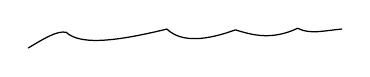
\begin{tikzpicture}[x=1cm,y=1cm,line cap=round,line join=round]
\draw[line width=0.45pt] (0,0) .. controls (0.20,0.12) and (0.36,0.22) .. (0.48,0.20)
.. controls (0.67,0.02) and (1.18,0.10) .. (1.76,0.24)
.. controls (1.95,0.06) and (2.27,0.10) .. (2.63,0.23)
.. controls (2.83,0.17) and (3.08,0.09) .. (3.42,0.25)
.. controls (3.58,0.17) and (3.75,0.22) .. (3.98,0.24);
\end{tikzpicture}}

Catégorie bordélique précisée (correspondant à un $\Pi_U$ \uline{connexe}) :

Ces objets sont les \deleted{couples $(I$, \unsure{systèmes}}\inserted{homs de gr.} profinis \deleted{(\unsure{indexés} par un ens. fini $I$) de l'hom}
\[
\mathcal E\xrightarrow{p}\Gamma
\]
(donnant naissance à une suite exacte :
\[
1\longrightarrow\pi\xrightarrow{\unsure{k|\kappa}}\mathcal E\xrightarrow{p}\Gamma
\]
)
et un ens. \inserted{fini} de sous-groupes (indexé par un ens $I$ d'indices)
\[
\mathcal E_i\overset{\rho_i}{\lhook\joinrel\longrightarrow}\mathcal E,
\]
et d'isomorphismes
\[
\mathcal E_i\cap\pi\overset{k_i}{\simeq}T(\bar K)
\]
\margin{42}

\scanpage{44}
\mspage{20}

Un hom d'un système
$(\mathcal E',p',(\mathcal E'_{i'})_{i'\in I'},(k'_{i'})_{i'\in I'})$
dans un syst.
$(\mathcal E,p,(\mathcal E_i)_{i\in I},(k_i)_{i\in I})$
est donné par par un hom
\[
f:\mathcal E'\longrightarrow\mathcal E
\]
\[
\beta_{i'}\in\mathcal E\quad(i'\in I'),\qquad\alpha\in\Gamma,
\]
tels que l'on ait les conditions :

\figure{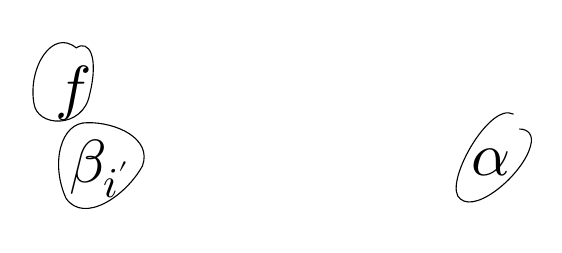
\begin{tikzpicture}[x=1cm,y=1cm,line cap=round,line join=round]
\begin{scope}[yshift=-0.35cm]
\node[font=\fontsize{22}{24}\selectfont] at (0,1.30) {$f$};
\draw (0.08,1.88) .. controls (-0.22,2.13) and (-0.53,1.64) .. (-0.46,1.19)
.. controls (-0.43,0.86) and (0.17,0.85) .. (0.25,1.29)
.. controls (0.37,1.77) and (0.24,1.99) .. (0.08,1.88);
\end{scope}
\node[font=\fontsize{22}{24}\selectfont] at (0.40,0) {$\beta_{i'}$};
\draw (0.22,0.58) .. controls (-0.12,0.59) and (-0.25,0.06) .. (-0.05,-0.38)
.. controls (0.18,-0.71) and (0.71,-0.35) .. (0.92,0.03)
.. controls (1.05,0.38) and (0.58,0.59) .. (0.22,0.58);
\node[font=\fontsize{22}{24}\selectfont] at (5.35,0.08) {$\alpha$};
\draw (5.63,0.69) .. controls (5.32,0.85) and (4.72,-0.23) .. (4.96,-0.39)
.. controls (5.18,-0.57) and (5.77,-0.05) .. (5.85,0.29)
.. controls (5.89,0.42) and (5.82,0.50) .. (5.71,0.50);
\end{tikzpicture}}

\margin{Les $\beta_{i'}$ pas uniques (si $\beta_{i'}$ convient, aussi $\gamma\beta_{i'}$, avec $\unsure{\gamma|\gamma_i}\in\operatorname{Im}k_i$). Mais $\alpha$ unique \unsure{?!|??}}

$1^\circ)$\quad $p\circ f_{\mathcal E}=\operatorname{int}(\alpha)\,p'$

$2^\circ)$\quad $\forall i'\in I',\quad\exists i\in I$ (unique!) tel que
\[
\operatorname{int}(\beta_{i'}^{-1})f(\mathcal E'_{i'})\subset\mathcal E_i
\]
et un entier $d_{i'}\in\mathbb N^*$ tel que
\[
\operatorname{int}(\beta_{i'}^{-1})f\,k'_{i'}
 =k_i\circ(d_{i'}\cdot\operatorname{id}_{T(\bar K)})
\]

\margin{NB : $d_{i'}$ est aussi unique\ldots}

\margin{[donc $\operatorname{int}(\beta_{i'}^{-1})\overbrace{\unsure{\operatorname{Im}(fk'_{i'})|\operatorname{Im}k'_{i'}}}^{L'_{i'}}\subset\underbrace{\operatorname{Im}k_i}_{L_i}$ et \unsure{même} \deleted{\unsure{cette} image} $\operatorname{int}(\beta_{i'}^{-1})\unsure{L'_{i'}}=d_{i'}L_i$.]}

\figure{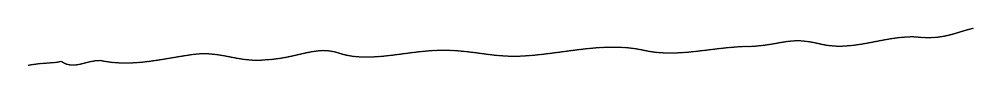
\begin{tikzpicture}[x=1cm,y=1cm,line cap=round,line join=round]
\draw[line width=0.45pt] (0,0) .. controls (0.22,0.04) and (0.30,0.02) .. (0.42,0.05)
.. controls (0.58,-0.07) and (0.73,0.07) .. (0.92,0.06)
.. controls (1.30,-0.02) and (1.64,0.07) .. (2.04,0.13)
.. controls (2.44,0.20) and (2.64,0.03) .. (3.02,0.07)
.. controls (3.43,0.09) and (3.66,0.26) .. (3.96,0.15)
.. controls (4.37,0.02) and (4.86,0.21) .. (5.35,0.19)
.. controls (5.79,0.17) and (5.95,0.08) .. (6.44,0.13)
.. controls (6.94,0.18) and (7.37,0.29) .. (7.82,0.19)
.. controls (8.26,0.09) and (8.70,0.24) .. (9.18,0.24)
.. controls (9.58,0.26) and (9.66,0.37) .. (10.06,0.27)
.. controls (10.48,0.17) and (10.87,0.38) .. (11.28,0.36)
.. controls (11.62,0.32) and (11.78,0.42) .. (12.00,0.47);
\end{tikzpicture}}

Je m'aperçois qu'il vaut mieux remplacer les $\beta_{i'}$ par les $\beta_{i'}^{-1}$, i.e. prendre l'iso. de commutation plutôt dans le sens
\[
f_{\mathcal E}\rho'_{i'}\xrightarrow{\beta_{i'}}\rho_i f_{i'}
\]
qu'en sens inverse. De plus, conceptuellement le diagramme
\diagram{\begin{tikzcd}[ampersand replacement=\&]
\& \Pi_{D^*}\arrow[dl,"\rho"']\arrow[dr,"\sigma"] \& \\
\Pi_U\arrow[dr,"\varphi"',""{name=L,inner sep=0pt}] \& \& \Pi_D\arrow[dl,"\psi",""{name=R,inner sep=0pt}]\\
\&\Pi_e\&
\arrow[from=L,to=R,bend left=25,"\alpha"]
\end{tikzcd}}
est trop compliqué, il suffit de se donner
\[
\boxed{\Pi_{D^*}\xrightarrow{\rho}\Pi_U\xrightarrow{\varphi}\Pi_e}
\]
et de déduire $\Pi_D$ par factorisation canonique
\margin{43}

\scanpage{45}

de l'hom. de groupoïdes $\Pi_{D^*}\longrightarrow\Pi_e$ en un hom qui induit un iso sur $\pi_0$ et un épi sur les $\pi_1$, suivi d'un hom qui est (épi sur $\pi_0$, et pour cause!, et qui est) \uline{fidèle}. Alors les $1$-morphismes de
\[
\Pi'_{D^*}\xrightarrow{\rho'}\Pi'_U\xrightarrow{\varphi'}\Pi_e
\]
\deleted{dans}
dans
\[
\Pi_{D^*}\xrightarrow{\rho}\Pi_U\xrightarrow{\varphi}\Pi_e
\]
sont les \deleted{\unsure{couples}}\inserted{quintuplets} de $2$ foncteurs \inserted{et $3$ iso de foncteurs}
$(f_{D^*},f_U,\alpha_{D^*U},\alpha_{Ue},K$
donnant un diagramme avec données de commutation
\diagram{\begin{tikzcd}[ampersand replacement=\&,column sep=1.05em,row sep=0.75em]
\Pi'_{D^*}\arrow[rrr,"\rho'"]\arrow[ddd,"f_{D^*}"'] \& \& \& \Pi'_U\arrow[rrr,"\varphi'"]\arrow[ddd,"f_U"'] \& \& \& \Pi_e\arrow[ddd,equal] \\
\& \& {} \& \& \& {} \& \\
\& {}\arrow[ur,bend left=25,"\alpha_{D^*U}"] \& \& \& {}\arrow[ur,bend left=25,"\alpha_{Ue}"] \& \& \\
\Pi_{D^*}\arrow[rrr,"\rho"'] \& \& \& \Pi_U\arrow[rrr,"\varphi"'] \& \& \& \Pi_e
\end{tikzcd}},

\margin{de plus, \deleted{\illegible{1}} $\pi_1(\varphi\rho)=\pi_1(\Pi_{D^*}/\Pi_e)$ peut se définir comme un syst. local \inserted{de groupes (\unsure{commutatifs|abéliens})} sur $\Pi_{D^*}$, et on peut alors \unsure{définir|écrire}
$\boxed{\unsure{\bar k|k}:(\varphi\rho)^*\unsure{T_K|\mathcal T_K}\simeq\pi_1(\varphi\rho)}$.}

\margin{avec \uline{une} condition sur le morphisme
$\pi_1(\varphi'\rho')\unsure{\simeq|\longrightarrow}\unsure{f_{D^*}^{\,*}}(\pi_1(\varphi\rho))$
induit, qui modulo les iso. de Kummer doit être la multiplication par un $d$ \unsure{indice de ramification} (qui est une application $\pi_0(\Pi'_{D^*})\longrightarrow\mathbb N^*$). [NB la multiplication par un \uline{\unsure{entier}} \unsure{positif} \illegible{5} constants\ldots]}

si on a deux tels $1$-morphismes
\[
f=(f_{D^*},f_U,\alpha_{D^*U},\alpha_{Ue})
\quad\text{et}\quad
g=(g_{D^*},g_U,\beta_{D^*U},\beta_{Ue})
\]
un \unsure{$0$-morphisme|homomorphisme} de $f$ dans $g$ est formé d'un couple de $\mu_{D^*},\mu_U$ d'isomorphismes de foncteurs
\[
\mu_{D^*}:f_{D^*}\simeq g_{D^*},\qquad
\mu_U:f_U\longrightarrow g_U
\]
compatibles avec $\alpha_{D^*U},\inserted{\beta_{D^*U},}$ et avec $\alpha_{Ue},\inserted{\beta_{Ue},}$ \deleted{et avec}
\margin{44}

\scanpage{46}
\mspage{21}

\deleted{$k,k'$ modulo multiplication par un indice de ramification} (deux conditions de compatibilité sur les deux carrés).

Si on \deleted{suppose} se borne à des $\Pi_U,\Pi'_U$ connexes, on trouve en choisissant comme plus haut un objet \inserted{$\widetilde U$} de $\Pi_U$ et un isom
\[
\boxed{\varphi(\widetilde U)\overset{\lambda}{\simeq}\Omega}
\]
(où $\Omega=\operatorname{Spec}(\bar K)$ est l'objet-repère de $\Pi_e\ldots$), un groupe $\mathcal E$ et un hom
\[
\mathcal E\xrightarrow{\varphi}\Gamma
\]
(qui est changé par autom. int. si on change $\lambda$, et $\mathcal E$ lui-= remplacé par groupe isomorphe, \unsure{d'isom.} défini \unsure{mod.} iso. int., si on change l'objet de référence $\widetilde U$). De =, choisissant un $\widetilde U_i$ dans chaque composante $i\in\pi_0(\Pi_{D^*})$, et des isom
\[
\lambda_i:\rho(\widetilde U_i)\simeq\widetilde U,
\]
on trouve des groupes $\mathcal E_i$ et des homs
\[
\mathcal E_i\xrightarrow{\rho_i}\mathcal E.
\]
Si on change $\lambda_i$, $\rho_i$ est changé par autom intérieur de $\mathcal E$. Si on change $\widetilde U_i$, $\mathcal E_i$ est remplacé par groupe isom, \inserted{l'isom} défini à aut. int. près.
\margin{45}

\scanpage{47}

Considérons les composés
\diagram{\begin{tikzcd}[ampersand replacement=\&]
\mathcal E_i\arrow[r]\arrow[rr,bend left=30,"p_i"]\&\mathcal E\arrow[r,"p"']\&\Gamma
\end{tikzcd}}
d'où noyau, \deleted{\illegible{1}} $\unsure{K|k}$ est défini par un syst. d'iso
\[
T(\bar K)\overset{k_i}{\simeq}\operatorname{Ker}p_i\qquad(i\in I)
\]
s'insérant dans une famille de suites exactes
\[
1\longrightarrow T(\bar K)\xrightarrow{k_i}\mathcal E_i\xrightarrow{p_i}\Gamma
\]
(NB l'image de $p_i$ est un ss-groupe ouvert)
$k_i$ étant compatible aux actions de $\mathcal E_i$, quand on fait opérer $\mathcal E_i$ sur $T(\bar K)$ par l'action de $\Gamma$ sur $T(\bar K)$, et sur lui-= par autom intérieurs. Introduisant également $\pi=\operatorname{Ker}p$, on trouve donc des homs de suites exactes
\diagram{$(D)$\quad\begin{tikzcd}[ampersand replacement=\&]
1\arrow[r]\&T(\bar K)\arrow[r,"k_i"]\arrow[d,"\varepsilon_i\,\deleted{\illegible{1}}"']\&\mathcal E_i\arrow[r,"p_i"]\arrow[d,"\rho_i"]\&\Gamma\arrow[d,equal]\\
1\arrow[r]\&\pi\arrow[r,"\unsure{k|\kappa}"']\&\mathcal E\arrow[r,"p"']\&\Gamma
\end{tikzcd}\qquad$i\in I$}

\deleted{Considérons}
On peut dire que $\Pi_U$ définit un ``groupe extérieur'' $[\mathcal E]$, et $\Pi_U\longrightarrow\Pi_e$ un hom de groupes extérieurs
\[
[\mathcal E]\longrightarrow[\Gamma],
\]
de = $\Pi_{D^*}$ définit un syst. de ``groupes extérieurs'' $[\mathcal E_i]$, et \deleted{\unsure{du hom}} $\Pi_{D^*}\longrightarrow\Pi_U$
\margin{46}

\scanpage{48}
\mspage{22}

un syst. d'homs extérieurs
\[
[\mathcal E_i]\longrightarrow[\mathcal E],
\]
\deleted{enfin} mais comment en termes de groupes extérieurs exprimer les données de Kummer $k_i$ ?

Revenant au \inserted{système de} diagramme $D$ (relatif à un ens d'indices $I$.) et à un $D'$ analogue (avec ens d'indices $I'$)
\diagram{$D'$\quad\begin{tikzcd}[ampersand replacement=\&]
1\arrow[r]\&T(\bar K)\arrow[r,"k'_{i'}"]\arrow[d,"\varepsilon'_{i'}"']\&\mathcal E'_{i'}\arrow[r,"p'_{i'}"]\arrow[d,"\rho'_{i'}"]\&\Gamma\arrow[d,equal]\\
1\arrow[r]\&\unsure{\pi|\pi'}\arrow[r,"\unsure{k'|\kappa'}"']\&\mathcal E'\arrow[r,"p'"']\&\Gamma
\end{tikzcd}\qquad$i'\in\unsure{I|I'}$}
un $1$-morphisme \inserted{$f$} de $D'$ dans $D$ s'explicite par

$a)$ Un hom
\[
\boxed{\boxed{f_{\mathcal E}:\mathcal E'\longrightarrow\mathcal E}}
\]
\margin{décrit le \deleted{\unsure{correspondant}} foncteur $f_U$}
[\deleted{\unsure{dép.}}\inserted{s'explicite} en termes du choix d'un isom
\[
\nu:f(\widetilde U')\simeq\widetilde U
\]
[un autre choix modifie $f_{\mathcal E}$ par un $\operatorname{int}(\beta)$, $\beta\in\mathcal E$)]

$b)$ Une \deleted{hom} application $\tau:I'\longrightarrow I$, et pour tout $i'\in I'$, posant $i=\tau(i')$, un \deleted{application}\inserted{hom de groupes}
\[
\boxed{\mathcal E'_{i'}\xrightarrow{f_{i'}}\mathcal E_i}
\]
\margin{décrit le foncteur $f_{D^*}$}
\margin{47}

\scanpage{49}

[s'explicite en termes du choix d'un iso
\[
f_{D^*}(\widetilde U'_{i'})\overset{\nu_{i'}}{\simeq}\widetilde U_i,
\]
et modifié par des $\operatorname{int}(\beta_{i'})$, $\beta_{i'}\in\mathcal E_i$, si on change $\nu_{i'}$]

$c)$ Une donnée de commutation pour
\diagram{\begin{tikzcd}[ampersand replacement=\&,column sep=0.9em,row sep=0.7em]
\mathcal E'\arrow[rrr,"p'"]\arrow[ddd,"f_{\mathcal E}"'] \& \& \& \unsure{\Gamma|\Gamma'}\arrow[ddd,equal] \\
\& \& {} \& \\
\& {}\arrow[ur,bend left=25,"{\deleted{\unsure{\beta}}\alpha}"] \& \& \\
\mathcal E\arrow[rrr,"p"'] \& \& \& \Gamma
\end{tikzcd}\quad$\boxed{\boxed{\deleted{\unsure{\beta}}\alpha\in\Gamma}}$}
\margin{$\alpha$ décrit $\alpha_{Ue}$}
i.e.
\[
\deleted{f_{\mathcal E}p'=\operatorname{int}(\unsure{\beta})p}
\qquad\boxed{pf_{\mathcal E}=\operatorname{int}(\alpha)p'}
\]

$d)$ $\forall i'[\in\unsure{I|I'}]$ une donnée de commutation pour
\diagram{\begin{tikzcd}[ampersand replacement=\&,column sep=0.9em,row sep=0.7em]
\mathcal E'_{i'}\arrow[rrr,"\rho'_{i'}"]\arrow[ddd,"f_{i'}"'] \& \& \& \mathcal E'\arrow[ddd,"f_{\mathcal E}"] \\
\& \& {} \& \\
\& {}\arrow[ur,bend left=25,"\alpha_{i'}"] \& \& \\
\mathcal E_i\arrow[rrr,"\rho_i"'] \& \& \& \mathcal E
\end{tikzcd}\quad$\boxed{\alpha_{i'}\in\mathcal E}\quad(i'\in I')$}
\margin{$(\alpha_{i'})$ décrit $\alpha_{D^*U}$}
i.e. :
\[
\boxed{\rho_i f_{i'}=\operatorname{int}(\alpha_{i'})f_{\mathcal E}\rho'_{i'}}
\]

Notons que $c,d$ ensemble définissent une donnée de commutation
\diagram{\begin{tikzcd}[ampersand replacement=\&,column sep=0.9em,row sep=0.7em]
\mathcal E'_{i'}\arrow[rrr,"p'_{i'}"]\arrow[ddd,"f_{i'}"'] \& \& \& \Gamma\arrow[ddd,equal,"{\deleted{\operatorname{int}(\unsure{\gamma})}}"] \\
\& \& {} \& \\
\& {}\arrow[ur,bend left=25,"{\operatorname{int}(\beta_{i'})}"] \& \& \\
\mathcal E_i\arrow[rrr,"p_i"'] \& \& \& \Gamma
\end{tikzcd}}
avec $\beta_{i'}=p(\alpha_{i'})\alpha$
i.e.
\[
p_i f_{i'}=\operatorname{int}(\beta_{i'})p'_{i'}
\]
\margin{48}

\scanpage{50}
\mspage{23}

i.e. on a commutativité dans
\diagram{\begin{tikzcd}[ampersand replacement=\&]
\mathcal E'_{i'}\arrow[r,"p'_{i'}"]\arrow[d,"f_{i'}"']\&\Gamma\arrow[d,"\operatorname{int}(\beta_{i'})"]\\
\mathcal E_i\arrow[r,"p_i"']\&\Gamma
\end{tikzcd}}
donc $f_{i'}$ induit un hom de suites exactes
\diagram{\begin{tikzcd}[ampersand replacement=\&]
1\arrow[r]\&T(\bar K)\arrow[r,"k'_{i'}"]\arrow[d,"f^0_{i'}"']\&\mathcal E'_{i'}\arrow[r,"\unsure{p'_{i'}|f'_{i'}}"]\arrow[d,"f_{i'}"]\&\Gamma\arrow[d,"\operatorname{int}(\beta_{i'})"]\\
1\arrow[r]\&T(\bar K)\arrow[r,"k_i"']\&\mathcal E_i\arrow[r,"p_i"']\&\Gamma
\end{tikzcd}}
\margin{795}
et il faut exprimer la compatibilité de $f^0_{i'}$ avec l'indice de ramification $d_{i'}\in\mathbb N$, on trouve
\[
\boxed{f^0_{i'}=d_{i'}\chi(\beta_{i'})\operatorname{id}_{T(\bar K)}}
\]
où
\[
\chi:\Gamma\longrightarrow\widehat{\mathbb Z}^{\,*}
\]
est le caractère canonique.

Ceci posé, déterminons, pour un $1$-morphisme
\[
f=(f_{\mathcal E},\inserted{\tau,}(f_{i'}),\alpha,(\unsure{\alpha_{i'}|\alpha_i}))
\]
et un autre
\[
f'=(f'_{\mathcal E},\tau',(f'_{i'}),\alpha',(\unsure{\alpha'_{i'}|\alpha'_i})),
\]
les $0$-morphismes de l'un dans l'autre.
\margin{49}
\scanpage{51}

\unsure{correspondant|correspondent} à des syst. d'iso.
\[
\mu_{\mathcal D^*}:f_{\mathcal D^*}\longrightarrow f'_{\mathcal D^*},\qquad
\unsure{\mu_{U^*}}\;f_U\longrightarrow g_U.
\]
Cela correspond \uline{conditions} $\tau'=\tau$, $d'_{i'}=d_{i'}$ $\forall i'\in I'$ et \unsure{à} la donnée de
\inserted{ceci résulte des autres conditions\unsure{\ldots}}
\margin{\unsure{exprimons} l'\uline{existence} d'un iso. $\mu_{\mathcal D^*}$}

\margin{décrit $\mu_U$}
a) $\boxed{\boxed{\mu\in\mathcal E}}$, définissant un iso entre
\[
f_{\mathcal E}:\mathcal E'\longrightarrow\mathcal E
\quad\text{et}\quad
f'_{\mathcal E}:\mathcal E'\longrightarrow\mathcal E
\]
i.e. \deleted{\unsure{faisant}} tel que
\[
\boxed{f'_{\mathcal E}=\operatorname{int}(\mu)f_{\mathcal E}}\,)
\]

b) $\boxed{\boxed{\mu_{i'}\in\mathcal E_i}}$ $(i'\in I',\ i=\tau(i'))$
\margin{décrit $\mu_{\mathcal D^*}$}
satisfaisant
\[
\boxed{f'_{i'}=\operatorname{int}(\mu_{i'})f_{i'}}\,),
\]
\margin{ceci implique déjà $d_{i'}=d'_{i'}$}
les $\underset{\substack{\in\\\mathcal E}}{\mu},\ \underset{\substack{\in\\\mathcal E_i}}{\mu_{i'}}$ étant liés aux $\underset{\substack{\unsure{\in|\notin}\\\mathcal E}}{\alpha},\alpha'$ \unsure{\deleted{ds}|ds} $(\in\mathcal E)$
aux $\alpha_{i'},\alpha'_{i'}$ $(\in\Gamma)$ de la façon suivante
\[
\boxed{\alpha'=p(\mu)\alpha}
\]
\[
\boxed{\alpha'_{i'}=\rho_i(\mu_{i'})\alpha_{i'}}\qquad\forall i'\in I'
\]
ou encore
\[
\boxed{\begin{cases}
p(\mu)=\alpha'\alpha^{-1}\\
\rho_i(\mu_{i'})=\alpha'_{i'}\alpha_{i'}^{-1}
\end{cases}}
\]
\margin{50}
\scanpage{52}
\mspage{24}

Notons que, comme $\rho_i$ est injectif, les deuxièmes relations, donnant les $\rho_i(\mu_{i'})$, déterminent les $\mu_{i'}$ de \uline{façon unique}, l'existence de ces $\mu_{i'}$ équivaut aux relations
\[
\boxed{\alpha'_{i'}\alpha_{i'}^{-1}\in\rho_i(\mathcal E_i)}\qquad i'\in I'.
\]

Quant à la relation $p(\mu)=\alpha'\alpha^{-1}$, elle détermine $\mu$ modulo multiplication \inserted{(à droite disons)} par un \deleted{\illegible{1}} $\mu_0\in\operatorname{Ker}p=\pi$, mais qui doit être tel que l'on ait encore
\[
f'_{\mathcal E}=\operatorname{int}(\deleted{\mu_0}\mu\mu_0)f_{\mathcal E}
\]
(en plus de $f'_{\mathcal E}=\operatorname{int}(\mu)f_{\mathcal E}$) ce qui signifie \deleted{exige} que
\[
\operatorname{int}(\mu_0)f_{\mathcal E}=\unsure{f_{\mathcal E}|f'_{\mathcal E}}
\]
i.e.
\[
\boxed{\mu_0\in\operatorname{Centr}_{\unsure{\pi}}\deleted{\operatorname{Im}}f_{\mathcal E}(\mathcal E')}
\]

C'est donc cela l'indétermination exacte dans le choix d'un $0$-morphisme \unsure{les|des} $1$-morph. \deleted{entre} $f$ et $f'$ de $\mathcal D'$ dans $\mathcal D$.
Si p.ex. on est dans les conditions où
$\pi'\longrightarrow\pi$ induit par $f_{\mathcal E}:\mathcal E'\longrightarrow\mathcal E$ \deleted{est} a une image d'indice fini (image ouverte)
--- cas d'un ``morphisme non constant'' ! ---
alors $\mu_0$ doit centraliser un ss-groupe ouvert de
\margin{51}
\scanpage{53}

$\pi$ --- sauf erreur cela aussi implique $\mu_0=1$, donc il semble bien que \deleted{\illegible{1}} (dans les cas correspondants à des hom dominants de courbes algébriques) une \deleted{hom} $0$-morphisme d'un $f$ \unsure{ds} un $f'$ (s'il existe) est unique, i.e. \uline{$\operatorname{Hom}$} $(\mathcal D',\mathcal D^*)$ est une catégorie \uline{discrète}.

On peut interpréter $\mathcal D$ comme $\mathcal E$ muni de sous-groupes $\mathcal E_i\subset\mathcal E$, et de $p:\mathcal E\longrightarrow\unsure{\Gamma_*|\Gamma}$ (noyau $\pi$) enfin d'isomorphismes
\[
k_i:\mathrm T(\overline K)\xrightarrow{\sim}\mathcal E_i\cap\pi=L_i
\]
(commutant à l'action de $\mathcal E_i$).
Si on a \unsure{une|un} autre syst.
\[
(\mathcal E',\ (\mathcal E'_{i'})_{i'\in I'},\ p':\mathcal E'\longrightarrow\Gamma',\ (k'_{i'})_{i'\in I'}),
\]
\inserted{$\mathcal E'_{i'}\subset\mathcal E'$}
un morphisme du premier dans le second est \uline{défini} par un
\[
f:\mathcal E'\longrightarrow\mathcal E
\]
satisfaisant les conditions suivantes

\inserted{b) $pf$ est conjugué de $f'$ [soit $\alpha\in\Gamma$ tel que $pf=\operatorname{int}(\alpha)p'$]}

a) $\forall i'\in I',\quad\exists i\in I$ tel que $f(\mathcal E'_{i'})$ soit contenu dans un conjugué de $\mathcal E_i$
[soit $\alpha_{i'}\in\mathcal E$ tel que
$f(\mathcal E'_{i'})\unsure{\subset|=}\operatorname{int}(\alpha_{i'}^{-1})(\mathcal E_i)$]
\inserted{i.e. $\operatorname{int}(\alpha_{i'})f(\mathcal E'_{i'})\subset\mathcal E_i$}
\margin{52}
\scanpage{54}
\mspage{25}

\uline{NB} Le $i\in I$ correspondant à $i'\in I'$ est unique, d'où $\tau:I'\longrightarrow I$.
Si les $\alpha_{i'}$ sont choisis, on déduit \deleted{\unsure{$\forall i'$}} hom induits
$f_{i'}:\mathcal E'_{i'}\longrightarrow\mathcal E_i$,
\[
f_{i'}=(\operatorname{int}(\alpha_{i'})\circ f)|\mathcal E'_{i'},
\]
qui induit dès lors, via les $k'_{i'},k_i$, un endomorphisme
\[
f^0_{i'}:\mathrm T(\overline K)\longrightarrow\mathrm T(\overline K).
\]
\margin{\uline{NB} A priori $f^0_{i'}$ est la \unsure{multiplication par} $\chi_{i'}\in\unsure{\widehat{\mathbb Z}^{\,*}|\widehat{\mathbb Z}}$. Le centralisateur dans $\Gamma$ d'un ss-groupe ouvert est réduit à l'unité.}
On exige que $\alpha\in\Gamma$ (qui conjugue $\unsure{f_{\mathcal E}}$ en $\unsure{f'_{\mathcal E}}$\}, et est \unsure{probablement} uniquement déterminé par cette condition) et $\alpha_{i'}$ (qui est sans doute déterminé mod \deleted{\unsure{conjugaison}} composition à g. avec un élt \unsure{des normalisateurs|du normalisateur} de $\mathcal E_i$ (du moins des transporteurs \inserted{des $\mathcal E_i$} d'un ss-groupe ouvert de $\mathcal E_i$ --- c'est itou si $f$ est iso) puissent être choisis de telle façon que, posant
\[
\beta_{i'}=p(\alpha_{i'})\alpha,
\]
on ait
\[
f^0_{i'}=(d_{i'}\chi(\beta_{i'}))\operatorname{id}_{\mathrm T(\overline K)}
\]
\inserted{i.e. $\chi_{i'}=d_{i'}\chi(\beta_{i'})$}
\margin{Cette condition sur les syst. des $\alpha_{i'}$ ne change pas ($\alpha$ restant fixé) si on change $\alpha_{i'}$ en $\mu_{i'}\alpha_{i'}$, où $\mu_{i'}\in\mathcal E_i$.}
$d_{i'}\in\mathbb N^*$ est un entier naturel évidemment uniquement déterminé \unsure{\}} quand $\alpha$ et les $\alpha_{i'}$ sont choisis).

\deleted{Remplaçons $\alpha$ par $\alpha'=\alpha_0\alpha$.}
\margin{53}
\scanpage{55}

8, \uline{Réflexion taxonomique.}

Le cas $\dim X=0$ se traduit sur le paradigme du système
$(\mathrm T(\overline K)\xrightarrow{k_i}\mathcal E_i\overset{\rho_i}{\hookrightarrow}\mathcal E\xrightarrow{p}\Gamma)$
\deleted{\illegible{2}} par la condition \deleted{$\unsure{\pi|I}=\varnothing$} $p$ injectif, \deleted{donc \unsure{se|de}}
\inserted{et donc $I=\varnothing$ --- donc ce cas se}
décrit \deleted{\illegible{1}}
simplement par la donnée d'un \uline{sous-groupe} ouvert $\mathcal E\subset\Gamma$, i.e. d'une sous-extension finie $\unsure{L}$ de $\overline K/K$
(NB on aura bien sûr $X'=\operatorname{Spec}\unsure{L'|L}$, et les choix \inserted{faits} sur $X$ \inserted{--- i.e. sur $\underset{=\varnothing}{\Pi_{\mathcal D^*}}\longrightarrow\Pi_U\longrightarrow\Pi_e$ ---} \unsure{aboutissant|aboutissent} à cette description --- reviennent ici au choix d'une telle \inserted{$K$-}immersion de $L\deleted{\unsure{K'}}=\mathrm H^0(X,\mathcal O_X)$ dans $\overline K/K$)

Le cas $\dim X=1$ se traduit par le fait que $\mathcal E\longrightarrow\Gamma$ n'est pas injectif --- quant à $I$, il peut être vide ou non dans ce cas.
S'il est vide, la description se fait donc simplement en termes d'un hom de groupes profinis $\mathcal E\xrightarrow{p}\Gamma$ (où $\Gamma$ donné d'avance $=\operatorname{Gal}(\overline K/K)$ \unsure{\}} $=\operatorname{Aut}_{\Pi_e}(\Omega)$).

Supposons donnés maintenant à la fois
\[
\mathcal D=(\mathcal E,p,I,(\rho_i:\mathcal E_i\hookrightarrow\mathcal E),(k_i:\mathrm T(\overline K)\longrightarrow\mathcal E_i))
\]
et
\[
\mathcal D'\unsure{=} (\mathcal E',\unsure{p'},I',(\rho'_{i'}:\ ),(k'_{i'}:\ )),
\]
et revenons à la question de la description des morphismes de $\mathcal D'$ dans $\mathcal D$.
On va distinguer quatre cas, suivant les deux valeurs
\margin{54}
\scanpage{56}
\mspage{26}

possibles $0,1$ de $n=\dim\mathcal D$ et $n'=\dim\mathcal D'$ respectivement.

I) $n=0,n'=0$, \deleted{\unsure{alors|donc}} $I=I'=\varnothing$ et les données se réduisent à des sous-groupes ouverts
$\mathcal E\overset{p}{\hookrightarrow}\Gamma$, $\mathcal E'\overset{p'}{\hookrightarrow}\Gamma$.
Dans la pesante description plus haut, \deleted{toutes} les considérations relatives à $I,I'$ tombent et \uline{les}\margin{(un)} morphisme $\mathcal D'\longrightarrow\mathcal D$ revient à une classe de \deleted{\unsure{homomorphismes}} couples $(f,\alpha)$, où
$f:\mathcal E'\longrightarrow\mathcal E$ et $\alpha\in\Gamma$, tel que l'on ait
\[
pf=\operatorname{int}(\alpha)f
\]
--- ce qui implique que $f$ est déjà déterminé par $\alpha$, étant induit par $\operatorname{int}(\alpha)$
\inserted{[$\alpha$ assujetti à $\alpha\in\operatorname{Trans}_{\Gamma}(\mathcal E',\mathcal E)$ \unsure{$=$} $\operatorname{Trans}_{\Gamma}(L,L')$]}
\deleted{\diagram{\begin{tikzcd}[ampersand replacement=\&,column sep=1.5em,row sep=2em]
\unsure{\mathcal E'}\arrow[rr,"f"]\arrow[dr,"p'"'] \& \& \mathcal E\arrow[dl,"p"] \\
\& \Gamma \&
\end{tikzcd}}}
\diagram{\begin{tikzcd}[ampersand replacement=\&]
\mathcal E' \arrow[r,"f"] \arrow[d,"p'"'] \& \mathcal E \arrow[d,"p"] \\
\Gamma \arrow[r,"\operatorname{int}(\alpha)","\sim"'] \& \Gamma
\end{tikzcd}}
[qui induit \unsure{donc|bien} un hom de $\unsure{L^*|L}\subset\overline K$ dans $L'\subset\overline K$, donc un hom $\operatorname{Spec}(L')\longrightarrow\operatorname{Spec}(L)$ en sens inverse].

La condition que $\alpha,\alpha'\in\Gamma$ définissent le même morphisme $\mathcal D'\longrightarrow\mathcal D$ (ou encore $\operatorname{Spec}\unsure{L'}\longrightarrow\operatorname{Spec}L$) se décrit par l'existence d'un $\mu\in\mathcal E$ \deleted{(= stabilisateur de} tel que $\alpha'=\mu\alpha$.
Le fait qu'on donne une corr. $1$-$1$ entre
\[
\operatorname{Hom}_{K}(X',X)\simeq\unsure{\operatorname{Hom}}_{K}(\unsure{L},L')
\]
avec $\operatorname{Hom}(\mathcal D',\mathcal D)$ explicité aussi, est clair.
\margin{55}
\scanpage{57}

II) $n'=1,n=0$.
\inserted{Ici $n=0$ implique déjà $I=\varnothing$.}
\deleted{Ici} Pour que $\operatorname{Hom}(X',X)\ne\varnothing$, il faut que l'on ait $I'=\varnothing$
[par la condition $f^{-1}(S)=S'$ qui implique $S'=\varnothing$, si $f:(X',S')\longrightarrow(X,S)$]
\inserted{$f^{-1}(\varnothing)=\varnothing$}
--- \deleted{dans} dans la description des morphismes $\mathcal D'\longrightarrow\mathcal D$, cela correspond au fait qu'on ne peut avoir d'application $\tau:I'\longrightarrow I(=\varnothing)$ que si $I'=\varnothing$.
\margin{cela on ne peut}
\deleted{\illegible{1}}
Se bornant donc au cas $I'=\varnothing$ (sinon $\operatorname{Hom}(X',X)=\operatorname{Hom}(\mathcal D',\mathcal D)=\varnothing$ et on est heureux), on trouve donc que $\mathcal D$ revient à la donnée de $\mathcal E\overset{p}{\hookrightarrow}\Gamma$ ss-groupe ouvert, et $\mathcal D'$ à la donnée d'un hom de groupes profinis $p':\mathcal E'\longrightarrow\Gamma$, dont l'image sera un ss-groupe ouvert de $\Gamma$, soit $\Gamma'_0\subset\Gamma$, correspondant à une ss-extension \inserted{finie} $L'$ de $\overline K/K$.
\margin{Se bornant donc au cas}

Les choix faits relatifs à $X'$ impliquent \unsure{précisément|qu'on a} un iso fixé $L'\simeq\mathrm H^0(X',\mathcal O_{X'})$.
Ceci dit, un $K$-morphisme \inserted{de $(X',\varnothing)$ dans $(X,\varnothing)$ i.e. de} $X'\longrightarrow X$ revient \inserted{(comme $X$ affine)} à la donnée d'un $K$-morphisme $\operatorname{Spec}L'\longrightarrow X\ (\simeq\operatorname{Spec}L)$ de l'enveloppe affine, i.e. d'un \inserted{$K$-}hom $L\longrightarrow L'$.
(ce qui ne dépend que de $L,L'$, ou encore \unsure{des} \deleted{\illegible{1}} ss-groupes $\mathcal E\subset\Gamma$ et $\Gamma_0\subset\Gamma$
\margin{56}
\scanpage{58}
\mspage{27}

de $\Gamma$).
D'autre part la description en termes des diagrammes $\mathcal D,\mathcal D'$ revient à dire qu'un morphisme est déterminé par un couple $(f,\alpha)$, $f:\mathcal E'\longrightarrow\mathcal E$ et $\alpha\in\Gamma$, tels que l'on ait encore commutativité
\diagram{\begin{tikzcd}[ampersand replacement=\&]
\mathcal E' \arrow[r,"f"] \arrow[d,"p'"'] \& \mathcal E \arrow[d,hook,"p"] \\
\Gamma \arrow[r,"\operatorname{int}(\alpha)"] \& \Gamma
\end{tikzcd}}
\[
pf=\operatorname{int}(\alpha)p'
\]
ce qui implique encore que $f$ est déterminé par $\alpha$ (savoir, induit par $\operatorname{int}(\alpha)$), et $\alpha$ étant sujet à la seule condition
\[
\alpha\in\operatorname{Transp}_{\Gamma}(\Gamma'_0,\mathcal E)
\]
--- et $\alpha,\alpha'$ \unsure{décrivant|décrivent} le $=$ hom \unsure{ssi}
\[
\exists\mu\in\mathcal E\quad\text{tel que}\qquad\unsure{\Longleftarrow|\Longleftrightarrow}
\]
\[
\alpha'=\mu\alpha
\]
donc on a encore
\[
\begin{aligned}
\operatorname{Hom}(\mathcal D',\mathcal D)
&\simeq\mathcal E\backslash\operatorname{Transp}_{\Gamma}(\Gamma'_0,\Gamma)\ \deleted{\illegible{1}}\\
&\simeq\operatorname{Transp}_{\Gamma}(L,L')/\operatorname{Fix}_{\Gamma}(L)\\
&\simeq\operatorname{Hom}_{\unsure{K\text{-}\mathrm{ext}|K\text{-}\mathrm{cat}}}(L,L')
\end{aligned}
\]
donc on trouve encore dans ce cas \unsure{le|la} pleine fidélité.

En fait, on aurait pu traiter ensemble
\margin{57}
\scanpage{59}

les deux cas $(n'=0,n'=1)$ où $n=0$, et la description des $\operatorname{Hom}(X,X')$ \inserted{en termes de $\mathcal D,\mathcal D'$} est valable d'ailleurs, sans \deleted{supposer que} faire des hypothèses draconiennes (projectif, lisse, $\dim\leq1$, anabélien) sur $X'$.
\deleted{Il suffit que $X'$ soit un schéma connexe quasi-compact quasi-séparé sur $K$, \unsure{donc|dans} les morphismes $X'\longrightarrow X=\operatorname{Spec}(L)$ correspondent aux morphismes $\operatorname{Spec}A'\longrightarrow X$ de l'enveloppe affine de $X'$ dans $X$, définie comme Spectre de $A'=\mathrm H^0(X',\mathcal O_{X'})$, i.e. aux \unsure{$K$-hom} de $K$-algèbres
\[
L\longrightarrow A'.
\]}

En effet, comme $X$ est \inserted{fini} étale sur $K$, son image inverse \inserted{$X_{X'}=$} \deleted{\illegible{1}} $X'\times_K\unsure{X}$ sur $X'$ est \inserted{fini} étale sur $X'$, et
\[
\operatorname{Hom}_K(X,X')\simeq\deleted{\operatorname{Hom}\unsure{(}}\operatorname{Sections}(X_{X'}/X')
\]
peut se décrire en termes de la catégorie $\widehat{\Pi_1(X')}$ $(=\Pi_U)$ des syst. locaux finis sur $X'$ i.e. des syst. locaux finis sur $\Pi_U$.
Suivant cette description, on aboutit à la
\margin{58}
\scanpage{60}
\mspage{28}

description commune donnée dans I, II, sans aucune hyp. autre sur $X$ que \deleted{la connexité} la $0$-connexité (pour pouvoir décrire $\Pi_U=\Pi_{X'}$ sur $\Pi_e$ en termes d'un hom de groupes $p':\mathcal E'\longrightarrow\Gamma\ldots$).

Quand on se donne $(X',S')$, avec $S'$ pas nécessairement vide, $X'$ $0$-connexe (et \deleted{dim} $X'$ lisse de dim $1$ aux pts de $S'$ (il suffirait $=$ que $S'$ \unsure{ne} \unsure{disconnecte|déconnecte} pas localement \inserted{(ét)} $X'$, $\ldots$),
\inserted{donc $X'-S'$ $0$-connexe}
alors la \deleted{partie} donnée
$\Pi_1(X'-S')\longrightarrow\Pi_1(e_K)$ est décrite \deleted{\illegible{1}} par $\mathcal E'\xrightarrow{p'}\Gamma$ (indépendamment de la considération des $\mathcal E_i$ etc) et par suite $\operatorname{Hom}_K(X'-S',X)$ est décrit comme on vient de dire.
Mais on a (avec les hypothèses de normalité de $X'$ aux pts de $S'$)
\[
\operatorname{Hom}_K(X'-S',X)=\operatorname{Hom}_K(X',X).
\]

Ceci encourage à modifier la définition des morphismes $(X',S')\longrightarrow(X,S)$ donnée \unsure{au|par} début, via $f:X'\longrightarrow X$ avec $f^{-1}(S)_{\mathrm{r\acute ed}}=S'$, en exigeant ceci \inserted{non pour $f$, mais} \unsure{seulement} pour la restriction de $f$ \unsure{à} la réunion des comp. irréd. de $X'$
\margin{59}
\scanpage{61}

\deleted{sur lesquelles $f$ n'est pas ``\unsure{constante|constantes}''}
qui sont envoyées dans des comp. irréductibles de $X$ \deleted{\illegible{1}} non discrètes i.e. non réduites à un pt.
Dans la description correspondante $\mathcal D'\to\mathcal D$, on spécifiait que l'on n'exige la donnée d'une application $I'\to I$ (et des données correspondantes $f_{i'},\alpha_{i'}$) \uline{que} si \deleted{\unsure{$I\ne\varnothing$}} $n\ne0$ i.e. \unsure{$p_{si}$|$p_X$}$:\mathcal E\to\Gamma$ pas injectif, --- dans le cas contraire (impliquant $I=\varnothing$) \inserted{si par hasard $I'\ne\varnothing$,} on laisse tomber la connaissance de $I'$ et des éléments de structure correspondants.

\uline{$\overline{\mathrm{III}}$}) $n'=0$, $n=1$. Ici on a donc $I'=\varnothing$, $p':\mathcal E'\hookrightarrow\Gamma$ i.e. $\mathcal D'$ se réduit à la donnée d'un ss-gr. ouvert $\mathcal E'\hookrightarrow\Gamma$ de $\Gamma$.
Du côté $(X',S'=\varnothing)$ et $(X,S)$, la condition $f^{-1}(S)_{\mathrm{r\acute ed}}=S'=\varnothing$ sur \inserted{le $K$-morphisme} $f:X'\to X$ implique que $f$ se factorise par $X'\Longrightarrow\operatorname{Spec}(L')\longrightarrow X\setminus S$, sans préjudice si $S=\varnothing$ ou non, i.e. si $I=\varnothing$ ou non. Donc il s'agit de décrire $\operatorname{Hom}_{K\text{-sch}}(X',X\setminus S)$, en termes de $\begin{gathered}\text{\inserted{$\Pi_{U'}$}}\\[-2pt]\rotatebox{90}{$=$}\\[-2pt]\Pi_1(X')\end{gathered}\to\Pi_e=\Pi_1(e_K)$

\margin{60}

\scanpage{62}
\mspage{29}

et de $\begin{gathered}\text{\inserted{$\Pi_U$}}\\[-2pt]\rotatebox{90}{$=$}\\[-2pt]\Pi_1(X\setminus S)\end{gathered}\to\Pi_e$.
Ici les éventuelles données supplémentaires relatives à $I$ ne servent pas explicitement à la description, en termes de diagrammes \inserted{(de groupoïdes)}.
Sauf erreur, une réduction facile \inserted{(descente galoisienne)} nous ramène au cas où $X'=\operatorname{Spec}K$ i.e. $\mathcal E'\Leftrightarrow\Gamma$. La description \unsure{des|en} hom. $\mathcal D'\to\mathcal D$ est alors \inserted{encore} en termes de couples $(f,\alpha)$, où $f:\mathcal E'=\Gamma\to\mathcal E$ et où $\alpha\in\Gamma$, avec la sempiternelle condition $pf=\operatorname{int}(\alpha)p'$, qui devient (comme $p'=\operatorname{id}$)
\[
 pf=\operatorname{int}(\alpha).
\]

\deleted{\unsure{$\alpha$ et $\alpha'$}}
Ici bien sûr $\alpha$ ne décrit plus $f$ (mais l'inverse est \deleted{sans doute} vrai, ici la connaissance de $f$ donc de $pf\in\operatorname{Aut}(\Gamma)$ implique celle de $\alpha$, i.e. $\operatorname{Cent}(\Gamma)=\{1\}$ \ldots).
Les couples $(f,\alpha)$ et $(f',\alpha')$ définissent le $=$ morphisme de diagrammes, sss $\exists\mu\in\mathcal E$ tel que $f'=\operatorname{int}(\mu)\circ f$, $\alpha'=p(\mu)\alpha$.
Comme (si $\exists(f,\alpha)$) $p$ est surjectif,

\margin{61}

\scanpage{63}

on \unsure{voit|veut} que, quitte à choisir $\mu$ au dessus de \deleted{\illegible{1}} $\alpha^{-1}$, et de remplacer $(f,\alpha)$ par $(f',\alpha')=(\operatorname{int}(\mu)f,p(\mu)\alpha)$, on peut tjrs décrire un morphisme $\mathcal D'\to\mathcal D$ par $(f,\alpha)$ avec $\alpha=1$ donc par une \uline{section} $f$ de l'hom. $\mathcal E\to\Gamma$, et deux sections $f,f'$ (correspondant à $(f,1),(f',1)$) définissent le $=$ hom. de \unsure{$\mathcal D'$} dans $\mathcal D$, sss $\exists\mu\in\mathcal E$ tel que $p(\mu)=1$ i.e. $\mu\in\pi=\operatorname{Ker}(p)$, et tel que $f'=\operatorname{int}(\mu)\circ f$.

Ainsi, les morphismes de $\mathcal D'$ (correspondant à $X'=\operatorname{Spec}K$) dans $\mathcal D$ correspondent exactement aux classes de scindages de $\mathcal E\xrightarrow{p}\Gamma$, mod. autom. intérieurs par des $\mu\in\pi=\operatorname{Ker}p$. La ``conjecture bordélique'' dans le cas \uline{$\overline{\mathrm{III}}$} équivaut donc à ceci:
\margin{\figure{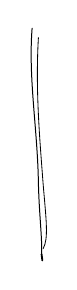
\begin{tikzpicture}[x=1cm,y=1cm,line cap=round]
\draw[line width=.36pt] (0,0) .. controls (-.05,-.64) and (.07,-1.29) .. (.08,-1.97)
 .. controls (.09,-2.38) and (.13,-2.67) .. (.12,-2.87);
\draw[line width=.30pt] (.08,-.12) .. controls (.04,-.79) and (.10,-1.44) .. (.14,-1.98)
 .. controls (.18,-2.45) and (.21,-2.67) .. (.14,-2.80);
\draw[line width=.65pt] (.12,-2.87) -- (.13,-2.95);
\end{tikzpicture}}}
\deleted{\unsure{$\operatorname{Hom}(K$}}
\[
 \Gamma((X,S)/K)\longrightarrow
 \begin{gathered}
 \text{Classes de $\pi$-conjugaison de}\\
 \text{sections de }\mathcal E\to\Gamma\text{ i.e.}\\
 \text{de sections de }\Pi_1(X)\to\Pi_1(e_K)
 \end{gathered}
\]

\margin{62}

\scanpage{64}
\mspage{30}

est bijective (si $(X,S)$ est un couple permis ``anabélien'').
\margin{faux tel quel, cf n° 9 ci-dessous --- il faut des conditions supplémentaires sur les $f$ \ldots\ \uline{Peut-être} \unsure{vrai si} $I=\varnothing$}

Je sais en tous cas que cette application est \uline{injective} --- ceci vaut chaque fois qu'on a un schéma $U$ sur $K$ (ici $X\setminus S$) qui se plonge dans un \inserted{groupe algébrique $G$} extension d'une VA par un tore, et résulte alors du th. de Mordell-Weil ``absolu'': $G(K)$ est un $\mathbb Z$-module de type fini.
En fait, il suffit de connaître la classe de splittage de l'extension $\mathcal E^{\natural}$ de $\Gamma$ par
\[
 \pi_{\mathrm{ab}}=\pi/\overline{[\pi,\pi]}\simeq H_1(\unsure{\mathrm{Alb}|U}),
\]
\deleted{\unsure{pour en déduire}} \inserted{correspondant} à un pt de $U$ rat/$K$, pour connaître ce point. Donc la \inserted{résultat de} fidélité est obtenu, avec des hyp. moins draconiennes sur $X$ que l'hyp. anabélienne (avec les notations du lemme 5.2, cela signifie que $g=0\Rightarrow\unsure{n|\nu}\ge2$ i.e. qu'il n'y a pas de comp. irréd. de \unsure{$X_{\overline K}$|$U_{\overline K}$} qui soit isom. à \unsure{$\mathbb P^1_{\overline K}$} ou $\mathbb E^1_{\overline K}$ \ldots).

\margin{63}

\scanpage{65}

\uline{NB} Ceci suggère une approche de la conjecture de Mordell, via une meilleure connaissance des extensions de $\Gamma$ par $\pi$: le fait qu'il n'y ait (pour $g\ge2$) qu'un nb fini de classes de $\pi$-conjugaison de scindages d'une telle extension \ldots.
Idem pour une approche du th. de Fermat, via \deleted{\illegible{1}} une bonne connaissance d'une extension de $\Gamma$ par $\pi=\pi_1(\unsure{\mathbb P^1_{\overline{\mathbb Q}}\setminus\{0,1,\infty\}})$ \ldots.

\uline{Cas $\overline{\mathrm{IV}}$} $n=1,n'=1$ i.e. $X,X'$ de dim 1.

a) Si $I=I'=\varnothing$, je n'ai rien à ajouter à la description des morphismes $f:X\to X'$ en termes de morphismes de diagrammes de groupoïdes. Ici \deleted{\illegible{1}} la condition $f^{-1}(S)_{\mathrm{r\acute ed}}=S'$ n'est pas une restriction sur $f$ --- \deleted{qui} on n'exclut donc pas des applications constantes. Celles-ci (grâce à
\margin{(grâce à \ldots)}
\deleted{Si \unsure{$I'\ne\varnothing$} \illegible{5} \unsure{seulement} $I'=\varnothing$ \inserted{\unsure{i.e. $S'=\varnothing$}} \illegible{7} \unsure{$S'$ est} \unsure{vide}), \unsure{donc} la condition}

\margin{64}

\scanpage{66}
\mspage{31}

l'étude \unsure{du|des} cas \uline{$\overline{\mathrm{II}}$}) sont d'ailleurs décrites de façon ``pleinement fidèle'' par des hom. de diagrammes --- Ils correspondent aux cas $f:\mathcal E'\to\mathcal E$ qui sont nuls sur $\pi'$.

b) Le cas $I'=\varnothing$, $I\ne\varnothing$ (i.e. $S'=\varnothing$, $S\ne\varnothing$) signifie, pour la condition $f^{-1}(S)_{\mathrm{r\acute ed}}=S'$ i.e. $f^{-1}(S)=\varnothing$, que $f$ doit appliquer $X'$ dans $X\setminus S$, \deleted{On s'attend donc} donc que les $f$ correspondant à un morphisme de $(X',\varnothing)$ dans $(X,S)$ sont constantes.
La conj. bordélique dans ce cas exprime donc \deleted{que} essentiellement qu'au niveau des hom. $\mathcal E'\xrightarrow{p'}\Gamma$ et $\mathcal E\xrightarrow{p}\Gamma$, tout hom. de groupes $\mathcal E'\xrightarrow{f}\mathcal E$ tel que $pf=\operatorname{int}(\alpha)p'$ pour $\alpha\in\Gamma$ [on est ramené au cas où $\alpha=1$, \inserted{$p,p'$ surjectifs} i.e. aux hom d'extensions de $\Gamma$ par \unsure{les|des} groupes \unsure{$\pi=\pi_1(\overline{X\setminus S})$} et $\pi'=\pi_1(\overline X')$)] est trivial sur $\pi'$ [i.e. ``est'' une section]. Il faudrait essayer de vérifier ce point directement, qui (modulo le cas \uline{$\overline{\mathrm{III}}$}) établirait la ``conj. bordélique'' dans ce cas-là.

\margin{65}

\scanpage{67}

c) Le cas $I'\ne\varnothing$, $I=\varnothing$ implique que $\operatorname{Hom}((X,S),(X',S'))=\varnothing$ (car $f^{-1}(S)=f^{-1}(\varnothing)=\varnothing\ne S'$ !), ce qui correspond bien \deleted{au cas} à $\operatorname{Hom}(\mathcal D',\mathcal D)=\varnothing$ puisque $\nexists\tau:I'\to I$.

d) Dans le cas $I'\ne\varnothing$, $I\ne\varnothing$, la condition $f^{-1}(S)_{\mathrm{r\acute ed}}=S'$ implique que $f$ n'est pas constante (sinon on aurait $f^{-1}(S)_{\mathrm{r\acute ed}}=\varnothing$ ou $X'$), donc $f$ est dominant et fini, génériquement étale. [Donc, de telles $f$ ne \deleted{\unsure{sont admis} \illegible{1}} peuvent intervenir que si $I$ et $I'$ sont soit tous deux $\varnothing$ (cas a)), soit tous deux $\ne\varnothing$ (cas actuel d)). Le fait que dans ces cas là, la description diagrammatique galoisienne soit \uline{fidèle} (peut-être pas pleinement) résulte aisément du résultat analogue dans le cas \uline{$\overline{\mathrm{III}}$}.
La pleine fidélité par contre est chose mystérieuse, $=$ si le résultat correspondant \deleted{\unsure{dans}} \deleted{\illegible{1}} au cas \uline{$\overline{\mathrm{III}}$} était acquis (\unsure{et on en}

\margin{66}

\scanpage{68}
\mspage{32}

semble loin, $=$ si $K$ fini sur $\mathbb Q$ \ldots)

\uline{Réductions} \uline{élémentaires} Pour prouver la ``conj. bordélique'', on est ramené (par des ext. finies des corps $K$) au cas où $\mathcal E\to\deleted{\unsure{K}}\Gamma$ (et, si on y tient, aussi $\mathcal E'\to\Gamma$) est épi. Sauf erreur, la connaissance du cas \uline{$\overline{\mathrm{III}}$} pour des extensions de t.f. de $K$, implique le cas général pour $K$ (avec suffisamment de sueurs techniques \ldots).

Revenant cependant au cas général quand $\mathcal E\to\Gamma$ est surjectif, dans tte classe d'équival. de systèmes $(f:\mathcal E'\to\mathcal E,\alpha\in\Gamma,$ \deleted{\unsure{$f_i$,}} $\tau:I'\to I,$ \deleted{\unsure{$f_{i'}:\mathcal E'_{i'}$}} $(\alpha_{i'}\in\mathcal E_{\unsure{\tau(i')=i}})_{i'\in I'})$, on peut trouver un système avec $\alpha=1$, de sorte que $f:\mathcal E'\to\mathcal E$ est compatible avec les hom. dans $\Gamma$ (i.e. les structures d'extensions).
Quand on se borne à de tels syst., \unsure{l'|leur} équivalence par conjugaison se fait par un système \unsure{$(\mu,(\mu_{i'})_{i'\in I'})$} avec \uline{$\mu\in\pi$} $(=\operatorname{Ker}p)$, et

\margin{67}

\scanpage{69}

les $\mu_{i'}\in\mathcal E_{i=\tau(i')}$ comme avant. Ainsi, $f:\mathcal E'\to\mathcal E$ est \deleted{défini par des} \inserted{un} hom. d'extensions, défini mod autom. intérieurs par un élément de $\pi=\operatorname{Ker}(\mathcal E\to\Gamma)$, et satisfaisant des conditions explicitées par ailleurs.
Il se pourrait (comme on a déjà remarqué) que la connaissance de la \deleted{\illegible{1}} classe de $\pi$-conj. de $f$ suffise à déterminer le ``morphisme bordélique'' dans lequel $f$ s'insère (si $I,I'\ne\varnothing$).

[C'est lié à la question de savoir si le \deleted{\illegible{1}} \deleted{\unsure{tran}} $\forall d\in\mathbb N^*,\ \operatorname{Trans}_{\mathcal E}(L_i^d,L_i)$ est réduit à $\mathcal E_i$ (où $L_i=\operatorname{Ker}(p_i:\mathcal E_i\to\Gamma)=\operatorname{Im}(\kappa_i:T(\overline K)\to\mathcal E_i)$).
\margin{\deleted{Il suffirait que $\operatorname{Transp}(L_i^d,L_i)\cap\operatorname{Transp}(\unsure{\mathcal E}$}}
Dans ce cas, $\mathcal E_i$ serait connu en termes de $L_i\subset\pi$, et $=$ en termes des \unsure{rayons|noyaux} de ss-groupes qu'il définit dans $\pi$, et a fortiori en termes des \unsure{rayons|noyaux} d'hom. \unsure{défini} par $\kappa_i:T(\overline K)\to\pi$ \ldots.

\margin{68}

\scanpage{70}
\mspage{33}

\uline{Cas où} \inserted{les} $\mathcal E_i\to\Gamma$ \deleted{est} \uline{surjectif} (i.e. \inserted{les} \unsure{$k(s_i)=K$} i.e. $s_i$ rat. sur $K$).
Alors, si $(f,$ \deleted{\unsure{$\alpha$,}} $\tau,$ \deleted{\illegible{1}} $(\alpha_{i'}))$ est un hom de $\mathcal D'$ dans $\mathcal D$, \deleted{\unsure{pour} \illegible{1}} quitte à \deleted{\unsure{modifier}} \inserted{corriger} par des $\mu_i\in\mathcal E_i$ ayant $=$ image que les $\alpha_{i'}$ dans $\Gamma$, \unsure{OPS} $\alpha_{i'}\in\pi$, en plus de \unsure{$\alpha=1$} (obtenu en corrigeant par $\mu$ convenable).
Donc on décrit l'hom \inserted{$\mathcal D'\to\mathcal D$} par $(f,1,\tau,(\alpha_{i'}))$, les $\alpha_{i'}\in\pi$. La \deleted{\unsure{systèmes}} \inserted{condition} \deleted{\illegible{1}} ici est que $f:\inserted{\mathcal E'\to\mathcal E}$ soit un hom. de groupes sur $\Gamma$, que \deleted{\unsure{$\operatorname{int}(\alpha_{i'}^{-1})$}} $f(\mathcal E'_{i'})\subset\text{\inserted{$\operatorname{int}(\alpha_{i'}^{-1})$}}(\mathcal E_{\tau(i')=i})$, et que l'hom induit \inserted{$\mathcal E'_{i'}\to\mathcal E_i$} par \deleted{\unsure{$f_i=$}} \unsure{$\operatorname{int}(\alpha_{i'})f$|$\operatorname{int}(\alpha_{i'}^{-1})f$} \deleted{\unsure{de $\mathcal E_i$ de}} induit sur $T(\overline K)$ (\uline{via} $\kappa_{i'},\kappa_i$) \uline{l'hom de multiplication par $d_i$} sans plus --- que c'est beau!
Deux systèmes $(f,\tau,(\alpha_{i'}))$ et $(f',\tau',(\alpha'_{i'}))$ définissent le $=$ morphisme, sss \inserted{$\tau=\tau'$ et s'il} existe
\[
 \boxed{\mu\in\pi,\quad\mu_{i'}\in\begin{gathered}L_{i=\tau(i')}\\[-2pt]\rotatebox{90}{$=$}\\[-2pt]\text{\inserted{$\kappa_i(T(\overline K))$}}\end{gathered}}
\]
tels que
\[
 f'=\operatorname{int}(\mu)f
\]
\[
 \alpha'_{i'}=\mu_{i'}\alpha_{i'}.
\]

\deleted{\illegible{1}} Notons qu'à priori, pour $(f,\tau)$ fixé, les $\alpha_{i'}$ sont déterminés mod multiplication à droite par des éléments de $\operatorname{Transp}_{\pi}(\deleted{\unsure{\pi}}(\unsure{L_i^{d_{i'}}},L_i)$,

\margin{69}
\scanpage{71}

qui est sans doute $=L_i=\operatorname{Ker}(p_i:\mathcal{E}_i\to\Gamma)=$ \unsure{1|l'} $\operatorname{Im}(\kappa_i:T(\overline{K})\to\mathcal{E}_i\cap\pi)$.
Donc on trouve que \deleted{\unsure{$f$}} la classe de \deleted{hom.} $\pi$-conjugaison de groupes sur $\Gamma$ de $f:\mathcal{E}'\to\mathcal{E}$ suffit à déterminer l'hom $\mathcal{D}'\to\mathcal{D}$ dans la cat. bordélique.
Je présume qu'un peu de sueur permettrait de prouver que cela marche encore dans le cas général (sans supposer les $\Gamma_i=\operatorname{Im}(\unsure{\mathcal{E}_i}\to\Gamma)$ égaux à $\Gamma$).
Cela signifie (dans le cas actuel) que la structure essentielle qui décrit $(X,S)$ est celle d'\deleted{\illegible{1}} ``\uline{extension extérieure}'' de $\Gamma$ par un groupe $\pi$ [hom. ext. surjectif d'un groupe, de noyau un $\pi$], avec $\pi$ muni d'une \uline{structure à lacets} i.e. \deleted{classe de conjugaison} \inserted{d'hom.} \uline{extérieurs}
\[
\kappa_i:T\,\unsure{\text{\deleted{\illegible{1}}}|\mu}\,(=T(\overline{K})\,\unsure{\text{\deleted{)}}}\,\overset{\text{non canon}^{t}}{\simeq}\,\widehat{\mathbf{Z}})\to\pi
\]
(satisfaisant certaines conditions), les

\margin{70}

\scanpage{72}
\mspage{34}

hom \inserted{de} $\mathcal{E}'\to\Gamma$ (noyau $\pi'$) dans $\mathcal{E}\to\Gamma$ (noyau $\pi$) étant les classes de $\pi$-conjugaison d'homomorphismes $\mathcal{E}'\to\mathcal{E}$ de groupes sur $\Gamma$, induisant des hom $\pi'\to\pi$ compatibles avec la structure à lacets.

9. Structure tangentielle en les $s\in S$.
\margin{[Les sections d'extensions ``de deuxième type'']}

Revenant à la description \inserted{``intrinsèque''} des $(X,S)$ par
$\Pi_{D^*}\to\Pi_U\to\Pi_e$, un $s_i\in S$ correspond donc à une comp. connexe \inserted{$\Pi_{D_i^*}$} de $\Pi_{D^*}$, ou \inserted{un $\Pi_{D_i}$} de son quotient $\Pi_D$ --- considérons
\[
\Pi_{D_i^*}\xrightarrow{\unsure{\sigma_i=\Pi_{f_{D_i^*D_i}}|\sigma_i=\sigma_{D_i^*D_i}}}\Pi_{D_i}.
\]
On va décrire certaines sections (à isom. près) de ce \deleted{\unsure{fonct}} \inserted{morphisme} de groupoïdes, i.e. des \inserted{couples $(\gamma,\lambda)$} foncteurs
$\Pi_{D_i}\xrightarrow{\gamma}\Pi_{D_i^*}$ et d'une iso. $\sigma_i\circ\gamma\overset{\lambda}{\simeq}\operatorname{id}$.
Si on choisit un $\widetilde{D}_i^*\in\operatorname{Ob}\Pi_{D_i^*}$ (rev. universel de $D_i^*$) d'où hom \inserted{surj.}
\[
\mathcal{E}_i=\operatorname{Aut}(\widetilde{D}_i^*)\to\Gamma_i
=\operatorname{Aut}(\sigma_i(\widetilde{D}_i^*)=\widetilde{D}_i),
\]
\unsure{la} \deleted{donnée} donnée de $(\gamma,\unsure{\lambda_i|\lambda})$, \inserted{et d'une iso $\gamma(\widetilde{D}_i)\simeq\widetilde{D}_i^*$ donnant l'isom identique par application des $\sigma_i$,} revient à celle d'un hom $\Gamma_i\to\mathcal{E}_i$.
--- et les classes d'isomorphismes des couples $(\gamma,\lambda)$ correspondent aux classes de \inserted{$L_i$}-conjugaison

\margin{71}

\scanpage{73}

($L_i=\operatorname{Ker}(\text{\deleted{\illegible{1}}\inserted{$\mathcal{E}$}}_i\to\Gamma_i)$) de \deleted{morphismes} \inserted{sections} de l'ext. $\mathcal{E}_i$ de $\Gamma_i$ par $L_i$.

Ceci posé, \unsure{on a}
\[
\Gamma_i=\operatorname{Gal}(\overline{K}_i/K_i).
\]
où $K_i=k(s_i)$, $\overline{K}_i$ est la clôture algébrique de $K_i$ définie par $\widetilde{D}_i$ (à priori, elle n'est pas \unsure{can\textsuperscript{t}.} isom. à $\overline{K}$ sur $K$\ldots), et les classes de \deleted{\unsure{extensions}} \inserted{scindages} d'extensions forment un \uline{torseur} \inserted{$\Sigma_i$} (s'il y en a, et on sait qu'il y en a\ldots) sous $H^1(\Gamma_i,L_i)$, ou encore, comme $\kappa_i:L_i\xleftarrow{\sim}T(\overline{K}_i)$, sous
\[
H^1(\operatorname{Gal}(\overline{K}_i/K_i),T(\overline{K}_i))
\simeq H^1(K_i,\unsure{T_e|T_\ell}(G_m))
\simeq\varprojlim_n H^1(K_i,\mu_n).
\]
Or la suite exacte de Kummer donne
\diagram{\begin{tikzcd}[ampersand replacement=\&,column sep=small]
0 \arrow[r] \& H^0(K_i,\text{\deleted{\unsure{$\overline{K}$}}}\,G_m)_n \arrow[r] \arrow[d,equal] \& H^1(K_i,\mu_n) \arrow[r] \& {}_nH^1(K_i,G_m) \arrow[r] \arrow[d,equal] \& 0 \\
\& (K_i^*)_n \&\& 0 \&
\end{tikzcd}}
i.e. $H^1(K_i,\mu_n)\simeq(K_i^*)_n$, donc
\[
H^1(K_i,T(G_m))\simeq\varprojlim_n(K_i^*)_n
\]

\margin{72}

\scanpage{74}
\mspage{35}

Notons qu'on a un hom kummérien
\[
K_i^*\to\underbrace{H^1(K_i,T(G_m))}_{\mathcal{H}_i}
\simeq\varprojlim(K_i^*{}_n)
\]
dont le noyau est formé des $\unsure{x}\in K_i^*$ tels que pour $\forall\ n\in\mathbf{N}$, on ait $x\in K_i^{*n}$.
Comme $K_i$ est de t.f. sur $\mathbf{Q}$, cet hom est injectif, i.e. $K_i^*$ s'identifie à un sous-groupe de $\mathcal{H}_i$.

Ceci posé, \unsure{on va} définir, dans le torseur $\Sigma_i$ sous $\mathcal{H}_i$ des scindages de $D_i^*$ sur $D_i$, un sous-\inserted{$K_i^*$}-torseur (i.e. un élément de $\Sigma_i/K_i^*$).
Pour ceci,

\deleted{notons que $\mathcal{O}_{s_i}=\widehat{\mathcal{O}}_{X,s_i}$ contient canoniquement le sous-corps $K_i$ (p.ex. comme clôture entière de $K$ dans $\mathcal{O}_{s_i}$), et que le choix d'une uniformisante $t$ de $\mathcal{O}_{s_i}$ définit un \deleted{sous-corps} \inserted{$K_i$-}\deleted{$K[[t$} isom $\mathcal{O}_{s_i}\simeq K_i[[T]]$, (par la condition $T\mapsto t$). Notons que l'on a}

\margin{73}

\scanpage{75}

\deleted{(avec $\widetilde{D}_i^*$) une clôture algébrique \inserted{$\overline{K}_s$} de $K_s$ (corps des fractions de $\mathcal{O}_s$), définissant \deleted{\unsure{juste} \illegible{1}} \inserted{une} clôture alg. $\unsure{\overline{K}_i}$ de $K_i=k(s)$, \unsure{qui n'est} justement que $\overline{K}_i$. \deleted{Ceci posé, dans $\overline{K}_s$ le sous-corps}}
\margin{faire un raisonnement local général, en laiss. tomber l'indice \unsure{$i$}.}

Considérons plus généralement le cas d'un corps $k$ $(=K_i)$ de car. $0$, et d'une \deleted{\illegible{1}} $k$-algèbre $\mathcal{O}$ qui est \inserted{jauge} hensélienne de corps résiduel $k$.
\inserted{soit $L$ le corps des fractions de $\mathcal{O}$}
On va, pour \unsure{t\textsuperscript{te}} uniformisante $t$ de $\mathcal{O}$, définir une section $(\gamma,\lambda)$ \unsure{du|des} \deleted{\unsure{$\Pi_K$}} \deleted{\unsure{la caté}} \unsure{groupoïde|groupoïdes} des clôtures alg. de $L$, vers celui des rev. universels de $\unsure{\operatorname{Spec}(\mathcal{O})|\operatorname{f\acute{e}t}(\mathcal{O})}$ ou, ce qui revient au même, des clôtures alg. de $k$. Pour ceci,

soit
\[
\mathcal{O}(n,\unsure{t|s})=\mathcal{O}[T_n]/(T_n^n-s),\quad\text{et}
\]
\[
\mathcal{O}(\infty,t)=\varinjlim_n\mathcal{O}(n,t),\quad
\text{par }T_{n\,\unsure{t|s}}\mapsto T_{mn\,\unsure{t|s}}^{\,m}.
\]
\deleted{alors $\mathcal{O}(\infty,t)$ est \unsure{encore une} jauge hensélienne}
\deleted{\unsure{Posons}}
$L(n,t)=\mathcal{O}(n,t)\otimes_{\mathcal{O}}K=$ corps des fractions de $\mathcal{O}(n,t)$, $L(\infty,t)=\varinjlim_n L(n,t)$ le corps des fractions de $\mathcal{O}(\infty,t)$. C'est

\margin{74}

\scanpage{76}
\mspage{36}

une ext. alg. de $L$, et pour \unsure{t\textsuperscript{te}} \deleted{clôture alg. $\overline{k}$ de $k$, \illegible{1} $L\otimes_k\overline{k}$ est alg. clos} \inserted{extension finie, ou ind-finie} $k'$ de $k$, posant $\mathcal{O}'=\mathcal{O}\otimes_k k'$ (qui est aussi une jauge hensélienne sur $k'$ de corps résiduel $k'$, de corps des fractions $L'\simeq L\otimes_k k'$), on a \inserted{des iso can.} \deleted{\illegible{1}}
\[
\mathcal{O}(\unsure{n|\infty},t)\otimes_{\mathcal{O}}\mathcal{O}'\simeq\mathcal{O}'(\unsure{n|\infty},t)
\]
\[
\mathcal{O}(\infty,t)\otimes_{\mathcal{O}}\mathcal{O}'\simeq\mathcal{O}'(\infty,t)
\]
d'où
\[
L(\unsure{n|\infty},t)\otimes_k\unsure{\overline{k}'|k'}\simeq L'(\unsure{n|\infty},t)
\]
\[
L(\infty,t)\otimes_k k'\simeq L'(\infty,t)
\]
Or si $\unsure{k'|\overline{k}'}$ est alg clos, \deleted{on sait que} $\mathcal{O}'$ str. hensélien, on sait que $L'(\infty,t)$ est alors alg. clos.
D'ailleurs \deleted{\illegible{1}} comme $\unsure{\overline{k}'|k'}\subset\mathcal{O}'(\infty,t)\subset L'(\infty,t)$, dans ce cas \unsure{$k$} $k'$ \deleted{\illegible{1}} s'identifie à la clôture alg. \inserted{$\overline{k}$} de $k$ dans $L'(\infty,t)=\overline{L}$.
Donc on a bien trouvé une section de $\Pi_{D^*}$ sur $\Pi_D$.

Mais si on remplace $s$ par $s'=su^n$, avec $u\in\mathcal{O}^*$, on trouve des iso
\diagram{$\unsure{\lambda(n,u)}:\quad$\begin{tikzcd}[ampersand replacement=\&,column sep=large]
\mathcal{O}(n,s) \arrow[r] \arrow[d,equal] \& \mathcal{O}(n,s') \arrow[d,equal] \\
\mathcal{O}[T_n]/(T_n^n-s) \& \mathcal{O}[T_n]/(T_n^n-s')
\end{tikzcd}}
par $T_n\to uT_n$
d'où par passage à la limite
\[
\lambda(\infty,\unsure{u|n}):\mathcal{O}(\infty,s)\unsure{\longrightarrow}\mathcal{O}(\infty,s')
\]
induisant $L(\infty,s)\xrightarrow{\sim}L(\infty,s')$ isom d'ext. \inserted{de $L$}

\margin{75}

\scanpage{77}

d'où un isom entre les sections correspondantes des $\Pi_{L}$ sur $\Pi_k$.
Ceci implique que si $s,s'$ diffèrent par un $\unsure{u|v}\in\mathcal{O}^*$ tel que son image dans $k$ soit $1$ \deleted{(donc $\unsure{u|v}\in$ \illegible{2}} \inserted{i.e. $\unsure{u|v}\in1+m$} (qui est un ss-groupe divisible de $\mathcal{O}^*$] alors $s,s'$ définissent des sections isomorphes.
On trouve donc une application canonique
\[
\begin{array}{ccl}
(m/m^2)^* & \to &
\begin{gathered}
\text{classes d'iso de sections de}\\
\Pi_L\text{ sur }\Pi_k\quad\text{i.e. de}\\
\operatorname{Gal}(\overline{K}/L)\to\operatorname{Gal}(\overline{k}/k)
\end{gathered}
\\[1ex]
\begin{gathered}
\deleted{\unsure{\text{(et}}}\text{(ens des}\\
\text{bases de }m/m^2\text{)}\\
\text{qui est un}\\
\text{torseur sous}\\ k^*
\end{gathered}
&&
\begin{gathered}
\text{(qui est un torseur sous}\\
H^1(\operatorname{Gal}(\overline{k}/k),T(\overline{k}))\\
\text{i.e. sous }H^1(k,T(G_m))\ldots)
\end{gathered}
\end{array}
\]

On constate aussitôt que cette application est compatible avec l'hom
\[
\Theta:k^*\to H^1(k,T(G_m))
\]
sur les groupes d'op. de ces torseurs.
Dans le cas où cet hom est injectif (p.ex. $k$ \deleted{on trouve donc un \unsure{plong}} de t.f. sur $\mathbf{Q}$) on trouve donc un plongement de $m/m^2$ comme un sous $\Theta(k^*)$-torseur du $H^1(k,T(G_m))$-torseur

\margin{76}

\scanpage{78}
\mspage{37}

des scindages de $\Pi_{D^*}$ \inserted{($\simeq$ groupoïde des clôtures alg. de $L$)} sur $\Pi_D$ ($\simeq$ groupoïde des clôtures alg. de $\unsure{k}$).

Revenant au cas des \deleted{\illegible{1}} $\Pi_{D^*}\to\Pi_U\to\Pi_e$ $\unsure{\kappa|K}\ldots$, et des \deleted{\illegible{1}}
\[
\mathcal{D}:T(\overline{K}^*)\xrightarrow{\kappa_i}\mathcal{E}_i\hookrightarrow\mathcal{E}\xrightarrow{p}\Gamma
\]
qui les explicitent, on trouve donc une structure supplémentaire sur $\mathcal{E}$ ou $\mathcal{D}$ via \deleted{\unsure{sur}} les Ext. $\mathcal{E}_i$ de $\Gamma_i\subset\Gamma$ par $T(\overline{K}^*)$, savoir \deleted{\unsure{des}} \inserted{$\forall i\in I$} sous-$K_i^*$-torseur\unsure{s} dans le torseur sous
$H^1(K_i,T(G_m))\simeq\varprojlim(K_i^*)_n$ des \inserted{classes de} scindages de $\mathcal{E}_i$.
Il faudrait expliciter le comportement de cette structure suppl. relativement à des morphismes (provenant de situations géométriques) et la relation avec la norme des $1$-formes différentielles --- j'ai la flemme de l'expliciter en long et en large !

La chose nouvelle que je retiens surtout, c'est que pour $I\ne\varnothing$ et les $\mathcal{E}_i\to\Gamma$ surjectifs (pour simplifier), on trouve \inserted{$\forall i$} \unsure{une|des} ``\unsure{famille|familles} \unsure{transcendante|transcendantes}'' de scindages de $\mathcal{E}\to\Gamma$ (via scindages de $\mathcal{E}_i$ sur $\Gamma$) --- \unsure{ess.\textsuperscript{t}} \unsure{indexées}

\margin{77}

\scanpage{79}

par $H^1(\unsure{K_i|K},T(G_m))\simeq\varprojlim(K^*)_n$ (plus précisément, par un torseur sous ledit)

--- dans cette famille, une sous-famille de scindages qu'on peut qualifier de ``géométriques'', indexée par $K^*$ (plus précisément, un sous-torseur\ldots).
On vérifie que les \inserted{classes de $\pi$-}scindages obtenus \unsure{pour|par} des indices $i,i'$ distincts sont distinctes, même en se ramenant aux \unsure{$\pi$-}scindages corr. de l'ext. de $\Gamma$ par $\pi_{\mathrm{ab}}$ déduite de l'ext. $\mathcal{E}$ de $\Gamma$ par $\pi$ (je ne fais pas le détail des vérifications, via Mordell-Weil\ldots) et distincts des scindages associés aux pts. rat$/K$ de $X\backslash S$.

\margin{\figure{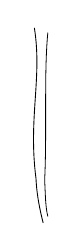
\begin{tikzpicture}[x=1cm,y=1cm,line cap=round]
\draw[line width=.32pt] (0,0) .. controls (.10,-.64) and (-.08,-1.14) .. (.02,-1.91)
 .. controls (.03,-2.14) and (.08,-2.35) .. (.11,-2.47);
\draw[line width=.29pt] (.17,-.06) .. controls (.12,-.59) and (.16,-1.31) .. (.13,-1.93)
 .. controls (.14,-2.13) and (.14,-2.27) .. (.17,-2.39);
\end{tikzpicture}}}
Il faudrait corriger la conj. bordélique dans le cas (\uline{$\overline{\mathrm{III}}$}), en énonçant (sous toutes réserves, encore !) qu'il n'y a (peut-être) pas d'autres scindages de l'ext. $\mathcal{E}$ de $\Gamma$ par $\pi$ que ceux-là ....

\margin{78}

\scanpage{80}
\mspage{38}

10. Ajustement des hypothèses (remords).

Je me rends compte que dans la définition des morphismes $(X',S')\xrightarrow{f}(X,S)$, l'hypothèse $f^{-1}(S)_{\mathrm{red}}=S'$ est étriquée --- il faut prendre des morphismes \uline{quelconques} $f:X'\backslash S'\to X\backslash S$ (se prolongeant bien sûr en $\widehat{f}:X'\to X$).
On aura donc $S'\supset\widehat{f}^{-1}(S)_{\mathrm{red}}$, mais $S'$ peut être strictement plus grand que $\widehat{f}^{-1}(S)_{\mathrm{red}}$.
Il faut alors ajuster en conséquence la description de la ``catégorie bordélique'' --- les objets restent les diagrammes de groupoïdes
\[
\mathcal{D}:\Pi_{D^*}\to\Pi_U\to\Pi_e
\]
(plus donnée de Kummer) mais un morphisme $f$ d'un $\mathcal{D}'$ dans un $\mathcal{D}$ ne définit plus nécessairement un $\Pi'_{D^*}\to\Pi_{D^*}$ (en plus de $\Pi'_U\to\Pi_U$) il faut se donner une partie $I'_f$ de $I'=\pi_0(\Pi'_{D^*})$, et se donner seulement
\[
\Pi'_{D^*,I'_f}\xrightarrow{f_{D^*}}\Pi_{D^*}
\]
(avec donnée de commutation \inserted{$\unsure{\alpha_{D^*U}}$} relatif au carré avec $f_U$).
Bien sûr, dans la description en termes de $\mathcal{E}',\mathcal{E}$ etc., on exige que pour $i'\in I'\backslash I'_f$, $f_{\mathcal{E}}:\mathcal{E}'\to\mathcal{E}$ est trivial sur $\mathcal{E}'_{i'}\subset\mathcal{E}'$ --- et $\tau$ est défini comme $I'_f\to I$ ; \unsure{des|les} données relatives aux $i'\in$

\margin{79}
\scanpage{81}

\(I'_{f'}\quad (f_{i'}:\mathcal E_{i'}\longrightarrow
\mathcal E_{i=\tau(i')},\ \text{les }\alpha_{i'}\in\mathcal E)\)
sont pareils que dans le cas envisagé précédemment.

\uline{NB} Cela signifie en fait qu'on commence \unsure{à} "boucher les trous" \deleted{de}
(de \(X'\)) correspondants aux \(i'\in I'\setminus I'_{f'}\), en remplaçant
\(\mathcal E'\) par le \deleted{\unsure{ss-}}groupe quotient de \(\mathcal E'\)
par le ss-groupe invariant engendré par les
\(L_{i'}=\kappa_{i'}(T(\overline K))\)
\((i'\in I'\setminus I'_{f'})\), et \deleted{les} \unsure{\(\mathcal E_{i'}\)}
\((i'\in I'_{f'})\) par leurs images dans ledit groupe quotient, et en oubliant
\deleted{les} \(I'\setminus I'_{f'}\), i.e. remplaçant \(I'\) par \(I'_{f'}\).

[Pour bien faire, il faudrait exprimer ces opérations aussi au niveau des diagrammes
de groupoïdes
\diagram{\begin{tikzcd}[ampersand replacement=\&]
\Pi'_{\unsure{D^*}} \arrow[r,dash] \& \Pi'_U \arrow[r] \& \unsure{\Pi'_e|\Pi_e}
\end{tikzcd}}
\(\ldots\)].

\margin{\deleted{\illegible{2} il faudrait encore \unsure{expliciter}
\illegible{2} \unsure{des|les} pts de \illegible{1}}}

Cela signifie donc qu'en fait, on s'est ramené à la situation envisagée au début,
où \(S'=\widehat f^{-1}(S)\)\ldots\ Donc finalement
la différence des deux pts de vue n'est pas énorme, et
\deleted{\illegible{1}}\inserted{celui} adopté au début a l'avantage de
la simplicité plus grande (tout est relatif !)

\margin{80}

\scanpage{82}
\mspage{39}

11. Conditions sur les systèmes de \deleted{\unsure{diagrammes}}\inserted{groupoïdes}
obtenus à partir de situations géométriques.

On en a déjà cité au passage, p.ex. que les groupes noyaux de
\(\Pi_{D^*}-\Pi_e\) sont abéliens (avec l'isom de Kummer \(\kappa\))
et que les images sont des sous-groupes ouverts, et de \(=\) pour
l'image des \deleted{\illegible{1}} \(\pi_1\) dans \(\Pi_U-\Pi_e\).
On va réexpliciter \inserted{et préciser} ceci dans le cadre de l'interprétation
en termes de
\diagram{\begin{tikzcd}[ampersand replacement=\&]
T(\overline K) \arrow[r,"\kappa_i"] \& \mathcal E_i \arrow[r,hook,"\rho_i"] \&
\mathcal E \arrow[r,"p"] \& \Gamma
\end{tikzcd}}
(cas de la "dim 1" --- on n'exclut pas le cas \(I=\varnothing\) ---
le cas "dim 0" étant trivial\ldots)

a) L'image \inserted{\(\Sigma\)} de \(p\) est ouverte, plus précisément existe
ss-groupe ouvert \(\Gamma'\subset\Gamma\) au dessus duquel
\(\mathcal E\) ait une section [et = une "section admissible" en un sens qui sera
défini par la suite --- de sorte à exclure les sections "triviales" provenant
des \(\mathcal E_i\)\ldots].

b) L'image \(\Sigma_i\) de \(\mathcal E_i\) dans \(\Gamma\) est ouverte, et
l'extension \(\mathcal E_i\) de \(\Sigma_i\) par \(L_i\)
\((\simeq T(\overline K))\) est triviale. [En fait, on a une classe
\inserted{\uline{privilégiée}} de scindages, dits "algébriques", formant un
torseur sous
\(K_i^*\,\unsure{\hookrightarrow}\,\varprojlim\unsure{(K_i^{*n})_n|(K_i^{*})_n}\),
cf n° 9 \unsure{]|?} --- mais

\margin{81}

\scanpage{83}

on va pas considérer \inserted{pour l'instant} cet élément de structure
supplémentaire\ldots)

\deleted{c) Il faut}

Le reste des \deleted{hypothèses}\inserted{conditions} concerne
essentiellement la structure des groupes \(\pi=\operatorname{Ker}(p:\mathcal E\to\Gamma)\) avec
ses \inserted{classes de conjugaison de} \uline{sous-groupes}
\unsure{(ou plutôt} les hom extérieurs
\(\kappa_i:\deleted{\unsure{\widehat{\mathbb Z}(1)}}T\ (=T(\unsure{\overline K^*}))\longrightarrow\pi\),
et la façon dont \(\Sigma\) opère extérieurement sur \(\pi\).
Ces conditions s'expriment de façon particulièrement simple lorsque les
\(\Sigma_i\subset\Gamma\) sont \(=\Gamma\)
("les pts de \(S\) \inserted{\unsure{tous}} rat / \(K\)") i.e.
\(\mathcal E_i\to\Gamma\) surj., a fortiori \(\Sigma=\Gamma\) i.e.
\(\mathcal E\to\Gamma\) surj. On va se borner à ce cas. Le cas général s'en déduit
par extension finie du corps de base
[\unsure{auquel} \deleted{on les}\inserted{chaque} pts de
\(S\) non rationnels sur \(K\)
\inserted{i.e. chaque \(\Sigma_i\ne\Gamma\)}
\deleted{\unsure{se partagent}\illegible{1}}\inserted{\unsure{donne|donnent} naissance}
à \(n_i\) pts, \deleted{\unsure{ég.}}
\(n_i=[\Gamma:\Sigma_i]\) \unsure{\(\}\)} --- et \(X_{K'}\)
\deleted{\illegible{1}} \unsure{scindé|se scinde} en \(n=(\Gamma:\Sigma)\) comp. connexes
qui sont géom. connexes] --- mais j'ai la flemme d'expliciter comme il faudrait,
dans le contexte des groupoïdes ou des \deleted{\unsure{exten}} hom de groupes
profinis, l'opération d'extension des corps de base\ldots\ Il est entendu que

\margin{82}

\scanpage{84}
\mspage{40}

les conditions que je vais décrire seront invariantes par extension \unsure{du|des} corps de base.

\deleted{c) Il existe \(\unsure{\xi|\zeta}\in T\)
\((=\unsure{T(\overline K^*)})\) et des conjugués}

c) \(\forall i\)\deleted{\illegible{1}}, l'hom extérieur
\[
\kappa_i:T\longrightarrow\pi
\]
est compatible avec l'action extérieure de \(\Gamma\) (opérant sur \(T\) par le
caractère cyclotomique \(\chi\), et sur \(\pi\) grâce à l'extension \(\mathcal E\)
de \(\Gamma\) par \(\pi\)). En d'autres termes, pour \(\forall g\in\mathcal E\),
existe un \uline{\(\alpha\in\pi\)} (\uline{NB} pas seulement
\(\alpha\in\mathcal E\) !) tel qu'on ait,
\[
\operatorname{int}(g)\kappa_i(\unsure{\xi|\zeta})
=\operatorname{int}(\alpha)\kappa_i(\chi(p(g))\unsure{\xi|\zeta})
\]
i.e.
\[
\operatorname{int}(\alpha^{-1}g)\kappa_i(\unsure{\xi|\zeta})
=\kappa_i(\chi(p(g))\unsure{\xi|\zeta})
\]
Ceci signifie donc que 1°) \(\alpha^{-1}g\) normalise \(L_i=\kappa_i(T)\).
[et cela signifie \(=\), probablement, que \(\alpha^{-1}g\in\mathcal E_i\)
--- et qu'on puisse trouver un tel \(\alpha\in\pi\)
\inserted{tel que \(\alpha^{-1}g\in\mathcal E_i\)} provient de l'hypothèse
\(\mathcal E_i\to\Gamma\) surjectif --- on prend un \(\beta\in\mathcal E_i\)
\inserted{\(\unsure{=}\alpha^{-1}g\)} ayant \(=\) image que \(g\) dans \(\Gamma\)
et on prend \(\alpha=g\beta^{-1}\)] et que 2°) l'action \inserted{intérieure} de
\(\beta=\alpha^{-1}g\) sur \(T\) n'est autre que par multiplication
par \(\chi(g)=\chi(\beta)\) --- ce qui (pour \(\beta\in\mathcal E_i\)) n'est autre que la

\margin{83}

\scanpage{85}

condition déjà explicitée que l'hom de groupes \(\kappa_i:T\to\mathcal E_i\)
est compatible avec l'action de \(\mathcal E_i\), opérant sur \(T\) via
\(\chi\circ p\mid\mathcal E_i\), et sur lui-= par autom. int.

Donc la condition c) n'est pas vraiment nouvelle --- je la réexplicite en termes
un peu différents, à cause de son importance. Elle implique que l'opération
\margin{\figure{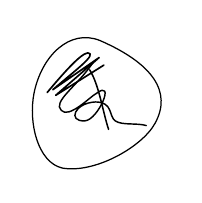
\begin{tikzpicture}[x=.012cm,y=-.012cm,line cap=round,line join=round]
\draw[line width=.45pt] (105,61) .. controls (73,48) and (43,77) .. (35,117)
 .. controls (29,148) and (39,190) .. (65,196)
 .. controls (99,202) and (149,174) .. (163,149)
 .. controls (182,115) and (160,85) .. (105,61);
\draw[line width=.52pt] (97,85) .. controls (81,109) and (54,126) .. (64,135)
 .. controls (72,144) and (95,120) .. (101,117)
 .. controls (122,101) and (103,145) .. (89,146)
 .. controls (70,147) and (78,127) .. (100,126)
 .. controls (119,126) and (114,141) .. (121,146)
 .. controls (128,151) and (144,148) .. (154,151);
\draw[line width=.55pt] (94,92) .. controls (104,108) and (108,137) .. (114,155);
\draw[line width=.60pt] (49,116) .. controls (65,97) and (84,75) .. (92,74)
 .. controls (103,75) and (78,93) .. (55,113)
 -- (104,79) -- (58,119) -- (109,87);
\end{tikzpicture}}}
de \(\Gamma\) sur \(\pi\) est \uline{très} non triviale (puisque
\(\chi:\Gamma\to\widehat{\mathbb Z}^{*}\) a une image ouverte !)
--- il \unsure{n'était} pas \(=\) évident a priori
\inserted{(sans raisons arithmétiques profondes !)} --- compte tenu de la structure
de \(\pi\) qu'on va donner --- qu'il existe de telles opérations de \(\Gamma\)
sur un \(\pi\) !

Cette condition \unsure{sera} complétée par une condition de non-trivialité à la Weil.

d) \(\exists\eta\in T^*\)\unsure{.} (une base de \(T\)), et des
\(\alpha_i\in\pi\) (afin de conjuguer \(\kappa_i\) en
\(\kappa'_i=\operatorname{int}(\alpha_i)\circ\kappa_i\))
\unsure{enfin} un entier \(g\geq0\) et des éléments
\(\unsure{x_i,y_i}\in\pi\) \((1\leq i\leq g)\), tels que l'on ait

\margin{84}

\scanpage{86}
\mspage{41}

1°) les \(\kappa'_i(\eta)\), \deleted{\illegible{1}} et les
\(\unsure{x_i,y_i|x_j,y_j}\) engendrent le groupe profini \(\pi\)

2°) Ils satisfont la relation
\[
\boxed{[x_1,y_1].[x_2,y_2]\ldots[x_g,y_g]\,
\kappa'_1(\eta)\kappa'_2(\eta)\ldots\kappa'_{\unsure{\nu|n}}(\eta)=1}
\]

3°) Cette relation, avec les générateurs envisagés décrit \(\pi\)
\inserted{(en tant que groupe profini)} par générateurs et relations\ldots

\uline{NB} On sait que par ces conditions, \(g\) est uniquement déterminé,
p.ex. par le fait que
\(\pi_{ab}/\deleted{\text{images des}}\sum\kappa_i(T)\)
est un \(\widehat{\mathbb Z}\)-module libre de rang \(2g\) --- \(\pi_{ab}\)
étant libre de rang \(2g+\nu-1\) où \(\nu=\operatorname{card}(I)\).

Pour le choix de \(\eta\), on sait que si \(\eta\) convient, alors
\(\forall\ \chi(\alpha)\eta\) aussi (où \(\alpha\in\Gamma\)) --- quitte à prendre
des conjugués. Donc les \(\eta\) qui conviennent \deleted{forment} contiennent
un sous-torseur\inserted{de \(T^*\)} (sous le ss-groupe ouvert
\(\chi(\Gamma)\) de \(\widehat{\mathbb Z}^{*}\).

\deleted{Supposons pour simplifier que \(g=0\) :
On voit donc que si le système des \(\kappa'_i(\eta)\) est un syst. de gén.
privilégié (au sens de d) ci-dessus) alors les
\(\operatorname{int}(g)\kappa'_i(\eta)\) aussi pour \(\forall g\in\mathcal E\),
[\unsure{\(=\)} \(\operatorname{int}(\alpha)\kappa'_i(\chi(g)\eta)\)
pour \(\alpha\in\pi\) convenable]}

\margin{85}

\scanpage{87}
\mspage{42}

\margin{(\unsure{donc|dans} \(\chi:\Gamma\to\widehat{\mathbb Z}^{*}\) \unsure{épi.})}

\deleted{donc aussi les \(\kappa'_i(\chi(g)\eta)\). \unsure{Prenant}
\(K=\mathbb Q\), on trouve donc par voie arithmétique :

\uline{Prop} Soit \(\pi\) le \unsure{\(P\)}-groupe libre
\inserted{de \unsure{\(\nu-1\)|\(\nu\) gén.}} \unsure{(}\uline{engendré} par des générateurs
\(\ell_1,\ldots,\ell_\nu\) satisfaisant la relation génératrice
\(\prod\ell_i=1\). Alors pour tout \(\alpha\in\widehat{\mathbb Z}^{*}\),
on a encore \(\prod\ell_i^\alpha=1\), et les \(\ell'_i=\ell_i^\alpha\)
avec cette relation décrivent le groupe profini \(\pi\).}
En fait, comme la structure du groupe \(\pi\) est indépendante de \(K\),
prenant \(K=\mathbb Q\) (et admettant qu'il existe une courbe lisse projective
géom. connexe de genre \(g\) sur \(\mathbb Q\), ayant \(\nu\) pts rat. / \(\mathbb Q\) !),
on trouve que si les \(\ell_i\), \deleted{\(\unsure{x_j,y_j}\)}
\((1\leq i\leq\nu\deleted{,\ \unsure{1\leq j\leq g}})\)
\deleted{conviennent, alors les} s'insèrent dans un syst. de générateurs
privilégié (avec des \(\unsure{x_\alpha,y_\alpha}\)) alors pour
\(\forall\rho\in\widehat{\mathbb Z}^{*}\), on peut trouver des conjugués
\(\ell'_i\) des \(\ell_i^\rho\) qui s'insèrent de \(=\).
Même pour \(\rho=-1\) ce n'est pas entièrement trivial\ldots

\deleted{\illegible{2}} Enfin, \unsure{on va} énoncer une condition
draconienne de non trivialité de l'opération de \(\Gamma\) sur \(\pi\).
Soit \(\mathcal E'\) un sous-groupe \inserted{\uline{ouvert} (donc}
d'indice fini) de \(\mathcal E\),
\inserted{\(\pi'=\pi\cap\mathcal E'=\operatorname{Ker}(\mathcal E'\to\Gamma')\)}
\deleted{\illegible{1} son image dans \unsure{\(\mathcal E\)|\(\Gamma\)}
(qui est ouvert dans \(\Sigma\)) de sorte que}

\margin{86}

\scanpage{88}

\(\Gamma'\) l'image de \(\mathcal E'\) dans \(\Gamma\). On trouve donc une
extension de \(\Gamma'\) \((=\operatorname{Gal}(\overline K'/K'))\) sur \(\pi'\),
donc aussi par \(\unsure{(\pi'_{ab})_{(\ell)}}\)
(\(\ell\) étant un nb premier), qui est (on le sait par d)) un
\(\mathbb Z_\ell\)-module libre de t.f.,
\inserted{sur lequel \(\Gamma'\) opère}

[Avec un peu de travail, on doit pouvoir mettre sur
\(\mathcal E'\to\Gamma\) une "structure à lacets" i.e. des
\(\mathcal E'_{i'}\), comme pour \(\mathcal E\), et décrire dans
\(\unsure{(\pi'_{ab})_{(\ell)}}\)
\inserted{la somme} des images des \deleted{\illegible{1}} \(L'_{i'}\),
sur lesquels \(\Gamma'\) opère \inserted{donc} via le caractère \(\chi\).

\margin{Ça se fait très élégamment dans le contexte
\diagram{\begin{tikzcd}[ampersand replacement=\&]
\Pi_{D^*} \arrow[r] \& \Pi_U \arrow[r] \& \Pi_e
\end{tikzcd}}}

On s'intéresse au quotient de \(\unsure{(\pi'_{ab})_{(\ell)}}\) par
\unsure{ce sous-module|ces sous-modules} relativement trivial (la partie "VA" du
module \(\ell\)-adique envisagé). Ceci posé

\textcircled{e} on exige que la représentation de \(\Gamma'\) là dessus soit
"pure de poids 1" --- \deleted{\unsure{i.e.} on ait} et que les polynômes car.
des frobénius (qui sont à coefficients \(\in\mathbb Z\), pas seulement
\(\in\mathbb Z_\ell\)) soient \uuline{indépendants} de \(\ell\).

\margin{\figure{\begin{tikzpicture}[x=1cm,y=1cm,line cap=round]
\draw[line width=.34pt] (.04,.30) .. controls (-.30,.35) and (-.42,.13) .. (-.40,-.08)
 .. controls (-.39,-.36) and (-.14,-.39) .. (.08,-.23)
 .. controls (.36,-.01) and (.28,.27) .. (.04,.30);
\node[inner sep=0pt] at (-.08,-.02) {$e$};
\draw[line width=.29pt] (-.06,-.71) .. controls (.01,-1.68) and (-.08,-2.52) .. (.02,-3.52)
 .. controls (.09,-4.37) and (.08,-5.24) .. (.15,-5.98)
 -- (.07,-6.30);
\end{tikzpicture}}}
\margin{87}

\scanpage{89}
\mspage{43}

12. \uline{L'analogie topologique}

Soit \(X\) une \deleted{variété}\inserted{surface} (topologique) compacte
orientable, \(S\) une partie finie de \(X\). Si \(X\) est connexe, on considère
l'ensemble \inserted{\unsure{\(\omega\)}} \unsure{des|ses} deux orientations,
on l'utilise pour tordre le groupe \(\mathbb Z\), d'où un groupe \unsure{\(T\)}
\[
T=\mathbb Z\mathop{\wedge}\limits_{\pm1}\unsure{\{\omega\}|\omega}.
\]
isomorphe (non canoniquement) à \(\mathbb Z\). Plus généralement, supposons
donné un tel groupe \(T\),
\inserted{i.e. un \(\omega\in\unsure{\operatorname{Ob}}\mathrm{Ens}_2\)}
--- une \(T\)-orientation de \(X\) sera par définition un \unsure{élém.}
de l'ens. \(\operatorname{Or}(X)\mathop{\wedge}\limits_{\{\pm1\}}\omega\).

[dans le cas précédent, \(X\) sera donc canoniquement \(T\)-orienté\ldots]

Considérons le groupoïde fondamental de \(X\setminus S=U\), soit \(\Pi_U\),
et le groupoïde fondamental \inserted{\(\Pi_{D^*}\)} des germes
d'espaces de \(X\) autour de \(S\), \uline{privé} de \(S\)
\inserted{\deleted{\unsure{des}} groupoïdes \unsure{?}}
(des germes de rev. universels de \(X\setminus S\) au voisinage de \(S\)).
On a donc un foncteur canonique
\diagram{\begin{tikzcd}[ampersand replacement=\&]
\unsure{\Pi_{D^*}} \arrow[r,dash] \& \Pi_U
\end{tikzcd}}
et d'autre part, \deleted{\illegible{2}} si \(X\) est \(T\)-orienté, on a une
structure supplémentaire

\margin{88}

\scanpage{90}

intéressante sur \inserted{le groupoïde} \(\Pi_{D^*}\) : le système local de
ses \(\pi_1\) est can. isom. à \(T\).

Associant à tout \(X\) \(T\)-orienté le système
\[
\Pi_{D^*}\longrightarrow\Pi_{\unsure{X|U}},\qquad
\kappa:T_{(\Pi_{D^*})}\simeq\pi_1(\Pi_{D^*}/e),
\]
on trouve une 2-équivalence entre la 2 catégorie topologique des
\deleted{\unsure{variétés}} couples \((X,S)\) d'une
\inserted{(pour les homéo. à isotopie près\ldots)}
\unsure{variété compacte \(T\)-orientée}, et de la 2-catégorie des systèmes
précédents \inserted{(pour les équivalences)}, \unsure{(}qui satisfont les conditions

a) \(\pi_0(\Pi_{D^*})\), \deleted{\unsure{et}} \(\pi_0(\Pi_X)\) finis

b) Pour \unsure{tte|\(\forall\)} composante connexe de \(\Pi_U\), soit
\(\Pi_{U_0}\), et la partie \(\unsure{\Pi_{D_0^*}}\) au dessus, explicitant la
situation \unsure{groupoïdes} par \unsure{un|une}
\inserted{groupe \(\pi\) et une} famille d'homs
\(T\xrightarrow{\kappa_i}\pi\), on a (\uline{NB} le tout \unsure{dépend|dépendant} de choix,
mais \(\pi\) est intrinsèque comme groupe extérieur, et les \(\kappa_i\)
\unsure{comme homs} extérieurs --- \unsure{définissent|définissant} une "\(T\)-structure à lacets
sur \(\unsure{S}\) ---) on a ce qui suit.

\margin{89}
\scanpage{91}
\mspage{44}

$\exists$ générateur $g\in T$ (i.e. $g\in T^*$) et un ordre \inserted{$i_1$--$i_\nu$}
sur l'ens. $I$, \deleted{\illegible{2}} des conjugués
$\unsure{l_i'|l_{i_\alpha}'}$ des $\kappa_{i_\alpha}(g)$, et $g\in\mathbb N$ et des $x_\alpha,y_\alpha\in\pi$
$(1\leq\alpha\leq g)$ tels que l'on ait
\[
\left(\prod_1^g[x_\alpha,y_\alpha]\right)\prod_1^{\nu}l_i=1
\]
et que ceci soit une relation de définition
de $\pi$.

Il y a \inserted{cependant} un grain de sel pour $I=\varnothing$
(auquel cas $T$ ne sert à rien \inserted{apparemment} (dans la
description groupoïdale de $(X,S)$ \unsure{$\simeq$|$=$} $(X,\varnothing)=X$)
il faut alors, \unsure{\deleted{au}} lieu des données
``kummériennes'' \inserted{$\kappa$}, se donner
\[
H^2(\pi,\mathbb Z)\overset{\kappa}{\simeq}T
\]
\margin{Il faut introduire \inserted{\unsure{donc}} \unsure{ceci} comme donnée supplémentaire,
dans la définition des groupes à lacets l'exclusion des cas $X_0\simeq S^2$ (dans le cas $S$ vide) est \unsure{alors} particulièrement \unsure{convaincante}.}

Enfin, il faut \deleted{\illegible{1}}
(\unsure{$\bar{\mathrm m}$|$=$} avec ce grain de sel) exclure le cas $X=S^2$, $S=\varnothing$
(en tant que comp. connexe) --- i.e.
du côté groupes, le cas d'une \inserted{comp. de $\Pi_U$ où}
$\pi=(1)$ \deleted{\illegible{2} $I=\varnothing$} et $I=\varnothing$.
[Si je me rappelle bien, il n'y a pas lieu
d'exclure $(S^2,\mathrm{pt})$ (i.e. $X\setminus S=U\simeq\mathbb R^2\simeq\mathbb E^1_{\unsure{\mathbb C|e}}$)
\margin{90}

\scanpage{92}

où pourtant \unsure{on a} $\pi=0$. Mais sauf dans ces
deux cas, \deleted{les hom. $\kappa_i:$} (correspondant
au cas $g=0$, $\nu=1$) l'hom. $\kappa_i:T\longrightarrow\pi$
est injectif. Si $T=\mathbb Z$ la donnée des $\kappa_i$
équivaut à celle d'éléments $l_i\in\pi$, et on
retrouve la définition usuelle des
structures à lacets.

Ceci est explicité dans la thèse de
Yves Ladegaillerie --- ce qui y manque, est
(entre autres) la considération de flèches
entre $(X,S)$ autres que des homéomorphismes
(mod isotopies)\,; p.ex. des applications \deleted{étales}
\deleted{\illegible{3}} $X'\xrightarrow{f}X$ telles que $S'=f^{-1}(S)$
[et que $X'$ soit étale sur $X\setminus S$, si on y tient\unsure{!}],
ce qui se ramène au cas précédent
--- le cas \inserted{plus} général où on suppose seule-
ment que $X'$ est un rev. ramifié
de $X$ (pouvant être ramifié aussi en
dehors de $S'$) et $S'\supset f^{-1}(S)$ (mais $S'$
pouvant être plus grand) demanderait
\margin{91}

\scanpage{93}
\mspage{45}

une étude soigneuse, avec une notion
ad-hoc de l'isotopie ....

Une autre direction importante (notam-
ment pour l'étude \unsure{du|des} cas non orienté,
non orientable) est l'introduction des
groupes finis d'homéomorphismes, ne
respectant pas nécessairement l'orientation.
Pour traiter le cas du changement d'orientation,
notons que dans la description groupoïdale
$(\Pi_{D^*}\longrightarrow\Pi_U,\kappa)$ d'une $(X,S)$ $T$-orientée,
le passage à l'orientation opposée s'exprime en
gardant tel quel $\Pi_{D^*}\longrightarrow\Pi_U$, et en
remplaçant $\kappa$ par $\bar\kappa=\kappa^{-1}$
\[
\bar\kappa(\unsure{\zeta|\xi})=\kappa(-\unsure{\zeta|\xi})=\kappa(\unsure{\zeta|\xi})^{-1}
\]
(Si \inserted{$T=\mathbb Z$, sur} le système $(\pi,(l_i))$, cela revient à
remplacer les $l_i$ par les $l_i^{-1}$ ...)
\margin{et itou (si $I=\varnothing$) pour $\kappa:T\simeq H^2(\pi,\mathbb Z)$
\unsure{remplacé} par $-\kappa$.}

Soit donc $\Gamma$ un groupe (a priori
\unsure{pas} néc. fini) qui opère sur $(X,S)$, donc
sur $U=X\setminus S$ \inserted{et sur $\Pi_U$, $\Pi_{D^*}$.} On trouve alors des
groupoïdes \inserted{fondamentaux} mixtes \deleted{\illegible{1}} par la construction bien connue
\margin{92}

\scanpage{94}

\diagram{\begin{tikzcd}[ampersand replacement=\&]
\Pi_{D^*,\Gamma} \arrow[r] \& \Pi_{U,\Gamma} \arrow[r] \& \Pi_{e,\Gamma}
\end{tikzcd}}
catégorie des $\Gamma$-torseurs
i.e. des objets $1$-connexes
dans $\Gamma$-Ens

correspondant aux foncteurs en sens inverse

\diagram{\begin{tikzcd}[ampersand replacement=\&]
\text{$\Gamma$-rev. \unsure{étale|étales} de $D^*$} \& \text{$\Gamma$-rev. \unsure{étale|étales} de $U$} \arrow[l] \& \text{$\Gamma$-Ens.} \arrow[l]
\end{tikzcd}}

Les comp. connexes de $\Pi_{D^*,\Gamma}$ correspondent
aux \uline{orbites de $\Gamma$ dans $S$} \deleted{\illegible{1}} $\simeq\pi_0(\Pi_{D^*})$,
de même pour celles de $\Pi_{U,\Gamma}$. Le \deleted{\unsure{top.}}
$\Pi_{U,\Gamma}$ connexe \inserted{i.e. le topos $\widehat\Pi_{U,\Gamma}$ connexe,}
est celui \unsure{où|à} $\Gamma$ transitif
sur $\pi_0(U)\simeq\pi_0(X)$ --- quitte à remplacer
$X$ par une composante connexe $X_0$, et $\Gamma$
par le \unsure{s.-s.-groupe|sous-groupe} $\Sigma\subset\Gamma$ qui la stabilise,
on serait ramené (pour l'étude des
topos $\widehat\Pi_{U,\Gamma}$ et des morphismes de topos
\diagram{\begin{tikzcd}[ampersand replacement=\&]
\widehat\Pi_{D^*,\Gamma} \arrow[r,dash] \& \widehat\Pi_{U,\Gamma} \arrow[r] \& (\unsure{\widehat\Pi_{e,\Sigma}} \arrow[r] \& )\widehat\Pi_{e,\Gamma}
\end{tikzcd}}
au cas de $(X_0,S_0,\Sigma)$. Mais \unsure{l'analogie|l'analogue}
\margin{93}

\scanpage{95}
\mspage{46}

que j'ai en vue avec le cas ``arithmétique''
rend cette réduction inopportune dans le
cas général (car dans le \unsure{\deleted{cas}} arithmétique,
on ne se borne pas non plus au cas où
$\Sigma=\Gamma$ i.e. $\mathcal E\longrightarrow\Gamma$ surjectif, i.e. \inserted{la comp. connexe}
$X$ \uline{géométrique-}
\uline{ment} connexe sur $K$). Notons \inserted{ici} que
$(X,S,\Gamma)$ se récupère à partir des
$(X_0,S_0,\Gamma_0=\Sigma)$ comme somme amalgamée
\[
X=X_0\,\unsure{\wedge|\widehat\times}_{\Sigma}\Gamma\quad ....
\]

Quand on exprime (pour $\Pi_{\unsure{U|X},\Gamma}$ connexe)
la situation en termes de théorie des groupes,
on trouve donc \deleted{\illegible{1}} un groupe
fondamental \deleted{$\mathcal E_X$} mixte
\[
\mathcal E_{\unsure{U|X},\Gamma}=\pi_1(U,\Gamma)
\]
et un hom.
\[
\mathcal E_{U,\Gamma}\longrightarrow\Gamma
\]
--- (Surjectif ssi. \deleted{$\Gamma$ transitif sur $\pi_0(U)=\unsure{\Gamma/\Sigma}$}
\inserted{$U$ connexe (on a $\Gamma/\Sigma\simeq\pi_0(U)$)})
\inserted{enfin un ens. d'indices}
\deleted{correspondant à \illegible{1} $\pi_0(U)/\Gamma$}
$I$ ($\simeq\unsure{S}/\Gamma\simeq\pi_0(\Pi_{D^*,\Gamma})$) et des
groupes fondamentaux mixtes
\margin{94}

\scanpage{96}

\[
\mathcal E_i\xrightarrow{\sim}\unsure{\pi_1|\Pi_1}(D_i^*,\Gamma)
\simeq\pi_1(D_{i_0}^*,\unsure{\Sigma_{i_0}|\Gamma_{i_0}})
\]
où $D_{i_0}^*$ est une composante connexe du
multidisque troué $D_i^*$ \inserted{(correspondant au choix d'un $\unsure{s_i}\in S$)}, et où $\unsure{\Sigma_{i_0}|\Gamma_{i_0}}\subset\Gamma$ est
son stabilisateur (i.e. le stabilisateur de
$s_i$ dans $\Gamma$), qui est \deleted{\unsure{un gr.}} (si $\Gamma_i$ \inserted{est fini et} opère
fidèlement au voisinage de $s_i$) un groupe cyclique
ou dihédral ... On trouve donc, si $X$ est
$T$ \unsure{orienté|orientée}, une extension de $\Gamma_{i_0}$ par $T$,
l'hom. $\mathcal E_i\longrightarrow\unsure{\Sigma_{i_0}|\Gamma_{i_0}}\subset\unsure{\Gamma|\Gamma_i}$ étant induit
bien sûr via $\mathcal E_{U,\Gamma}\longrightarrow\Gamma$ et $\mathcal E_i\longrightarrow\mathcal E_{U,\Gamma}$.

Il faut \inserted{encore} lier l'action de $\Gamma$ sur $X$ à
l'orientation de $X$ --- pour ceci on suppose
donné un caractère
\[
\chi:\Gamma\longrightarrow\mathbb Z^*=\{\pm1\}
\]
et on exige que pour $g\in\Gamma$, $g_X$ \unsure{conserve}
l'orientation si $\chi(g)=1$, la renverse si $\chi(g)=-1$.
Ceci implique que \deleted{\unsure{l'}}\inserted{\unsure{l'on a un|l'hom. ou}} isomorphisme
\[
\pi_1(\Pi_{D^*,\Gamma}/\Pi_{\unsure{e},\Gamma})
\overset{\kappa_\Gamma}{\xleftarrow{\sim}}T
\]
\margin{système local des noyaux des
$\pi_1(\xi)\longrightarrow\pi_1(\varphi p(\xi))$
pour $\xi\in\operatorname{Ob}\Pi_{D^*,\Gamma}$.}
\margin{95}

\scanpage{97}
\mspage{47}

$T$ étant considéré comme système local
sur $\Pi_{\Gamma,e}$ \deleted{\illegible{1}} i.e. comme $\Gamma$-groupe, grâce à l'action
de $\Gamma$ via le caractère $\chi$. Il revient au
même de dire que \inserted{$\forall i\in I$} l'application
\deleted{La donnée}
\[
\kappa_i:T\xrightarrow{\sim}L_i=\operatorname{Ker}(\mathcal E_i\longrightarrow\Gamma)
\]
en tant que hom. de $T$ dans $\mathcal E_i$ est
compatible avec l'action de $\mathcal E_i$ (opérant
sur $T$ via $\chi p_i$ ($p_i:\mathcal E_i\longrightarrow\Gamma$)), \illegible{1} et sur
lui-= par autom\unsure{s}. int ...

Si on exclut le cas où $(X_0,\unsure{S_0})$
est $\simeq(S^2,\varnothing)$ ou $(S^2,1\ \mathrm{pt})$ (i.e.
le cas $\pi=0$), les $\kappa_i:T\longrightarrow\pi$ sont injectifs,
donc aussi les $\mathcal E_i\longrightarrow\mathcal E_{U,\Gamma}$, donc les
$\mathcal E_i$ peuvent être considérés comme des
\uline{sous-groupes} de $\mathcal E_{U,\Gamma}$.

\unsure{\S} Ici il \deleted{\illegible{1}} serait particulièrement
contre-indiqué (\unsure{$\bar{\mathrm m}$|$=$} si on suppose $\Sigma=\Gamma$ i.e.
$X=X_0$ i.e. $X$ connexe) de supposer que
les $\Gamma_i$ \unsure{soit|sont} $=\Gamma$ i.e. que les $s\in S$ sont fixes
par $\Gamma$ !
\margin{96}

\scanpage{98}

Comme le centre de $\pi$ est \deleted{\illegible{1}}réduit à $1$
(si on excepte \deleted{\unsure{resp.}} le cas $(X_0,S_0)\simeq(S^2,\text{deux pts})$
i.e. $U_0\simeq\mathbb C^*$ \inserted{--- cas de la couronne ---}), la donnée d'une extension
de $\Sigma$ ($\subset\Gamma$) par $\pi$ revient (à \unsure{isom.} unique
près) à la donnée d'un hom.
\[
\unsure{\Sigma|\Gamma}\longrightarrow\mathrm{Aut\,ext}(\pi)\quad\deleted{\text{structure à lacets}}
\]
\deleted{de $\Sigma$ dans le ``groupe de Teichmüller''
relatif à $\pi$ ($\simeq\pi_1(X_0)$)} --- $\mathcal E$ se reconsti-
tue comme l'image inverse de l'extension
\diagram{\begin{tikzcd}[ampersand replacement=\&]
1 \arrow[r] \& \pi \arrow[r] \& \mathrm{Aut}(\pi) \arrow[r] \& \mathrm{Autext}\,\pi \arrow[r] \& 1
\end{tikzcd}}.

Mais ici les \unsure{automs} extérieurs relatifs
aux $\alpha\in\Sigma$ \deleted{envisagés sont} \uline{respectent la structure}
à lacets \deleted{\illegible{1}} de $\pi$, modulo le
signe $\chi(\alpha)$ --- i.e. pour $g\in\mathcal E$, et $s\in S$
$\exists\ \alpha\in\pi$ \inserted{et $s'\in S$ ($s'$ unique !)} tels que
\[
\deleted{\unsure{\varphi|g}}\quad
\operatorname{int}(g)\kappa_s(\unsure{\zeta|\xi})
=\operatorname{int}(\alpha)\kappa_{s'}(\chi(p(g))\unsure{\zeta|\xi})
\]
$\forall\unsure{\zeta|\xi}\in\unsure{T|\mathbb Z}$, i.e.
\[
\operatorname{int}(\alpha^{-1}g)\kappa_s(\unsure{\zeta|\xi})
=\deleted{\unsure{\chi}}\unsure{\kappa_i|\kappa_{s'}}(\chi(p(g))\unsure{\zeta|\xi})
\]
\deleted{ce qui implique que $\alpha^{-1}g$ normalise $L_s=\kappa_s(T)$}
\margin{97}

\scanpage{99}
\mspage{48}

\deleted{(donc sans doute $\alpha^{-1}g\in\mathcal E_s$ ?), et y
opère \illegible{2}}
Ainsi, l'opération de
$\Sigma$ sur $S_0$ (donc de $\Gamma$ sur $S=S_0\wedge_{\Sigma}\Gamma$)
est connue, par l'opération ext. de $\Sigma\subset\Gamma$ sur
$\pi$ munie de sa structure \deleted{\illegible{1}} à
``$T$-lacets'' (i.e. les hom. extérieurs
$\kappa_s:T\longrightarrow\pi$) --- donc aussi $I=S_0/\Sigma\simeq S/\Gamma$.

Peut-on reconstituer $\mathcal E_i$ \inserted{($i\in I$)} à partir de la
\deleted{\unsure{si} $i=s\bmod\Sigma$}
structure d'extension ? On voit, \deleted{que}
\deleted{$\mathcal E_{i_0}\subset\operatorname{Norm}_{\mathcal E}(L_s)$}
en vertu des choix faits,
que si $i\in I$ (donc $i$ une orbite de
$\Sigma$ dans $S_0$) $\exists\ s\in i$ tel que $\operatorname{Ker}(\mathcal E_i\longrightarrow\Gamma)$
ne soit autre que $L_s=\kappa_s(T)$, et on a
donc $\mathcal E_i\subset\operatorname{Norm}_{\mathcal E}(L_s)$, Mais
on a
\[
\operatorname{Norm}_{\mathcal E}(L_s)\cap\pi
=\operatorname{Norm}_{\pi}(L_s)=L_s
\]
$\unsure{=|\ne}\mathcal E_i\cap\pi$, et d'autre part l'image de
$\operatorname{Norm}_{\mathcal E}(L_s)$ dans $\Sigma\subset\Gamma$ n'est \deleted{autre que} \inserted{$\subset$}
$\Sigma_s=$ stabilisateur \deleted{de} \inserted{$s$ dans} $\Sigma$
$=$ Image de $\mathcal E_i$ dans $\Sigma$,
\unsure{et|donc} en résumé
\[
\mathcal E_i=\operatorname{Norm}_{\mathcal E}(L_s)
\]
\margin{98}

\scanpage{100}

Inversement, la donnée de $\mathcal E\longrightarrow\Gamma$
et des $\mathcal E_i$, $\kappa_i:T\longrightarrow\mathcal E_i$ redonne la
structure à lacets de $\pi$, en prenant
les $\kappa_i$ et tous leurs conjugués exté-
rieurs \inserted{distincts} par les $\alpha\in\Sigma$ (modifiés par $\chi(\alpha)$ ...).
Donc la \inserted{donnée de la} situation $\mathcal E\xrightarrow{p}\Gamma$, $\mathcal E_i\subset\mathcal E$
\deleted{équivalent} (famille de ss-groupes, chacun
\unsure{défin.} mod conjugaison \uline{dans $\mathcal E$}) équivaut
à la donnée de

a) $\pi=\operatorname{Ker}p$, avec sa structure à \inserted{$T$-}lacets
(\deleted{famille finie de \unsure{classes de conj.}}\inserted{ens. fini d'hom. extérieurs de}
$T$ dans $\pi$)

b) Un \unsure{sous-}\deleted{groupe} groupe $\Sigma\subset\Gamma$, et
un hom.
\[
\Sigma\longrightarrow\text{Teichmüller étendu de }\pi
\]
(autom. extérieurs de $\pi$,
respectant la structure à lacets
modulo signe
compatible avec le caractère $\chi|\Sigma$ et
le caractère ``signe'' sur Teichmüller étendu.
En fait, $(X,S,\Gamma)$, ou $(U,\Gamma)$, ne définit
$\pi$ que comme groupe extérieur \inserted{à $T$-lacets} sur lequel
$\Gamma$ opère de façon compatible avec $\chi$.
\margin{99}
\scanpage{101}
\mspage{49}
% Main text, approximately lines 1--2.
En résumé, on a un foncteur \deleted{\illegible{1}}\inserted{canonique}
% Approximately lines 3--10; the source of the vertical functor.
Cat. isotopique des \((X,S,\Gamma)\), \(X\) surface compacte \deleted{\illegible{1}},
\(T\) orienté, \(S\) partie discrète, \(\Gamma\) opérant par \unsure{\(\chi\)-autom.}
(\inserted{\(\sigma\in\Gamma\)}\unsure{respectant|respecte} l'orientation si \(\chi(\sigma)=+1\), la renversant
si \(\chi(g)=-1\)), \(\Gamma\) transitif sur \(\Pi_0(X)\),
\deleted{\illegible{1}} et si \((X_0,S_0)\) est une composante connexe
de \((X,S)\), on veut que \deleted{\((X_0,S_0)\) \illegible{2}}\inserted{si \(X_0\simeq S^2\), on}
ait \(\operatorname{card} S_{\unsure{0}}\geq 3\) \deleted{\illegible{3}}.
% Under "ait card S ≥ 3" a smaller line of text is struck through by one long stroke;
% "ait" itself is neither underlined nor struck.
\deleted{\illegible{1} \unsure{isom.}}
\margin{flèches : \unsure{classes} d'isotopie d'homéom. respect. toutes les structures.}

\diagram{\begin{tikzcd}[row sep=2.5em]
{} \arrow[d] \\
{}
\end{tikzcd}}

% Approximately lines 11--18.
Catégorie des groupes extérieurs à \inserted{\(T\)-}lacets \(\pi\),
\inserted{\(\pi\) non commutatif (i.e. \(\pi\neq 0,\mathbb Z\));}
sur lesquels un sous-groupe \(\Sigma\subset\Gamma\) de \(\Gamma\) \inserted{opère}
(cette description étant
équivalente : une description en termes
de systèmes de groupoïdes
\[
\Pi_{\unsure{D^*},\Gamma}\longrightarrow\Pi_{U,\Gamma}
\longrightarrow\Pi_{e,\Gamma}\quad\text{et }\kappa\ldots,
\]
plus conceptuelle dans certains contextes\ldots).
% Long oblique note in the left margin beside the target category.
\margin{Attention \unsure{au} cas \(S=\varnothing\) dans la définition des structures : \unsure{la} \illegible{1} (donnée de
\(H^2(\pi,\mathbb Z)\overset{\kappa}{\simeq}T\)); il faut bien sûr tenir compte \unsure{lors de} l'action de \(\Sigma\) sur
\(H^2(\pi,\mathbb Z)\) \deleted{\unsure{et sur \(T\)}}
(via son action ext. sur \(\pi\)) et sur \(T\) (via \(\chi\)) et \unsure{exiger la} compatibilité.}

% Approximately lines 19--25; the sentence continues on scan 102.
\deleted{\unsure{Pour déf.}} Je présume que la démonstration
\unsure{du} fait que ce foncteur soit pl. fidèle
ne fasse pas de difficultés essentielles,
% Oblique note in the lower-left margin, tied by a double bar and an arrow to the three preceding lines.
\margin{Ça vaudrait drôlement le coup de le faire très soigneusement\ldots}
en utilisant ce qui est connu pour
\(\Gamma=1\). Mais le fait que, \unsure{pour|\deleted{pour}} \(\Gamma\) groupe
fini donné, \deleted{\unsure{qu'il soit un isomorp.}}\inserted{il soit \unsure{ess\textsuperscript{t}} surjectif}
% Lower-left handwritten pagination; attribution of this numbering is uncertain.
\margin{100}

\scanpage{102}
% Approximately lines 1--7; continuation from scan 101.
est un problème ouvert sur lequel les
gens sèchent. Bien sûr OPS \(\Sigma=\Gamma\),
\inserted{et \(\Gamma\subset\) Teichmüller étendu}
et la question est si tt sous-groupe
fini du Teichmüller étendu se
réalise comme groupe opérant sur \((X_0,S_0)\) \illegible{1}
de façon essentiellement unique. Plus
précisément, si \deleted{\illegible{1}} \(A=\) groupe des \deleted{\unsure{diffé}}homéomorphismes
% Approximately lines 8--16.
(ou difféomorphismes, si \(X_0\) est
différentiable) de \(X_0\), \(A^0\) sa compos. \unsure{te|de}
connexe (\uline{NB} \(A^0\) est contractile, \deleted{\unsure{)}}\inserted{dans}
les cas anabéliens) donc \(A/A^0=\mathcal T_{g,\nu}\)
(groupe de Teichmüller pour genre \(g\) et \(\nu\)
trous), la question revient : \unsure{ceci} si pour tt
hom. d'un groupe fini \(\Sigma\) dans \deleted{\illegible{1}} \(\mathcal T_{g,\nu}\),
(OPS \(\Sigma\subset\mathcal T_{g,\nu}\)), celui-ci se relève
en un hom. dans \(A\), et si deux tels
relèvements sont conjugués par un \(a\in A^0\)
(isotopie \inserted{au sens strict} de deux relèvements \unsure{\(\sim\)}).

% Approximately lines 17--21; continuation on scan 103.
Ayant abouti à une \deleted{description}\inserted{\unsure{réinterprétation|interprétation}} tellement
simple de la 1-catégorie (``1-isotopique'') déduite
de la 2-catégorie des systèmes
\((\Pi_{D^*,\Gamma}\longrightarrow\Pi_{U,\Gamma}\longrightarrow\Pi_{e,\Gamma},\kappa)\), en termes
% Lower-left additional handwritten pagination; hand/status uncertain.
\margin{101}

\scanpage{103}
\mspage{50}
% Approximately lines 1--7; continuation from scan 102.
% The light round stroke before the square bracket may be the insertion mark for π.
de groupes extérieurs à lacets (\inserted{\(\pi\)}[munis
d'un ens de hom. ext. \(\kappa_i:T\longrightarrow\pi\), et
à défaut d'un \(\kappa:T\longrightarrow H^2(\pi,\mathbb Z)\))
(pour bien faire, il faudrait écrire
\(T^{(\otimes-1)}\simeq H^2(\pi,\mathbb Z)\), mais ici on a un iso.
canonique \(T^{\otimes-1}\simeq T\) i.e. \(T^{\otimes 2}\simeq\mathbb Z\ldots\))],
% Approximately lines 8--14.
la question se pose \unsure{de comment récupérer},
(à équivalence définie à isom unique près)
ce diagramme, en termes de \(\kappa\); tout
revient à la \deleted{définition} description des
catégories \(\Pi_{D^*,\unsure{\Gamma}}\) et \(\Pi_{U,\Gamma}\), et des deux
foncteurs \(\Pi_{D^*,\Gamma}\longrightarrow\Pi_{U,\Gamma}\), \(\Pi_{U,\Gamma}\longrightarrow\Pi_{e,\Gamma}\);
\inserted{ou ce qui revient au \(=\), des topos (multigaloisiens) et morphismes de topos correspondants.}

% Approximately line 15.
a) \uline{Description} de \(\Pi_{U,\Gamma}\) et de \(\Pi_{U,\Gamma}\longrightarrow\Pi_{e,\Gamma}\).

% Approximately lines 16--22; continuation on scan 104.
Soit plus généralement \(\pi\) un groupe \inserted{extérieur}, \deleted{\unsure{tel que}} \unsure{dont le}
\uline{centre} \uline{soit trivial} (ceci correspond à l'hyp.
anabélienne !), montrons comment on
lui associe un topos classifiant
\(B_\pi\), qui (comme cat. de faisceaux) sera
% "(pour Iso)" is written under "faisceaux) sera" and tied by a curve to the place after "fonctorielle".
\(\operatorname{Ens}(\pi)\)) de façon ``fonctorielle'' \inserted{(pour \unsure{Iso|iso})}. Tout
revient à voir comment, à une \uline{classe}
% Lower-left additional handwritten pagination; hand/status uncertain.
\margin{102}

\scanpage{104}
% Approximately lines 1--7; continuation from scan 103.
de \uline{conjugaison} \inserted{\(\Theta\)} d'iso
\[
\pi'\xrightarrow{u}\pi,
\]
on associe un foncteur ``image inverse''
\(\operatorname{Ens}(\pi)\longrightarrow\operatorname{Ens}(\pi')\), défini à isom unique
près. Considérons pour tt \(u\) de la classe
\(\Theta\), le foncteur ``\(u\)-restriction des op.''
\[
\operatorname{Ens}(\pi)\xrightarrow{u^*}\operatorname{Ens}(\pi')
\]
% Approximately lines 8--11, including interlinear corrections.
% "définit," stands above the struck "est"; "avec ... ," stands above the line and is tied by a curve to the place after "donc,".
[qui \deleted{\unsure{est}}\inserted{définit,} donc, \inserted{avec \(\unsure{u_*=}(u^{-1})^*\),}
une \deleted{\unsure{isomorphisme}}\inserted{équivalence} des Topos
\[
B_{\pi'}\xrightarrow{\substack{u_\bullet\\ \sim}} B_\pi
\]
]
On va, entre ces \deleted{foncteurs}\inserted{équivalences}, \inserted{pour \(u\in\Theta\),} définir un
syst. transitif d'iso (ce qui permet
donc de les identifier entre eux !).

% Approximately lines 12--20.
\unsure{Soient|Soit} \(u,u'\in\Theta\), d'où \(u^*,u'^*\); on a par hyp.
\deleted{définition} un \(g\in\pi\) tel que \(u'=\operatorname{int}(g)\circ u\),
de plus \(g\) est déterminé mod un
élément de \(\operatorname{Centr}_\pi u(\pi')=\operatorname{Centr}(\pi)=1\);
donc ici \(g\) est unique. Mais \(g\)
peut servir à définir un isom
fonctoriel \deleted{entre \(u^*\) et \(u'^*\)}\inserted{entre}
\[
i_{u',u}:u^*\xrightarrow{\sim}u'^*
\]
en prenant, pour \(E\in\operatorname{Ob}\operatorname{Ens}(\pi)\),
\[
i_{u',u}(E):
\underset{\substack{\unsure{\Vert}\\E}}{u^*(E)}
\longrightarrow
\underset{\substack{\unsure{\Vert}\\E}}{u'^*(E)},
\qquad i_{u',u}(E)=g_E.
\]
% Lower-left additional handwritten pagination; hand/status uncertain.
\margin{103}

\scanpage{105}
\mspage{51}
% Approximately lines 1--6.
\uline{NB} Le raisonnement marche pour tte classe
de conj. d'hom. \inserted{de groupes} \(\pi'\longrightarrow\pi\) (i.e. tt hom.
ext.) dont le centralisateur dans \(\pi\) est
réduit à 1 (ce qui pour un épi se
\unsure{réduit à l'}hyp \(\operatorname{Centr}(\pi)=1\)).
% Oblique note in the left margin. The word read "anabéliens" carries a double rule through
% or under it; deletion or emphasis is not settled.
\margin{marche pour les \unsure{lacets anabéliens|groupes à lacets anabéliens}, et les hom. de tels
dont l'image soit d'indice fini\ldots{} (car le centralisateur dans un tel groupe \(\pi\)
d'un sous-groupe \unsure{d'i-} fini est encore \unsure{réduit à e|réduit à 1}).}

% Approximately lines 7--14.
Si maintenant un groupe \(\Sigma\) opère
sur le groupe extérieur \inserted{\(\pi\)}, alors par le
résultat précédent on peut dire qu'il
opère aussi sur le topos \(B_\pi\), \inserted{d'où un topos \(B_{\pi,\Gamma}\),} (on peut
dire aussi que \deleted{\illegible{1}} Comme
\(\operatorname{Centr}(\pi)=1\)) l'opération de \deleted{\(\unsure{\pi}\)}\(\Sigma\) sur \(\pi\)
définit une ext. \(\mathcal E\) de \(\Sigma\) par \(\pi\),
% "On récupère" stands above the struck word; a curve runs from it over "bien" to the end of the line.
d'où un topos \(B_{\pi,\Gamma}=B_{\mathcal E}\), \deleted{\unsure{et}} \inserted{On récupère} \unsure{bien}
sûr aussi \(B_{\pi,\Gamma}\longrightarrow B_{\Gamma}\). Pour se
% Approximately lines 15--22; continuation on scan 106.
tranquilliser, il faudrait s'assurer que
si on a un hom de groupes extérieurs
\(\pi'\xrightarrow{\Theta}\pi\) commutant à l'action d'un
\(\Sigma\), avec \(\operatorname{Centr}_\pi(\Theta)=(1)\), alors il existe
un \(\Theta_{\Gamma}:B_{\pi',\Gamma}\longrightarrow B_{\pi,\Gamma}\) défini à isom
canonique près. Or tt \(u\in\Theta\) définit un
hom d'extensions \inserted{\(u_{\Gamma}\) (de \(\Sigma\) par \(\pi'\) resp. \(\pi\))}
\(\mathcal E'\longrightarrow\mathcal E\) \unsure{au-dessus|en dessous} de
\(u\), et si on passe de \(u\) à \(u'=\operatorname{int}(g)\circ u\), on aura
% Lower-left additional handwritten pagination; hand/status uncertain.
\margin{104}

\scanpage{106}
% Approximately lines 1--2; continuation from scan 105.
\(u'_{\Gamma}=\operatorname{int}_{\mathcal E}(g)\circ u_{\Gamma}\), et on termine comme
plus haut, avec unicité de \(g\).

% Approximately lines 3--8.
Soit maintenant un hom. extérieur \inserted{\uline{injectif}}
\[
\deleted{\unsure{\lambda}}\Lambda=[\kappa]:T\longrightarrow\pi
\qquad (T\text{ commutatif}),
\]
% Written directly under the letter Λ.
\margin{(initiale des ``lacets'')}
% Oblique note in the upper-left margin, tied by a curve to "injectif".
\margin{L'injectivité dans le cas qui nous intéresse résulte de l'hyp. anabélienne.}
% "supposons" stands at the start of the line, with an arrow to "que".
supposons que (pour \(\kappa\in[\kappa]\))
\[
\operatorname{Centr}_\pi\kappa=\kappa(T)
\]
(ce qui ne dépend pas \unsure{des|du} choix de \(\kappa\) dans
\([\kappa]\)). Je vais alors définir une
% Approximately lines 9--17.
\deleted{catégorie} groupoïde abélien connexe \inserted{\(\Pi_\Lambda\)}, et un
\unsure{iso} de son \(\pi_{\unsure{1}}\) avec \(T\) \deleted{Un objet}
(d'où un topos, qui joue le rôle de
\(\widehat{\Pi}_{\unsure{D|D^*}}\)). Un objet sera un \(\kappa\in[\kappa]\).
Un hom de \(\kappa\) dans \(\kappa'\) sera un
élément \(g\in\operatorname{Transp}_\pi(\kappa,\kappa')\). \deleted{Soit \(g\)}
La composition des hom évidente. On
trouve bien un groupoïde connexe, dans
lequel \(\operatorname{Aut}(\kappa)=\operatorname{Centr}_\pi(\kappa)\overset{\inserted{\text{par hyp.}}}{=}\kappa(T)\unsure{\xleftarrow[\sim]{\kappa}}T\).

% Approximately lines 18--21; continuation on scan 107.
% The words from "sur les topos" to "B_Λ → B_π" are squeezed between two lines.
OK. Bien sûr, on a un hom
\(\Pi_\Lambda\longrightarrow\deleted{\unsure{\pi}}\) groupoïde ponctuel, d'où
\unsure{sur} les topos \unsure{classifiants|classifiant} \inserted{défini par \(\pi\)} \inserted{\(B_\Lambda\longrightarrow B_\pi\)}.
Il faut voir le comportement de cette
% Lower-left additional handwritten pagination; hand/status uncertain.
\margin{105}

\scanpage{107}
\mspage{52}
% Approximately lines 1--7; continuation from scan 106.
construction par hom. extérieurs. Soit donc
\[
\Theta=f_\pi\deleted{\unsure{\Theta}}=[u]:\pi'\longrightarrow\pi
\]
un hom extérieur tel que \(\operatorname{Centr}_\pi(\Theta)=1\),
et \(\Lambda':T\longrightarrow\pi'\) un hom extérieur injectif
tel que \(\kappa'\in\Lambda'\Rightarrow\operatorname{Centr}_{\pi'}(\kappa')=\operatorname{Im}\kappa'\)
et considérons le composé
\[
\deleted{\unsure{\Lambda=}}f_\pi\circ\Lambda':T\longrightarrow\pi.
\]
% Approximately lines 8--12.
Soit \(d\in\mathbb Z\) et considérons
\[
\Lambda=f_\pi\circ\Lambda'\circ(d.\operatorname{id}_T)
\]
\inserted{supposons que \(\kappa\in\Lambda\Rightarrow\operatorname{Centr}_\pi\kappa=\operatorname{Im}\kappa\)}
On va définir un hom de \(\Pi_{\Lambda'}\) dans \(\Pi_\Lambda\),
d'où un hom de Topos \(B_{\Lambda'}\longrightarrow B_\Lambda\),
et une donnée de commutation \inserted{\(\alpha\)} du
\diagram{\begin{tikzcd}[ampersand replacement=\&,column sep=4em,row sep=3.8em]
\& B_{\Lambda'} \arrow[r,"f_D"] \arrow[d] \& B_\Lambda \arrow[d] \\
(*) \& \unsure{(B,\pi')} \arrow[r,"{\begin{gathered}\deleted{\unsure{B(f_\pi)}}\\[-2pt]\inserted{B(f_\pi)\ \text{défini plus haut}}\end{gathered}}"']
\arrow[ur,bend left=32,shorten <=2.1em,shorten >=2.1em,"\alpha"']
\& \unsure{(B,\pi)}
\end{tikzcd}}
\margin{\illegible{2} \unsure{évidemment} \illegible{5} \deleted{\unsure{de Topos}} \illegible{2}.}
\deleted{\illegible{2} \unsure{aux} hyp. \illegible{1} sur \(\Lambda',\Theta,d\)}

% Approximately lines 13--19; continuation on scan 108.
\deleted{Soit} \(\kappa':T\longrightarrow\pi'\) un objet de \(\Pi_{\Lambda'}\),
on veut définir (à isom unique près) un
objet \(\kappa\) de \(\Pi_\Lambda\). Pour tt \(u\in f_\pi=\Theta\),
% The κ in the next formula carries no prime in the ink.
on considère \(u\circ\kappa\circ(d.\operatorname{id}_T)\), il y a entre eux
un système transitif d'iso pour \(u\) variable
dans \(\Theta\), on peut les identifier entre eux.
% Lower-left additional handwritten pagination; hand/status uncertain.
\margin{106}

\scanpage{108}
% Approximately lines 1--7.
La fonctorialité de cet objet p.r. à
\(\kappa'\) variable est évidente : [on peut dire que
\(u\in\Theta\) définit un hom de groupoïdes
\[
u_\Lambda:\Pi_\Lambda\longrightarrow\Pi_{\Lambda'},
\]
et entre ceux-ci
il y a un syst. transitif d'iso \unsure{\}}. En fait,
pour \(u\) fixe on a un \deleted{syst.} diagramme
commutatif d'hom de groupoïdes
\diagram{\begin{tikzcd}[ampersand replacement=\&]
\Pi_{\Lambda'} \arrow[r,"u_\Lambda"] \arrow[d] \& \Pi_{\unsure{\Lambda|\Lambda e}} \arrow[d] \\
(e,\pi') \arrow[r,"u"] \& (e,\pi)
\end{tikzcd}}
% Approximately lines 8--11.
\deleted{D'où une}
et entre ces diagrammes il y a un
syst. transitif d'isomorphismes, d'où
le diagramme \((*)\) et la donnée
de commutation \(\alpha\).

% Approximately lines 12--19; the final note continues on scan 109.
\deleted{Le lien avec}
Quand on a une \inserted{famille \(\Lambda'\) (\unsure{ou un ens})} \deleted{\illegible{1}} d'hom
extérieurs \(\Lambda'_{i'}\ (i'\in I'):T\longrightarrow\pi'\), et une
famille \(\Lambda\unsure{=}(\Lambda_i)_{i\in I}\) d'hom ext. \(T\longrightarrow\pi\), et des
\(\tau:I'\longrightarrow I\), \deleted{\illegible{1}}\inserted{et \((d_{i'})_{i'\in I'}\)}
\inserted{\unsure{les|des} \(d_{i'}\in\mathbb Z\), tels que}
(pour \(\Theta:\pi'\longrightarrow\pi\) hom ext. donné)
\(\forall i'\in I'\), posant \(i=\tau(i')\), on ait
% The second Λ carries no prime of its own; the prime is on the index.
\[
\Lambda_i=\Lambda_{i'}\circ\Theta\circ(d_{i'}.\operatorname{id}).
\]
[\uline{NB} si \(I\longrightarrow\operatorname{Homext}(T,\pi)\) injectif, ces conditions
montrent que \(\tau\) est déterminé par \(\Theta\), et si
% Lower-left additional handwritten pagination; hand/status uncertain.
\margin{107}

\scanpage{109}
\mspage{53}
% Approximately lines 1--6; continuation from scan 108.
de plus \(\mathbb Z\) opère fidèlement dans \(T\), p.ex.
si \(T\simeq\mathbb Z\), alors \((d_{i'})\) est également unique \(\ldots\)]
alors on construit \deleted{\unsure{B}}
% "groupoïde" stands above the struck "Produit des", "somme des" below it.
\[
\Pi_{D^*,\Lambda'}=
\deleted{\text{Produit des}}\inserted{\text{groupoïde}}\ \inserted{\text{somme des}}\ \Pi_{\Lambda'_{i'}}
\]
et de \(=\) \(\Pi_{D^*,\Lambda}\), et on trouve un
diagramme \inserted{\unsure{ess|iso}}commutatif de topos
\diagram{\begin{tikzcd}[ampersand replacement=\&]
B_{D^*,\Lambda'} \arrow[r] \arrow[d] \& B_{D^*,\Lambda} \arrow[d] \\
B_{\pi'} \arrow[r] \& B_\pi
\end{tikzcd}}

% Approximately lines 7--10.
Supposons maintenant (ouf !) que
\(\Sigma\) opère sur groupes extérieurs à lacets \(\ldots\)
Je déclare forfait --- il est évident que
tout marche bien !

% Approximately lines 11--17.
B. \uline{Retour au cas arithmétique}, si on
veut décrire en termes ``galoisiens'' des
couples \((X,S)\) \deleted{\unsure{conn.}} anabéliens \inserted{connexes} sur un corps
\(K\) de t.f. sur \(\mathbb Q\). [\uline{NB} si on prend
un \(K\) de t.f. sur \(\mathbb F_p\), il faudrait se
borner aux groupes fondamentaux ``premiers à
\(p\)'', à \unsure{cel'|cela} près nos développements pourraient
se \uline{faire} quand \(=\) \(\ldots\)]
% Lower-left additional handwritten pagination; hand/status uncertain.
\margin{108}

\scanpage{110}
% Approximately lines 1--7.
Il est devenu clair qu'en termes d'une
clôture algébrique \(\overline K\) de \(K\), et du
groupe de galois \inserted{profini} \(\Gamma=\operatorname{Gal}(\overline K/\unsure{K|k})\), la
description la plus simple est en
termes de groupes extérieurs à lacets, et
d'actions extérieures de sous-groupes \inserted{ouverts} \(\Sigma\subset\Gamma\)
dessus. De façon précise, \deleted{soit} on
% Approximately lines 8--14.
choisit une composante connexe
\(\overline X_0\) de \(\overline X\) (ou ce qui revient au \(=\),
\(\overline U_0\) de \(\overline U=(X\setminus S)_{\overline K}\)), soit \(\Sigma\) son
stabilisateur dans \(\Gamma\) (il est remplacé
par un conjugué, quand on change
\(\overline U_0\)). Alors \(\Sigma\) opère sur le schéma
\(\unsure{\overline U_0|\overline X_0}\), donc opère extérieurement sur son
\(\pi_1\) (considéré comme groupe extérieur).
% Approximately lines 15--18.
Or sur celui-ci il y a une \inserted{\(T(\overline K)\)-}structure
à lacets, \deleted{définie par les}\inserted{\unsure{avec} comme} ens d'indices
\diagram{\begin{tikzcd}[ampersand replacement=\&,row sep=0.15em,column sep=0.4em]
I=S_0(\overline K)\subset \& S(\overline K) \& \qquad[\text{vide \unsure{si|ssi} }S=\varnothing] \\
\& \rotatebox{90}{$\simeq$} \& \\
\& S_0(\overline K)\wedge_\Sigma\Gamma \&
\end{tikzcd}}
% Lower-left additional handwritten pagination; hand/status uncertain.
\margin{109}
\scanpage{111}
\mspage{54}

\deleted{sur lequel $\Sigma$ opère} \inserted{et l'opération de $\Sigma$} \deleted{\unsure{dessus}} sur $\pi$ est
compatible avec cette structure à lacets,
et le caractère cyclotomique $\chi:\Gamma\to\widehat{\mathbb Z}^{*}$
(\unsure{plutôt}, $\chi\mid\Sigma$). Ainsi l'opération de
$\Sigma$ sur $\pi$ implique son action sur $I$, d'où
$S(\overline K)\simeq\unsure{I_0|\overline S_0}\wedge_{\Sigma}\Gamma$ en tant que $\Sigma$-ensemble
--- on récupère donc le $K$-schéma étale $S$.

Mais mieux, on récupère tout le
diagramme
\diagram{\begin{tikzcd}[ampersand replacement=\&]
\Pi_{\overline D_0^{*}} \arrow[r] \& {[\Pi_{\overline U_0}\unsure{\to|-}]}\,\Pi_{\overline U} \arrow[r] \& \Pi_e
\end{tikzcd}}
et l'opération de $\Sigma$ dessus, d'où le
diagramme des topos \unsure{des revêt.}\inserted{\deleted{``\unsure{classifiants|étales}'' \illegible{1}}} --- ou si
on préfère, le diagramme
\diagram{\begin{tikzcd}[ampersand replacement=\&]
\Pi_{D^{*}} \arrow[r] \& \Pi_U \arrow[r] \& \Pi_e
\end{tikzcd}}
(avec les notations du début de ces notes,
qui deviendraient ici $\Pi_{D^{*},\Gamma}\to\Pi_{U,\Gamma}\to\Pi_{e,\Gamma}$),
plus bien sur $K$\dots

Les hom $(X',S')\xrightarrow{f}(X,S)$
[$S'\supset f^{-1}(S)$, $f$ dominant] \deleted{\unsure{correspondent}} \inserted{se décrivent}
\deleted{\unsure{simplement aux}} \inserted{simplement} (via le choix d'un $\overline X'_0$
au dessus d'un $\overline X_0$) \deleted{aux} \inserted{par des} hom extérieurs

\margin{\uline{\unsure{(159)}}}
\margin{110}

\scanpage{112}

$\pi'\deleted{\unsure{\illegible{1}}}\ (=\pi_1(\overline X'_0))\longrightarrow\pi\ (=\pi_1(\overline X_0))$, compatibles
avec les actions de $\Sigma'\ (\subset\Sigma)$ et de $\Sigma$,
et avec les structures de lacets anabéliennes
(ce qui s'exprime \deleted{par} \inserted{à l'aide d'} une application
$\tau:I'\subset\overline S'_0\deleted{\illegible{1}}\longrightarrow I=\overline S_0$ compatible avec
$\Sigma'$, et un système d'entiers naturels
$(d_i)_{i\in I'}$).
\margin{\uline{NB} $I'=\overline S'_0\cap f^{-1}(\overline S_0)$}

Il faut cependant compléter, \deleted{\illegible{1}} pour
$I=\varnothing$ i.e. $S=\varnothing$, la définition de la
structure à lacets, par la donnée d'un
isom
\[
\kappa:T^{\otimes-1}\simeq H^2(\pi,\widehat{\mathbb Z})
\]
[NB, en caractéristique $p\geq0$, on doit se borner
aux composantes $l$-adiques avec $l\ne p$]
i.e.
\[
\widehat{\mathbb Z}\simeq H^2(\pi,T)
\]
compatible avec l'action de $\Sigma$
--- et il faut exiger, dans l'interprétation
``galoisienne'' de $f:(X',S')\unsure{\to}(X,S)$, quand $S=S'=\varnothing$
que l'hom $\pi\to\pi'$ induit un
diagramme commutatif

\margin{111}

\scanpage{113}
\mspage{55}

\diagram{\begin{tikzcd}[ampersand replacement=\&]
\widehat{\mathbb Z} \arrow[r, no head, "\unsure{\kappa^{*}|\kappa}", "\sim"'] \arrow[d, "d"'] \& H^2(\unsure{\pi},T) \arrow[d, "f^{*}"] \\
\widehat{\mathbb Z} \arrow[r, "\kappa'", "\sim"'] \& H^2(\pi',T)
\end{tikzcd}},
où $d$\inserted{$(\in\mathbb N)$} est le \uline{degré} (défini \deleted{\unsure{en termes}} \inserted{de façon unique}
par cette condition,
\deleted{galoisienne} \unsure{comme|ou aussi} \inserted{\unsure{mais}} l'ordre de $\operatorname{Coker}f^{*}$). \deleted{\illegible{1}}

\deleted{à priori on aurait donc} \inserted{Quand $\unsure{S^{*}|S}=\varnothing$, $\unsure{S'|S'_0}\ne\varnothing$, il devrait y avoir}
encore y avoir une compatibilité
pour les données kummériennes (de
\unsure{natures différentes|nature différente} sur $\pi'$, où il y a bel et
bien ``des lacets'', et sur $\pi$, où elle est
purement cohomologique\unsure{)|s}. \unsure{\S} La question
équivaut sans doute à celle de décrire
une structure kummérienne ``cohomologique''
sur le groupe $\widetilde\pi'$, déduit d'un $\pi'$ à
lacets (avec $I'\ne\varnothing$) en divisant par
lesdits lacets. La question est la
même, semble-t-il, dans le cadre topologique,
ou le cadre arithmétique, il me faudra
revenir dessus. Il faudrait que pour \unsure{tt}

\margin{paradigme du passage de $(X,S)$ à $X$ : ``bouchage des trous''\dots}
\margin{112}

\scanpage{114}

hom \inserted{$\pi'\to\pi$} de groupes à $T$-lacets, l'hom
$\unsure{\widehat\pi'|\widetilde\pi'}\to\widetilde\pi$ correspondant respecte aussi (pour
un degré convenable) la structure à lacets.

Quand on s'intéresse \deleted{aux} syst. anabéliens
$(\overline X,\overline S)$ définis directement \uline{sur $\overline K$}, avec $\overline X$
connexe disons, ceci s'exprime
par un groupe extérieur à $T$-lacets,
muni d'une action (non de $\Gamma$ mais
des) \uline{noyau} de groupe profini défini par $\Gamma$.
Si on considère les \deleted{\illegible{1}} ``$\Gamma$-autom'' d'un
tel objet (formés d'un $\gamma\in\Gamma$ et
d'un autom \inserted{ext.} $f$ de $\pi$ respectant la
structure à lacets, $f$ et $\gamma$ étant compatibles
dans un sens évident\dots), on trouve
un groupe \inserted{\deleted{profini} (pro-fini ???)} $G$ et un hom \inserted{(``discret'' ???)} $G\to\Gamma$
à image un ss-groupe ouvert de $\Gamma$, et
à noyau \inserted{$G_0$} le groupe des autom \unsure{gal.|ext.} à
lacets de $\pi$ qui commutent à l'action \unsure{des|du}
\inserted{``noyau''}\deleted{\illegible{1}} \deleted{\unsure{typique}} (lequel $G_0$ est conjecturalement par la
``conj. bordélique'', isom à \inserted{au gr fini} $\operatorname{Aut}_{\overline K}(\overline X,\overline S)$\dots).

\margin{113}

\scanpage{115}
\mspage{56}

En termes de cette suite exacte
\[
1\unsure{\longrightarrow|-}G_0\longrightarrow G\unsure{\longrightarrow|-}\Gamma
\]
la ``restriction de $(\overline X,\overline S)$ au corps $K$'' s'exprime
donc (on l'espère, de façon pleinement fidèle,
si la conj. bordélique est valable) par
un scindage $\Gamma\to G$ de $G\to\Gamma$\dots

$13^{\mathrm{bis}}$. \uline{Retour sur la notion de groupe à lacets}

Soit $\pi$ un groupe, $([L_i])_{i\in I}$ une famille
de classes de conjugaison de ss-groupes de
$\pi$. On dit que ça définit une \deleted{\unsure{des}}
``structure à lacets'' sur $\pi$ \inserted{[de type $(g,\nu)$]}, si $\exists\,g\in\mathbb N$,
\unsure{\deleted{$\forall i\in I$}|$\forall i\in I$} un $L_i\in[L_i]$, un générateur
$l_i\in L_i$, des éléments $\unsure{x_\alpha},y_\alpha\in\pi$ $(1\le\alpha\le g)$
enfin un ordre $i_1\dots i_\nu$ sur $I$ (\deleted{de} \inserted{$\nu=$} cardinal$(I)$),
tels que (posant $l_\alpha=l_{i_\alpha}$ pour simplifier)
\[
[x_1,y_1][x_2,y_2]\dots[x_g,y_g]l_1\dots l_\nu=0
\]
\unsure{soit|sont} une présentation du \uline{groupe} $\pi$. On
n'exclut pas a priori ni le cas $g=0$, ni le cas $\nu=0$,
i.e. $I$ vide.

On déduit de ceci :

a) Si $\nu\ne0$, $\pi$ est libre (à $2g+\nu-1$ générateurs) ---
donc libre \uline{non abélien} sauf si $g=0$, $\nu\le2$ \deleted{\illegible{1}}.

\margin{114}

\scanpage{116}

b) Si $\nu=0$, le seul cas où $\pi$ abélien est celui
$g\le1$. [Donc $\pi\simeq\pi_{g,\nu}$ est abélien ssi
$g=0$, $\nu\le3$ ou $g=1$, $\nu\unsure{\le|=}0\deleted{\unsure{ou 1}}$]
\margin{\unsure{Dire que|Bien que} \deleted{\illegible{1}} $\pi=0$ \deleted{\illegible{1}}) \deleted{\illegible{2}} $g=0$, $\nu=0,1$, \unsure{et en dehors de ces cas} les $L_i$ \unsure{sont} $\simeq\mathbb Z$.}

En tous cas, on a une suite exacte
canonique de $\mathbb Z$-modules libres de t.f.
\[
0\unsure{\longrightarrow|-}T_\pi\longrightarrow\prod_{i\in I}L_i
\xrightarrow{i}\pi_{\mathrm{ab}}\unsure{\longrightarrow|-}\widetilde\pi_{\mathrm{ab}}\longrightarrow0
\]
\margin{\uline{NB} Sauf si $\pi=0$, i.e. $g=0$, $\nu=0,1$, les $L_i$ sont $\simeq\mathbb Z$.}
où, \inserted{pour $I\ne\varnothing$, $\pi\ne0$} $T_\pi$ est $\simeq\mathbb Z$ (défini comme $\operatorname{Ker}i$), et où
les projections
\[
T_\pi\longrightarrow L_i
\]
sont des iso. Dans le cas $I\ne\varnothing$, on
appelle $T_\pi$ le \uline{$\mathbb Z$-module des orientations de}
$\pi$ (muni de la famille des $(L_i)$) ---
on définit, \deleted{plus \illegible{1} $T_\pi$ \unsure{si} $I$ \illegible{2}} \inserted{si $I=\varnothing$, $(\nu=0)$, mais $g\ne0$}
(donc $\pi\ne1$ --- le seul cas $\pi=1$ est celui où
$g=0$, $\nu=0$ ou $1$) par la condition
\[
T_\pi=\underbrace{H^2(\pi,\mathbb Z)}_{\substack{\mathbb Z\text{-module}\\\text{libre de rg }1}}{}^{\otimes-1}
\]
[on établira plus bas une relation entre les
deux définitions de $T_\pi$]. Ainsi $\pi_{\mathrm{ab}}$
est \inserted{libre} de rang $2g+\nu-1$ si $\nu\ne0$, $2g$ si $\nu=0$.
(donc $g$ est uniquement déterminé par $\pi$ et $\nu=\operatorname{card}I$.
\deleted{la famille des $([L_i])$.}

\margin{115}

\scanpage{117}
\mspage{57}

Notons que [si $\nu\ne0$, \inserted{et]} sauf les cas ``abéliens''
$g=0$, $\nu=1,2$, les classes de conjugaison
des $L_i$ $(i\in I)$ sont distinctes, donc la
structure à lacets de $\pi$ peut se décrire
comme la donnée d'un ens. de $\nu$ classes de
conjugaison de ss-groupes de $\pi$. De plus,
\deleted{(du fait que $L_i\to\pi_{\mathrm{ab}}$ injectif}
on voit que $\forall\,g\in\pi$ qui normalise
un $\unsure{L_i}$ le centralise (c'est évident
en tous cas pour $\nu\ge2$, car alors
$L_i\to\pi_{\mathrm{ab}}$ est injectif), ce qui implique
que les $\{L_i\}$ d'une même classe $[L_i]$
sont canoniquement isomorphes entre eux
\deleted{(\illegible{1} \unsure{isomorphes} :}
ce qui donne un sens intrinsèque au
terme $\prod L_i$ dans la suite exacte
plus haut, et à l'iso. can. $T_\pi\to L_i$\dots
\margin{voir à part le cas $\nu=1$ : normalisateur du ss-groupe engendré par $\prod[x_\alpha,y_\alpha]$, dans le groupe libre engendré par les générateurs $x_\alpha,y_\alpha$\dots}

Si un groupe $\Sigma$ opère sur la structure
à lacets $(\pi,([L_i]))$ il opère sur le
$\mathbb Z$-module inversible $T_\pi$, d'où un
caractère
\[
\chi:\Sigma\longrightarrow\mathbb Z^{*}=\{\pm1\}
\]
---
\margin{On suppose dorénavant qu'on est dans le cas anabélien, ou au moins, on exclut $g=0$, $\nu\le2$}

\margin{116}

\scanpage{118}

inversement, si on a un caractère \inserted{$\chi$ sur $\Sigma$} donné d'avance,
on parlera d'\deleted{\illegible{1}}action de $\Sigma$ sur $(\pi,([L_i]))$
\uline{compatible} avec $\chi$. Si on se donne un
$\mathbb Z$-module inv. $T$, une $T$-structure à lacets
sur un groupe à lacets $\pi$ (avec $\pi\ne0$), muni
d'un isom $T\simeq T_\pi$, \deleted{et si $\Sigma$ opère sur
$T$ (\illegible{3} $\chi$), on dira qu'une action
est compatible}

On a des variantes profinies
(ou profinies premières à $p$, si $p$ est premier
donné\dots) --- mais il y a dès mainte-
nant à signaler deux pts à vérifier dans
ce cas :
\[
\left\{
\begin{array}{l}
\operatorname{Norm}_{\pi}(L_i)=\operatorname{Centr}_{\pi}(L_i)=L_i
\ \inserted{\text{dans le}}\ \text{cas }\nu=1,\ \inserted{\text{sinon pas de pb}}\\[4pt]
\operatorname{Centr}(\pi)=(1)\quad(\text{cas anabélien})
\end{array}
\right.
\]
plus généralement, le centralisateur
de \unsure{tt} ss-groupe ouvert de $\pi$
est réduit à $1$\dots
\margin{Ce n'est \uline{démontré} pour le moment dans \uline{aucun} cas anabélien profini !}

\figure{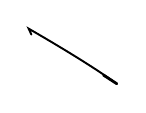
\begin{tikzpicture}[x=1cm,y=1cm,line cap=round]
\draw[line width=0.7pt] (0.035,-0.075) -- (0,0) .. controls (0.33,-0.19) and (0.80,-0.47) .. (1.12,-0.70);
\draw[line width=1.0pt] (0.95,-0.59) -- (1.12,-0.70);
\end{tikzpicture}}
\margin{117}

\scanpage{119}
\mspage{58}

14. Digression cohomologique (sur \unsure{les|le} ``bouchage des
trous).

Soit $X$ un schéma loc. noeth. \uline{régulier} de
\unsure{dim.} $1$, $S$ un sous-schéma fermé \inserted{réduit discret} tel que
$\forall s\in S$, $\dim_s S=1$ (donc $S$ défini par une
partie fermée discrète de $X$), $U=X\setminus S$.
\margin{Il vaudrait peut-être mieux démarrer avec \unsure{le cas purement topologique|les cas purement topologiques} d'une surface\dots{} et faire le lien avec les groupes \uline{discrets}.}

On veut expliciter par voie galoisienne les
faisceaux \inserted{d'ens.} étales \inserted{constructibles} sur $X$ tels que $F\mid U$ soit
loc. ct. Par le \unsure{topos|tapis} d'Artin \inserted{sur les ouverts du topos}, ils corres-
pondent aux triples
\[
(F_U,F_S,\varphi)
\]
où $F_U$ est un faisceau \inserted{constr.} loc. constant sur $U$,
$F_S$ un faisceau (\unsure{néc.|nécess.} loc. constant)
et $\varphi$ un hom
\[
F_S\xrightarrow{\varphi}j^{*}i_{*}(F_U)
\]
(où $i:U\unsure{\hookrightarrow|\to}X$ et $j:S\to X$ sont les inclusions).
Toute condition de constructibilité étant mise à
part, un faisceau étale $F$ sur $X$ correspond
à un tel triple --- on se restreint ici aux
$F$ tels que $F_U$ \deleted{\unsure{provienne}} provienne du
topos fondamental $B_{\unsure{\Pi_1(U)|\pi_1(U)}}$ de $U$ \deleted{\illegible{1}}\dots
(Il n'y a pas lieu de supposer $F_U$ à fibres finies,

\margin{118}

\scanpage{120}

pour ce qui suit). \deleted{Nous allons}

Soit $\forall s\in S$ $\underline{O}_s$ un hensélisé de $\underline{O}_{X,s}$,
$D_s=\operatorname{Spec}\underline{O}_s$ \inserted{(``disque en $s$'')}, $D_s^{*}=D_s-\{s\}$ \inserted{$=\operatorname{Spec}K_s$ ($K_s$ corps des fractions de $\underline{O}_s$)} (``disque pointé'' en
$s$) $D=\coprod_{s\in S}D_s$, $\unsure{D_s^{*}|D^{*}}=\coprod_{s\in S}D_s^{*}$. On a
un diagramme commutatif
\diagram{\begin{tikzcd}[ampersand replacement=\&]
\& D^{*} \arrow[dl, "\rho"'] \arrow[dr, "\sigma"] \& \& \\
U \arrow[dr, "i"'] \& \& D \arrow[dl, "\unsure{k|\kappa}"] \& S \arrow[l, dashed, "j_0"'] \arrow[dll, dashed, "j"] \\
\& X \& \&
\end{tikzcd}
[La branche pointillée $S\xrightarrow{j_0}D$ est placée entre parenthèses.]}
et on voit \inserted{(par Artin)} que ce diagramme \deleted{\unsure{fait de}} \inserted{permet d'exprimer}
\inserted{les faisceaux} \deleted{topos} étales de $X$ \deleted{\unsure{comme amalgamé}}
\deleted{des topos étales de $U,D$ sur $D^{*}$}
\deleted{\diagram{\begin{tikzcd}[ampersand replacement=\&,column sep=2.5em,row sep=2em]
\& \deleted{\unsure{D^*_{\mathrm{\acute et}}}} \arrow[dl] \arrow[dr] \& \\
\deleted{U_{\mathrm{\acute et}}} \& \& \deleted{D_{\mathrm{\acute et}}}
\end{tikzcd}}}
comme des systèmes \deleted{de faisceaux} \inserted{$(F_U,F_D,\varphi)$}
avec $F_U$ faisceau étale sur $U$, $F_D$ faisceau
étale ``ess\textsuperscript{t} loc. constant'' sur $D$ [NB l'
inclusion $S\to D$ définit une équivalence
entre la cat. de ces faisceaux sur $D$, et
celle des faisceaux étales sur $S$] et
un hom. de faisceaux $F_D\to\sigma_{*}\rho^{*}F_U$ ou encore

\margin{119}
\scanpage{121}
\mspage{59}
% L01
\[
\boxed{\sigma^{*}(F_D)\xrightarrow{\varphi}\rho^{*}(F_U)}
\]
% L02
Or, \deleted{\unsure{cette donnée si $F_U$ est un}} \inserted{si on se borne aux} $F_U$ tels que $F_U$ soit
% L03
lui-= ess$^{t}$. loc$^{t}$ constant, alors les données
% L04
$F_U,F_D,\varphi$ ne font intervenir que des
% L05
faisceaux ess$^{t}$ loc. constants, i.e. des
% L06
topos fondamentaux (multigaloisiens)
% L07
associés aux schémas envisagés, \deleted{\unsure{savoir}} donc
% L08
se décrivent entièrement en termes des
% L09
diagrammes
\diagram{\begin{tikzcd}[ampersand replacement=\&]
 \& B_{\pi_1,D^{*}} \arrow[dl,"{\deleted{\illegible{1}}\,\rho}"'] \arrow[dr,no head,"\sigma"] \& \\
 B_{\pi_1,U} \& \& B_{\pi_1,D}
\end{tikzcd}}
\margin{(*)}
% L10
-- d'ailleurs le cas où $\varphi$ est un \uline{iso} correspond
% L11
justement au cas des faisceaux loc. ess.
% L12
constants sur $X$, i.e. de faisceaux sur
% L13
$B_{\pi_1,X}$ -- lequel topos fondamental
% L14
apparaît donc comme somme
% L15
amalgamée du diagramme de topos
% L16
précédent, s'insérant dans le carré
\diagram{\begin{tikzcd}[ampersand replacement=\&]
 \& B_{\pi_1,D^{*}} \arrow[dl] \arrow[dr] \& \\
 B_{\pi_1,U} \arrow[dr] \& \& B_{\pi_1,D} \arrow[dl] \\
 \& B_{\pi_1,X} \&
\end{tikzcd}}

\scanpage{122}
% L01
Supposons pour simplifier $U$ connexe,
% L02
choisissons un rev. universel \inserted{$\widetilde U$} de $U$, et un
% L03
rev. universel \inserted{$\widetilde D_i^{*}$} de chaque $D_i^{*}$ -- d'où un
% L04
rev. universel \inserted{$\widetilde D_i$} de $D_i$ -- et des isom.
% L05
(= ``classes de chemins'') entre $\rho_{!}(\widetilde D_i^{*})$ et $\widetilde U$
% L06
-- donc le diagramme des topos \unsure{(*)},
% L07
-- ou des groupoïdes fondamentaux --
% L08
s'explicite en termes d'un diagramme
% L09
\diagram{\begin{tikzcd}[ampersand replacement=\&,column sep=large]
 \& {\begin{gathered}
 (\operatorname{Gal}(\overline K_i/K_i))\\[-2pt]
 \Vert\\[-2pt]
 \mathcal E_i
 \end{gathered}} \arrow[dl,"\unsure{\rho_i|\varphi_i}"'] \arrow[dr,"\sigma_i"] \& \\
 {\begin{gathered}
 \mathcal E\\[-2pt]
 \Vert\\[-2pt]
 (\pi_1(U,\widetilde U)=\operatorname{Aut}_U(\widetilde U))
 \end{gathered}} \& \&
 {\begin{gathered}
 \Gamma_i\;\illegible{1}\\[-2pt]
 \Vert\\[-2pt]
 (\operatorname{Gal}(\overline{k(s)}/k(s)))
 \end{gathered}}
\end{tikzcd}}
% L10
et la donnée d'un $F$ comme envisagé sur
% L11
$X$ revient à la donnée d'un système
% L12
$(E_U,(E_i)_{i\in I},(\varphi_i)_{i\in I})$, où $E_U$ est un $\mathcal E$-ens,
% L13
$E_i$ un $\Gamma_i$-ens, $(\forall i\in I)$, et $\varphi_i$ un
% L14
$\mathcal E_i$-hom de $E_i$ dans $E_U$ (i.e. un
% L15
un $\Gamma_i$-hom
\[
\varphi_i:\ E_i\longrightarrow E_U^{\Pi_i},
\]

\scanpage{123}
\mspage{60}
% L01
où \deleted{\unsure{$\Pi_i$ est}} $\Pi_i=\unsure{\operatorname{Ker}(\sigma_i)}$ s'insère dans la suite exacte
% L02
\[
1\longrightarrow\Pi_i\longrightarrow\mathcal E_i\longrightarrow\Gamma_i\longrightarrow1
\]

% L03
Le cas où les $E_i\longrightarrow E_U$ sont des iso,
% L04
i.e. les $E_i$ \unsure{s'identifient|s'identifiant} \deleted{\illegible{1}} tous à $E_U$,
% L05
avec action triviale \unsure{de|des} $\Pi_i$ sur $E_U$, correspond
% L06
au cas où $F$ est ess. loc. \unsure{ct|cst} sur $X$,
% L07
d'où aussitôt
% L08
\[
\pi_1(X)=\mathcal E=\pi_1(U)\ \big/\
\substack{\text{ss-groupe \unsure{invariant} engendré}\\
\text{par les }\rho_i(\Pi_i)}.
\]

% L09
Notre propos est celui d'un calcul galoisien
% L10
(si possible) de la cohomologie de $X$ pour
% L11
les $F$ envisagés.
% L12
Soit $B_{X,U}$ le topos \inserted{dont les faisceaux sont} des triples
% L13
$(F_U,F_D,\varphi)$ comme dessus, qui s'envoie
% L14
donc dans le topos $B_{\pi_1,X}$, correspondant
% L15
aux couples pour lesquels $\varphi$ est iso,
% L16
et reçoit le topos $X_{\mathrm{ét}}$ :

\scanpage{124}
% L01
\diagram{\begin{tikzcd}[ampersand replacement=\&]
X_{\mathrm{ét}} \arrow[r,"f"] \& B_{X,U} \arrow[r,"g"] \& B_{\pi_1,X}
\end{tikzcd}}
% L02
On se pose la question

% L03
a) Calcul ``explicite'', en termes de cohomologie
% L04
des groupes profinis, de la cohomologie
% L05
dans le topos abracadabra $B_{X,U}$. (NB.
% L06
\deleted{\unsure{b) le calcul de}} la cohomologie \deleted{\illegible{1}} de
% L07
$B_{\pi_1,X}$ n'est autre que la cohomologie
% L08
galoisienne profinie de $\pi_1(X)=\mathcal E/\ldots$
% L09
calculé plus haut\ldots).

% L10
b) Vérifier si pour un faisceau de
% L11
torsion $F$ sur $B_{X,U}$ l'hom. can.
% L12
\[
H^{*}(B_{X,U},F)\longrightarrow
H^{*}(X_{\mathrm{ét}},f^{*}F)
\]
% L13
est un iso.

% L14
NB Jusqu'à maintenant, l'hyp.
% L15
$\dim X=1$ n'a pas servi, ni l'hyp. noethérien
% L16
-- seulement le fait que $S$ soit partie fermée
% L17
discrète, $X$ connexe\ldots. Pour les calculs qui

\scanpage{125}
\mspage{61}
% L01
suivent, correspondants du \deleted{\illegible{1}} cas où les
% L02
$\unsure{D_s|O_s}$ sont des \unsure{jauges} à corps résiduel $k(s)$
% L03
de car. $0$, on va supposer que
% L04
\[
\Pi_i\simeq\widehat{\mathbb Z}\qquad\text{(non canoniquement)}
\]
% L05
-- en fait, par la théorie Kummérienne on
% L06
a un système de systèmes locaux de Tate
% L07
$\unsure{T_{\mathcal E}}$ \inserted{(sur $\mathcal E$)}, $T_i$ \inserted{(sur $\Gamma_i$)}, et des \inserted{$\mathcal E_i$-}isom. $T_{\mathcal E}\simeq T_i$, \deleted{et \illegible{1}}
% L08
(i.e. un $T_X$ sur lequel opère $\unsure{\widetilde{\mathcal E}|\overline{\mathcal E}}=\mathcal E/\ldots$)
% L09
et on aura un iso. can. Kummérien
% L10
\[
T_i\xrightarrow[\sim]{\unsure{\kappa_i|k_i}}\Pi_i.
\]

% L11
On aimerait pouvoir paraphraser,
% L12
sur $B_{X,U}$, la suite exacte de cohomologie
% L13
bien connue
% L14
\[
\longrightarrow H^i(X,F)\longrightarrow H^i(U,F)
\longrightarrow H^{i+1}_S(X,F)\longrightarrow\cdots
\]
% L15
relative à l'ouvert $U$ du topos $X$, et son
% L16
``complémentaire'' fermé $S$. Or, \deleted{\illegible{2}} \inserted{tout comme}
% L17
$X$ s'insère dans un diagramme de topos
% L18
\diagram{\begin{tikzcd}[ampersand replacement=\&]
 \& D^{*}_{\mathrm{ét}} \arrow[dl] \arrow[dr] \& \& \\
 U_{\mathrm{ét}} \arrow[dr,no head] \& \& D_{\mathrm{ét}} \arrow[dl] \& S_{\mathrm{ét}} \arrow[l,"\unsure{\xi}"'] \\
 \& X_{\mathrm{ét}} \& \&
\end{tikzcd}},

\scanpage{126}
% L01
de = $B_{X,U}$ s'insère dans
% L02
\diagram{\begin{tikzcd}[ampersand replacement=\&]
 \& B_{\pi_1,D^{*}} \arrow[dl] \arrow[dr] \& \& \\
 B_{\pi_1,U} \arrow[dr] \& \& B_{\pi_1,D} \arrow[dl] \& B_{\pi_1,S} \arrow[l,"\approx","\unsure{\xi_{\mathrm{ét}}}"'] \\
 \& B_{X,U} \& \&
\end{tikzcd}}

% L03
[\uline{NB} les $\varprojlim$ finies et $\varinjlim$ quelc.
% L04
dans $B_{X,U}$ i.e. pour les $(F_U,F_D,\varphi)$, se
% L05
calculent ``terme à terme''] Je dis
% L06
que $B_{\pi_1,U}\longrightarrow B_{X,U}$ s'identifie à un
% L07
morphisme d'induction, relatif à l'
% L08
objet \deleted{\illegible{1}} \unsure{(noté encore} $U$ par abus de notation)
% L09
de $B_{X,U}$ défini par
% L10
$F_U={}$faisceau final $e_U$, $F_D={}$faisceau initial $\varnothing_D$
% L11
(et $\varphi$ \unsure{est|étant} alors fixé !). En effet, les
% L12
objets \inserted{de $B_{X,U}$} au dessus de $U$ s'identifient aux
% L13
$(F_U,F_D,\varphi)$ avec $F_D=\varnothing_D$ (ce que fixe $\varphi$ !) donc
% L14
ils forment une cat. équivalente à celle des
% L15
$F_U$, i.e. à $B_{\pi_1,U}$. On voit que le topos
% L16
résiduel (s'identifiant \deleted{aux} \inserted{à la cat. des} $F\deleted{_{\unsure{U}},\unsure{E|e}_{\unsure{i}}}=(F_U,F_D,\varphi)$ tels

\scanpage{127}
\mspage{62}
% L01
que $F_U=e_U$ faisceau final, s'identifie de = à la
% L02
catégorie \inserted{$B_{\pi_1,D}$} des $F_D$ \deleted{\illegible{2}} -- le foncteur
% L03
canonique ``image inverse sur $B_{\pi_1,D}$ de l'image
% L04
directe de $F$ sur $B_{\pi_1,U}$'' n'étant autre
% L05
$\sigma_*\rho^*$, de sorte qu'on retrouve la description
% L06
\deleted{\illegible{1}} typique d'Artin d'un topos déduit
% L07
par ``recollement'' d'un \deleted{\unsure{objet}} ouvert et du
% L08
fermé complémentaire.
% L09
On trouve donc une suite exacte
% L10
\[
\longrightarrow H^i(B_{X,U},F)\longrightarrow
H^i(B_{\pi_1,U},F_U)\longrightarrow
H^{i+1}_{S(\text{ou }D)}(B_{X,U},F)\longrightarrow\cdots
\]
% L11
s'envoyant dans la suite exacte analogue
% L12
relative à $X_{\mathrm{ét}},U_{\mathrm{ét}},S_{\mathrm{ét}}$. \deleted{\unsure{Pour} \illegible{2}} \inserted{(On n'a}
% L13
tjrs pas utilisé d'hyp. spéciale sur $S$\ldots).

% L14
Pour vérifier que l'on a des iso
% L15
au niveau des $H^i(B_{X,U},F)\longrightarrow H^i(X_{\mathrm{ét}},F)$,
% L16
il suffit par le lemme des cinq de
% L17
le prouver au niveau des
% L18
$H^i(B_{\pi_1,U},F)\longrightarrow H^i(U_{\mathrm{ét}},F)$ [i.e. \unsure{vérifier|vérifions} que la
% L19
cohomologie de $U_{\mathrm{ét}}$ ``se calcule galoisiennement'']
% L20
\uline{et} au niveau des $H^i_S$. \deleted{\unsure{Or}} Regardons,

\scanpage{128}
% L01
d'abord ces derniers -- on a
% L02
$H^0_S(B_{X,U},E)={}$ ens des sections de $F$ [i.e. des
% L03
couples d'une section de $F_U$ et
% L04
d'une de $F_D$, se correspondant
% L05
par $\varphi$, i.e. d'un élément \inserted{$x$} de
% L06
$E_U$ invariant par $\mathcal E$, et des
% L07
$x_i\in E_i$ invariants par les $\Gamma_i$,
% L08
tels que $x=\varphi_i(x_i)\quad\forall i$]
% L09
tels que $x=0$ \deleted{\unsure{des|dans} \unsure{systèmes}}
% L10
\[
=\prod_i(\operatorname{Ker}(E_i\longrightarrow E_U)
\]
% L11
on constate que ce foncteur se factorise
% L12
par le foncteur $H^0_S$ relatif à ``l'inclusion''
% L13
\deleted{\unsure{$D^{*}\subset D$} \unsure{ou} $B_{\pi_1,D^{*}}\longrightarrow B_{\pi_1,D}$}
% L14
analogue \deleted{\illegible{1} $B_{\pi_1,U}$ \illegible{2}}
% L15
\[
B_{\underbrace{\pi_1,\unsure{D^{*}|D_{*}}}_{\text{remplaçant }\pi_1,U}}\longrightarrow B_{D,D^{*}}\quad\ldots
\]
% L16
et les $H^i_S$ sur $D_{X,U}$ se calculent comme
% L17
\deleted{\unsure{qui n'est autre que}}
% L18
ceux dans la situation locale $B_{D\deleted{\illegible{1}},D^{*}\deleted{\illegible{1}}}$ --
% L19
où on trouve le calcul habituel en
% L20
termes de l'hom. de groupes $\mathcal E_i\longrightarrow\Gamma_i$.
\margin{que j'ai un peu oublié !}

% L21
Mais dans le cas actuel, l'hyp. $\dim_s X=1$
% L22
aux pts de $s\in S$, \deleted{et $X$ \unsure{rég.}} implique que
% L23
la situation \inserted{de topos} localisée $D^{*}_{\unsure{a|\mathrm{ét}}}\hookrightarrow D_{\unsure{a|\mathrm{ét}}}$ est déjà entièrement
% L24
définie en termes des topos fondamentaux \unsure{des}

\scanpage{129}
\mspage{63}
% L01
\deleted{\unsure{des termes de}}
% L02
i.e. le topos $B_{D,D^{*}}$ est équivalent à
% L03
$D_{\mathrm{ét}}$ -- or les $H^i_S(X_{\mathrm{ét}},F)$ se calculent
% L04
bien sur $D_{\mathrm{ét}}$\ldots On trouve donc

% L05
\uline{Prop.} L'hom. de suites exactes de coho-
% L06
mologie envisagé est un isomorphisme,
% L07
pourvu que l'on sache que l'hom.
% L08
$H^i(\mathcal E,F_{\mathcal E})\xrightarrow{\sim}H^i(U_{\mathrm{ét}},F_U)$ est un isom.
% L09
pour $\forall i$ ($F_U$ faisceau \unsure{étale|ét. loc.} sur $U_{\mathrm{ét}}$
% L10
défini par un groupe $F_{\mathcal E}$ sur lequel $\mathcal E=\pi_1(U)$
% L11
opère).

% L12
\uline{Exemple} : \inserted{OK} Si $U$ est une courbe affine
% L13
sur $k$ alg. clos \inserted{$F$ \deleted{\illegible{1}} premier à car} (car OK pour $i=0,1$, et
% L14
pour $i=2$, les deux \unsure{mbres} sont nuls
% L15
(la \unsure{ch.|coh.} galoisienne, car le groupe fondamental
% L16
\inserted{premier à $p$} est \deleted{pro} libre\ldots) -- d'où on déduit le
% L17
cas analogue pour $\unsure{U|X}$ affine sur $k$ quelcon-
% L18
que, puis = si $U$ n'est pas affine mais
% L19
simplement quasi-projective ? \deleted{\illegible{1}}
\margin{\uline{Cor.} Dans ce cas, la cohomologie de $X$ à coefficients dans un $F_X$ loc. const. \unsure{se} calcule également galoisiennement ? Non, à cause du genre $0$ !!! Dans le cas des courbes projectives lisses de genre $\ne0$ il faut un argument spécial.}

% L20
Nous nous intéressons maintenant au
% L21
cas où $X$ projective \inserted{(connexe)} sur $k$ alg. clos, \unsure{on voit donc|on sait donc}

\scanpage{130}
% L01
que : \deleted{les $H^i_!(U,F$}
% L02
a) Si $S=\varnothing$ i.e. $X=U$, la cohomologie de $U$
% L03
à (coefficients dans les syst. locaux) est celle
% L04
de $\pi$. Donc\ldots un isom. can.
% L05
\[
H^2(\pi,T)\simeq H^2(X,T)\quad(\simeq\widehat{\mathbb Z})
\]
\margin{avec \unsure{grain|grains} de sel en car. $p>0$}
% L06
\deleted{b) Si $S=$}

% L07
b) Si $S\ne\varnothing$, les $H^i_!(U,-)$ se \unsure{déterminent|décrivent}
% L08
et calculent par voie galoisienne, en termes
% L09
des \deleted{\unsure{syst.}} \inserted{groupes} à lacets, permettant de reconsti-
% L10
tuer la situation
% L11
\diagram{\begin{tikzcd}[ampersand replacement=\&,column sep=large]
 \& B_{\pi_1,D^{*}} \arrow[dl] \arrow[dr] \& \\
 B_{\pi_1,U} \arrow[dr,dotted,no head] \& \&
 {\begin{gathered}
 B_{\pi_1,D}\ (={\text{topos discret défini}}\\
 {\text{par }}S=I)
 \end{gathered}} \arrow[dl,dashed] \\
 \& B_{U,X} \&
\end{tikzcd}}
% L12
en postulant que le composant $B_{\pi_1,D_i^{*}}$
% L13
n'est autre que $B_{L_i}$ (avec les
% L14
\unsure{notations} du \unsure{n$^{o}$|cas} précédent). On
% L15
trouve alors des iso can. (par calculs locaux)
% L16
\[
H^2_{\unsure{S_i|s_i}}(B_{U,X},\unsure{L_i})\simeq\widehat{\mathbb Z}
\quad\text{i.e.}\quad
H^2_{\unsure{S_i|s_i}}(B_{U,X},\widehat{\mathbb Z})\simeq L_i^{\otimes-1}
\]
% L17
(si $g\ne0$)
\[
H^2_{\unsure{S_i|s_i}}(B_{U,X},\widehat{\mathbb Z})
\xrightarrow{\sim}H^2(X,\widehat{\mathbb Z})
\simeq H^2(\pi,\widehat{\mathbb Z})
\]
% L18
d'où \unsure{en} \deleted{\unsure{résumé}} mettant ensemble, des iso
% L19
canoniques
\[
\deleted{\unsure{H}}\quad L_i\simeq H^2(\pi,\widehat{\mathbb Z})^{\otimes-1}.
\]
\margin{Mais dans tous les cas (= si $g=0$, du moment \unsure{qu'on} n'a pas $\nu=0$) \deleted{\illegible{1}} on trouve $H^{2}_{!}(B_{\pi_1,U},\widehat{\mathbb Z})\simeq\unsure{\widehat T_{\pi}^{\otimes-1}|T_{\pi}^{\otimes-1}}$ canoniquement, d'où une description \unsure{cohom.} des \unsure{modules d'orientations}, commune au \unsure{cas sans trous et avec} trous\ldots}
\scanpage{131}
\mspage{64}

On constate que les composés
\[
T_\pi \xrightarrow{\sim} L_i \longrightarrow
H^2(\pi,\widehat{\mathbb Z})^{\otimes-1}
\]
ne dépendent pas du choix de $i$, de sorte que le module d'orientation $T_\pi$ du groupe \inserted{profini $\pi$} à lacets $\pi$ s'identifie au \uline{dual} de $H^2(\pi,\widehat{\mathbb Z})$ (si $g\ne0$).

Considérons maintenant un hom. de groupes à lacets
\[
\begin{gathered}
\pi'\xrightarrow{f}\pi\\
I'_0\xrightarrow{\tau}I
\end{gathered}
\]
associé à un isom $T_{\pi'}\simeq T_\pi$ et une application degré
$d:I'_0\longrightarrow\mathbb N$
\deleted{(\unsure{entiers} \illegible{3}}
(NB $i'\in I'\setminus I'_0\longrightarrow f(L'_{i'})=(1)$.

On voudrait en déduire un diagramme de morphismes de topos
\diagram{\begin{tikzcd}[ampersand replacement=\&]
B_{\Pi_1 U'} \arrow[r,dash] \arrow[d] \& B_{\deleted{\unsure{\Pi_1}}X',U'} \arrow[r,dash] \arrow[d] \& B_{\Pi_1 X'} \arrow[d] \\
B_{\Pi_1 U} \arrow[r,dash] \& B_{\deleted{\unsure{\Pi_1}}X,U} \arrow[r,dash] \& B_{\Pi_1 X}
\end{tikzcd}}
et un hom \uline{trace} sur la cohomologie à supports propres de $U',U$ (défini en termes de cohomologie sur $B_{X',U'}, B_{X,U}$ relativement)
\deleted{\unsure{qui un iso}} \unsure{induisant} \deleted{\unsure{pour}} un \uline{iso}
\[
H^2_!(U',\widehat{\mathbb Z})\longrightarrow
H^2_!(U,\widehat{\mathbb Z})
\]

\scanpage{132}

qui soit justement \inserted{(\unsure{contragrédient|contragrédiant} de)} (l'isom des modules d'orientation associé à $f$....

14. Où on revient sur les morphismes \uline{mixtes} (correspondants, dans le cadre topologique, au cas de
$f:(X',S')\longrightarrow(X,S)$ tels que l'on ait
$[f(X'\setminus S')\subset X\setminus S$, i.e.\ \inserted{$S'\supset f^{-1}(S)$,} \inserted{mais}$]$
\deleted{\illegible{1}} ($S'\ne f^{-1}(S)$, i.e.\ il y a des pts de $\unsure{S'|S}$ qui sont envoyés dans $U=X\setminus S$.
\margin{$X,X'$ $T$-orientés}

Dans le \deleted{langage} \inserted{paradigme} topossique et groupoïdal, $(X,S)$ est \deleted{défini} \inserted{décrit} par un diagramme de groupoïdes
\[
\Pi_{D^*}\longrightarrow\Pi_U
\qquad
(\text{et }k:T_{\Pi_{D^*}}\simeq
\text{ système local des }\pi_1\text{ sur }\Pi_{D^*})
\]
\deleted{\illegible{1}}
ou de topos
\[
B_{D^*}\longrightarrow B_U
\]
et \deleted{\unsure{un}} isom \inserted{$k$} du syst. local des $\pi_1$ sur $B_{D^*}$, dans le système \inserted{loc.} constant $T$,
\deleted{\illegible{4} $(\deleted{\unsure{X}},U')$}
\inserted{qui permet de définir $B_D\;(=B_{\unsure{\pi_0 D_*}})$ (le topos discret)}
et le topos $B_{X,U}$, s'insérant dans le diagramme \deleted{$\unsure{B_{\Pi_1 D^*}}$} de topos

\scanpage{133}
\mspage{65}

\diagram{\begin{tikzcd}[ampersand replacement=\&,column sep=large]
\& B_{D^*}\arrow[dl,"\rho"']\arrow[dr,"\sigma"] \& \\
B_U\arrow[dr,"\varphi"'] \&\& B_D\; (\text{topos discret }\xleftarrow{\sim} B_S)\arrow[dl,"\psi"] \\
\& B_{X,U} \&
\end{tikzcd}}
où $\varphi,\psi$ sont des morphismes d'\unsure{inclusion|induction} de sous-topos, $\varphi$ ouvert $\psi$ fermé, complémentaires l'un de l'autre, et itou pour $(X',S')$, décrit par un diagramme analogue
\diagram{\begin{tikzcd}[ampersand replacement=\&]
\& B_{D'^*}\arrow[dl]\arrow[dr] \& \\
B_{U'}\arrow[dr] \&\& B_{D'}\simeq\unsure{B_{S'}|B_S}\arrow[dl] \\
\& B_{X',U'} \&
\end{tikzcd}}

Ceci dit, on veut absolument, dans une description de
$f:(X',S')\longrightarrow(X,S)$, que celle-ci permette de retrouver non seulement $B_{U'}\longrightarrow B_U$ (ce qui sera acquis par la donnée d'un $f_\pi:\pi'\longrightarrow\pi$), mais aussi
\[
B_{X',U'}\longrightarrow B_{X,U}\qquad\unsure{g|q}.
\]
On aura \deleted{\unsure{$S$}}
\[
S'=\underset{\substack{\Vert\\f^{-1}(S)}}{S'_0}\amalg S'_1,
\quad\text{donc}\quad D'=D'_0\amalg D'_1,
\]

\scanpage{134}
\mspage{66}

et en fait $f$ induit $S'_1\xrightarrow{f}U$ (et non $S'_1\longrightarrow S$) qui doit s'expliciter, au niveau \deleted{\illegible{2}} des topos multigaloisiens, par un morphisme
\diagram{\begin{tikzcd}[ampersand replacement=\&]
B_{D'_1}\arrow[r] \& B_U \\
B_{S'_1}\arrow[u,"\simeq",draw=none] \&
\end{tikzcd}}
i.e.\ par la donnée d'une famille de rev. universels de $U$, paramétrée par $S'_1=I'_1$, ou (\unsure{si un tel} rev. universel est choisi, $U$ étant connexe, d'où un $\pi=\operatorname{Aut}(\widetilde U)$) par une famille de torseurs sous \deleted{\unsure{le}} $\pi$, $(P_{i'})_{i'\in I'_1}$.
Ceci étant \deleted{\unsure{défini}} \inserted{posé} on \unsure{pourra} décrire, en termes de
\diagram{\begin{tikzcd}[ampersand replacement=\&,column sep=3.5em,row sep=3em]
B_{D_0'{}^*} \arrow[r,no head] \arrow[d] \& B_{U'} \arrow[d] \\
B_{D^*} \arrow[r,no head]
\arrow[ur,bend left=30,shorten <=1.5em,shorten >=1.5em,"\sim"'] \& B_U
\end{tikzcd}}
et de
\[
B_{D_1'^*}\longrightarrow B_{D'_1}\longrightarrow B_U
\]
\deleted{\unsure{un}} l'hom de topos $B_{X',U'}\longrightarrow B_{X,U}$
% a small double tick stands before $B_{X',U'}$ (below $B_{D'_1}$ of the display above): probably the call of the marginal note
--- je passe sur le détail de la description
\margin{Il semble qu'on soit en droit de faire la description des morphismes de topos $B_{X',U'}\longrightarrow B_{X,U}$ qui induisent $U'\longrightarrow U$ et qui sur $D_1'^*$ \unsure{$(=D'^*\vert U$} \deleted{\illegible{2}}, se factorisent par $D_1'^*\longrightarrow D'_1$...}

\scanpage{135}

Quand on se donne un groupe d'opérateurs \deleted{$\Sigma$}$\Gamma$ sur la situation $(X',S')\longrightarrow(X,S)$ donc sur la situation groupoïdale ou topossique, il faut en tenir compte dans la description ci-dessus.
Ainsi $I'_0$ et $I'_1$ sont stables par $\Gamma$, et le morphisme \deleted{\illegible{1}} $B_{\unsure{D'_1}}\longrightarrow B_U$ doit être stable par $\Gamma$.
\deleted{On a donc un \unsure{joli} ensemble $\unsure{E_f=\bigcup E_i}$ ---}
\deleted{En termes d'un rev. universel $\widetilde U$ de $U$, considérons les \deleted{\illegible{1}} ens $\unsure{\operatorname{Hom}}(f_*(\unsure{s'_{i'}}),\widetilde U)$}
Ce qui signifie aussi, sans doute, qu'on a un morphisme de topos de
$B_{D'_1,\Sigma}=B_{I'_1,\unsure{\Sigma|\Gamma}}$
dans $B_{U,\deleted{\Sigma}\Gamma}$.
Choisissant pour tte orbite de $\Gamma$ dans $I'_1$ un représentant $s'\in I'_1$, et considérant son stabilisateur $\Gamma_{s'}\subset\Gamma$, il faut donc pour tte telle orbite i.e.\ \deleted{\unsure{tte}} tt $i'$ se donner un $\Gamma_{s'}$ objet de la cat. des rev. universels de $(U,\Gamma)$.
\unsure{Simultanément|Équivalemment} \deleted{donc} Décrivant $(U,\Gamma)$ en termes

\scanpage{136}
\mspage{67}

d'une extension $\mathcal E$ de $\Sigma\subset\Gamma$ par $\pi$ (en choisissant un rev. universel $\widetilde U$ de $U$), la donnée de $B_{\Gamma_{s'}}\longrightarrow B_{X,U}$ compatible avec tout revient sauf erreur à la donnée d'un torseur $P$ à droite sous $\pi$ (permettant de tordre le revêtement universel \unsure{de référence} $\widetilde U$ de $\unsure{U^\Gamma|U,}$ à l'aide de $P$ \deleted{et} \inserted{donc aussi de tordre $\mathcal E$ par $P$}), et d'un scindage de $\mathcal E^P\longrightarrow\Gamma$ au dessus de $\Gamma_{s'}$.
[La classe d'isomorphie d'un tel objet $\longrightarrow$ une classe de $\pi$-conjugaison de scindages de $\mathcal E\longrightarrow\Gamma$ au dessus de $\Gamma_{s'}$... ).

Un autom d'un tel couple \deleted{correspond} $P,\ \Gamma_{s'}\xrightarrow{q}\mathcal E^P$ correspond à un $\alpha\in\pi$ qui \uline{centralise} $\Gamma_{s'}$, \inserted{i.e.\ qui soit fixé par $\Gamma_{s'}$ opérant sur $\pi$.} (Si les $\Gamma_{s'}$ opèrent assez fortement sur $\pi$ pour que l'on sache que $\pi^{\Gamma_{s'}}=(1)$, l'objet $(P,q:\Gamma_{s'}\longrightarrow\mathcal E^P)$ est défini à \uline{isom unique} près par la classe d'isomorphie \deleted{\unsure{de celui-ci}} (classe de scindages de $\mathcal E$ sur $\Gamma_{s'}$).
\margin{\unsure{!!!|[trois traits verticaux]}}
Il me semble probable que ceci soit tjrs le cas dans le cas \uline{arithmétique}, où $\Gamma_{s'}$ est un ss-groupe ouvert du groupe de Galois $\Gamma_{\unsure{k|K}}$ (dont l'opération extérieure est \inserted{draconienne !}).

\scanpage{137}

Ceci va en direction de la conjecture qu'une classe de scindage de $\mathcal E$ sur $\Gamma$ est ``aussi bonne'' qu'un pt rat. de $U$ sur $K$ --- et permet de paradigmer ce qu'un tel pt rationnel permettrait d'obtenir....

\textcircled{15} \uline{Retour sur le cas topologique} Soit $\Gamma$ un grpe fini opérant sur un grpe à lacets $\pi$ --- supposons que ceci provienne d'une situation topologique, $\Gamma$ opérant sur $(X,S)$. Il y a des pts à vérifier (cas \uline{\unsure{anabéliens|anabélien}})
\margin{Structure des $\Gamma$-orbites critiques en termes d'extension...}

\[
\text{a) Opération de }\Gamma\text{ triviale}
\quad\Longleftrightarrow\quad
\underset{\text{triviale}}{\Gamma\longrightarrow\operatorname{Autext}(\pi)}
\]
en d'autres termes : un autom d'ordre fini de $(X,S)$ ne peut être isotope à l'identité (ou $\overline{\mathrm m}$ \inserted{seulement} homotope, cela revient au $\overline{\mathrm m}$ d'ailleurs) que si elle est triviale.

C'est $\overline{\mathrm m}$ connu en Géom. Alg ``abstraite'', du moment qu'on admet que $u$ \unsure{conserve|préserve} une structure \deleted{\unsure{complexe}} \inserted{complexe}, \deleted{\unsure{conforme}} \inserted{\unsure{il en est justement}}

\scanpage{138}
\mspage{68}

ainsi si on \deleted{suppose} \inserted{admet} qu'il n'y a pas de sauvagerie.... Sans doute tte action d'un groupe fini $\Gamma$ laisse structure conforme invariante, \deleted{\illegible{1}} donc sa restriction à
\[
\Gamma^0=\operatorname{Ker}(\Gamma\xrightarrow{\chi}\{\pm1\})
\]
laisse structure complexe invariante.

Supposons dorénavant que $\Gamma$ opère fidèlement, \inserted{$\Gamma\ne1$,} \deleted{\illegible{1}} Le choix d'une structure complexe sur $Y=X/\Gamma^0$ \inserted{en définit une sur $X$;} (NB: \deleted{\illegible{1}} $\Gamma/\Gamma^0$ opère encore \inserted{sur $X/\Gamma^0$} en fait \deleted{$X/\Gamma^0$} \unsure{si} $\Gamma\ne\Gamma^0$ i.e.\ $\Gamma/\Gamma^0\simeq\{\pm1\}$, $X/\Gamma^0$ est munie d'une ``structure de \deleted{\illegible{2}} courbe algébrique \inserted{str. conforme} réelle''... ) stable par $\Gamma^0$ --- et (stable par $\Gamma$ si on choisit celle de $Y$ \deleted{\unsure{invariante}} \inserted{invariée} par \unsure{l'élément|l'élt} non trivial de $\Gamma/\Gamma^0$ (s'il y en a).).
\margin{\unsure{marche|comme} chaque fois qu'on a un rev. ramifié de surfaces conformes}

\deleted{Or} Tout $x\in U^\Gamma$ définit une classe \deleted{\illegible{1}} \inserted{\deleted{\unsure{classe}} de $\pi$-conj. de} scindages de l'extension $\mathcal E$ de $\Gamma$ par $\pi$, comme on voit en prenant $x$ comme pt base. ! Noter que $U^\Gamma$ est un ens fini \inserted{si $\Gamma^0\ne1$, [i.e.\ $\Gamma$ pas réduit à une \deleted{\illegible{1}} \unsure{anti-involution} \illegible{1})}.
\margin{\uline{NB} $U^\Gamma\ne\varnothing$ implique que $\Gamma^0$ est cyclique...}
On trouve \deleted{donc} une application
\[
U^\Gamma\longrightarrow\text{ens des classes de }\pi\text{-conjugaison de scindages de }\mathcal E\longrightarrow\Gamma,
\]

\scanpage{139}
\mspage{69}

i.e.\ \unsure{ens|aux} des relèvements de $\Gamma\longrightarrow\operatorname{Autext}\pi$ \inserted{en} $\Gamma\longrightarrow\operatorname{Aut}(\pi)$, mod $\pi$-conjugaison.

\uline{Question} \inserted{(Si $\Gamma^0\ne(1)$)} Cette application est-elle bijective ??

[Si $\Gamma^0=\{1\}$, $\Gamma/\Gamma^0\simeq\{\pm1\}$, alors $X^\Gamma$ est l'ens des pts réels d'une courbe alg. réelle et $U^\Gamma=X^\Gamma-S^\Gamma$ est le complémentaire d'une partie finie dedans, on a
\[
\pi_0(X^\Gamma-S^\Gamma)\longrightarrow
\pi\text{-classes de scindages de }\mathcal E\text{ sur }\Gamma
\]
et la \deleted{\illegible{1}} question \uline{analogue} de bijectivité se pose, pour ext. de $\pm1$ par $\pi$... ]

Pour l'injectivité de l'application ds le cas $\Gamma^0\ne(1)$, OPS $\Gamma=\unsure{\Gamma^0_a|\Gamma^0}\simeq\mathbb Z/p\mathbb Z$, avec $p$ premier, i.e.\ $\Gamma$ engendré par un autom complexe \inserted{$\unsure{\gamma|y}$} d'ordre $p$, qui définit (si $x,y\in U^\Gamma$, $x\ne y$) un autom d'ordre $p$ de $\pi_1(U,x)$, \deleted{\unsure{soit}} $u_x$, \unsure{soit} \deleted{une} (donc classe de $\pi$-conj d'automs de $\pi$ d'ordre $p$), et un autre $u_y$.
Il faut prouver que $u_x,u_y$ ne sont pas conjugués sous $\pi$

\scanpage{140}

\uline{Théorème} Soient $\unsure{U|X}$ \deleted{\unsure{une surface}} \inserted{espace} topologique connexe \inserted{(\deleted{\illegible{2}}, par arcs)}, $\Gamma$ un groupe fini opérant \deleted{fidèlement} sur $U$, $\widetilde U$ un revêtement universel de $U$, d'où \deleted{opérant} un groupe extension
\[
1\longrightarrow\pi\xrightarrow{i}\mathcal E\xrightarrow{p}\Gamma\longrightarrow1
\]
opérant fidèlement sur $\widetilde U$ ($\pi=\operatorname{Aut}_U(\widetilde U)\simeq\pi_1(U)$... ).
Pour tout point fixe $x\in U^\Gamma$, $\Gamma$ opère sur le revêtement universel \unsure{ponctué|pointé} sur $x$, soit \deleted{\illegible{1}} $\unsure{R_x|\mathcal R_x}$, en laissant fixe le pt \inserted{marqué} $\widetilde x$ de $\unsure{R_x}$ au dessus de $x$, d'où un scindage de l'extension relative à $\unsure{R_x}$
\diagram{\begin{tikzcd}[ampersand replacement=\&]
1\arrow[r] \& \pi_x\arrow[r,"i_x"] \& \mathcal E_x\arrow[r,"p_x"] \& \Gamma\arrow[r]\arrow[l,bend left=40,"\sigma_x"] \& 1
\end{tikzcd}}
et pour tt \deleted{choix de chemin} \inserted{isomorphisme} $\ell$ \inserted{(``chemin'')} $\unsure{R_x}\simeq\widetilde U$, induisant un isomorphisme d'extensions $\mathcal E_x\xrightarrow{\sim}\mathcal E$ (défini \unsure{de|dans} mod comp. avec un autom intérieur induit par un $\alpha\in\pi$... ) on trouve \uline{par transport} de structure un scindage $\sigma_{x,\ell}$ de $\mathcal E\xrightarrow{p}\Gamma$, (qui, pour $\ell$ variable, est défini à autom intérieur près par un $\alpha\in\pi$).
On trouve ainsi une application
\[
(*)\quad U^\Gamma\longrightarrow
\begin{gathered}
\text{classes de }\pi\text{-conj. de scindages}\\
\text{de l'extension }\mathcal E\text{ de }\Gamma\text{ par }\pi\\
=\text{classes de }\pi\text{-conj. de ss-grpes }\inserted{\unsure{sections}}\ \Gamma'\text{ de }\mathcal E
\end{gathered}
\]
\scanpage{141}
\mspage{70}

L'image de cette application est donc formée des \inserted{classes de $\pi$-conj. des} sous-groupes sections $\Gamma'\subset\mathcal E$ tels que $\widetilde U^{\Gamma'}\ne\varnothing$, et pour un tel $\Gamma'$, l'ens. des \unsure{$x\in U^\Gamma$} qui \deleted{\unsure{lui}} donnent comme image cette classe de conj. est l'image de $U^{\Gamma'}$ dans $U$. Enfin, si $x$ est dans cette image, l'ens. \inserted{$\widetilde U^{\Gamma'}_x$} des $\widetilde x\in\widetilde U^{\Gamma'}$ au dessus de $x$ (\deleted{\unsure{$\ne\varnothing$}} hyp. sur \unsure{a|x}) est un torseur sous $\pi^{\Gamma'}$ i.e. si $\widetilde x\in(\widetilde U^{\Gamma'})_x$, \deleted{\unsure{de}} et si $\alpha\in\pi$, alors
\[
\alpha.\widetilde x\in\widetilde U^{\Gamma'}\quad\Longleftrightarrow\quad\alpha\in\pi^{\Gamma'}
\]
(Vérification triviale, comme du reste toutes les assertions précédentes). Ainsi, les conditions suivantes sont équivalentes :

\margin{NB \unsure{$\widetilde U_x$} étant identifié à \unsure{$\operatorname{Isom}_U(R_x,\widetilde U)$}, $\widetilde U_x^{\Gamma'}$ s'identifie à \unsure{$\operatorname{Isom}_{U,\Gamma}(R_x,\widetilde U_{\Gamma'})$} \unsure{des deux isom. qui commutent|des isom. de rev. commutant} à l'action de $\Gamma$ et $\pi^\Gamma=(1)$ signifie que cet isom. est unique \unsure{i.e.} \deleted{\illegible{3}} \unsure{la classe de conj. des sections} \illegible{2}.}

 a) $(*)$ est une bijection, et $\forall$ ss-gpe $\Gamma'$ de $\mathcal E$ section de l'extension, \deleted{\illegible{1}} on a $\pi^{\Gamma'}=\{1\}$.

 b) $\forall\,\Gamma'$ comme dans a), $\Gamma'$ opérant sur $\widetilde U$ a un p\textsuperscript{t} fixe et un seul.

Ceci posé, prouvons le

\uline{Lemme fondamental} Soit $\Gamma$ un groupe \inserted{fini} fini, opérant fidèlement sur \inserted{un espace} \unsure{$D$}\,$\simeq\mathbb R^2$, soit \deleted{On suppose $\Gamma=$} $\Gamma^\circ$ le ss-gpe de $\Gamma$

\mspage{140}

\scanpage{142}

(d'indice $0$ ou $1$) formé des $g\in\Gamma$ tels que $g_D$ conserve l'orientation, et supposons $\Gamma^\circ\ne\{1\}$ (i.e. $\Gamma$ n'est réduit ni au groupe unité, ni au groupe \deleted{\illegible{1}} $\{1,\sigma\}$, où $\sigma$ est une anti-involution de $D$. Alors

 a) $\Gamma$ admet un p\textsuperscript{t} fixe et un seul dans $D$ i.e. $\operatorname{card}D^\Gamma=1$

 b) \deleted{\unsure{Et}} $\Gamma^\circ$ est cyclique, et si $\Gamma\ne\Gamma^\circ$, $\Gamma$ est un groupe \inserted{diédral}.

Plus précisément, il existe un homéomorphisme
\[
D\simeq\mathbb C
\]
tel que \deleted{$\Gamma$ opère par automorphismes} \inserted{\unsure{sur $\mathbb C$ par le groupe}} \deleted{\illegible{1}} d'homéomorphismes de $\mathbb C$ transformé de \deleted{complexes et anti-complexes de $\mathbb C$} \deleted{\unsure{fixant}} $\Gamma$ soit le groupe des homothéties par $\mu_n(\mathbb C)$ (si $\Gamma=\Gamma^\circ$ d'ordre $n$), soit le groupe diédral associé \unsure{$z\longrightarrow\zeta\tau^\varepsilon(z)$} ($\zeta\in\mu_n(\mathbb C)$, $\varepsilon=\pm1$) où \unsure{$\sigma$} \deleted{\illegible{1}} est la conjugaison complexe.

\uline{Démonstration du lemme fondamental.}

\deleted{Supposons d'abord $\Gamma=\Gamma^\circ$, i.e. $\Gamma$ conserve l'orientation. \deleted{Si $\Gamma$ opérait \unsure{sans p\textsuperscript{t}}} On procède}

\mspage{141}

\scanpage{143}
\mspage{71}

\deleted{Par induction sur l'ordre de $\Gamma$.}

\deleted{\unsure{a)} \unsure{$D^\Gamma\ne\varnothing$}}

\deleted{a) Cas $\Gamma$ d'ordre premier}

 a) Supposons d'abord qu'on puisse trouver une structure $C^2$ sur $D$ invariante par $\Gamma$ --- alors un argument standard montre qu'il existe une structure conforme invariante par $\Gamma$, or le th. fondamental de la représentation conforme montre qu'alors
\[
\begin{aligned}
&\text{ou bien }D\simeq\text{intérieur}\ \inserted{\Delta}\ \text{du disque unité }\Delta\ \inserted{\text{ou du demi-pl. de Poincaré}}\\
&\text{ou bien }D\simeq\mathbb C\qquad\text{(isom. conformes).}
\end{aligned}
\]
Dans le premier cas, le groupe des automorphismes \deleted{applications} conformes est
\[
\simeq\unsure{\operatorname{Sl}(2,\mathbb R)^\sim\,|\,\operatorname{Gl}(2,\mathbb R)^\sim}
=\{u\in\operatorname{Gl}(2,\mathbb R)\mid\det u=\pm1\}
\]
(\deleted{opérant par} $u=\left(\begin{smallmatrix}a&b\\c&d\end{smallmatrix}\right)$ opérant sur \deleted{\illegible{1} Poincaré} \inserted{$\widehat{\mathbb C}$} par \deleted{\unsure{$z\longmapsto\dfrac{az+b}{cz+d}$}} $\Theta_u\circ\tau^{\det u}$, où $\tau$ est la conjugaison complexe et $\Theta_u(z)=\dfrac{az+b}{cz+d}$, et laissant stable le demi-pl. de Poincaré), et tt sous-groupe compact est \inserted{contenu dans un} conjugué du \uline{ss-groupe} compact maximal, qui (en repassant au disque unité \inserted{$\Delta$}) s'identifie au groupe $O(2,\mathbb R)$ des

\mspage{142}

\scanpage{144}

transformations du disque unité de la forme
\[
z\longrightarrow\zeta\tau^\varepsilon(z)\qquad
\begin{gathered}
\zeta\in\mathbb U=\{\zeta\in\mathbb C\mid |\zeta|=1\}\\
\varepsilon\in\{\pm1\}\\
\tau\ \text{la conjugaison complexe}
\end{gathered}
\]
Tout ss-groupe fini de ce groupe est de l'un des types explicités plus haut --- on gagne, en utilisant un \unsure{homéom.} $[0,1[\longrightarrow[0,+\infty[$ pour définir un homéom \deleted{\illegible{1}} $\Delta\simeq\mathbb C$ commutant à l'action de $G=\deleted{\unsure{S}}O(2,\mathbb R)$.

Dans le cas $D\simeq\mathbb C$, on voit que \deleted{\unsure{est}} le groupe des autom. conformes de $\mathbb C$ est le groupe des transformations $az+b$ ou $a\overline z+b$, dans lequel un ss-groupe compact maximal est le $\overline{\mathrm m}$ groupe $\deleted{\unsure{S}}O(2,\mathbb R)$ que tantôt --- et tt ss-groupe compact (a fortiori, tt ss-groupe fini) est contenu dans un conjugué de celui-ci. On gagne encore.

Le reste du travail consiste \inserted{ess\textsuperscript{t}} à \deleted{éliminer} montrer que l'hyp. de non sauvagerie

\mspage{143}

\scanpage{145}
\mspage{72}

est toujours satisfaite, \inserted{du moins pour $\Gamma^\circ$. Supposons d'abord $\Gamma=\Gamma^\circ$.} \deleted{On suppose} \inserted{On suppose} que tt est prouvé pour \deleted{les groupes} \inserted{les ordres} $<\operatorname{card}(\Gamma)$. \deleted{Supposons}

 b) $\Gamma$ admet un p\textsuperscript{t} fixe \inserted{\unsure{$o$|$0$}}, i.e. $D^\Gamma\ne\varnothing$.

Sinon, les ss-groupes de stabilité \inserted{$\Gamma_x$} des $x\in D$ étant d'ordre $<$ \deleted{\illegible{1}} $\operatorname{card}\Gamma$, par hyp. de récurrence, les $\Gamma_x$ ont la structure dite dans le th., donc \unsure{$D^\Gamma=U$|$D/\Gamma=U$} est une surface topologique et \unsure{$D\longrightarrow U$|$D\longrightarrow D^\Gamma$} est un rev ramifié, choisissons une structure \deleted{conforme complexe} \inserted{conforme} sur $U$ \deleted{NB $U$ est orienté}; il y a une unique structure conforme sur $D$ telle que $D\longrightarrow U$ soit \deleted{\unsure{conforme|holomorphe}} \inserted{``conforme''} (hol. ou anti-holomorphe), celle-ci est invariante par $\Gamma$, et d'après a) $\Gamma$ admet un p\textsuperscript{t} fixe, contradiction.

 c) $\Gamma$ n'admet pas d'autre p\textsuperscript{t} fixe que \unsure{$o$|$0$}. On fait opérer $\Gamma$ \inserted{\unsure{fidèl\textsuperscript{t}}} sur \unsure{$D^*=D\setminus\{o\}$|$D^*=D\setminus\{0\}$}, et il faut prouver que $D^{*\Gamma}=\varnothing$.

\mspage{144}

\scanpage{146}

Soit donc $x\in D^{*\Gamma}$ --- on va aboutir à une contradiction. Considérons le rev. universel $\widetilde D^*$ de $D^*$ ponctué en $x$, \deleted{OPS} donc $\Gamma$ opère sur $\widetilde D^*$ \unsure{avec} p\textsuperscript{t} fixe $\widetilde x$ au dessus de $x$. Ici $\pi=\pi_1(D^*)\simeq\mathbb Z$, et $\Gamma$ y opère \unsure{trivial\textsuperscript{t}} (car $\Gamma=\Gamma^\circ$) donc $\Gamma\times\mathbb Z$ opère sur $\widetilde D^*$. OPS $D=\mathbb C$, \unsure{$o=0$|$0=0$}, $x=1$, $D^*=\mathbb C^*$, $\widetilde D^*=\mathbb C$, $\widetilde x=0$, $\widetilde D^*\longrightarrow\widetilde D$ donné par $\exp 2i\pi z$, \deleted{\unsure{donc}} et $\mathbb Z$ opérant sur $\mathbb C$ par $\Theta_nz=z+n$ ($n\in\mathbb Z$).

\deleted{Lemme} Il reste à prouver que si un \inserted{groupe fini} $\Gamma$ opère sur $\mathbb C$ en commutant \deleted{\unsure{à}} à l'action de $\mathbb Z$ sur $\mathbb C$, et en laissant \deleted{un p\textsuperscript{t}} fixe le p\textsuperscript{t} \unsure{$o$|$0$}, alors $\Gamma$ opère trivialement (ce qui contredit l'hyp. de fidélité de l'opération).

\deleted{Donc} On est ramené au.

\uline{Lemme} Soit $u$ un homéomorphisme \inserted{d'ordre fini} de $\mathbb C$,

\mspage{145}

\scanpage{147}
\mspage{73}

commutant à $z\longmapsto z+1$, et laissant invariant l'origine. Alors $u=\operatorname{id}$

OPS \deleted{$u$ d'ordre premier} $\exists$ nb premier $p$ tel que $u^p=\operatorname{id}$, i.e. que $u$ correspond à une opération de $\Gamma=\mathbb Z/p\mathbb Z$ sur $\mathbb C$. \inserted{Tous les p\textsuperscript{ts} de $\mathbb Z\subset\mathbb C$ sont fixes par $\Gamma$.} Passant à $\widehat{\mathbb C}\simeq S^2$, on trouve que $\infty$ est un p\textsuperscript{t} d'accumulation des p\textsuperscript{ts} fixes sous $\Gamma$ --- si $\Gamma$ n'opérait pas trivialement, ce serait décidément très sauvage ! On doit pouvoir terminer par la suite spectrale d'Adams... je n'entre pas dans ces dédales...

 d) La partie purement top. étant \unsure{admise|ainsi} \unsure{supposée|supposé} \unsure{prouvée|prouvé}, on en conclut ainsi, si $\Gamma\ne\Gamma^\circ$, $\Gamma^\circ\ne(1)$, \deleted{que l'unique} \inserted{comme} \deleted{p\textsuperscript{t} fixe de} \inserted{$D^{\Gamma^\circ}$} est invariant sous $\Gamma$, \deleted{que} \inserted{comme} $D^{\Gamma^\circ}$ est réduit à un p\textsuperscript{t}, celui-ci est invariant sous $\Gamma$ tt entier, pas seulement $\Gamma^\circ$. D'autre part, On en sait assez maintenant pour savoir que si $\Gamma$ groupe fini opère sur une surface \deleted{séparée} \inserted{paracompacte $U$}, les $\Gamma_x$ ($x\in U$) respectant l'orientation, alors \unsure{$U/\Gamma=V$}

\mspage{146}

\scanpage{148}

est une surface --- \inserted{et $U\longrightarrow V=U/\Gamma$ est un rev. ramifié} et choisissant une structure conforme sur celle-ci, on trouve par image inverse une str. conforme sur $U$ invariante par $\Gamma$, \deleted{et} \inserted{Pour le cas $U=D$} on termine par a), \deleted{mais} pour le complément du lemme fondamental. [Mais pour bien faire, il faudrait prouver qu'il existe tjrs structure conforme invariante, \deleted{\illegible{2}} $\Gamma$ gpe fini opère sur surfaces \deleted{\illegible{1}} \unsure{paracompactes} --- donc $U/\Gamma$ est une surface à bord.... Ici ce qui manque, c'est l'analyse de l'action d'une anti-involution d'une surface au voisinage d'un p\textsuperscript{t} fixe...]

\margin{Il faudrait prouver que si $\tau$ est un \unsure{anti-auto.} involutif de $D$, alors $\exists$ isom $D\simeq\mathbb C$ tel que $\tau$ devienne $z\longmapsto\overline z$ (donc $D^\tau\simeq\mathbb R$ !) ce qui doit permettre de prouver, si $\Gamma\simeq\mathbb Z/2\mathbb Z$ opère par anti-autom. sur $U$ (\unsure{orient.|orientable} $U\ne S^2$) que $\pi_0(U^\Gamma)$ \unsure{$\Longrightarrow$} \unsure{Classes de $\pi$-conj. de sections de $\mathcal E$ sur $\Gamma$} est bij.}

Conséquence du lemme fondamental :

\uline{Théorème.} Soit $U$ une surface topologique paracompacte \inserted{$0$-connexe}, $\Gamma$ un groupe fini opérant \uline{fidèlement} sur $U$, on suppose $\widetilde U$ \deleted{\illegible{1}} non compact (i.e. $U$ non homéomorphe à $S^2$ ni

\mspage{147}

\scanpage{149}
\mspage{74}

au plan projectif réel), on suppose que \deleted{\unsure{$\Gamma\ne(1)$}, \illegible{1}} que \inserted{de plus} si $U$ est \deleted{non} orientable, alors \deleted{\unsure{$\Gamma\ne\{\pm1\}$} i.e. $\operatorname{card}\Gamma\ge3$ \illegible{1}} \deleted{on} suppose que le sous-groupe $\Gamma^\circ$ de $\Gamma$ des $g\in\Gamma$ qui conservent une orientation soit $\ne(1)$ [donc $\Gamma$ \unsure{non réduit} ni à $1$, ni à \unsure{$1$ et|Id} une anti-involution], et si $U$ non orientable, que \deleted{\unsure{card}} $\Gamma$ \unsure{$\not\simeq$|$\ne$} $(1),\{\pm1\}$ i.e. $\operatorname{card}\Gamma\ge3$. Ceci posé, \deleted{\unsure{l'app.}} considérons \deleted{l'application} \inserted{l'extension} $\mathcal E$ de $\Gamma$ par $\pi=\pi_1(U)$, et l'application
\[
U^\Gamma\longrightarrow\begin{gathered}
\text{Classes de }\pi\text{-conjugaison de}\\
\text{scindages de }\mathcal E\longrightarrow\Gamma
\end{gathered}
\]
on a ceci :

 a) Cette application est bijective

 b) Pour tt ss-groupe section $\Gamma'\subset\mathcal E$, on a $\pi^{\Gamma'}=(1)$

 c) Si $U^\Gamma\ne\varnothing$ i.e. S'il existe un scindage, alors $\Gamma$ est cyclique ou diédral (et dans le cas $U$ orienté, $\Gamma^\circ$ est cyclique)

\uline{NB} Les hypothèses sur $U$ assurent que $\widetilde U\simeq D$, et celles sur $\Gamma$ que $\Gamma$ opérant sur $D$ satisfait aux hyp. du lemme fondamental.

\mspage{148}

\scanpage{150}

\deleted{\uline{Corollaire-Scholie}, Pour un $x\in U^\Gamma$ correspondant à une classe de scindage de l'extension $\mathcal E$, on trouve que les scindages de cette classe, \deleted{sur lesquels $\mathcal E$ opère par \unsure{autom. int.|fonctorialité}}, forment un \deleted{\unsure{$\mathcal E$-ensemble qui est un}} $\pi$-torseur, \deleted{et les automorphismes de}}

\uline{Corollaire} Supposons \deleted{que} $U$ \unsure{orientable}, \deleted{\illegible{1}} $\Gamma$ conservant l'orientation. Soit $U^!$ l'ens des $x\in U$ tels que $\Gamma_x\ne(1)$. (qui est donc une partie discrète de $U$).

À tt $x\in U^!$, associons la classe de conjugaison des ss-groupes de $\mathcal E$ \inserted{sections \inserted{\unsure{$\pi$}} partielles de $\mathcal E$ sur $\Gamma_x$} qui \unsure{correspondent|correspondant} à \unsure{cet|ce} $x\in U^{\Gamma_x}$. Alors

 a) \deleted{l'application} les sections partielles ainsi obtenues sont \uline{maximales} parmi celles qui sont $\ne(1)$

 b) L'application de $U^!$ vers \unsure{l'ens|l'un} des classes de $\pi$-conjugaison des sections partielles \deleted{non triviales} \inserted{$\ne(1)$} maximales, est bijective

\margin{\uline{NB} Cette application commute aux actions naturelles de $\Gamma$ !}

 c) Pour tt telle section partielle, on a $\pi^{\Gamma'}=(1)$, i.e. les \deleted{\unsure{$\Gamma_x$-}} \unsure{automorphismes} du rev. \inserted{universel} \unsure{$R_x$} de $U$ qui commutent à l'action de $\Gamma_x$ sont triviaux

--- il y a un isom. unique \inserted{commutant à l'action de $\Gamma_x$} entre ce torseur, et le torseur déduit de $\widetilde U$ en tordant par le $\pi$-torseur \deleted{\unsure{des}} $P_x$ des \unsure{$\Gamma''$} dans la classe \deleted{\illegible{1}} \unsure{$[\Gamma']$}...

\mspage{149}
\scanpage{151}
\mspage{75}

Prouvons a). Soit \(\Gamma'\subset\mathcal E\)
\inserted{section partielle sur \(\Gamma_x\)}
déduite de \(x\in U^!\).
Soit \(\Gamma''\supset\Gamma'_x\) un autre \unsure{ss-groupe|sous-groupe}
\inserted{soit \(\unsure{\Gamma_1}\supset\Gamma_x\) son image \unsure{ds|de} \(\Gamma\)}
tel que \(\Gamma''\cap\pi=(1)\) i.e. \(\Gamma''\hookrightarrow\Gamma\)
\inserted{\illegible{1}}.
Par le th. précédent, il est défini par un unique
\unsure{\(y\in U^{\Gamma_1}\)|\(y\in U^{\Gamma''_*}\)},
et il est clair que cet \(y\) ne change pas si on remplace l'action de
\(\unsure{\Gamma_1}\) sur \(U\) par l'action d'un groupe plus petit
\(\ne(1)\) (et la section induite) tel \(\Gamma_x\),
donc \(\unsure{\Gamma_1}\) \deleted{\illegible{1}} fixe \(x\) donc
(par définition de \(\Gamma_x\)) \(\Gamma_1=\Gamma_x\) donc
\(\Gamma''=\Gamma'\), \deleted{\unsure{cqfd.}}

\deleted{\unsure{L'injec}}\inserted{b)}
Soient \(x,y\) donnant \(\overline{\mathrm m}\) image
\([\Gamma']\ [\Gamma'']\), donc \(\Gamma_x=\Gamma_y\), soit \(\Gamma_1\),
et appliquant le \unsure{thm} à \(\Gamma_1\) opérant sur \(U\),
on trouve \(x=y\).
Soit d'autre part \(\Gamma'_0\) une section partielle \(\ne1\) maximale,
\(\Gamma_0\subset\Gamma\) son image,
par le th. \inserted{appliqué à l'action de \(\Gamma_0\) sur \(U\),}
\(\exists x\in U\) \deleted{\unsure{fixe}} tel que
\(x\in U^{\Gamma'_0}\) i.e. \(\Gamma'_0\subset\Gamma_x\),
et que \([\Gamma'_0]\) soit défini par \(x\),
mais si \([\Gamma']\) est défini par \(x\) pour l'action de
\(\Gamma_x\) tt entier, on aura \([\Gamma'_0]\subset[\Gamma']\),
donc par le car. maximal de \([\Gamma'_0]\), on aura
\([\Gamma'_0]=[\Gamma']\), ce \deleted{\illegible{1}} qui prouve b).
D'autre part c) est clair.

\margin{150}

\scanpage{152}

Revenons maintenant au cas où \(U=X\setminus S\), \(X\) surface
\(T\)-orientée compacte et \(S\) partie
finie, cas anabélien --- donc on a une description
\inserted{``plt} fidèle'' de \(U\) par un \(\pi\) avec
structure à lacets, et on voudrait se convaincre
que \deleted{\illegible{2}} l'op. \inserted{extérieure} de \(\Gamma\)
sur \(\pi\), quand \(\Gamma\) conserve l'orientation (pour simplifier)
également \unsure{suffit} pour décrire pleinement l'objet
\((U,\Gamma)\) dans le catégorie isotopique qui convient.
\margin{il faudrait revenir sur le cas général pour \unsure{la suite}\ldots}

On récupère déjà une description de \(\unsure{U^!}\) en termes de
l'action de \(\pi\), soit \(J\) \inserted{\((\simeq U^!)\)},
l'ens des classes de \(\pi\)-conjugaison
\deleted{de plus pour tt \(x\)}
de sections partielles \inserted{\(\ne1\)} maximales de
\(\mathcal E\) sur \(\Gamma\),
Pour tt \(j\in J\), \(j\) est un \inserted{\(\pi\)-}torseur
comme
classe de \inserted{\(\pi\)-}conjugaison de sections
[que ce soit un \(\pi\)-torseur résulte de
\(\pi^{\Gamma'}=(1)\), a priori
\deleted{\unsure{c'est un \(\pi/\pi^{\Gamma'}\)-torseur}}
\inserted{\unsure{le stabilisateur|les stabilisateurs} de \(\Gamma'\)}
est \(\pi^{\Gamma'}\) justement]
En fait,

\margin{151}

\scanpage{153}
\mspage{76}

l'ensemble de \unsure{ttes} ces \deleted{\unsure{classes}} sections
partielles maximales est de façon naturelle un \(\mathcal E\)-ensemble
(par conjugaison) \deleted{\unsure{et}} sur lequel \(\pi\) opère librement, et cet
\(\mathcal E\)-ensemble s'identifie canoniquement à
\(\widetilde U|U^!=\widetilde U^!\), pour la structure de
\(\mathcal E\)-ensembles.

Soit \(S'=S\cup U^!\), donc \(U'=X\setminus S'\),
il s'impose d'essayer de reconstituer
(en termes de l'extension \(\mathcal E\) de \(\Gamma\) par le groupe à
lacets \(\pi\)) le groupe \inserted{extérieur} à lacets correspondant
à \(\unsure{X'},S'\) i.e. à \(U'\), et l'\deleted{extension}
\inserted{action extérieure} de \(\Gamma\) sur celui-ci.
\deleted{\unsure{On espère trouver un} \illegible{5}}
\deleted{\(\unsure{=}\) \illegible{5} \unsure{évident}}

Mais il faudrait d'abord s'assurer du caractère intrinsèque de la
définition de \(J\) \unsure{\((\simeq U^!)\)|\((\simeq\widetilde U^!)\)}
\inserted{comme \(\Gamma\)-ensemble,}
en termes du \deleted{l'action} \deleted{du}
groupe extérieur \(\pi\), et de l'action
\deleted{de \(\unsure{\Gamma}\)} extérieure de \(\Gamma\) dessus.

\margin{152}

\scanpage{154}

Ceci est assez évident d'ailleurs
(en termes \inserted{justement} des classes de
\inserted{\(\pi\)-}conjugaison de relèvements partiels de
\(\unsure{\Gamma\to\operatorname{Autext}(\pi)}\) vers
\(\operatorname{Aut}(\pi)\)), on aimerait cependant aussi une
description intrinsèque de \(\widetilde U|U^!\),
\unsure{en|ou} un paradigme pour l'application de
\(\Gamma\)-espaces \(\unsure{U^!\longrightarrow U}\)
on doit donc décrire un morphisme de topos avec op. de \(\Gamma\) dessus
\diagram{\begin{tikzcd}[ampersand replacement=\&]
B_J \arrow[r,"\unsure{\rho}"] \& B_{\unsure{\mathcal E}}
\end{tikzcd}}
qui correspond donc à un \deleted{\unsure{morph}} foncteur
``image inverse'' \(\unsure{\rho^*|?^*}\)
(compatible avec action de \(\Gamma\))
\deleted{\illegible{1}}
\diagram{\begin{tikzcd}[ampersand replacement=\&,row sep=2.5em,column sep=4em]
B_{\unsure{\mathcal E}} \arrow[r] \arrow[d,phantom,"\simeq"{description,rotate=90}] \& B_J \arrow[d,phantom,"\simeq"{description,rotate=90}] \\
\pi\text{-Ens} \& \mathrm{Ens.}\ \text{sur }J
\end{tikzcd}}

Ce \deleted{\unsure{qui}} n'est autre que le produit contracté sur
\(\pi\) avec l'ens des sections partielles \(\ne1\) maximales de
\(\mathcal E\) sur \(\Gamma\)

\margin{153}

\scanpage{155}
\mspage{77}

Revenons à l'extension \(\mathcal E\) de \(\Gamma\) par \(\pi\)
\deleted{\unsure{avec op. fidèle de \(\Gamma\)}}
provenant d'une situation géométrique
(laquelle extension, dans le cas anabélien, est définie déjà en termes
d'une op. extérieure de \(\Gamma\) sur \(\pi\))
on sait que celle-ci satisfait des conditions supplémentaires
draconiennes !
\inserted{\deleted{\unsure{pour}} (Pour les formuler, on va supposer l'action de
\(\Gamma\) fidèle) :}
tt sous-groupe \(\Gamma'\subset\mathcal E\) tel que
\(\Gamma'\cap\pi=(e)\) (``section partielle'') est
\inserted{cyclique (si \(\Gamma'=\Gamma'{}^0\)) ou}
\deleted{\illegible{1}} diédral,
\inserted{(si \(\Gamma'\ne\Gamma'{}^0\))}
et l'ensemble des classes de \(\pi\)-conjugaison de tels ss-groupes
est fini.
Tout sous-groupe section \(\Gamma'\ne1\) est contenu dans un unique
ss groupe \inserted{section} \uline{maximal}.
\margin{\unsure{bon|donc}
\figure{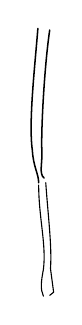
\begin{tikzpicture}[x=1mm,y=1mm,baseline=(current bounding box.center),line cap=round,line join=round]
\draw[line width=0.55pt] (0,34) .. controls (-0.4,29) and (-1.2,22) .. (-0.7,18.5) .. controls (-0.6,16.5) and (0.1,15.5) .. (0.1,14.4);
\draw[line width=0.40pt] (0.1,14.1) .. controls (0.1,10) and (1.1,6.5) .. (0.7,3.4) .. controls (0.4,1.8) and (0.3,0.9) .. (0.7,0);
\draw[line width=0.55pt] (1.5,33.8) .. controls (0.8,29) and (0.4,21) .. (0.5,18.5) .. controls (0.6,16.9) and (0.1,15.5) .. (0.8,15.0);
\draw[line width=0.40pt] (1.0,14.4) .. controls (1.3,10.1) and (1.8,6.3) .. (1.6,3.5) -- (2.0,0.5) -- (1.5,0.1);
\end{tikzpicture}}}

(On l'a établi tt au moins dans le cas
\(\Gamma=\Gamma^0\), il faudrait revenir sur le cas général,
je pense que ça reste vrai tel quel, à vérifier\ldots)
\margin{\figure{[Un trait vertical à gauche des deux lignes
« je pense \ldots{} vérifier\ldots) ».]}}
De plus, on vit apparaître une \uuline{structure supplémentaire}
sur le groupe \(\mathcal E\)
[qui dans le cas anabélien s'identifie à un sous-groupe de
\(\operatorname{Aut}(\pi)\)], à savoir une application
\[
\mu_{\mathcal E}:
\text{éléments }\inserted{u}\text{ d'ordre fini de }\mathcal E
\longrightarrow T\otimes\mathbb Q/\mathbb Z,
\]
\unsure{obtenue} en notant que si \(u\in\mathcal E\) est d'ordre fini
\(n\), \unsure{d'où} \(\mathbb Z/n\mathbb Z\lhook\joinrel\xrightarrow[i]{}
\mathcal E\), \unsure{on a|i.e.} \(\operatorname{Im}i\cap\pi=(1)\)
(\(\pi\) n'a pas d'éléments de torsion), donc
\(\mathbb Z/n\mathbb Z\hookrightarrow\Gamma\), \unsure{d'où|d'un} sous-groupe
\(\Gamma_1\subset\Gamma\) (i.e. l'image de
\margin{\uline{NB} Pour un \(u\) d'ordre fini de \(\mathcal E\),
on doit \unsure{savoir|avoir}, si \(u\notin\mathcal E^0\),
que \(u\) \unsure{est} d'ordre \(2\) exactement,
\illegible{5} pour \unsure{définir} \(\mu(u)\)!}

\margin{154}

\scanpage{156}

\(\unsure{u}\) dans \(\Gamma\) a \(\overline{\mathrm m}\) ordre \(n\)),
et le relèvement \(\Gamma_1\hookrightarrow\mathcal E\) définit un
\(x\in U^{\Gamma_1}\), \deleted{tel que} et \(u_1\) opérant sur \(U\)
en laissant fixe \(x\) correspond donc au voisinage de \(x\) à un
``multiplicateur'', qui (pour une orientation locale choisie) est une
racine primitive \unsure{\(n\).ième} de \(1\) i.e. un élément de
\(\mathbb Z/n\mathbb Z\), et qui pour orientation changeante
s'interprète intrinsèquement comme élément de
\(T\otimes\mathbb Z/n\mathbb Z
\subset T\otimes\mathbb Q/\mathbb Z\).

L'application \(\mu\) satisfait les conditions évidentes
\[
\begin{gathered}
\left\{
\begin{aligned}
\mu(\alpha u\alpha^{-1})&=\mu(u) &&\text{si }\alpha\in\pi\\
\mu(u^n)&=n\mu(u) &&\text{si }n\in\mathbb Z
\end{aligned}
\right.\\
\text{ordre }\mu(u)=\text{ordre de }u
\end{gathered}
\]
J'ignore si cette application \(\mu\) \deleted{est}
\inserted{peut se} définir intrinsèquement en termes de l'extension
\(\mathcal E\), ou si au contraire il peut exister deux extensions
\deleted{\unsure{iso}} \(\mathcal E,\mathcal E'\) de \(\Gamma\) par \(\pi\),
définies par des situations géométriques, de \(\Gamma\) opérant sur
\(U\) resp. \(U'\), et un isom. d'extensions
\(\mathcal E\longrightarrow\mathcal E'\) qui ne soit compatible avec
les fonctions \(\mu,\mu'\).
Le cas non trivial le plus simple à regarder est le cas

\margin{155}

\scanpage{157}
\mspage{78}

abélien (où \(\pi\simeq\mathbb Z\)
\inserted{\deleted{\illegible{1}} \((\operatorname{card}I=2)\)}
ou \(\pi\simeq\mathbb Z^2\) (\deleted{\unsure{card}} \(I=\varnothing\))),
Dans le \inserted{premier} cas
\deleted{d'une extension} \(\pi\simeq\mathbb Z\), \unsure{on|\deleted{les}}
\inserted{doit avoir (pour avoir une action fidèle de
\(\Gamma=\Gamma^0\))}
\deleted{extensions \illegible{1}}
\(\Gamma^0\) cyclique, \(\mathcal E\simeq\mathbb Z\),
il n'y a pas d'élément d'ordre fini dans \(\mathcal E\) sauf
\(\unsure{1|e}\), donc la question ne se pose pas.
Le cas \(\pi\simeq\mathbb Z^2\) est plus intéressant,
\deleted{\unsure{et peut se reformuler}}

Si \(\pi\) est un \(\mathbb Z\)-module libre de
\deleted{\unsure{t.f.}}\inserted{\unsure{rg \(n\)}}, on a une suite exacte
\diagram{
\begin{tikzcd}[ampersand replacement=\&,column sep=small,row sep=small]
0 \arrow[r] \& \pi \arrow[r] \& \pi\otimes_{\mathbb Z}\mathbb R
\arrow[r] \& X_0(\pi) \arrow[r] \arrow[d,dash] \& 0\\
\& \& \& \substack{\text{Tore de dim}\\ n\text{ associé à }\pi} \&
\end{tikzcd}
}
et si \(\Gamma\) opère sur \(\pi\), la suite exacte de cohomologie
(compte tenu de \(H^i(\Gamma,\pi\otimes_{\mathbb Z}\mathbb R)=0\)
pour \(i>0\)) donne
\diagram{
\begin{tikzcd}[ampersand replacement=\&,column sep=large,row sep=small]
H^2(\Gamma,\pi) \& H^1(\Gamma,X_0(\pi)) \arrow[l,"\sim" {anchor=south}]\\
\substack{\text{\unsure{classe d'extension|classes d'extensions}}\\
\text{de }\Gamma\text{ par }\pi}
\&
\substack{\text{classes de}\\X_0(\pi)\text{ torseurs,}\\
\text{avec op. de }\Gamma\text{ dessus}\\
\text{compatible avec son}\\\text{action sur }X_0(\pi)}
\end{tikzcd}
}

donc la donnée d'une extension \(\mathcal E\) de \(\Gamma\) par \(\pi\)
revient essentiellement à celle d'un
\unsure{\(\Gamma\)-\(X_0(\pi)\)-torseur} \(X\)
(\(n\)-tore inhomogène sur lequel \(\Gamma\) opère --- donc il opère
sur son groupe des translations \(X_0\), donc sur
\(\pi=\pi_1(X_0,0)\)\ldots).
S'il était vrai \inserted{pour \(n=2\)} que tte opération

\margin{156}

\scanpage{158}

de \(\Gamma\) sur une surface torique \((\simeq S^1\times S^1)\)
est isomorphe à une telle action standard, alors le caractère
intrinsèque de l'application \(\mu\) dans ce cas serait établi
--- ce qui ne \unsure{rendrait} pas inintéressant pour autant le calcul
de \(\mu\), qui prend ses valeurs dans
\(T\otimes\mathbb Q/\mathbb Z\), où ici
\[
T\simeq\bigwedge\nolimits_{\mathbb Z}^{2}\pi
\quad
(\text{\unsure{dual|dim.\ 2} de }H^2(\pi,\mathbb Z)\simeq
\bigwedge\nolimits^{2}
\underbrace{H^1(\pi,\mathbb Z)}_{
\substack{\unsure{\downarrow|\simeq}\\ \pi^\vee}}).
\]

La question revient à celle-ci : On a une extension \uline{scindée}
d'un \deleted{\unsure{groupe}}\inserted{\unsure{groupe}} cyclique
\(\mathbb Z/n\mathbb Z\) de générateur \(u\) par \(\pi\)
--- décrite donc entièrement par un autom.
\deleted{d'ordre} \(\unsure{\theta}\) de \(\pi\) tel que
\(\theta^n=\operatorname{id}_\pi\)), décrire \unsure{en} termes de
ceci un élément de \(T\otimes\mathbb Q/\mathbb Z\).

Réponse : la situation géométrique \unsure{standard|st. dont}
correspond à \(X=X_0(\pi)\), avec \(0\) comme pt fixe sous \(\Gamma\).
Si \(u\) renverse l'orientation, il est d'ordre \unsure{\(1\) ou|i.e.} \(2\),
il n'y a pas de Pb, sinon c'est \deleted{dans} en
\(\pi\otimes_{\mathbb Z}\mathbb R\) une rotation autour de \(0\)
(d'ordre \(2,3,4\) ou \(6\)) qui se repère bien par un élément
de \deleted{\illegible{1}} \(T\otimes\mathbb Z/\nu\mathbb Z\)
(si \(\nu\) est \unsure{d'ordre|l'ordre}).
C'est aussi (si on identifie
\(T\otimes\mathbb Z/\nu\mathbb Z\) à
\(\mu_\nu(\mathbb C^*)\), en supposant
\(T\simeq\mathbb Z\) donné
i.e. \(\pi\) orienté i.e. \(X_0(\pi)=\unsure{X}\)
orienté) \uline{une} des deux

\margin{157}

\scanpage{159}
\mspage{79}

valeurs propres de \(u\otimes_{\mathbb Z}\mathbb C\)
(autom du vectoriel sur \(\mathbb C\) de dim \(2\)
\(\pi\otimes_{\mathbb Z}\mathbb C\)).

Ceci nous montre, dans le cas de la géom Alg sur corps alg clos
\(\Omega\), que si \(X=X_0\) est une courbe elliptique
\(u\) un autom d'ordre fini, on a comme description
paradigmatique non \uline{seult}
\(\pi=\pi_1(X,0)\)
\inserted{(\(\widehat{\mathbb Z}\)-module libre de rg \(2\)),}
(et l'action de \(u\) sur \(\pi\)), mais comme structure
\uline{supplémentaire} l'une des deux solutions \uline{dans \(\Omega\)}
de l'équation caractéristique de \(u\) (à coefficients entiers)
\[
T^2+aT+b=0
\qquad (a=-\operatorname{Tr}u,\ b=\unsure{\det u}).
\]

Il est clair que cette structure supplémentaire ne peut se déduire
de la seule connaissance de l'action de \(u\) sur \(\pi\).
\margin{\figure{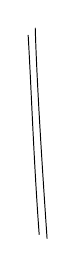
\begin{tikzpicture}[x=1mm,y=1mm,baseline=(current bounding box.center),line cap=round]
\draw[line width=0.35pt] (0,25.8) .. controls (0.4,19) and (0.7,10) .. (1.4,0.5);
\draw[line width=0.35pt] (0.9,26.7) .. controls (1.1,19.7) and (1.8,8.8) .. (2.4,0);
\end{tikzpicture}}
pour \(\unsure{\Omega}=\mathbb C\)
\illegible{2} \unsure{revient à}
\illegible{1} \uline{\unsure{orientation|orientations}} de
\illegible{1}}
Mais il reste la question si cette \deleted{\unsure{dernière}}
\inserted{\unsure{\(\mu(u)\in\mu_n^*(\Omega)\)}}
peut se déduire de la connaissance au moins de l'action
\inserted{extérieure} de \(u\) sur le groupe
``avec \(1\) lacet'' correspondant à la situation géométrique
--- i.e. un autom \inserted{ext.}
\deleted{\illegible{2}} d'ordre \(n\) \unsure{d'} un tel groupe
(ou si là encore il faut la considérer décidément comme une donnée
supplémentaire).
\margin{oui, il le peut, grâce à la considération des
``sous-groupes \illegible{2} de \(\mathcal E\)''
\illegible{2} qui définissent des extensions
\diagram{\begin{tikzcd}[ampersand replacement=\&,row sep=2.5em,column sep=2em]
\unsure{1} \arrow[r] \& T \arrow[r] \arrow[dr,dotted,no head,"\unsure{n_i\,\mathrm{id}_T}"'] \& \mathcal E_i \arrow[r] \arrow[d,phantom,"\simeq"{description,rotate=90}] \& \Gamma_i \arrow[r] \& 1 \\
\& \& T \& \&
\end{tikzcd}}
d'où \(\unsure{\Gamma_i\simeq T/n_iT}\)
\illegible{2}}
Mais s'il en était bien ainsi, cela impliquerait d'autre part que la
construction de \unsure{\(u\in\) groupe|ces groupes} à

\margin{158}

\scanpage{160}

(1) lacet(s), avec l'op. de \(\Gamma\) dessus, ne peut se faire non
plus à l'aide de la seule \deleted{\illegible{2}}
connaissance de l'action de \(\Gamma\) (\(=\mathbb Z/n\mathbb Z\))
sur \(\pi\).
C'est cette question de ``forage de trous'' qu'il faut donc en fin de
compte, à la fin des fins, attaquer !

Quant à la question de savoir si
\deleted{\illegible{1}}\inserted{dans}
\deleted{\illegible{1}} le \uline{cas anabélien},
l'application
\[
\mu:\underbrace{{}_\infty\mathcal E}_{
\substack{\text{\unsure{ens des}}\\
\text{\unsure{élémts}}\\
\text{d'ordre fini de }\mathcal E}}
\longrightarrow T\otimes\mathbb Q/\mathbb Z)
\]
est déductible de l'action de \(\Gamma\) sur \(\pi\)
[si elle est fidèle, \(\mathcal E\) s'identifie donc à un ss-groupe
de \(\operatorname{Autext}_{\unsure{\ell|l}}(\pi)\)
et on peut se demander si \(\mu\) n'est pas
\inserted{alors} définissable sur cet tt entier],
ou \unsure{c'est|si c'est} une donnée supplémentaire dont il faut disposer pour
reconstituer la situation géom. --- la question reste entière.
\margin{cela semble bien \unsure{ainsi}, compte tenu
\illegible{1} que pour \(\Gamma\) \uline{résoluble},
\illegible{3}, on sait \illegible{1}
que tte action \deleted{\illegible{1}} de \(\Gamma\) sur \(\pi\)
\illegible{3} \unsure{réaliser géométriquement}}

\textcircled{16}\quad
\uuline{Bouchage et forage de trous:}
\uline{Préliminaires} \unsure{toposiques} généraux

Considérons une situation
\diagram{
\begin{tikzcd}[ampersand replacement=\&]
B_{D^*} \arrow[r] \& B_U
\end{tikzcd}
}
(de topos multigaloisiens)
\margin{NB. une telle situation
\inserted{toposique \unsure{décrit}} \(2\)-fidlt les situations topologiques \((X,S)\),
ou \(U\), pourvu qu'aucune composante irréductible de \(U\)
ne soit \(\simeq S^2\) ---}

\margin{159}
\scanpage{161}
\mspage{80}
% Lignes 1--5 (continuation de la note marginale de la page précédente).
\illegible{2}, et \unsure{au} \deleted{\unsure{le}} fait qu'elles restent \inserted{très} proches du langage \unsure{et|\deleted{et}} de l'intuition topologique, elle est supérieure au $p^t$ de vue ``groupes à lacets'', qui correspond à l'appr. du calculatoire plutôt.)

% Lignes 5--16 : grand passage encadré et barré par des traits obliques.
\deleted{, donnons-nous \deleted{une partie sous topos} (\inserted{\unsure{néc$^t$.}}\unsure{ouvert}) $B_{D_1^*}$ de $B_{D^*}$ (correspondant à une partie $I_1$ de $I=\pi_0(B_{D^*})$) de sorte que
\[
 B_{D^*}\simeq B_{D_0^*}\amalg B_{D_1^*}
\]
\margin{($D_0^*$ correspond à la partie $I_0=I\setminus I_1$ de $I$)}
On a une décomposition analogue
\[
 B_D\simeq B_{D_0}\amalg B_{D_1}.
\]
\inserted{\unsure{déf.} $B_{\pi_0(D^*)}=B_S$}
Considérons le topos \unsure{$B_U'$} ``somme amalgamée'' de \deleted{\unsure{$B_U$}}
\diagram{\begin{tikzcd}[ampersand replacement=\&]
 \& B_{D_1^*}\arrow[dl]\arrow[dr] \& \& \\
 B_U \& \& B_D\arrow[r,leftrightarrow,"\unsure{\sim}"] \& B_S
\end{tikzcd}}
}

% Lignes 17--24.
Je m'aperçois qu'il me faut revenir sur les notations des \deleted{\illegible{1}} \inserted{divers} topos associés à une telle donnée. Mais je vais me guider sur la situation des n$^\circ$ .-- où on a un schéma régulier \inserted{$X$} de dim 1, un sous-schéma fermé \inserted{$S$} de dim 0, d'où $U=X-S$ --- dans ce cas \deleted{\illegible{2}} $\unsure{S_{\text{ét}}|X_{\text{ét}}}$ \textcircled{ne} peut se reconstituer à partir de $B_{D^*}$ comme $\unsure{B_{\pi_0 B_{D^*}}|B_I}$
\mspage{160}


\scanpage{162}
% Lignes 1--7.
avec $I=\pi_0(B_{D^*})$, il faut tenir compte des corps résiduels $k(s)$ $(s\in S)$ i.e. des groupes de Galois $\operatorname{Gal}(\overline{k(s)}/k(s))$. Donc il y a lieu de revenir à une situation de départ (qui est adaptée au cas \inserted{arithmético-}géométrique) de morphismes de topos \uuline{multigaloisiens}
\[
 (*)\qquad
 \diagram{\begin{tikzcd}[ampersand replacement=\&]
 \& B_{D^*}\arrow[dl,"\rho"']\arrow[dr,"\sigma"] \& \\
 B_U \& \& B_S
 \end{tikzcd}}
\]
% Lignes 8--14.
(Attention, on écrit $B_S$, non $B_D$, qui aura un autre sens), \uline{où} $\sigma$ \uline{induit un iso sur les} $\Pi_0$ [et est surjectif sur les $\operatorname{Hom}$]. Pour l'instant, on ne va faire aucune hypothèse particulière sur cette situation, qui pour $B_U$ connexe, et en termes des choix
% Lignes 15--23 : crochet et parenthèses tels que visibles.
[\deleted{d'objets $\widetilde D_i^*\in\unsure{D}$} de rev. universels $\widetilde D_i^*$ des comp. conn. $D_i^*$ de $D^*$, et d'un rev universel $\widetilde U$ de $B_U$, et de l'isom. entre les $\rho_!(\widetilde D_i^*)$ et $\widetilde U$) s'explicite par la donnée d'un groupe \inserted{$\mathcal E$ (ou} $\Pi$) $(=\operatorname{Aut}(\widetilde U))$ \deleted{\unsure{et}} \inserted{$\mathcal E_i$ (ou} $\Pi_i$ $(=\operatorname{Aut}(\widetilde D_i^*))$ \deleted{\illegible{2}} $(i\in I)$, $\Gamma_i$ $(i\in I)$
\mspage{161}


\scanpage{163}
\mspage{81}
% Lignes 1--3 et premier diagramme.
et des homomorphismes de groupes
\diagram{\begin{tikzcd}[ampersand replacement=\&,row sep=2em,column sep=2.5em]
\& \unsure{\mathcal E_i} \arrow[dl,no head,"\rho_i"'] \arrow[dr,"\sigma_i"] \& \\
\unsure{\mathcal E} \& \& \Gamma_i
\end{tikzcd}}
avec les $\sigma_i$ surjectifs. \deleted{\unsure{et}}
% Lignes 3--10.
[Quand il y a un corps de base $K$ pour la situation géométrique, alors ds la description \unsure{toposienne}, \inserted{\unsure{posant} $e=\operatorname{Spec}K$ et} désignant par $B_e$ le topos étale \inserted{$e_{\text{ét}}$} de $e$, i.e. $B_\Gamma$ \unsure{où|si} $\Gamma=\operatorname{Gal}(\overline K/K)$, le diagramme $*$ s'insère dans
\diagram{\begin{tikzcd}[ampersand replacement=\&]
 \& B_{D^*}\arrow[dl,"\rho"']\arrow[dr,"\sigma"] \& \\
 B_U\arrow[dr,"\varphi"'] \& \& B_S\arrow[dl,"\psi"] \\
 \& B_e \&
\end{tikzcd}},
avec donnée de commutativité pour le carré envisagé\unsure{\ldots\ comme envisagé} au début de ces notes].

% Lignes 11--18 et dernier diagramme.
En termes de $*$, on construit par ``recollement'' de $B_U$ et \inserted{de} $B_S$ (via le foncteur de recollement $\sigma_*\rho^*$) un topos mixte, qui n'est plus en général multigaloisien, noté précédemment $\unsure{D_{X,U}|B_{X,U}}$, et que \inserted{\unsure{je préfère}} maintenant \deleted{\illegible{1}} \unsure{noter|notés} $B_{X;S}$ \deleted{\illegible{2}} \inserted{[pour rappeler qu'il s'agit de faisceaux sur $X$, mais n'ayant de singularités que sur $S$]} \deleted{\illegible{1} s'insère dans un}. Il s'insère dans un diagramme de topos
\diagram{\begin{tikzcd}[ampersand replacement=\&,row sep=2em,column sep=2.5em]
\& B_{D^*} \arrow[dl] \arrow[dr] \& \\
B_U \arrow[dr,""{name=xl,description}] \& \& B_S \arrow[dl,""{name=xr,description}] \\
\& B_{X;S} \&
\arrow[from=xr,to=xl,bend right=25,"\alpha_X"]
\end{tikzcd}}
avec une flèche
\mspage{162}


\scanpage{164}
% Lignes 1--5.
``de commutation'' $\alpha$ qui n'est telle que par abus de langage --- ce n'est pas un iso \deleted{de \unsure{foncteurs}} mais un morphisme de foncteurs sans plus
\[
 \sigma^*\psi^*\deleted{\unsure{u}}\xrightarrow{\alpha_X}\rho^*\varphi^*.
\]
% Lignes 6--11.
De la $\overline{\mathrm m}$ façon, recollant $D^*$ et $S$ via $\sigma_*$ (i.e. remplaçant $B_U$ par $B_{D^*}$ dans la construction précédente de $\unsure{D_{X;S}|B_{X;S}}$), on trouve un topos, pas multigaloisien en général, noté $B_{D;S}$. Dans le \deleted{\unsure{présent}} modèle géométrique où on a $X,S$ comme dessus,
% Lignes 12--18.
$B_X$ correspond aux faisceaux sur $X$ qui sont \unsure{ess.|ens.|en.} loc. constants sur $U$ (et sur $S$, où ils n'ont pas de mérite) i.e. sur $U$ proviennent par l'image inverse \deleted{d'un faisceau} \inserted{par} $U\longrightarrow B_{\Pi_1 U}$ d'un faisceau sur $B_{\Pi_1 U}$.

% Lignes 19--25.
et de $\overline{\mathrm m}$ $B_{D;S}$ correspond aux faisceaux sur $D=\coprod_i\operatorname{Spec}(\mathcal O_i=\text{hensélisé de }\mathcal O_{X,\unsure{i|s}})$ \deleted{qui sont} qui sont loc constants sur $D^*=D-S$ (et sur $S$, sans mérite!) mais avec l'hyp. de dim faite -- --- \unsure{en|on} fait
\[
 B_{D;S}\simeq D_{\text{ét}}
\]
($D_i$ n'a que 2 pts, $D_i^*=\{\eta_i\}$ --- ). Ainsi $B_{D;S}$ \unsure{$(\simeq D_{\text{ét}})$}
\mspage{163}


\scanpage{165}
\mspage{82}
% Lignes 1--2 et diagramme supérieur.
(quand on part de $X,S$) s'insère dans un triangle de morphismes de topos
\diagram{\begin{tikzcd}[ampersand replacement=\&,row sep=2em,column sep=2.5em]
\& B_{D^*} \arrow[dl,equals,""{name=deq,description}] \arrow[dr,"\sigma",""{name=dsig,description}] \& \\
B_{D^*} \arrow[dr,"\varphi_D"'] \& \& B_S \arrow[dl,"\psi_D"] \\
\& B_{D;S} \&
\arrow[from=dsig,to=deq,bend left=22,"\alpha_D"']
\end{tikzcd}}
\margin{\uline{NB} dans le cas géométrique, \deleted{\illegible{1}} \unsure{trois} topos de ce diagramme sont des topos étales ($D^*_{\text{ét}},D_{\text{ét}},S_{\text{ét}}$) et les flèches $\varphi_D$ et $\psi_D$ correspondent à \unsure{des morph.} \unsure{mais non} \illegible{1} de topos)}
% Lignes 3--4.
$\alpha_D$, comme $\alpha_X$ ci-dessus, n'est qu'un vulgaire homom. (pas iso en général).

% Lignes 5--14.
\deleted{On trouve donc un \unsure{to.}}
Quand on parle du morphisme canonique de $B_{D^*}$ dans $B_{D;S}$ c'est \inserted{de} $\varphi_D$ (et non de $\psi_D\sigma$) qu'il s'agit --- dans le cas géométrique on a $B_{D^*}\simeq D^*_{\text{ét}}$, et $\varphi_D$ correspond à l'inclusion de schémas
\[
 D^*\unsure{\supset|=}D\setminus S\longrightarrow D
\]
\inserted{et $\psi_D:B_S\longrightarrow B_{D;S}$ à l'inclusion de schémas $S\longrightarrow D$}
alors que $\sigma$ ni $\psi_D\sigma$ ne correspondent en général à des morphismes de schémas.

% Lignes 15--16 et diagramme inférieur entièrement barré.
On obtient ainsi un diagramme de topos
\deleted{\diagram{\begin{tikzcd}[ampersand replacement=\&,row sep=3em,column sep=4em]
\& B_{D^*}
\arrow[dl,"\unsure{\rho_X}"',"\deleted{\unsure{B_{D^*}}}"{description,pos=0.56},"\deleted{\unsure{\varphi_D}}"{pos=0.25}]
\arrow[dl,bend right=38,"\deleted{\unsure{\illegible{1}}}"']
\arrow[dr,"\sigma"{xshift=0.65em,yshift=0.55em}]
\arrow[d] \& \\
B_U \arrow[dr,"\varphi"',""{name=oldl,description}] \& B_D \arrow[d] \& B_S \arrow[l] \arrow[dl,"\psi",""{name=oldr,description}] \\
\& B_X \&
\arrow[from=2-1,to=2-2,phantom,"\text{comm}"{description,yshift=1.3em}]
\arrow[from=1-2,to=2-3,phantom,"{\begin{gathered}\text{pseudo-}\\[-0.4ex]\text{comm}\end{gathered}}"'{pos=0.65,xshift=-1.9em,yshift=-0.5em}]
\arrow[from=2-2,to=2-3,phantom,"\text{comm}"{description,yshift=-1.3em}]
\arrow[from=oldr,to=oldl,bend right=20,"\deleted{\unsure{\illegible{1}}}"]
\end{tikzcd}}
où dans le cas géométrique}
\mspage{164}


\scanpage{166}
% Diagramme supérieur (**).
\[
 (**)\qquad
 \diagram{\begin{tikzcd}[ampersand replacement=\&, column sep=large,row sep=small]
 \& \& \uline{B}_S\arrow[dl]\arrow[dd,"{\Vert}" description] \\
 \uline{B}_{D^*}\arrow[r]\arrow[dd]\arrow[urr] \& B_{D;S}\arrow[dd] \& \\
 \& \& \uline{B}_S\arrow[dl] \\
 \uline{B}_{\unsure{U}}\arrow[r] \& B_{X;S} \&
 \end{tikzcd}}
\]
\margin{Attention, le triangle n'est pas ess. commutatif, mais \unsure{on a} pseudo-commutativité\ldots}
% Lignes 1--5.
où les trois topos soulignés $\uline{B}_U$, $\uline{B}_S$ et $\uline{B}_{D^*}$ sont multigaloisiens, et $B_{D;S}$ et $B_{X;S}$ sont composites (obtenus par recollement de deux topos multigaloisiens).
\inserted{Sauf erreur les deux carrés sont [\uline{non} seulement ess$^t$. comm. mais aussi] 2-cartésiens (dans la 2-cat. des topos).}

% Lignes 6--12 et diagramme médian.
Passant aux $B_{\Pi_1}$? des topos envisagés (correspondants aux objets loc. constants sur ces topos) on trouve \inserted{un topos} $B_{\deleted{\Pi_1}X}$ \inserted{$=\unsure{B_{\Pi_1 B_{X,S}}|B_{\Pi_1 B_{X;S}}}$} comme somme amalgamée de topos dans le \deleted{$B_{\Pi_1 X}$} diagramme
\diagram{\begin{tikzcd}[ampersand replacement=\&,row sep=2em,column sep=2.5em]
\& B_{D^*} \arrow[dl] \arrow[dr] \& \\
B_U \arrow[dr,""{name=pl,description}] \& \& B_S \arrow[dl,no head,""{name=pr,description}] \\
\& B_{\deleted{\unsure{\Pi_1}}X} \&
\arrow[from=pr,to=pl,bend right=25,"\sim"]
\end{tikzcd}}
% Lignes 13--19.
(ce carré est bel et bien essentiellement commutatif) et de $\overline{\mathrm m}$ (remplaçant $B_U$ par $B_{D^*}$) un $B_{\deleted{\Pi_1}D}$, qui est cependant (par $B_S\longrightarrow B_{\deleted{\Pi_1}D}$) isom. \inserted{(plutôt: \unsure{équiv.|égaux})} à $B_S$. Le diagramme $(**)$ devient alors
\mspage{165}


\scanpage{167}
\mspage{83}
% Diagramme supérieur (***).
\[
 (***)\qquad
 \diagram{\begin{tikzcd}[ampersand replacement=\&, column sep=large,row sep=small]
 \& \& B_S\;(=B_{\Pi_1 S})\arrow[dl,"\sim"']\arrow[dd,"{\Vert}" description] \\
 B_{D^*}\;(=B_{\Pi_1 D^*})\arrow[r]\arrow[dd]\arrow[urr,"\sigma"] \& B_{\deleted{\Pi_1}D}\arrow[dd] \& \\
 \& \& B_S\arrow[dl] \\
 B_U\;(=B_{\Pi_1 U})\arrow[r] \& B_{\deleted{\Pi_1}X} \&
 \end{tikzcd}}
\]
% Lignes 1--4.
où cette fois-ci le triangle sup. est bien ess. surjectif (c'est bien comme ça qu'on a défini $\sigma$, dans le cas géométrique!) et on a un morphisme de
% Lignes 5--12.
$(**)$ dans $(***)$, qui \deleted{\unsure{est}} pour les flèches qui \unsure{n'sont|sont} pas ess. des \inserted{\unsure{(semi-}}identités), $B_{D;S}\longrightarrow B_{\deleted{\Pi_1}D}$ et $B_{X;S}\longrightarrow B_{\deleted{\Pi_1}X}$, ont une nette tendance d'être ``acycliques'' i.e. d'induire des iso. sur la cohomologie (il faudrait voir \illegible{1} ce point). Enfin,
% Lignes 13--15 et diagramme inférieur (****).
dans le cas géométrique, on a \inserted{\unsure{des}} diagrammes \unsure{analogues|canoniques} de morphismes de topos étales \deleted{\illegible{1}}
\[
 (****)\qquad
 \diagram{\begin{tikzcd}[ampersand replacement=\&, column sep=large,row sep=small]
 \& \& S_{\text{ét}}\arrow[dl]\arrow[dd,equal] \\
 D^*_{\text{ét}}\arrow[r]\arrow[dd]\arrow[urr] \& D_{\text{ét}}\arrow[dd] \& \\
 \& \& S_{\text{ét}}\arrow[dl] \\
 U_{\text{ét}} \& X_{\text{ét}}\arrow[l] \&
 \end{tikzcd}}
\]
\margin{triangle sup. pas ess. comm.}
\mspage{166}


\scanpage{168}
% Lignes 1--2.
où toutes les flèches sauf $D^*_{\text{ét}}\longrightarrow S_{\text{ét}}$ sont induites par des morphismes de topos.
% Lignes 3--11.
Ici $(****)$ s'envoie dans le diagramme homologue $(**)$, en induisant des iso. de topos pour $D^*,D,S$, et pour $U_{\text{ét}}\longrightarrow B_U$ et $X_{\text{ét}}\longrightarrow X$ induisant des morphismes qui ont moins tendance d'être acycliques, mais qui le sont \deleted{\unsure{cependant}} quand $\overline{\mathrm m}$ dans des cas importants, rappelés dans une section antérieure\ldots

% Lignes 12--15 et diagramme.
Les constructions de $(**)$ et $(***)$ en termes du diagramme de départ
\diagram{\begin{tikzcd}[ampersand replacement=\&]
 \& B_{D^*}\arrow[dl]\arrow[dr] \& \\
 B_U \& \& B_S
\end{tikzcd}}
sont purement formelles, et indépendantes de \unsure{tte} hypothèse.
% Lignes 16--22.
La construction d'un $B_{\deleted{\Pi_1}X}$ multigaloisien, comme somme amalgamée, peut être interprété comme la traduction (au niveau des groupoïdes fondamentaux) d'une opération de ``bouchage de trous''.
\deleted{Au niveau} Dans le contexte calculatoire
\mspage{167}


\scanpage{169}
\mspage{84}
% Ligne 1 et diagramme de groupes.
(avec choix des $\widetilde U,\widetilde U_i$, $\rho_!(\widetilde U_i)\simeq\widetilde U$) on a
\diagram{\begin{tikzcd}[ampersand replacement=\&]
 \& \mathcal E_i\arrow[dl,"\rho_i"']\arrow[dr,"\sigma_i"] \& \\
 \pi \& \& \Gamma_i
\end{tikzcd}},
% Lignes 2--8.
posant $\widetilde X=\text{image de }\widetilde U$ par $i_!$ $(i:B_U\longrightarrow B_{\Pi_1 X})$ $B_{\deleted{\Pi_1}X}$ est décrit en termes de ce $\widetilde U$ comme le \deleted{topos des $\Pi$-ens} classifiant $B_{\pi_X}$, où $\pi_X=\pi_1(X;\widetilde X)$ \deleted{est défini} \inserted{se calcule} comme quotient de $\pi$ par le ss-groupe invariant engendré par les $\rho_i(L_i)$, où $L_i=\operatorname{Ker}\sigma_i\subset\mathcal E_i$.

% Lignes 9--16.
Si on se donne un sommande direct $B_{D_0^*}$ de $B_{D^*}$ (correspondant à une partie $I_0$ de $I=\pi_0(B_{D^*})$) on trouve de $\overline{\mathrm m}$ une somme amalgamée de $B_U$ et de $B_{S_0}$ sous $B_{D_0^*}$, noté \deleted{$\unsure{B_{\Pi_1(U\cup S_0)}}$} \inserted{$B_{U\cup S_1}\longleftarrow B_U$}, qui se visualise comme un bouchage partiel de trous, interprété au niveau des groupoïdes fondamentaux. Dans le cas géom, si on pose $I=I_0\amalg I_1$, i.e. $S=S_0\amalg S_1$, on
\mspage{168}


\scanpage{170}
% Lignes 1--2.
peut interpréter ce topos comme $B_{\Pi_1 U_1}$, où $U_1=X\setminus\unsure{S_1}$. \deleted{Bien sûr,}

% Lignes 3--6 et premier petit diagramme.
Bien sûr, on a un hom de diagrammes cocartésiens de topos relatif à
\diagram{\begin{tikzcd}[ampersand replacement=\&]
 \& B_{D_0^*}\arrow[dl]\arrow[dr] \& \\
 B_U \& \& B_{S_0}
\end{tikzcd}}
\deleted{\unsure{de dessous}} celui relatif à $B_{D^*}$ \deleted{\unsure{la situation}} s'envoyant dans $B_U$, et \deleted{$\unsure{B_{S_0}}$} $B_S$
% Grand diagramme central, avec surcharges et traits peu lisibles.
\diagram{\begin{tikzcd}[ampersand replacement=\&,row sep=3em,column sep=1.3em]
[B_{D_1^*}] \arrow[dr,dotted] \& \& B_{D_0^*} \arrow[dl] \arrow[dr] \arrow[rrr] \& \& \& B_{D^*} \arrow[dl,phantom,""{name=diagupper,description,pos=0.68,inner sep=0pt},""{name=diaglower,description,pos=0.86,inner sep=0pt}] \arrow[dr] \& \\
\& |[alias=leftU]| B_U \arrow[dr] \arrow[rrr,phantom,""{name=ugapleft,description,pos=0.39},""{name=ugapright,description,pos=0.76},""{name=utip,description,pos=0.88},""{name=uheadstart,description,pos=0.93,inner sep=0pt},""{name=uheadend,description,pos=0.97,inner sep=0pt},""{name=udashleft,description,pos=0.74,yshift=2pt,inner sep=0pt},""{name=udashright,description,pos=0.80,yshift=2pt,inner sep=0pt}] \& \& |[yshift=1.5em]| B_{S_0} \arrow[dl] \arrow[rrr] \& |[alias=rightU]| B_U \arrow[dr] \& \& |[yshift=1.5em]| B_S \arrow[dl] \\
\& \& B_{\deleted{\unsure{\Pi_1}}(\underbrace{U\cup S_0}_{U_1})} \arrow[rrr,no head] \& \& \&
\begin{gathered}
B_{\deleted{\unsure{\Pi_1}}(\underbrace{U\cup S}_{X})}\,\unsure{'}\\[-0.2ex]
\deleted{\unsure{\illegible{1}}\;B_{\unsure{\Pi_1}X}}
\end{gathered} \&
\arrow[from=1-6,to=diagupper,no head,shorten >=0pt]
\arrow[from=diaglower,to=rightU,no head,shorten <=0pt]
\arrow[from=leftU,to=ugapleft]
\arrow[from=ugapright,to=utip,no head]
\arrow[from=uheadstart,to=uheadend,shorten <=0pt,shorten >=0pt]
\arrow[from=udashleft,to=udashright,no head,shorten <=0pt,shorten >=0pt]
\end{tikzcd}}
,
% Lignes 7--9.
et d'autre part on a \inserted{un composé} $B_{D_1^*}\longrightarrow B_U\longrightarrow B_{\deleted{\Pi_1}U_1}$ qui avec $\unsure{B_{D_1^*}}\longrightarrow B_{S_1}$ \deleted{peut être utilisé} \inserted{donne un diagramme} de topos
\diagram{\begin{tikzcd}[ampersand replacement=\&]
 \& B_{D_1^*}\arrow[dl]\arrow[dr] \& \\
 B_{\deleted{\Pi_1}U_1} \& \& B_{S_1}
\end{tikzcd}}
% Lignes 10--15 (phrase continuée hors du lot).
de $\overline{\mathrm m}$ type qu'au début, qu'on peut utiliser pour construire encore une \deleted{\unsure{donc|dans}} somme amalgamée. Et il est évident que celle-ci est can. équivalente à $B_{\deleted{\Pi_1}X}$, la somme amalgamée corres-
\mspage{169}
\scanpage{171}
\mspage{85}
% L01
pondant à cette intuition de départ...

% L02--L17: passage cancelled by long diagonal strokes; local cancellations retained.
\deleted{Critique des notations. Alors que les \deleted{\unsure{lettres}}
\unsure{graphismes} $B_U$, $B_X$ se construisent en
termes des lettres $U,X$ (\unsure{suggérant|s'agissant}, \unsure{en}
\unsure{l'espèce|l'origine}, des \unsure{schémas} $U,X$) de la
$\overline{\mathrm m}$ façon, ils ont des significations
bien différentes --- $B_U$ désigne le topos
\unsure{classifiant} $B_{\unsure{\Pi_1|\pi_1},U}$, mais $B_X$ un topos
nettement plus gros. Donc je préfère
écrire \deleted{\illegible{1}} \unsure{finalement} $B_{X;S}$ (pour suggérer
les faisceaux sur $X$ \unsure{ens.|ess.} constants sur
$X\setminus S$ et sur $S$) \deleted{\unsure{ou mieux}, $B_{U,S}$ (pour
\unsure{suggérer} un topos obtenu par recollement
de $U$ et $S$, de $\overline{\mathrm m}$ $B$} \inserted{et de $\overline{\mathrm m}$ $B_{D;S}$} ; par contre
dans $B_{\unsure{\Pi_1|\pi_1},D}$ et $B_{\unsure{\Pi_1|\pi_1},X}$ on écrirait
simplement (comme pour $B_U$)
\inserted{$B_D$, $B_X$}}

% L18--L23
Toutes ces opérations sont essentiellement
triviales et sans mystère, et indépendantes de
\unsure{ttes|les} hypothèses spéciales du type ``groupes à
lacets''. Un intérêt particulier s'attache
au cas où \unsure{$B_S$|$B_D$} est un topos discret i.e.
s'identifie à $B_I$, \deleted{\unsure{où}} $I=\pi_0(B_{D^*})$, de

% P: handwritten numeral in the lower-left corner; hand not identified.
\margin{170}

\scanpage{172}
% L01--L07
sorte qu'on part simplement d'un morphisme
de topos multigaloisiens
\[
 B_{D^*}\longrightarrow B_U
\]
mais où de plus on a un groupe $\Gamma$
\inserted{(discret, disons --- ou profini dans le \unsure{contexte}
\unsure{arithmétique})}
qui opère sur $B_{D^*}$, $B_U$ ; le morphisme
précédent commutant à l'action de $\Gamma$.

% L08--L13
Notons que la donnée d'une action
de $\Gamma$ sur un topos $B$ permet de
construire un topos $(B,\Gamma)$, et
un morphisme $(B,\Gamma)\longrightarrow B_\Gamma$
\inserted{(topos classifiant de $\Gamma$}
\uuline{i.e.} un $\Gamma$-torseur de $(B,\Gamma)$ --- et

% L14--L23
$B$ s'identifie au topos induit par
$\mathcal X=(B/\Gamma)$ sur ce $\Gamma$ torseur. Inversement,
la donnée d'un topos $\mathcal X$ et d'un
$\Gamma$-torseur $U$ de $\mathcal X$, et d'un
\unsure{isom.} de $B$ avec le topos induit
$\mathcal X_{/U}$, \deleted{\unsure{par}} (identifié à $U$, ou à $B$) permet
de récupérer des op. de $\Gamma$ sur $B$,
via les op. sur $U$. Donc, la \uline{donnée}

% P: handwritten numeral in the lower-left corner; hand not identified.
\margin{171}

\scanpage{173}
\mspage{86}
% L01--L08
 d'une op. de $\Gamma$ sur un topos \inserted{$B$} revient
à celle de la donnée de $B$ comme
rev. galoisien de groupe $\Gamma$ d'un
autre topos (\unsure{ess\textsuperscript{t}} unique, noté alors
$(B,\Gamma)$ ... ). Ainsi, faire opérer
\deleted{\unsure{$B_{D^*}$}} $\Gamma$ sur $B_{D^*}\longrightarrow B_U$, c'est
la $\overline{\mathrm m}$ chose que d'insérer cette
\deleted{\unsure{diagramme}} \inserted{flèche} dans un diagramme comme

% D01
\diagram{\begin{tikzcd}[ampersand replacement=\&]
 B_{D^*}\text{\deleted{\unsure{,\Gamma}}} \arrow[r] \arrow[d] \& B_U \arrow[d] \\
 B_{D^*,\Gamma} \arrow[r] \& B_{U,\Gamma}
\end{tikzcd}}

% L09--L14
 où les flèches verticales sont $\Gamma$-galoisiennes
et le carré est $2$-cartésien, ou encore
(indépendamment de la donnée préalable
de $B_{D^*}$, $B_U$) c'est se donner un
triangle \unsure{ess\textsuperscript{t}} commutatif de morphismes
de topos

% D02
\diagram{\begin{tikzcd}[ampersand replacement=\&,column sep=2.8em,row sep=2.6em]
B_{D^*,\Gamma} \arrow[rr] \arrow[dr] \& {} \& B_{U,\Gamma} \arrow[dl,no head] \\
{} \& B_{\Gamma} \& {}
\end{tikzcd}}

% P: handwritten numeral in the lower-left corner; hand not identified.
\margin{172}

\scanpage{174}
% L01--L07
Si $\Gamma$ opère sur un topos multigaloisien,
on voit que $(B,\Gamma)$ est aussi
multigaloisien, et la situation d'un
topos multigaloisien $B_U$ et d'une
opération de $\Gamma$ dessus, revient à celle
d'un topos multigaloisien \inserted{$B_{U,\Gamma}$} et d'
un morphisme $B_{U,\Gamma}\unsure{\longrightarrow|\longleftrightarrow}B_\Gamma$.

% L08--L12
Donc la donnée d'une situation
$B_{D^*}\longrightarrow B_U$ de topos multigal,
et d'une op. de $\Gamma$ dessus,
revient \unsure{ex.act} à celle d'\unsure{hom}
de topos multigaloisiens
\[
 B_{D^*,\Gamma}\longrightarrow B_{U,\Gamma}\longrightarrow B_\Gamma
\]

% L13--L16
\unsure{\deleted{La connexité}|\uline{La connexité}}
$B_{U,\Gamma}$ est \unsure{$0$-conn.} ssi $\operatorname{card}\pi_0(\unsure{B_U})/\Gamma=1$,
i.e. $B_U$ non vide et $\Gamma$ transitif sur
$\pi_0(B_U)$. --- Notons que la situation

% P: handwritten numeral in the lower-left corner; hand not identified.
\margin{173}

\scanpage{175}
\mspage{87}
% L01--L11
 envisagée au début, avec $(X,S)$ sur corps $K$,
d'où \deleted{\unsure{$B$}} $B_{D^*}\longrightarrow B_U\longrightarrow B_\Gamma$
\inserted{``$e_{\text{ét}}$}
$(\Gamma=\operatorname{Gal}(\overline K/K))$
peut être interprétée comme déduite
de la situation ``géométrique'' $(\overline X,\overline S)$ sur $\overline K$,
ou $B_{\overline D^*}\longrightarrow B_{\overline U}$, en tenant compte
des opérations de $\Gamma$ dessus. Il se trouve
que pour beaucoup de questions, c'est
cette interprétation ``géométrique'' (au
sens strict, i.e. sur $\overline K$ alg. clos) avec
opérations d'un groupe de Galois $\Gamma$, qui
est la plus commode.

% L12--L23
Si on regarde une opération de $\Gamma$
sur un topos ($B_{D^*}$ disons),
il opère sur le topos discret $B_{\unsure{I|\pi_0}}$
$(I=\pi_0(B_{D^*}))$, et $B_{D^*}\longrightarrow B_I$ est
compatible aux actions de $\Gamma$. \deleted{\unsure{En}}
Mais le \deleted{structure de} \inserted{topos} $B_{(I,\Gamma)}$ est aussi
celui des $\Gamma$-ensembles au dessus de
$I$ (sur lequel $\Gamma$ opère) --- un topos induit
de $B_\Gamma$ --- \deleted{et les \unsure{fibres au-dessus}
d'un $i\in I$ \unsure{de}} \inserted{ses composantes}
connexes correspondent

% P: handwritten numeral in the lower-left corner; hand not identified.
\margin{174}

\scanpage{176}
% L01--L05
aux orbites de $\Gamma$ sur $I$. Si $\Gamma$ est
transitif sur $I$ \inserted{non vide} (ou si on regarde \uline{une}
telle orbite...), choisissant $i\in I$, le topos
en question s'identifie à $B_{\Gamma_i}$, où $\Gamma_i$
est le \unsure{Stabilisateur} de \deleted{\illegible{1}} $i$ dans $\Gamma$.

% L06--L16
\uline{NB} Se donner une opération de $\Gamma$
sur un topos \uline{discret} $B$ ($=B_I$),
quand on l'interprète en tant
que morphisme d'un topos
multigaloisien $B'=(B,\Gamma)\longrightarrow B_\Gamma$,
est caractérisé par le fait que
le morphisme \inserted{\unsure{de groupoïdes qui le décrit}}
soit \uline{injectif} sur les
flèches, i.e. en termes d'un \unsure{système}
\unsure{d'hom.} de groupes $\Gamma_j\longrightarrow\Gamma$ ($j\in J$
$[\simeq I/\Gamma]$), par la condition que ces
homs soient injectifs. [et alors $I$

% L17--L20
se reconstitue comme la somme
directe des $\Gamma/\Gamma_j$ ... ]. Ainsi un
diagramme
\[
 B_{D^*}\longrightarrow B_U
\]

% P: handwritten numeral in the lower-left corner; hand not identified.
\margin{175}

\scanpage{177}
\mspage{88}
% L01--L08
\uline{avec action de $\Gamma$} équivaut à la donnée
d'un diagramme
\[
 B_{D^*,\Gamma}\longrightarrow B_{U,\Gamma}\longrightarrow B_\Gamma
\]
et celui se complète (en utilisant
l'action de $\Gamma$ sur $\pi_0(B_{D^*}]$ ---
$B_{D^*}$ étant lui $\overline{\mathrm m}$ déduit de $B_{D^*,\Gamma}\longrightarrow B_\Gamma$
comme l'image inverse du torseur
universel) \deleted{\unsure{comme|avec}} en
\[
 B_{D^*,\Gamma}\longrightarrow B_{I,\Gamma}\longrightarrow B_\Gamma
\]

% L09--L16
 où $B_{D^*,\Gamma}\longrightarrow B_{I,\Gamma}$ peut aussi se
décrire directement en termes de
$B_{D^*,\Gamma}\longrightarrow B_\Gamma$ (comme dans un n\textsuperscript{o}
antérieur), \inserted{au niveau des groupoïdes fondamentaux,}
par un passage au
quotient, \unsure{dans|des} chaque \unsure{composante connexe|composantes connexes}
de $\Pi_1 B_{D^*,\Gamma}$, par les noyaux des applications
\unsure{sur les homs déduites|par les homs déduites} de $\Pi_1 B_{D^*,\Gamma}\longrightarrow\Pi_1 B_\Gamma$.

% L17--L20
--- i.e. il s'agit de la factorisation
canonique d'un hom de \unsure{g-poïdes|groupoïdes}
en \unsure{(}\inserted{\unsure{bi|bij} (pour objets),} épi
\deleted{(pour \illegible{1})} \inserted{(pour hom)}\unsure{)} suivi de \unsure{mono}
(pour hom). On trouve ainsi un

% P: handwritten numeral in the lower-left corner; hand not identified.
\margin{176}

\scanpage{178}
% L01; D01
carré essentiellement commutatif
\diagram{\begin{tikzcd}[ampersand replacement=\&]
 \& B_{D^*,\Gamma} \arrow[dl] \arrow[dr] \& \\
 B_{U,\Gamma} \arrow[dr] \& \& B_{I,\Gamma} \arrow[dl] \\
 \& B_\Gamma \&
\end{tikzcd}}

% L02--L03; D02
qui \deleted{\unsure{n'est autre que celui que}}
\inserted{correspond au diagramme de groupoïdes}
au début des notes \deleted{\unsure{que}} \deleted{\unsure{$\Pi$}} \deleted{\unsure{fait}} ($\S\,7$)
\diagram{\begin{tikzcd}[ampersand replacement=\&]
 \& \Pi_{D^*} \arrow[dl] \arrow[dr] \& \\
 \Pi_U \arrow[dr] \& \& \Pi_D \arrow[dl] \\
 \& \Pi_e \&
\end{tikzcd}}

% L04--L12
J'ai l'impression d'avoir à peu près
compris le mécanisme des actions des
groupes sur des topos multigaloisiens,
et comment \deleted{\unsure{celle-ci commute}}
\inserted{l'opération de passage}
d'un topos $B$ avec opération de $\Gamma$
au topos ``quotient'' $(B,\Gamma)=\text{``}B/\Gamma\text{''}$,
commute aux opérations du type
passage de
\diagram{[$B_{D^*}\longrightarrow B_U$ ; sous $B_{D^*}$,
$B_S$, relié à $B_{D^*}$ par un court trait vertical plus épais à son
extrémité inférieure : \unsure{flèche $B_{D^*}\to B_S$|renvoi d'insertion}.]}
à un $B_{X,S}$, via un
$B_X$ (``bouchage des trous''). \deleted{\unsure{Je}} Le temps

% P: handwritten numeral in the lower-left corner; hand not identified.
\margin{177}

\scanpage{179}
\mspage{89}
% L01--L03
semble donc mûr enfin pour s'expliquer
\unsure{sur|avec} l'opération inverse hypothétique
de ``forage \unsure{de|des} trous''.

% L04--L05
\unsure{17.} Complément sur les op. de groupes finis
sur les surfaces. (Complément au \unsure{$\S\,7$|$\S\,15$})

% L06--L12
Soit $U$ surface paracompacte connexe \unsure{!}
telle que $\pi_1(U)\ne(1)$ i.e. $U\not\simeq S^2,\mathbb R^2$.
On dit que $U$ est ``\unsure{anabélienne}'' si
$\pi$ non abélien (auquel cas $\operatorname{Centre}(\pi)=1$),
\unsure{i.e.|et} si $U\not\simeq\mathbb C^*,S^1\times S^1$.
Soit $\Gamma$
un groupe fini opérant sur $U$. Conditions
équivalentes :

% L13--L16
\unsure{b)|a)} \deleted{Pour} $\forall g\in\Gamma$, $g_U$ est isotope à l'identité.

$b')$ $\forall g\in\Gamma$, $g_U$ est homotope à l'identité.

$c)$ L'opération extérieure de $\Gamma$ sur
$\pi_1(U)$ est triviale.

% L17--L20
$d)$ \inserted{(cas anabélien)} L'extension $\mathcal E$ de $\Gamma$ par $\pi$ est
\unsure{isomorphe} à une extension produit, ou (cas abélien)
\deleted{\illegible{5}} elle est centrale.
\deleted{elle \illegible{3} est définie par une}

% L21--L24: heavily superposed revisions at the foot of the page.
\unsure{a)|d)} (cas anabélien) $\Gamma$ opère trivialement,
(cas \unsure{abélien|anabélien}) $\exists$ \deleted{\illegible{3}}
\inserted{structure de \unsure{groupe topologique}}
\deleted{\unsure{$U\simeq\mathbb C^*,S^1\times S^1$}}
sur $U$ (donc $U\simeq\unsure{\mathbb C^*} \unsure{ou} S^1\times S^1$),
\illegible{3}
\deleted{[de façon plus intrinsèque $U=(\pi\otimes_{\mathbb Z}\unsure{\mathbb C})/\pi$
\illegible{4}]}
\unsure{et un hom de groupes $\Gamma\longrightarrow U$, \unsure{opér. par} translations}

% M01: upper left margin, written nearly at right angles to the body text.
\margin{Ça doit être le
seul contre-exemple
(dans le cas \deleted{\illegible{2}}
\unsure{renvers.} d'une orientation
... ) En tous cas un
contre-exemple doit être tel que
(si $\Gamma$ fidèle, $\Gamma\simeq(\pm1)$), \unsure{opère par}
\uuline{anti} \unsure{involution}...}

% M02: oblique note down the left margin; a long return line leads toward M01.
\margin{Il est prudent
de supposer que
$\Gamma$ opère en conservant une orientation
de $U$ (supposé
orientable), sinon on a
des ennuis, p. ex.
avec \unsure{$z\longrightarrow\overline z^{-1}$} de
$\mathbb C^*$ dans $\mathbb C^*$. Il
faudrait \unsure{éclaircir|tirer au clair} la
situation générale (cas \unsure{abélien})
dans le th. \illegible{4}
cas d'une anti-involution \unsure{)}.}

% P: handwritten numeral in the lower-left corner; hand not identified.
\margin{178}

\scanpage{180}
% L01
\uline{Dém} $a)\Longrightarrow\unsure{b)}\Longrightarrow b')\Longrightarrow c)$ trivial.

% L02--L08
$c)\Longrightarrow d)$ Dans cas anabélien, cela provient
du fait que $\operatorname{Centre}(\pi)=1$ (et une ext.
de $\Gamma$ par $\pi$ est définie déjà par l'action
extérieure, \deleted{\unsure{prise}} comme l'image inv.
de l'ex. $1\longrightarrow\pi\longrightarrow\operatorname{Aut}(\pi)
\longrightarrow\operatorname{Autext}\pi\longrightarrow1$ ].
Dans le cas abélien, c'est trivial.

% L09--L14
$d)\Longrightarrow a)$ Est la partie \unsure{peu|pas} évidente. \deleted{\unsure{Pour le}}
\deleted{Dans le cas anabélien} \unsure{OPS|SPS} que $\Gamma$
opère fidèlement, \deleted{à prouver que}
\inserted{Cas anabélien} \deleted{\illegible{1}}
Si on \inserted{\unsure{avait|avec} $\Gamma\ne1$, fixons} un scindage de l'extension
$\mathcal E$ de $\Gamma$ par $\pi$, on doit avoir
par le th. du n\textsuperscript{o} $15$ $\pi^\Gamma\unsure{=|\simeq}1$, or

% L15--L16
le scindage canonique de $\pi\unsure{\times|\rtimes}\Gamma$ sur $\Gamma$
donne $\pi^\Gamma=\pi$, absurde.

% L17--L20
Cas abélien $U\simeq\mathbb C^*$ (plus intrinsèque-
ment, $U$ un torseur sous $U_0=\pi\otimes_{\mathbb Z}\mathbb C/\pi$)
ou $U\simeq S^1\times S^1$ (plus \unsure{intrinsèquement},
$U$ un torseur sous $U_0=\pi\otimes_{\mathbb Z}\mathbb C/\pi$).

% L21--L23
Je dis qu'une action de $\Gamma$ sur $U$ est
ici \unsure{(à} \deleted{\unsure{isotopie}} \unsure{homéomorphisme|conjugaison} près) définie par une action
de $\unsure{\Gamma|\pi}$ sur le torseur --- la classe

% M01: note in the left margin, linked by a star and a vertical return line to L21--L23.
\margin{pas prouvé!}

% P: handwritten numeral in the lower-left corner; hand not identified.
\margin{179}
\scanpage{181}
\mspage{90}

d'isomorphie d'un tel torseur s'identifie d'ailleurs, par la suite exacte de coh. \unsure{associé} à la suite exacte
\[
0 \longrightarrow \pi \longrightarrow
\pi\otimes_{\mathbb Z}\unsure{\mathbb C|\mathbb R}
\longrightarrow U_0 \longrightarrow 0
\]
\inserted{ou \(\pi\otimes_{\mathbb Z}\mathbb R\)}
à une classe d'extensions de \(\Gamma\) par \(\pi\).
Mais dire que l'action de \(\Gamma\) sur \(\pi\) est triviale, signifie que l'action de \(\Gamma\) sur le torseur \(U\) sous \(U_0\) se fait par translations.

\inserted{\uuline{Corollaire-scholie}}
\uline{\unsure{NB}} Le cas ``abélien'' n'est pas tout à fait démontré, faute d'avoir établi la \deleted{\unsure{top.}} classification \inserted{top.} des opérations d'un groupe fini sur \(\mathbb C^{*}\) ou sur \(S^1\times S^1\). Cependant si dans le cas abélien on suppose d'avance que \(U^\Gamma\ne\varnothing\), \uline{alors} \deleted{les conditions a) b) \unsure{c)}} il est encore vrai que l'opération triviale de \(\Gamma\) sur \(\pi\) équivaut à la trivialité de l'action de \(\Gamma\) sur \(U\). Car on est ramené au cas où \(\Gamma\) opère fidèlement, et à prouver dans ce cas que si l'op. de \(\Gamma\) sur le \(\pi\) est triviale, on a \(\Gamma=1\). Et on fait comme plus haut dans le cas anabélien.

\scanpage{182}
\mspage{91}

\deleted{\unsure{Supplément|Supprimé}}
\uline{18} \uline{Forage de trous.} Application aux actions extérieures de groupes finis

Soit \(\Pi'\) un groupe à lacets de type \((g,\nu+1)\)\inserted{\(\unsure{(\nu+1\in\mathbb N^*)|(\nu\in\mathbb N^*)}\)}, non abélien i.e. \deleted{\(g\ge2\) ou \(g=1,\nu\ge1\) ou} \inserted{\deleted{\illegible{1}}, \unsure{si}} \(g=0\), \inserted{\unsure{on a}} \(\nu\ge2\)
\deleted{(i.e. \(2g+\unsure{\nu\geq2}\quad 2g+\nu\ge\unsure{2|3}\) i.e. \(\deleted{\unsure{\geq}2}2-2g\,(=\mathrm{EP})\le\nu\)).}
Soient \(T\) son module des orientations, et \(I'\) \((\operatorname{card}I'=\unsure{\nu})\) l'ens. de ses classes de conjugaison de ss-groupes de lacets. Fixons nous un \(i\in I'\), et soit \(L'_i\subset\Pi'\) dans la classe \(i\).

Quand on se donne \deleted{\(\Pi'\) en tant que} \inserted{seulement un} groupe \uline{extérieur} \deleted{\illegible{1}}\inserted{à lacets \(\unsure{[\Pi']}\)} (ce qui \deleted{\unsure{est fait}} équivaut à la donnée de \(B_{D'^*}\longrightarrow B_{U'}\)), la donnée d'un \deleted{\illegible{1}} \(i\in I'\) équivaut à celle d'une comp. connexe de \(B_{D'^*}\), et celle d'une réalisation \deleted{\unsure{\((L_i,\Pi)\)}} du groupe cat. (i.e d'un couple d'un groupe \(\Pi'_{\unsure{s|\alpha}}\), et d'un isom. cat. \(\Pi'\longrightarrow[\Pi']_{\unsure{d}}\)) \inserted{équivaut à isom unique près} \deleted{\illegible{3}}\inserted{(rev. universel \(\widetilde U'\) de \(U'\), par \(\Pi'=\operatorname{Aut}(\widetilde U')\).} de \(\Pi_1B_{U'}\), Enfin la donnée d'un couple \((\Pi',L_i')\) (\(L_i'\) dans la classe de conjugaison \(i\)) équivaut \inserted{(à isom unique près)} à la donnée \unsure{d'un} objt \inserted{\(\widetilde D_i^{\unsure{*}}\)} de \(\Pi_1B_{D_i'^*}\) -- on prend l'image \(\widetilde U'\) de \(\widetilde D^{*'}\) dans \(\Pi_1B_{U'}\), et
\[
\Pi'=\operatorname{Aut}(\widetilde U'),\qquad
L'_i=\operatorname{Im}\bigl(\operatorname{Aut}(\widetilde D_i'^*)\longrightarrow
\operatorname{Aut}(\widetilde U')\bigr).
\]
\margin{\unsure{Je vais} provisoirement \unsure{laisser tomber} les ``primes'' !}

Quand on se donne \deleted{une réalisation} \inserted{\unsure{d'origine|d'où une}} un objt \(\widetilde U'_0\) de \(\Pi_1B_{U'}\), \unsure{d'où} \inserted{\(\Pi'=\operatorname{Aut}(\widetilde U'_0)\)}, alors

\scanpage{183}

la donnée d'un \(L_i\subset\pi\) dans la classe \(i\) équivaut à la donnée d'un couple \((\widetilde D_i,\unsure{\lambda|\operatorname{id}})\) d'un \(\widetilde D_i\in\operatorname{Ob}\Pi_1B_{D_i}\) et d'un isom de \(\rho_!(\widetilde D_i)\unsure{=:|=}\widetilde U\) sur \(\widetilde U_0\).

Quand \deleted{\(\pi\) est réalisé} la situation toposique est réalisée à partir d'une situation topologique \((X,S)\), et qu'on définit \(\widetilde U_0\) à l'aide d'un pt base \(a\in U\), alors la façon standard de définir un \(L_i\subset\pi=\operatorname{Aut}(\widetilde U_0)=\pi_1(U,a)\) est de choisir une petite \unsure{rondelle} \(\Delta_i\) autour de \(s_i\) dans \(X\),
\figure{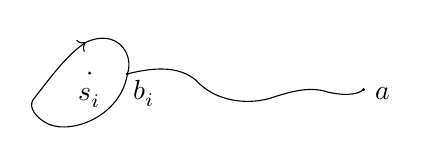
\begin{tikzpicture}[x=1cm,y=1cm,line cap=round,line join=round,baseline=(current bounding box.center)]
\coordinate (b) at (0.48,0.15);
\coordinate (a) at (3.48,-0.05);
\draw[->] (-0.72,-0.18) .. controls (-0.50,0.10) and (-0.30,0.38) .. (-0.05,0.55);
\draw (-0.05,0.55) .. controls (0.33,0.73) and (0.57,0.42) .. (b)
  .. controls (0.40,-0.37) and (-0.20,-0.62) .. (-0.52,-0.49)
  .. controls (-0.68,-0.41) and (-0.78,-0.28) .. (-0.72,-0.18);
\fill (0,0.16) circle (0.6pt);
\node[below] at (0,0.09) {$s_i$};
\fill (b) circle (0.6pt);
\node[below right,inner sep=2pt] at (b) {$b_i$};
\draw (b) .. controls (0.80,0.23) and (1.12,0.26) .. (1.35,0.07)
  .. controls (1.58,-0.19) and (1.98,-0.25) .. (2.29,-0.16)
  .. controls (2.59,-0.06) and (2.81,-0.01) .. (3.02,-0.08)
  .. controls (3.19,-0.12) and (3.38,-0.13) .. (a);
\fill (a) circle (0.6pt);
\node[right,inner sep=4pt] at (3.48,-0.10) {$a$};
\end{tikzpicture}}
et un pt \inserted{\(b_i\)} sur le bord, et une classe d'homotopie de chemins \inserted{(dans \(\deleted{\unsure{X}}\unsure{U|X}-(\mathring\Delta_i-\{s_i\})=V_i\))} de \(a\) vers \(b_i\), et de prendre le groupe \(L_i\) engendré par l'un quelconque des deux lacets correspondants autour de \(s_i\) (qui donnent des \deleted{\unsure{deux}} élts opposés de \(\pi\)).
On voit que l'on trouve ainsi une application surjective de
\[
\operatorname{Isom}_{\Pi_1V_i}(a,b_i)\simeq
\operatorname{Isom}_{\Pi_1U}(a,b_i)
\]
\deleted{vers} sur l'ens des \(L_i\subset\pi\) dans la classe \(\unsure{i|\Pi}\), application \deleted{dont} compatible avec l'action

\scanpage{184}
\mspage{92}

naturelle de \(\pi\) (opérant sur \(\operatorname{Isom}_{\Pi_1U}(a,b_i)\) de la façon évidente par composition, et sur l'ens des \(L_i\) par autom. int.
\deleted{\unsure{Alors}} Ici, le \deleted{choix de} lien avec la description ``abstraite'' toposique s'établit ainsi: le choix de \(b_i\) peut servir de pt \unsure{base|fixe} pour définir un rev. universel de \(\Delta_i\smallsetminus\{s_i\}\overset{\sim}{\hookleftarrow}D_i^*\), d'où un objt \(\rho_!(\widetilde D_i^*(b_i))\), et \deleted{\unsure{cet objt}} les \(L_i\subset\pi\) correspondent \inserted{(d'après la description abstraite)} aux isom de \(\widetilde U_0=\widetilde U(a_i)\) sur \(\unsure{D_i^*(b_i)|\widetilde D_i^*(b_i)}\) modulo composition avec un autom de \(\unsure{D_i^*(b_i)|\widetilde D_i^*(b_i)}\) provenant d'un autom de \(\unsure{D_i^*(b_i)|\widetilde D_i^*(b_i)}\) -- mais les iso \deleted{de} \(\widetilde U(a_i)\xrightarrow{\sim}\rho_!(\widetilde D_i^*(b_i))\) correspondent justement aux classes de chemins de \(a\) vers \(b_i\).

\margin{On revient aux notations \(\pi',U'\) --}
\unsure{Considérons} un objt de \(\Pi_1B_{D_i^{*'}}\), i.e. un couple \((\pi',L_i')\). Soit \(\pi\) le groupe quotient de \(\pi'\) par le ss-groupe invariant de \(\pi'\) \deleted{défini} \inserted{engendré} par \(L_i'\). Je dis \margin{\(\Vert\)} qu'à isom unique près (isom effectif de groupes, pas seulement extérieur !) il ne

\scanpage{185}

dépend pas du choix de l'objt \(\widetilde D_i^*\) de \(\Pi_1B_{D_i'^*}\). En effet, \(\pi=\pi(\widetilde D_i^*)\) dépend fonctoriellement de \(\widetilde D_i^*\), et tt revient à voir que ce foncteur est \uline{constant}, i.e. que l'opération de
\[
\operatorname{Aut}(\widetilde D_i^*)\simeq T\simeq L_i
\quad\text{sur}\quad
\pi=\pi(\widetilde D_i^*)
\]
est triviale. Or soit \(u\in L_i\), \unsure{l'|son} autom de \(\pi\) qu'il définit est défini par l'autom. intérieur \(\operatorname{int}(u)\) par passage au quotient, donc (comme \(u\) devient \(1\) dans \(\pi\)) il est trivial. \unsure{Facile.}

On trouve ainsi un \uline{foncteur}
\[
\begin{array}{c}
\text{Groupes extérieurs à lacets }\pi'\\
\text{de type }g,\nu+1\text{ munis d'une}\\
\text{classe de lacets }i\in I(\pi')
\end{array}
\longrightarrow
\begin{array}{c}
\text{groupes}\\
\text{(réalisés)}\\
\text{à lacets, de}\\
\text{type }g,\nu\deleted{\unsure{+1}}
\end{array}
\]
\[
(\pi',i)\longmapsto\beta(\pi',i)
\qquad
\text{[``bouchage du trou \(i\)'']}
\]
qui s'exprime par un hom de groupes
\[
\operatorname{Aut\,ext}(\pi',i)\longrightarrow\operatorname{Aut}\pi
\tag{\unsure{*|5}}
\]
où \(\pi=\beta(\pi',i)\)
\[
\left(
\begin{array}{l}
\overset{\text{déf}}{=}\text{ ens. des autom cat.}\\
\text{de }\pi'\text{ respectant la structure}\\
\text{à lacets et fixant la classe de}\\
\text{lacets }i
\end{array}
\right)
\]

\scanpage{186}
\mspage{93}

Du point de vue géométrique, ce fait (existence de ce foncteur), ne fait qu'exprimer le fait qu'après ``bouchage du trou'' \(i\), on a un \deleted{pt.} \(U=U'\cup\{s_i\}\) \uline{muni} d'un pt \(s_i\) qu'on peut utiliser comme un \uline{pt base} \inserted{\uuline{canonique}} pour calculer \(\pi_1(U)\).

On peut dire aussi que le choix de \(i\) permet de construire la somme amalgamée partielle (bouchage de trous \inserted{partiel}) \(B_{U^*}\)
\diagram{
\begin{tikzcd}[ampersand replacement=\&]
\& B_{D_i'^*} \arrow[dl] \arrow[dr] \& \\
B_{U'} \arrow[dr] \& \& B_{s_i} \arrow[dl] \\
\& B_{U^*} \&
\end{tikzcd}
}
et \(B_{s_i}\longrightarrow B_{U^*}\) fournit un pt géom. de \(B_{U^*}\) qui permet de décrire un objt canonique de \(\Pi_1B_{U^*}\) (rev universel relatif à ce pt) d'où canoniquement un groupe \(\pi\), qui bien sûr est un groupe à lacets de type \(g,\nu-1\).

\uline{Théorème} Supposons \(g,\nu\) tels que non

\scanpage{187}

seulement les groupes \(\pi'_{\unsure{s}}\) de type \(g,\nu\), mais aussi les groupes \(\pi\) (de type \(g,\nu-1\)) soient anabéliens, i.e.
\[
2g+\unsure{\nu}\deleted{\unsure{+1}}\unsure{\ge|\le}\unsure{4}
\quad
[\text{donc }g\ge2,\ \text{ou }g\unsure{\ge|=}1,\nu\ge2,\ \text{ou }g=0,\nu\ge4].
\]
Alors le foncteur précédent \((\pi',i)\longrightarrow\pi\) est une équivalence de catégories, en d'autres termes (comme il s'agit de groupoïdes \(0\)-connexes)
\[
\operatorname{Aut\,ext}(\pi',i)\longrightarrow\operatorname{Aut}(\pi)
\]
est un \uline{isomorphisme}.

Notons pour ceci \unsure{qu'on a} la suite exacte
\[
1\longrightarrow\pi\longrightarrow\operatorname{Aut}(\pi)
\longrightarrow\operatorname{Aut\,ext}(\pi)\longrightarrow1:
\]
(car \(\operatorname{Centre}\pi=1\) par hyp anabélienne sur \(\pi\)), \unsure{or} on va définir une suite exacte
\[
1\longrightarrow\pi\longrightarrow\operatorname{Aut\,ext}(\pi',i)
\longrightarrow\unsure{\operatorname{Aut\,ext}(\pi)|\operatorname{Aut\,ext}(\pi')}
\longrightarrow1
\]
et un hom. d'extensions de celle-ci

\scanpage{188}
\mspage{\unsure{94|99}}

dans la précédente (qui sera nécessairement un isomorphisme).

OPS \(T=\mathbb Z\), on considère les groupes à lacets \unsure{standart|standard} \(\Pi_{g,\nu+1}\), \(\Pi_{g,\nu}\). Posons
\[
\operatorname{Aut\,ext}_{\mathrm{lac}}(\Pi_{g,\nu})
=\unsure{\mathcal T|\mathfrak T}_{g,\nu}^{\unsure{00|\circ\circ}}
\]
\inserted{induisant \uline{l'identité} sur \(I(\Pi_{g,\nu})\) et sur \(T(\Pi_{g,\nu})\)}
(groupe de Teichmüller d'indice \(g,\nu\)),
on sait que (pour \(2g+\nu\ge3\)) \(\mathcal T_{g,\nu}\) est le groupe fondamental du topos modulaire complexe \inserted{\(M_{g,\nu}\)} des courbes complexes (\deleted{\illegible{1}} \unsure{proj. n.s.}) conn., de genre \(g\), avec un syst de \(\nu\) pts \(s_1-\!s_\nu\) distincts donnés.
\margin{\uline{NB.} le rev. universel de \(M_{g,\nu}\) est contractible, Teichmüller.}
Or le topos modulaire \(M_{g,\nu+1}\) n'est autre que \deleted{l'image} la ``courbe complexe universelle \deleted{\illegible{1}} de genre \(g\) à \(\nu\) trous numérotés'' sur \(M_{g,\nu}\)
[car se donner une courbe \inserted{\(U'\)} de genre \(g\) avec \(\nu+1\) trous \inserted{\(x_1-\!x_{\nu+1}\)} revient au \(\overline{\mathrm m}\) que de s'en donner une \inserted{\(U\)} avec \(\nu\) trous numérotés \(x_1-\!x_\nu\), \uline{plus} un \deleted{trou de} pt de \(U\) \deleted{\unsure{pointé}}), \uline{d'où} une suite exacte d'homotopie
\diagram{
\begin{tikzcd}[ampersand replacement=\&,column sep=small]
\unsure{\pi_2|\Pi_2}(M_{g,\nu},\unsure{\xi})
 \arrow[r] \&
\pi_1(U) \arrow[r] \arrow[d,equal] \&
\pi_1(M_{g,\nu+1}) \arrow[r] \arrow[d,equal] \&
\pi_1(M_{g,\nu}) \arrow[r] \arrow[d,phantom,sloped,"\simeq"] \&
\pi_0(U) \arrow[d,equal] \\
0 \arrow[r] \&
\pi=\Pi_{g,\nu} \arrow[r] \&
\mathcal T^{00}_{g,\nu+1} \arrow[r] \&
\mathcal T^{00}_{g,\nu} \arrow[r] \&
1
\end{tikzcd}
}

\scanpage{189}

d'où \unsure{une} structure d'extension \deleted{annoncée}
\[
1\longrightarrow\Pi_{g,\nu}
\longrightarrow\mathcal T^{00}_{g,\nu+1}
\longrightarrow\mathcal T^{00}_{g,\unsure{\nu}}
\longrightarrow1
\]
qui est (à passage à un sous-groupe d'indice ``\(2\nu!\) près) cette structure d'extension annoncée. \unsure{\&} les vérifications de \uline{compatibilité} sont laissées \ldots.

On a donc un foncteur quasi inverse (défini à isom unique près)
\[
\begin{array}{c}
\text{groupes à lacets}\\
\text{de type }g,\nu\\
(2g+\nu\ge3)
\end{array}
\longrightarrow
\begin{array}{c}
\text{groupes \uline{extérieurs} à}\\
\text{lacets de type }(g,\nu+1),\\
\text{avec une ``classe de}\\
\text{lacets'' distinguée}\\
\text{(couples }(\pi',i\in I(\pi'))\text{)}
\end{array}
\]

\deleted{\unsure{Or}} \unsure{Au} niveau toposique, quand on a un système \(B_{D^*}\longrightarrow B_U\) \inserted{de type \(g,\nu\) \((2g+\nu\ge3)\)}, et un ``pt'' de \(B_U\) i.e un \(\widetilde U\in\operatorname{Ob}\Pi_1B_U\), alors on peut de façon canonique trouver un \(B_{D_i^*}\) (\unsure{\(T\)-gr. poïde} \inserted{connexe}, où \(T\) est le module d'orientation), et un système
\[
B_{D^*}\amalg B_{D_i^*}\longrightarrow B_{U'},
\]
de type \(g,\nu+1\),

\scanpage{190}
\mspage{95}

de façon que \((B_{D^*},B_U,\widetilde U)\) \unsure{s'en déduise} par l'opération de ``bouchage du trou \(D_i^*\)''.

Ces constructions sont si fonctorielles, \margin{\unsure{\(\wedge\)}} qu'elles commutent aux actions de groupes \(\Gamma\). Si un groupe \(\Gamma\) opère sur un groupe à lacets \(\pi_{\deleted{\unsure{g,\nu}}}\) de type \(g,\nu\), (pas seulement extérieurement), alors on en déduit une opération \uline{extérieure} de \(\Gamma\) sur un \(\pi'\) à lacets de type \(g,\nu+1\), qui fixe une classe de lacets privilégiée \(i\in I\).

Mais alors, dans l'extension correspondante
\[
1\longrightarrow\pi'\longrightarrow E'\longrightarrow\Gamma\longrightarrow1,
\]
Choisissons un \(L_i'\subset\pi'\) et soit \(\unsure{\mathcal E_i'|E_i'}\) le normalisateur de \(L_i\) dans \(\unsure{\mathcal E'|E'}\) -- on trouve
\[
1\longrightarrow
\underset{\simeq T}{L_i'}
\longrightarrow\unsure{\mathcal E_i'|E_i'}
\longrightarrow\Gamma\longrightarrow1
\]
\scanpage{191}
% l. 01
( ceci \unsure{marche} \unsure{s.s} hyp. de finitude sur
% l. 02
$\Gamma$, le cas universel étant celui où $\Gamma$
% l. 03
est le \unsure{grpe} de Teichmüller de $\pi'$ \unsure{fixt} $i$
% l. 04
i.e. $\operatorname{Autext}_{\mathrm{lac}}(\pi';i)\simeq\operatorname{Aut}_{\mathrm{lac}}(\pi)$ ). Je
% l. 05
dis que si $\Gamma$ opère \uline{fidèlt} \uline{sur $\pi$}
% l. 06
i.e. si son opération extérieure \uline{sur}
% l. 07
\uline{$\pi'$} est fidèle, et si $\Gamma$ est \uline{fini},
% l. 08
Alors $\Gamma$ est nécessairement cyclique \inserted{(cas $\Gamma=\Gamma^0$)}
% l. 09
ou dihédral ($\Gamma\ne\Gamma^0$), et que si de
% l. 10
plus $\Gamma=\Gamma^0$, alors \deleted{\unsure{$\mathcal E_i'$ est $\simeq$}} \inserted{\unsure{$\mathcal E_i\simeq\mathbb Z$|$\mathcal E_i'\simeq\mathbb Z$} i.e.} $\exists!$ isom
% l. 11
\unsure{$T\xrightarrow{\sim}\mathcal E_i$|$T\xrightarrow{\sim}\mathcal E_i'$} tel que \unsure{$T\xrightarrow{k_i'}\mathcal E_i'$} s'identifie à
% l. 12
$n\operatorname{id}_T$ (de sorte qu'on trouve \unsure{$\Gamma\simeq\mathcal E_i'/n\mathcal E_i'$}
% l. 13
$\simeq T\otimes_{\mathbb Z}\mathbb Z/n\mathbb Z$, si $n=\operatorname{card}\Gamma$ ...

% l. 14
Changeant de notations, ceci revient au
% l. 15
\uline{Th}\textsuperscript{\unsure{m}} Soit $\Gamma$ un groupe fini opérant
% l. 16
fidèlt sur un groupe \uline{\unsure{extérieur|extérieurem\textsuperscript{t}}} à
% l. 17
lacets $\pi$ \inserted{de type \deleted{\illegible{1}} $(g,\nu+1)$ ($\nu\geq0$)}, en laissant fixe un $i\in I(\pi)$,
% l. 18
Alors $\Gamma$ est cyclique (si $\Gamma=\Gamma^0$) ou
% l. 19
dihédral (si $\Gamma\ne\Gamma^0$), et dans l'extension
% marge, en bas à gauche
\margin{\unsure{au} $\overline{\mathrm m}$ il y a \uline{équivalence}, si dans le th, on suppose le type $(g,\nu)$ anabélien --- sinon le th. est un peu plus général}
\mspage{190}


\scanpage{192}
\mspage{96}
% l. 01
correspondant \deleted{\illegible{2}} \unsure{$\mathcal E$} de $\Gamma$ par $\pi$,
% l. 02
Si \unsure{$\mathcal E_i$} est le normalisateur de un $L_i$ dans
% l. 03
\unsure{$\mathcal E$} [ \inserted{de sorte qu'on a} \deleted{une} \unsure{$\mathcal E_i\to\Gamma$} épi i.e. une suite exacte
% l. 04
\unsure{$1\to L_i\to\mathcal E_i\to\Gamma\to1$} ]. l'image inverse \unsure{$\mathcal E_i^0$} de
% l. 05
$\Gamma^0$ est $\simeq\mathbb Z$ donc (si $n=\operatorname{card}\Gamma^0$)\inserted{\unsure{$=[\mathcal E_i^0:L_i]$}}
% l. 06
\deleted{\unsure{$n\operatorname{id}$}} $x\to x^n$ est un iso. \deleted{et} \unsure{$\mathcal E_i^0\simeq L_i$}, qui
% l. 07
compte tenu de $k_i$ donne un
% l. 08
isom \unsure{$\mathcal E_i^0\simeq T$}, dont le composé avec
% l. 09
\deleted{\unsure{$\mathcal E_i$}} \unsure{$T\xrightarrow[\sim]{k_i}L_i\subset\mathcal E_i^0$} est $n\operatorname{id}_T$, de sorte
% l. 10
qu'on a un iso. can
% l. 11
\[\unsure{\Gamma^0\simeq\mathcal E_i^0/L_i\simeq T/nT}\]
% l. 12
(évidemment indépendant du choix de $L_i$ ...)

% l. 13
\uline{Démonstration}. Considérons l'extension
% l. 14
\unsure{$\mathcal E_i^0$} de $\Gamma^0$ par $L_i\simeq T$ ($\overset{\text{\unsure{non can}}}{\simeq}\mathbb Z$),
% l. 15
comme \unsure{$\mathcal E_i^0$|$\Gamma^0$} opère trivialem\textsuperscript{t} sur $T$ \inserted{sans torsion}, cette
% l. 16
extension (par la suite exacte de coh.
% l. 17
associée à $0\to T\to T\otimes_{\mathbb Z}\mathbb Q\to T\otimes_{\mathbb Z}\mathbb Q/\mathbb Z\to0$)
% l. 18
est canoniquem\textsuperscript{t} isomorphe à \deleted{\unsure{une}} l'extension
% l. 19
définie par un hom $\Gamma^0\to T_n=T/nT$,
% l. 20
comme image inverse de l'extension
% l. 21
$0\to T\xrightarrow{n}T\to T_n\to0$ de $T_n$ par $T$. Je dis que
\mspage{191}


\scanpage{193}
% l. 01
cet hom. est un iso (d'où \unsure{résulteraient|résulteront}
% l. 02
les autres assertions), ou ce qui revient
% l. 03
au $\overline{\mathrm m}$ puisque $\Gamma^0$ et $T_n$ sont tous
% l. 04
deux d'ordre $n$, que c'est mono.
% l. 05
Remplaçant $\Gamma^0$ par le noyau de $\Gamma^0\to\mathbb Z/n\mathbb Z$,
% l. 06
OPS que l'hom. \inserted{en question} est nul, et il faut
% l. 07
prouver que cela implique que l'action
% l. 08
de $\Gamma^0$ est triviale (ce qui, puisque par hyp.
% l. 09
l'action de $\Gamma$ est fidèle, implique $\Gamma^0=\{1\}$,
% l. 10
OK.) Donc \unsure{th} est ramené au

% l. 11
\uline{lemme fondamental}. Tout automorphisme \inserted{direct}
% l. 12
extérieur $u$ d'ordre fini \inserted{\unsure{$n$}} d'un groupe à
% l. 13
lacets $\pi$, qui fixe une classe de lacets
% l. 14
$i$ et est tel que l'extension de $\mathbb Z/n\mathbb Z$
% l. 15
par $L_i\in i$ définie par $u$ soit triviale,
% l. 16
est trivial.

% l. 17
L'hypothèse signifie que $u$ se remonte
% l. 18
en un autom $u_0$ de $\pi$, qui
% l. 19
normalise $L_i$, et qui soit aussi d'ordre \unsure{$n$},
% l. 20
(ou d'ordre fini, cela revient au \unsure{$\overline{\mathrm m}$|$\Rightarrow$} compte tenu
% l. 21
que \deleted{\unsure{les élts de}} $T$ est sans élts d'ordre fini)
\mspage{192}


\scanpage{194}
\mspage{97}
% l. 01
alors $u_0$ est trivial, i.e. cela équivaut au
% l. 02
\uline{Corollaire}. Tout autom \inserted{direct} d'ordre fini \inserted{$u_0$} d'
% l. 03
un groupe à lacets $\pi$, \inserted{qui soit direct et} qui normalise
% l. 04
un sous-groupe à lacets $L_i$ (i.e. qui
% l. 05
centralise $L_i$), est réduit à l'identité.
% marge supérieure gauche
\margin{Dans le lemme ou son \unsure{coroll.}}
\margin{\uline{NB} (le cas $g=0$, $\nu+1=1$ ou $\nu+1=2$ est trivial, le cas $\nu+1=3$ ($(g,\nu)=(0,2)$ abélien!) n'est pas trivial \unsure{par contre}, ni le cas $g=1$, $\nu+1=1$ i.e. $(g,\nu)=(1,0)$ abélien. Pourtant le résultat doit être valable aussi dans \unsure{ce|ces} cas.)}

% l. 06
Pour le démontrer, on est ramené \inserted{aussitôt} au
% l. 07
cas où $u_0$ est \deleted{d'ordre premier $p$} \inserted{tel que $u_0^p=\operatorname{id}$, où}
% l. 08
$p$ est un \unsure{nb} premier --- i.e. $u_0$ corres-
% l. 09
pond à une opération au sens strict
% l. 10
(pas seulem\textsuperscript{t} extérieure) de $\mathbb Z/p\mathbb Z$ \deleted{\unsure{par}} \unsure{à autom}
% l. 11
de $\pi$. Mais (que l'on puisse ou non
% l. 12
trouver un tel $p$) considérons le cas où
% l. 13
on sait que l'opération \uline{extérieure} de
% l. 14
$\Gamma=\mathbb Z/n\mathbb Z$ [$n=$ ordre de $u$] sur $\pi$ se réalise
% l. 15
géométriquem\textsuperscript{t}, par une opération (fidèle)
% l. 16
de $\Gamma=\mathbb Z/n\mathbb Z$ sur une $U$ de type $(g,\nu+1)$.
% l. 17
\deleted{\unsure{classes de $\pi$-conjugaison}, \illegible{1}}
% marge inférieure gauche
\margin{$U=X\setminus S$, $S\simeq I$, $X$ comp. de genre $g$ \unsure{la pointe|la partie} $s_i$ de $S$ correspondant à un pt fixe de $\Gamma$ op. sur $U$.}

% l. 18
\deleted{On sait que les (\unsure{relèvements}) des auts
% l. 19
extérieurs en \deleted{\unsure{des autom}} \inserted{une vraie opération},
% l. 20
correspondent aux pts fixes \illegible{1} de $\Gamma$
% l. 21
dans $U$; \deleted{et l'extension de} \inserted{soit $a$ le pt fixe de $\Gamma$}
% l. 22
correspondant à l'opération donnée, \unsure{de}
% l. 23
sorte qu'on a \deleted{\unsure{un}} iso. can. \unsure{compatible avec $\Gamma$}
% l. 24
$\pi=\pi_1(U,a)$.}
\mspage{193}


\scanpage{195}
% l. 01
On exprime l'hyp. de l'opération \inserted{\unsure{``véritable''}} de $\Gamma$ sur
% l. 02
$\pi$, \deleted{\illegible{1}} \unsure{centralis.} un $L_i$, en disant que
% l. 03
l'opération extérieure donne une extension
% l. 04
de $\Gamma$ par $L_i\simeq T$ triviale. Mais on sait
% l. 05
par ailleurs dans le cas géom. \inserted{et op. fidèle} qu'elle
% l. 06
n'est \uline{pas} triviale !

% l. 07
Il suffirait donc, \deleted{\illegible{1}} pour prouver le
% l. 08
lemme fondamental, de savoir que tte
% l. 09
action extérieure \inserted{[fidèle]} d'un groupe cyclique
% l. 10
sur un groupe à lacets de type \unsure{$(g,\nu+1)$}
% l. 11
est réalisable, et il suffit $\overline{\mathrm m}$ de le savoir
% l. 12
pour un groupe cyclique d'ordre
% l. 13
premier. \inserted{\unsure{est}} \unsure{Or} sauf erreur ce résultat
% l. 14
est \unsure{bien} connu ($\overline{\mathrm m}$ pour les groupes \unsure{ré-}
% l. 15
solubles ...). --- de sorte que le lemme fon-
% l. 16
damental semble démontré. J'ai seulement
% l. 17
un doute s'il est démontré dans le
% l. 18
cas général d'un $(g,\nu)$, \inserted{\deleted{\illegible{1} $g\geq2$}} ou seulement
% l. 19
pour \inserted{$g\geq2$,} $\nu=0$. Mais \deleted{à vrai dire, \illegible{2}, \inserted{cela suffit}}
% l. 20
\deleted{\illegible{2} \inserted{pour $g\geq2$}}
% marge inférieure gauche
\margin{comme th. \unsure{d'exist.} \unsure{de pts} fixes d'un groupe \illegible{1} \unsure{opér.} \unsure{de} Teichmüller}

% l. 21
\deleted{\uline{Lemme} Soit \illegible{1} une opération extérieure}
\mspage{194}


\scanpage{196}
\mspage{98}
% l. 01
\deleted{d'un groupe fini $\Gamma$ sur un \illegible{1}} s'il en
% l. 02
est bien ainsi, je pense que (pour $g\geq2$ tout
% l. 03
au moins) on s'en tire par dévissage
% l. 04
pour le cas $\nu$ quelconque --- et le cas $g=0,1$
% l. 05
demanderait \inserted{\unsure{aussi}} un traitement à part.
% l. 06
Je reviendrai là-dessus par la suite, et
% l. 07
préfère pour l'instant admettre le ``lemme
% l. 08
fondamental'', et examiner des conséquences
% l. 09
et corollaires de celui-ci.

% l. 10
Pour une action extérieure \inserted{fidèle} d'un $\Gamma$ fini
% l. 11
sur un groupe à lacets \uline{anabélien} $\pi$, \unsure{on}
% l. 12
\deleted{\unsure{a établi}} correspondant à une extension \unsure{$\mathcal E$} de $\Gamma$ par $\pi$,
% l. 13
on a donc établi a) que les scindages
% l. 14
partiels de celle-ci ne peuvent se faire
% l. 15
que sur des ss-groupes \deleted{\unsure{cycliques}} $\Gamma'$ de $\Gamma$
% l. 16
tels que $\Gamma'{}^0$ \unsure{soit} cyclique, et $\Gamma'$ dihédral
% l. 17
si $\Gamma'\ne\Gamma'{}^0$, et que b) pour tte classe
% l. 18
de \illegible{2} de tels scindages partiels
% l. 19
\unsure{sur} $\Gamma'\subset\Gamma^0$, on a un iso. can.
% l. 20
correspondant $\Gamma'\simeq T_n$ ($=T/nT$), où $n=\operatorname{card}\Gamma'$.
% marge inférieure gauche
\margin{i.e. on a établi l'existence d'une \unsure{applic.} can. \illegible{1} des \unsure{éléments} d'ordre fini de $\operatorname{Aut}_{\mathrm{lac}}(\pi)$ dans \unsure{$T\otimes\mathbb Q/T$}, satisfaisant \unsure{les} conditions \unsure{examinées} précédemment}

% l. 21
Ce sont là des résultats qu'on avait
\mspage{195}


\scanpage{197}
% l. 01
précédemment obtenus pour le cas d'une
% l. 02
opération \uline{réalisable}. [Il n'y avait pas lieu
% l. 03
d'ailleurs de se borner au cas anabélien,
% l. 04
du moment qu'on \unsure{suppose} $\pi\ne0$ \inserted{(cas essentiellement vide!)},
% l. 05
ce qui inclut les cas \inserted{abéliens} $g=0$, $\nu=2$ et
% l. 06
$g=1$, $\nu=0$, pour lesquels un traitement
% l. 07
direct est possible, et a déjà été donné
% l. 08
essentiellement, les cas-là \deleted{\unsure{étant} réalisables,} \inserted{\unsure{où|si l'on}}
% l. 09
part d'une \uline{extension} (pas d'une action
% l. 10
``extérieure'' i.e. ici d'une action tout court
% l. 11
de $\Gamma$ sur $\pi\simeq\mathbb Z$ ou $\mathbb Z^2$), \unsure{étant} tjrs \unsure{réalisables}.
% l. 12
(\uline{NB} \deleted{\unsure{l'hyp.}} \inserted{Dans ce} cas, l'hypothèse d'une
% l. 13
action fidèle est remplacée par celle que
% l. 14
l'extension n'est \deleted{\unsure{pas scindable}} \inserted{une extension \uline{produit}} \unsure{sur|sous} aucun
% l. 15
sous-groupe $\Gamma'\subset\Gamma^0$ avec $\Gamma'\ne1$ ....).

% l. 16
Il reste cependant d'autres résultats du
% l. 17
cas réalisable, qu'il faudrait examiner
% l. 18
dans le cas général :

% l. 19
c) Si $\Gamma$ est un sous-groupe \deleted{\unsure{discret}} fini
% l. 20
de $\operatorname{Aut}_{\mathrm{lac}}(\pi)$ i.e. un grpe fini opérant \uline{\unsure{fidèlt}}
% l. 21
sur $\pi$, a-t-on $\pi^\Gamma=\{1\}$ ?
% marge inférieure gauche
\margin{OPS $\Gamma=\Gamma^0$ donc $\Gamma$ engendré par un autom. direct \unsure{$u$} ou $\Gamma$ engendré par un \unsure{anti-autom.} d'ordre 2}
\mspage{196}


\scanpage{198}
\mspage{99}
% l. 01
d) \unsure{Si} $\Gamma',\Gamma''$ sont des ss-groupes finis de \unsure{$\mathcal E$}
% l. 02
\unsure{(ext.} du groupe fini $\Gamma$ par $\pi$, correspondant
% l. 03
à une opération \deleted{\unsure{respect}} extérieure \inserted{(respectant l'orientation)} fidèle), \deleted{\illegible{1}}
% l. 04
tels que $\Gamma'\cap\Gamma''\ne(1)$, alors \deleted{l'un des
% l. 05
deux contient-il l'autre} ?
\inserted{$\Gamma'$ et $\Gamma''$ sont-ils contenus dans le $\pi$-conjugué d'un ss-gpe fini $\Gamma'''$ de \unsure{$\mathcal E$} [i.e. tt sous-\unsure{groupe} section $\ne1$ est contenu dans un unique sous-groupe section \unsure{maximal}, mod. $\pi$-conjugaison}
% marge supérieure gauche
\margin{\uuline{NB} Deviendrait faux en \deleted{\illegible{1}} \unsure{plaçant} dans le groupe $\operatorname{Aut}_{\mathrm{lac}}(\pi)$ \illegible{2} \unsure{l'un en ss-gr.} \illegible{2} \unsure{l'un des deux ss.} \unsure{contenu dans} \illegible{4}}

% l. 06
e) Pour tt \unsure{ss-gpe}, \illegible{2} \deleted{\illegible{1}} $\Gamma'$ de $\Gamma$,
% l. 07
\unsure{l'ens.} des classes \deleted{\unsure{d'extensions}} $\pi$-conjugaison
% l. 08
de relèvements de $\Gamma'$ en \unsure{$\mathcal E$} est-il fini ?
% l. 09
[OPS $\Gamma'=\Gamma$, et $\Gamma$ cyclique (si $\Gamma=\Gamma^0$) ou dihédral
% l. 10
(sinon)]
% l. 11
\inserted{Dans le cas \unsure{c)|e)}, OPS $\Gamma$ cyclique d'ordre premier, et
% l. 12
c'est OK s'il est acquis qu'une \unsure{op. extérieure} \illegible{3}
% l. 13
\unsure{que} \illegible{4} \unsure{$\pi_{g,\nu}$} \deleted{\illegible{3}} \unsure{d).}} \deleted{En appliquant}
% marge gauche, au milieu
\margin{\unsure{De} $\overline{\mathrm m}$ e) est établi si \unsure{on} admet que les op. ext. de \unsure{groupes cycliques} \unsure{sur un} $\pi\simeq\pi_{g,\nu}$ sont réalisables}

% l. 14
\deleted{Ex. examinons \illegible{2}
% l. 15
la \unsure{joncture|jonction} ``forage de trous'', $\Gamma'$ et $\Gamma''$
% l. 16
opérant extérieurement sur un $(\pi';i)$
% l. 17
$i\in I(\pi')$ --- leur action sur $\pi$ est
% l. 18
déduite de celle sur $(\pi',i)$ en ``bouchant
% l. 19
le trou $i$''. Ceci dit, $\Gamma'$ et $\Gamma''$ sont identifiés
% l. 20
aux ss-groupes finis de $\operatorname{Autext}_{\mathrm{lac}}(\pi';i)$
% l. 21
On a mieux :
% l. 22
\unsure{$\Gamma=\Gamma'\cap\Gamma''\ne(1)$}}

% Un trait oblique part du coin inférieur gauche du cadre et traverse « Soit » et « et considérons » ; sa portée comme biffure est incertaine.
\unsure{\deleted{
% l. 23
\uline{Théorème}. Soit $\Gamma_0$ \deleted{\illegible{1}} un sous-groupe fini de
% l. 24
$A=\operatorname{Aut}_{\mathrm{lac}}(\pi)^0$, \inserted{$\Gamma_0\ne1$}, \deleted{\illegible{1} et considérons} Alors le normalis. $N$
% l. 25
de \unsure{$\Gamma$|$\Gamma_0$} dans $A$ est égal à son centralisateur \unsure{$Z$|$\mathcal Z$}
}}
\margin{\uuline{Ultra fort!} \unsure{Si $g=0$}}
\mspage{197}


\scanpage{199}
% Un trait oblique traverse le corps de cette page ; sa portée comme biffure est incertaine.
\unsure{\deleted{
% l. 01
et l'ensemble des élts d'ordre fini
% l. 02
de \unsure{$Z$|$\mathcal Z$} est un groupe cyclique \inserted{\unsure{$F$|$\Gamma$}}, \deleted{contenu
% l. 03
dans} qui est aussi le plus grand sous-
% l. 04
groupe fini de $A$ contenant $\Gamma_0$, et est
% l. 05
contenu dans le centre de \unsure{$Z$|$\mathcal Z$}.

% l. 06
Le fait que le normalisateur $N$
% l. 07
centralise $\Gamma_0$ provient du fait que l'on
% l. 08
a un iso can. (compatible aux \unsure{transports}
% l. 09
de \unsure{structures})
% l. 10
\[\Gamma_0\xrightarrow{\sim}T_{n_0}\qquad(\text{si }n_0=\operatorname{card}\Gamma_0)\]
% l. 11
(NB si $g\in\operatorname{Aut}_{\mathrm{lac}}(\pi)$ renversant l'orientation,
% l. 12
et \unsure{normalise|centralise} $\Gamma_0$, alors \deleted{\unsure{$g$}} $(\operatorname{int}g)$ induit
% l. 13
la symétrie $\sigma\to\sigma^{-1}$ sur $\Gamma_0$, par le $\overline{\mathrm m}$
% l. 14
argument) \deleted{\illegible{1}} Notons que si
% l. 15
$u$ est un élt d'ordre fini de \unsure{$Z$|$\mathcal Z$}, de
% l. 16
sorte que $\Gamma_0,u$ engendrent un ss-grpe
% l. 17
comm. fini de \unsure{$Z$|$\mathcal Z$}, \deleted{on voit que} \inserted{comme on sait}
% l. 18
qu'un ss-groupe fini de $A$ est cyclique,
% l. 19
il s'ensuit que $u$ est contenu dans
% l. 20
un sous-groupe cyclique de \unsure{$Z$|$\mathcal Z$} \unsure{cont\textsuperscript{t}} $\Gamma_0$,
% l. 21
\deleted{\unsure{donc}} soit $\Gamma'$. choisissons maintenant
% l. 22
une réalisation géom. de l'action \inserted{ext.} de
% l. 23
$\Gamma_0$ sur \deleted{\illegible{1}} $\pi$, soit $(X,S)$ avec $U=X-S$ ;
}}
\mspage{198}


\scanpage{200}
\mspage{100}
% Un long trait oblique traverse le texte ; sa portée comme biffure est incertaine.
\unsure{\deleted{
% l. 01
on sait que le relèvement de l'action
% l. 02
extérieure de $\Gamma_0$ en une action est
% l. 03
décrit par un unique pt $a\in U$.
% l. 04
\deleted{Soit} Je dis que $\Gamma'$ \deleted{est réalisable} (ou son
% l. 05
action \deleted{extérieure} sur $\pi\simeq\pi_1(U,a)$) est réalisable
% l. 06
de \uuline{façon unique} par une action de $\Gamma'$
\margin{\uuline{pas vrai!}}
\inserted{et induisant l'action déjà donnée de \unsure{$\Gamma$|$\Gamma_0$}}
% l. 07
sur $(X,S)$), fixant $a$, le fait qu'il
% l. 08
soit \inserted{bien} réalisable ainsi provient du fait
% l. 09
(que nous admettons) que tte action
% l. 10
extérieure d'un groupe cyclique \inserted{(ici $\Gamma'$)} sur un
% l. 11
groupe à lacets \inserted{$\pi$} de type $(g,\nu)$ est réalisable,
% l. 12
et de l'unicité d'une telle réalisation
% l. 13
(dans le cas de $\Gamma_0$). Pour l'\uline{unicité},
% l. 14
cela \deleted{\illegible{1}} revient au

% l. 15
\uline{Lemme}. Soit $u_0$ un autom d'ordre fini $n_0\ne1$
% l. 16
d'une surface \inserted{orientable} \deleted{\unsure{supposée} $X^{u_0}\ne\emptyset$.} \inserted{$U=X-S$, $X$ (compacte, \deleted{\illegible{1}}, et} laissant fixe \inserted{un pt $a\in U$} \illegible{1}
% l. 17
soit $d\in\mathbb N^*$, (S'il existe un automorphisme \unsure{$u$} de
% l. 18
\deleted{\illegible{1}} \inserted{$(X,S)$} tel que $u^d=u_0$, \inserted{$u(a)=a$}, alors $u$ est uniquement
\margin{\uline{faux!}}
% l. 19
déterminé par son \deleted{\unsure{classe d'}} action sur $\pi_1(U,a)$;
% l. 20
et en tout état de cause le groupe cyclique
% l. 21
d'autom. de $(X,S)$ engendré par $u$ est \unsure{uniquem\textsuperscript{t}}
% l. 22
\inserted{déterminé (il est d'ordre $nd$).}
}}
\mspage{199}
\scanpage{201}
\uline{Démonstration.} \deleted{Fixons une structure
\deleted{\unsure{conforme}} \inserted{\deleted{\illegible{1}}} \inserted{complexe,}
sur $X$, \unsure{invariante} par}

Démontrons d). \deleted{Soit $\Gamma_0 =$} Nous identifions
$\Gamma',\Gamma''$ à des ss-groupes de $\Gamma$, et posons $\Gamma_0=\Gamma'\cap\Gamma''$.
Soit \unsure{$\mathcal E^!$} le ss-groupe de $\mathcal E$ formé des $g\in\mathcal E$
tels que $\operatorname{int}(g).\Gamma_0$ soit $\pi$-conjugué de $\Gamma_0$
et dont l'image dans $\Gamma$ \deleted{\illegible{1}} centralise $\Gamma_0$.
\deleted{\illegible{1}} On a $\mathcal E^!\supset\pi$, et $\mathcal E^!$ est donc l'image
inverse d'un sous-groupe $\Gamma^!$ de $\Gamma$, qui
centralise $\Gamma_0$ \deleted{\illegible{1}}, et qui contient $\Gamma'$ et $\Gamma''$
(car $\mathcal E^!$ contient le centralisateur de $\Gamma_0$ dans $\mathcal E$,
donc $\Gamma'$ et $\Gamma''$). Quitte à remplacer
$\Gamma$ par $\Gamma^!$, $\mathcal E$ par $\mathcal E^!$, OPS $\mathcal E=\mathcal E^!$, $\Gamma=\Gamma^!$ i.e.
que $\Gamma_0\subset\mathrm{Centre}$ de $\Gamma$, et que $\Gamma_0\hookrightarrow\mathcal E$
\unsure{invariant} mod $\pi$-conjugaison par $\Gamma$.

\deleted{Après quoi choisissons une réalisation top.
$(X,S,a)$ de l'opération \deleted{ext.} de $\Gamma_0$ sur $\pi$,
où $a\in U=X-S$ -- donc $\pi\simeq\pi_1(U,a)$. D'après
le résultat (\unsure{b}) d'existence et d'unicité
des réalisations dans le cas cyclique, cela
est possible, et de plus on peut faire}

\scanpage{202}
\mspage{101}
\deleted{opérer $\Gamma'$ sur \unsure{$(X,S,a)$} (i.e. sur $(U,a)$) de façon
compatible avec son action sur $\pi_1(U,a)=\pi$, de
façon à prolonger l'action de \unsure{$\Gamma_0$|$\Gamma$} --
et de \unsure{$\overline{\mathrm m}$|$=$} pour $\Gamma''$. Mais il n'est pas clair
à priori
que les deux actions \deleted{\unsure{puissent}} soient compatibles
en le sens préc. \deleted{\unsure{du ss-groupe engendré}}
\inserted{que le \unsure{ss-groupe engendré}}
\deleted{\unsure{par} $\Gamma',\Gamma''$} $\subset\operatorname{Aut\,top}(U)$ soit aussi fini.}

\deleted{Considérons maintenant $X'=X/\Gamma_0$, $S'=S/\Gamma_0$,
et l'image $a'$ de $a$ dans $X'$ -- donc $a'\in U'=X'-S'$.
Alors \unsure{$\Gamma/\Gamma_0$|$\Gamma'/\Gamma_0$} opère \unsure{isotypiquement|isotopiquement} sur $(X',S',b)$}

\deleted{Utilisons $\pi^{\Gamma_0}=(1)$, on trouve que}

On va construire une section de $\mathcal E$
sur $\Gamma$ \unsure{tt} entier, ainsi. Soit $\widetilde\Gamma\subset\mathcal E$
le centralisateur de $\Gamma_0$ dans $\mathcal E$, \unsure{on a|$\Rightarrow$}
\deleted{$\gamma\in\Gamma$, $g\in\mathcal E$ au-dessus de $\gamma$, considérons}
$\widetilde\Gamma\cap\pi=(1)$ (car cela signifie $\pi^{\Gamma_0}=(1)$)
\deleted{$\operatorname{int}(g).\Gamma_0$, $\exists!\ \alpha\in$}
\inserted{donc}
\deleted{je dis que} $\widetilde\Gamma\longrightarrow\Gamma$ injectif, je dis
qu'il est surjectif. En effet, soit
$\gamma\in\Gamma$, $g\in\mathcal E$ au dessus de $\gamma$, par hyp
\inserted{sur $\Gamma$}
$\exists\ \alpha\in\pi$ tel que $\operatorname{int}(g).\Gamma_0=\operatorname{int}(\alpha).\Gamma_0$
i.e. OPS $\operatorname{int}(g)\Gamma_0=\Gamma_0$, \deleted{\unsure{donc}} i.e. $g$ normalise
$\Gamma_0$, mais comme $\Gamma_0$ est central dans $\Gamma$
cela signifie que $g$ centralise $\Gamma_0$ i.e. $g\in\widetilde\Gamma$.

\scanpage{203}
Ainsi $\widetilde\Gamma$ \inserted{$\simeq\Gamma$} \unsure{est} un sous-groupe \uline{fini} de $\operatorname{Aut}(\pi)$,
\deleted{donc cyclique} contenant $\Gamma'$ et $\Gamma''$, cqfd.% a dashed line runs under the deleted words (possible restoration mark); unresolved

\uline{NB} Si on n'avait pas au début supposé
$\Gamma$ fini, il serait vrai encore que $\Gamma',\Gamma''$
engendrent un ss-groupe $\widetilde\Gamma$ \inserted{$\subset\operatorname{Aut}(\pi)$} tel que
$\widetilde\Gamma\cap\pi=(1)$, mais cela nous fait une
belle jambe \deleted{-- \unsure{on peut en trouver},
p.ex. isom. à \unsure{$\operatorname{Autext}(\pi,i)$} tout entier,
(pour un \unsure{$i\in I(\pi)$} choisi: prendre le
\deleted{\illegible{2}}
centralisateur de \unsure{$i$} dans \illegible{2} $\operatorname{Aut}(\pi)$)}

\scanpage{204}
\mspage{102}
19. Tour de Teichmüller.

Soit \inserted{$g\in\mathbb N$, et} $X_g$ une surface compacte orientable de
genre $g$, \deleted{\unsure{l'ensemble des orientations},}
\unsure{$[$|$]$} $(a_{g,i})_{i\in\mathbb N^*}=(a_{g,1},a_{g,2},\ldots)$ \unsure{$]$|$[$}
une suite de
pts distincts de $X_g$. On pose pour \unsure{$\forall\nu\in\mathbb N$}
\[
(1)\qquad S_{g,\nu}=\{\unsure{x_{g,i}|a_{g,i}}\mid 0\leq i\leq\nu-1\}
\qquad\text{donc }\nu=\operatorname{card}S_{g,\nu}
\]
\[
(2)\qquad U_{g,\nu}=X_g-S_{g,\nu}.
\]
\margin{NB on \unsure{a} $a_{g,\nu}\in U_{g,\nu}$}
On a donc $S_{g,0}=\varnothing$, $U_{g,0}=X_g$; Les $S_{g,\nu}$ forment
une suite \inserted{str.} croissante de parties finies de $X_g$,
les $U_{g,\nu}$ une suite str. décroissante d'ouverts
de $X_g$. On prendra par la suite $U_{g,\nu}$ comme
la surface (orientée, ou orientable) type, de
type $(g,\nu)$.

Soit
\[
(3)\qquad A_g=\operatorname{Aut}(X_g)
\]
le groupe des autom. de $X_g$, muni de la
top. de la conv. uniforme de $u$ et de son
inverse. On pose
\[
(4)\qquad A_{g,\nu}=\{u\in A_g\mid u(S_{g,\nu})=S_{g,\nu}\}\subset A_g
\]
ainsi $A_{g,\nu}$ est un sous-groupe de $A_g$. On
a un isomorphisme canonique $u\mapsto u|U_{g,\nu}$
\[
A_{g,\nu}\xrightarrow{\sim}\operatorname{Aut}(U_{g,\nu}).\qquad(5)
\]
\margin{\uline{NB} C'est \inserted{\unsure{ss doute|sans doute}} \unsure{un isom.}
topologiques, quand $A_{g,\nu}$ est
muni de la top. induite par $A_g$,
et $\operatorname{Aut}(U_{g,\nu})$ de la top. habituelle de la conv.
\unsure{comp.} \illegible{1} de $u$ et son inverse.}
\deleted{\unsure{Soit}} On a \deleted{\unsure{un}} homomorphisme can. surjectif
\[
(6)\qquad A_{g,\nu}\longrightarrow\operatorname{Aut}(S_{g,\nu})
\bigl(\overset{\text{(can)}}{\simeq}\unsure{\mathfrak S_\nu}\bigr),
\]

\scanpage{205}
dont le noyau est noté par $A_{g,\nu}^!$
\[
(7)\qquad A_{g,\nu}^!=\{u\in A_g\mid u(a_{g,i})=a_{g,i},\ \forall i\in[0,\ldots,\nu-1]\}
\]
d'où suite exacte
\[
(8)\qquad 1\longrightarrow A_{g,\nu}^!\longrightarrow A_{g,\nu}
\longrightarrow\mathfrak S_\nu\longrightarrow1.
\]
Soit $A_{g,\nu}^{\circ}$ la composante neutre du groupe
$A_{g,\nu}$, on a donc
\[
(9)\qquad A_{g,\nu}^{\circ}\bigl(=(A_{g,\nu}^!)^{\circ}\bigr)\subset A_{g,\nu}^!.
\]
Posons
\[
(10)\qquad \Gamma_{g,\nu}=A_{g,\nu}/A_{g,\nu}^{\circ}=\pi_0(A_{g,\nu})
\quad\text{(groupe de Teichmüller de type }g,\nu\text{)}
\]
\margin{On pose aussi $\Gamma_g=\Gamma_{g,0}(=\Gamma_{g,0}^!)$}
\[
(11)\qquad \Gamma_{g,\nu}^!=A_{g,\nu}^!/A_{g,\nu}^{\circ}=\pi_0(A_{g,\nu}^!).
\]
La suite exacte (8) donne donc une suite
exacte
\[
(12)\qquad 1\longrightarrow\Gamma_{g,\nu}^!\longrightarrow\Gamma_{g,\nu}
\longrightarrow\mathfrak S_\nu\longrightarrow1.
\]
On a des homéomorphismes canoniques
\[
(13)\qquad A_g/A_{g,\nu}\simeq
\begin{gathered}
\text{ouvert }\inserted{\operatorname{Sym}^{\nu}(X)^*}\text{ \inserted{du} \deleted{\unsure{$X_g$}} produit symé-}\\
\text{trique }\inserted{\unsure{\nu^{\text{ième}}}}\operatorname{Sym}^{\nu}(X_g)\text{ de }X_g\\
\text{formé des parties finies}\\
\text{de cardinal }\nu\\
=\unsure{\mathcal P_\nu(X_g)}
\end{gathered}
\]
\margin{NB les pts marqués des \unsure{espaces} \unsure{homog.}
des premiers membres \unsure{dans|de} (13), (14)
\unsure{s'en vont vers} les systèmes
de pts $\{\unsure{a_{g,0}},a_{g,1},\ldots,a_{g,\nu-1}\}$ ou
$(a_{g,0},\ldots,a_{g,\nu-1})$.}
\[
(14)\qquad A_g/A_{g,\nu}^!\simeq
\begin{gathered}
\text{ouvert }\inserted{(X_g^{\nu})^*}\text{ de }X_g^{\nu}\text{ formé des}\\
\nu\text{-uples de pts distincts}\\
\simeq\operatorname{Mon}(\deleted{\unsure{X_g}}I_\nu,X)\quad\text{(où }I_\nu\\
=\{0,\ldots,\nu-1\}.
\end{gathered}
\]

\scanpage{206}
\mspage{103}
Cet homéomorphisme \unsure{respectant} les actions
naturelles de $\mathfrak S_\nu\simeq A_{g,\nu}/A_{g,\nu}^!$.

Les $A_{g,\nu}^!$ pour $\nu$ variable forment une
suite décroissante de groupes de $A_g$
\[
(15)\qquad A_g\unsure{=|\supset}A_{g,0}^!\supset A_{g,1}^!\supset A_{g,2}^!
\supset\cdots\supset A_{g,\nu}^!\supset\cdots
\]
et les homomorphismes correspondants
entre espaces homogènes \inserted{de $A_g$} s'insèrent dans le
diagramme commutatif \unsure{d'homéo} \illegible{1}

(16)\quad
\diagram{\begin{tikzcd}[ampersand replacement=\&]
 A_g/A_{g,\nu}^! \arrow[r,"\sim"] \arrow[d] \& \operatorname{Mon}(I_\nu,X) \arrow[d] \\
 A_g/A_{g,\nu'}^! \arrow[r,"\sim"] \& \operatorname{Mon}(I_{\nu'},X)
\end{tikzcd}}
\quad $0\leq\nu'\leq\nu$
\margin{\illegible{1}}
où la deuxième flèche verticale est celle de
restriction de $I_\nu$ à $I_{\nu'}\subset I_\nu$.

Pour $\nu=1$ \inserted{on a $A_{g,1}^!=A_{g,1}$, et} l'isomorphisme (13) (ou au choix,
(14)) s'écrit
\[
(17)\qquad A_g/A_{g,1}\simeq X_g
\]
(homéomorphisme compatible avec \inserted{les} actions de $A_g$)

D'ailleurs si à $\forall x\in X_g$ on associe son
stabilisateur $A_{g,x}$ dans $A_g$, on trouve une
application évidemment surjective

\scanpage{207}
\[
(18)\qquad X_g\longrightarrow
\begin{gathered}
\text{ensemble des conjugués du sous-}\\
\text{groupe }A_{g,1}\text{ de }A_g\\
\simeq A_g/\operatorname{Norm}_{A_g}(A_{g,1})
\end{gathered}
\]
qui s'identifie via (17) à l'application canonique
sur les espaces homogènes
\[
 A_g/A_{g,1}\longrightarrow A_g/\operatorname{Norm}_{A_g}(A_{g,1})
\]
déduite de l'inclusion $A_{g,1}\subset\operatorname{Norm}_{A_g}(A_{g,1})$,
et on voit de suite que (18) est
bijective i.e. que \deleted{\illegible{1}}
\[
(19)\qquad A_{g,1}=\operatorname{Norm}_{A_g}(A_{g,1}),
\]
plus généralement pour $\forall\nu$, on a
\[
(20)\qquad A_{g,\nu}=\operatorname{Norm}_{A_g}(A_{g,\nu})
=\operatorname{Norm}_{A_g}(A_{g,\nu}^!)
\]
ce qui signifie que les applications canoniques
de $A_g$-ensembles homogènes
\deleted{$x=\{x_1,\ldots,x_\nu\}\longmapsto A_{g,x}=\bigcap$}
\deleted{(23)}
\[
\mathcal P_\nu(X_g)\longrightarrow\text{ens. des conjugués de }A_{g,\nu}
\]
\[
(21)\qquad S\longmapsto\text{stabilisateur }A_{g,S}\text{ de }S
\]
et
\[
(22)\qquad\unsure{\vert}\quad S\longmapsto A_{g,S}^!
\]
sont non seulement surjectives, mais $\overline{\mathrm m}$ bijectives.
Cela provient du fait que l'on retrouve
$S$ en termes de $A_{g,S}$\deleted{${}^!$} \inserted{(ou de $A_{g,S}^!$}
\deleted{\unsure{(et} a fortiori en termes \unsure{du groupe} $A_{g,S}$)} \inserted{comme} \deleted{comme}

\scanpage{208}
\mspage{104}
\[
(23)\qquad S=\{x\in X_g\mid ux=x\quad\forall u\in A_{g,S}^!\}
=X_g^{(A_{g,S}^!)}
\]
\[
(24)\qquad\begin{aligned}
S&=\{x\in X_g\mid A_{g,S}.x\text{ fini}\}\\
 &=\{x\in X_g\mid A_{g,S}.x\ne X_g\}
\end{aligned}
\]
\margin{$\forall S\in\mathcal P_\nu(X_g)$}

On a aussi \unsure{des|\deleted{des}} applications canoniques
d'espaces homogènes sous $A_g$
\[
(25)\qquad S\longmapsto A_{g,S}^{\circ}
\]
\[
\mathcal P_\nu(X_g)\longrightarrow
\begin{gathered}
\text{ensemble des conjugués}\\
\text{des }A_{g,\nu}^{\circ}\text{ dans }A_g\\
\simeq A_g/\operatorname{Norm}(A_{g,\nu}^{\circ})
\end{gathered}
\]
qui est non seulement surjective, mais encore
injective, car on a la relation suivante, qui
renforce \inserted{(23) et} (24), $\forall S\in\mathcal P_\nu(X_g)$
\[
(26)\qquad\begin{aligned}
S&=\{x\in X_g\mid A_{g,S}^{\circ}.x=\{x\}\}=X_g^{A_{g,S}^{\circ}}\\
 &=\{x\in X_g\mid A_{g,S}^{\circ}.x\text{ fini}\}\\
 &=\{x\in X_g\mid A_{g,S}^{\circ}.x\ne X_g\}.
\end{aligned}
\]
\deleted{\illegible{2}} Ainsi on a pour $\forall\nu$
\[
(27)\qquad A_{g,\nu}=\operatorname{Norm}_{A_g}(\unsure{A_{g,\nu}|A_{g,x}})
=\operatorname{Norm}_{A_g}(A_{g,\nu}^!)=\operatorname{Norm}_{A_g}(A_{g,\nu}^{\circ}).
\]

Soit $G$ un groupe topologique, muni
d'une classe de conjugaison \unsure{$\mathcal E$|$\mathcal X$} de ss-groupes,
\deleted{Soit} $G_1$ dans cette classe. On dit que

\scanpage{209}
$G,\mathcal X$ est un \deleted{\unsure{donnée de}} \inserted{couple de} Teichmüller
de type $g$, s'il existe un iso. de groupes
topologiques $G\simeq A_g$, transformant
\unsure{$\mathcal E$|$\mathcal X$} en la classe de conjugaison de $A_1$.
\inserted{\unsure{Il revient au $\overline{\mathrm m}$ de dire que}}
\deleted{On voit alors que $G_1=\operatorname{Norm}_G(G_1)$}
\deleted{donc que} $\mathcal X$, \deleted{\unsure{comme}}
\inserted{muni de la top. d'}espace homogène
sous $G$, est \deleted{homéom. à $G/G_1$} une
surface compacte orientable de genre $g$,
\deleted{\illegible{2}} soit \unsure{$\mathcal X$|$\mathfrak X$}, et que
\deleted{\illegible{3}} \inserted{l'application}
naturelle
\[
(28)\qquad G\longrightarrow\operatorname{Aut}(\mathcal X)
\]
est un homéomorphisme de groupes topologiques.
On voit alors que \inserted{\unsure{par} $(G,\mathcal X)\longrightarrow\mathcal X$ de}
la catégorie des
couples de Teichmüller de type $g$, vers
celle des surfaces compactes orientées, est
une équivalence de catégories. Il en résulte
que \deleted{\unsure{tout auto}} pour un autom. \inserted{\unsure{$u$}} du
groupe top. $G$, $u$ est intérieur ssi il

\scanpage{210}
\mspage{105}
conserve la classe $\mathcal X$ i.e. ssi $u(G_1)$ est conjugué
de $G_1$. D'ailleurs le centre de $G$ est trivial, \unsure{i.e.}

On peut donner une description analogue
pour la catégorie des surfaces orientées de
genre $g$ à $\nu$ trous (i.e. homéomorphes
à $U_{g,\nu}$) en termes d'un groupe topo-
logique $G_\nu(\simeq A_{g,\nu})$ et d'une \inserted{classe de conj. \unsure{$U_\nu$|$\widetilde U_\nu$} de}
ss-groupes $H_\nu$ de celui-ci $(\simeq A_{g,\nu}\cap A_{g,\nu+1})$, avec les
conditions que $(G_\nu,\{H_\nu\})$ soit isomorphe
à $(A_{g,\nu},A_{g,\nu}\cap A_{g,\nu+1}\unsure{)|\}}$, ou encore
que $U_\nu$ \inserted{(\unsure{espace} \illegible{1} top. \unsure{d'esp. homog.})} soit une surface orientée de
type $(g,\nu)$, et que l'\deleted{application}homomorphisme can.
\[
(29)\qquad G\longrightarrow\operatorname{Aut}(U_\nu)
\]
soit un homéomorphisme de groupes
topologiques. On trouve alors une
équivalence entre la catégorie des
couples de Teichmüller $(G_\nu,\{H_\nu\})$
de type $(g,\nu)$, et celle des surfaces
orientables de type $(g,\nu)$. On trouve encore
\scanpage{211}
% L1--4 (haut de la page)
que les automorphismes d'un tel $G_\nu$ ($\simeq A_{g,\nu}$) qui fixent la classe $U_\nu$ i.e. qui \unsure{transforment|transportent} $H_\nu$ en un conjugué, \unsure{sont} intérieurs, et que le centre de $H_\nu$ est $\{1\}$.

% L5--9
En fait, $U_\nu$ peut être interprété aussi comme espace homogène sous $G_\nu^\circ$, et pas seulement sous $G_\nu$, plus généralement on a que $G_\nu^\circ$ est transitif sur $U_\nu$, et \unsure{$\overline{\mathrm m}$} sur $\mathcal P_{\nu'}(U_\nu)$ pour tt $\nu'\in\mathbb N^*$.

% L10--14, formule (30)
Revenant à la situation-type avec $U_{g,\nu}$, on trouve
\[
\tag{30}
\begin{aligned}
U_{g,\nu}
&\simeq A_{g,\nu}^{\unsure{\deleted{\circ}|\bullet}}/
\underbrace{A_{g,(\nu,\nu+1)}}_{\substack{\text{\unsure{$\parallel$ déf}}\\ A_{g,\nu}\cap A_{g,\nu+1}}}\\[1.2em]
&\simeq A_{g,\nu}^{\circ}/
\underbrace{B_{g,(\nu,\nu+1)}}_{\substack{\text{\unsure{$\parallel$ (déf)}}\\
 A_{g,\deleted{\unsure{(\nu,}}\unsure{\{\nu+1\}}}\cap A_{g,\nu}^{\circ}
 =\{u\in A_{g,\nu}^{\circ}\mid u.a_{g,\nu}=\unsure{a_{g,\nu}}\}}}.
\end{aligned}
\]
% Exposant du premier numérateur : petite tache d'encre pleine (cercle noirci ou point), ni « ! » ni « * ».

% L15--18, bas de la page
On a ainsi \deleted{\unsure{des}} \deleted{\unsure{inclusions}} \inserted{par inv.} diagramme d'inclusions de ss-groupes de $A_{g,\nu}$ :
% « par inv. » est écrit en petit sous le mot barré « inclusions ».
\deleted{\diagram{\begin{tikzcd}[ampersand replacement=\&,column sep=1.7em,row sep=2.7em]
\unsure{A_{g,\illegible{1}}} \arrow[r,phantom,"\unsure{\supset}" description] \&
\unsure{A_{g,\nu}} \arrow[r,phantom,"\supset" description] \&
A_{g,\nu}^{!} \arrow[r,phantom,"\unsure{\supset}" description] \&
A_{g,\nu}^{\circ} \arrow[r,phantom,"\supset" description] \&
B_{g,\nu} \arrow[r,phantom,"\supset" description] \arrow[dl,hook,bend left=15,line width=0.8pt] \&
B_{g,\nu}^{\circ} \\
{} \& {} \& {} \& A_{g,(\nu,\nu+1)} \arrow[ull,hook,no head,bend left=10] \& {} \& {}
\end{tikzcd}}}
\margin{210}

\scanpage{212}
\mspage{106}
% L1--5, diagramme (31)
\diagram{\begin{tikzcd}[ampersand replacement=\&,column sep=2.1em,row sep=3.2em]
|[yshift=-1.4em]| {(31)} \&
A_{g,\nu} \arrow[rr,bend left=24,no head,"\Gamma_{g,\nu}"] \&
A_{g,\nu}^{!} \arrow[l,hook,"\mathrm{inv.}"',"\unsure{\mathfrak S_{\nu}}"] \&
A_{g,\nu}^{\circ} \arrow[l,hook,"\mathrm{inv.}"',"\Gamma_{g,\nu}^{!}"] \& {} \\
\left[A_{g,\nu+1}\,\hookleftarrow\right] \&
A_{g,(\nu,\nu+1)} \arrow[u,hook] \arrow[rr,bend right=45,no head,"\Gamma_{g,\nu}"'] \&
A_{g,\nu+1}^{!} \arrow[u,hook] \arrow[l,hook,"\substack{\mathrm{inv.}\\\unsure{\mathfrak S_{\nu}}}"] \&
B_{g,\nu} \arrow[u,hook] \arrow[l,hook,"\substack{\mathrm{inv.}\\\Gamma_{g,\nu}^{!}}"] \arrow[d,equal] \&
B_{g,\nu}^{\circ}=(A_{g,\nu+1}^{!})^{\circ}=A_{g,\nu+1}^{\circ} \arrow[l,hook,"\mathrm{inv.}"] \\[-1.2em]
{} \& {} \& {} \& \left[(A_{g,\nu}^{\circ})_{\unsure{a_{g,\nu}}}\right] \& {}
\end{tikzcd}}

% Marge gauche, à hauteur de L4--13
\margin{\uline{NB} $A_{g,(\nu,\nu+1)}$, \unsure{stabilisateur} \illegible{2} dans $(A_{g,\nu}=\operatorname{Aut}(U_{g,\nu}))$ du \unsure{pt marqué} $a_{g,\nu}$ \unsure{de} \illegible{1}, \unsure{mérite} une notation plus simple, p.ex. $A_{g,\nu}^{\bullet}$ (l'exposant $\bullet$ \unsure{ici} pour \unsure{souligner} \illegible{3} \uline{\unsure{ponctué|pointé}} en $U_{g,\nu}$).}

% L6--9
Les deux carrés sont cartésiens, et les inclusions horizontales \inserted{(sauf celle entre \unsure{crochets} de la $2^{\text{ième}}$ ligne)} sont des inclusions de sous-groupes invariants \inserted{invariants $\overline{\mathrm m}$} (dans le groupe le plus grand, $A_{g,\nu}$ resp. $A_{g,(\nu,\nu+1)}$).

% L10--15
[L'égalité $B_{g,\nu}^{\circ}=A_{g,\nu+1}^{!\,\circ}$ \deleted{\unsure{par}} (qui précise l'inclusion triviale $B_{g,\nu}^{\circ}\subset A_{g,\nu+1}^{!\,\circ}$ par l'inclusion inverse $A_{g,\nu+1}^{!\,\circ}\subset B_{g,\nu}^{\circ}$, équivalente à $A_{g,\nu+1}^{!\,\circ}\subset B_{g,\nu}$) provient de l'inclusion
\[
A_{g,\nu+1}^{!\,\circ}\inserted{\unsure{=}A_{g,\nu+1}^{\circ}}\subset A_{g,\nu}^{!\,\circ}=A_{g,\nu}^{\circ}
\quad\text{(d'où : }A_{g,\nu+1}^{\circ}\subset A_{g,\nu+1}\cap A_{g,\nu}^{\circ}=B_{g,\nu}\text{).}
\]
% L'ajout interlinéaire est écrit au-dessus du premier \subset, relié à lui par un trait vertical que coupent deux petits traits.
]

% L16--19
Les trois inclusions verticales définissent trois espaces homogènes, et \deleted{$\unsure{A_g}$} des hom. d'inclusion entre ceux-ci qui sont \uline{bijectifs}
\[
(\unsure{U_{g,\nu}}\simeq)\quad
A_{g,\nu}/A_{g,(\nu,\nu+1)}
\xleftarrow{\sim} A_{g,\nu}^{!}/A_{g,\nu+1}^{!}
\xleftarrow{\sim} A_{g,\nu}^{\circ}/B_{g,\nu},
\]
% Le U de (U_{g,\nu}\simeq) est repassé à l'encre forte, non barré.
\inserted{\unsure{avec} (transitivité !)}
et \deleted{\unsure{de $\overline{\mathrm m}$ par}} \deleted{\unsure{flèches} \illegible{2}} \inserted{les groupes quotients \unsure{notés} $\mathfrak S_\nu$ et $\Gamma_{g,\nu}^{!}$} définis par les inclusions horizontales de la première ligne, sont isomorphes par les inclusions verticales aux quotients correspondants dans la deuxième ligne. Ainsi l'extension de groupes
\[
(12)\qquad 1\longrightarrow\Gamma_{g,\nu}^{!}\longrightarrow\Gamma_{g,\nu}\longrightarrow\unsure{\mathfrak S_\nu}\longrightarrow1
\]
% L25--26, fin de page
peut \deleted{aussi} se déduire indifféremment de
\margin{211}

\scanpage{213}
% L1--5, formule (32)
la première ligne de (31), ou des trois premiers termes de la deuxième, en particulier
\[
\tag{32}
\left\{\begin{aligned}
\unsure{\mathfrak S_\nu}&\simeq A_{g,(\nu,\nu+1)}/A_{g,\nu+1}^{!}\\
\Gamma_{g,\nu}^{\unsure{\bullet|\,}}&\simeq A_{g,(\nu,\nu+1)}/B_{g,\nu}\\
\Gamma_{g,\nu}^{!}&\simeq A_{g,\nu+1}^{!}/B_{g,\nu}.
\end{aligned}\right.
\]
% Au-dessus de \Gamma_{g,\nu} (deuxième ligne) : point d'encre plein, sans cercle ; peut-être une tache.

% L6--12
Ainsi le torseur \inserted{\unsure{can}} de groupe $A_{g,(\nu,\nu+1)}$ \inserted{$=(A_{g,\nu})_{\unsure{a_{g,\nu}}}$} sur \inserted{l'espace homogène} $U_{g,\nu}$, et \inserted{celui} du groupe $A_{g,\nu+1}^{!}$ ($\subset A_{g,(\nu,\nu+1)}$) qui lui donne naissance, est l'un et l'autre déduit, par extension des groupes structuraux, d'un torseur de groupe $B_{g,\nu}$ (dont la fibre en $x\in U_{g,\nu}$ est l'espace des \deleted{$g$} $u\in A_{g,\nu}^{\circ}$ tels que $u(a_{g,\nu})=x$).
\inserted{$\unsure{=(A_{g,\nu}^{\circ})_{a_{g,\nu}}}$}
% Entre « de groupe » et A_{g,(\nu,\nu+1)}, une expression (A_{g,\nu})_{a_{g,\nu}} fortement surchargée est écrite dans la ligne ; une autre, =(A_{g,\nu})_{a_{g,\nu}}, en haut à droite au-dessus de « sur ».

% L13--16
Le revêtement \inserted{galoisien} associé, de groupe $B_{g,\nu}/B_{g,\nu}^{\circ}$, est donc aussi l'espace homogène $A_{g,\nu}^{\circ}/A_{g,\nu+1}^{\circ}$, qui est évidemment connexe, et ponctué au dessus de $a_{g,\nu}\in U_{g,\nu}$. Posons
\deleted{\uline{\unsure{Théorème}}}
\deleted{\uline{\illegible{2}}}
\margin{212}
\[
\tag{33}
\widetilde U_{g,\nu}=A_{g,\nu}^{\circ}/A_{g,\nu+1}^{\circ}.
\]

% L17--21, théorème et ajouts
\uline{Théorème}. $\widetilde U_{g,\nu}$ est simplement connexe \inserted{(si $(g,\nu)\ne(1,0)$ et $(g,\nu)\ne(0,2)$)} (et $\overline{\mathrm m}$ contractile si $(g,\nu)\ne(0,0)$) et s'identifie donc au revêtement universel ponctué dans $\unsure{a_{g,\nu+1}}$ de $U_{g,\nu}$.

% Marge gauche, à hauteur de L17--22
\margin{\unsure{Cette relation|Cette assertion} \unsure{vraisemblable} \illegible{3} dans les cas anabéliens $2g+\nu\geq3$, \unsure{on va voir} \illegible{3} dans cas abélien \illegible{4} \unsure{raisonnable} \illegible{3}. Il faut exclure les cas $(1,0)$ et $(0,2)$.}

% L22--23, formule (34), au bord inférieur
\uline{Corollaire}. On a un iso. canonique
\[
\tag{34}
B_{g,\nu}/B_{g,\nu}^{\circ}\simeq\pi_1(U_{g,\nu};a_{g,\nu})\overset{\text{déf}}{=}\Pi_{g,\nu}.
\]

\scanpage{214}
\mspage{107}
% L1--4
Démonstration du Théorème, en termes de choses ``bien connues''. La \deleted{\illegible{1}} suite exacte d'homotopie pour la fibration de $A_{g,\nu}^{\circ}$ sur
\[
A_{g,\nu+1}^{\circ}/A_{g,\nu}^{\circ}\simeq\widetilde U_{g,\nu}
\]
\deleted{\unsure{donne}}
% L5, suite (35)
\[
\tag{35}
\longrightarrow\pi_{i+1}(\widetilde U_{g,\nu})
\longrightarrow\pi_i(A_{g,\nu+1}^{\circ})
\longrightarrow\pi_i(A_{g,\nu\deleted{\unsure{+1}}}^{\circ})
\longrightarrow\pi_i(\widetilde U_{g,\nu})
\longrightarrow\pi_{i-1}(A_{g,\nu+1}^{\circ})
\]
et elle montre que $\pi_1(\widetilde U_{g,\nu})$ est isom. au conoyau de
\[
\pi_1(A_{g,\nu}^{\circ})\longrightarrow\pi_1(A_{g,\nu+1}^{\circ}),
\]
dont le noyau est un quotient de $\pi_2(\widetilde U_{g,\nu})$\ldots

% L9--13, formule (36)
Si $(g,\nu)\ne0$, on sait que $\pi_i(\widetilde U_{g,\nu})=0$ pour $i\geq2$ (pour tt revêtement de $U_{g,\nu}$) donc
\deleted{\illegible{1}}
\[
\tag{36}
\left\{\begin{gathered}
\inserted{\text{si }(g,\nu)\ne(0,0)}\\
\pi_i(A_{g,\nu+1}^{\circ})\longrightarrow\pi_i(A_{g,\nu\deleted{\unsure{+1}}}^{\circ})
\text{ est }\begin{cases}
\text{bijectif si }i\geq2\\
\text{injectif à image invariante si }i=1
\end{cases}\\
\text{[le conoyau est }\simeq\pi_1(\widetilde U_{g,\nu})\text{]}
\end{gathered}\right.
\]
et on veut prouver que c'est $\overline{\mathrm m}$ bijectif pour $i=1$. La chose à retenir \unsure{facile} est celle-ci :

% L17--25, ensemble barré en diagonale
\deleted{\uline{Théorème bien connu}.
$\pi_1(A_{g,\nu}^{\circ})=1$ \unsure{ssi} On est dans les cas anabéliens (i.e. $2g+\nu\geq3$), \deleted{\illegible{1}}
\inserted{($\pi_1(U_{g,\nu})$ non abélien i.e.\illegible{1})}
\deleted{Donc} [\inserted{Ceci équivaut} \deleted{\illegible{2}}, compte tenu de (35), \unsure{à} \deleted{on a}
\[
\begin{aligned}
\pi_1(A_{g,0}^{\circ})&=1\quad\text{si }g\geq2\\
\pi_1(A_{1,1}^{\circ})&=1\\
\pi_1(A_{0,3}^{\circ})&=1
\end{aligned}
\qquad
\begin{gathered}
\pi_1(A_{1,0}^{\circ}),\pi_1(A_{0,0}^{\circ}),\pi_1(A_{0,1}^{\circ})\\
\text{et }\pi_1(A_{0,2}^{\circ})\text{ sont }\ne1.
\end{gathered}
\]
]}
\margin{213}

\scanpage{215}
% L1--8, théorème
\deleted{\unsure{et la} $\pi_1$}

\uline{Théorème bien connu}. Conditions équivalentes sur le couple $(g,\nu)\in\mathbb N\times\mathbb N$ :
\[
\begin{aligned}
\text{a)}\quad &2g+\nu\geq3\quad\text{i.e. on n'est pas dans un des}\\
\text{\deleted{b)}}\quad &\text{quatre cas exceptionnels }(1,0),\ (0,0),\ (0,1),\ (0,2).\\
\text{b)}\quad &\pi_1(U_{g,\nu})\text{ non abélien}\\
\text{c)}\quad &\deleted{\unsure{\pi}}\ A_{g,\nu}^{\circ}\text{ est simplement connexe}\\
&\inserted{\text{(}\deleted{\unsure{\text{et}}}\ (g,\nu)\ne(0,1)\text{)}}\\
\text{d)}\quad &A_{g,\nu}\text{ est contractile et }(g,\nu)\ne(0,1).
\end{aligned}
\]
% En d), A_{g,\nu} est écrit sans cercle (le cercle de c) est net).
\margin{cas abélien}
% Cette note borde l'accolade à gauche de a) et b), à la hauteur des quatre couples exceptionnels.
\deleted{[\unsure{Dans le cas} ``abélien'' \unsure{de} $U_{0,1}\simeq\mathbb C$ \unsure{simplement} \illegible{3} $A_{g,\nu}^{\circ}$ \unsure{contract.}]}

% L9--14
En tous cas, que ces conditions soient ou non vérifiées, on a \deleted{pour $(g,\nu)$}
\[
\pi_i(A_{g,\nu}^{\circ})=0\qquad i\geq2,\quad(g,\nu)\ne0
\]
(i.e. \inserted{les} $A_{g,\nu}^{\circ}$ sont des espaces classifiants de groupes discrets $\unsure{\pi|K}$, avec la seule exception de $A_{0,0}^{\circ}\simeq\operatorname{Aut}(S^2)^{\circ}$).

% L15--20, formules (37), (38)
Compte tenu de (36), ce Théorème équivaut aux relations
\[
\tag{37}
\begin{aligned}
\pi_i(A_{g,0}^{\circ})&=0\quad\text{si }g\geq2,\ i\geq1
&&\text{i.e. pour }g\geq2,\ A_{g,0}\text{ est contractile}\\
\pi_i(A_{1,1}^{\circ})&=0\quad\text{pour }i\geq1
&&\text{i.e. }A_{1,1}^{\circ}\text{ est contractile}\\
\pi_i(A_{0,3}^{\circ})&=0\quad\text{pour }i\geq1
&&\text{i.e. }A_{0,3}^{\circ}\text{ est contractile}.
\end{aligned}
\]
\[
\tag{38}
\left.\begin{aligned}
\pi_i(A_{1,0}^{\circ})&=0\quad\text{pour }i\geq2\\
\pi_i(A_{0,1}^{\circ})&=0\quad\text{pour }i\geq2
\end{aligned}\right\}
\quad\text{i.e. }A_{1,0}^{\circ}\text{ et }A_{0,1}^{\circ}\text{ sont des }K(\pi,1).
\]
\deleted{et il a \unsure{aussi} \unsure{comme conséquence} que}

% L21--23, fin de page
et ils \unsure{ont} comme conséquence que $\widetilde U_{g,\nu}$ est simplement connexe dans les cas anabéliens $2g+\nu\geq3$. Pour savoir ce qui en est
\margin{214}

\scanpage{216}
\mspage{108}
% L1--4
\unsure{dans} les cas abéliens, il faut préciser la structure topologique de $A_{g,\nu}^{\circ}$ dans les \inserted{quatre} cas ``abéliens'' $2g+\nu\leq2$. Or on a le

% L5--9, corollaire remanié
\uline{Corollaire}. \deleted{\unsure{Les conditions} du Théorème} \inserted{Pour que $U=U_{g,\nu}$ \deleted{\illegible{1}} \unsure{soit}} à $\pi_1$ abélien (i.e. ne satisfaisant pas aux conditions équivalentes du th), \unsure{il f. et s.} que l'esp. top. $U$ \deleted{soit \unsure{isom.}} puisse, \inserted{soit} être muni d'une structure de groupe topologique (qui \unsure{sera} nécessairement
\[
\simeq\mathbb U\times\mathbb U\quad\text{(cas }(1,0)\text{)},\qquad
\simeq\mathbb C^*\quad\text{(cas }(0,2)\text{)}\quad\text{ou}\quad
\simeq\mathbb C\quad\text{(cas }(0,1)\text{)}),
\]
\margin{$\unsure{\mathbb U}\overset{\text{déf}}{=}\{z\in\mathbb C^*\mid |z|=1\}$.}
% L10--13
soit \inserted{d'une structure} d'espace homogène sous un groupe topologique \deleted{\illegible{1}}.
\inserted{(\unsure{on peut prendre} $\operatorname{SO}(3,\mathbb R)$ \inserted{ou $\unsure{\operatorname{GP}(1,\mathbb C)|\operatorname{GL}(1,\mathbb C)}$} pour le cas de $S^2$), par un ss-groupe connexe.}

% L14--20
Dans tous les cas, le groupe topologique \inserted{en question} peut se décrire de la façon suivante : On choisit une \deleted{\unsure{topologie}} \inserted{structure} complexe sur $X_g=\widehat U_{g,\nu}=\widehat U$ (la \unsure{compactifiée} \unsure{pure} de $U$), et on prend la structure complexe induite \inserted{sur $U$} (i.e. on choisit une structure de courbe alg. \inserted{complexe} sur $U$\ldots)
et on prend $G\simeq\operatorname{Aut}_{\mathbb C}^{\circ}(U)$, \deleted{groupe} \unsure{la composante} \deleted{connexe} \inserted{neutre} \unsure{du groupe des} automorphismes complexes de $U$, i.e. des automorphismes complexes de $\widehat U$ qui \unsure{invarient|fixent} $S_\nu=\widehat U\setminus U$.

% L21, fin de page
Ceci posé, l'inclusion $G\subset\operatorname{Aut}^{\circ}(U)\simeq A_{g,\nu}^{\circ}$
\margin{215}

\scanpage{217}
% L1--8, texte principal sous la note marginale
est une équivalence d'homotopie.

Le fait que si $U$ est un espace homogène de groupe \inserted{top., \unsure{par} un ss-groupe connexe,} \deleted{connexe}, alors $\unsure{\pi_1(U)}$ est abélien, provient de la suite \unsure{exacte} d'homotopie, et du fait que le $\unsure{\pi_1}$ d'un groupe top. est \unsure{comm.}. \unsure{La} \unsure{réciproque} dans le cas des surfaces top. \illegible{1} remarquable ! Le corollaire nous donne

% Marge diagonale supérieure gauche
\margin{On a un résultat plus précis : Si $k$ est le plus petit entier tel que $(g,\nu+k)$ soit un couple anabélien, alors $\dim G=k$, et $G$ est simplement transitif sur l'ens. des $k$-uples $(x_1,\ldots,x_k)$ de pts distincts de $U_{g,\nu}$, d'où il résulte aussitôt que tout élément de $A_{g,\nu}$ s'écrit de façon \unsure{unique} comme produit $gu$, avec $g\in G$, $u\in\unsure{A_{g,(\nu,\nu+k)}}$, donc \deleted{\illegible{2}} $\unsure{A_{g,\nu}}$ est homéomorphe à $A_{g,(\nu,\nu+k)}\times G$. Comme $G$ est connexe, on en conclut
\[
\Gamma_{g,\nu}\simeq\unsure{\Gamma_{g,(\nu,\nu+k)}}\subset\unsure{\Gamma_{g,\nu+k}},
\]
et $A_{g,\nu}^{\circ}\unsure{\simeq}G\times A_{g,\deleted{\illegible{1}}\unsure{\nu+}k}^{\circ}$, et comme $A_{g,\nu+k}^{\circ}$ est \unsure{contractile|$\infty$-connexe}, on en conclut \illegible{2} $G\unsure{\xrightarrow{\approx}|\simeq}A_{g,\nu}^{\circ}$.}

% L9--14, tableau (39) et annotations à gauche
\[
\tag{39}
\begin{aligned}
\pi_1(A_{1,0}^{\circ})&\simeq\mathbb Z\times\mathbb Z
&&\text{i.e. }A_{1,0}^{\circ}\simeq K(\mathbb Z\times\mathbb Z,1)\\
\pi_1(A_{0,2}^{\circ})&\simeq\mathbb Z
&&\text{i.e. }A_{0,\unsure{\nu|2}}^{\circ}\simeq K(\mathbb Z,1)\\
\pi_1(A_{0,1}^{\circ})&\simeq\mathbb Z
&&\text{i.e. }A_{0,1}^{\circ}\simeq\deleted{\illegible{1}}\unsure{K(\mathbb Z,1)}.
\end{aligned}
\]
% Le numéro (39), entouré, est dans la marge gauche, sous la note diagonale.
\margin{$G\simeq\unsure{\mathbb U\times\mathbb U|U}$ (courbe elliptique)}
\margin{$G\simeq\mathbb C^*=\operatorname{GL}(1,\mathbb C)$}
\margin{$G\simeq\operatorname{Aff}(1,\mathbb C)$ (homotope à $\mathbb C^*$ par l'inclusion)}
\margin{$G\simeq\operatorname{GP}(1,\mathbb C)$}

% L15--19
$A_{0,0}^{\circ}=\operatorname{Aut}(S^2)\simeq\operatorname{Aut}(\mathbb P_{\mathbb C}^1)$ est homotope par l'inclusion à son sous-groupe $\operatorname{GP}(1,\mathbb C)$ (donc à son sous-groupe cpt maximal $\operatorname{SO}(3,\mathbb R)/\{\pm1\}$), qui \uline{n'est pas} un $K(\pi,1)$, et dont le $\pi_1$ est $\simeq\mathbb Z/2\mathbb Z$.

% L20--23
On va utiliser ce corollaire pour déterminer la structure de $\widetilde U_{g,\nu}$ (comme rev. galoisien de $U_{g,\nu}$) pour les cas ``abéliens''. Notons pour ceci que
\margin{216}

\scanpage{218}
\mspage{109}
% L1--5, calcul barré en diagonale
\deleted{1) Cas $(g,\nu)=(1,0)$ : surface elliptique $\simeq\unsure{\mathbb U\times\mathbb U}$ à $0$ trous, donc $\pi_1(U_{g,0})\simeq\mathbb Z\times\mathbb Z$. En fait, je dis qu'on a $\overline{\mathrm m}$ dans ce cas $B_{g,\nu}=B_{g,\nu}^{\circ}=A_{g,\nu+1}^{\circ}$ i.e. \deleted{$\unsure{B_{g,\nu}=}$} \uline{$B_{1,0}$ est connexe}.}

% L6--8, formule (40)
l'inclusion $G\subset A_{g,\nu}^{\circ}$ induit une inclusion $G_0\hookrightarrow B_{g,\nu}$, où \deleted{\illegible{1}}
\[
\tag{40}
G_0=G\cap B_{g,\nu}=\text{stabilisateur de }a_{g,\nu}\text{ dans }G.
\]

% L9--15
et comme
\[
G/G_0\xrightarrow{\sim}A_{g,\nu}^{\circ}/B_{g,\nu}\simeq U_{g,\nu}
\]
($G$ étant transitif sur $U_{g,\nu}=U$) on trouve que le fait que $G\longrightarrow A_{g,\nu}^{\circ}$ soit une équivalence d'homotopie, équivaut à celle que $G_0\longrightarrow B_{g,\nu}$ en soit une. Or dans tous les cas envisagés, $G_0$ est déjà connexe : il est réduit à $1$ dans les cas $(1,0)$ et $(0,2)$, [donc dans ce cas le corollaire équivaut à la \uline{contractibilité} de $B_{g,\nu}$], et c'est $\simeq\mathbb C^*$ dans le cas $(0,1)$, enfin c'est $\operatorname{Aff}(1,\mathbb C)$ dans le cas $(0,0)$. Donc on trouve
\margin{217}

\scanpage{219}
% L1--8, corollaire
\uline{Corollaire}. Dans les cas abéliens $2g+\nu<3$ (et dans ceux là seulement, bien sûr) $B_{g,\nu}$ est connexe (i.e. $=A_{g,\nu+1}^{\circ}$), i.e. $A_{g,\nu}^{\circ}/A_{g,\nu+1}^{\circ}\longrightarrow U_{g,\nu}$ est un homéomorphisme. Donc $A_{g,\nu}^{\circ}/A_{g,\nu+1}^{\circ}\longrightarrow U_{g,\nu}$ fait du premier membre un rev. universel de $U_{g,\nu}$ ssi $(g,\nu)$ est distinct des deux couples $(1,0)$ et $(0,2)$.

% L9--14
Supposons donc $(g,\nu)\ne(1,0),(0,2)$ (moralement on travaille dans les cas anabéliens, les cas \deleted{\illegible{1}} abéliens inclus $(0,1)$ et $(0,0)$ étant \deleted{\illegible{1}} sans intérêt pour ce qui va suivre, il me semble). Reprenons le diagramme (31), où dans la deuxième ligne le groupe quotient $B_{g,\nu}/B_{g,\nu}^{\circ}$ s'identifie donc à :
\[
\Pi_{g,\nu}=\pi_1(U_{g,\nu},a_{g,\nu}).
\]
On trouve donc

% L15--20, théorème, avec ajouts interlinéaires
\uline{Théorème}. \inserted{\unsure{Supp.} $(g,\nu)\ne(1,0)$ et $(0,2)$,} (le \unsure{s-groupe} \inserted{$A_{g,(\nu,\nu+1)}/\unsure{A_{g,\nu}^{\circ}|A_{g,\nu+1}^{\circ}}$ du \unsure{groupe} $=\Gamma_{g,\nu+1}'$} de Teichmüller
% Deux lignes interlinéaires au-dessus de « (le s-groupe … de Teichmüller » : la première porte la condition, la seconde le quotient.
\[
\Gamma_{g,\nu+1}=A_{g,\nu+1}/A_{g,\nu+1}^{\circ}
\]
\inserted{\uline{formé} des \unsure{élts} qui fixent $a_{g,\nu}$}
admet une suite de composition \inserted{de longueur $3$}, dont les facteurs successifs sont $\unsure{\mathfrak S_\nu|\mathfrak S_{\nu+1}}$ \deleted{(\illegible{2} $\unsure{\Gamma_{g,\nu+1}^{!}}$)}, $\Gamma_{g,\nu}^{!}$ et $\Pi_{g,\nu}$ --- \unsure{déduite} d'une structure
\margin{218}

\scanpage{220}
\mspage{110}
% L1--3, formule (41)
d'extension sur $\Gamma_{g,\nu+1}^{!}$
\[
\tag{41}
1\longrightarrow\Pi_{g,\nu}\longrightarrow\Gamma_{g,\nu+1}^{!}
\longrightarrow\Gamma_{g,\nu}^{!}\longrightarrow1.
\]

% L4--8
[Les opérations extérieures de $\Gamma_{g,\nu}^{!}$ sur $\Pi_{g,\nu}$ sont celles déduites par passage au quotient de celles de $A_{g,\nu}^{!}$ \inserted{$\subset\operatorname{Aut}(U_{g,\nu})$} \inserted{opérant} extérieurement sur $\Pi_{g,\nu}=\pi_1(U_{g,\nu},a_{g,\nu})$.

% L9--15
Une autre façon de dire les choses est celle-ci. Distinguons, dans $\Gamma_{g,\nu+1}$ opérant sur $S_{\nu+1}$ \deleted{\illegible{1}} ($\simeq I_{\nu+1}$), le stabilisateur du dernier élément $a_{g,\nu}$, i.e. de son complémentaire, soit $\Gamma_{g,\nu+1}'$ \inserted{$\simeq A_{g,(\nu,\nu+1)}/A_{g,\nu+1}^{\circ}$}, \unsure{ce|le} sous-groupe d'indice $\nu+1$, image inverse de $\unsure{\mathfrak S_\nu}$ \inserted{de $\unsure{\mathfrak S_{\nu+1}}$} par $\Gamma_{g,\nu+1}\longrightarrow\unsure{\mathfrak S_{\nu+1}}$.

% L16--19, formule (42)
Ceci posé, on a un homomorphisme évident de groupes discrets, déduit de l'inclusion \deleted{\illegible{1}} $A_{g,(\nu,\nu+1)}\hookrightarrow A_{g,\nu+1}$ :
% Le but de l'inclusion porte l'indice \nu+1 dans l'encre (sic ; (42) demande A_{g,\nu}).
\[
\tag{42}
\Gamma_{g,\nu+1}'\longrightarrow\Gamma_{g,\nu}
\]
\margin{NB. Cet hom. \unsure{garde un sens} sans conditions sur $(g,\nu)$ et il est iso dans le cas abélien $2g+\nu\leq2$.}
et cet hom. est surjectif (sans conditions sur $(g,\nu)$), enfin (pour $(g,\nu)\ne(1,0),(0,1)$) son noyau est can. isomorphe à $\Pi_{g,\nu}$, de sorte qu'on a une extension
\margin{\uline{NB}}

% Marge inférieure gauche, note barrée
\margin{NB \deleted{Dans les cas $(g,\nu)=\unsure{(0,2)}$, \illegible{2} abéliens \illegible{3} $\Pi_{g,\nu}$ \illegible{1}, donc $\Gamma_{g,\nu+1}'\unsure{\simeq}\Gamma_{g,\nu}$.}}

% L23, formule (43), au bord inférieur
\[
\tag{43}
1\longrightarrow\Pi_{g,\nu}\longrightarrow\Gamma_{g,\nu+1}'
\longrightarrow\Gamma_{g,\nu}\longrightarrow1,
\]
\margin{219}
\scanpage{221}
\deleted{\mspage{110}}

\unsure{si|où} les opérations \unsure{extérieures} correspondantes de $\Gamma_{g,\nu}$ sur $\Pi_{g,\nu}$ sont celles déduites par passage au quotient de celles de \deleted{de l'\unsure{inclusion} $\Gamma_{g,\nu}\subset$}
$A_{g,\nu}\simeq\operatorname{Aut}(U_{g,\nu})$ sur $\pi_1(U_{g,\nu},a_{g,\nu})=\Pi_{g,\nu}$.

La structure d'extension (41) est déduite de \unsure{(41)|(43)} par image inverse par l'inclusion
\[
\Gamma_{g,\nu}^{!}\longrightarrow\Gamma_{g,\nu}.
\]

\uline{Supposons} qu'on soit dans le cas anabélien $2g+\nu\geq3$.
Comme pour tte structure d'extension par un noyau de centre trivial, il y a un hom. canonique dans la structure d'extension canonique associée à $\Pi_{g,\nu}$
\[
(44)\quad
\diagram{\begin{tikzcd}[ampersand replacement=\&,column sep=small]
1 \arrow[r] \& \Pi_{g,\nu} \arrow[r,hook] \arrow[d,equal] \& \Gamma'_{g,\nu+1} \arrow[r] \arrow[d] \& \Gamma_{g,\nu} \arrow[r] \arrow[d] \& 1 \\
1 \arrow[r] \& \Pi_{g,\nu} \arrow[r] \& \operatorname{Aut}(\Pi_{g,\nu}) \arrow[r] \& \operatorname{Autext}(\Pi_{g,\nu}) \arrow[r] \& 1
\end{tikzcd}}
\]

\deleted{\illegible{1}} où la flèche verticale centrale \deleted{\unsure{Théor}} s'obtient en associant à $g\in\Gamma'_{g,\nu+1}$ la restriction à $\Pi_{g,\nu}\subset\Gamma'_{g,\nu+1}$ de l'autom. intérieur \unsure{$\operatorname{int}(g)$}.
\mspage{220}

\uline{Théorème \unsure{bien connu}}\inserted{Dans le cas anabélien${}^*$ $(2g+\nu\geq3)$}
\[
\Gamma_{g,\nu}\xrightarrow{\sim}\operatorname{Autext}_{\mathrm{lac}}(\Pi_{g,\nu}),
\]
Ce qui revient au $\overline{\mathrm m}$, \inserted{par (44)}
\[
\Gamma'_{g,\nu+1}\xrightarrow{\sim}\operatorname{Aut}_{\mathrm{lac}}(\Pi_{g,\nu}).
\]
l'\unsure{image} de $\Gamma_{g,\nu}\longrightarrow\operatorname{Autext}\Pi_{g,\nu}$ est formée des autom. ext. qui respectent la structure à lacets de $\Pi_{g,\nu}$ de type $g,\nu$.

\margin{${}^*$ \uline{NB} En fait ceci reste vrai \deleted{dans les cas} pour le \unsure{couple|cas} $(1,0)$ (cf plus bas) et même dans le cas $(0,2)$ si on définit ad hoc la notion de groupe à \unsure{lacets} $(0,2)$.}

\scanpage{222}
\mspage{111}
(condition vide si $\nu=0$, d'ailleurs\ldots).

\uline{Corollaire} Dans le cas anabélien $(2g+\nu\geq3)$, le foncteur $X\longmapsto\pi_1(X)$ de la catégorie \inserted{\uline{isotopique}} des surfaces de type $g,\nu$ vers les groupes \uline{extérieurs} à lacets de type $(g,\nu)$, est une équivalence des catégories, ainsi que le foncteur $(X,s)\longmapsto\pi_1(X,s)$ \inserted{\uline{de la catégorie isotopique}} des surfaces \uuline{\unsure{pointées|ponctuées}} de type $(g,\nu)$, vers les groupes à lacets de type $(g,\nu)$.

\margin{\uline{NB} Les flèches dans \unsure{la|les} cat. isotopique sont les classes d'isotopie d'\uline{homéomorph.}}
\margin{C'est même une équivalence au niveau des catégories $\infty$-isotopiques ce qui \unsure{exprime} seulement le fait que \deleted{\illegible{1}} $A^0_{g,\nu}$ et $A^0_{g,\nu+1}$ sont contractiles.}

Il reste à examiner dans quelle mesure on peut adapter ces résultats au cas ``abélien''. \deleted{Notons} \inserted{\uline{Rappelons}} que dans ce cas, on a
\[
(45)\qquad \Gamma'_{g,\nu+1}\xrightarrow{\sim}\Gamma_{g,\nu\deleted{\unsure{+1}}}
\qquad\begin{array}{l}
\text{si }2g+\nu\leq2\\
\text{(cas ``abéliens'')}
\end{array}
\]
donc $\Gamma_{g,\nu}$ s'identifie au sous-groupe de $\Gamma_{g,\nu+1}$ formé des éléments qui fixent $a_{g,\nu}$.

1) Cas $g=1$, $\nu=0$ donc $\Gamma_{1,0}\simeq\Gamma'_{1,1}=\Gamma_{1,1}$.

Considérons l'homomorphisme canonique
\[
(46)\qquad \Gamma_1=\Gamma_{1,0}\longrightarrow\operatorname{Autext}(\Pi_{1,0})=\operatorname{Aut}(\Pi_{1,0})
\]
\[
(\simeq\operatorname{Gl}(2,\mathbb{Z})\text{ quand on a choisi une base de }\Pi_{1,0}\simeq\mathbb{Z}^2)
\]

qui correspond à l'homomorphisme
\[
(46\text{ bis})\qquad\Gamma_{1,1}\longrightarrow\operatorname{Aut}\pi_1(U_{1,0},a_{1,0})
\qquad(\simeq\operatorname{Gl}(2,\mathbb{Z})),
\]
déduits \inserted{l'un et l'autre} par passage au quotient à partir des \deleted{\illegible{1}} opérations évidentes de $A_{1\deleted{\unsure{0}}}=A_{1,0}$\inserted{$=\operatorname{Aut}(X_1)$}, et de
\mspage{221}

\scanpage{223}
$A_{1,1}=\operatorname{Aut}(\unsure{X_{1,1}|U_{1,1}},a_{1,0})$.
Il est immédiat que cet hom. est surjectif, mais moins évident que ce soit un isomorphisme, i.e. que \unsure{tt} homéomorphisme de $X_1$ qui induit l'identité \deleted{sur} le \deleted{pt marqué} \inserted{$\Pi_1$ soit isotope} \deleted{$a_{1,0}$ \illegible{1}} à l'identité --- c'est pourtant un résultat vrai (et connu).

Dans le cas actuel où \deleted{\illegible{1}} $X_1$ \deleted{\illegible{2}} \inserted{s'identifie} à l'espace topologique sous-jacent à un groupe topologique $H$ (ce qui est le cas dans tous les cas abéliens sauf celui de $g=0$, $\nu=0$ de la $2$-sphère) \deleted{\illegible{1}}, par \unsure{translations|translation} on a un homomorphisme naturel
\[
(47)\qquad H\longrightarrow A_{g,\nu}\simeq\operatorname{Aut}_{\mathrm{top}}H
\]

permettant d'identifier $H$ à un sous-groupe \inserted{top} de $A_{g,\nu}$, et on trouve que l'application
\[
(48)\qquad (g,u)\longmapsto gu\qquad
H\times\underbrace{A_{g,\nu+1}}_{\inserted{\begin{array}{c}\text{Stabilisateur}\\\text{de }1_H\text{ dans}\\ \longleftarrow A_{g,\nu}\simeq\operatorname{Aut}_{\mathrm{top}}(H)\end{array}}}
\longrightarrow A_{g,\nu}
\]
est un homéomorphisme. \deleted{\unsure{Comme}} Ceci \deleted{implique} redonne (45) (puisque $H$ est connexe)
\mspage{222}

\scanpage{224}
\mspage{112}
et le précise considérablement, par
\[
(49)\qquad\pi_i(A_{g,\nu+1})\simeq\pi_i(A_{g,\nu})\times\pi_i(H)
\]
\deleted{(\illegible{1} $(g,\nu)$ est \illegible{1} \unsure{triviaux}}
Cas abéliens non sphériques, i.e. \unsure{qcq|que} des trois cas $(g=1,\nu=0)$, $(g=0,\nu=1)$, $(g=0,\nu=2)$.

Dans les cas ``limites'' $(1,0)$ et $(0,2)$ (quand $(g,\nu)$ est abélien, $(g,\nu+1)$ anabélien), comme $A^0_{g,\nu}\simeq H\times A^0_{g,\nu+1}$ avec $A^0_{g,\nu+1}$ contractile, on retrouve que $H\longrightarrow A^0_{g,\nu}$ est un homotopisme, \deleted{\illegible{2}}

(Notons que dans les cas envisagés\inserted{$(1,0)$, $(0,2)$ et $(0,1)$}, si on choisit une structure complexe sur \unsure{le|la} compactifié \unsure{pur} $\widehat X$ de $X=U_{g,\nu}$ et qu'on choisit $a_{g,\nu}$ comme origine, il y a une structure de groupe $\mathbb{C}$-\uline{algébrique} unique sur $\unsure{\widehat X|X}$ \unsure{admettant} $\unsure{1}$ comme unité, et \deleted{\illegible{2}} \inserted{la} \deleted{\illegible{3}} composante neutre du groupe des autom. de la variété algébrique $X$ n'est autre justement que le groupe des translations, dans les cas limites $(1,0)$ et $(0,2)$.
\mspage{223}

\scanpage{225}
2) Cas $g=0$, $\nu=2$, donc $H\simeq\mathbb{C}^*$,
\[
A_{g,\unsure{\nu|2}}\simeq H\times A_{g,\nu+1}\quad\text{i.e.}\quad A_{g,2}\simeq\mathbb{C}^*\times\uline{A_{g,3}}
\]
donc
\[
(50)\qquad\left\{\begin{array}{l}
\Gamma_{g,2}\simeq\Gamma'_{g,3}\\
A^0_{g,2}\xleftarrow{\simeq}\mathbb{C}^*\quad\text{(équivalence d'homotopie)}
\end{array}\right.
\]

\deleted{\unsure{Comme}} $\Pi_{\text{\textcircled{1}},2}\simeq\mathbb{Z}$\deleted{\illegible{1}}, considérons
\margin{(plutôt $\Pi_{0,2}$)}
\[
(51)\qquad\Gamma_{g,2}\xrightarrow{\rho}\operatorname{Aut}\left(\underset{\inserted{\begin{array}{c}\Vert\\\pi_1(U_{0,2})\end{array}}}{\Pi_{\text{\textcircled{1}},2}}\right)\deleted{=\pi_1(\unsure{X_{0,2}})}\simeq\{\pm1\}\simeq\mathfrak S_2
\]
s'identifiant à
\[
(52)\qquad\Gamma'_{g,3}\longrightarrow\operatorname{Aut}\left(\underset{\begin{array}{c}\Vert\\\pi_1(U_{0,2},a_{0,2})\end{array}}{\Pi_{\text{\textcircled{1}},2}}\right)\simeq\{\pm\}
\]

Cette fois-ci l'hom. (51) n'est \uuline{pas} bijectif --- il s'identifie à l'hom. canonique
\[
\deleted{\unsure{\Gamma_g}}\ (51\text{ bis})\qquad\Gamma_{g,2}\xrightarrow{\rho}\mathfrak S_2
\]
de noyau $\Gamma^!_{g,2}$ --- et $\Gamma^!_{g,\unsure{\nu|2}}$ n'est pas réduit à $1$, p.ex. (si on prend $U_{0,2}=\mathbb{C}^*$)

$z\longrightarrow\overline z^{\deleted{\unsure{-1}}}$ définit un élément de $\Gamma^!_{g,2}$ qui n'est pas \unsure{égal} à $1$. Notons \deleted{\illegible{1}} \inserted{maintenant} l'homomorphisme canonique (défini sans restriction sur $(g,\nu)$)
\mspage{224}

\scanpage{226}
\mspage{113}
\[
(53)\qquad\Gamma_{g,\nu}\xrightarrow{\chi}\{\pm1\}
\]
\margin{Cet hom. est tjrs surjectif. Nous noterons \unsure{son noyau} $\Gamma^+_{g,\nu}$ (et non \inserted{plus} $\Gamma^0_{g,\nu}$!).}

via l'action de $\Gamma_{g,\nu}$ sur le module d'orientation $T_g=T$ de $\unsure{U_{g,\nu}}$ \deleted{\illegible{1}} (qui se définit, pour $(g,\nu)\neq(0,0),(0,1)$, \inserted{$(0,2)$}, en termes de la structure des lacets de $\Pi_{g,\nu}$). Dans le cas actuel, mettant ensemble $\rho$ et $\unsure{\rho|\chi}$, on trouve un homomorphisme

\[
(54)\qquad g\longmapsto(\rho(g),\chi(g)):\quad\Gamma_{g,2}\longrightarrow\mathfrak S_2\times\{\pm1\}
\simeq\deleted{\unsure{\mathbb{Z}_2}}(\pm1)\times(\pm1)
\]
qui est évidemment surjectif (si $g$ correspond à $z\longmapsto z^{-1}$, son image est \unsure{$(-1,-1)$|$(-1,1)$}, s'il \unsure{correspond à} $z\longmapsto\overline z$, son image est $(1,-1)$).

\margin{\uline{NB} Ceci suggère que pour une description isotopique de la cat. des surfaces \unsure{$X$} de \inserted{type} $(0,2)$, il faut utiliser le couple de $\pi_1(X)$ $(\simeq\mathbb{Z})$ et de son module d'orientation $T$; \unsure{itou|idem} plus bas à propos \unsure{des cas des types|du cas du type} $(0,1)$, mais alors $\pi=0$ et il suffit de $T$.}

\unsure{Je} dis qu'il est \uline{bijectif}, \deleted{\illegible{3}}
\inserted{$\displaystyle\Gamma_{g,2}\xrightarrow[\rho,\chi]{\sim}\mathfrak S_2\times\pm1$}
qui revient au $\overline{\mathrm m}$, que la restriction de $\rho$ (51 bis) au noyau \inserted{$\Gamma^+_{0,2}$} de $\chi:\Gamma_{g,2}\longrightarrow\{\pm1\}$ est un iso, ou ce qui revient au $\overline{\mathrm m}$

\uline{Thm} (bien connu!)
\[
(55)\qquad\Gamma^{!+}_{0,2}=1,
\]
ou encore:
$\rho^+_{0,2}:\Gamma^+_{0,2}\longrightarrow\mathfrak S_2$ est un \uline{iso}, ou $\chi^!_{0,2}:\Gamma^!_{0,2}\xrightarrow{\unsure{\sim}}\pm1$.

[\uline{NB} Si on veut un énoncé commun aux \deleted{cas} deux cas ``abéliens limites'' $(1,0)$ et $(0,2)$, on dira que dans ces cas, $\Gamma^+_{g,\nu}\longrightarrow\operatorname{Aut}(\Pi)$
\mspage{225}

\scanpage{227}
est \uline{injectif}, et a comme image \deleted{\unsure{SL}} le groupe des autom. du $\mathbb{Z}$-module libre $\Pi$ (de rg $2$ ou $1$) qui sont de \uline{dét. $1$}.]

Cela équivaut, modulo les isomorphismes $\Gamma'_{g,3}\simeq\Gamma_{g,2}$, au \deleted{\illegible{1}}

\uline{Corollaire}
\[
(56)\qquad\left\{\begin{array}{l}
\Gamma^+_{\unsure{g|0},3}\xrightarrow{\rho^+_{0,3}}\mathfrak S_3\quad\text{est un }\uline{\text{iso}},\text{ et}\\
\Gamma_{0,3}\xrightarrow{(\rho_{0,3},\chi_{0,3})}\mathfrak S_3\times(\pm1)\quad\text{aussi}
\end{array}\right.
\]

\deleted{Quant à $\Gamma_{0,3}$ tout entier, c'est une extension de \deleted{\illegible{1}} $\{\pm1\}$ par $\Gamma^+_{0,3}$, qui bien entendu est scindable (\uline{NB} Il en est ainsi de $\Gamma_{g,\nu}\xrightarrow{\chi}\{\pm1\}$ quel que soit $(g,\nu)$), et \unsure{à déterminer|se détermine} aisément comme le groupe \unsure{produit}.}

3) Cas $g=0$, $\nu=1$ donc $H\simeq\mathbb{C}$, donc
\deleted{$A_{g,1}$}
\[
(57)\qquad A_{g,1}\overset{\text{homéom.}}{\simeq}\mathbb{C}\times A_{g,2}\simeq\underbrace{\mathbb{C}\times\mathbb{C}^*}_{\operatorname{Aff}(1,\mathbb{C})}\times A_{g,3}
\]
\inserted{(qui est \unsure{simplement trans.} sur les couples d'éléments distincts)}
\deleted{\unsure{d'où}}

\margin{NB Comme $A^0_{g,3}$ est contractile, cela \unsure{redonne|montre} bien que l'inclusion de $G=\operatorname{Aff}(1,\mathbb{C})=\operatorname{Aut}_{\mathbb{C}}(X)=\operatorname{Aut}_{\mathbb{C}}(X)^0$ dans $A_{g,1}$ est un homotopisme.}

en prenant sur $\unsure{U_{g,1}}$ une structure de groupe algébrique complexe $\simeq\mathbb{C}$.
\mspage{226}

\scanpage{228}
\mspage{114}
On a \inserted{ici} $\Gamma_{g,1}\simeq\Gamma'_{g,2}=\Gamma^!_{g,\unsure{1|2}}\xrightarrow[\sim]{\chi}(\pm1)$

i.e.

\uline{Corollaire} On a par la signature un iso
\[
(58)\qquad\Gamma_{\unsure{0|g},1}\xrightarrow[\sim]{\chi_{\unsure{0|g},1}}\{\pm1\}
\]

4) Cas $g=0$, $\nu=0$. Ici il n'y a pas de $H$ i.e. de structure de groupe topologique sur $X\simeq\deleted{\unsure{S^2}}X_0=U_{0,0}\simeq S^2$, mais prenant une structure complexe sur $X$ (d'où $X\overset{\inserted{\mathbb{C}\text{-isom.}}}{\simeq}\mathbb{P}^1_{\mathbb{C}}$) on trouve un groupe $G$ de \deleted{\unsure{homéom.}} \inserted{$\mathbb{C}$-autom.} $G\simeq\operatorname{GP}(1,\mathbb{C})$, et
\[
(59)\qquad G\hookrightarrow A_0=A_{00},
\]

\unsure{prouvons} à nouveau que c'est une \deleted{équivalence} d'homotopisme. Comme $G$ est simplement transitif \unsure{sur|\deleted{sur}} les \deleted{systèmes} \inserted{triples} de $3$ pts distincts de $X_0$, on trouve encore un homéomorphisme
\[
(60)\qquad G\times A^!_{0,3}\longrightarrow A_0\qquad(g,u)\longmapsto gu
\]

d'où
\[
(61)\qquad\Gamma_0\simeq\Gamma^!_{03}\xrightarrow[\sim]{\chi_{0,3}}\{\pm1\}
\]
\mspage{227}

\scanpage{229}
et compte tenu que la composante neutre $A^0_{0,3}$ de $A^!_{0,3}$ est contractile, on trouve bien \inserted{encore} que (59) est une \deleted{équivalence} d'homotopisme.
\begin{center}\rule{1.2cm}{0.25pt}\\[-0.8em]\rule{1.2cm}{0.25pt}\end{center}

\uline{Conclusion commune} \inserted{à tous les cas.} Il convient d'inclure dans la notion de ``groupe à lacets'' également les \inserted{quatre} cas abéliens, et on le fait de la façon suivante:

1) Type $(1,0)$ --- on n'a pas à compléter la définition générale, \inserted{qui revient à dire ici que} $\Pi$ est un groupe abélien, $\mathbb{Z}$-module libre de rg $\unsure{1|2}$. Son module d'orientation $T$ peut se définir bien comme $\unsure{H_2}(\Pi,\mathbb{Z})$, ou comme $\Lambda^2_{\mathbb{Z}}\Pi$. La \deleted{\unsure{action}} \inserted{signature} d'un autom. de $\Pi$ est \unsure{donnée|donné} par son action sur $T$, c'est aussi son déterminant.

2) Type $(0,2)$, $\Pi\overset{\inserted{\text{pas can.}}}{\simeq}\mathbb{Z}$. Ici il faut se donner, \uline{en plus de} $\Pi$, un $\mathbb{Z}$-module inversible $T$, et la structure à lacets est définie par l'un des deux iso. $T\simeq\mathbb{Z}$. Un autom. de la structure à lacets est donc défini par \deleted{un} \inserted{(n'importe quel} couple \deleted{\illegible{1}} $u_{\Pi},u_T$ d'un autom. de $\Pi$ et d'un de $T$.
\mspage{228}

\scanpage{230}
\mspage{115}
3 et 4) Types $(0,1)$ et $(0,0)$, qui sont ceux où $\Pi=\pi_1(U_{g,\nu})$ est nul. Par définition, une structure de groupe à lacets de type $(g,\nu)$ est définie ici par la donnée d'un ``module d'orientation'' sans plus, qui est un $\mathbb{Z}$-module inv. $T$, les autom. sont ceux de $T$.
\margin{et il faut \unsure{en|se} donner de plus le type, i.e. (sous-entendu $g=0$) le $\nu\in\{0,1\}$.}

Avec ces définitions, et pour $g,\nu$ fixés, on a le

\uline{Théorème} \inserted{Soit $(g,\nu)\in\mathbb{N}\times\mathbb{N}$.} Le foncteur naturel de la catégorie \inserted{\uline{isotopique}} des surfaces de type $(g,\nu)$ vers \inserted{la cat.} \unsure{des} groupes extérieurs à lacets de type $(g,\nu)$, est une équivalence \unsure{de|des} catégories. (NB. comme flèches on prend les classes d'iso, d'un côté comme de l'autre).

Mais ce théorème n'est pas bien sûr pleinement satisfaisant dans \unsure{le cas abélien|les cas abéliens}, p.ex. la donnée d'un objet de la cat. isotopique (\unsure{explicité|explicitée} par \unsure{son|un} $\pi_1$ ext. à lacets), dans le cas d'une action d'un groupe, ne permet pas $\overline{\mathrm m}$ de récupérer
\mspage{229}
\scanpage{231}
l'extension de ce gr. par ledit $\Pi_1$ !

Ce qui cloche, on le sent bien, est
le fait que cette équivalence de catégories,
soit \unsure{1|0}-isotopique\inserted{(i.e. tient compte des $\Pi_0$ des espaces d'homéomorphismes)}, mais néglige la
structure \inserted{topologique} interne des espaces topologiques
\deleted{\unsure{App cont} (\illegible{1}} $\mathrm{Homéo}(X,X')$, qu'on remplace
brutalement par leurs $\Pi_0$ --- en négligeant
la structure homotopique des comp.
connexes, qui sont (en tant que torseurs
sous des groupes top. $\simeq A_{g,\nu}^{\circ}$) homéomorphes
à $A_{g,\nu}^{\circ}$. C'est \deleted{\unsure{justement}} dans le cas
anabélien, et dans celui-là seulement,
que ce groupe est $\infty$-connexe. Dans
le cas abélien, l'expérience prouve que,
la description précédente doit être remplacée
par celle de Ladegaillerie en termes \deleted{\illegible{1}}
\unsure{$B_{D^{*}}\longrightarrow B_u$} ou \unsure{$\Pi_{D^{*}}\longrightarrow\Pi_u$}, \deleted{\illegible{2}} elle
devient alors \inserted{dans \unsure{tous} les cas $\ne$ \unsure{$(0,0)$}} \unsure{$\infty$}-fidèle (i.e. tient compte
des $\Pi_i(A_{g,\nu}^{\circ})$). Le seul cas
\margin{\uline{NB} Il \unsure{n'y a pas} \illegible{1} $k$ ici --- \illegible{2} \unsure{$T$|$J$} se décrit \unsure{intrinsèquement} \unsure{à partir de la str.} de topos ou de groupoïdes}
\margin{230}

\scanpage{232}
\mspage{116}
entièrement réfractaire (\unsure{et d'importance}, il
faut bien dire !) est celui du type $0,0$, i.e.
des surfaces homéom. à la sphère $S^2$
--- le type d'homotopie de \deleted{\illegible{1}}
\[
\inserted{A_0^\circ=A_0^+}\deleted{\unsure{A_0^\circ}}
\simeq \mathrm{GP}(1,\mathbb C)\simeq
\underset{(\text{quaternions})}{S^3/\pm1}
\]
et en particulier \unsure{ses|son} \unsure{$\Pi_i$|$\Pi_1$}, n'étant pas du
tout bien connus. Il faudrait pour
commencer \deleted{\unsure{trouver le}} expliciter le
\unsure{Gr.-catégorie} \inserted{\unsure{$\mathcal G$}}, d'invariants $\Pi_0\xrightarrow[\sim]{\chi}\{\pm1\}$ et
$\Pi_1\xrightarrow{\sim}\Pi_1(A_0^\circ)\simeq\pm1$, déduit de \deleted{\unsure{$\mathrm{GP}(1,\mathbb C)$}}\inserted{$A_0$}
en tuant les groupes d'homotopie sup.
$\Pi_i$ $(i\geq2)$ de $A_0$, ou si on préfère,
du groupe des automorphismes conformes,
de la sphère de Riemann (extension
scindée de \unsure{$\mathbb Z_2$|$\mathbb Z/2$} par $\mathrm{GP}(1,\mathbb C)$.
La $2$-catégorie
$2$-isotopique des surfaces homéom. à \deleted{\unsure{$S^2$}}
\unsure{$\mathrm{GP}(1,\mathbb C)$} est alors décrite par \deleted{celle}\inserted{le $2$-groupoïde} des
$1$-torseurs sous le \unsure{Gr.-cat.} précédent.
\margin{\unsure{OPS|OBS} que \unsure{$\mathcal G$} \unsure{n'a que deux} objets \unsure{correspondant} à l'identité et la conjugaison complexe de la sphère de Riemann \unsure{$\widehat{\mathbb C}$|$\overline{\mathbb C}$}, en fait elle est \unsure{scindable|scindée} et $\overline{\mathrm m}$ canoniquement \uline{scindée} \unsure{!}\ldots}
\margin{231}

\scanpage{233}
\margin{Une digression !}
\uline{20} Description $2$-isotopique de la cat. des sphères topologiques

Voici une façon de trouver une description
$1$-isotopique (et $\overline{\mathrm m}$ $2$-isotopique, \unsure{il se trouve})
en utilisant un \inserted{groupe} revêtement canonique
$\widetilde A_0$ de $A_0$ \deleted{\unsure{de}}, s'insérant dans la suite exacte
\[
(62)\qquad
1\longrightarrow\underset{\substack{\Vert\\\{\pm1\}}}{\mu_2(\mathbb C)}
\longrightarrow\widetilde A_0\longrightarrow A_0\longrightarrow1,
\]
qui contient la \deleted{\illegible{1}} suite exacte correspondante
de ss groupes
\[
(63)\qquad
1\longrightarrow\mu_2\longrightarrow\widetilde{\mathrm{Sl}}(2,\mathbb C)
\longrightarrow\widetilde{\mathrm{GP}}(1,\mathbb C)\longrightarrow1
\]
où $\widetilde{\mathrm{Sl}}(2,\mathbb C)$ est formé des \unsure{automs} $\frac12$ linéaires,
de $\mathbb C^2$ (pour un $\mathbb R$-autom. \inserted{$\rho$} non précisé,
$\mathrm{id}$ ou la conj. complexe $\tau$), tels que l'autom
$\rho$-linéaire correspondant de $\bigwedge^2\mathbb C^2\simeq\mathbb C$
soit l'identité si $\rho=\mathrm{id}$, et soit $\tau:z\longrightarrow\bar z$
si $\rho=\tau$ (i.e., indépendamment \unsure{des|du} cas, \deleted{\illegible{1} la}\inserted{on considère}
un vectoriel unimodulaire $V$ sur $\mathbb R$, d'où
$V_{\mathbb C}$ sur $\mathbb C$, avec une restriction de $\bigwedge^2 V_{\mathbb C}$ à $\mathbb R$,
\unsure{d'où|donc} une conjugaison complexe sur $\bigwedge^2 V_{\mathbb C}$
--- et une \deleted{\unsure{des}} base de $\bigwedge^2 V_{\mathbb C}$ invariante par
celle-ci --- et on s'intéresse aux \unsure{automs}
\unsure{$\rho$|$\mathbb R$}-linéaires $(\rho\in\mathrm{Aut}_{\mathbb R}\mathbb C)$ de $V_{\mathbb C}$ qui sur
$\bigwedge^2 V_{\mathbb C}$ soient $\mathrm{id}$ ou la conj. complexe \ldots)
\margin{232}

\scanpage{234}
\mspage{117}
$\widetilde{\mathrm{GP}}(1,\mathbb C)$ s'identifie au groupe des \unsure{automs} conformes
\deleted{\illegible{1} \unsure{pas ici}}
de la sphère de Riemann \deleted{\illegible{1}} $\mathbb P^1_{\mathbb C}\simeq\mathbb P^1(\mathbb C^2)$,
\unsure{ou} \unsure{automs} de $\mathbb P^1_{\mathbb C}$ comme $\mathbb R$-schéma.
On \unsure{choisit ici|fait agir sur} $X_0=\mathbb P^1_{\mathbb C}$, \unsure{de sorte qu'on a}
une inclusion canonique
\[
(64)\qquad \widetilde{\mathrm{GP}}(1,\mathbb C)\longrightarrow A_0
\]
qui est (par ce qui précède (59)) est une
équivalence d'homotopie. Sauf erreur
il en résulte \inserted{(sauf erreur)} que la classification des
extensions du groupe top. \inserted{$A_0$} par un groupe
\unsure{discret|disons} $\mu$ est équivalente, par le foncteur
restriction, à la catégorie des extensions
correspondantes pour \deleted{\unsure{$\widetilde A_0$}} $\mathrm{GP}(1,\mathbb C)$, ce qui
permet de construire $\widetilde A_0$, à isom.
unique près. Ceci posé, la donnée d'
une surface \inserted{compacte orientée $X$} de genre $0$, qui équivaut
à celle d'un torseur \unsure{$[\mathrm{Isom}(\mathbb P^1_{\mathbb C},X))$|$(\mathrm{Isom}(\mathbb P^1_{\mathbb C},X))$}
sous $A_0$, définit $1^\circ$) le torseur sous
$(\pm1)$ qui s'en déduit par $\chi:A_0\longrightarrow\{\pm1\}$
(qui est surjectif, de noyau $A_0^\circ$) et \unsure{$\varphi$} $2^\circ$) du
\margin{\uline{NB} $\widetilde{\mathrm{GP}}(1,\mathbb C)$ est \unsure{aussi} le groupe des \unsure{automs} \unsure{$\mathbb R$}-linéaires de la \unsure{$\mathbb R$-alg.} $M_2(\mathbb C)$ \deleted{\illegible{3}} (et la classification \unsure{$\infty$}-isotopique des $2$-sphères équivaut donc à celle des algèbres \unsure{simples} de rang $4$ sur \deleted{\illegible{1}} une extension quadratique \unsure{non} précisée de $\mathbb C$\ldots)}
\margin{233}

\scanpage{235}
groupoïde des relèvements de ce \deleted{\unsure{foncteur}}\inserted{\unsure{$A_0$}}
torseur en un $\widetilde A_0$-torseur, qui est
un groupoïde connexe ($=$ gerbe) lié par \inserted{le lien abélien}
$\underbrace{\mu_2(\mathbb C)=(\pm1)}_{\mu}$,
et dans lequel par suite $\mathrm{Tors}(\mu)$ \inserted{$\simeq\mathrm{Ens}_2$} opère
(c'est un $1$-torseur sous la gr.-catégorie
$\mathrm{Tors}(\mu)$). Associant ainsi à tt $X$
le couple \unsure{$(\omega,\mathcal R)$} du $\mu$-torseur associé $\omega$
(i.e. l'ens. à $2$ élts des deux orientations de
$X$, ou ce qui revient au $\overline{\mathrm m}$, le \unsure{module}
des orientations de $X$), plus le \inserted{$\mu$-}groupoïde
\unsure{$\mathcal R$}, on trouve un $2$-foncteur de la
$2$-cat. $2$-isotopique des $2$-sphères top,
dans la $2$-catégorie des couples \unsure{$(\omega,\mathcal R)$},
et celle-ci est une équivalence de
$2$-catégories (de ce point de vue \unsure{on a}
envie de dire qu'elle est $3$-fidèle,
mais comme \deleted{\illegible{1}} la surjectivité essentielle
sur les objets est triviale, il vaut mieux
l'appellation $2$-fidèle, et $\overline{\mathrm m}$ (comme pour
la décrire on a fait attention de respecter,
\margin{234}

\scanpage{236}
\mspage{118}
les $\Pi_1$ \inserted{(en plus des $\Pi_0$)} des composantes connexes des \inserted{($A_0$-torseurs)}
$\mathrm{Isom}(X_0,X)$, qui sont des $A_0^\circ$-torseurs
\unsure{donc} à $\Pi_1$ \unsure{Isom|isom.} à $\mu=\{\pm1\}$, il est
encore mieux l'appeler $1$-fidèle ---
mais en fait elle est $\overline{\mathrm m}$ $2$-fidèle
(en le sens correspondant) grâce au
fait que
\diagram{\begin{tikzcd}[ampersand replacement=\&,column sep=2.5em,row sep=1.2em]
(65)\quad\Pi_2(A_0^{\circ})
\& \Pi_2(\mathrm{GP}(1,\mathbb C)) \arrow[l,"\sim"']
\& \Pi_2\bigl(\deleted{\unsure{\mathrm{Sl}(2,\mathbb C)}}\inserted{S^3}/\pm1\bigr)
   \arrow[l,"\sim"']
   \arrow[d,phantom,"{\rotatebox[origin=c]{90}{$\simeq$}}" description]
\\
{} \& {} \& \Pi_2(S^3)=0
\end{tikzcd}}

Par contre elle n'est pas $3$-fidèle, car
\[
(66)\qquad \Pi_i(A_0^\circ)\xleftarrow{\sim}\Pi_i(S^3)
\qquad\text{pour }i\geq2
\]
et $\Pi_3(S^3)\simeq\mathbb Z\ne0$ donc $\Pi_3(A_0^\circ)\simeq\mathbb Z\ne0$,

On cherche une description $\infty$-isotopique,
qui tienne compte des groupes d'homotopie
de tous ordres (à déterminer !) de
$A_0^\circ$ i.e. de $S^3$ (ou encore, de $\mathrm{Sl}(2,\mathbb C)$,
ou de $\mathrm{GP}(1,\mathbb C)$. Au concours !
\margin{235}

\scanpage{237}
\mspage{119}
Mais déjà pour la modeste description proposée,
\inserted{à prétention} $1$ ou $2$-isotopique, faute d'avoir écrit les
choses \unsure{avec soin}, je ne suis pas trop sûr si
la description donnée est bien correcte --- je
suis un peu inquiet du fait que je n'ai
pas \deleted{\unsure{disposé}}\inserted{imposé} de \deleted{liens} relations entre le \inserted{$\mu$-}torseur $\omega$,
et le $\mu$-groupoïde \unsure{$\mathcal R$}. Soit plus généralement
un groupe topologique $G$ ($\widetilde A_0$, ou $\widetilde{\mathrm{GP}}(1,\mathbb C)$),
\figure{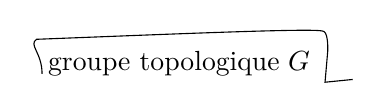
\begin{tikzpicture}[baseline=(phrase.base)]
\node[inner sep=0pt,anchor=base west] (phrase) at (0,0) {groupe topologique $G$};
\draw[line width=0.4pt]
 ([xshift=-2pt,yshift=1pt]phrase.south west)
 .. controls ([xshift=-2pt,yshift=4pt]phrase.west)
          and ([xshift=-7pt,yshift=2pt]phrase.north west)
 .. ([xshift=-4pt,yshift=4pt]phrase.north west)
 .. controls ([yshift=6pt]phrase.north)
          and ([yshift=8pt]phrase.north east)
 .. ([xshift=4pt,yshift=7pt]phrase.north east)
 .. controls ([xshift=6pt,yshift=7pt]phrase.north east)
          and ([xshift=6pt,yshift=2pt]phrase.north east)
 .. ([xshift=6pt]phrase.north east)
 -- ([xshift=5pt,yshift=-2pt]phrase.south east)
 -- ([xshift=15pt,yshift=-1pt]phrase.south east);
\end{tikzpicture}}
tel que \deleted{\unsure{$\widetilde A_0^\circ$}}\inserted{$G^\circ$} soit simplement connexe; \deleted{soit}
\deleted{\unsure{posons} $\mu=\mathrm{Centre}(\unsure{\widetilde A_0^\circ})$}
\[
(67)\qquad\Pi_1(G^\circ)=0
\]
soit
\[
(68)\qquad \mu=\mathrm{Centre}(G^\circ),\qquad\Gamma=G/G^\circ
\]
\margin{on suppose $\mu$ discret (donc $G^\circ$ s'identifie au groupe rev. universel de $G^\circ/\mu=\mathcal H^\circ$ (si $\mathcal H=G/\mu$))}
alors l'extension de groupes topologiques $G$
de $\Gamma$ par $G^\circ$ définit
\[
(69)\qquad\Gamma\longrightarrow\mathrm{Aut\,ext}(G^\circ)
\qquad(\longrightarrow\mathrm{Aut}(\mu).)
\]
et l'ens des classes d'extensions correspondantes
à une opération \inserted{extérieure} donnée de $\Gamma$ sur $G^\circ$
est de façon naturelle un torseur sous
$H^2(\Gamma,\mu)$ (s'il n'est vide, ce \unsure{qui est|qu'on a} exclu
par hypothèse de départ, en partant de $G$\ldots)
\margin{236}

\scanpage{238}
Cette catégorie d'extensions est d'ailleurs équivalente
\deleted{Elle \unsure{correspond}}
à celle des scindages d'une certaine
Gr.-catégorie définie par Sinh \inserted{via $(69)$}, dont les $\Pi_0$ et
$\Pi_1$ sont respectivement $\deleted{\unsure{\Pi_0}}\Gamma$ et $\mu$ --- laquelle
est \inserted{donc} ici scindée par la donnée de l'extension
$G$. (Dans le cas qui nous intéresse,
$\Gamma\simeq\mu\simeq\{\pm1\}$, et
cette extension est $\overline{\mathrm m}$ scindée, et correspond
à une opération d'ordre $2$ de $\Gamma$ sur $G^\circ$,
dont je doute fort que ce soit un autom intérieur.
En fait, j'ai l'impression que dans les
deux cas qui nous occupent ($\widetilde{\mathrm{GP}}(1,\mathbb C)$ et
$\widetilde A_0$) que $(69)$ est un \uline{iso}
$\Gamma=\{\pm1\}\xrightarrow{\sim}\mathrm{Autext}(G^\circ$

Ceci posé, la donnée d'un torseur sous
$\mathcal H=G/\mu$ définit $1^\circ$) un torseur sous $\Gamma$,
$\mathcal H\longrightarrow\Gamma\simeq\mathcal H/\mathcal H^\circ$; $2^\circ$) le groupoïde des
relèvements des relèvements de ce torseur
en un torseur sous $G$, qui est un
$\mu$-groupoïde \inserted{connexe} (sur lequel $\mu$ opère).
\margin{On suppose que $\Gamma$ opère \uline{trivialement} sur $\mu$ i.e. $\mu\subset\mathrm{Centre}(G)$}

Si on \deleted{\unsure{exp}} reprend en termes de fibrés
sur un espace de base $S$ on trouve
\margin{237}

\scanpage{239}
\mspage{120}
encore sur $S$ (pour tt $\mathcal H_S$-torseur topologique)
un couple $(\omega,\unsure{\mathcal R|R})$ d'un $\Gamma$-torseur, et d'
une $\mu$-gerbe sur $S$, qui sont décrits (à \unsure{isom.}
\inserted{\illegible{1} \unsure{équival.}}
\unsure{à équiv.|et équiv.} près) par $H^1(S,\Gamma)$ et $H^2(S,\mu)$
respectivement. On voudrait dégager des
conditions \inserted{sur $G$ et sur $S$} pour que l'application
\[
(70)\qquad H^1(S,\mathcal H)\longrightarrow H^1(S,\Gamma)\times H^2(S,\mu)
\]
soit bijective.
\margin{\uline{NB} $\omega$ ne dépend pas du choix de l'extension \unsure{$\widetilde G$} de $\mathcal H$ par \unsure{$\mathfrak z$|$\zeta$}${}\simeq\Pi_1(\mathcal H^\circ)$; \unsure{par contre} $\mathcal R$ en dépend (et il \unsure{faudrait} voir comment)}

Injectivité : Si l'image \inserted{d'un $\zeta\in H^1(S,\mathcal H)$,}
dans $H^2(S,\mu)$ est nulle,
l'élément de $H^1(S,\mathcal H)$ se relève en un élément $\widetilde\zeta$
de $H^1(S,\widetilde{\mathcal H}=G)$; \unsure{dont} l'image dans $H^1(S,\Gamma)$
\unsure{par} $G\longrightarrow\Gamma$ est la $\overline{\mathrm m}$ que celle de $\zeta$, donc si
elle est triviale, on voit que $\widetilde\zeta$ provient d'
un $\widetilde\zeta_0\in H^1(S,G^\circ)$. Si on sait que
$H^1(S,G^\circ)=(1)$, on gagne. Par les
marteaux-pilons d'homotopie, ça marche
si $\exists n\in\mathbb N$ avec
\[
\Pi_i(G^\circ)=0\quad\text{si}\quad i\leq n
\]
\inserted{(donc $\Pi_i(B_{G^\circ})=0$ si $i\leq n+1$)}
\deleted{$\Pi_i(S)=0$ si $i>n+1$}
\deleted{$\dim S\leq n+1$}
$S$ un CW-complexe de dim $\leq n+1$
\margin{dans le cas qui nous occupe, on peut prendre $n=2$}

Pour la surjectivité, notons que \unsure{pour|d'abord} un
\margin{238}

\scanpage{240}
élément de $H^2(S,\mu)$, l'obstruction à ce qu'il
se relève en un élément \inserted{$\zeta$} de $H^1(S,\mathcal H)$ est
dans $H^2(S,G)$ [par la suite exacte
de \unsure{coh.} associée : $1\longrightarrow\mu_S\longrightarrow G_S\longrightarrow\mathcal H_S\longrightarrow1$]
il faut exprimer qu'une certaine \deleted{\illegible{1}} gerbe
liée par $G_S$ est neutre --- brr!. Mais
partons plutôt de l'élément \inserted{\unsure{$\omega$|$\widetilde\zeta$}} de $H^1(S,\Gamma)$,
si l'extension de $\Gamma$ par \deleted{\unsure{$G^\circ$}}$\mathcal H^\circ$ est scindée, alors
on peut trouver un $\zeta_0\in H^1(S,\mathcal H_S)$ qui
donne naissance à \unsure{$\omega$}. Elle a une certaine
obstruction $\rho_0$ dans $H^2(S,\mu)$, et il s'agit
de corriger $\zeta_0$ en $\zeta$, \inserted{de} telle façon que
l'obstruction devienne $\rho\in H^2(S,\mu)$ donné.
\deleted{On dispose de} \inserted{Utilisant $\zeta_0$} pour tordre $\mathcal H_S$ en
$\mathcal H'_S$, et (via l'opération de $\mathcal H_S$ \inserted{$=G_S/\mu_S$} sur $G_S$,
compte tenu que $\mu_S\subset\mathrm{centre}\,G_S$) pour
tordre $G_S$ aussi \inserted{en $G'_S$}, d'où
\[
1\longrightarrow\mu\longrightarrow G'_S\longrightarrow\mathcal H'_S\longrightarrow1
\]
on trouve que les $\zeta$ ayant $\overline{\mathrm m}$ image dans $H^1(S,\Gamma)$
\margin{239}
\scanpage{241}
\mspage{121}
% l. 1
que \unsure{$\xi_0$} correspondent \inserted{$1-1$} aux
$\xi'\in H^1(S,\mathcal H'_S)$.
% A hatched loop with a descender stands under the H of H'_S (an overwritten letter, perhaps a G).

% l. 2
Pour un tel \deleted{\unsure{$\mathcal H'_S$}} $\xi'$, soit
$\delta'(\xi')\in H^2(S,\mu)$
% l. 3
l'obstruction à le relever en $H^1(S,\unsure{\mathcal G'_S|\mathcal G_S})$,
% l. 4
et $\delta(\xi')=\delta(\xi)$ l'obstruction à le relever
% l. 5
en $H^1(S,\mathcal G_S)$. Sauf erreur on a
% l. 6
\[
\delta'(\xi')=\delta(\xi')-\rho_0
\]
% l. 7
i.e.
\[
\delta(\xi')=\delta(\xi)=\delta'(\xi')+\rho_0
\]
% l. 8
et on veut $\delta(\xi)=\rho$ i.e.
% l. 9
\[
\deleted{\unsure{\delta(\xi')}=}\quad
\delta'(\xi')=\rho-\rho_0
\]
% l. 10
et la question revient encore à \deleted{\illegible{3}} \inserted{la}
% l. 11
surjectivité de $H^1(S,\mathcal H'_S)\longrightarrow H^2(S,\mu)$
\deleted{\illegible{1}}
% l. 12
--- je ne m'en tire pas. Il faudrait
% l. 13
consulter des gens compétents, comme
% l. 14
Giraud ou Larry Breen. On sent qu'il
% l. 15
faudrait travailler avec un Gr-champ $\underline{\underline{\mathcal H}}$
% l. 16
de coefficients, d'invariants $\underline{\pi}_0\simeq\Gamma$ et
$\underline{\pi}_1\simeq\mu$,
% l. 17
(mais pas nécessairement un champ de Picard!)
% l. 18
\deleted{avec} et
$H^1(S,\underline{\underline{\mathcal H}})\simeq\text{Classes d'applications}$
% l. 19
de $S$ dans $B\underline{\underline{\mathcal H}}$, qui est un espace
% l. 20
connexe avec $\pi_1(B\underline{\underline{\mathcal H}})\simeq\Gamma$,
$\pi_2(B\underline{\underline{\mathcal H}})=\mu$.
% l. 21
Ici la classe de \unsure{Postnikoff} dans $H^3(\Gamma,\mu)$ est nulle,
\margin{240}

\scanpage{242}
% l. 1
[mais peut-être n'y a-t-il pas lieu de
% l. 2
trop se raccrocher à cette hypothèse,
% l. 3
correspondant à l'existence d'une \inserted{ext.} $\mathcal G$ de $\mathcal H$
\inserted{par $\pi_1(\mathcal H^\circ)$} \deleted{\illegible{1}}
% l. 4
qui redonne l'extension universelle de
% l. 5
$\mathcal H^\circ$ par $\pi_1(\mathcal H^\circ)$] on a un \unsure{hom.}
% l. 6
$B\mathcal H$ \deleted{\illegible{1}} $\longrightarrow B\underline{\underline{\mathcal H}}$
qui induit un iso pour
% The struck mark stands under the first BH (perhaps a cancelled double underline).
% l. 7
les $\pi_i$ pour $i\leq2$, et pour $i\leq n$
(où $n\geq2$ \inserted{est donné})
% l. 8
sss $\pi_i(B\mathcal H)=0$ pour $2<i\leq n$, i.e.
% l. 9
$\pi_i(\mathcal H)=0$ pour $2\leq i\leq n-1$ [dans le cas
% l. 10
qui nous intéresse $\mathcal H=A_0$, on peut
% l. 11
prendre $n=3$). Ceci implique que pour
% l. 12
tout C-W-complexe $S$ de dim $\leq n$,
% l. 13
on a \inserted{(Hot désignant les morphismes dans
la cat. homotopique non ponctuée)}
% l. 14
\[
\mathrm{Hot}(S,B\mathcal H)\xrightarrow{\sim}
\mathrm{Hot}(S,B\underline{\underline{\mathcal H}})
\]
% l. 15
\unsure{c.à.d.|i.e.}
\[
H^1(S,\mathcal H)\xrightarrow{\simeq}
H^1(S,\deleted{\unsure{B}}\underline{\underline{\mathcal H}})
\]

% l. 16
Mais si l'invariant de \unsure{Postnikoff}-Sinh
% l. 17
$\unsure{K|k}\in H^3(\Gamma,\mu)$ est nul,
\deleted{\illegible{1}} (ainsi que l'action
% l. 18
de $\Gamma$ sur $\mu$) alors sauf erreur
$B\underline{\underline{\mathcal H}}$ s'iden%
% l. 19
tifie à un produit $K(\Gamma,1)\times K(\pi,2)$,
\deleted{et}
% l. 20
(cette ``identification'' dépendant justement du
\margin{241}

\scanpage{243}
\mspage{122}
% l. 1
choix des $H^2(\pi_1,\pi_2)\simeq H^2(\Gamma,\mu)$ !), et par
% l. 2
suite
\[
H^1(S,\underline{\underline{\mathcal H}})\xrightarrow{\simeq}
H^1(S,\Gamma)\times H^2(S,\mu)
\]
% l. 3
pour tt espace $S$, donc pour $S$ un C-W-%
% l. 4
complexe de dim $\leq n$
% l. 5
\[
(71)\qquad
H^1(S,\mathcal H)\xrightarrow{\simeq}H^1(S,\Gamma)\times H^2(S,\mu)
\]

% l. 6
Donc la classification des fibrés en sphères
% l. 7
topologiques sur un espace topologique $S$,
% l. 8
pour un C-W complexe $S$ de dim $\leq3$,
% l. 9
marche bel et bien. Bien entendu, le
% l. 10
fait qu'on soit obligé ici de se borner à
% l. 11
des \deleted{\illegible{1}} $S$ de dim $\leq3$ tient au fait
% l. 12
que nous n'avons trouvé \deleted{\unsure{qu'}}
(via $\underline{\underline{\mathcal H}}$)
% l. 13
qu'une description $2$-isotopique (et non
% l. 14
$\infty$-isotopique) de la catégorie des $2$-sphères
% l. 15
topologiques.

% l. 16
Je voudrais reprendre la classification
% l. 17
pour un CW-complexe $S$ quelconque, en
% l. 18
utilisant le fait que l'inclusion
% l. 19
\[
\widetilde{\mathrm{GP}}(1,\mathbb C)\hookrightarrow A_0
\]
\margin{242}

\scanpage{244}
% l. 1
est une équivalence d'homotopie, et induit
% l. 2
donc une bijection
% l. 3
\[
H^1(S,\widetilde{\mathrm{GP}}(1,\mathbb C))\longrightarrow H^1(S,A_0)
\]
% l. 4
et $\overline{\mathrm m}$ une $\infty$-équivalence des $\infty$-catégories des
% l. 5
\deleted{fibrés} \inserted{torseurs} sur $S$, de \deleted{\illegible{1}} groupes
$\widetilde{\mathrm{GP}}$ (correspondant
% l. 6
aux fibrés en sphères conformes, ou en
% l. 7
droites projectives sur une \deleted{corps} $\mathbb R$-algèbre
\inserted{(non précisée)}
% l. 8
isomorphe à $\mathbb C$) et de groupe $A_0$ --- correspondant
% l. 9
aux fibrés en sphères sur $S$.

% l. 10
Le premier invariant d'un fibré de groupe $\widetilde{\mathrm{GP}}$
% l. 11
est un \deleted{fibré} torseur \unsure{$\eta$|$T$} sous $(\mathbb Z/2\mathbb Z)_S$
\deleted{\illegible{2}} défini (\unsure{à isom.}
% l. 12
\uline{non unique} \inserted{près) par un} $\chi\ (\in H^1(S,\mathbb Z/2\mathbb Z))$.
% Physical order: "non unique" opens l. 12 under "est un"; "près) par un" is raised after the
% parenthesis of H^1; linearised as the sense requires.
\margin{i.e. un \unsure{rev. étale|rev. double} de degré $2$.
La donnée de \unsure{$\eta$|$\chi$} revient à la donnée d'un système \unsure{$T$} d'entiers
tordus sur $S$.}
% l. 13
\inserted{Ce torseur} servira à tordre $\mathbb C$
(via l'opération \inserted{fidèle} de $\mathbb Z/2\mathbb Z$ sur
% l. 14
la $\mathbb R$-extension $\mathbb C$), \deleted{et} d'où un fibré loc.
\deleted{\illegible{1}}
% l. 15
constant en \deleted{corps} extensions \inserted{quadratiques}
de $\mathbb R$ \deleted{\illegible{1}},
% l. 16
soit $C$, et on \deleted{prendra le} enrichira $S$
% l. 17
par le faisceau \inserted{$\underline C_S$ (ou $\underline C$)} des sections continues de
% l. 18
$C$ (ce qui est une façon de tordre
% l. 19
\deleted{$\mathrm{Sl}(2,$} $\mathrm{GP}(1,\mathbb C)_S$
en $\mathrm{GP}(1,C)_S=\mathrm{GP}(1,\underline C)$))
% l. 20
et il s'agit de \deleted{\unsure{donc}} décrire de façon
% l. 21
compréhensible \deleted{la catégorie} \inserted{--- en passant} au besoin,
% l. 22
aux \deleted{\unsure{$\infty$}}$n$-isotopiques, pour $n=\ldots$ --- la catégorie
\margin{243}

\scanpage{245}
\mspage{123}
% l. 1
--- dépendant du choix de $\chi$ via $\underline C$ --- des
% l. 2
algèbres d'Azumaya de rang $4$ sur $\underline C$,
% l. 3
ou encore des fibrés en droites projectives
% l. 4
sur $\underline C$, ou des torseurs sous $\mathrm{GP}(1,\underline C)$.

% l. 5
Or utilisant \deleted{$\mathrm{Sl}(2,\underline C)\longrightarrow
\mathrm{GP}(1,\underline C$} \inserted{la suite \unsure{ex.te}}
% l. 6
\[
1\longrightarrow\mu_{2S}\longrightarrow\mathrm{Sl}(2,\underline C_S)
\longrightarrow\mathrm{GP}(1,\underline C_S)\longrightarrow1
\]
% l. 7
on associe à un objet de la catégorie
% l. 8
--- disons un torseur sous $\mathrm{GP}(1,\underline C_S)$ --- la
% l. 9
catégorie \inserted{fibrée (sur des ouverts variables de $S$)} de ces relèvements à
$\mathrm{Sl}(2,\underline C_S)$,
% l. 10
qui est une \uline{gerbe} \inserted{$\mathcal G$} liée par $\mu_2$.
% l. 11
C'est cette gerbe qui est le deuxième
% l. 12
invariant complet --- plus fin que
% l. 13
sa classe \deleted{dans $H^2($} \inserted{d'équivalence, qui s'identifie à un}
% l. 14
$\xi\in H^2(S,\mu_2)=H^2(S,\{\pm1\})$
(jouant le rôle
% l. 15
d'un groupe de Brauer)

% l. 16
Un isomorphisme de fibrés, d'invariants
% l. 17
$(T,\mathcal G)$, $(T',\mathcal G')$, définira un isom $T\simeq T'$
% l. 18
(d'où un isom \deleted{$\mathrm{GP}(1,C$}
$\underline C_T\simeq\underline C_{T'}$ d'où
% l. 19
un isom $\mathrm{GP}(1,\underline C_T)\simeq\mathrm{GP}(1,\underline C_{T'})$) --- et
% l. 20
une équivalence de gerbes --- il faudrait
\margin{244}

\scanpage{246}
% l. 1
expliciter que pour deux isomorphismes
% l. 2
$f,g$ des torseurs, \deleted{et} d'où
% l. 3
\diagram{\begin{tikzcd}[ampersand replacement=\&,column sep=3.4em]
f_T,g_T:\ T
 \arrow[r,shift left=2.6ex,line width=0.7pt,"\unsure{\simeq}"]
 \arrow[r,phantom,"\unsure{\deleted{\xrightarrow{\sim}}}" description]
 \arrow[r,shift right=2.6ex,"\sim"]
\& T'
\& f_{\mathcal G},g_{\mathcal G}:\mathcal G
 \arrow[r,shift left=1.6ex,"\unsure{\simeq}"]
 \arrow[r,shift right=1.6ex,"\unsure{\simeq}"]
\& \mathcal G'
\end{tikzcd}}
% l. 4
et pour tte homotopie $h_t$ $(0\leq t\leq1)$ de
% l. 5
$f$ à $g$, on trouve $f_T=g_T$ et un
% l. 6
isom $h_*:f_{\mathcal G}\xrightarrow{\sim}g_{\mathcal G}$ d'équivalences de
% l. 7
gerbes, qui ne dépend que de la classe
% l. 8
d'homotopie de cette homotopie. On
% l. 9
trouve ainsi une $2$-foncteur, de la
% l. 10
$2$-catégorie des \deleted{fibrés} torseurs sur $S$
% l. 11
de groupe $\widetilde{\mathrm{GP}}(1,\mathbb C)$, vers la $2$-catégorie
% l. 12
formée des couples \inserted{$(T,\mathcal G)$} d'un
\deleted{torseur} \inserted{système} d'%
% l. 13
entiers tordus, \deleted{et} ($\Longleftrightarrow$ d'un torseur sur
% l. 14
$S$ de groupe \deleted{\illegible{1}} \inserted{$\mathbb Z/2$}) et d'une
% l. 15
\deleted{\unsure{$\{\pm1\}=$}} $\mu_2(\mathbb C)$-gerbe $\mathcal G$ sur $S$. Ce
% l. 16
$2$-foncteur, sauf erreur, est $2$-fidèle
% l. 17
sous les conditions explicitées plus
% l. 18
haut (\deleted{\illegible{2}} (dim $S\leq4$), et
% l. 19
est $3$-fidèle (i.e. l'application injective
% l. 20
$H^1(S,\widetilde{\mathrm{GP}})\unsure{\longrightarrow|{-}}
H^1(S,\mathbb Z/2\mathbb Z)\times H^2(S,\mu_2)$ est surjective)
\margin{245}

\scanpage{247}
\mspage{124}
% l. 1
si on a même dim $S\leq3$. On s'attend qu'elle
% l. 2
soit $1$-fidèle dès que dim $S\leq5$, $0$-fidèle
% l. 3
dès que dim $S\leq6$.
\margin{??}
% A vertical marginal stroke accompanies approximately lines 1--3.
[\uline{NB} \inserted{l'assertion} ``$0$-fidèle'' signifie
% l. 4
que si \inserted{ci-dessus} on a deux homotopies $h,h'$ de $f$ à $g$,
% l. 5
telles que $h_*=h'_*,$ alors $h$ et $h'$ sont homotopes.
% l. 6
La condition ``$1$-fidèle'' signifie \inserted{$0$-fidèle et} que tout
% l. 7
isom de $f_{\mathcal G}$ à $g_{\mathcal G}$
\deleted{\unsure{provient d'un}} est de la
% l. 8
forme $h_*$ (avec $h$ bien déterminé à hom. près,
% l. 9
par la condition précédente de $0$-fidélité). La
% l. 10
condition $2$-fidèle signifie que \inserted{de plus, pour} toute
\deleted{équivalence}
% l. 11
\deleted{\unsure{donnés}} $\varphi:T\simeq T'$,
$\psi_{\mathcal G}:\mathcal G\xrightarrow{\approx}\mathcal G'$,
il existe
% l. 12
un isom de fibrés $f$ tel que $\varphi=f_T$,
\deleted{$\psi$ \illegible{1}}
% l. 13
et un isom $\psi\simeq f_{\mathcal G}$. Enfin $3$-fidèle signifie
% l. 14
que de plus, pour tout couple $T,\mathcal G$,
% l. 15
$\exists\ T',\mathcal G'$ provenant d'un fibré, \deleted{et de}
% l. 16
et un isom $T\simeq T'$ et une équivalence
% l. 17
$\mathcal G\approxeq\mathcal G'$. Ces notions catégoriques
% l. 18
doivent interpréter simplement que, si
% l. 19
on regarde $\mathcal H=\widetilde{\mathrm{GP}}(1,\mathbb C)
\xrightarrow{\alpha}\underline{\underline{\mathcal H}}$
--- où $\underline{\underline{\mathcal H}}$
% l. 20
est déduit de $\mathcal H$ en ``tuant les \unsure{g\textsuperscript{o}-pes}
% l. 21
d'homotopie $\pi_i$ pour $i\geq2$'', de sorte que
\margin{246}

\scanpage{248}
% l. 1
$\alpha$ induit un isom des $\pi_i$ pour $i\leq1$
% l. 2
(et $\overline{\mathrm m}$ pour $i\leq n$ si
$\pi_i(\mathcal H)=0$ pour $1<i\leq n$)
% l. 3
\deleted{et $B_\alpha$ un} d'où
% l. 4
\[
B_\alpha:B\mathcal H\longrightarrow B\underline{\underline{\mathcal H}}
\]
\margin{\uline{NB} $B\underline{\underline{\mathcal H}}$ est déduit de
$B\mathcal H$ en tuant les $\pi_i$ pour $i\geq3$.}
% l. 5
(induisant un isom des $\pi_i$ pour $i\leq n+1$),
% l. 6
alors prenant pour \deleted{tout} \inserted{un espace donné} $S$ l'application
% l. 7
correspondante des espaces d'applications continues
% l. 8
\[
\deleted{\mathrm{Hot}}
\underline{\mathrm{Cont}}(S,B\mathcal H)
\unsure{\longrightarrow|{-}}
\underline{\mathrm{Cont}}(S,B\underline{\underline{\mathcal H}})
\]
% l. 9
celle ci induit un isom pour les
% l. 10
$\pi_i$ $(0\leq i\leq2)$. \deleted{\unsure{Comme}} Il semblerait que
% l. 11
$0$-fidélité est une condition d'injectivité
% l. 12
pour les $\pi_2$, $1$-fidèle la bijectivité pour les
% l. 13
$\pi_2$ et l'injectivité pour les $\pi_1$, $2$-fidèle
% l. 14
la bijectivité pour $\pi_2$ et $\pi_1$ et l'injectivité
% l. 15
pour $\pi_0$, $3$-fidèle la bijectivité pour $\pi_0,\pi_1,\pi_2$.

% l. 16
Comme $\pi_i(\mathrm{Cont}(S,B))\simeq
\pi_0(S\times S^i,B)$,
% l. 17
\deleted{on voit} \inserted{il semblerait}
qu'on est conduit, pour la $0$-%
% l. 18
fidélité, de faire l'hypothèse draco%
% l. 19
nienne que $S\times S^2$ de dim $\leq4$, pour la
% l. 20
$1$-fidélité que $S\times S^2$ de dim $\leq3$ i.e. $S$
% l. 21
de dim $\leq1$ ? (\unsure{Ceci|Cela} impliquerait alors
% l. 22
la $3$-fidélité\ldots)
\margin{247}

\scanpage{249}
\mspage{125}
% l. 1
Prenons l'analogue arithmétique, d'une description
% l. 2
(plus ou moins ``fidèle'') \deleted{par \illegible{1}}
de nature ``profinie''
% l. 3
des droites projectives \deleted{définies} (éventuellement
% l. 4
tordues) définies sur un corps de type
% l. 5
fini $K$ \inserted{sur $\mathbb Q$ (plus gén. sur un schéma $S$ quelc.)},
celles ci forment a priori une catégorie
% l. 6
sans plus --- un groupoïde (pas nécessairement
% l. 7
connexe) je ne sais pas en faire une
% l. 8
$2$-catégorie raisonnablement, car pour deux
% l. 9
isom $f,g$ \inserted{$(=f\circ u)$} de tels torseurs, définir les
% l. 10
homotopismes de $f$ à $g$, i.e. pour une ``forme''
% l. 11
$G$ de $\mathrm{GP}(1)_S$ et une section $u$ de $G$,
% l. 12
définir les ``homotopies'' de $u$ à l'%
% l. 13
identité, \deleted{et les classes \inserted{d'homotopie} de telles \illegible{1}}
\inserted{ou plutôt} une
% l. 14
notion qui remplace la notion de classe d'%
% l. 15
homotopie de telles homotopies. \deleted{Mais} \inserted{Ce serait}
% l. 16
sans doute un relèvement de $u$ en une
\deleted{
% l. 17
\unsure{Si} $S$ est \illegible{1} d'un pt géométrique
% l. 18
\illegible{1} \unsure{tte section} définit une \illegible{1}
% l. 19
\unsure{si $K$ est alg.} Pour un corps de base
% l. 20
alg. clos \unsure{tout au moins} (les \unsure{sections}
% l. 21
définissant un pt géométrique) on
% l. 22
peut songer à prendre les ``classes de
% l. 23
chemins de $f$ à \illegible{1} de $u$ à
}
% l. 24
section du \deleted{\unsure{$\widetilde{\mathrm{GP}}$}}
revêtement simplement
% l. 25
connexe $\widetilde G$ de $G$ !
\margin{248}

\scanpage{250}
% l. 1
je tiens là quelque chose d'assez amusant,
% l. 2
mais que je ne vais pas poursuivre --- de
% l. 3
\unsure{toutes façons|toute façon} il est clair que la ``description''
% l. 4
des droites projectives (sur un corps de
% l. 5
type fini disons) à laquelle on aboutit,
% l. 6
n'a rien de fidèle --- pas même $0$-fidèle !
% l. 7
Ainsi tous les autom de $\mathbb P^1_K$ provenant de
% l. 8
$\mathrm{Sl}(2,K)$ seront identifiés à l'identité ---
% l. 9
c'est un peu brutal ! Mais je me
% l. 10
rends compte que le travail conceptuel
% l. 11
autour des thèmes ``Brauer'' n'est pas
% l. 12
terminé --- qu'il y a à comprendre
% l. 13
des choses pour l'étude de la catégorie
% l. 14
(\inserted{qui devrait être} une \uuline{2}-catégorie !)
des Algèbres d'Azumaya
% l. 15
\deleted{\unsure{de}} degré \uline{fixé} (ici $4$)\ldots
\margin{249}
\scanpage{251}
\mspage{126}

\uline{21 Lien avec les espaces de Teichmüller.}

D'abord un complément lié au diagramme \inserted{d'inclusions} (31) du n° 19, dans lequel \(A_{g,(\nu,\nu+1)}\) mérite la notation plus simple \(A_{g,\nu}^{\bullet}\) (\unsure{groupe} des autom. de \(U_{g,\nu}\) ponctué par \(a_{g,\nu}\)). Considérons \unsure{l'inclusion|la filtration} des sous-groupes de \(A_g\)
\[
 A_{g,\nu}^{\circ}\supset B_{g,\nu}\supset A_{g,\nu+1}^{\circ}
 \tag{72}
\]
\deleted{\unsure{\(A_{g,\nu}^{\bullet}\)}}

\unsure{donnant}, en divisant par \(A_{g,\nu+1}\) et dans le cas anabélien \(2g+\nu\geq 3\), la fibration

(73) \diagram{\begin{tikzcd}[ampersand replacement=\&]
\widetilde U_{g,\nu} \arrow[r] \& U_{g,\nu} \\
A_{g,\nu}^{\circ}/A_{g,\nu+1}^{\circ} \arrow[u, phantom, "\unsure{\simeq}" description] \&
\end{tikzcd}}

On cherche le plus grand ss-groupe de \(A_g\) qui normalise \unsure{ces|les} triplet (72), et qui \deleted{\unsure{définit}} \inserted{opère} donc \deleted{\unsure{sur}} la fibration \(\widetilde U_{g,\nu}\to U_{g,\nu}\) (où \(\widetilde U_{g,\nu}\) est le rev. universel de \(U_{g,\nu}\) basé en \(a_{g,\nu}\)); comme les normalisateurs de \(A_{g,\nu}^{\circ}\) et \(A_{g,\nu+1}^{\circ}\) respectivement sont \(A_{g,\nu}\) et \(A_{g,\nu+1}\), le groupe en question doit être contenu dans leur intersection \(A_{g,\nu}^{\bullet}\), lequel normalise \deleted{\unsure{également}} \(B_{g,\nu}=A_{g,\nu}^{\bullet}\cap A_{g,\nu}^{\circ}\). \unsure{C'est} donc ce groupe qu'il y a lieu de faire opérer sur la fibration (73) -- le sous-groupe \unsure{formé} \deleted{\illegible{7} \(U_{g,\nu}\)} \inserted{des éléments de \(A_{g,\nu}\)} dont l'opération

\scanpage{252}

sur \(U_{g,\nu}\) est isotope à l'identité étant \unsure{justement} \(B_{g,\nu}\) -- donc c'est le groupe \unsure{\(\Gamma\)}
\[
 A_{g,\nu}^{\bullet}/B_{g,\nu}\simeq\Gamma_{g,\nu}
\]
qui, comme de juste, opère à isotopie près. On voudrait décrire le groupe de tous les autom. de la fibration topologique \(\widetilde U_{g,\nu}\) sur \(U_{g,\nu}\) qui sera a priori une extension du groupe
\[
 \begin{aligned}
 A_{g,\nu}&=\operatorname{Aut}(U_{g,\nu})\quad\text{par}\quad
 \Pi_{g,\nu}=\pi_1(\unsure{U_{g,\nu}|\widetilde U_{g,\nu}},a_{g,\nu})\\
 &=\operatorname{Aut}_{U_{g,\nu}}(\widetilde U_{g,\nu}).
 \end{aligned}
\]

\deleted{\illegible{1}} Cette extension \inserted{est \uline{\unsure{scindée can\textsuperscript{t}}}} \deleted{\unsure{splittée}} sur \(A_{g,\nu}^{\bullet}\), \inserted{stabilisateur au pt base \(a_{g,\nu}\)} (et on retrouve ainsi l'op. de \(A_{g,\nu}^{\bullet}\) pour la fibration (73). Or on a déjà une extension \(\Gamma'_{g,\nu+1}\) de \(\Gamma_{g,\nu}\) par \(\Pi_{g,\nu}\), d'où par image inverse par \(A_{g,\nu}\to\Gamma_{g,\nu}=A_{g,\nu}/A_{g,\nu}^{\circ}\), une extension (que je vais noter \(\widetilde A_{g,\unsure{\nu}}\)) de \(A_{g,\nu}\) par \(\Pi_{g,\nu}\) :
\[
 \widetilde A_{g,\nu}\simeq A_{g,\nu}\mathbin{\times}_{\Gamma_{g,\nu}}\Gamma'_{g,\nu+1}
 \tag{74}
\]
\(=\) groupe quotient du ss-groupe \deleted{\unsure{\(H\)}} \(\widetilde A_{g,\nu}^{\unsure{\natural|\sharp}}\) \unsure{de} \(A_{g,\nu}\times A_{g,\nu}^{\bullet}\) formé des couples \((u,v)\), \(u\unsure{\equiv}v\) \deleted{\unsure{\(A_{g,\nu}^{\circ}\)}} mod. \(A_{g,\nu}^{\circ}\), par le sous-groupe \deleted{\unsure{\(B_{g,\nu}^{\circ}\)}} \(1\times A_{g,\nu+1}^{\circ}\).

On a donc deux \inserted{(et = trois!)} structures d'extensions sur \(\widetilde A_{g,\nu}\)

(75) \diagram{\begin{tikzcd}[ampersand replacement=\&][column sep=small]
1 \arrow[r] \& \Pi_{g,\nu} \arrow[r] \& \widetilde A_{g,\nu} \arrow[r,"p"] \& A_{g,\nu} \arrow[r] \& 1 \\
1 \arrow[r] \& A_{g,\nu}^{\circ} \arrow[r] \& \widetilde A_{g,\nu} \arrow[r] \& \Gamma'_{g,\nu+1} \arrow[r] \& 1
\end{tikzcd}}
\diagram{\begin{tikzcd}[ampersand replacement=\&][column sep=small]
1 \arrow[r] \& (A_{g,\nu}^{\circ}\unsure{\times|\rtimes}\Pi_{g,\nu}) \arrow[r] \& \widetilde A_{g,\nu} \arrow[r] \& \Gamma_{g,\nu} \arrow[r] \& 1
\end{tikzcd}}

\margin{\uline{NB.} Le deuxième \unsure{veut exprimer} que \(\widetilde A_{g,\nu}^{\circ}=A_{g,\nu}^{\circ}\) et \(\pi_0(\widetilde A_{g,\nu})\simeq\Gamma'_{g,\nu+1}\) (l'ex. can. de \(\Gamma_{g,\nu}\) par \(\Pi_{g,\nu}\)).}
\deleted{\unsure{Or}}

\scanpage{253}
\mspage{127}

Je voudrais faire opérer \(\widetilde A_{g,\nu}\) sur \(\widetilde U_{g,\nu}\), i.e. faire \deleted{\illegible{1}} opérer \(H=\widetilde A_{g,\nu}^{\unsure{\natural|\sharp}}\) \unsure{en opérat.} \deleted{de façon que \((u,v)\)} triviale de \(A_{g,\nu+1}^{\circ}\), et ceci en respectant les conditions suivantes

\margin{\unsure{donnée triviale} sur \(1\times A_{g,\nu+1}^{\circ}\). Cf généralisation ci-dessous en marge.}

a) \deleted{\illegible{1}} (compatibilité avec \(\widetilde A_{g,\nu}\to A_{g,\nu}\)) le couple \((u,v)\in H\) opère \unsure{sur} \(\widetilde U_{g,\nu}\) par un autom. compatible avec l'automorphisme \inserted{\(u\) de} \(U_{g,\nu}\) (on dira que c'est un \(u\)-autom.).

b) (compatibilité avec \(\Pi_{g,\nu}\to\widetilde A_{g,\nu}\)) Si \(u=1\), \inserted{[donc \(v\in A_{g,\nu}^{\circ}\), donc (comme \(v\in A_{g,\nu}^{\bullet}\)) \(v\in B_{g,\nu}\)]} alors l'opération de \((u,v)=(1,v)\) sur \(\widetilde U_{g,\nu}\) n'est autre que celle définie par \(v\bmod B_{g,\nu}^{\circ}=A_{g,\nu+1}^{\circ}\), qui est un élément de \(\Pi_{g,\nu}\simeq\operatorname{Aut}(\widetilde U_{g,\nu}/U_{g,\nu})\), ou encore, c'est celle définie par \uline{translation} \inserted{\uuline{à droite}} par \(\unsure{v^{-1}}\).

\margin{donnée de l'op. sur \(1\times B_{g,\nu}\).}

c) Compatibilité avec \deleted{\unsure{\(\widetilde A_{g,\nu}\to\Gamma'_{g,\nu+1}\)}} l'opération déjà \deleted{\illegible{1}} \inserted{obtenue plus haut} de \(A_{g,\nu}^{\bullet}\) sur \(\widetilde U_{g,\nu}\) : si \((u,v)\in H\) est tel que \(u=v\) (donc \(u=v\in A_{g,\nu}^{\bullet}\)) alors \(\unsure{(u,v)}=(u,u)\) opère \unsure{via} l'autom. int. défini par \(u\).

\margin{donnée de l'opération sur \(\delta(A_{g,\nu}^{\bullet})\) (\(\delta\) : flèche diagonale).}

d) \inserted{Compatibilité avec \(A_{g,\nu}^{\circ}\to\widetilde A_{g,\nu}\) :} L'opération de \(A_{g,\nu}^{\circ}\) sur \(\widetilde U_{g,\nu}\) est continue (ce qui, joint à a), détermine cette opération de manière unique \deleted{\illegible{2}} \inserted{et} l'existence \inserted{\unsure{a priori d'une telle op.}} (résulte de \(\pi_1(A_{g,\nu}^{\circ})=0\))).

\margin{donnée de l'opération sur \((A_{g,\nu}^{\circ})\times 1\).}

\unsure{tt} élément \inserted{\((u,v)\)} de \(H\) s'écrit de manière unique comme produit d'un élément \inserted{\((v,v)\)} de \(\delta(A_{g,\nu}^{\bullet})\), par un élément \inserted{\((v^{-1}u,1)\)} de \(A_{g,\nu}^{\circ}\times 1\) (le premier groupe normalisant le deuxième)

\margin{\uline{NB} L'opération de \(A_{g,\nu}^{\circ}\times 1\) se \unsure{décrit} le plus simplement par \uline{translations} de \unsure{\(A_{g,\nu}^{\circ}\)} sur l'espace \unsure{homogène} \(\widetilde U_{g,\nu}\) de \(A_{g,\nu}^{\circ}\).}

\scanpage{254}

et une opération de ce produit \(\frac12\) direct est donnée \inserted{bel et bien} par \deleted{\illegible{1}} la donnée d'opérations des deux groupes facteurs, satisfaisant une condition de compatibilité, qui est vérifiée ici par transport de structure. On a bien défini une opération de \(H=\widetilde A_{g,\nu}^{\unsure{\natural|\sharp}}\) sur la fibration (73), \deleted{\illegible{2}} satisfaisant les conditions c) et d) par construction même, il reste à vérifier a) et b).

Or pour a), il suffit de la vérifier séparément pour les \unsure{éléts} de \(H\) de \(\delta(A_{g,\nu}^{\bullet})\) et de \(A_{g,\nu}^{\circ}\times 1\), où c'est trivial par construction dans les deux cas. Reste à vérifier b), i.e. à expliciter l'opération d'un \unsure{élmt} \((1,v)\), \(v\in B_{g,\nu}\), qu'on écrit comme
\[
 (\qquad (1,v)=\deleted{(\unsure{v^{-1}},1)}(v,v)(v^{-1},1)
\]
donc
\[
 \rho\deleted{_{\unsure{\widetilde A}_{g,\nu}}}(1,v)=\rho(v,v)\rho(v^{-1},1).
\]

Or \(\rho(v,v)\) est induit par \(\operatorname{int}(v)\), \inserted{i.e. \(x\mapsto vxv^{-1}\)} et \(\rho(v^{-1},1)\) par translation à gauche : \(x\mapsto v^{-1}x\), donc le composé opère par \(x\mapsto xv^{-1}\). Ouf !

\scanpage{255}
\mspage{128}

On suppose maintenant que \(X_g\) est muni d'une structure \(C^\infty\), et on remplace dans les considérations \deleted{Soit} précédentes les groupes d'homéomorphismes par des groupes de difféomorphismes.

\margin{\uline{NB} Structure \(C^{\unsure{\nu|r}}\) avec \(\unsure{\nu|r}\geq 2\) suffirait}
\[
 \begin{aligned}
 E_g={}&\text{ens. des structures \deleted{complexes} \inserted{conformes}}\\
 &\text{sur }X_g\text{ compatibles avec sa}\\
 &\text{structure }C^\infty
 \end{aligned}
 \tag{76}
\]

\deleted{\unsure{Alors}} On voit de suite que \(E_g\) est un espace topologique \uline{\(\infty\)-connexe}, comme quotient de l'espace \(\infty\)-connexe \inserted{(un convexe)} des structures riemanniennes, par le \deleted{\unsure{gr.}} groupe \(\infty\)-connexe des applications \(C^\infty\) de \(X_g\) dans \(\mathbb R^{+*}\). Sur \(E_g\) le groupe \(A_g\) opère -- mais bien sûr \(E_g\) n'est plus un espace homogène. Notons tout de suite
\[
 \begin{aligned}
 E_g/A_g\simeq{}&\text{ens. des classes d'isomorphie}\\
 &\text{des \deleted{courbes algébriques} \inserted{surfaces} \deleted{\unsure{compactes}}}\\
 &\text{conformes compactes orientables}\\
 &\text{de genre }g
 \end{aligned}
 \tag{77}
\]

Et si on choisit une des deux orientations de \(X_g\), de sorte que \(E_g\) s'identifie à l'ens des structures \uline{complexes} sur \(X_g\) compatibles avec sa structure \(C^\infty\) \inserted{et son orientation}, alors \(E_g/A_g\) s'identifie à l'espace des classes d'isomorphie de courbes complexes \inserted{(non singulières) connexes} compactes de genre \(g\), \uline{modulo} passage à la complexe conjuguée. D'autre part

\scanpage{256}

\[
 \begin{aligned}
 E_g/A_g^+\simeq{}&\text{ens. des classes d'iso.}\\
 &\text{de courbes }\mathbb C\text{-alg \inserted{lisses} projectives}\\
 &\text{connexes de genre }g.
 \end{aligned}
 \tag{78}
\]

Plus généralement

\[
 \begin{aligned}
 E_g/A_{g,\nu}\simeq{}&\text{ens. des classes d'isomorphie}\\
 &\text{des \deleted{structures} \deleted{sur les} surfaces compactes}\\
 &\text{\inserted{conformes} munies \unsure{de multiponctures|de multiponctuations}}\\
 &\text{de type }(g,\nu)
 \end{aligned}
 \tag{79}
\]

\[
 \begin{aligned}
 E_g/A_{g,\nu}^{+}\simeq{}&\text{ens. des classes d'iso.}\\
 &\text{des courbes \deleted{\unsure{complexes}} \inserted{\(\mathbb C\) algébriques}}\\
 &\text{[lisses projectives connexes}\\
 &\text{de genre }g\text{] \uline{munies} d'une}\\
 &\text{multiponctuation, de type}\\
 &(g,\nu)
 \end{aligned}
 \tag{80}
\]
\margin{si \(X_g\) orientée.}

Ce sont là les ``espaces modulaires grossiers'' (``coarse moduli'' de Mumford), qu'on peut noter \(M_g^{\unsure{\natural|\sharp}}\) et \(M_{g,\nu}^{\unsure{\natural|\sharp}}\), et qui sont justement trop grossiers pour les usages géométriques les plus importants. \deleted{Mais} Beaucoup plus intéressants sont les quotients \(E_g/A_{g,\nu}^{\circ}\), \illegible{1}

\scanpage{257}
\mspage{129}

\[
 \widetilde M_{g,\nu}=E_g/A_{g,\nu}^{\circ}
 \qquad
 (\widetilde M_g=\widetilde M_{g,0}=E_g/A_g^{\circ})
 \tag{81}
\]
sur lesquels opère le groupe \deleted{\illegible{1}}
\[
 \Gamma_{g,\nu}=A_{g,\nu}/A_{g,\nu}^{\circ}
\]
par passage au quotient de l'op. de \(A_{g,\nu}\).

\deleted{\illegible{1}} L'espace \(\widetilde M_{g,\nu}\) \inserted{(avec l'opération de \(\Gamma_{g,\nu}\))} est appelé \uline{l'espace de Teichmüller} de type \(g,\nu\). Bien sûr on retrouve \(M_{g,\nu}^{\unsure{\natural|\sharp}}\) à partir de \(\widetilde M_{g,\nu}\) et \margin{\deleted{(82)}} de l'opération de \(\Gamma_{g,\nu}\) dessus, par
\[
 M_{g,\nu}^{\unsure{\natural|\sharp}}=\widetilde M_{g,\nu}/\Gamma_{g,\nu}
 \tag{\unsure{82}}
\]

\uline{Théorème} (Teichmüller) L'espace de Teichmüller \(\widetilde M_{g,\nu}\) est homéomorphe à \deleted{\(\mathbb R\)} \(\mathbb C^\mu\), où \(\mu=3g-3+\nu\) (\inserted{dans les} cas anabélien \(2g+\nu\geq 3\)), et \(\mu=3g-3+(\unsure{\nu}+\delta)\)
\[
 \delta=\dim_{\mathbb C}G
\]
dans le cas général, \(G\) étant \unsure{groupe} des autom. algébriques d'une \(U_{g,\nu}\) complexe (donc \(\delta=1\) dans les cas \unsure{``limites''} \((1,0)\) et \((0,2)\), et \inserted{plus \unsure{généralement}} \(\delta\) augmente de 1 chaque fois \unsure{pour} \(g\) fixé, et \((g,\nu-1)\) abélien, qu'on passe de \(\nu\) à \(\nu-1\)), donc

\margin{On peut dire aussi que \(\mu=3g-3+\nu'\), où \(\nu'=\nu\) dans le cas \unsure{anabélien}, et \unsure{où \(\nu'\)} dans le cas ``général'' est le plus petit entier \(\geq\nu\) tel que \((g,\nu')\) soit \unsure{``anabélien''}.}

\scanpage{258}

\[
 \left\{
 \begin{aligned}
 \mu&=1\quad\text{dans le cas }(1,0)\\
 \mu&=0\quad\text{dans les cas }(0,2),(0,1),(0,0),
 \end{aligned}
 \right.
 \tag{\unsure{\(82_1\)|\(82'\)}}
\]
i.e. \(\widetilde M_{g,\nu}\) est en ces cas réduit à un pt, i.e. l'action de \(A_{g,\nu}^{\circ}\) sur \(E_g=E_0\) est \deleted{déjà} transitive -- (et ce sont \inserted{avec le cas anabélien \((0,3)\)} les seuls trois cas où il en est ainsi, \deleted{\illegible{4}}).

\margin{i.e. sur surfaces \unsure{orientées} \unsure{sphériques à} \(\unsure{\nu\leq 3}\), toutes les structures complexes sont \uline{isotopes}.}

À partir de \(\widetilde M_{0,3}\), ou de \(\widetilde M_{1,1}\) ou de \(\widetilde M_{g,0}=\widetilde M_g\) avec \(g\geq 1\), quand \(\nu\) augmente les ``dimensions complexes'' de \(\widetilde M_{g,\nu}\) augmentent d'autant (Par contre \(\widetilde M_{1,0}\unsure{\longleftarrow}\widetilde M_{1,1}\) est un homéomorphisme \deleted{\unsure{parce que}\ \(A_{1,0}^{\circ}\unsure{\simeq}A_{1,1}^{\circ}\) \illegible{1}}).

On peut préciser le th. de Teichmüller ainsi

\uline{Corollaire} Dans le cas \uline{anabélien}, \(A_{g,\nu}^{\circ}\) opère librement sur \(E_g\), de sorte que \(E_g\) devient un torseur sur \(\widetilde M_{g,\nu}\), de groupe structural \(A_{g,\nu}^{\circ}\).

On en déduit que \(\widetilde M_{g,\nu}\) joue le rôle d'un \uline{espace classifiant} pour \(A_{g,\nu}^{\circ}\), et que
\[
 \pi_{\unsure{i|\nu}}(\widetilde M_{g,\nu})
 \xrightarrow{\sim} \pi_{\unsure{\nu-1|i-1}}(A_{g,\nu}^{\circ})
 \tag{83}
\]
et le fait que \(\widetilde M_{g,\nu}\) soit \(\infty\)-connexe (contenu dans le th. de Teichmüller) équivaut à

\scanpage{259}
\mspage{130}

celui que \(A_{g,\nu}^{\circ}\) le soit -- ce qui est le ``théorème bien connu'' rappelé au n° 19.

Je n'insiste pas ici sur l'interprétation des points de \(\widetilde M_{g,\nu}\) comme des classes d'isom. de courbes complexes, munies \deleted{de} \inserted{d'une} ``rigidification de Teichmüller'' convenable, \unsure{et le pt de vue espaces modulaires rigidifiés}, qui permet de vérifier a priori que \(\widetilde M_{g,\nu}\) est muni d'une structure de variété complexe non singulière -- mais déjà le fait que \(\widetilde M_{g,\nu}\) soit \uline{simplement connexe} (ce qui peut \unsure{exprimer} \unsure{en} interprétant \(\widetilde M_{g,\nu}\) comme rev. universel du \uline{topos modulaire} \(M_{g,\nu}\)) est bien profond, qui ne semble pas pouvoir rentrer dans le cadre de la topologie (ou de la topologie différentielle \((C^\infty)\) sans plus...

\margin{\uline{NB} Pour prouver que les \(\unsure{\widetilde M_{g,\nu}}\) sont \(\infty\)-connexes, \unsure{on est réduit facilement} au cas de \(M_{g,0}\) \unsure{(si \(g\geq 2\))}, ou de \(M_{1,1}\) (cas elliptique ponctué), en utilisant \unsure{les fibrations} \(A_{g,\nu}^{\circ}/A_{g,\nu+1}^{\circ}\simeq\widetilde U_{g,\nu}\) (qui est \(\infty\)-connexe...). Le cas \(g=1\) est \unsure{d'ailleurs facile et} bien compris...}

\scanpage{260}

Notons que les inclusions de sous-groupes
\[
 A_{g,\nu+1}^{\circ}\subset A_{g,\nu}^{\circ}\cdots\subset A_{g,0}^{\circ}=A_g^{\circ}
\]
définissent une tour d'applications continues
\[
 \cdots\longrightarrow\widetilde M_{g,\nu+1}\longrightarrow\widetilde M_{g,\nu}
 \longrightarrow\cdots\longrightarrow\widetilde M_{g,0}=\widetilde M_g
 \tag{84}
\]

où
\[
 \widetilde M_{g,\nu+1}\longrightarrow\widetilde M_{g,\nu}
 \tag{85}
\]
est \inserted{\uline{pour \((g,\nu)\) anabéliens}} une fibration en fibre \(A_{g,\nu}^{\circ}/A_{g,\nu+1}^{\circ}\simeq\widetilde U_{g,\nu}\).

[il est donc à fibre contractile, et la \(\infty\)-connexité de \(\widetilde M_{g,\nu+1}\) équivaut donc à celle de \(\widetilde M_{g,\nu}\) -- ce qui nous ramène au cas de \(\widetilde M_g\) si \(g\geq 2\), de \(M_{\text{\deleted{\(g\)}}1,1}\) et de \(M_{0,3}\) si \(g\unsure{=|\neq|\geq}1\) ou 0].

Dans le cas \((g,\nu)\) abélien, on trouve
\[
 \widetilde M_{g,\nu+1}\simeq\widetilde M_{g,\nu}\qquad
 (\text{si }(g,\nu)\text{ abélien})
 \tag{85}
\]
ce qui \deleted{\unsure{précisément résulte|provient, résulte} du fait déjà} \inserted{signifie} \deleted{signalé} que dans ces cas, si on a deux structures complexes \inserted{\(\alpha,\beta\)} sur \(X\) qui sont congrues par \inserted{\(u\in\)} \(A_{g,\nu}^{\circ}\), \inserted{(i.e. \(\beta=u.\alpha\))} elles sont = congrues par \(A_{g,\nu+1}^{\circ}\).

En effet, si \(G\) est \unsure{la} \inserted{composante \unsure{unité|neutre} du} groupe des autom. complexes de \(U_{g,\nu}\) pour \(\beta\), on peut écrire \(u=gv\) avec \(g\in G\), \(v\in A_{g,\nu+1}^{\circ}\) donc \(\beta=gv.\alpha\) donc (comme \(g^{-1}\beta=\beta\)) \(\beta=v\alpha\), cqfd.
\scanpage{261}
\mspage{131}
Donc $\widetilde M_{1,1}\simeq\widetilde M_{1,0}$ -- et il est immédiat que celui-ci est $\simeq$ le demi-plan de Poincaré. De même
$\widetilde M_{3,0}\xrightarrow{\sim}\widetilde M_{2,0}\simeq\widetilde M_{1,0}\simeq\widetilde M_{\unsure{00|0,0}}$,
et comme $A_0^0$ est \inserted{simplement} formé des autom. de $X_0\simeq S^2$ qui \unsure{conservent} l'orientation, on voit que deux structures complexes sur $S^2$ sont isotopes (puisqu'elles sont \unsure{isom.}, et qu'un isom. conserve l'orientation i.e. est $\in A_0^0$) cela prouve que les $M_{0,i}$ ($i\leq 3$) sont réduits à un \unsure{pt|pts} ! Ainsi le Th. de Teichmüller est assez évident si $g=0$ ou $1$, c'est le cas $g\geq 2$ qui est profond\ldots

L'espace de Teichmüller (plus généralement, tout \deleted{espace} espace \inserted{$E$ $\infty$-connexe} sur lequel $A_g$ opère de façon que $A_{g,\nu}^0$ opère librement) va permettre d'interpréter l'extension canonique $\Gamma'_{g,\nu+1}$ de $\Gamma_{g,\nu}$ par $\Pi_{g,\nu}$ (cas $(g,\nu)$ anabéliens) comme groupe fondamental mixte d'un espace \deleted{fibré} (homotope à \unsure{$U_{g,\nu}$}) sur lequel $\Gamma_{g,\nu}$ opère. (On était ennuyé précédemment, car $\Gamma_{g,\nu}$ n'opérait pas lui-$\overline{\mathrm m}$ sur $U_{g,\nu}$, mais seulement le groupe $A_{g,\nu}$ dont $\Gamma_{g,\nu}$ est quotient, on avait l'impression

\scanpage{262}
que le passage au quotient par $A_{g,\nu}^0$ était pourtant inessentiel, car $A_{g,\nu}^0$ est $\infty$-connexe -- et d'ailleurs on avait trouvé une extension $\widetilde A_{g,\nu}$ de $\Gamma'_{g,\nu+1}$ par ce \unsure{$\overline{\mathrm m}$} groupe $\infty$-connexe $A_{g,\nu}^0$, qui opère sur le rev. universel, \deleted{\unsure{telle façon}} \inserted{\deleted{de telle façon}} \unsure{avec} un hom. \inserted{\unsure{surj.}} $\widetilde A_{g,\nu}\to A_{g,\nu}$ de noyau $\simeq\Pi_{g,\nu}$ compatible avec cette opération\ldots

Or si $\widetilde M=E/A_{g,\nu}^0$, $E$ est un $A_{g,\nu}^0$-torseur de base $\widetilde M$, qu'on peut utiliser pour tordre \deleted{\illegible{1}} $U_{g,\nu}$ sur lequel $A_{g,\nu}^0$ opère continûment, on trouve donc un fibré \unsure{$\mathcal X$} ($\simeq U_{g,\nu}\times E/A_{g,\nu}^0$ opérant diagonalement) sur $\widetilde M$, de fibre $U_{g,\nu}$ (c'est pour $E=E_g$ le fibré universel en courbes complexes de type $(g,\nu)$ avec rigidification de Teichmüller\ldots). Comme $E$ et $A_{g,\nu}^0$

\scanpage{263}
\mspage{132}
sont $\infty$-connexes, $\widetilde M$ aussi, donc l'inclusion d'une fibre dans \unsure{le} fibré \unsure{$\mathcal X$} sur $\widetilde M$ est un homotopisme. Or maintenant $\Gamma_{g,\nu}$ opère sur \unsure{$\mathcal X$} (de façon compatible avec son opération sur $\widetilde M$), d'où la construction d'une extension de $\Gamma_{g,\nu}$ par $\pi_1(\mathcal X)\simeq\pi_{\unsure{1}}(U_{g,\nu})\simeq\Pi_{g,\nu}$ -- on a fait tout ce qu'il fallait pour prouver que c'est bien essentiellement $\Gamma'_{g,\nu}$ -- je me dispense de donner le détail\ldots

\scanpage{264}
\mspage{133}
\uline{23} Retour sur les surfaces à \unsure{groupe|groupes} d'opérateurs.

Notre point de vue sera, non celui des groupes extérieurs à lacets, mais celui des topos multigaloisiens et morphismes entre ceux-ci, plus souple, on l'a vu.
Avant de faire intervenir des opérations de groupes, \deleted{\unsure{notons qu'une}} \inserted{introduisons la $2$-cat. des} surfaces $U$ orientables (NB pas \unsure{orientées} !) \deleted{à \illegible{1}} \deleted{\unsure{bornées}} \uline{admissibles} (i.e. de la forme $X\setminus S$, où $X$ est compact, $S$ fini, et tte composante connexe de $X$ de genre $0$ rencontre $S$), comme \unsure{des|ds} Ladegaillerie (en prenant comme $2$-morphismes entre \deleted{\illegible{1}} homéomorphismes $f,g\colon U\unsure{\rightrightarrows|\Rightarrow}U'$ les classes d'homotopie de chemins de $f$ \unsure{de|dans} $g$ dans l'espace $\uline{\mathrm{Isom}}(U,U')$ (qui, avec les hypothèses faites, a comme composantes connexes des \deleted{\unsure{pro}} torseurs sous des produits de groupes $A_{g,\nu}^0$ (avec \unsure{$(g,\nu)\ne 0,0$|$(g,\nu)\ne(0,0)$}) -- donc ce sont des $K(\unsure{\Pi|\pi},1)$.

On trouve un $2$-foncteur de la

\scanpage{265}
$2$ catégorie précédente dans celle des morphismes de topos \inserted{multi}galoisiens (ou, si on préfère, dans celle des morphismes de groupoïdes), \unsure{notés}
\diagram{\begin{tikzcd}[ampersand replacement=\&]
B_{D^*} \arrow[r,"\rho"] \& B_U
\end{tikzcd}},
où pour deux objets de la $2$-catégorie $B_{D^*}\to B_U$ et $B_{D'^*}\to B_{U'}$, la catégorie des morphismes de l'un dans l'autre est formée des diagrammes \unsure{ess. comm.|en. comm.} \deleted{des foncteurs} \inserted{de morphismes} de topos (ou de foncteurs de groupoïdes)
\diagram{\begin{tikzcd}[ampersand replacement=\&,column sep=2.6em,row sep=1.7em]
B_{D'^*} \arrow[rr,no head,"\rho'"] \arrow[dd,no head,"f_{D^*}"']
\& {} \& B_{U'} \arrow[dd,"f_U"]
\\
{} \& {} \& {}
\\
B_{D^*} \arrow[rr,"\rho"]
\& {} \arrow[ur,bend left=18,shorten <=5pt,shorten >=5pt,"\alpha"']
\& B_U
\end{tikzcd}}
où $f_{D^*}$ et $f_U$ sont des morphismes, et \deleted{\unsure{$\alpha$}} $\alpha\colon\rho f_{D^*}\simeq f_U\rho'$ une donnée de commutativité, \deleted{les \illegible{1}} les morphismes entre un $f$ et un $g$ étant définis ad hoc\ldots

Il peut être utile de considérer les

\scanpage{266}
\mspage{134}
objets de la $2$-catégorie comme des topos cofibrés (ou des groupoïdes cofibrés) sur la catégorie ``flèche''
\diagram{\begin{tikzcd}[ampersand replacement=\&,column sep=3em]
\uuline{D^*}
 \arrow[r,"\unsure{\uuline{\rho}}" description]
 \arrow[r,phantom,"\overbrace{\hspace{6.5em}}^{\unsure{\Delta_1}}"{yshift=1.4em}]
\& \uuline{U}
\end{tikzcd}}
ayant deux objets $D^*$ et $U$, et une seule flèche non identique $D^*\to U$. En termes d'un foncteur entre groupoïdes, $\unsure{\Pi_{D^*}}\to\unsure{\Pi_U}$, la \deleted{\unsure{catégorie} \illegible{1}} \inserted{catégorie cofibrée} (``en groupoïdes'') associée \inserted{$\unsure{\Pi}$} est \deleted{formée} \deleted{des \illegible{2} (} \inserted{définie par}
\[
\mathrm{Ob}\,\unsure{\Pi}=\mathrm{Ob}\,\unsure{\Pi_{D^*}}\amalg\mathrm{Ob}\,\unsure{\Pi_U}
\]
les flèches \deleted{de} \inserted{entre} deux objets de $\unsure{\Pi_{D^*}}$, ou deux objets de $\unsure{\Pi_U}$, étant celles dans $\unsure{\Pi_{D^*}}$ resp. ds $\unsure{\Pi_U}$, et les flèches de $\widetilde D^*\in\inserted{\mathrm{Ob}}\unsure{\Pi_{D^*}}$ dans $\widetilde U\in\mathrm{Ob}\,\unsure{\Pi_U}$ étant les \deleted{\unsure{iso}} $\rho_!(\widetilde D^*)\xrightarrow{\sim}\widetilde U$ dans \unsure{$\Pi_{B_U}$|$\Pi_{B_{D^*}}$}. \deleted{La relation entre} On a un foncteur canonique $\Pi\to\Delta_1$ qui est ``\unsure{cofibrant}'' et \deleted{\illegible{1}} \inserted{pour lequel} \unsure{tt} flèches \unsure{de} $\Pi$ cocartésiennes. [Quand on préfère travailler

\scanpage{267}
avec les topos, et qu'on \unsure{repère} les morphismes \unsure{$\rho$} de topos par les foncteurs images inverses $\rho^*$ (NB on a une suite de trois foncteurs adjoints $\rho_!\ \rho^*\ \rho_*$) alors $B_U\xrightarrow{\rho^*}B_{D^*}$ est décrit par une catégorie \deleted{\unsure{co}} \uline{fibrée} en topos sur $\Delta$ -- i.e. une cat. fibrée $B$ telle que les cat. fibres soient des topos, et les foncteurs de \unsure{ch$^t$} de base soit \unsure{exact|exacts} à gauche et commutent aux \unsure{$\underset{\longrightarrow}{\lim}$} quelconq.

Soit $\mathcal S$ la $2$-catégorie des surfaces admissibles, $\mathcal M$ celle des morphismes de topos multigaloisiens (sans conditions). On a un $2$-foncteur de $2$-catégories
\diagram{\begin{tikzcd}[ampersand replacement=\&]
\mathcal S \arrow[r] \& \mathcal M
\end{tikzcd}}
\unsure{on sait} décrire l'image $2$-essentielle \unsure{par la} condition ``structure à lacets'', \deleted{Le fait} qui définit une sous-$2$-catégorie $2$-pleine de $\mathcal M$, soit $\mathcal M_{\mathrm{lac}}$ \inserted{(objets admissibles \unsure{de $\mathcal M$})}. Par ailleurs,
\margin{\uline{NB} on exclut par exemple $B_{D^*}\simeq$ ``topos vide'', $B_U\simeq$ ``topos ponctuel'' \unsure{i.e. $\Pi_{D^*}=\varnothing$, $\Pi_U\simeq$ cat. ponctuelle}}

\scanpage{268}
\mspage{135}
on sait que le foncteur est $2$-fidèle, donc induit une équivalence de $2$-catégories
\diagram{\begin{tikzcd}[ampersand replacement=\&]
\mathcal S \arrow[r] \& \mathcal M_{\mathrm{lac}}
\end{tikzcd}}
\margin{Il n'y a \illegible{3} \deleted{\illegible{4}} \deleted{\unsure{structure} \illegible{2}} dans le cas $B_{D^*}=$ ``topos vide'' sur $B_U$ -- savoir un iso. $T\simeq H^2(\unsure{U_i},Z)$ pour \unsure{tte} composante connexe \illegible{1}, -- car on ne suppose pas qu'on travaille avec des \unsure{Automorph.|structures} \illegible{1} orientation ! (Dans l'analogue arithmétique, \unsure{il n'en est|il n'en sera} plus de $\overline{\mathrm m}$, bien sûr\ldots)}

Si maintenant $\Gamma$ est un groupe, et si on considère des surfaces admissibles avec action de $\Gamma$, elles définissent des topos \inserted{(ou groupoïdes)} $B_{D^*},B_U$ avec opération de $\Gamma$ dessus \unsure{[|(}ou des topos cofibrés sur le groupoïde $[\Gamma]$ défini par $\Gamma$] et des morphismes entre ceux-ci commutant à $\Gamma$. On peut considérer une telle donnée comme celle d'un topos \inserted{multigaloisien} (ou groupoïde) cofibré sur $\Delta\times[\Gamma]$. \deleted{\illegible{1}} \deleted{\illegible{1}} Mais la donnée d'un tel morph. de topos multigaloisiens à op. de $\Gamma$, équivaut à celle d'un morphisme \inserted{de topos multigaloisiens}
\diagram{\begin{tikzcd}[ampersand replacement=\&]
B_{D^*,\Gamma} \arrow[r] \& B_{U,\Gamma} \arrow[r] \& B_\Gamma
\end{tikzcd}}

\scanpage{269}
Cela semble un point de vue conceptuellement commode, notamment quand on fait varier $\Gamma$. On peut remplacer $\Gamma$ par un groupoïde \deleted{\illegible{1}} \inserted{$\Pi$} (jouant le rôle d'un groupoïde fondamental) et se proposer de décrire la $2$-cat. \inserted{$\mathcal{RS}$} des foncteurs de $\Pi$ dans la cat. des surfaces admissibles (ou encore la $2$-cat. des ``surfaces fibrées admissibles'' sur \unsure{le|les} topos \unsure{multigaloisien|multigaloisiens} \inserted{\unsure{$\widehat{\Pi}^{\circ}$|$\widehat{\Pi}^0$}} \unsure{correspondant|correspondants} à $\Pi$) -- on la décrit par \deleted{\illegible{1}} \inserted{la $2$-cat. $\mathcal{RM}$ des} diagrammes de topos multigaloisiens (ou de groupoïdes)
\diagram{\begin{tikzcd}[ampersand replacement=\&]
B_{D^*,\Pi} \arrow[r] \& B_{U,\Pi} \arrow[r] \& B_\Pi
\end{tikzcd}}
$(*)$
\margin{\unsure{Rigidité} de ``\unsure{représentation|représentations}'' \unsure{(de groupes)|(de groupoïdes)}}

\deleted{Donc} finalement on a un $2$-foncteur \deleted{entre} \inserted{des} $2$-catégories, \inserted{celle} des représentations de groupoïdes dans la cat. des surfaces admissibles, et celle des diagrammes de topos multigaloisiens (ou de groupoïdes)

$(*)$. Prenant pour tte comp. connexe $B_{\Pi_i}$ de $B_\Pi$ un rev. universel $\widetilde B_{\Pi_i}$, et prenant les produits fibrés, on récupère

\scanpage{270}
\mspage{136}
comme de juste un diagramme
$(**)$
\diagram{\begin{tikzcd}[ampersand replacement=\&]
B_{D_i^*}\,\deleted{\unsure{\Pi}} \arrow[r,"\unsure{\rho_i|f_i}"] \& B_{U_i} \arrow[r] \& \unsure{\widetilde B_{\Pi_i}}\simeq\text{topos ponctuel}
\end{tikzcd}}
et une action de $\Gamma_i=\mathrm{Aut}_{B_{\Pi_i}}\widetilde B_{\Pi_i}$ dessus -- et \unsure{la|l'} \deleted{\unsure{ens}} famille de ceux-ci pour $i$ variable permet de récupérer la situation complète\ldots On dira que le diagramme $(*)$ est ``admissible'', si les \inserted{\unsure{$\rho_i$|$f_i$} dans} $(**)$ sont admissibles, \deleted{Soit \illegible{1}} \inserted{d'où une} \deleted{$\mathcal S$ la catégorie des} \inserted{$2$-catégorie} $\mathcal{RM}_{\mathrm{lac}}$, et un $2$-foncteur
\diagram{\begin{tikzcd}[ampersand replacement=\&]
\mathcal{RS} \arrow[r] \& \mathcal{RM}_{\mathrm{lac}}
\end{tikzcd}}

On regarde les \deleted{restrictions \unsure{des}} catégories pleines, obtenues en se limitant à des $\Pi$ dont les groupes fondamentaux sont finis, d'où un $2$-foncteur induit
\diagram{\begin{tikzcd}[ampersand replacement=\&]
\mathcal R_f\mathcal S \arrow[r] \& R_f\unsure{\widetilde{\mathcal M}}_{\mathrm{lac}}
\end{tikzcd}}
et on se propose d'étudier ses propriétés de fidélité. Je conjecture que c'est une
\scanpage{271}

équivalence \inserted{\unsure{de} 2-cat,} i.e. qu'il est \unsure{3} fidèle.

Bien entendu on est ramené quand \unsure{\(\overline{\mathrm m}\)} au cas de groupoïdes \inserted{\unsure{« connexes »}} \(\Pi_f\) définis par un groupe \inserted{(\unsure{fini} s'il le faut)}, et on est aussi ramené par des arguments \unsure{ess.} triviaux à regarder le cas des diagrammes \(B_{\unsure{D^*}}\to B_U\) avec \(B_U\) connexe.

Du côté géométrique, la situation \unsure{serait} donnée par un \(U=X\setminus S\) de type \((g,\nu)\) (\((g,\nu)\ne(0,0)\)), et une opération de \(\Gamma\) dessus --- OPS \(U=U_{g,\nu}\), donc on donne \(\Gamma\to A_{g,\nu}\). Pour la question des \unsure{\(i\)-fidélité} avec \(i\leq 2\), OPS qu'il s'agit du \unsure{\(\overline{\mathrm m}\)} groupe \(\Gamma\) qui opère\unsure{;} \deleted{\illegible{4}}

\unsure{1)} \uline{0-fidélité}. \deleted{\illegible{1}} Soient \(U,U'\) avec op. de \(\Gamma\) dessus, \(f,g:U\stackrel{\sim}{\longrightarrow}U'\) commutant à \(\Gamma\), et \(\alpha,\beta\) deux homotopies \inserted{\unsure{de \(f\) à \(g\)}} i.e. deux chemins de \(f\) à \(g\) dans \(\uline{\mathrm{Isom}}_\Gamma(U,U')\), on suppose que dans \unsure{la description topossique|les descriptions topossiques}
\diagram{\begin{tikzcd}[ampersand replacement=\&,column sep=5.5em,row sep=3.5em]
B_{D^*,\Gamma}
 \arrow[r]
 \arrow[d,bend right=16,"f_{D^*,\Gamma}"']
 \arrow[d,bend left=16,"g_{D^*,\Gamma}"]
\& B_{U,\Gamma}
 \arrow[r,no head]
 \arrow[d,bend right=16,"f_{U,\Gamma}"']
 \arrow[d,bend left=16,"g_{U,\Gamma}"]
\& B_\Gamma \arrow[d,equal]
\\
\unsure{B_{D'^*,\Gamma}} \arrow[r,no head]
\& B_{U',\Gamma} \arrow[r,no head]
\& B_\Gamma
\end{tikzcd}}
on a \(\alpha_*^{D^*}=\beta_*^{D^*}:f_{D^*}\to g_{D^*}\) et \(\alpha_*^U=\beta_*^U:f_U\to g_U\). A prouver que \(\alpha\) et \(\beta\) sont homotopes.

\margin{270}

\scanpage{272}
\mspage{137}

\margin{i.e. \(f\in A_{g,\nu}\) commutant à l'image de \(\Gamma\) par \(\Gamma\to A_{g,\nu}\).}
OPS \(g=\mathrm{id}\), \(U=U_{g,\nu}\), donc \(f\in A_{g,\nu}^{\Gamma}\), et on a deux chemins \(\alpha,\beta\) de \(1\) à \deleted{\illegible{1}} \(f\) dans l'espace \(A_{g,\nu}^{\Gamma}\). On suppose que les deux isomorphismes correspondants entre identité \inserted{de \unsure{\(\Pi_{D^*}\)}} et \unsure{\(f_{D^*,\Gamma}\)} : \(\Pi_{\deleted{\unsure{B}}\unsure{D^*_{S_\nu},\Gamma}}\to\Pi_{\unsure{D^*_{S_\nu},\Gamma}}\) d'une part, entre identité de \(\Pi_{U,\Gamma}\) et \(f_{U,\Gamma}\) d'autre part, sont les \(\overline{\mathrm m}\), on veut prouver que \(\alpha\) et \(\beta\) sont homotopes. Bien sûr, l'hyp. \deleted{\illegible{1}} sur \(\alpha,\beta\) relative à l'action de \(\Gamma\) est vérifiée a fortiori en se restreignant à un groupe plus petit, p.ex. \deleted{\unsure{\(\Gamma\)}} \(\Gamma'=1\), et en fait on voit qu'elle est équivalente pour \(\Gamma\), et pour son sous-groupe \(1\). \deleted{\illegible{1}} le résultat déjà connu (\unsure{Ladegallerie|Ladegaillerie}) pour \(\Gamma=1\), montre que ceci signifie que si deux chemins \inserted{dans \(A^{\Gamma}_{\deleted{\unsure{g,\nu}}}\)} de \(1\) à \(f\) sont homotopes dans \(A\), ils le sont dans \(A^{\Gamma}\) ou encore que
\margin{\unsure{posons} \(A=A_{g,\nu}\)}
\[
\fbox{\(\pi_1(A^{\Gamma})\to\pi_1(A)\ \mbox{est injectif.}\)}
\]
Dans le cas \(\pi_1(A)=0\) (cas \((g,\nu)\) anabélien) cela revient donc à prouver que \(\pi_1(A^{\Gamma})=0\).

\margin{271}

\scanpage{273}

2) \uline{1-fidélité}. Cela signifie \inserted{(en plus de la 0-fid)} que \unsure{\(\forall\)} isomorphisme entre \deleted{\unsure{\(f\)}} \(B_f\) et \(B_g\) provient d'un \deleted{\unsure{chem}} chemin de \(f\) à \(g\). Avec \unsure{les réductions précédentes|la réduction précédente}, OPS \(g=\mathrm{id}\), donc on a \(f\in A^{\Gamma}\), d'où \unsure{\(f^*:(B_{D^*}\to B_U)\to(B_{D^*}\to B_U)\)} (\unsure{commutant} \deleted{\unsure{à}} \(\Gamma\) \inserted{\unsure{respectant \(\Gamma\)}}), et on a un iso. avec l'identité --- sauf erreur cette condition

\margin{272}

\scanpage{274}
\mspage{138}

Soit \(A\) un groupe topologique, d'où deux invariants
\[
\pi_0=\pi_0(A),\qquad \pi_1=\pi_1(A)
\]
le premier un groupe \inserted{pas néc. comm.}, \deleted{\illegible{1}} le deuxième un groupe commutatif sur lequel \(\pi_0\) opère. On définit une Gr-catégorie \inserted{\(\uline{A}\)} d'invariants \(\pi_0,\pi_1\) et correspondant à cette opération de \(\pi_0\) sur \(\pi_1\), en prenant comme catégorie sous-jacente le \deleted{\illegible{3}} groupoïde \deleted{\unsure{Hom}} fondamental (naïf) de \(A\), et comme foncteur de composition celui déduit de \(A\times A\to A\) (l'associativité dans \(\uline{A}=\Pi A\) est stricte \ldots)

Ceci posé, tout torseur sous \(A\) définit un 1-torseur sous la gr-catégorie \(\uline{A}\). Plus généralement, pour \(\forall\) espace topologique \(S\) (ou \(\forall\) topos qui est loc. un espace topologique) tout torseur sur \(S\) de groupe \(A_S\) définit un \inserted{\(\uline{A}_S\)-}champ sur \(S\) qui est un \deleted{\unsure{\(\uline{A}_S\)}} champ en \(A_S\)-torseurs. Si \(\pi_i(A)=0\) pour \(i\geq2\), alors on trouve

\margin{273}

\scanpage{275}

ainsi \inserted{pour \unsure{\(\forall n\in N,\ n\geq2\)}} une \unsure{\(n\)}-\uline{équivalence} entre la \inserted{\(n\)-}catégorie des torseurs sur \(S\) de groupe \(A_S\), et la \unsure{\(n\)}-catégorie déduite de la 2-catégorie des \inserted{\unsure{gerbes}} \(\uline{A}_S\)-torseurs en \unsure{la} prolongeant de façon discrète \ldots

Mais considérons \deleted{\illegible{1}} un groupe \(\Gamma\), et considérons la classification des \(A_{B_\Gamma}\)-torseurs sur le topos classifiant --- i.e. celle des \(A\) torseurs, avec une opération de \(\Gamma\) dessus (commutant à l'action de \(A\)). Ces objets forment une 2-catégorie, dont les composantes connexes correspondent aux classes de conjugaison d'homomorphismes de \(\Gamma\) dans \(A\). Si on a \deleted{deux} \inserted{un} hom \(\Gamma\to A\), il définit \deleted{une} une action sur le torseur trivial. \(1_A\) Si \(u,v\) sont deux hom, les isom de \((1_A,u)\) sur \((1_A,v)\) correspondent aux éléments de l'ens. \unsure{«}
\[
\unsure{\mathrm{Transp}_A}(u,v)=\{g\in A\mid v=\mathrm{int}(g).u\}
\]
Mais on fera une catégorie 0-isotopique,

\margin{274}

\scanpage{276}
\mspage{139}

en remplaçant \(\mathrm{Transp}(u,v)\) par son \(\pi_0\), et une catégorie 1-isotopique en \inserted{le} remplaçant par son groupoïde fondamental \(\Pi_1\mathrm{Transp}(u,v)\). Donc un isom de \(u\) à \(v\) est encore un pt de \(\mathrm{Transp}(u,v)\), mais si on a deux tels isomorphismes \inserted{\(f,g\)}, les isom \(f\simeq g\) sont les classes de \unsure{chemins} dans \(\mathrm{Transp}(u,v)\) de \(f\) à \(g\). Ainsi, la catégorie \(\uline{\mathrm{Aut}}(u)\) est équivalente à \(\Pi_1\underbrace{\unsure{\mathrm{Trans}}(u,u)}_{A^u}\) \deleted{est}
\[
\uline{\mathrm{Aut}}(u)\simeq\Pi_1\unsure{\mathrm{Trans}}(u)
\]
et la \deleted{\unsure{le}} catégorie \(\mathrm{Isom}(u,v)\) est soit vide (si \(u,v\) ne sont conjugués), soit un torseur sous \(\uline{\mathrm{Aut}}(u)\).

Mais pour tout torseur \inserted{\(P\)} sur \(A\) sur lequel \(\Gamma\) opère, \deleted{\illegible{1}}\inserted{le} \deleted{\unsure{associé un}} 1-torseur \deleted{sous} \(\Pi_1P\) sous \(\Pi_1A\) \inserted{\(=\uline{A}\)} est muni d'opérations de \(\Gamma\), d'où un

\margin{275}

\scanpage{277}

\unsure{\((\Gamma,-\uline{A})\)} torseur. On trouve ainsi un foncteur de 2-catégories
\diagram{\begin{tikzcd}[ampersand replacement=\&,column sep=large]
{\begin{array}{l}
\mbox{2 catégorie des }\deleted{\mbox{torseurs}}\\
\Gamma-A\mbox{-torseurs}\\
\mbox{[ou encore, des hom }\Gamma\to A\mbox{]}
\end{array}}
\arrow[r] \&
{\begin{array}{l}
\mbox{2 catégorie des 1-torseurs sous }A,\\
\mbox{avec opérations de }\Gamma\mbox{ dessus.}
\end{array}}
\end{tikzcd}}

En somme, on vient de répéter sur le topos classifiant \(B_\Gamma\) la construction faite \inserted{plus haut} pour un espace topologique \(S\). On aimerait encore \inserted{exprimer} des conditions pour que cet \deleted{hom} \inserted{2-foncteur} soit une 2-équivalence. Pour ceci, il conviendrait d'abord d'avoir une compréhension de la classification des classes \unsure{d'équivalence|d'équivalences} d'objets de la deuxième catégorie --- qui sont, eux, de nature purement algébrique, en termes de la Gr-catégorie \(\uline{A}\) et de \(\Gamma\). \unsure{Quitte à} se borner à des

\margin{276}

\scanpage{278}
\mspage{140}

torseurs triviaux sur \(\uline{A}\) (ce qui est licite) il faudrait expliciter ce que signifie que \(\Gamma\) opère sur le torseur trivial. On constate que cela signifie qu'on a un hom \inserted{de Gr-cat.} de \inserted{la Gr-cat. discrète définie par} \(\Gamma\) dans \(\uline{A}\). Donc la 2-catégorie envisagée est celle dont les objets sont les hom de Gr-catégories
\diagram{\begin{tikzcd}[ampersand replacement=\&]
\Gamma \arrow[r,"u","{\deleted{\unsure{\underset{v}{\longrightarrow}}}}"'] \& \uline{A}
\end{tikzcd}}
et pour deux tels morphismes \(u,v\), il faut définir (non seulement un ensemble \(\mathrm{Hom}(u,v)\) mais) une catégorie \(\uline{\mathrm{Hom}}(u,v)\), comme la sous-catégorie \(\uline{\mathrm{Transp}}(u,v)\) de \(\uline{A}\), à définir ad-hoc.

Considérons pour simplifier le cas où \(\pi_1=0\), alors \(\uline{A}\) se réduit à \(\pi_0\), et la cat. des hom \(\Gamma\to\uline{A}\) à celle des hom \(\Gamma\to\pi_0\). Le

\margin{277}

\scanpage{279}

fait que le foncteur de 2-catégories plus haut \deleted{\unsure{qu'il}} soit une équivalence de \unsure{2|1}-catégories se traduit alors pas à pas ainsi :

1°) \uline{0 fidélité} signifie que pour \(\forall\) hom \(u:\Gamma\to A\), on a \(\pi_1(\unsure{A^u})=0\)

\inserted{\uline{NB} \(A^u\) et \unsure{\(A^{0u}\)} ont \(\overline{\mathrm m}\) \unsure{composante neutre|composantes neutres}, donc la condition s'écrit : \fbox{\(\pi_1(\unsure{(A^0)^u})=0\)}.}

2°) \uline{1-fidélité} signifie que de plus, si \(u,v\) sont \deleted{deux} hom \(\Gamma\rightrightarrows A\), et \deleted{\unsure{\(\alpha,\beta\in\mathrm{Transp}\)} \illegible{1}} \(\alpha,\beta\in\mathrm{Transp}_A(u,v)\) \deleted{\illegible{1} par \illegible{2}} \inserted{ont \(\overline{\mathrm m}\) image dans \(\mathrm{Transp}_{\pi_0}(\uline{u},\uline{v})\)} \deleted{alors \illegible{1} \(\alpha,\beta\) \illegible{3} \(A\to\pi_0\) sont conjugués, donc \unsure{\((u,v)\)} \illegible{1}} \deleted{\illegible{1}} alors \(\alpha,\beta\) sont dans une \(\overline{\mathrm m}\) \deleted{\illegible{1}, \(\overline{\mathrm m}\) \unsure{identiques}), alors \(u\) et \(v\) sont} comp. connexe de \(\mathrm{Transp}_A(u,v)\). \deleted{\unsure{Cela}} \deleted{\unsure{conjugués entre eux}} \deleted{\unsure{Pour}} Pour le voir, OPS \(u=v\), et \margin{\unsure{3°)}} on est ramené à exprimer que l'application \(\pi_0(A^u)\to\pi_0\) est injective i.e. que \deleted{\unsure{\(A^u\)}} son noyau est réduit à \(1\), i.e. que \inserted{le sous-groupe ouvert} \(\unsure{(A^u)\cap A^0=(A^0)^u}\) de \(A^u\) est connexe, i.e
\[
\fbox{\(\pi_0(\unsure{(A^0)^u})=0\)}
\]

\margin{278}

\scanpage{280}
\mspage{141}

3°) \uline{2-fidélité} signifie qu'\unsure{en} plus des conditions précédentes, qui assurent que pour \(u,v\) fixés, le foncteur \(\uline{\mathrm{Hom}}(u,v)\to\uline{\mathrm{Hom}}(\uline{u},\uline{v})\) est pl. fidèle, que celui-ci est ess. surjectif, i.e. que \unsure{si} \(u,v\) sont tels que \(\uline{u},\uline{v}:\Gamma\to\pi_0\) sont conjugués, \deleted{alors} (\unsure{si on veut égaux}) \(u,v\) sont déjà conjugués \inserted{\unsure{(par un él\(^{\mathrm t}\) de \(\uline{\pi_0}\))}}. En d'autres termes : pour \(\forall\) hom \(\uline{u}:\Gamma\to\pi_0=\unsure{A/A^0}\), s'il existe un relèvement de \(u\) en \(\Gamma\to A\), celui-ci est unique à conjugaison près.

\margin{\unsure{Il faut le dire} \illegible{1} \unsure{de façon} \unsure{plus forte} : \(\mathrm{Transp}(u,v)\to\mathrm{Transp}(\uline{u},\uline{v})\) surjectif --- cela équivaut à dire que si \unsure{\(\uline{u}=\uline{v}\)}, alors \(u\) et \(v\) sont conjugués par un \uline{élément} \uline{de \unsure{\(A^0\)}}.}

4°) \uline{3-fidélité} signifie qu'en plus, \unsure{tout} hom \(\uline{u}:\Gamma\to\pi_0\) se relève en \(u:\Gamma\to A\).

En résumé, \inserted{si \(\pi_1(\unsure{A^0})=0\),} la 3-fidélité signifie que pour \(\forall\) hom \(\uline{u}:\Gamma\to\pi_0=\unsure{A/A^0}\), il existe \deleted{un} relèvement \(u:\Gamma\to A\), unique à conjugaison près, et qu'alors \(\unsure{(A^0)^u}\) est connexe et simplement connexe,

\margin{279}
\scanpage{281}

\unsure{Je présume} que dans le cas général \unsure{où on ne} suppose pas $\Pi_1(\mathcal A^0)=0$, il faut remplacer la condition $\Pi_1(\mathcal A^{0u})=0$ par
\[
\Pi_1(\mathcal A^{0u})\longrightarrow\Pi_1(\mathcal A^0)
\]
un isomorphisme.

\margin{Trop brutal ! La condition en question disant $\Pi_1(\mathcal A^{0\Gamma})\xrightarrow{\sim}\Pi_{\unsure{1}}(\mathcal A^0)^\Gamma$ -- mais il faut reprendre avec soin l'ensemble des conditions et les modifier ad hoc\ldots{} Cf\ldots{} feuille \unsure{intercalaire|intercalée}}

(Le plus agréable serait que ce soit un \unsure{homotopisme} -- c'est \unsure{cela} sans doute qui exprimerait qu'on a une $\infty$-\unsure{équivalence}\ldots)

J'ai envie de prouver \inserted{d'abord} $1^\circ$, $2^\circ$, $3^\circ$ dans le cas $\mathcal A=\mathcal A_{g,\nu}$, en me \unsure{limitant} au besoin au cas \inserted{anabélien} (sans doute le plus dur en fait ! \unsure{\}} mais \deleted{plus} \inserted{moins} touffu conceptuellement), et bien sûr au cas où $\Gamma$ est fini. Le premier travail sera bien sûr \unsure{celui|alors} de déterminer $\mathcal A^{0u}$ et sa structure topologique, pour essayer de prouver que $\mathcal A^{0u}$ est contractile dans ce cas

\scanpage{282}
\mspage{142}

\uuline{24} \inserted{Essai de} Détermination \unsure{de|des} $\mathcal A^{0\Gamma}$. Lien avec la relation $\Pi_{g,(\nu,\nu+n-1)}^\Gamma=(1)$, et programme de travail\ldots

Considérons une opération (fidèle \unsure{si on y tient}) du groupe fini $\Gamma$ sur la surface $\unsure{U}\subset X=\widehat U$ de type $(g,\nu)$, \inserted{$U=X-S$,} soit $\mathcal A=\operatorname{Aut}(\unsure{U})$, donc $\Gamma\subset\mathcal A$ et $\mathcal A^{u}=\mathcal A^\Gamma$ est le centralisateur de $\Gamma$. \inserted{Supposons d'abord $\Gamma=\Gamma^+$.} Evidemment $f\in\mathcal A^\Gamma$ implique que $f$ \deleted{\unsure{transforme} $\unsure{U}$ en lui $\overline{\mathrm m}$} \inserted{induit un \unsure{autom.} $g$ de $X/\Gamma\unsure{\equiv|\simeq}X'$} \deleted{\unsure{étant}} $X$ est un rev. galoisien de groupe $\Gamma$.

Soit $S'$ l'image de $S$ dans $X'$ (donc $S=X\mid S'$), et soit $S^!$ l'ens des pts de ramification de $\Gamma$ dans $U$, $S^{\prime!}$ son image dans $U'=X'\backslash S'$ (NB $U=X\mid U'$). Ainsi $g$ est un autom. de $(X',S')$, appliquant $S^{\prime!}$ en lui $\overline{\mathrm m}$, et \deleted{\unsure{tel que}} induisant donc un autom de $V'=U'\backslash S^{\prime!}=X'-(S'\cup S^{\prime!})$, \deleted{\unsure{sur lequel}} \inserted{L'image} \deleted{\illegible{2}} \inserted{inverse} $V=X\mid V'$ est étale sur $V'$, c'est $\overline{\mathrm m}$ un $\Gamma_{V'}$-torseur sur $V'$ et l'image inverse de celui-ci par $g\mid V'$ est (via $f$) isomorphe à $V$. La donnée de $f$ équivaut à la donnée d'un autom du \deleted{\illegible{1}} $\Gamma$-rev. $V$ de $V'$, induisant un

\scanpage{283}

isom de $V'$ qui, prolongé à $X'$, envoie $S'$ dans lui-$\overline{\mathrm m}$. Cela donne une interprétation de $\mathcal A^\Gamma$ en termes de constructions sur $X'$.

Considérons le groupe fond. $\Pi'$ de $V'$, \unsure{avec la} structure à lacets indexée par $S'\amalg S^{\prime!}$, on a donc un hom surjectif
\[
\Pi'\xrightarrow{\varphi}\Gamma
\]
qui sur \inserted{chacun} des ss-groupes \unsure{à|de} lacets d'indice $s'\in S^{\prime!}$ n'est pas triviale, et un autom $g$ de $V$ définit un autom extérieur \inserted{$\unsure{\mathfrak g|\overline g}$} de $\Pi'$ -- la condition à mettre dessus est que son composé avec $\varphi$ est conjugué \unsure{à|de} $\varphi$, et que $\unsure{\mathfrak g|\overline g}$ applique $S^{\prime!}$ dans lui-$\overline{\mathrm m}$.

\margin{on choisit un pt $a\in V$ et son image $a'\in V'$ comme pts bases, pour expliciter \illegible{1} $\unsure{\pi|\Pi'}$}

Ceci posé, \deleted{$f$ comme \unsure{$g$}} $g$ est défini par $\unsure{\mathfrak g|\overline g}$ à isotopie près \deleted{\unsure{soit|et}} (si on excepte des cas \inserted{$(g',\nu')$} dégénérés \deleted{\illegible{2}}, savoir $(0,\nu')$ avec $\nu'=0,1,2$ qu'il faudra examiner à part\ldots) et $g$ étant choisi, $f$ est défini modulo multiplication par un élément du centre de $\Gamma$, mais on sait déjà que $\mathcal A^0\cap\Gamma=(1)$, donc si on se borne à examiner des élts $f\in\mathcal A^{0\Gamma}$ alors $f$ sera déterminé par $g$ de façon unique

\scanpage{284}
\mspage{143}

On est ainsi amené au Pb suivant :

Soit $V'=X'\setminus(S'\amalg S^{\prime!})$ une surface
\deleted{\unsure{orientable}} \inserted{admissible} de type $(g',\nu')$
($X'$ compacte, $\nu'=\operatorname{card} S'+\operatorname{card} S^{\prime!}$),
munie d'un \unsure{sous-ens.} $S^{\prime!}$ de l'ens de ses pts à l'infini
et d'un pt base $x'$, d'où $\Pi'=\Pi_1(\unsure{X'|V'},x')$.
On a donné un rev. galoisien \inserted{\unsure{connexe|nommé} $V$} de $V'$ de groupe
fini $\Gamma$, ponctué au dessus de $x'$, donc défini par un hom surjectif
\[
\Pi'\xrightarrow{\varphi}\Gamma
\]
et on suppose \unsure{$V'$|$V$} ramifié en chacun des $s'\in S^{\prime!}$,
i.e. (pour un choix du \unsure{groupe à lacets|groupe lacets} \deleted{\illegible{1}} $L_{s'}$
correspondant à $s'$) que $L_{s'}\to\Gamma$ n'est pas trivial.
On considère \unsure{l'ens|l'espace} compactifié \deleted{\unsure{pour|par}} $X$ de $V$,
et l'ens $S$ resp $S^!$ des pts de $X$ sur $S'$ resp $S^{\prime!}$.
Soit $g$ un autom. de \unsure{$V$|$V'$}, définissant un autom ext.
$g_\bullet$ de $\Pi'$, on suppose que
\[
\unsure{g^*(V'/V)}\overset{\text{\inserted{\unsure{$V$-isom}}}}{\simeq}\unsure{V'}
\quad\text{i.e. que }\varphi\circ g_\bullet\text{ est conjugué à }\varphi
\]
\margin{OPS que $g$ fixe $x'$, donc $g_\bullet$ est un autom bien défini de $\Pi'$.}
\unsure{(|\{}ce qui exprime que $g$ provient par passage au quotient d'un autom $f$ de $V$,
défini mod multiplication par un \inserted{\unsure{élément de}}
$z\in$ Centre $\Gamma$).
Soit $U=V\cup S^!=X\setminus S$ (\unsure{rev. ramifié} sur
$U'=V'\cup S^{\prime!}=X'\setminus S'$),
\inserted{\unsure{On veut}} \deleted{\illegible{1}} exprimer que
\deleted{\unsure{$g$ provient par un}} \inserted{parmi les $f$ qui remontent}
$g$, il y en a un (\unsure{néc.|nécess.} unique!) qui est \deleted{dans}
\unsure{isot.} à $1$ dans $\underline{\mathrm{Aut}}(U)$ --- i.e. qui induit
l'autom ext. trivial de $\Pi_1(U)$. On aimerait

\scanpage{285}

prouver que ce sont exactement ceux qui \deleted{\unsure{induisent}} \inserted{sont}
isotopes à $1$ dans $\underline{\mathrm{Aut}}(V')$ --- ou encore que pour un tel $f$,
$f$ est nécessairement isotope à $1$ dans $\underline{\mathrm{Aut}}(\unsure{V})$
\deleted{\unsure{ou $\underline{\mathrm{Aut}}(U)$}}
\inserted{i.e. est dans $\underline{\mathrm{Aut}}(\unsure{V})^{0}$
($\subset\underline{\mathrm{Aut}}(\unsure{V|U})^0$)}
\unsure{et} pas seulement dans $\underline{\mathrm{Aut}}(U)^0$.
Notons \inserted{lorsque $\underline{\mathrm{Aut}}(V')^0$ est $1$-connexe} que
$\underline{\mathrm{Aut}}(V')^0$ se relève (en vertu de \unsure{principes généraux}) en
\deleted{\unsure{$\underline{\mathrm{Aut}}$}}
\deleted{\unsure{$\underline{\mathrm{Aut}}$}}
\[
\underline{\mathrm{Aut}}(V')^0\longrightarrow
\underline{\mathrm{Aut}}(V)^{0\Gamma}\subset
\underline{\mathrm{Aut}}(U)^{0\Gamma}.
\]

Donc la condition énoncée sur $g$ d'isotopie à $1$ est certainement
\uline{suffisante}. Notons d'ailleurs que les résultats déjà obtenus impliquent que
\[
\underline{\mathrm{Aut}}(U)^{\deleted{\unsure{0}}\Gamma}
\cap\underline{\mathrm{Aut}}(U)^0
=\underline{\mathrm{Aut}}(U)^{0\Gamma}
\]
induit \uline{l'identité} sur $S^!$ ($=U^!$ \unsure{avec} une notation antérieure).
Or \deleted{le sous-gr.} soit $B$
\deleted{\unsure{$\subset\underline{\mathrm{Aut}}(U)^0$}}
\inserted{$\subset\underline{\mathrm{Aut}}(U)^0\cap
\underline{\mathrm{Aut}}(\unsure{U|V},S^!)_{\unsure{=|\epsilon}}$}
le sous-groupe des pts \unsure{qui} fixent les $s\in S^!$, de sorte que
\[
\underline{\mathrm{Aut}}(U)^0/B\simeq\underline{\mathrm{Mon}}(S^!,U),
\]
et $B^0=\underline{\mathrm{Aut}}(V)^0$ --- un argument connu nous montre que
\[
B/B^0\simeq\Pi_1(\underline{\mathrm{Mon}}(S^!,U)).
\]
\inserted{Comme $\underline{\mathrm{Aut}}(U)^{0\Gamma}\subset B$ i.e.
$\underline{\mathrm{Aut}}(U)^{0\Gamma}=B^\Gamma$, \unsure{on}}
\deleted{On a donc
\diagram{\begin{tikzcd}[ampersand replacement=\&,column sep=1.6em,row sep=1em]
B^{0\Gamma}
 \arrow[r,phantom,"\subset" description]
 \arrow[d,phantom,"{\rotatebox[origin=c]{90}{$\simeq$}}" description]
\& \underline{\mathrm{Aut}}(U)^{0\Gamma}
 \arrow[r,phantom,"=" description]
\& B^\Gamma
\\
\underline{\mathrm{Aut}}(V')^0 \& {} \& {}
\end{tikzcd}}
, \unsure{donc} ($B^{0\Gamma}$ \unsure{est|étant} \unsure{connexe} et \illegible{2} $B^\Gamma$)}
\deleted{$\underline{\mathrm{Aut}}$}
:
\diagram{\begin{tikzcd}[ampersand replacement=\&]
1 \arrow[r] \& \unsure{B^{0\Gamma^0}} \arrow[r]
  \arrow[d, phantom, "\rotatebox{90}{$\simeq$}" description]
\& B^\Gamma \arrow[r] \arrow[d, phantom, "\rotatebox{90}{$\simeq$}" description]
\& (B/B^0)^\Gamma \arrow[r]
\& H^1(\Gamma,B^0) \arrow[d, equal, "?"] \\
\& \underline{\mathrm{Aut}}(V)^0 \& \underline{\mathrm{Aut}}(U)^{0\Gamma} \&\& 1
\end{tikzcd}}
\margin{\unsure{déduit donc de}
\diagram{\begin{tikzcd}[ampersand replacement=\&]
1\arrow[r]\&B^0\arrow[r]\&B\arrow[r]\&B/B^0\arrow[r]\&1
\end{tikzcd}}}

\scanpage{286}
\mspage{144}

Donc on trouve que la composante neutre de
$\underline{\mathrm{Aut}}(U)^{0\Gamma}$ est $\simeq\underline{\mathrm{Aut}}(V)^0$
(\unsure{donc} est $\infty$-connexe si $V$ \unsure{anabélien}), et son $\Pi_0$ est
\[
\subset(B/B^0)^\Gamma\simeq\Pi_1(\mathrm{Mon}(S^!,U))^\Gamma.
\]
On voudrait prouver que le sous-groupe \unsure{de|du} \inserted{ce} $\Pi_1$ des
invariants sous $\Gamma$ est réduit à $1$,
\margin{\unsure{?}}
\deleted{\uline{et mieux que simultanément}}
\[
\uline{\unsure{H^0(\Gamma,\Pi_1(\mathrm{Mon}(S^!,U)))}}
\deleted{\uline{=H^1(\Gamma,\Pi_1(\quad))=1}}
\]

On aimerait que ceci soit vrai même indépendamment d'hypothèses de réalisabilité,
quand on a donné un hom de $\Gamma$ dans le groupe de Teichmüller d'un $V$,
et qu'on fait \unsure{des} hypothèses adéquates....

\uline{Conjecture} Soit $\Pi$ un groupe extérieur à lacets de type $(g,\nu)$,
$I$ l'ens \unsure{d'indices|d'indice} des \inserted{classes des} lacets,
$\Gamma$ un groupe fini opérant extérieurement sur $\Pi$.
Alors il existe un groupe extérieur à lacets $\Pi'$, \unsure{d'ens|d'un} $I'$ de classes
de lacets, une \unsure{opération|action} extérieure de $\Gamma$ sur $\Pi'$, une partie
$I^{\prime!}$ de $I'$ stable \unsure{par|pour} $\Gamma$, un homomorphisme \inserted{ext}
de "bouchage des trous de $I'$"
\[
\Pi'\longrightarrow\Pi
\]
compatible avec l'action de $\Gamma$, tels que

\scanpage{287}

$1^\circ)$ Le stabilisateur dans $\Gamma$ de $\forall$ élément de $I^{\prime!}$ soit non réduit à $1$

$2^\circ)$ L'extension de $\Gamma$ par $\Pi'$ déduite de l'action ext. de $\Gamma$ n'a pas d'éléments d'ordre fini $\ne 1$ (i.e. pour aucun \unsure{élém\textsuperscript{t}} de $\Gamma$ $\ne 1$, l'action extérieure \inserted{sur $\Pi'$} ne se réalise \unsure{en|par} un autom. de $\Pi'$ d'ordre fini)

De plus, le $\Gamma$-groupe ext. à lacets $\Pi'$, muni du morphisme $\Pi'\longrightarrow\Pi$, est déterminé à isom unique près.

\deleted{\uline{\unsure{Commentaire.}}} \uline{Commentaire.} L'existence de $\Pi'$, \deleted{et} $\Pi'\longrightarrow\Pi$ est évidente dans le cas ``réalisable''. L'unicité -- à isom unique près, \inserted{même} dans le cas réalisable n'est pas évidente, ni même prouvée. Le noyau de \deleted{\illegible{1}}
\diagram{\begin{tikzcd}[ampersand replacement=\&]
\mathrm{Autext}_{\mathrm{lac}}(\Pi',\Pi) \arrow[r] \arrow[d,equal] \& \mathrm{Autext}(\Pi) \\
\mathrm{Autext}_{\mathrm{lac}}(\Pi',I^{\prime!}) \&
\end{tikzcd}}
est justement le groupe $\Pi_1$ de tantôt
\margin{plutôt, une extension de \unsure{$\mathfrak{S}_{I'}$} par \unsure{ce} $\Pi_1$}
et pour montrer que le foncteur des \deleted{\illegible{1}} \inserted{\unsure{couples} $(\Pi',I^{\prime!})$ d'un} $\Gamma$-groupe \unsure{ext.|cat.} $\Pi'$, \deleted{\illegible{1}} et d'une partie

\scanpage{288}
\mspage{145}

$I^{\prime!}$ de $I(\Pi')$ stable par $\Gamma$, telle que l'extension correspondante de $\Gamma$ par $\Pi'$ soit ``sans torsion'' et que le stabilisateur de $\forall\ i'\in I^{\prime!}$ dans $\Gamma$ soit non trivial, vers les $\Gamma$-groupes extérieurs, soit (\unsure{non} seulement ess. surjectif, mais) pleinement fidèle, est déjà problématique. La fidélité signifie justement que $\Pi_1^\Gamma=1$, la pleine fidélité est plus \unsure{forte|fort} que le fait que \unsure{trivial}
\[
\mathrm{Autext}(\Pi',\Pi)^\Gamma\longrightarrow\mathrm{Autext}(\Pi)^\Gamma
\]
est surjectif (dans le cas réalisable, cette \inserted{surjectivité} serait conséquence du fait que $\forall$ \unsure{classe} d'homéo. commutant à $\Gamma$ contient un homéo commutant à $\Gamma$)
-- il faut ajouter à ceci que \unsure{toute|tout} autre relèvement de $\Gamma$ en \unsure{op.|gr.} ext. de $\Pi'$ [i.e. un $\Gamma\longrightarrow\mathrm{Autext}_{\mathrm{lac}}(\Pi',\Pi)$\inserted{\diagram{\begin{tikzcd}[ampersand replacement=\&,row sep=1.2em]
\mathrm{Autext}_{\mathrm{lac}}(\Pi',\Pi)
 \arrow[d,phantom,"\inserted{\unsure{\rotatebox[origin=c]{90}{$\simeq$}}}" description]
\\
\inserted{\mathrm{Autext}_{\mathrm{lac}}(\Pi',I)}
\end{tikzcd}}}], \deleted{\unsure{telle que}} \inserted{ayant la} \unsure{$=$|$\overline{\mathrm m}$} \uline{action de $\Gamma$} \uline{sur} $I^{\prime!}$, est conjugué \unsure{par|à} la \illegible{1}

\scanpage{289}
\unsure{précédente|précédent} par un élément du \unsure{noyau} $\Pi_1$ de
\[
\mathrm{Autext}_{\unsure{\mathrm{lac}|\mathrm{loc}}}(\Pi',I^{\prime!})
\longrightarrow
\mathrm{Autext}_{\unsure{\mathrm{lac}|\mathrm{loc}}}(\Pi)
\times \unsure{\mathfrak S}_{I^{\prime!}}\quad\ldots
\]

On va \unsure{réénoncer} la conjecture précédente sous une forme un peu plus générale.
On va introduire une notation. Si $\Gamma$ est un groupe fini opérant \unsure{extérieurement}
\inserted{de façon directe} sur un groupe à lacets $\Pi$ \inserted{\unsure{anabélien}},
donnant lieu à une extension $\unsure{\mathcal E|E}$ de $\Pi$ par $\Gamma$,
on \unsure{va} \unsure{désigner} par $\Phi=\Phi(\Pi,\Gamma)$ (``\unsure{pts} fixes'')
\unsure{l'ens} des classes de $\Pi$-conjugaison des sections partielles
\inserted{$\ne(1)$} maximales de l'extension.
(Le caractère intrinsèque de $\Phi(\Pi,\Gamma)$, indépendamment des choix particuliers de $\unsure{\mathcal E|E}$, a été déjà noté).
Il est clair que $\Phi$ est un $\Gamma$-ensemble, on sait aussi qu'il est fini.

Soit \unsure{maintenant} $(\Pi',\Gamma)$ un $\Gamma$-groupe \inserted{\unsure{ext}}
à lacets, \inserted{\unsure{avec} $\Gamma$ opérant de façon directe ($\Gamma=\Gamma^+$)
et \unsure{fidèle} (\unsure{pour simplifier})} \unsure{fixons-nous} une partie
$I^{\prime!}$ de $I'=I(\Pi')$, stable par $\Gamma$,
\inserted{telle que $\forall i'\in I^{\prime!}$, \unsure{on} ait $\Gamma_{i'}\ne(1)$,}
et considérons le groupe extérieur quotient, défini par bouchage de $I^{\prime!}$,
soit $\Pi$ \deleted{\unsure{$\Pi'_{I^{\prime!}}$}}, -- il est clair que $\Gamma$ opère encore dessus.
On veut d'abord définir une bijection

\scanpage{290}
\mspage{146}
\[
(*)\qquad\Phi(\Pi,\Gamma)\overset{\sim}{\longleftarrow}
\Phi(\Pi',\Gamma)\unsure{\amalg|\sqcup} I^{\prime!}
\]
\margin{en supposant $\Pi,\Gamma$ également
\unsure{anabélien}, pour être plus sûr !}

a) Application $I'\longrightarrow\Phi(\Pi,\Gamma)$

Soit $L_{i'}\subset\Pi'$ de \unsure{classe} $i'\in I'$, $Z_{i'}$ son centralisateur dans l'extension $\unsure{\mathcal E|E}'$ de $\Gamma$ par $\Pi'$
de sorte que $L_{i'}$ est une extension de $\Gamma_{i'}$
par $L_{i'}$. Le passage au quotient $\unsure{\mathcal E|E}'\longrightarrow\unsure{\mathcal E|E}$
définit une section partielle $\Gamma_{i'}\hookrightarrow\unsure{\mathcal E|E}$,
contenue dans une unique section partielle \unsure{maximale}
\inserted{(sans doute elle est déjà maximale elle-\unsure{$=$|$\overline{\mathrm m}$} ?\ldots)}.
\margin{Oui, car pour \illegible{2} \unsure{$\Gamma$ cyclique},
\illegible{5} \unsure{réalisable}\ldots ! \unsure{?}}
On trouve ainsi une application $I'\longrightarrow\Phi(\Pi,\Gamma)$,
évidemment compatible avec les actions de $\Gamma$.

b) Application $\Phi(\Pi',\Gamma)\longrightarrow\Phi(\Pi,\Gamma)$

Toute section partielle \inserted{$\ne1$} de $\unsure{\mathcal E|E}'$ sur $\Gamma$ en définit
évidemment une de $\unsure{\mathcal E|E}$ sur $\Gamma$ en passant au
quotient, on sait comme ci-dessus qu'une
section maximale donne une section maximale,
en se ramenant au cas $\Gamma$ cyclique.
\margin{pas clair, car \unsure{l'hyp.} que les $\Gamma_{i'}\ne(1)$
\unsure{risque|risquent} de ne pas être \unsure{réalisée|réalisé}}

c) Bijectivité de (*). \deleted{Pour la surjectivité,} \inserted{Elle n'est}
\deleted{on est \unsure{ramené} au cas}
\inserted{\unsure{prouvée} (\unsure{sauf} si la situation de départ est}
réalisable, ou si $I^{\prime!}$ réduit à un seul élément
\ldots mais alors $\Gamma$ cyclique et la situation est réalisable\ldots)
\scanpage{291}

Ceci \deleted{\unsure{posé}} \inserted{\unsure{admis}} on a \inserted{défini} un foncteur
\[
(\pi',\Gamma,I^{\prime !})\longmapsto(\pi,\Gamma,I^{\prime !})
\]
allant de la catégorie des $\Gamma$-groupes ext. à lacets
\inserted{$\pi'$} munis d'une partie $I^{\prime !}$ de $I'=I(\pi')$ stable
\inserted{\deleted{sur lesquels $\Gamma$ opère} telle que $\unsure{s'}\in I'\Rightarrow\Gamma_{\unsure{s'}}\ne(1)$,}
par $\Gamma$, dans la catégorie des $\Gamma$-groupes extérieurs à lacets, munis d'une partie $I^{\prime !}$ de
$\Phi(\pi,\Gamma)$. La conjecture est que le foncteur
(lui-$\overline{\mathrm m}$ un peu conjectural, sauf si on se réduit aux situations de départ réalisables, d'où situations d'arrivée également réalisables) est une équivalence de catégories, i.e. $1^\circ)$ pl. fidèle et $2^\circ)$ \unsure{ess.} surjectif. \deleted{Le point}

Le point $2^\circ)$ est clair, quand on se borne de part et d'autre à des situations réalisables. Mais même dans ce cas, le point $1^\circ)$ n'est pas prouvé.
\deleted{\unsure{Il se peut que}} \inserted{Je pense} que
\deleted{\unsure{les propriétés} \illegible{2} \unsure{sur le} \illegible{2} \unsure{fidélité}}
\inserted{\uline{si} $I'$ \uline{est réduit à} \uline{un élément}, alors les}
\deleted{\[
\operatorname{Autext}(\pi',I^{\prime !})\longrightarrow
\operatorname{Autext}(\unsure{\pi)\Gamma|\pi,\Gamma},\unsure{I^{\prime !}|I''}
\]}
propriétés du foncteur ``forage d'un trou'' permettront de l'établir aisément. On voit aussi que pour l'établir, on est

\scanpage{292}
\mspage{147}

ramené à établir la bijectivité des $(*)$, et le \unsure{th.} d'équivalence dans le cas où $\Gamma$ est transitif sur $I^{\prime !}$.

Pour résumer, le Programme d'attaque du Pb de réalisabilité d'un $\Gamma$-groupe extérieur à lacets serait le suivant

I) Etablir la bijectivité des $(*)$ dans le cas général

(II) \unsure{Établir} la pleine fidélité du foncteur précédent (en se \unsure{ramenant} au besoin au cas où $I^{\prime !}$ est \uline{une} orbite (singulière) de $\Gamma$ dans $I'=I(\pi')$.

(III) Dans le cas où $\Phi(\pi,\Gamma)=\varnothing$ i.e. l'extension $\unsure{\mathcal E}$ n'a pas d'élément d'ordre fini $\ne1$, prouver que $\unsure{\mathcal E}$, muni \inserted{de l'ens.} des $\unsure{\mathcal E}$-classes de conjugaison des centralisateurs des $L_i$ $(i\in I(\pi))$ dans $\unsure{\mathcal E}$, est un groupe à lacets.

D'ailleurs, pour disposer des propriétés préliminaires indispensables des ens. $\Phi(\pi,\Gamma)$, il faudrait commencer par réaliser ce programme pour les

\scanpage{293}

groupes cycliques (\unsure{opérant} de façon directe), et procéder dans ce cas par dévissage.

Si le th. de classification complet (comme équivalence des 2-catégories \inserted{--des opérations} topologiques et des opérations \unsure{isotopiques|homologiques} --) était vrai, les pts I, II, III de ce programme \unsure{devraient} l'être aussi, et ce serait donc un bon programme d'approche. Les pts I et II devraient être valables, dès que le 2-foncteur entre 2-catégories serait 2-fidèle (pas néc. \deleted{pas} 3-fidèle), \deleted{et la condition néc.} \inserted{\unsure{du moins pour des}} situations réalisables. On dirait donc qu'une action \inserted{\unsure{ext.}} de $\Gamma$ sur un $\pi'$, muni d'un $I^{\prime !}$, est \uline{admissible}, si \deleted{toute}
\[
\operatorname{Aut\,ext}(\pi',\Gamma,I^{\prime !})\xrightarrow{\sim}\operatorname{Aut}(\pi,\Gamma,I^{\prime !})
\]
et \unsure{si} de plus tte \deleted{\unsure{bonne}} autre action de $\Gamma$ sur $\pi'$, \deleted{induisant la $\overline{\mathrm m}$ action sur $I^{\prime !}$ et} la $\overline{\mathrm m}$ action sur $\pi$ et la $\overline{\mathrm m}$ application $I^{\prime !}\unsure{\longrightarrow|{-}}\Phi(\pi,\Gamma)$, est conjuguée de l'action originelle

\scanpage{294}
\mspage{148}

Ceci posé, la cond. \unsure{néc.} et suff. de \unsure{réalisabilité} d'une action ext. \inserted{fidèle} de $\Gamma$ sur un $\pi$ serait alors que cette action se \unsure{remonte} \inserted{(par ``\unsure{forage} de trous'' \deleted{\unsure{pour $I^{\prime !}$}} \inserted{pour $I^{\prime !}=\Phi(\pi,\Gamma)$})} en une action \inserted{\uline{admissible},} de $\Gamma$ sur un $(\pi',I^{\prime !})$, \deleted{\illegible{1}} (par définition $\overline{\mathrm m}$, ce \unsure{remontement} serait \deleted{que l'ex. corr. de $\Gamma$ \unsure{par} \unsure{des} $\pi'$,} alors \unsure{ess.} unique) et que de plus l'ext. correspondante $\unsure{\mathcal E}'$ de $\Gamma$ par $\pi'$ soit un groupe à lacets.

25. Groupes de Teichmüller \uline{spéciaux}.

Revenons aux notations du n° 19, On va définir un sous-groupe $SA_{g,\nu}^{\unsure{\deleted{!}|!}}$ de $A_{g,\nu}^{!}$
\[
SA_{g,\nu}^{\unsure{\deleted{!}|!}}\unsure{\{} =
\{u\in A_g\mid u\text{ induise l'identité sur un voisinage de }S_{g,\nu}\}
\]
\inserted{(ens. des \unsure{autom.} de $U_{g,\nu}$ qui)}
i.e \deleted{$u$} \unsure{induisent|induit} l'identité \unsure{ds|dans} le complémentaire d'un compact.

Contrairement aux autres ss-groupes de $A_g$ considérés jusqu'à présent, celui-ci n'est pas un ss-groupe fermé. \uline{NB} Dans le cas où on travaille sur des surfaces compactes

\scanpage{295}

à bord au lieu de surfaces compactes (sans bord) ``\unsure{trouées|troués}'', il y aurait lieu de prendre le groupe des autom. qui \unsure{induisent} l'identité sur le bord.

$SA_{g,\nu}$ est un ss-gr \unsure{invariant} de $A_{g,\nu}$, le \unsure{quot} $A_{g,\nu}/SA_{g,\nu}$ étant \unsure{isom.} au groupe des \uline{germes} d'\unsure{autom.} de $X_g$ au voisinage de $\unsure{S_{g,\nu}|SA_{g,\nu}}$, ou encore le groupe des germes \inserted{à l'infini} d'\unsure{autom.} de $\unsure{U_{\nu,g}|U_{g,\nu}}$ (dans les complémentaires de compacts\ldots)

\deleted{Considérons} \inserted{On aura} évidemment, puisque
\[
SA_{g,\nu}\subset A_{g,\nu}
\]
\[
(SA_{g,\nu})^{0}\subset \unsure{SA_{g,\nu}^{0}|A_{g,\nu}^{0}},
\]
\unsure{posons}
\[
S\Gamma_{g,\nu}^{!}=SA_{g,\nu}/SA_{g,\nu}^{0},
\]
on aura un homomorphisme canonique
\[
S\Gamma_{g,\nu}^{!}\longrightarrow\Gamma_{g,\nu}^{!+}.
\]
qu'on va interpréter de façon algébrique, en termes de l'interprétation de $\Gamma_{g,\nu}^{!+}$ \inserted{$=\Gamma^{!}$} comme

\scanpage{296}
\mspage{149}

le groupe des autom. ext. du groupe à lacets $\pi_{g,\nu}$, \unsure{induisant} l'identité sur $S_{g,\nu}=I(\pi_{g,\nu})$.

\deleted{Pour tt \illegible{1}} \deleted{Soit} Pour $i\in I=S_{g,\nu}$, choisissons un \deleted{$\unsure{\ell}$} $L_i$ de classe $i$ dans $\pi_{g,\nu}$ --- ce qui revient à se donner un ``pt'' \unsure{du|de} $\unsure{B}_{D_i^{*}}$ \inserted{($\simeq$ un rev. universel $\widetilde D_i^{*}$)} \deleted{\unsure{sur}} et un isom \unsure{entre} son image \unsure{dans} $\unsure{B}_{U=U_{g,\nu}}$ avec l'\deleted{\unsure{élément}} ``point'' $s=s_{g,\nu}$ de référence, qui servait pour définir $\pi_{g,\nu}$ comme $\operatorname{Aut}_{\unsure{B}_U}(s_{\deleted{\unsure{g,\nu}}})\simeq\pi_1(\unsure{B}_U,s)$.

Ceci dit, si $u$ est un autom. de $\pi=\pi_{g,\nu}$, le fait qu'il respecte (\unsure{strict.}, \inserted{en induisant l'identité sur $S_{g,\nu}$)} la str. à lacets, s'exprime par l'existence d'une famille d'élts $g_i\in\unsure{\pi}$, \unsure{tels} que
\[
u(\ell)=\operatorname{int}g_i^{-1}\bigl(\deleted{\unsure{\chi(u)}}\ell^{\deleted{\unsure{\chi(u)}}\inserted{\alpha}}\bigr)
\qquad(i\in I,\unsure{\forall}\ell\in L_i)
\]
\margin{où $\alpha=\chi(u)$}
--- \unsure{lesquels|les quels} $g_i$ sont déterminés par $u$ \deleted{\illegible{1}} modulo multiplication à droite par un $\lambda_i\in L_i$. Si on a de $\overline{\mathrm m}$ $v,(h_i)$, alors \deleted{sur $L_i$} Pour $\ell\in L_i$ \unsure{on a}
\[
\begin{aligned}
(vu)(\ell)
&=v\bigl(\underbrace{u(\ell)}_{\inserted{\operatorname{int}(g_i^{-1})\ell^{\alpha}}}\bigr)
=v\bigl(\operatorname{int}(g_i^{-1})\bigr)v(\ell)^{\alpha}\\
&=\operatorname{int}\bigl(v(g_i^{-1})\bigr)\operatorname{int}\bigl(\unsure{h_i^{-1}}\bigr)\cdot(\ell^{\alpha\beta})\\
&=\operatorname{int}\bigl(v(g_i^{-1})\cdot h_i^{-1}\bigr)\cdot\ell^{\alpha\beta}
=\operatorname{int}\bigl((h_i\cdot v(g_i))^{-1}\bigr)\ell^{\alpha\beta}
\end{aligned}
\]
\margin{NB $\alpha=\chi(u)$\quad $\beta=\chi(v)$}
donc $vu$ est compatible avec le système des \deleted{$\unsure{u|v}(g_i)$} $h_i v(g_i)$ \unsure{Posons}

\scanpage{297}

\[
(v,(h_i))\cdot(u,(g_i))=(vu,h_i v(g_i)\deleted{\unsure{h_i}}),
\]
\margin{$S$}

On trouve alors une structure de groupe sur l'ens \inserted{$S\unsure{\mathcal E}^{!}$} des $(u,(g_i))$, sous-groupe du produit semi-direct de $\unsure{\mathcal E}^{!}=\mathrm{Autext}_{\mathrm{lac}}(\pi,I)$ \inserted{id. sur $I$} par $\pi^I$, sur lequel $\unsure{\mathcal E}^{!}$ opère de façon évidente. L'hom naturel
\[
S\unsure{\mathcal E}^{!}\longrightarrow\unsure{\mathcal E}^{!}
\]
est surjectif, et son noyau est can. isom à $\prod_{i\in I} L_i\simeq \unsure{T|\mathbb T}^I$, où $\unsure{T|\mathbb T}$ est le module des orientations.
\deleted{Je voudrais définir un \unsure{hom} canonique
\[
S\Gamma_{g,\nu}^{!}\longrightarrow S^{\prime}\Gamma^{!}
\]
compatible avec les \unsure{hom} des $\Gamma^{!}$, ce qui définit}
\inserted{d'où} une structure d'extension \deleted{(\unsure{centrale})}
\margin{où $\unsure{\mathcal E}$ opère sur $\unsure{T|\mathbb T}^I$ via son action sur $\unsure{T|\mathbb T}$}
\[
1\longrightarrow \unsure{T|\mathbb T}^I\longrightarrow S\unsure{\mathcal E}^{!}\longrightarrow\unsure{\mathcal E}^{!}-1
\]
\deleted{
\[
1\unsure{\longrightarrow}\unsure{T|\mathbb T}_g^{S_{g,\nu}}\unsure{\longrightarrow}S\Gamma_{g,\nu}^{!}\unsure{\longrightarrow}\Gamma_{g,\nu}^{!}-1
\]
\unsure{sur} $S\Gamma_{g,\nu}^{!}$ (où $\unsure{T|\mathbb T}_g\,(\unsure{\simeq}\unsure{\mathbb Z})$ est le module d'orientations). Il faut donc définir

Notons que le noyau de $S\Gamma_{g,\nu}^{!}\longrightarrow\Gamma_{g,\nu}^{!}$ s'identifie à
$SA_{g,\nu}^{\unsure{\deleted{!}|!}}\cap A_{g,\nu}^{0}/(SA_{g,\nu}^{\unsure{\deleted{!}|!}})^{0}$, et
}

\scanpage{298}
\mspage{150}

\deleted{
\[
SA_{g,\nu}\longrightarrow S^{\prime}\Gamma^{!}
\]
en utilisant le choix, pour $\unsure{\forall|\mathrm{tt}}\ i\inserted{\in I=S_{g,\nu}}$ d'un rev. universel $\widetilde D_i^{*}$ d'un voisinage $D_i^{*}$ de $s_i$ (\unsure{qu'on} prendra toujours : un disque épointé) et d'un \unsure{iso} entre le rev. universel $\unsure{\widetilde U(i)|U(i)}$ de $U=U_{g,\nu}$ qu'il définit, et le rev. \unsure{univ.} de référence $\widetilde U$ (pointé au dessus de $s=s_{g,\nu}$). Cet \unsure{autom}
}

Je voudrais \unsure{interpréter} cette extension comme l'image inverse d'une extension \inserted{can} de $\Gamma^{!}$ par $\unsure{T|\mathbb T}^I$ (canonique en tous cas, une fois choisis les $\widetilde D_i^{*}$). Pour ceci, notons que si $\unsure{\ddot u|\dot u}$ est une \unsure{autoéquivalence|autoéquiv.} \deleted{\unsure{dans}} de la situation $\unsure{B}_{D^{*}}\longrightarrow\unsure{B}_U$ \inserted{induisant l'identité sur $I$} on peut considérer les $\dot u(\widetilde D_i^{*})$, et on peut considérer les $\widetilde{\dot u}$ au dessus de $\dot u$, savoir les syst. $(\dot u,\gamma_i)$, où pour \unsure{tt|tout} $i\in I$, $\gamma_i:\widetilde D_i^{*}\longrightarrow\dot u(\widetilde D_i^{*})$ [\unsure{déterminé} \unsure{mod|par} \unsure{élt|élémt} de $\unsure{T|\mathbb T}$]. \deleted{\unsure{L'ens des}} Le groupe des classes d'isomorphie d'\unsure{automs|autom.} de $(\unsure{B}_{D^{*}}\unsure{\longrightarrow}\unsure{B}_U,(\widetilde D_i^{*}))$, ou si on préfère, des classes d'isom. d'\unsure{automs|autom.} de
\[
(\unsure{B}_I\longrightarrow\unsure{B}_{D^{*}}\unsure{\longrightarrow}\unsure{B}_U)
\]

\scanpage{299}

induisant l'identité sur $I$, est donc une extension de $\Gamma^{!}$ par $\unsure{T|\mathbb T}^I$, soit $S\Gamma^{!}$. On va définir un hom. de suites exactes
\diagram{\begin{tikzcd}[ampersand replacement=\&,column sep=2em,row sep=2.2em]
1 \arrow[r,no head,to path={(\tikztostart.east) -- ([xshift=-2pt]\tikztotarget.west) -- ++(0,-0.07) \tikztonodes}]
\& T^I \arrow[r,no head] \arrow[d,equal]
\& S\unsure{\mathcal E}^{!}
 \arrow[r,no head,to path={(\tikztostart.east) -- ([xshift=-2pt]\tikztotarget.west) -- ++(0,-0.07) \tikztonodes}]
 \arrow[d,no head]
\& \deleted{S}\unsure{\mathcal E}^{!}
 \arrow[r,no head,to path={(\tikztostart.east) -- ([xshift=-2pt]\tikztotarget.west) -- ++(0,-0.10) \tikztonodes}]
 \arrow[d]
\& 1
\\
\deleted{\unsure{\illegible{1}\,\Gamma}}
 \arrow[r,no head,to path={(\tikztostart.east) -- ([xshift=-2pt]\tikztotarget.west) -- ++(-0.03,-0.06) \tikztonodes}]
\& T^I
 \arrow[r,no head,to path={(\tikztostart.east) -- ([xshift=-2pt]\tikztotarget.west) -- ++(-0.03,-0.06) \tikztonodes}]
\& S\Gamma^{!} \arrow[r,no head]
\& \Gamma^{!} \arrow[r,no head]
\& 1
\end{tikzcd}}
qui prouve que $S\unsure{\mathcal E|\varepsilon}^{!}$ est bien l'image inverse de \deleted{\illegible{1}} l'extension \inserted{$S\Gamma^{!}$} de $\Gamma^{!}$ par $\unsure{T|\mathbb T}^I$.

Pour cela, on note que $\deleted{S}\unsure{\mathcal E|\varepsilon}^{!}$ est le groupe des classes d'isom. \unsure{d'autoéqui.|de autoéqui.} de
\diagram{\begin{tikzcd}[ampersand replacement=\&]
\unsure{B}_{D^*} \arrow[d] \& {} \\
\unsure{B}_U \& \text{pt.}s \arrow[l]
\end{tikzcd}}
et $S\unsure{\mathcal E|\varepsilon}^{!}$ celui des classes d'isom des \deleted{\illegible{1}} autoéqui. de
\diagram{\begin{tikzcd}[ampersand replacement=\&,column sep=2.4em,row sep=1.7em]
B_{D^*} \arrow[dd]
\& {} \& B_I \arrow[ll] \arrow[dd]
\\
{} \& {} \& {}
\\
B_U
\& {} \arrow[ul,bend right=20,shorten <=5pt,shorten >=5pt,"{\begin{gathered}\text{isom}\\[-2pt]\text{de}\\[-2pt]\text{comm.}\end{gathered}}"'{xshift=1.3em,yshift=-1.8em}]
\& \text{pt.}\,s \arrow[ll]
\end{tikzcd}}
qui s'envoie de façon naturelle dans celui des classes d'iso. des autoéqui. des \unsure{2-diagrammes}
\diagram{\begin{tikzcd}[ampersand replacement=\&]
\unsure{B}_I \arrow[r] \& \unsure{B}_{D^*} \arrow[r] \& \unsure{B}_U
\end{tikzcd}}.

\scanpage{300}
\mspage{151}

En fait, dans tout ceci il n'y avait aucunement lieu de se borner aux \deleted{\unsure{extérieurs}} \inserted{\unsure{autom.}} de $\pi$ (ext. ou totaux) induisant l'identité sur $I$. On trouve de toutes façons des extensions $S\unsure{\mathcal E|\varepsilon}$ de $\unsure{\mathcal E|\varepsilon}$ par $\unsure{T|\mathbb T}^I$, $S\Gamma$ de $\Gamma$ par $\unsure{T|\mathbb T}^I$, et un hom d'extensions
\diagram{\begin{tikzcd}[ampersand replacement=\&]
{} \& {} \& 1 \arrow[d] \& 1 \arrow[d] \& {} \\
{} \& {} \& \pi \arrow[r,"\unsure{\sim}"] \arrow[d] \& \pi \& {} \\
1 \arrow[r] \& \unsure{T|\mathbb T}^I \arrow[r] \arrow[d,equal] \& S\unsure{\mathcal E|\varepsilon} \arrow[r] \arrow[d] \& \unsure{\mathcal E|\varepsilon} \arrow[r] \arrow[d] \& 1 \\
1 \arrow[r] \& \unsure{T|\mathbb T}^I \arrow[r] \& S\Gamma \arrow[r] \arrow[d] \& \Gamma \arrow[r,no head] \arrow[d] \& 1 \\
{} \& {} \& 1 \& 1 \& {}
\end{tikzcd}}
de façon que l'on pt considérer $S\unsure{\mathcal E|\varepsilon}$ comme ext. de $\Gamma$ par $\unsure{T|\mathbb T}^I\times\pi$
\[
1\longrightarrow \unsure{T|\mathbb T}^I\times\pi\longrightarrow S\unsure{\mathcal E|\varepsilon}\longrightarrow\Gamma\longrightarrow1
\]
dont \inserted{\unsure{l'ext}} $\unsure{\mathcal E|\varepsilon}$ resp. $S\Gamma$ se déduit en divisant par $\unsure{T|\mathbb T}^{\unsure{I|S}}$ resp. par $\pi$.

\unsure{\deleted{Revenant}|Revenant} maintenant au cas-type \deleted{$U_{g,\nu}$}
$\unsure{U}_{g,\nu}=X_{g,\nu}\setminus S_{g,\nu}$, on \unsure{prendra|prend} \unsure{les|des} notations
\margin{\deleted{\unsure{$S\mathcal E_{g,\nu}$}}}
\[
\unsure{\mathcal E|\varepsilon}_{g,\nu}
=\mathrm{Aut}\deleted{\unsure{\mathrm{ext}}}_{\mathrm{lac}}
(\unsure{\pi|\Pi}_{g,\nu})
\]
($\stackrel{\mathrm{can}}{\simeq}\Gamma_{g,\nu+1}$ si $(g,\nu)\ne(0,0),(0,1)$ i.e. \deleted{\unsure{$\pi_{g,\nu}\ne0$}}) \illegible{1}

et
\[
S\Gamma_{g,\nu}=S\mathrm{Autext}_{\mathrm{lac}}(\unsure{\pi|\Pi}_{g,\nu})
\]
(extension de $\Gamma_{g,\nu}$ par $\unsure{T|\mathbb T}^I$)

et $S\unsure{\mathcal E|\varepsilon}_{g,\nu}$
($\simeq S\Gamma'_{g,\nu+1}/\unsure{T|\mathbb T|\Gamma}_{\unsure{s_\nu|g,\nu}}$
\inserted{\deleted{\illegible{1}} \unsure{où} $S\Gamma'_{g,\nu+1}$ désigne le}
sous-groupe de $S\Gamma'_{g,\nu+1}$ des \unsure{élé-ts} qui fixent \unsure{le} dernier élément $s_\nu$ \ldots)
\scanpage{301}

On désigne par $S\Gamma^{!}_{g,\nu}$ et $S\unsure{\mathcal{E}|\varepsilon}^{!}_{g,\nu}$ les \unsure{ss-groupes|ss-grps} des précédents $S\Gamma_{g,\nu}$, $S\unsure{\mathcal{E}|\varepsilon}_{g,\nu}$ qui induisent l'identité sur $I=S_{g,\nu}$.

Et revenons enfin aux relations avec $S\unsure{A|\mathcal A}_{g,\nu}$, on va définir
\[
SA_{g,\nu}\longrightarrow S\Gamma^{!+}_{g,\nu}
\]
en \deleted{choisissant pour $\forall$} notant que si un $u\in A_{g,\nu}$ induit l'identité au voisinage de $S_{g,\nu}$, alors $\unsure{u_{\bullet}|u_i}(\unsure{\widetilde D_i^{*}|\widetilde D_i})\unsure{\simeq|=}\widetilde D_i^{*}$ et on pourra définir un élément de $S\Gamma^{!}_{g,\nu}$ en prenant comme $\gamma_i$ les identités. Le fait que l'hom obtenu soit trivial sur $(SA_{g,\nu})^0$ est ss doute trivial, d'où
\[
SA_{g,\nu}/(SA_{g,\nu})^0\longrightarrow S\Gamma^{!+}_{g,\nu}.
\]
Dire que c'est surjectif signifie que $\forall$ autom $\in A_{g,\nu}^{!+}$ \inserted{(i.e. \unsure{tt|les} autom. de $U_{g,\nu}$ induisant l'identité sur $S_{g,\nu}$ et respectant l'orientation)} est isotope (par une isotopie, \unsure{si on veut}, qui reste l'identité dans l'extérieur d'un petit voisinage de $S_{g,\nu}$) à un autom qui soit l'identité sur un voisinage, c'est facile. L'injectivité peut-être plus délicate, elle revient essen

\mspage{300}

\scanpage{302}
\mspage{152}

tiellement : déterminer le noyau de
\[
S\unsure{A|\mathcal A}_{g,\nu}/(SA_{g,\nu})^0\longrightarrow\Gamma^!_{g,\nu},
\quad\text{i.e.}\quad
SA_{g,\nu}\cap A_{g,\nu}^0/(SA_{g,\nu})^0
\]
comme $T^I=T^{S_{g,\nu}}$. On peut sans doute se ramener au contexte des surfaces \inserted{compactes} à bord (notons par un $'$ les groupes topologiques correspondants), on a
\[
1\longrightarrow SA_{g,\nu}^{\prime+}\longrightarrow
A_{g,\nu}^{\prime!+}\longrightarrow
\prod_{i\in S_{g,\nu}}\operatorname{Aut}^+(C_i)\longrightarrow1
\]
\margin{homotope au groupe \unsure{circulaire} \deleted{\illegible{1}} standard $\mathbb U$, tordu par $\unsure{T|\Pi}$}
où le $+$ indique les autom. conservant l'\unsure{orient.}, et les $C_i$ sont les comp. conn. du bord. On en conclut la suite exacte d'homotopie
\diagram{
\begin{tikzcd}[ampersand replacement=\&,column sep=small,row sep=small]
\inserted{0=\unsure{\prod_i|\prod}\unsure{\Pi_2|\pi_2}(\operatorname{Aut}^+(C_i))}
\arrow[r] \&
\unsure{\Pi_1|\pi_1}(SA_{g,\nu}^{\prime0})\arrow[r] \&
\unsure{\Pi_1|\pi_1}(A_{g,\nu}^{\prime!+})\arrow[r]\arrow[d,equal] \&
\deleted{\unsure{\Pi_0}}\prod_i\unsure{\Pi_1|\pi_1}(\operatorname{Aut}^+(C_i))\arrow[r]\arrow[d,phantom,"\unsure{\wr}"] \&
\unsure{\Pi_0|\pi_0}(SA_{g,\nu}^{\prime+})\arrow[r] \&
\unsure{\Pi_0|\pi_0}(A_{g,\nu}^{\prime!+})\arrow[d,equal]\arrow[dd,bend left=28] \\
\&\&\unsure{\Pi_1|\pi_1}(A_{g,\nu}^{\prime0})\&\unsure{T^I}\&\overset{\uparrow}{\uline{\text{à calculer}}}\&\Gamma_{g,\nu}'\\
\&\&\&\&\&1=\prod_i\unsure{\Pi_0|\pi_0}(\operatorname{Aut}^+(C_i))
\end{tikzcd}}
\[
\left[\text{et}\quad
\unsure{\Pi_i|\pi_i}(SA'_{g,\nu})\xrightarrow{\sim}
\unsure{\Pi_i|\pi_i}(A_{g,\nu}^{\prime\unsure{0}})
\quad\text{si }i\geq2\right]
\]

i.e.
\[
\left\{\begin{aligned}
0&\longrightarrow\unsure{\Pi_1|\pi_1}(SA_{g,\nu}^{\prime+})
\longrightarrow\unsure{\Pi_1|\pi_1}(A_{g,\nu}^{\prime0})
\longrightarrow T^I\longrightarrow\unsure{\Pi_0|\pi_0}(SA_{g,\nu}^{\prime!+})
\longrightarrow\Gamma_{g,\nu}^{\prime!+}\longrightarrow1.\\
&\unsure{\Pi_i|\pi_i}(SA_{g,\nu}^{\prime+})\xrightarrow{\sim}
\deleted{\illegible{1}}\unsure{\Pi_i|\pi_i}(A_{g,\nu}^{\prime0})
\quad\text{pour }i\geq2
\end{aligned}\right.
\]
\deleted{Dans le cas \illegible{1}}

On a un hom. évident : (par '\unsure{recollt} des disques')
$A_{g,\nu}^{\prime\unsure{0}}\longrightarrow A_{g,\nu}$ induisant
$SA'_{g,\nu}\longrightarrow SA_{g,\nu}$,
\deleted{qui} et ce sont là sûrement des équiv. d'homotopie, donc
\deleted{\illegible{1}} la suite exacte précédente

\mspage{301}

\scanpage{303}

doit pouvoir s'interpréter comme suite exacte
\[
\left\{\begin{aligned}
0&\longrightarrow\unsure{\Pi_1|\pi_1}((S\unsure{A|\mathcal A}_{g,\nu})^0)
\longrightarrow\unsure{\Pi_1|\pi_1}(A_{g,\nu}^0)
\longrightarrow T^I\longrightarrow\unsure{\Pi_0|\pi_0}(SA_{g,\nu}^{!+})
\longrightarrow\unsure{\Gamma}_{g,\nu}^{!+}\longrightarrow1\\
&\unsure{\Pi_i|\pi_i}((SA_{g,\nu})^0)\xrightarrow{\sim}
\unsure{\Pi_i|\pi_i}(A_{g,\nu}^0)\quad\text{pour }i\geq2.
\end{aligned}\right.
\]

Dans le cas anabélien, on trouve bien, \unsure{puisque}
$\unsure{\Pi_1|\pi_1}(A_{g,\nu}^0)=0$, une structure d'extension
\[
\boxed{1\longrightarrow T^{S_{g,\nu}}\longrightarrow
\unsure{\Pi_0|\pi_0}(SA_{g,\nu})\longrightarrow\Gamma_{g,\nu}^{!+}\longrightarrow1}
\]
\deleted{\unsure{d'où on déduit} $1\longrightarrow T^{S_{g,\nu}}\longrightarrow\unsure{\Pi_0|\pi_0}(\unsure{S}$}
et de plus
\[
\unsure{\Pi_i|\pi_i}((SA_{g,\nu})^0)=0\quad\text{pour }i\geq2.
\]

Dans le cas abélien, on doit expliciter
\deleted{\illegible{1}}
\[
\unsure{\Pi_1|\pi_1}(A_{g,\nu}^0)\longrightarrow T^{S_{g,\nu}}
\]
et on va distinguer les \deleted{quatre}\inserted{deux} cas abéliens
\inserted{(\unsure{sous-entendant} que l'on ait $I\ne\varnothing$ !) --- \unsure{on a|i.e.} tjrs $g=0$, $\nu=1$ ou $2$. \deleted{\unsure{Comme}}}

En tous cas, introduisant une structure analy. \unsure{compl.|complexe} et le groupe $G$, comp. neutre du groupe des autom. complexes, on a
\unsure{a}
\[
G\xrightarrow{\unsure{\approx|\sim}}A_{g,\nu}^0.
\]
\deleted{\unsure{donc}} :

a) Cas $g=0$, $\nu=2$ \deleted{\unsure{donc} $I\unsure{=|\ne}\varnothing$}
$G\simeq\mathbb C^*$, \deleted{il opère}
on voit que si la structure à lacets \inserted{de $\unsure{\pi|\Pi}$} est définie par les deux iso
$\unsure{k_i|\kappa_i}:T\longrightarrow\unsure{\pi|\Pi}$
$(i\in I=\{\unsure{s_{g0}|s_{0,0}|s_\infty},\unsure{s_{0g}|s_{0,1}|s_0}\})$

\mspage{302}

\scanpage{304}
\mspage{153}

alors $\unsure{\Pi_1|\pi_1}(G)\longrightarrow T^I$ s'identifie à
$T\longrightarrow T^I$ dont les composantes sont \unsure{ces|les} deux
$\unsure{k_i|\kappa_i}$ (qui sont symétriques, donc c'est un hom injectif dont l'image est le noyau de l'application somme
$T^I\longrightarrow T$, donc \unsure{ici} le noyau de
\diagram{\begin{tikzcd}[ampersand replacement=\&,column sep=small,row sep=small]
\unsure{\Pi_0|\pi_0}(S\unsure{A|\mathcal A}_{g,\nu})\arrow[r]\&\Gamma_{g,\nu}^{!+}\arrow[d,equal]\\
\&\unsure{0}\deleted{\unsure{\text{nul}}}
\end{tikzcd}}
(\unsure{dont|donc} $\unsure{\Pi_0|\pi_0}(SA_{g,\nu})$ lui $\overline{\mathrm m}$)
\unsure{est} isomorphe, non à $T^I$, mais à son quotient $T$.
Quant à $(SA'_{g,\nu})^0$, tous ses $\unsure{\Pi_i|\pi_i}$ $(i\geq1)$ sont nuls --- il est encore $\infty$-connexe.

b) Cas $g=0$, $\nu=1$. Alors $G\simeq\unsure{\operatorname{Aff}(1,\mathbb C)}$,
$\unsure{\Pi_1|\pi_1}(G)\simeq T$ et
$\unsure{\Pi_1|\pi_1}(G)\longrightarrow T^I=T$ est un iso.
Ici, \deleted{\unsure{encore}} le noyau de l'hom
\diagram{\begin{tikzcd}[ampersand replacement=\&,column sep=small,row sep=small]
\unsure{\Pi_0|\pi_0}(SA_{g,\nu})\arrow[r]\&\Gamma_{g,\nu}^{!+}\arrow[d,phantom,"\unsure{\wr}"]\\
\&\unsure{0}
\end{tikzcd}}
est nul
\deleted{(\unsure{formellt|formellement}, il se définirait comme \illegible{1} dans le cas précédent)}
\figure{[Signe en forme de V à droite de ce 0, au bout de la première ligne barrée.]}
i.e. \deleted{c'est un iso} $\unsure{\Pi_0|\pi_0}(SA_{g,\nu})=0$.
Dans ce cas encore, on trouve que $\unsure{\Pi_i|\pi_i}(SA_{g,\nu}^0)=0$
pour \unsure{tt} $i\geq\unsure{1}$. On trouve donc

\uline{Théorème} \inserted{Supposons $\nu\unsure{>|\geq}0$.}
Si $(g,\nu)$ est anabélien, alors $\unsure{\Pi_0|\pi_0}(SA_{g,\nu})$ est canoniquement isomorphe à $S\Gamma_{g,\nu}^{!+}$.
Dans tous les cas, $(SA_{g,\nu})^0$ est $\infty$-connexe.
\figure{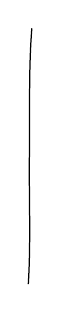
\begin{tikzpicture}[x=1cm,y=1cm]
\draw[line width=0.45pt] (0.045,3.25)
  .. controls (0.005,2.76) and (0.020,2.23) .. (0.015,1.70)
  .. controls (0.005,1.18) and (0.035,0.57) .. (0,0);
\end{tikzpicture}}

\mspage{303}

\scanpage{305}
Nous allons expliciter une relation de
compatibilité pour $S\Gamma$ relatif à un $\pi$
à \unsure{lacets}, en fixant un $i\in I=\unsure{\mathcal I(\pi)}$,
d'où un stabilisateur $\Gamma_i\subset\Gamma$ dont l'image
inverse $(S\Gamma)_i$ dans $S\Gamma$ est donc une
extension de $\Gamma_i$ par $T^I$. Utilisant la
projection $T^I\xrightarrow{\mathrm{pr}_i}T$, on trouve une
extension de $\Gamma_i$ par $T$, qu'on va décrire
d'une autre façon. L'extension $S\Gamma$
est définie intrinsèquement par la
donnée de $I$ \unsure{réalisations} \inserted{$(\pi_i)_{i\in I}$} \unsure{du groupe}
\unsure{extérieur} $\pi$ par des groupes, avec dans
chaque $\pi_i$ un $L_i\subset\pi_i$ de la classe $i$
(c'est cela, la donnée d'un système des
$(\widetilde D_i^*)$ !). Pour un autom. ext. \deleted{\unsure{$u$}} \inserted{à lacets $u\in\Gamma$} de $\pi$,
\deleted{ses ``\illegible{1}'' sont les}
pour $\forall i$ il \deleted{\unsure{y a des façons}} \inserted{est possible} de le
\unsure{réaliser} par $u_i\in\operatorname{Aut}_{\unsure{\mathrm{lac}|\mathrm{loc}}}(\pi_i)$, avec $u_i(L_i)\subset L_i$
--- cet $u_i$ est déterminé \unsure{mod} multiplication
à droite par un $\operatorname{int}(\unsure{k_i|\kappa_i}(\alpha))$, où $\alpha\in T$.
Bien entendu, $S\Gamma$ est le \unsure{ss-groupe} \unsure{des|du}
\mspage{304}

\scanpage{306}
\mspage{154}
$\displaystyle\prod_{i\in I}\operatorname{Aut}_{\unsure{\mathrm{lac}|\mathrm{loc}}}(\pi_i)$,
\deleted{\unsure{formé de} \illegible{1}} \inserted{\unsure{l'image inverse}} de la diagonale
dans l'hom. naturel de ce produit dans
$\operatorname{Autext}_{\unsure{\mathrm{lac}|\mathrm{loc}}}(\pi)^I$, \deleted{\unsure{d'où une}} \inserted{\unsure{qui est bien}} extension de
\unsure{ladite} diagonale (identifiée à $\Gamma$) par $T^I$.
Si on regarde la sous-extension \deleted{de $\Gamma_i$} obtenue
par restriction à $\Gamma_i$, on voit que la
projection $T^I\unsure{\xrightarrow{\mathrm{pr}_i}}T$ est stable par $\Gamma_i$; donc
on en déduit une extension de $\Gamma_i$ par $T$,
qui n'est autre que le groupe des
autom. \inserted{à lacets} de $\pi_i$ qui normalisent $L_i$
--- qui est bien une extension de $\Gamma_i$ par $L_i$
(\unsure{car} intersection avec $\pi_i\subset\operatorname{Aut}_{\unsure{\mathrm{lac}|\mathrm{loc}}}(\pi_i)$ \unsure{est|étant}
réduite à $L_i$).

Ceci nous montre que l'extension
de $\Gamma$ par $T^I$ a une nette tendance à
ne pas être triviale, car il en est \unsure{ainsi}
\inserted{(pour $i\in I$ fixé)} de l'extension de $\Gamma_i$ par $T$ \inserted{à} qui elle donne
naissance. Si p.ex. on a un ss-groupe
\uline{fini} $G\subset\Gamma_i^+$, l'extension induite n'est
jamais triviale si $G\ne1$, on l'a vu. En
fait, $G$ doit être cyclique et son image inverse
dans l'ext. en question est $\simeq T$\ldots
\mspage{305}

\scanpage{307}
\mspage{155}
$25^{\mathrm{bis}}$. Cas des deux groupes. Retour sur les \unsure{notations}

On se place \inserted{d'abord} pour fixer les idées dans le cas
topologique et discret, mais la motivation est
le cas d'une courbe algébrique $U$ sur un
corps de type fini $K$, où on a à la fois
le groupe $G_K=\operatorname{Aut}_K(U)$ et $\Gamma=\operatorname{Gal}(\overline K/K)$
\margin{Cas anabélien donc \unsure{$G$|$G_K$} fini}
qui \unsure{opèrent} extérieurement sur le $\pi_1(U_{\overline K})$.
Dans ce cas, $G$ et $\Gamma$ commutent, mais
on peut regarder plus généralement le cas
du groupe (plus gros que $G_K$) $G_{\overline K}=\operatorname{Aut}_{\overline K}(U)$,
sur lequel $\Gamma$ opère (de façon pas néc. triviale
--- cette opération décrit \unsure{un} groupe algébrique
étale fini sur $K$.

Supposons donc qu'on ait une surface
$U$ (orientable, $U=X-S$, $X$ \unsure{compact} \inserted{\unsure{connexe}}, $S$ fini)
sur \unsure{laquelle|la quelle} \unsure{opèrent} deux groupes $G$, $\Gamma$,
l'action de $\Gamma$ normalisant celle de $G$
--- donc on a un groupe $\mathcal G=\Gamma . G$ (produit
semi-direct, pour une certaine action de $\Gamma$
sur $G$) qui opère sur $U$. On suppose $G$
fini, mais pas néc. $\Gamma$ fini.
\mspage{306}

\scanpage{308}

On suppose choisi un rev. universel $\widetilde U$ de $U$, d'où un groupe à \unsure{lcts} $\pi=\operatorname{Aut}(\widetilde U)$, sur lequel $\mathcal G$ opère extérieurement, d'où extension
\[
(1)\qquad 1\longrightarrow\pi\longrightarrow\unsure{\mathcal E|\varepsilon}\longrightarrow\mathcal G\longrightarrow 1
\]
\margin{On va \unsure{supposer} l'action de $\mathcal G$ fidèle}
Si l'action de $\mathcal G$ sur $U$ \inserted{mod isotopie} est fidèle,
alors $\mathcal G\hookrightarrow\operatorname{Autext}(\pi)$, et l'extension précédente est l'image inverse de l'extension de Teichmüller de $\pi$
\[
1\longrightarrow\pi\longrightarrow\operatorname{Aut}_{\mathrm{lac}}(\pi)\longrightarrow\operatorname{Autext}_{\mathrm{lac}}(\pi)\longrightarrow 1.
\]

\deleted{\unsure{Soit}} On aura à regarder d'autres \unsure{rev\textsuperscript{ts}} univ. que $\widetilde U$, et leurs iso. avec $\widetilde U$.
Quand $\widetilde U=\widetilde U(P)$ est le rev. universel basé en un certain $P\in U$, alors pour des rev. universels \inserted{$\unsure{U(Q)}$} basés en \deleted{\illegible{1}} \inserted{un} \unsure{point\deleted{s}|points},
les \inserted{$U$-}iso. $\widetilde U(P)\xrightarrow{\sim}\unsure{\overline U(Q)|\widetilde U(Q)}$ correspondent \unsure{donc} aux classes de chemins de $P$ à $Q$.

Soit \deleted{\illegible{1}} $Q\in U$ tel que son groupe d'isotropie \inserted{$G_Q$} \deleted{\illegible{1}} \uline{dans $G$} soit \unsure{tel.} que $G_Q^+\ne1$.
(Donc $G_Q^+$ est cyclique). Choisissant une
\mspage{307}

\scanpage{309}
\mspage{156}

classe de chemins \inserted{$\lambda$} de $P$ à $Q$, identifiant $\unsure{\overline U(P)|\widetilde U(P)}$ à $\unsure{\overline U(Q)|\widetilde U(Q)}$, on trouve une opération de $G_Q$ sur $\widetilde U(P)$ i.e. un relèvement $G_Q\xrightarrow{r_{G_Q}}\unsure{\mathcal E|\varepsilon}$ dans l'extension (1) --- le changement de classe de chemins \inserted{de $\lambda$ en $\lambda'$} donnera un relèvement $r'_{G_Q}$ qui \deleted{\unsure{est}} sera conjugué de $r$ par un unique élément de $\pi$ \inserted{$=\pi_1(U,P)$} (l'unicité provient de $\pi^{G_Q}=\{1\}$), \unsure{savoir} celui qui fait \unsure{passer} d'un chemin à un autre.

Considérons le stabilisateur $\Gamma_Q$ de $Q$ dans $\Gamma$, \deleted{\illegible{2}} qui opère bien sûr sur $\widetilde U(Q)$ tout comme $G_Q$ (en fait c'est $\mathcal G_Q$ qui opère \inserted{d'où $r:\mathcal G_Q\to\unsure{\mathcal E|\varepsilon}$} \unsure{\dots}), donc via $\lambda$ on a aussi un \unsure{relèv\textsuperscript{t}|relèvg.} $r_{\Gamma_Q}:\Gamma_Q\longrightarrow\unsure{\mathcal E|\varepsilon}$, qui \inserted{a} $\overline{\mathrm m}$ la \unsure{propté} de \unsure{normaliser} $r_{G_Q}$ (\unsure{i.e.} op. de \deleted{\illegible{1}} $\Gamma_Q$ dessus, qui est celle provenant de l'op. donnée de $\Gamma$ sur $G$).
\margin{\uline{NB} Comme l'ens \deleted{\illegible{1}} \unsure{des} pts $Q$ est fini, et que $\mathcal G$ opère dessus, l'orbite de $Q$ sous $\mathcal G$ est finie, i.e. $\mathcal G_Q$ d'indice fini dans $\mathcal G$. et de $\overline{\mathrm m}$ $\Gamma_Q$ dans $\Gamma$.}
Pour simplifier, supposons quand $\overline{\mathrm m}$ que $\Gamma$ opère \unsure{trivial\textsuperscript{t}} sur $G$ i.e. $\mathcal G=\Gamma\times G$, alors $r_{\Gamma_Q}(\Gamma_Q)\subset\unsure{\mathcal E|\varepsilon}$ est contenu dans le \uline{centralisateur} de \inserted{$r$ (ou de} $\unsure{r_{G_Q}}(G_Q)$),
\mspage{308}

\scanpage{310}

et comme $\pi^{r(G_Q)}=1$, donc l'hom
\[
\operatorname{Centr}(r_{\deleted{\unsure{G_Q}}}(G_Q))\longrightarrow\mathcal G
\]
est injectif, le relèvement en question \inserted{$\unsure{r_{\Gamma_Q}}$} est uniquement déterminé par la condition précédente.
\margin{\uline{NB} \unsure{Indépend\textsuperscript{mt}|Indépendamment} de \unsure{tte|l'} hyp. que $\Gamma$ centralise $G$, le normalisateur de $r(G_Q)$ dans $\pi$, égal à son ``centralisateur'', est réduit à $1$, donc $\operatorname{Norm}(r(G_Q))\longrightarrow\mathcal G$ est injectif}

En fait, l'image de $\operatorname{Centr}(r(G_Q))$ dans $\mathcal G$ contient $\mathcal G_Q$, \inserted{\unsure{et}} \deleted{\illegible{5}} \unsure{$\overline{\mathrm m}$} le relèvement $\mathcal G_Q\xrightarrow{r_{\mathcal G_Q}}\unsure{\mathcal E|\varepsilon}$.
\deleted{si $\mathcal G$ est fini}
\unsure{La|Le} chose \unsure{intéressante}, c'est que \unsure{les|le} \inserted{choix d'un} relèvement\deleted{\unsure{s}} \unsure{du|des} (petit) groupe $G_Q$, impose déjà le choix d'un relèvement \unsure{du|des} (grand) groupe $\Gamma_Q$, ou $\mathcal G_Q$.

\deleted{Quand $\mathcal G$ est lui-$\overline{\mathrm m}$ fini,} je dis que l'image dans $\mathcal G$ du centralisateur \inserted{(et $\overline{\mathrm m}$ du normalisateur)} de $r(G_Q)$ est $\mathcal G_Q$ lui-$\overline{\mathrm m}$ (a priori il le contient).
\unsure{Revenant|Revenons} à $\widetilde U(Q)$ lui-$\overline{\mathrm m}$, cela signifie que \deleted{\illegible{1}} si $g\in\mathcal G$ est tel qu'il existe un autom $\widetilde g$ de $\widetilde U(Q)$ qui relève $g$, en \deleted{\unsure{commutant}} \inserted{normalisant} \deleted{\unsure{à}} \inserted{l'action de} $G_Q$, alors $g\in\mathcal G_Q$ \inserted{(et $\widetilde g$ est le relèvement évident)}. En effet, si $\widetilde g$ \deleted{\unsure{commute}} \inserted{normalise} \inserted{l'action de} $G_Q$, il \unsure{invarie|envoie} l'ens des pts fixes de $G_Q$ dans $\widetilde U(Q)$, qui est réduit \deleted{\illegible{1}} \inserted{\unsure{au point}} $\unsure{\widetilde Q|\overline Q}$
\mspage{309}
\scanpage{311}
\mspage{157}

L'ens. $\unsure{\widetilde U|U}^{!}$ des pts $Q\in U$ tels que $G_Q^+\ne(1)$ est stable par l'action de $\mathcal G$, et s'identifie (avec cette action) à \unsure{l'ens.} des relèvements \inserted{maximaux} mod $\pi$ de ss-groupes (cycliques) $\ne1$ de $G^{+}_{\deleted{\unsure{Q}}}$. Quand on connaît, pour un relèvement partiel $r$ d'un $G_Q$ dans $\mathcal E$ quel est son centralisateur dans $\mathcal E$ i.e. le relèvement correspondant de $\mathcal G_Q$, \unsure{bien|lors} de $=$ pour les conjugués de $r$ par n'importe quel \unsure{élt} $g$ (non seulement de $\pi$, mais $=$ de $\mathcal E$), par simple conjugaison.

Donc les cas à déterminer correspondent pratiquement aux orbites de $\mathcal G$ dans $U^{!}$.

On peut s'intéresser à décrire $\mathcal G$ ou $\Gamma$ en tant que ss-groupe de $\mathrm{Aut\,ext}_{\mathrm{lac}}(\pi)=\Gamma'$ \inserted{donnant lieu à l'ext. $\mathcal E'$ de $\Gamma'$ par $\pi$ (donc $\mathcal E\subset\mathcal E'$).} Mais pour tt relèvement $r$ d'un $G_Q$, considérons $\mathrm{Centr}_{\mathcal E'}(r)$, \deleted{\illegible{1}} . \unsure{on aura|on a encore} $\mathrm{Centr}_{\mathcal E'}(r)\cap\pi=(1)$ i.e. \inserted{on trouve une section au dessus de} l'image de ce centralisateur dans $\Gamma'$, soit $\Gamma'(Q)$. Cette image ne dépend que de $Q$ i.e. de la classe de $\pi$-conjugaison de $r$ ou de $r(\unsure{G_Q})$, et est remplacée par un $G$-conjugué quand $Q$ est remplacé par un $G$-conjugué. Ceci

\mspage{310}

\scanpage{312}

dit, l'intersection \inserted{$\Gamma'^{\natural}$} des $\Gamma'(Q)$, pour $Q\in U^{!}$, est un ss-groupe de $\Gamma'$ qui contient l'intersection \deleted{\unsure{de}} $\mathcal G^{\natural}$ des $\mathcal G_Q^{\deleted{\unsure{\natural}}}$, et le centralisateur de $G$ dans $\Gamma'^{\natural}$ contient de $=$ l'intersection \deleted{de} $\Gamma^{\natural}$ des $\Gamma_Q$, qui est un ss-groupe \inserted{invariant} d'indice fini de $\Gamma$. Et on peut alors se proposer s'il est possible de caractériser au moins \unsure{le|un} ss-groupe fini $\Gamma^{\natural}$ de $\Gamma$ comme $\mathrm{Centr}_{\Gamma'^{\natural}}(G)$, et \unsure{d'en récupérer} peut être $\Gamma$ comme le normalisateur de $\Gamma^{\natural}$ dans \deleted{le centralisateur} $\mathrm{Centr}_{G}(\Gamma)$.

Je m'intéresse plus particulièrement à la variante profinie de ceci, dans le cas où $U=\mathbb P^1_{\mathbb Q}\setminus\{0,1,\infty\}$, $G=\mathfrak S_3$, $\Gamma={}$ groupe de Galois de $\overline{\mathbb Q}/\mathbb Q$, \deleted{tandis} \inserted{$\unsure{P|\rho}=\exp(2i\pi/6)$}.
\margin{clôture alg. dans $\mathbb C$}

Je n'ai pas vérifié que $\Gamma\longrightarrow\mathrm{Autext}_{\mathrm{lac}}(\widehat\pi)$ soit injectif, cela n'empêche de faire des calculs dans $\mathrm{Aut}_{\mathrm{lac}}(\widehat\pi)$, fussent-ils heuristiques pour le moment.

\mspage{311}

\scanpage{313}
\mspage{158}

Je bute à des ennuis de notations -- trop de groupes sont \unsure{\uline{désignés}} par la lettre $\Gamma$ (avec évt. des primes, indices, exposants \ldots). Il y a trois types de groupes qui interviennent dans mes réflexions :

a) les groupes de Teichmüller et ses variantes, qui jouent le rôle \unsure{des|de} groupes ``universels'' opérant (\inserted{éventuellement} mod isotopie) sur des surfaces, ou sur des groupes \deleted{\unsure{à lacets}} extérieurs à lacets. Ces groupes ont tendance à être infinis

b) Des groupes (le plus souvent finis) opérant sur des surfaces topologiques, ou sur des courbes algébriques géométriques (\unsure{sans}, dans ce cas-là, bouger le corps de base).

\margin{Les cas b) et c) se mélangent parfois (dans \unsure{un} \unsure{$G$} \unsure{groupes} $\mathcal G$ ext. d'un groupe de Galois $\Gamma$ par un groupe fini \unsure{$G$}) \unsure{dans le cas de} \unsure{$G$} \unsure{Géom.} Alg.}

c) Des groupes de Galois profinis (donc infinis), surtout des corps de type fini sur $\mathbb Q$, opérant ``arithmétiquement'' sur des surfaces et leurs $\widehat{\pi}_1$ géométriques.

C'est à cause des analogies profondes entre les cas b) et c), et leurs relations étroites avec le cas a), que j'avais été induit à adopter des notations communes, mais

\mspage{312}

\scanpage{314}

qui à la longue finissent par aboutir à des collisions. Il y a donc lieu de revoir les notations. Je vais réserver la lettre $G$ \inserted{et variantes} pour des actions géométriques (cas b)) de groupes, le plus souvent finis, la lettre $\Gamma$ \inserted{et variantes} pour des groupes de Galois, la lettre $\mathcal G$ pour des groupes mixtes.

Quand aux groupes ``universels'' de type Teichmüller, comme ceux notés $\Gamma_{g,\nu}$ précédemment, je vais plutôt les noter \inserted{$\mathcal T$,} $\mathcal T_{g,\nu}$ (initiale de ``Teichmüller'', alors que $\Gamma$, \inserted{$G$} \unsure{sont} l'initiale de Galois).

Le groupe de Galois \inserted{sur $\mathbb Q$} de la clôture algébrique $\overline{\mathbb Q}$ de $\mathbb Q$ dans $\mathbb C$ \deleted{\unsure{de $\overline{\mathbb Q}$ sur}} \unsure{mérite} une lettre spéciale, je le noterai $\boldsymbol{\Gamma}$. Le quotient \deleted{\unsure{par} $\widehat{\Gamma}_{g,\nu}$ de} $\operatorname{Norm}_{\widehat{\widehat{\mathcal T}}_{g,\nu}}(\widehat{\mathcal T}_{g,\nu})/\widehat{\mathcal T}_{g,\nu}$, qui s'apparente plus à un groupe de Galois qu'à un groupe de Teichmüller, sera noté $\boldsymbol{\Gamma}_{g,\nu}$ (lettre grasse !). Dans le

\mspage{313}

\scanpage{315}
\mspage{159}

cas $(g,\nu)=(0,3)$ qui m'occupe plus particulièrement, $\boldsymbol{\Gamma}_{0,3}$ s'identifie au \deleted{\unsure{normalisateur}} \inserted{centralisateur} de $G=\mathfrak S_3$ \inserted{$=\mathcal T_{0,3}^{+}$} dans $\widehat{\widehat{\mathcal T}}_{0,3}$ -- il est contenu dans $\widehat{\widehat{\mathcal T}}_{03}^{!}$, \inserted{et peut-être égal.} On a un hom canonique
\margin{$\widehat{\widehat{\mathcal T}}$ est ici produit $\frac{1}{2}$ direct de $\mathfrak S_3=\mathcal T^+$ par $\mathcal T^{!}$}
\[
\boldsymbol{\Gamma}\longrightarrow\boldsymbol{\Gamma}_{03}
\qquad (\text{plus généralement }\boldsymbol{\Gamma}\longrightarrow\boldsymbol{\Gamma}_{g,\nu})
\]
dont j'ignore pour l'instant s'il est injectif, et encore plus s'il est surjectif. Les réflexions qui précèdent suggèrent des conditions sur l'image, qui sont surtout intéressantes si on admet les relations
\[
\widehat{\pi}^{\rho}=\widehat{\pi}^{\sigma_0}=(1)
\]

On \inserted{a} \unsure{désigné\deleted{ra}} par $\mathcal E_{g\nu}$ l'extension canonique de $\mathcal T_{g,\nu}$ par $\pi_{g,\nu}$ (qui pour $(g,\nu)$ anabélien s'identifie à $\mathcal T'_{g,\nu+1}$).

L'opération extérieure d'un groupe $G$, $\Gamma$ ou $\mathcal G$ définit aussi une extension par $\pi$ (ou par $\widehat{\pi}$), qu'on a également \unsure{désigné|désignée} par la lettre $\mathcal E$ (initiale d'extension) -- il y a à nouveau collision de notations.

\mspage{314}

\scanpage{316}

Je vais prendre la lettre $\mathfrak{S}$ (qui fait pendant à $\mathcal{T}$) pour ces extensions dans les cas universels à la Teichmüller, (en écrivant $\mathfrak{S}_{g,\nu}$ au lieu des $\Gamma'_{g,\nu+1}$, puisque l'optique est différente\ldots), et en gardant la lettre $\mathcal{E}$ dans \unsure{les|le} cas \unsure{précédents|précédent}. Donc $\mathcal{E}$ a tendance à être une sous-extension d'une $\mathfrak{S}$.

Admettant que $\boldsymbol{\Gamma}\longrightarrow\boldsymbol{\Gamma}_{0,3}$ est injectif, on aurait donc

\diagram{\begin{tikzcd}[ampersand replacement=\&,column sep=small,row sep=large]
1 \arrow[r,no head] \& \widehat{\pi}_{0,3} \arrow[r] \arrow[d,equal] \& \widehat{\widehat{\mathfrak{S}}}_{0,3} \arrow[r] \arrow[d] \& \widehat{\widehat{\mathcal{T}}}_{0,3} \arrow[r] \arrow[d] \& 1 \\
1 \arrow[r,no head] \& \widehat{\pi}_{0,3} \arrow[r] \arrow[d,equal] \& \widehat{\widehat{\mathfrak{S}}}'_{0,3} \arrow[r] \arrow[d] \& \underbrace{\unsure{\mathcal{T}^{+}_{0,3}}}_{\mathfrak{S}_{3}}\;\deleted{\unsure{\boldsymbol{\Gamma}}}\!\times\boldsymbol{\Gamma}_{0,3} \arrow[r] \arrow[d] \& 1 \\
1 \arrow[r] \& \widehat{\pi}_{03} \arrow[r] \arrow[d] \& \mathcal{E} \arrow[r] \arrow[d] \& \mathfrak{S}_{3}\times\boldsymbol{\Gamma} \arrow[r,no head] \arrow[d] \& 1 \\
1 \arrow[r] \& \pi_{0,3} \arrow[r] \& \mathfrak{S}_{03} \arrow[r,no head] \& \underbrace{\mathfrak{S}_{3}\times\unsure{\mathbb{Z}/2}}_{\mathcal{T}_{0,3}} \arrow[r] \& 1
\end{tikzcd}}

\margin{NB On note $\widehat{\widehat{\mathfrak{S}}}'_{g,\nu}$ le normalisateur de $\widehat{\mathfrak{S}}^{+}_{g,\nu}$ dans $\widehat{\widehat{\mathfrak{S}}}_{g,\nu}$, extension de $\boldsymbol{\Gamma}_{g,\nu}$ par $\widehat{\mathfrak{S}}^{+}_{g,\nu}$}

\unsure{Si|Soit} $\gamma\in\boldsymbol{\Gamma}_{0,3}$, \deleted{\unsure{qui soit}}\inserted{pour qu'il soit} dans l'image de $\boldsymbol{\Gamma}$ \deleted{\unsure{ait|est} la propriété}\inserted{il faut} \unsure{qu'il|qu'ils} \unsure{admette|admettent} un relèvement $u$ qui commute à $\rho$, et un rel. qui commute à $\sigma_{0}$ \unsure{(ce|Ce} qui, \unsure{dès|des} que $\gamma\in\widehat{\widehat{\mathcal{T}}}_{0,3}$, implique

\mspage{315}

\scanpage{317}
\mspage{160}

déjà que $\gamma$ dans $\widehat{\widehat{\mathcal{T}}}_{0,3}$ commute à $\mathcal{T}^{+}_{0,3}=\mathfrak{S}_{3}$, \deleted{donc} i.e. qu'ils est dans $\boldsymbol{\Gamma}_{0,3}$). Il se pourrait que \unsure{tout} élément de $\boldsymbol{\Gamma}_{0,3}$ ait déjà cette propriété, donc que cette condition ne \unsure{pose|fasse} pas de restriction véritable sur l'image de $\boldsymbol{\Gamma}$ dans $\boldsymbol{\Gamma}_{0,3}$.

\mspage{316}

\scanpage{318}
\mspage{161}

\uline{26} Groupes de Teichmüller profinis.

\margin{Discrétifications et prédiscrétifications.}

Soit $\pi$ un groupe profini à lacets \inserted{de type $g,\nu$}, $T$ le $\widehat{\mathbb Z}$-module inversible de ses orientations.

On suppose qu'on est dans le cas \unsure{anabélien}, et on admettra \unsure{qu'alors}
\[
\operatorname{Centre}(\pi)=\{1\}
\tag{1}
\]
plus généralement que le centralisateur dans $\pi$ de tout sous-groupe ouvert de $\pi$ est réduit à $\{1\}$. On aura donc encore une suite exacte canonique de groupes profinis
\[
1 \unsure{\longrightarrow|{-}} \pi \longrightarrow \operatorname{Aut}_{\mathrm{lac}}(\pi) \longrightarrow \operatorname{Autext}_{\mathrm{lac}}(\pi) \longrightarrow 1
\tag{\unsure{2}}
\]
On posera aussi \deleted{\unsure{$\operatorname{Autext}$}}
\[
\operatorname{Autext}_{\mathrm{lac}}(\pi)=\widehat{\widehat{\mathcal T}}(\pi)
\tag{3}
\]
\unsure{on|et} l'appellera le \uline{groupe de Teichmüller étendu} de $\pi$. On posera aussi $\widehat{\widehat{\mathfrak S}}(\pi)=\operatorname{Aut}_{\mathrm{lac}}(\pi)$, de sorte qu'on peut écrire (2) comme
\[
1 \longrightarrow \pi \longrightarrow \widehat{\widehat{\mathfrak S}}(\pi) \longrightarrow \widehat{\widehat{\mathcal T}}(\pi) \longrightarrow 1
\tag{2'}
\]

Appelons "base" de $\pi$ un \unsure{ens} d'\unsure{élts} de $\pi$ $(x_i,y_i)_{1\leq i\leq g}$, $(\ell_j)_{1\leq j\leq\nu}$, \inserted{les $\ell_j$ \unsure{engend$^{\mathrm t}$} les diff. groupes à lacets} satisfaisant
\[
\deleted{\unsure{\prod_i}\,\unsure{[x_i,y_i]}\,\unsure{\cdots[x_g,y_g]\ell_1}}
\quad
\inserted{\ell_\nu\ell_{\nu-1}\cdots\ell_1[x_g,y_g]\cdots[x_1,y_1]=1}
\tag{\unsure{4}}
\]
et tels que ceci soit une relation génératrice.

\mspage{317}

\scanpage{319}

\margin{ou encore, on définit $\Pi_{g,\nu}$ comme le groupe discret \unsure{de|des} gén. les $x_i,y_i,\ell_j$ et de relation de \unsure{définition} (4)}

\unsure{Si} on choisit dans $\Pi_{g,\nu}$ une base (discrète) (\unsure{définition|Définition} correspondante), \unsure{d'où} une base de $\widehat{\Pi}_{g,\nu}$, on aura une bijection évidente
\[
\operatorname{Bases}(\pi) \xleftarrow{\sim} \operatorname{Isom}_{\mathrm{lac}}(\widehat{\Pi}_{g,\nu},\pi)
\tag{5}
\]

L'ensemble des bases de $\pi$ est un ensemble homogène \unsure{dans|sous} \deleted{\illegible{1}} $\widehat{\widehat{\mathfrak S}}(\pi)=\operatorname{Aut}_{\mathrm{lac}}(\pi)$. \unsure{Soit|Si} la \deleted{\unsure{$\Pi_0$ d}} base correspond à un iso $u:\widehat{\Pi}_{g,\nu}\longrightarrow\pi$, le groupe \inserted{$\Pi_0$} engendré par les $x_i,y_i,\ell_j$ n'est autre que $\deleted{\unsure{\Pi_0}}\inserted{u}(\Pi_{g,\nu})$. \deleted{Une des} \inserted{les ss-groupes} de $\pi$ qui peuvent s'obtenir ainsi sont appelés les \uline{discrétifications} de $\pi$. Celles-ci forment un ensemble homogène sous $\widehat{\widehat{\mathfrak S}}=\operatorname{Aut}_{\mathrm{lac}}(\pi)$, \inserted{can.} isomorphe au quotient du $\widehat{\widehat{\mathfrak S}}_{g,\nu}$-\deleted{\unsure{torseur}}\inserted{ensemble} à droite $\operatorname{Isom}_{\mathrm{lac}}(\widehat{\Pi}_{g,\nu},\pi)$ par $\mathfrak S_{g,\nu}$ :
\[
\operatorname{Discrt}(\pi) \xleftarrow{\sim} \operatorname{Isom}_{\mathrm{lac}}(\widehat{\Pi}_{g,\nu},\pi)/\mathfrak S_{g,\nu}
\tag{6}
\]
Les \unsure{autom} \inserted{(profinis à lacets)} de $\pi$ fixant \inserted{une discrétification} $\Pi_0$ s'identifient aux \unsure{autom} du groupe discret \inserted{à lacets} $\Pi_0$.
\[
\operatorname{Aut}_{\mathrm{lac}}(\pi,\Pi_0)\simeq\operatorname{Aut}_{\mathrm{lac}}(\Pi_0)
\tag{7}
\]

\mspage{318}

\scanpage{320}
\mspage{162}

La bijection (5) met sur l'ens des Bases de $\pi$ une structure de bitorseur sous $\widehat{\widehat{\mathfrak S}}(\pi),\widehat{\widehat{\mathfrak S}}_{g,\nu}$, et \unsure{les|la} \unsure{topologies|topologie} \unsure{correspondantes|correspondante} en fait un ens profini. L'ensemble des discrétifications de $\pi$, qui est un quotient de l'ens précédent, hérite d'une topologie quotient, qui n'est autre que la top. quotient du deuxième membre de (6). \deleted{Sauf dans les cas \unsure{exceptionnels} \unsure{$(g,\nu)=(0,3)$} \unsure{où} $\mathfrak S_{g,\nu}$} \inserted{Cet espace n'est} pas séparé \inserted{(NB $\mathfrak S_{g,\nu}$ est \unsure{tjs} infini)}, car le groupe $\mathfrak S_{g,\nu}\subset\widehat{\widehat{\mathfrak S}}_{g,\nu}$ n'est pas fermé. On désigne par $\unsure{\widetilde{\operatorname{Discrt}}'|\operatorname{Discrt}'}(\pi)$ l'espace topologique séparé associé, s'identifiant à $\operatorname{Isom}_{\mathrm{lac}}(\widehat{\Pi}_{g,\nu},\pi)/\unsure{\overline{\mathfrak S}}_{g,\nu}$, où $\overline{\mathfrak S}_{g,\nu}$ désigne l'adhérence de $\mathfrak S_{g,\nu}$ dans $\widehat{\widehat{\mathfrak S}}_{g,\nu}$. On a d'ailleurs un hom surjectif évident $\widehat{\mathfrak S}_{g,\nu}\longrightarrow\unsure{\widehat{\widehat{\mathfrak S}}|\overline{\mathfrak S}}_{g,\nu}$ dont l'image est $\overline{\mathfrak S}_{g,\nu}$, \unsure{nous admettrons} qu'il est injectif, et identifierons $\overline{\mathfrak S}_{g,\nu}$ à $\widehat{\mathfrak S}_{g,\nu}$. Ainsi
\[
\operatorname{Discrt}'(\pi)\simeq\operatorname{Isom}_{\mathrm{lac}}(\widehat{\Pi}_{g,\nu},\pi)/\widehat{\mathfrak S}_{g,\nu}
\tag{\unsure{8}}
\]

\mspage{319}
\scanpage{321}

\unsure{Un} élément de $\operatorname{Discr\acute{e}t}^{\unsure{\prime}}(\pi)$ s'appelle une
classe de discrétifications de $\pi$\inserted{\unsure{ou} \unsure{pré-discrétification} de $\pi$}.
Si $\pi_0$ est une discrétification, on désigne sa classe par
$\pi_0^{\unsure{\natural}}$. L'ens. des classes de discrétifications sur $\pi$
est un \unsure{espace} hom. $\widehat{\widehat{\unsure{\mathfrak{S}|\mathcal{G}}}}(\pi)$, le stabilisateur
de $\pi_0^{\unsure{\natural}}$ \unsure{s'identifie à|s'identifiant} : l'adhérence de
$\unsure{\mathfrak{S}|\mathcal{G}}(\pi_0)=\operatorname{Aut}_{\mathrm{lac}}(\pi_0)$ dans
$\widehat{\widehat{\unsure{\mathfrak{S}|\mathcal{G}}}}(\pi)$, ou encore :
$\widehat{\unsure{\mathfrak{S}|\mathcal{G}}}(\pi_0)$.
Celle-ci contient toujours $\pi$.
\[
\operatorname{Aut}_{\mathrm{lac}}(\pi,\pi_0^{\unsure{\natural}})
\simeq\widehat{\unsure{\mathfrak{S}|\mathcal{G}}}(\pi_0)
\]

\deleted{On a} pour tte discrétification $\pi_0^{\unsure{\natural}}$, le sous-groupe de
$\widehat{\widehat{\unsure{\mathfrak{S}|\mathcal{G}}}}(\pi)$ des \unsure{autom.} à lacets qui fixent
$\pi_0^{\unsure{\natural}}$ est noté $\widehat{\unsure{\mathfrak{S}|\mathcal{G}}}(\pi_0^{\unsure{\natural}})$,
c'est donc l'image inverse d'un ss-groupe de
$\widehat{\widehat{\mathcal{T}}}(\pi)$, noté
$\widehat{\mathcal{T}}(\pi_0^{\unsure{\natural}})$. On a donc une inclusion de
structures d'extensions

(10)
\diagram{\begin{tikzcd}[ampersand replacement=\&]
1 \arrow[r] \& \pi \arrow[r] \&
\widehat{\unsure{\mathfrak{S}|\mathcal{G}}}(\pi_0^{\unsure{\natural}}) \arrow[r] \arrow[d,hook] \&
\widehat{\mathcal{T}}(\pi_0^{\unsure{\natural}}) \arrow[r] \arrow[d,hook] \& 1 \\
1 \arrow[r] \& \pi \arrow[r] \&
\widehat{\widehat{\unsure{\mathfrak{S}|\mathcal{G}}}}(\pi) \arrow[r] \&
\widehat{\widehat{\mathcal{T}}}(\pi) \arrow[r] \& 1
\end{tikzcd}}

\margin{\uline{NB} L'ens des classes de discrétifications de $\pi$ se décrit
\illegible{2} du groupe \uline{ext} $\pi$, comme
$\operatorname{Isom\,ext}(\widehat{\Pi}_{g,\nu},\pi)$\deleted{\illegible{1}}
divisé par $\widehat{\mathcal{T}}_{g,\nu}$.
On a d'ailleurs \unsure{une flèche} de degré $2$
\diagram{\begin{tikzcd}[ampersand replacement=\&]
\operatorname{Isom\,ext}(\widehat{\Pi}_{g,\nu},\pi)/\widehat{\mathcal{T}}_{g,\nu}^{+}
\arrow[d] \\
\operatorname{Isom\,ext}(\widehat{\Pi}_{g,\nu},\pi)/\widehat{\mathcal{T}}_{g,\nu}
\end{tikzcd}}
ce qui permet pour \unsure{tte|les} \unsure{clas.} de discrétifications, de définir
ses deux \uline{\unsure{orientations}}, et parler des
discrétifications \uline{orientées}.}

\mspage{320}

\scanpage{322}
\mspage{163}

(On montre par voie arithmético-géométrique que l'inclusion
$\widehat{\mathcal{T}}\longrightarrow\widehat{\widehat{\mathcal{T}}}$
n'est jamais un iso.) On trouve ainsi une application
\[
\tag{11}
\operatorname{Discr\acute{e}t}^{\unsure{\prime}}(\pi)\longrightarrow
\text{Ss-groupes fermés de }\widehat{\widehat{\mathcal{T}}}(\pi)
\]
évidemment compatible à l'action de
\deleted{$\unsure{\widehat{\widehat{\mathcal{T}}}}$}
$\widehat{\widehat{\unsure{\mathfrak{S}|\mathcal{G}}}}(\pi)$ (transport de structure) -- opérant
à droite via $\widehat{\widehat{\mathcal{T}}}(\pi)$ et ses autom. int. sur lui-même.

On trouve ainsi une classe de conjugaison, bien déterminée \unsure{de|des}
ss-groupes fermés de $\widehat{\widehat{\mathcal{T}}}(\pi)$,
qu'on appelle ses sous-groupes de Teichmüller ``\uline{géométriques}''.
\deleted{Il n'est nullement improbable d'ailleurs que
$\widehat{\mathcal{T}}(\pi_0^{\unsure{\natural}})$ soit \illegible{1}}
Il se pourrait d'ailleurs que $\widehat{\mathcal{T}}_{g,\nu}$ soit
son propre normalisateur dans $\widehat{\widehat{\mathcal{T}}}_{g,\nu}$
-- équivalent à l'assertion que (11) est \unsure{injective|bijective|injection} :
La donnée d'une classe de discrétifications\inserted{de $\pi$}
serait équivalente à celle d'un ss-groupe de Teichmüller géométrique dans
\deleted{$\unsure{\widehat{\widehat{\mathcal{T}}}}$}
son groupe de Teichmüller \unsure{étendu} $\widehat{\widehat{\mathcal{T}}}$.

\margin{c'est complètement déconnant et ultra-faux
-- un moment d'égarement ! Cela apparaît clairement par la suite\ldots
La question \unsure{judicieuse} (avec laquelle \unsure{j'ai} dû
\unsure{sur le coup} confondre) \unsure{c'est} si $\widehat{\mathcal{T}}$ est
\uline{invariant} dans $\widehat{\widehat{\mathcal{T}}}$, i.e. si
le normalisateur est $\widehat{\widehat{\mathcal{T}}}$ \unsure{tt|tout} \unsure{entier} !}

\mspage{321}

\scanpage{323}

Notons qu'on a les hom canoniques
\[
\tag{12}
\widehat{\widehat{\mathcal{T}}}\deleted{\unsure{(\pi_0^{\natural})}}
\xrightarrow{\chi}\widehat{\unsure{\mathbb{Z}}}^{*}
\]
\[
\tag{13}
\widehat{\widehat{\mathcal{T}}}\longrightarrow
\unsure{\mathfrak{S}_{I}|\mathcal{G}_{I}}
\]
\margin{où $I=I(\pi)$ est \unsure{l'ens|l'ens.} des classes de conj. de ss-groupes à lacets de $\pi$}
induisant sur $\widehat{\mathcal{T}}(\pi_0^{\unsure{\natural}})$ des
\deleted{\unsure{continus}} hom correspondants -- d'où la définition des
ss groupes $\widehat{\widehat{\mathcal{T}}}^{!}$,
$\widehat{\widehat{\mathcal{T}}}^{+}$,
$\widehat{\widehat{\mathcal{T}}}^{!+}$ et de $\overline{\mathrm m}$ pour
$\widehat{\mathcal{T}}$. Noter que $\chi$ ne prend sur $\widehat{\mathcal{T}}$
que les valeurs $\pm1$.

Le sous-groupe $\widehat{\mathcal{T}}^{+}$ des autom. ext. des
\unsure{grps|groupes} à lacets profinis $\pi$,
\deleted{\illegible{2}}\inserted{fixant} une classe de discrétifications
$\pi_0^{\unsure{\natural}}$ et de multiplicateur $+1$, joue un rôle très particulier.
À l'opposé de ce \unsure{qu'on} peut conjecturer sur $\widehat{\mathcal{T}}$
(dont $\widehat{\mathcal{T}}^{+}$ est un sous-groupe \unsure{ouvert|invariant} d'indice $2$),
on supposerait plutôt que $\widehat{\mathcal{T}}^{+}$ est invariant dans
$\widehat{\widehat{\mathcal{T}}}$. En tt état de cause,
les ss-groupes ainsi définis dans $\widehat{\widehat{\mathcal{T}}}$
\deleted{qui}\inserted{via} \unsure{classes} de discrétifications de $\pi$
\deleted{\illegible{1}} (peut-être

\mspage{322}

\scanpage{324}
\mspage{164}

n'y en a-t-il qu'un seul et unique!) s'appelleront les sous-groupes de Teichmüller géométriques \uline{stricts}. Le choix d'un tel sous-groupe \inserted{de $\widehat{\widehat{\mathcal{T}}}$} est, en tt état de cause, un élément de structure \unsure{nettement} plus faible que celle d'une classe de \unsure{discrétifications}, et $\overline{\mathrm m}$ que celle d'un ss-groupe de Teichmüller géométrique (pas strict).

Pour préciser les relations entre ces deux notions, rappelons d'abord que $\widehat{\mathcal{T}}^{+}=\Sigma$ se déduit de $\widehat{\mathcal{T}}$ comme noyau de $\chi\mid\widehat{\mathcal{T}}:\widehat{\mathcal{T}}\longrightarrow\{\pm1\}$. D'autre part, \deleted{soit} (pour un ss-groupe de Teichmüller géom. strict choisi $\widehat{\mathcal{T}}^{+}$) considérons
\[
(14)\qquad
\unsure{\mathcal{N}|N}_{\Sigma}=\mathcal{N}
=\operatorname{Norm}_{\widehat{\widehat{\mathcal{T}}}}
\bigl(\deleted{\widehat{\mathcal{T}}^{+}}\inserted{\Sigma}\bigr)
\qquad (\Sigma=\widehat{\mathcal{T}}^{+})
\]
(peut-être tjrs égal à $\widehat{\widehat{\mathcal{T}}}$ tt entier)

évidemment (si $\deleted{\widehat{\mathcal{T}}^{+}}\inserted{\Sigma}$ provient d'un $\widehat{\mathcal{T}}$)
\[
(15)\qquad
\underset{\inserted{\unsure{=}\widehat{\mathcal{T}}^{+}}}
{\deleted{\widehat{\mathcal{T}}^{+}}\inserted{\Sigma}}
\subset\widehat{\mathcal{T}}\subset\mathcal{N}_{\Sigma}.
\]
\deleted{et $\mathcal{N}/\widehat{\mathcal{T}}^{+}$ est}
Le groupe profini $\mathcal{N}/\deleted{\widehat{\mathcal{T}}^{+}}\inserted{\Sigma}$
\deleted{est} associé à \deleted{la \unsure{struc}}
$\deleted{\widehat{\mathcal{T}}^{+}}\inserted{\Sigma}$ se note
$\boldsymbol{\Gamma}_{\deleted{\unsure{\widehat{\mathcal{T}}^{+}}}\inserted{\Sigma}}$
\deleted{\illegible{1}} \deleted{\illegible{2}}
(si $\deleted{\widehat{\mathcal{T}}^{+}}\inserted{\Sigma}$ est unique, on note $\boldsymbol{\Gamma}_{\pi}$);

\mspage{323}

\scanpage{325}

et les $\widehat{\mathcal{T}}\deleted{\unsure{\mathcal G}}$ \unsure{donnant} naissance au $\overline{\mathrm m}$ $\deleted{\widehat{\mathcal{T}}^{+}}\inserted{\Sigma}$ correspondent \deleted{\unsure{aux cl}} à une classe de conjugaison d'éléments d'ordre $2$ de $\boldsymbol{\Gamma}_{\deleted{\unsure{\widehat{\mathcal{T}}^{+}}}\inserted{\Sigma}}$. Il est clair \deleted{\unsure{qu'on|que}} en tous cas qu'on a une application injective
\[
(16)\qquad
\begin{gathered}
\text{ens des ss-groupes}\\
\text{de Teichmüller géom}\\
\widehat{\mathcal{T}}\text{ de }\widehat{\widehat{\mathcal{T}}}\text{ tels que}\\
\widehat{\mathcal{T}}^{+}=\Sigma
\end{gathered}
\longrightarrow
\begin{gathered}
\text{ens des }\unsure{\text{éléments}|\text{élémts}}\\
\text{d'ordre }2\text{ de }\boldsymbol{\Gamma}_{\Sigma}
\end{gathered}
\quad :
\]
et que son image est stable par conjugaison. Montrons que \unsure{deux|les} éléments de l'image sont conjugués par $\boldsymbol{\Gamma}_{\Sigma}$. En effet, soient
\[
\widehat{\mathcal{T}},\ \widehat{\mathcal{T}}^{\prime}\supset\Sigma
\quad\text{tels que}\quad
\Sigma=\widehat{\mathcal{T}}^{+}=\widehat{\mathcal{T}}^{\prime+}.
\]
\deleted{On \illegible{1} \unsure{évidemment}}
\inserted{$\exists\,g\in\widehat{\widehat{\mathcal{T}}}$}
tel que
$\widehat{\mathcal{T}}^{\prime}=\operatorname{int}(g)\unsure{\mathcal{T}}$,
et on \unsure{aura|a} donc
$\widehat{\mathcal{T}}^{\prime+}=\operatorname{int}_{g}\widehat{\mathcal{T}}^{+}$
i.e. $g\in\mathcal{N}$, OK.

Les éléments d'ordre $2$ ainsi obtenus dans $\boldsymbol{\Gamma}_{\Sigma}$ s'appellent les involutions canoniques. On en donnera une interprétation conjecturale remarquable plus bas. L'ens. $\widehat{\widehat{\mathcal{T}}}/\mathcal{N}$ s'identifie à l'ens des \unsure{ss-groupes} de

\mspage{324}

\scanpage{326}
\mspage{165}

Teichmüller géométriques stricts (une fois choisi l'élément ``origine'' $\Sigma$). Plus \unsure{intrinsèquement}, on \unsure{aura}:
\[
(17)\qquad
\begin{gathered}
\text{Ens des ss-groupes de}\\
\text{Teichm. géom stricts}\\
\text{de }\widehat{\widehat{\mathcal{T}}}(\pi)
\end{gathered}
\unsure{\xleftarrow{\sim}|\simeq}
\operatorname{Isomext}_{\unsure{\mathrm{lac}}}
(\widehat{\Pi}_{g,\nu},\pi)/\unsure{\mathcal{N}_{g,\nu}}
\]
où on pose, comme de juste
\[
(18)\qquad
\mathcal{N}_{g,\nu}
=\operatorname{Norm}_{\widehat{\widehat{\mathcal{T}}}_{g,\nu}}
\bigl(\widehat{\mathcal{T}}_{g,\nu}^{+}\bigr)
\]
(peut-être égal à $\widehat{\widehat{\mathcal{T}}}_{g,\nu}$ tt entier!)

Considérons maintenant le \uline{topos modulaire} \uline{sur} $\mathbb{Q}$ des courbes algébriques de type $(g,\nu)$, noté $M_{g,\nu\,\mathbb{Q}}$, ou simplement $M_{g,\nu}$. Si nous choisissons un rev. universel $\widetilde{M}_{g,\nu}$ de $M_{g,\nu\,\mathbb{Q}}$ (d'où un rev. universel de $\unsure{\operatorname{Spec}}\mathbb{Q}$ i.e. une clôture alg. $\overline{\mathbb{Q}}$ de $\mathbb{Q}$) on peut \unsure{préciser} le $\pi_1(M_{g,\nu\,\mathbb{Q}})$ comme le groupe des $M_{g,\nu\,\mathbb{Q}}$-\unsure{autom} de ce \unsure{revêt|revêtement}; \deleted{\unsure{et en} \unsure{faire} \illegible{1}} \inserted{l'appeler le} \uline{groupe de Teichmüller arithmétique} de type $(g,\nu)$ (relatif au choix de $\widetilde{M}_{g,\nu\,\mathbb{Q}}$). On aura donc une suite exacte

\mspage{325}

\scanpage{327}

\[
(19)\qquad 1\longrightarrow \pi_1(M_{g,\nu\,\overline{Q}})
\longrightarrow \pi_1(M_{g,\nu})
\longrightarrow \operatorname{Gal}(\overline{Q}/Q)\longrightarrow 1
\]
\deleted{\(1\longrightarrow \unsure{\widehat{\mathcal{T}}_{g,\nu}}\longrightarrow \unsure{\Gamma}\)}

(\unsure{où} $\overline{Q}$ et les pts base sont \unsure{explicités} comme il a été dit) Notons que par la théorie \unsure{transcendante} de Teichmüller, on a un iso. (défini mod \unsure{opération} \unsure{induite} par $\pi_1(M_{g,\nu})$ sur $\pi_1(M_{g,\nu,\overline{Q}})$)
\[
(20)\qquad \pi_1(\unsure{M_{g,\nu,\overline{Q}}})\simeq\widehat{\mathcal{T}}_{g,\nu}^{+}
\qquad (\text{compactifié profini de }\mathcal{T}_{g,\nu}^{+})
\]

Considérons d'autre part le \unsure{schéma.} $\unsure{U|\mathcal{U}}_{g,\nu}$\inserted{ sur $M_{g,\nu}$}, courbe de type $(g,\nu)$ ``universelle''

On a donc, en choisissant un rev. universel $\widetilde{\unsure{U|\mathcal{U}}}_{g,\nu}$ de celle-ci \uline{\unsure{en dessus}} du rev. universel choisi $\unsure{\widetilde{M}_{g,\nu}^{\natural}}$ de $M_{g,\nu}$, une suite exacte
\diagram{
\begin{tikzcd}[column sep=large,row sep=large,ampersand replacement=\&]
(21) \& 1 \arrow[r] \& \pi \arrow[r] \arrow[dd,"\Vert" description] \& \pi_1(\unsure{\overset{\deleted{\sim}}{\unsure{U|\mathcal{U}}}_{g,\nu}}) \arrow[r] \arrow[dd] \& \pi_1(M_{g,\nu}) \arrow[r] \arrow[dd] \& 1 \\
\text{qui s'envoie dans :} \& \& \& \& \& \\
(22) \& 1 \arrow[r] \& \pi \arrow[r] \& \widehat{\widehat{\unsure{\mathfrak{S}|\mathcal{G}}}}(\pi) \arrow[r] \& \widehat{\widehat{\mathcal{T}}}(\pi) \arrow[r] \& 1
\end{tikzcd}
}
et de $\overline{\mathrm m}$ pour $\unsure{U|\mathcal{U}}_{g,\nu\,\overline{Q}}\longrightarrow M_{g,\nu\,\unsure{\overline{Q}|Q}}$

\mspage{326}

\scanpage{328}
\mspage{\unsure{166|168}}

\[
\unsure{(\overline{21})|(\overline{21}')}\qquad
1\longrightarrow\pi\longrightarrow\pi_1(\unsure{U|\mathcal{U}}_{g,\nu\,\overline{Q}})
\longrightarrow\pi_1(M_{g,\nu\,\overline{Q}})\longrightarrow1
\]
\deleted{\(\unsure{(\overline{22})}\qquad 1\longrightarrow\pi\longrightarrow\)}

On a bien sur un \unsure{isom} de groupes à \unsure{lacets|bouts}
\[
(23)\qquad \pi\simeq\widehat{\Pi}_{g,\nu}
\]
dont on voudrait déterminer l'indétermination de façon précise

Notons $M_{g,\nu\,C}$ le \deleted{\illegible{1}}\inserted{topos} modulaire de Teichmüller complexe, défini à l'aide de la surface \deleted{diff.}\inserted{$C^\infty$} $\unsure{U|\mathcal{U}}_{g,\nu}$, il est muni du rev. universel canonique $\widetilde{M}_{g,\nu\,C}$ (\S~21)
\margin{$\widetilde{M}_{g,\nu\,C}=E_g/\unsure{A_{g,\nu}^{0}|A_{g,\nu}^{\circ}}$}
de groupe \unsure{d'autom.} $\mathcal{T}_{g,\nu}^{+}$ justement \unsure{--|...}
$\unsure{U|\mathcal{U}}_{g,\nu\,C}$ étant lui aussi muni d'un rev. universel \unsure{en dessus} du précédent,
$\widetilde{\unsure{U|\mathcal{U}}}_{g,\nu\,C}=E_g/\unsure{A_{g,\nu+1}^{0}|A_{g,\nu+1}^{\circ}}$.
Ceci donne naissance à la suite exacte de groupes discrets (dans le contexte topologie générale)
\diagram{
\begin{tikzcd}[column sep=large,row sep=large,ampersand replacement=\&]
(24) \& 1 \arrow[r] \& \Pi_{g,\nu} \arrow[r] \arrow[dd] \& \unsure{\mathfrak{S}|\mathcal{G}}_{g,\nu}^{+} \arrow[r] \arrow[d,equal] \& \mathcal{T}_{g,\nu}^{+} \arrow[r] \arrow[d,equal] \& 1 \\
\& \& \& \pi_1(\unsure{U|\mathcal{U}}_{g,\nu\,C}) \arrow[d] \& \pi_1(M_{g,\nu\,C}) \arrow[d] \& \\
\text{(s'envoyant dans} \& 1 \arrow[r] \& \Pi_{g,\nu} \arrow[r] \& \operatorname{Aut}_{\mathrm{lac}}\deleted{\unsure{\mathrm{ext}}}(\Pi_{g,\nu}) \arrow[r] \arrow[d,equal] \& \operatorname{Aut\,ext}_{\mathrm{lac}}(\Pi_{g,\nu}) \arrow[r] \arrow[d,equal] \& 1 \\
\& \& \& \unsure{\mathfrak{S}|\mathcal{G}}_{g,\nu} \& \mathcal{T}_{g,\nu} \&
\end{tikzcd}
}
par un \unsure{isom|hom.} de \unsure{structures} d'extensions), qui par passage aux complétés profinis donne la suite exacte analogue pour les

\mspage{327}

\scanpage{329}

multiplicités algébriques sur $\mathbb C$

\diagram{\begin{tikzcd}[ampersand replacement=\&,column sep=1.3em,row sep=1.2em]
(25) \& 1 \arrow[r] \&
\widehat{\Pi}_{g,\nu} \arrow[r] \arrow[d,equal] \&
\deleted{\unsure{\widehat{\Pi}}}\,\widehat{\mathcal G}_{g,\nu}
  \arrow[r] \arrow[d,very thick] \&
\widehat{\mathcal T}_{g,\nu}^{+} \arrow[r]
  \arrow[d,phantom,"{\rotatebox{-90}{$\unsure{\hookrightarrow}$}}" description] \& 1 \\
\& \& \inserted{\widehat{\Pi}_{g,\nu}} \arrow[r] \&
\inserted{\operatorname{Aut}\deleted{\unsure{\mathrm{ext}}}_{\mathrm{lac}}(\widehat{\Pi}_{g,\nu})}
  \arrow[r] \&
\inserted{\operatorname{Autext}_{\mathrm{lac}}(\widehat{\Pi}_{g,\nu})}
  \& \\[-0.7em]
\& \& \& |[xshift=-2.2em]| {\inserted{\raisebox{1ex}{\rotatebox[origin=c]{-60}{$=$}}\,\unsure{\widehat{\widehat{\mathcal G}}}_{g,\nu}}} \&
|[xshift=-2.2em]| {\inserted{\raisebox{1ex}{\rotatebox[origin=c]{-60}{$=$}}\,\widehat{\widehat{\mathcal T}}_{g,\nu}}} \&
\end{tikzcd}}

Cette situation \unsure{provient} d'ailleurs \unsure{canoniquement} d'une situation analogue sur $\overline{\mathbb Q}_0=\text{clôture alg de }\mathbb Q\text{ dans }\mathbb C$, le choix de $\widetilde{\unsure{U|\mathcal{U}}}_{g,\nu\mathbb C}$ définissant un $\widetilde{\unsure{U|\mathcal{U}}}_{g,\nu\overline{\mathbb Q}_0}$, d'où un $\widetilde{M}_{g,\nu\overline{\mathbb Q}_0}$.

Pour définir un isom entre cette suite (25) et la suite exacte $(\overline{21})$ \deleted{il faut} (\unsure{munie} de \unsure{$2$ homs|son hom.} dans (22)) il faut

$1^{\circ})$ choisir un isom $\overline{\mathbb Q}\simeq\overline{\mathbb Q}_0$ --- l'indétermination est dans $\mathrm{Gal}(\overline{\mathbb Q}/\mathbb Q)$ ; ce qui permet d'identifier $\overline{\mathbb Q}$ et $\overline{\mathbb Q}_0$ ;

$2^{\circ})$ Choisir un isom (\deleted{\unsure{entre}} $\overline{\mathbb Q}=\overline{\mathbb Q}_0$) de $(\widetilde{\unsure{U|\mathcal{U}}}_{g,\nu})_0$ (construit par voie \unsure{transcendante|transcendant} sur $\mathbb C$ et descendu à $\overline{\mathbb Q}_0$) avec $\widetilde{\unsure{U|\mathcal{U}}}_{g,\nu\overline{\mathbb Q}}$ --- l'indétermination est dans $\pi_1(M_{g,\nu\overline{\mathbb Q}})$.

En résumé, on a une classe d'iso de \unsure{(24)|(21)}\inserted{\unsure{2|?}} et (25), défini mod autom \inserted{\deleted{\illegible{1}} \illegible{1} \unsure{une fois choisi} $\overline{\mathbb Q}\simeq\overline{\mathbb Q}_0$} intérieurs dans \inserted{le groupe \unsure{\uline{profini}}} $\pi_1(\unsure{U|\mathcal{U}}_{g,\nu})$. (\unsure{Ces|Les} isomorphismes \inserted{\unsure{\uline{correspondants}}} transforment la \deleted{structure} \uline{classe de \unsure{discrétification}} \uline{orientée} \unsure{Standard|standard} de $\widehat{\Pi}_{g,\nu}$ en \deleted{\unsure{une classe}} \inserted{exactement} \uline{une} classe de discrétifications orientées de $\pi$.

\mspage{328}

\scanpage{330}
\mspage{167}

\deleted{Ainsi $\pi$ de (21) est \unsure{can.} muni d'une \deleted{\unsure{classe de}} \inserted{\unsure{quasi}} discrétification orientée \inserted{\unsure{$\pi_0^{\natural}$}}, et dans l'hom de $(\overline{21})$ dans (22), on trouve que $\pi_1(\unsure{U|\mathcal{U}}_{g,\nu\overline{\mathbb Q}})$ s'identifie à $\widehat{\unsure{\mathfrak{S}|\mathcal{G}}}(\unsure{\pi_0^{\natural}})$, et $\pi_1(M_{g,\nu})$ à $\widehat{\mathcal T}(\unsure{\pi_0^{\natural}})$ \unsure{$\longrightarrow$}}

Changeant le choix de l'isom en son complexe conjugué, on trouve la \inserted{\unsure{quasi-}} \unsure{discrétification} orientée opposée.

On voit d'autre part que l'image de $\pi_1(M_{g,\nu\overline{\mathbb Q}})\unsure{\subset}\pi_1(M_{g,\nu})$ dans $\widehat{\widehat{\mathcal T}}(\pi)$ n'est autre que le $\widehat{\mathcal T}^{+}$ \unsure{correspondant|correspond.} à une \inserted{quelconque} des classes de quasi-rigidifications discrètes choisies --- le sous-groupe ne dépend pas du choix de cette classe --- ce qui ne fait qu'exprimer que l'image de $\pi_1(M_{g,\nu\overline{\mathbb Q}})$ dans $\widehat{\widehat{\mathcal T}}(\pi)$, \unsure{considéré|considérée} comme sous-groupe de l'image du groupe plus grand $\pi_1(M_{g,\nu})$, y est \unsure{invariante|invariant} --- ce qui résulte du fait que $\pi_1(M_{g,\nu\overline{\mathbb Q}})$ est \unsure{invariant} dans $\pi_1(M_{g,\nu\unsure{\mathbb Q|\overline{\mathbb Q}}})$. Ainsi $\pi$

\mspage{329}
\scanpage{331}

est muni canoniquement (non d'une quasi-rigidification discrète \inserted{orientée}, ce qui dépend du choix d'un isom $\overline{\mathbb Q}\simeq\overline{\mathbb Q}_0$ i.e. d'un plongement $\overline{\mathbb Q}\subset\mathbb C$) mais du moins d'un groupe de Teichmüller géométrique strict $\Sigma\subset\widehat{\widehat{\mathcal T}}(\pi)$, à savoir l'image de $\pi_1(M_{g,\nu\overline{\mathbb Q}})$, \inserted{isomorphe à} Ceci posé, On a un hom canonique d'extensions de groupes

\diagram{(26)\quad
\begin{tikzcd}[ampersand replacement=\&, column sep=small]
1 \arrow[r] \&
\pi_1(M_{g,\nu\overline{\mathbb Q}}) \arrow[r] \arrow[d, "{\unsure{\wr|2}}"] \&
\pi_1(M_{g,\nu}) \arrow[r, no head] \arrow[d] \&
\operatorname{Gal}(\overline{\mathbb Q}/\mathbb Q) \arrow[r] \arrow[d] \&
1 \\
1 \arrow[r] \&
\Sigma \arrow[r] \&
\unsure{\mathcal N|N}_\Sigma \arrow[r] \arrow[d, equal] \&
\Gamma_\Sigma \arrow[r] \arrow[dr] \&
1 \\
\& \&
\operatorname{Norm}_{\widehat{\widehat{\mathcal T}}(\pi)}(\Sigma) \&
\&
\text{\margin{groupe des autom. \deleted{\unsure{``arithmétiques}}\inserted{extérieurs} "arithmétiques" de $\pi$ (muni de $\Sigma$)}}
\end{tikzcd}}

Pour le choix d'un isom $\overline{\mathbb Q}\simeq\overline{\mathbb Q}_0$ i.e. d'un plongement $\overline{\mathbb Q}\subset\mathbb C$, l'image de la conjugaison complexe de $\operatorname{Gal}(\overline{\mathbb Q}_0/\mathbb Q)$ n'est autre que \unsure{l'élt} d'ordre $2$ de $\Gamma_\Sigma$ associé au sous-groupe de Teichmüller géométrique, associé à la quasi-discrétification (orientée, mais peu importe) canonique sur $\pi$ (définie par $\overline{\mathbb Q}\unsure{\simeq|\xrightarrow{\sim}}\overline{\mathbb Q}_0$).

\scanpage{332}
\mspage{168}

La conjecture naturelle ici, c'est que
\[
(27)\qquad \operatorname{Gal}(\overline{\mathbb Q}/\mathbb Q)\longrightarrow\Gamma_\Sigma
\]
du groupe de Galois vers les autom ext. arithmétiques de $(\pi,\Sigma)$ soit un iso. On peut la compléter par la conjecture, encore plus hardie, que de plus $\Sigma$ est invariant dans $\widehat{\widehat{\mathcal T}}(\pi)$ ($\Longleftrightarrow\Sigma_{g,\nu}$ inv. dans $\widehat{\widehat{\mathcal T}}_{g,\nu}$), ce qui signifierait donc que $\unsure{\mathcal N|N}_\Sigma=\widehat{\widehat{\mathcal T}}$, ou encore que \deleted{$\unsure{\pi_1(M_{g,\nu})}$}

\margin{Conjectural!!}
\[
(28)\qquad \pi_1(M_{g,\nu})\xrightarrow{\sim}\widehat{\widehat{\mathcal T}}(\pi)
=\operatorname{Aut\,ext}_{\mathrm{lac}}(\pi).
\]
et $\operatorname{Gal}(\overline{\mathbb Q}/\mathbb Q)$ s'identifierait au quotient "arithmétique" du groupe des autom. ext. à lacets de $\pi$.

Soit maintenant $U$ une courbe algébrique de type $g,\nu$ sur $\overline{\mathbb Q}$. Elle est définie par un pt de $M_{g,\nu\overline{\mathbb Q}}$ sur $\operatorname{Spec}\overline{\mathbb Q}$, et \deleted{choisissant un} comme fibre de $\mathcal U_{g,\nu}$ en ce pt. Choisissons un rev. universel de $\unsure{U}$, d'où un groupe $\pi(U)$, canoniquement isomorphe au groupe $\pi$ ci-

\scanpage{333}

dessus, une fois choisi un isom entre $\widetilde{\mathcal U}_{g,\nu}$ et le rev. universel de $\mathcal U_{g,\nu}$ déduit de $\widetilde U$, ce qui donne une indétermination dans $\pi_1(\mathcal U_{g,\nu\overline{\mathbb Q}})\simeq\unsure{\widehat{\mathcal S}^{+}}$.

Ainsi, une fois choisi un isom $\overline{\mathbb Q}\simeq\overline{\mathbb Q}_0$, on trouve sur $\pi_1(U)$ une quasi-discrétification orientée (évidente d'ailleurs à définir \unsure{directt}, par voie \unsure{transcend.te}) changée en son opposée par chgt de l'isom $\unsure{\overline{\mathbb Q}_2|\overline{\mathbb Q}}\simeq\overline{\mathbb Q}_0$ par conj. complexe. D'autre part, le sous groupe $\widehat{\mathcal T}^{+}$ de $\widehat{\widehat{\mathcal T}}(\pi)$ correspondant à cette quasi-discrétification (orientée, peu nous chaut) ne dépend pas du choix de l'isom en question $\overline{\mathbb Q}\simeq\overline{\mathbb Q}_0$, il est canoniquement associé à $\pi$ en tant que groupe fond. d'une $U$ sur \deleted{$\unsure{\overline{\mathbb Q}}$} un corps alg clos

[\uline{NB} on pourrait prendre un corps alg clos de car. $0$ quelconque, pas la peine que ce soit \inserted{\unsure{un|sur}} $\overline{\mathbb Q}$, cf plus bas].

\scanpage{334}
\mspage{169}

\deleted{Considérons maintenant une courbe algébrique $U$ de type $(g,\nu)$ définie sur un corps $K$ de type fini --- donc définie par un morphisme de $\mathbb Q$-multiplicités
\[
\operatorname{Spec}K\mathrel{\text{---}}M_{g,\nu}
\]
comme image inverse de $\mathcal U_{g,\nu}$. On a donc canoniquement un \unsure{hom} cartésien groupoïdes fondamentaux
\diagram{\begin{tikzcd}[ampersand replacement=\&]
\Pi_1(U) \arrow[r] \arrow[d] \& \Pi_1(\mathcal U_{g,\nu}) \arrow[d] \\
\Pi_1(K) \arrow[r,dash] \& \Pi_1(M_{g,\nu})
\end{tikzcd}}
}

Si la conjecture sur $\Gamma$ est vérifiée, il en résulterait que la donnée d'un groupe \deleted{\unsure{extérieur}} profini à lacets \inserted{$\pi$} de type $(g,\nu)$, muni d'un groupe de Teichmüller géom. strict $\Sigma\subset$ $\widehat{\widehat{\mathcal T}}(\pi)$ (ce qui peut être n'est pas une structure supplémentaire du tout --- $\Sigma$ serait uniquement déterminé par $\pi$ !) : équivaudrait à la donnée $1^{\circ})$ d'une extension \unsure{alg} close $\overline{\mathbb Q}$ de $\mathbb Q$ (dont le groupe de Galois serait $N_{\widehat{\widehat{\mathcal T}}}(\Sigma)/\Sigma=\Gamma_\Sigma$, et le \inserted{\unsure{$\Gamma_0$-|$\Pi_0$-}}torseur $\operatorname{Isom}(\overline{\mathbb Q}_0,\overline{\mathbb Q}_1)$ s'identifierait

\scanpage{335}

à l'ens \inserted{($\subset\operatorname{Isom}(\widehat{\Pi}_{g,\nu},\pi)/\widehat{\mathcal T}_{g,\nu}^{\,0}$} des quasi-rigidifications \deleted{\illegible{1}} \uline{orientées} donnant naissance à \unsure{$\pi_{g,\nu}$|$\Pi_{g,\nu}$}) et d'un rev. universel de $\mathcal U_{g,\nu\,\overline{\mathbb Q}}$ --- ou \unsure{simplt}, d'un rev. universel $\widetilde{\mathcal U}_{g,\nu}$ de $\mathcal U_{g,\nu}=\mathcal U_{g,\nu\,\mathbb Q}$.

\margin{Si on se donne \unsure{seulement} $\pi$ comme groupe ext., avec $\Sigma$, ceci revient à la donnée d'un rev. universel de $M_{g,\nu}$.}

La donnée d'un isom $\overline{\mathbb Q}\simeq\overline{\mathbb Q}_0$ revient donc à celle d'une quasi-rigidification orientée sur $\pi$ compatible \unsure{avec} $\Sigma$ (condition peut être automatiquement satisfaite\ldots).
\margin{\uline{NB} Si on renonce à choisir $\widetilde U$, ceci \unsure{équivaut|revient} à travailler \unsure{avec} des groupes à lacets \uline{extérieurs}.}
Ceci dit, la donnée d'une courbe algébrique \inserted{de type $g,\nu$} sur \inserted{\deleted{et d'un rev. universel}} \deleted{\unsure{(}\illegible{1} \unsure{correspondrait}} un corps alg. clos $\overline{\mathbb Q}$, et d'un rev. universel \deleted{de celle-ci} de celle ci reviendrait à la donnée d'une donnée précédente (\unsure{savoir} \inserted{\deleted{un \unsure{groupe ext. profini}} un rev. universel d'un $M_{g,\nu}$}), \uline{plus} un pt de $M_{g,\nu,\overline{\mathbb Q}}$ sur $\overline{\mathbb Q}$ \deleted{\unsure{cette}} \inserted{\unsure{définissant ce rev. univ.} --- et,} cette dernière donnée s'identifierait à un \deleted{\unsure{point}} germe de scindage de l'extension
\inserted{\[
1\longrightarrow\pi_1(M_{g,\nu\,\overline{\mathbb Q}})\longrightarrow\pi_1(M_{g,\nu})\longrightarrow\pi_1(\mathbb Q)\longrightarrow1
\]}
\unsure{L'}interprétation \inserted{profinie} \inserted{(en termes des \unsure{groupes} \uline{ext.} à lacets $\pi$)} \inserted{\unsure{est alors}} \deleted{\unsure{$\longrightarrow N_\Sigma\longrightarrow\Gamma_\Sigma\longrightarrow1$}} un $(\pi,\Sigma)$, et un germe de scindage de
\[
1\longrightarrow\Sigma\longrightarrow N_\Sigma\longrightarrow\Gamma_\Sigma\longrightarrow1.
\]
Si on veut une courbe sur une sous-extension finie \unsure{$K'$} de $\overline{\mathbb Q}/\mathbb Q$, correspondant à un ss-groupe d'indice fini $\Gamma'\subset\Gamma_\Sigma$, il s'agira d'un scindage \deleted{\illegible{1}} partiel $\Gamma'\longrightarrow N_\Sigma$.

\scanpage{336}
\mspage{170}

Mais sûrement, si cette \deleted{\unsure{représentation}} \inserted{description} des courbes algébriques anabéliennes est pleinement fidèle, elle n'est pas $2$-fidèle, i.e. il faut des conditions sur un scindage, qu'il faudra examiner par la suite.

La description d'une \deleted{\unsure{gr.}} courbe alg. de type $g,\nu$ sur un corps \inserted{fixé} de type fini \inserted{\unsure{, car.\ $0$|sur $\mathbb Q$}} $K$ quelconque, muni d'une extension alg close $\overline K$ (donc \unsure{$\Gamma=\operatorname{Gal}\overline K/K'$} $\longrightarrow\Gamma_0=\operatorname{Gal}(\overline{\mathbb Q}/\mathbb Q)$, où $\overline{\mathbb Q}$ est la clôture algébrique de $\mathbb Q$ dans $\overline K$), en termes de $\Gamma\longrightarrow\Gamma_0$, serait la suivante : donnée d'un groupe extérieur \unsure{à} lacets $\pi$ de type $g,\nu$, d'un \unsure{ss-groupe} de Teichmüller $\Sigma$ dans $\widehat{\widehat{\mathcal T}}(\pi)$, d'un isom $\overline{\mathbb Q}\simeq$ corps défini par cette situation (ayant comme groupe de Galois \deleted{par} $N_\Sigma/\Sigma$, de sorte qu'on trouve un iso. $\Gamma_0\simeq N_\Sigma/\Sigma$) enfin d'un relèvement de $\Gamma\longrightarrow\Gamma_0$ \deleted{\illegible{2}} \inserted{(qui décrit} une action arithmétiquement extérieure de $\Gamma$ sur $(\pi,\Sigma)$) en une action extérieure $\Gamma\longrightarrow N_\Sigma$ de $\Gamma$ sur $(\pi,\Sigma)$ ; avec des conditions qu'il faudra \unsure{essayer}

\scanpage{337}
de dégager (néc. et suff. conjecturalement) sur ce relèvement.

\deleted{Pour que}
Notons que tout plongement $\overline K\subset\mathbb C$
définit \inserted{\unsure{canont|canoniq.}} sur le groupe extérieur
$\pi=\pi_1(U_{\overline K})$
une quasi-discrétification orientée, \unsure{remplacée}
par l'opposée quand on remplace le plongement par le complexe conjugué.
\deleted{Supposons} \deleted{\unsure{qu'|que}} Je dis que ces
quasi-discrétifications définissent toutes $\Sigma$ comme groupe des
\unsure{autom.}, et que la quasi-discrétification
définie par $\overline K\hookrightarrow\mathbb C$ ne dépend que de
sa restriction en
$\overline{\mathbb Q}\subset\mathbb C$
--- de \unsure{façon} plus précise, c'est celle qu'on définit
\unsure{directt} à l'aide de $\overline{\mathbb Q}\subset\mathbb C$ i.e. de
$\overline{\mathbb Q}\simeq\overline{\mathbb Q}_0$
--- Mais il y a lieu d'examiner aussi la façon d'obtenir des
\uline{discrétifications}. Ainsi, si \inserted{\unsure{on a un|un}} $U$ est définie
sur $\overline{\mathbb Q}_0$ (i.e. un \unsure{$\pi$|$\Pi$} ext. de type
$(g,\nu)$, muni d'une quasi-discrétification

\scanpage{338}
\mspage{171}
orientée \unsure{$\pi_0^{\natural+}$|$\pi_0^{\zeta+}$},
et d'un germe de \deleted{\unsure{relèvement}}\inserted{scindage}
de
\diagram{
\begin{tikzcd}[ampersand replacement=\&, column sep=large]
1 \arrow[r] \&
\Sigma_{\deleted{\unsure{\pi_0^{\natural+}}}}
\arrow[r] \arrow[d, equal] \&
N_{\Sigma} \arrow[r] \& \Gamma_{\Sigma} \arrow[r] \& 1 \\
\& \mathrm{Aut\,ext}_{\unsure{\mathrm{lac}}}
 (\pi,\unsure{\pi_0^{\natural+}|\pi_0^{\zeta+}}) \& \& \&
\end{tikzcd}
}
\unsure{)|,}
qui fait opérer \inserted{ext.} le noyau \unsure{de|du} groupe
défini par $\Gamma_{\Sigma}$ sur $\pi$, les pts rat/$\overline{\mathbb Q}_0$
\unsure{correspondants|correspondent} aux
\inserted{classes de $\pi$-conj. des} germes de relèvement de
cette opération\unsure{,} \unsure{ext.|ext} en une vraie opération.
Supposons donc donné un tel point, i.e.
\deleted{\unsure{$\Gamma_{\Sigma}$ opère}} \unsure{on a} un sous-groupe ouvert
\unsure{$\Gamma^{\pi+}$|$\Gamma'$}$\subset\Gamma_{\Sigma}$
qui opère bel et bien sur $\pi$,
\inserted{l'op. définie} mod autom intérieurs
(lui-$\overline{\mathrm m}$ \unsure{uniques}
car \unsure{$\pi^{\Gamma}$|$\overline\pi^{\Gamma}$}$=(1)$ !)
Dans cette situation, il faudrait définir dans $\pi$
\inserted{$(\simeq\pi_1(U_{\unsure{P|p}},P))$}
une \uline{discrétification}
\inserted{\uline{orientée} $\pi_0\subset\pi$,}
et pas seulement une quasi-discrétification orientée !
\deleted{Mais} (Bien sûr, elle doit être dans la classe \unsure{qu'on} \inserted{s'est} donnée d'avance
de \deleted{quasi} discrétifications orientées, \unsure{qu'on avait}
justement notée \unsure{$\pi_0^{\natural+}$|$\pi_0^{\zeta+}$}.
On y reviendra --- et à la situation analogue sur un corps de
base $K$ de type fini quelconque\unsure{....|...}

\scanpage{339}

Je \unsure{réfère} au début du \S\ suivant (\S\,27) pour le
changement de terminologie, la ``quasi-discrétification''
devenant une ``pré-discrétification''. Mais il y a lieu
d'introduire aussi une notion plus fine, correspondant
--- \unsure{au} \illegible{1} $\pi_1$ (profini) d'une \unsure{variété} alg.
$X$ définie sur un corps alg. clos $\overline K$, quand on plonge
$\overline K$ dans $\mathbb C$ : il y a une discrétification \unsure{mod}
\unsure{autom.|automs.} intérieurs --- on l'appellera une
prédiscrétification stricte. Dans le cas d'un
$\pi$ à lacets, l'\deleted{espace} homogène \deleted{de} dans $\widehat{\widehat{\mathcal T}}(\pi)$ de
celle ci s'identifie à
\[
\operatorname{Isom}_{\mathrm{lac}}(\widehat{\Pi}_{g,\nu},\pi)/\widehat{\Pi}_{g,\nu}\cdot
\overset{\deleted{\unsure{\widehat{\wedge}}}}{\mathcal T_{g,\nu}}
\inserted{\simeq\operatorname{Isom\,ext}_{\mathrm{lac}}(\widehat{\Pi}_{g,\nu},\pi)/\mathcal T_{g,\nu}}
\]
--- cette notion \inserted{\unsure{égalt|égalmt}} ne dépend que du gr. \unsure{pr} à lacets
extérieur défini par $\Pi_{g,\nu}$), et \deleted{\illegible{1}} \unsure{équivaut}
à celle d'une ``base extérieure'' dans $\pi$
\inserted{\unsure{mod action de} $\mathcal T_{g,\nu}$,}
\inserted{i.e. d'un iso.}
de $\pi$ avec le $\widehat{\Pi}_{g,\nu}$ ``type'' ;
\inserted{\unsure{mod. action de} $\mathcal T_{g,\nu}$.}
L'application
\[
\overset{\inserted{\text{Bases extérieures de }\pi}}{\deleted{\text{Prédiscrétifications strictes }(\pi)}}
\longrightarrow \text{Prédiscrétifications de }(\pi)
\]
fait \unsure{donc} du membre de gauche un torseur relatif
\inserted{à droite,} sur celui de droite, du groupe $\mathcal T_{g,\nu}$.
\deleted{\illegible{1}}

Une prédiscrétification de $(\pi,\Sigma)$ correspond à un
choix d'un isom de la clôture algébrique $\overline{\mathbb Q}_{\unsure{(\pi,\Sigma)}}$ \inserted{$=\overline{\mathbb Q}$} \unsure{associée}
à $(\pi,\Sigma)$, avec $\overline{\mathbb Q}_0$. Quand on a donné $(\pi,\Sigma)$ comme
\unsure{correspondant} à une courbe algébrique sur $\overline{\mathbb Q}$, i.e. qu'on
\unsure{se donne|s'est donné} un \unsure{germe} de relèvement de $\Gamma_\Sigma$ dans $N_\Sigma\subset\widehat{\widehat{\mathcal T}}(\pi)$
i.e. un \unsure{germe|groupe} d'action extérieure de $\Gamma_\Sigma$ sur $\pi$, \unsure{toute|dont}
prédiscrétification \inserted{doit} donner naissance à une discrétification
stricte --- et \inserted{une} \deleted{\illegible{1}} discrétification \unsure{équivaut} \unsure{en remontant}
un \unsure{germe} d'action (``admissible'') de $\Gamma_\Sigma$ sur $\pi$ \unsure{\ldots}

\scanpage{340}
\mspage{172}

27. \uline{Changement de type} $(g,\nu)$ : a) \uline{bouchage de trous}.

Je vais changer de terminologie, en appelant
pré-discrétification ce que j'avais appelé (un peu
péjorativement !) \unsure{quasi}-discrétification. En effet, on
\unsure{prévoit} qu'une pré-discrétification \inserted{--- compatible avec $\Sigma$ \unsure{---)}} (qui revient \unsure{moralement|moralt}
au plongement \inserted{(mod conj. complexe)} dans $\mathbb C$ de la clôture alg. $\overline{\mathbb Q}$ de $\mathbb Q$
canoniquement associée \unsure{à|$*$} $(\pi,\Sigma(\subset\widehat{\widehat{\mathcal T}}(\pi)))$, donne
naissance dès que l'action extérieure-arithmétique de
$\Gamma_\Sigma=\unsure{N_\Sigma/\Sigma}$ sur $\pi$ est relevée en un germe d'action
sur $\pi$, à une vraie discrétification de $\pi$. \unsure{Itou|Idem} pour
pré-discrétifications orientées. Le groupe $N_\Sigma/\Sigma$ mérite
\margin{\unsure{moralement|normalement}, $\Sigma=\unsure{\widehat{\mathcal T}}$ (mais il n'y a pas de $\unsure{\mathcal T}$ !)}
aussi un nom --- je vais l'appeler le \uline{groupe de}
\uline{Teichmüller} \uuline{arithmétique} associé à $(\pi,\Sigma)$, et
ses éléments seront appelés les automorphismes
arithmétiquement extérieurs de $\pi$ --- \unsure{déduits} d'un
autom extérieur (normalisant $\Sigma$) : en négligeant les
autom extérieurs ``géométriques'' (i.e. justement ceux
$\in\Sigma$) --- \deleted{\unsure{de}} comme les autom extérieurs \inserted{ordinaires} \unsure{étaient}
\unsure{décrits} en négligeant les autom intérieurs de $\pi$.
On \deleted{\illegible{1}} fera attention que le caractère ``multiplicateur''
\[
\chi:\widehat{\widehat{\mathcal T}}(\pi)\unsure{\longrightarrow}\widehat{\mathbb Z}^{*}
\]
est trivial sur $\Sigma$, par construction de $\Sigma$, et
passe à $\Gamma_\Sigma$
\[
\chi_\Sigma:\Gamma_\Sigma\longrightarrow\widehat{\mathbb Z}^{*}
\]
\scanpage{341}

Bien sûr, ce caractère s'appelera encore, ``multiplicateur'', \unsure{et|ou} ``caractère cyclotomique''. \deleted{\unsure{Il}} Si notre conjecture fondamentale est vraie, ce caractère identifie $(\Gamma_\Sigma)_{\mathrm{ab}}$ à $\widehat{\mathbb Z}^{*}$.

Par contre, si $I=I(\pi)$, l'hom canonique
\[
\widehat{\widehat{\mathcal T}}\longrightarrow\unsure{\mathfrak S_I|\mathcal S_I}
\]
n'est \deleted{\illegible{1}} pas trivial sur $\Sigma$, mais induit un hom surjectif
\[
\Sigma\longrightarrow\mathfrak S_I^{\deleted{\unsure{!}}}
\]
d'où un sous-groupe $\Sigma^!$ tel que
\[
\Sigma/\Sigma^!\xrightarrow{\sim}\mathfrak S_I.
\]
\margin{\unsure{moralement}, $\Sigma^!\simeq\widehat{\mathcal T}^{!+}$}

On voit de suite que $\forall\ \unsure{\gamma|g}\in\widehat{\widehat{\mathcal T}}$ qui normalise $\Sigma$ normalise $\Sigma^!=\Sigma\cap\widehat{\widehat{\mathcal T}}^!$, \unsure{d'où|i.e.} $\Sigma^!$ est aussi invariant dans $\mathcal N_\Sigma$. \deleted{\illegible{3}} Soit $\mathcal N_\Sigma^!=\mathcal N_\Sigma\cap\widehat{\widehat{\mathcal T}}^!$, on a un diagramme cartésien de ss-groupes de $\widehat{\widehat{\mathcal T}}$
\diagram{\begin{tikzcd}[ampersand replacement=\&]
\mathcal N^!\arrow[r,hook,"\mathfrak S_I"] \& \mathcal N\\
\Sigma^!\arrow[u,hook,"\Gamma_\Sigma"]\arrow[r,hook,"\mathfrak S_I"'] \& \Sigma\arrow[u,hook,"\Gamma_\Sigma"']
\end{tikzcd}}
donnant un hom injectif
\[
\mathcal N/\Sigma^!\longrightarrow
\underbrace{\mathcal N/\mathcal N^!}_{\mathfrak S_I}\times
\underbrace{\mathcal N/\Sigma}_{\Gamma_\Sigma}
\]
\unsure{dont|quand} on voit de suite qu'il est bijectif
\margin{\unsure{et|car} $\unsure{\Sigma}/\Sigma^!\xrightarrow{\sim}\mathcal N/\mathcal N^!\ (\simeq\mathfrak S_I)$}
\[
\mathcal N/\Sigma^!\xrightarrow{\sim}\mathcal N/\mathcal N^!\times\mathcal N/\Sigma\simeq\mathfrak S_I\times\Gamma_\Sigma
\]
et on a par suite aussi
\[
\unsure{\mathcal N}^!/\Sigma^!\xrightarrow{\sim}\mathcal N/\unsure{\Sigma}=\Gamma_\Sigma,
\]
i.e. le groupe $\Gamma_\Sigma$ des autom \unsure{arithmétiquement} ext. de $(\pi,\Sigma)$ peut se décrire aussi via les automs.
\mspage{340}

\scanpage{342}
\mspage{173}

extérieurs induisant l'identité sur $I$.

Dans le cas $(g,\nu)=(0,3)$, on a $\Sigma^!=(1)$, \unsure{$\Rightarrow$} donc $\Sigma\xrightarrow{\sim}\mathfrak S_3$. $\mathcal N$ est le \deleted{produit} normalisateur de $\mathfrak S_3$ dans $\widehat{\widehat{\mathcal T}}$, $\mathcal N^!$ \inserted{$\unsure{\xrightarrow{\sim}}\Gamma_\Sigma$} est son centralisateur, et $\mathcal N$ s'identifie au produit direct des deux.

\deleted{\illegible{2}}

Soit maintenant $\unsure{I|I'}\subset I$, \inserted{$\nu'=\operatorname{card}I'$,} et considérons le groupe extérieur $\pi'$ déduit de $\pi$ par ``bouchage des trous en $\unsure{I\setminus I'}$'', d'où hom
\[
\pi^{\unsure{*}}\longrightarrow\pi'.
\]
\deleted{\unsure{Pour une application}} \inserted{Considérons} les bases \inserted{de $\pi$,} pour lesquelles \deleted{$l_{\nu-\nu'+1}\ldots l_\nu$} \deleted{\illegible{2}} \inserted{les $\nu'$ \deleted{derniers} \inserted{premiers} $l_i$,} soient dans des \inserted{\deleted{\unsure{bases}}} groupes \unsure{à} lacets \deleted{\unsure{dans}} $L_{i'}$ $(i'\in I')$ --- on les appelle adaptées à $I'$; elles forment un torseur \inserted{$\subset\operatorname{Isom}_{\mathrm{lac}}(\widehat\pi_{g,\nu},\pi)$} sous le sous-groupe de \deleted{\illegible{1}} $\unsure{\widehat{\widehat{\mathcal G}}}_{g;(\nu,\nu'\deleted{\unsure{+2}})}$ de $\widehat{\widehat{\mathcal G}}_{g,\nu}$ \inserted{$=\operatorname{Aut}\deleted{\,\mathrm{ext}}_{\unsure{\mathrm{lac}}}(\widehat\pi_{g,\nu})$} \inserted{formé} des $\unsure{u|h}\in\widehat{\widehat{\mathcal G}}_{g,\nu}$ dont l'image dans $\mathfrak S_I$ \unsure{invarie} \inserted{\deleted{\unsure{aussi}} l'ens} des $\nu'\deleted{\unsure{+2}}$ premiers éléments (\unsure{ou}, des $\nu-\unsure{\nu'}$ derniers \inserted{\unsure{son|leur} ens complémentaire,}).

\margin{D'où aussi : $\forall$ base, $\forall$ discrétification, discrétification orientée de $\pi$ en définit une de $\pi'$, d'où \unsure{itou} pour classes de \inserted{$\pi,\pi'$} conjugaison, i.e. \unsure{pour|par} les prédiscrétifications \inserted{(év. orientées)} strictes, et aussi \unsure{pour|par} les adhérences des classes, i.e. les \deleted{\illegible{1}} prédiscrétifications et prédiscrétifications orientées. Il n'y a que le cas des \unsure{arithmétis.|arithmétisations} qui \deleted{\unsure{demande}} \inserted{\unsure{demanderait}} une analyse plus fine\ldots}

Pour une telle base, on trouve une base correspondante de $\pi'$. \deleted{le passage} La donnée de $(\pi,I')$ équivaut à celle d'un torseur sous $\widehat{\widehat{\mathcal G}}_{g,(\nu,\nu'\deleted{\unsure{+2}})}$, celle d'un $\pi'$ à \deleted{\illegible{1}} la donnée d'un torseur sous $\widehat{\widehat{\mathcal G}}_{g,\nu'}$, et le passage de $\pi$ à $\pi'$ se décrit par le chgt de groupe d'opérateurs
\[
\widehat{\widehat{\mathcal G}}_{g,(\nu,\nu')}\longrightarrow\widehat{\widehat{\mathcal G}}_{g,\nu'}
\]
cet homomorphisme envoie $\underset{\inserted{\substack{\cap\\ \Sigma_{g,\nu}}}}{\widehat{\mathcal G}_{g,(\nu,\nu')}}\inserted{=\Sigma_{g,(\nu,\nu')}}$ dans $\unsure{\widehat{\mathcal G}}_{g,\nu'}=\Sigma_{g,\nu'}$,
\mspage{341}

\scanpage{343}

\inserted{et $\overline{\mathrm m}$} $\mathcal G_{g,(\nu,\nu')}$ dans $\mathcal G_{g,\nu'}$, aussi $\pi$ dans $\pi'$. Il s'ensuit que toute prédiscrétification de $\pi$ en définit une de $\pi'$, de $\overline{\mathrm m}$ pour les prédiscrétifications strictes, \deleted{bases} discrétifications, bases extérieures \inserted{``adaptées à $I'$'' \deleted{\unsure{(i.e.) pour lesquelles}}}. Enfin, si on a une ``préarithmétisation'' de $\pi$, i.e. un $\Sigma\subset\widehat{\widehat{\mathcal T}}(\pi)$, en déduit-on une préarithmétisation de $\pi'$ --- i.e. \inserted{\unsure{(p.ex.)}} si deux prédiscrétifications de $\pi$ sont compatibles i.e. \deleted{\unsure{définissent}} ont le $\overline{\mathrm m}$ groupe $\Sigma\subset\widehat{\widehat{\mathcal T}}(\pi)\unsure{,}$ d'autom extérieurs, en est-il de $\overline{\mathrm m}$ de leurs images ?

\deleted{\unsure{[}La question revient à celle-ci :\unsure{]}
\unsure{[}l'hom
\[
\widehat{\widehat{\mathcal T}}_{g,(\nu,\nu')}
\longrightarrow\widehat{\widehat{\mathcal T}}_{g,\nu'},
\]
\unsure{qui envoie}
\[
\widehat{\mathcal T}_{g,(\nu,\nu')}=\unsure{\Sigma}_{g,(\nu,\nu')}
\]
dans]}

Pour y voir plus clair, on va écrire sous forme de diagrammes les ens. remarquables associés à $\pi$, et ceci de deux façons, l'une sans utiliser de \unsure{structure particulière|structures particulières} sur $I=I(\pi)$, l'autre en utilisant un ordre total, ce qui permet, dans le torseur $\operatorname{Isom}_{\mathrm{lac}}(\widehat\pi_{g,\nu},\pi)$ sous $\widehat{\widehat{\mathcal G}}_{g,\nu}$, de définir le sous-torseur sous $\widehat{\widehat{\mathcal G}}_{g,\nu}^{!}$ qu'on peut noter \deleted{\illegible{1}} $\operatorname{Isom}_{\mathrm{lac}}^{!}(\widehat\pi_{g,\nu},\pi)$.
\mspage{342}

\scanpage{344}
\mspage{174}

\diagram{
\begin{tikzcd}[ampersand replacement=\&,column sep=large,row sep=large]
\& \&
\begin{gathered}
\text{Bases de }(\pi)\simeq\operatorname{Isom}_{\mathrm{lac}}(\widehat{\pi}_{g,\nu},\pi)\\
\downarrow\\
[\text{Bases}^{!}(\pi)\simeq\operatorname{Isom}^{!}_{\mathrm{lac}}(\widehat{\pi}_{g,\nu},\pi)]
\end{gathered}
\arrow[dl,"\mathcal G^{+}_{g,\nu}"']\arrow[dr,"\widehat{\pi}_{g,\nu}"]
\&\\
\&
\begin{gathered}
\text{discrétifications}\ \inserted{\text{orientées}}\ (\pi)\\
\simeq\operatorname{Isom}_{\mathrm{lac}}(\widehat{\pi}_{g,\nu},\pi)/\mathcal G^{+}_{g,\nu}\\
\simeq\operatorname{Isom}^{!}_{\mathrm{lac}}(\widehat{\pi}_{g,\nu},\pi)/\mathcal G^{!+}_{g,\nu}
\end{gathered}
\arrow[dl,"\{\pm1\}"']\arrow[dr]
\&\&
\begin{gathered}
\text{Bases extérieures de }\pi\\
\simeq\operatorname{Isom}\deleted{\,\mathrm{ext}}_{\mathrm{lac}}(\widehat{\pi}_{g,\nu},\pi)/\widehat{\pi}_{g,\nu}\\
\simeq\operatorname{Isom\,ext}_{\mathrm{lac}}(\widehat{\pi}_{g,\nu},\pi)\\
\downarrow\\
[\text{Bases ext}^{!}(\pi)\simeq\operatorname{Isom\,ext}^{!}_{\mathrm{lac}}(\widehat{\pi}_{g,\nu},\pi)]
\end{gathered}
\arrow[dl,"\mathcal T_{g,\nu}"]\\
\left[\begin{gathered}\text{Discrétifications }(\pi)\\\simeq\end{gathered}\right]
\arrow[d]
\&\&
\begin{gathered}
\text{prédiscrétifications}\ \inserted{\text{orientées}}\ \text{strictes}\ (\pi)\\
\simeq\operatorname{Isom}_{\mathrm{lac}}(\unsure{\widehat{\pi}}_{g,\nu},\pi)/\mathcal G^{+}_{g,\nu}\cdot\widehat{\pi}_{g,\nu}\\
\simeq\operatorname{Isom\,ext}_{\mathrm{lac}}(\widehat{\pi}_{g,\nu},\pi)/\mathcal T^{+}_{g,\nu})\\
\simeq\operatorname{Isom}^{!}(\widehat{\pi}_{g,\nu},\pi)/\mathcal G^{!+}_{g,\nu}\cdot\widehat{\pi}_{g,\nu}\\
\simeq\operatorname{Isom\,ext}_{\mathrm{lac}}(\widehat{\pi}_{g,\nu},\pi)/\mathcal T^{!+}_{g,\nu}
\end{gathered}
\arrow[dll,"\{\pm1\}"']\arrow[d]
\&\\
\left[\begin{gathered}\text{prédiscrétifications strictes}\\\text{de }\pi\\\simeq\end{gathered}\right]
\&\&
\begin{gathered}
\text{prédiscrétifications}\ \inserted{\text{orientées}}\ (\pi)\\
\simeq\operatorname{Isom}_{\mathrm{lac}}(\widehat{\pi}_{g,\nu},\pi)/\widehat{\mathcal G}^{+}_{g,\nu}\\
\simeq\operatorname{Isom\,ext}_{\mathrm{lac}}(\widehat{\pi}_{g,\nu},\pi)/\widehat{\mathcal T}^{+}_{g,\nu}\\
\deleted{\unsure{\simeq}}\quad
\simeq\operatorname{Isom}^{!}_{\mathrm{lac}}(\widehat{\pi}_{g,\nu},\pi)/\widehat{\mathcal G}^{!+}_{g,\nu}\\
\simeq\operatorname{Isom\,ext}^{!}_{\mathrm{lac}}(\widehat{\pi}_{g,\nu},\pi)/\widehat{\mathcal T}^{!+}_{g,\nu}
\end{gathered}
\arrow[dll,"\{\pm1\}"']\arrow[dd,"\Gamma_{\Sigma}"',"\Gamma_{g,\nu}"]
\&\\
\left[\begin{gathered}\text{prédiscrétifications de }\pi\\\simeq\end{gathered}\right]
\arrow[drr]
\&\&\&\\
\&\&
\begin{gathered}
\text{préarithmétisations de }\pi\\
\simeq\operatorname{Isom}_{\mathrm{lac}}(\widehat{\pi}_{g,\nu},\pi)/\mathcal M_{g,\nu}\\
\simeq\operatorname{Isom\,ext}_{\mathrm{lac}}(\widehat{\pi}_{g,\nu},\pi)/\mathcal N_{g,\nu}\\
\simeq\operatorname{Isom}^{!}_{\mathrm{lac}}(\widehat{\pi}_{g,\nu},\pi)/\mathcal M^{!}_{g,\nu}\\
\simeq\operatorname{Isom\,ext}^{!}_{\mathrm{lac}}(\widehat{\pi}_{g,\nu},\pi)/\mathcal N^{!}_{g,\nu}
\end{gathered}
\&
\end{tikzcd}
}

\margin{\unsure{pas séparé}}
\margin{\unsure{pas séparé}}
\margin{\diagram{\begin{tikzcd}[ampersand replacement=\&]
\deleted{\left\downarrow\vphantom{\rule{0pt}{2.8cm}}\right.}
\end{tikzcd}}}
\margin{\diagram{\begin{tikzcd}[ampersand replacement=\&,column sep=0.35cm,row sep=1.4cm,cells={nodes={inner sep=0pt,minimum size=0pt}}]
{} \& {} \arrow[d,bend right=8,line width=0.8pt,
  "{\widehat{\mathcal T}_{g,\nu}}"{pos=0.95,right}] \\
{} \& {} \arrow[dl,bend right=8,no head,line width=0.3pt] \\
{} \& {}
\end{tikzcd}}}
\margin{\diagram{\begin{tikzcd}[ampersand replacement=\&,column sep=0.30cm,row sep=0.40cm,cells={nodes={inner sep=0pt,minimum size=0pt}},arrows={line width=0.65pt,start anchor=center,end anchor=center,shorten <=1.2pt,shorten >=1.2pt}]
{} \& {} \& {} \arrow[dl] \arrow[dr] \& {} \& {} \arrow[ll] \arrow[dr] \& {} \\
|[yshift=-0.05cm]| {} \arrow[dr] \& {} \arrow[l] \arrow[dr] \& {} \& {} \arrow[dl] \& {} \& {} \arrow[ll] \\
{} \& |[yshift=-0.04cm]| {} \arrow[d] \& {} \arrow[l] \arrow[d] \& {} \& {} \& {} \\
{} \& |[yshift=-0.06cm]| {} \arrow[dr] \& {} \arrow[l] \arrow[dd,line width=1.25pt] \& {} \& {} \& {} \\
{} \& {} \& |[xshift=-0.12cm,yshift=-0.25cm]| {} \& {} \& {} \& {} \\
{} \& {} \& |[yshift=-0.45cm]| {} \& {} \& {} \& {}
\end{tikzcd}}}
\margin{TSVP}
\mspage{343}

\scanpage{345}

\uline{NB}

On pose \deleted{\illegible{1}}
\[
\Gamma_{g,\nu}=\mathcal N_{g,\nu}/\Sigma_{g,\nu}
=\mathcal N^{!}_{g,\nu}/\Sigma^{!}_{g,\nu}
\]
(où $\Sigma_{g,\nu}=\widehat{\mathcal T}^{+}_{g,\nu}$,
$\Sigma^{!}_{g,\nu}=\widehat{\mathcal T}^{!+}_{g,\nu}$).
On peut aussi le décrire comme le groupe $\Gamma_{\Sigma}$ associé à un
groupe \inserted{ext} profini à lacets \inserted{$\pi$}
\uline{muni} d'une prédiscrétification \inserted{orientée}
$\alpha$ (sans plus). Si on a deux tels \deleted{groupes}\inserted{couples}
$(\pi,\alpha),(\pi',\alpha')$, \unsure{d'où} $\Gamma_{\Sigma}$ et
$\Gamma_{\Sigma'}$ ($\Sigma=\operatorname{Aut\,ext}_{\mathrm{lac}}(\pi,\alpha)$,
$\Sigma'=\operatorname{Aut\,ext}_{\mathrm{lac}}(\pi',\alpha')$), on trouve en effet un
isom. \uline{can.}
\[
\Gamma_{\Sigma}\xrightarrow{\sim}\Gamma_{\Sigma'}
\]
en prenant n'importe quel isom ext. \inserted{à lacets $u$} de $\pi$ avec $\pi'$,
transformant $\alpha$ en $\alpha'$ --- l'isom associé
$\Gamma_{\Sigma}\longrightarrow\Gamma_{\Sigma'}$ ne dépend évidemment pas du choix de
$u$.

Ceci posé, les \inserted{couples $(\pi,\Sigma)$ d'un}
\unsure{groupe|groupes} \unsure{profini|profinis} à lacets de type $(g,\nu)$,
\deleted{munis d'une}\inserted{\unsure{muni d'une}} préarithmétisation,
avec comme morphismes les \unsure{isomorphismes} \unsure{arithmétiquement} extérieurs
\deleted{transformant}\inserted{(relatifs à} $\Sigma$ et $\Sigma'\ldots$),
forment un groupoïde connexe $\Pi_{g,\nu}$, ayant un objet ``origine''
(défini à isom unique près comme étant $(\widehat{\pi}_{g,\nu},\Sigma_{g,\nu})$,
\unsure{ou au choix} n'importe quel $(\pi,\Sigma_{\alpha})$ provenant d'un
$(\pi,\alpha)$ ($\alpha$ une prédiscrétification orientée de $\pi$),
et dont le groupe \unsure{des} \unsure{autom} est justement $\Gamma_{g,\nu}$.
\mspage{344}

\scanpage{346}
\mspage{175}

On constate que, à l'exception des deux espaces homogènes
(sous $\widehat{\widehat{\mathcal G}}(\pi)$, mais pas \unsure{nécess|néc} sous
$\widehat{\widehat{\mathcal G}}(\pi,I')$, voire sous
$\widehat{\widehat{\mathcal G}}^{!}(\pi)$) Bases $(\pi)$ et Bases ext $(\pi)$,
les quatre autres sont en fait des espaces homogènes sous
$\widehat{\widehat{\mathcal G}}^{!}$, et s'expriment comme quotients du
\inserted{$\widehat{\widehat{\mathcal G}}^{!}_{g,\nu}$-}torseur
$\operatorname{Isom}^{!}(\widehat{\pi}_{g,\nu},\pi)$, par les quatre sous-groupes
\[
\mathcal G^{!}_{g,\nu},\quad
\mathcal G^{!}_{g,\nu}\cdot\widehat{\pi}_{g,\nu},\quad
\widehat{\mathcal G}^{!}_{g,\nu},\quad
\mathcal M^{!}_{g,\nu}
\]
(le dernier défini comme image inverse de $\mathcal N^{!}_{g,\nu}$ dans
$\widehat{\widehat{\mathcal G}}_{g,\nu}$, tt comme $\mathcal M_{g,\nu}$ est défini
comme image inverse de $\mathcal N_{g,\nu}$).
On trouve d'autre part, \unsure{si|à} $I'=\{i_0,\ldots,i_{\nu'-1}\}$,
\unsure{un|des} hom.
\[
\widehat{\widehat{\mathcal G}}^{!}_{g,\nu}\longrightarrow
\widehat{\widehat{\mathcal G}}^{!}_{g,\nu'},
\]
envoyant $\mathcal G^{!}_{g,\nu}$ dans $\mathcal G^{!}_{g,\nu'}$,
\deleted{\illegible{1} $\unsure{\widehat{\mathcal G}}_{g,\nu}$ dans
$\unsure{\widehat{\pi}_{g,\nu}}$}
en envoyant $\pi_{g,\nu}$ dans $\pi_{g,\nu'}$, donc $\widehat{\pi}_{g,\nu}$
dans $\widehat{\pi}_{g,\nu'}$,
$\widehat{\mathcal G}^{!}_{g,\nu}=\Sigma^{!}_{g,\nu}$ dans
$\widehat{\mathcal G}^{!}_{g,\nu'}=\Sigma^{!}_{g,\nu'}$, et le sous-groupe
$\mathcal G^{!}_{g,\nu}\cdot\widehat{\pi}_{g,\nu}$ de
\deleted{\illegible{1}} \inserted{$\widehat{\mathcal G}^{!}_{g,\nu}$}
dans le sous-groupe $\mathcal G^{!}_{g,\nu'}\cdot\widehat{\pi}_{g,\nu'}$ de
$\widehat{\mathcal G}^{!}_{g,\nu'}$.
Enfin, comme $\Sigma^{!}_{g,\nu}$ s'envoie dans $\Sigma^{!}_{g,\nu'}$,
\deleted{\illegible{1}} $\mathcal N^{!}_{g,\nu}$ s'envoie dans le normalisateur
de $\Sigma^{!}_{g,\nu'}$ \inserted{(dans $\widehat{\widehat{\mathcal T}}^{!}_{g,\nu'}$)},
\deleted{qui}\inserted{je dis que ce} n'est autre que $\mathcal N^{!}_{g,\nu'}$.
Changeant de notation, ceci revient au

\uline{Lemme}\quad Le
$\mathcal N^{!}_{\Sigma}=\operatorname{Norm}_{\widehat{\widehat{\mathcal T}}^{!}}(\Sigma^{!})$
\deleted{\illegible{1}}
$\bigl(=\operatorname{Norm}_{\widehat{\widehat{\mathcal T}}}(\Sigma^{!})\cap
\widehat{\widehat{\mathcal T}}^{!}\bigr)$.

\margin{pas prouvé\quad
\deleted{\illegible{4} de
$\unsure{\operatorname{Norm}_{\widehat{\widehat{\mathcal T}}}(\Sigma^{!})/\Sigma^{!}}$}}

Evidemment on a
$\mathcal N^{!}_{\Sigma}\subset
\operatorname{Norm}_{\widehat{\widehat{\mathcal T}}}(\Sigma^{!})\cap
\widehat{\widehat{\mathcal T}}^{!}$,
inversement soit $g\in\widehat{\widehat{\mathcal T}}^{!}$ qui normalise
$\unsure{\Sigma^{!}}$, montrons qu'il normalise $\Sigma$ i.e.
qu'il \unsure{est} $\in\mathcal N$
(donc $\in\mathcal N^{!}=\mathcal N\cap\widehat{\widehat{\mathcal T}}^{!}$).
\mspage{345}

\scanpage{347}

C'est pas clair. J'ai \inserted{pourtant} envie de \unsure{prouver|prononcer} \deleted{\illegible{1}} la
\uline{conjecture} L'application canonique
\[
\unsure{\text{Prédiscrét}|\text{Prédiscrit}}^{+}(\pi)
 \overset{\sim}{\longrightarrow}
\unsure{\text{Prédiscrét}|\text{Prédiscrit}}^{+}(\pi')
\]
est \uline{bijective}. Pour \inserted{que} deux prédiscrétifications \unsure{orientées}
$\alpha,\beta$ de $\pi$ \deleted{\unsure{soient}} \unsure{aient} $\overline{\mathrm m}$ groupe d'\unsure{autom.} extérieurs
$\Sigma_\alpha=\Sigma_\beta$, \deleted{alors} il faut et \unsure{s.}
\deleted{\unsure{pour leurs im.}} \inserted{qu'il en soit ainsi.}
pour leurs images $\Sigma_{\alpha'}$ et $\Sigma_{\beta'}$, i.e. que
$\Sigma_{\alpha'}=\Sigma_{\beta'}$; de sorte que la bijection précédente induit une bijection
\[
\text{Préarithm.}(\pi)\overset{\sim}{\longrightarrow}\text{Préarithm.}(\pi').
\]
Enfin, \deleted{l'application $\widehat{\widehat{\mathcal T}}(\pi)\longrightarrow
\widehat{\widehat{\mathcal T}}(\pi')$, qui induit}
\inserted{les bijections précédentes sont compatibles avec}
l'hom. des groupes \inserted{d'opérateurs}
$\widehat{\widehat{\mathcal T}}(\pi,I')\longrightarrow\widehat{\widehat{\mathcal T}}(\pi')$,
\deleted{\unsure{qui induit}} \inserted{a fortiori}
un $\widehat{\widehat{\mathcal T}}^{!}(\pi)\longrightarrow\widehat{\widehat{\mathcal T}}^{!}(\pi')$,
\deleted{ce} qui implique \unsure{qu'il en induit|qu'il les induit}
(pour une préarithmétisation $\Sigma$ \inserted{$\subset\widehat{\widehat{\mathcal T}}(\pi)$}
donnée de $\pi$, donnant $\Sigma'$ \inserted{$\subset\widehat{\widehat{\mathcal T}}(\pi')$}
dans $\pi'$; \inserted{avec $\Sigma^{!}\longrightarrow\Sigma'^{!}$}) un
hom.
$\mathcal N_\Sigma^{!}\deleted{\unsure{(\Sigma)}}\longrightarrow
\mathcal N_{\Sigma'}^{!}\deleted{\unsure{(\Sigma')}}$,
\deleted{\unsure{qui est de $\overline{\mathrm m}$}} et l'hom. \unsure{correspondant}
\[
\Gamma_\Sigma=\deleted{\widehat{\widehat{\mathcal T}}}\mathcal N_\Sigma^{!}/\Sigma^{!}
 \longrightarrow
\deleted{\unsure{\mathcal N_{\Sigma'}^{!}/\Sigma'^{!}}}\Gamma_{\Sigma'}=\mathcal N_{\Sigma'}^{!}/\Sigma'^{!}
\]
est un isomorphisme.

Pour s'en convaincre il suffit de regarder
\deleted{\unsure{$\pi=\widehat{\pi}_{g,\nu}$}}
\inserted{(\unsure{choisissant} $\pi=\unsure{\pi_{g,\nu}|\widehat{\pi}_{g,\nu}}$,
$I'$ \deleted{\illegible{1}} \unsure{réduit au|étant un} dernier \unsure{élémt|élément} de $I_\nu$)}
le cas où $I'=\{\unsure{i'|i}\}$, On a alors un hom.
\[
\widehat{\widehat{\mathcal T}}(\pi,i)\longrightarrow
\widehat{\widehat{\mathcal G}}(\pi').
\]
(les autom. \uline{ext.} à lacets de $\pi$ fixant $i$ définissent des
\unsure{autom.} bien déterminés de $\pi'$ --- pas seulement extérieurs)
\mspage{346}

\scanpage{348}
\mspage{176}

i.e. $\widehat{\widehat{\mathcal G}}(\pi,i)\longrightarrow
\widehat{\widehat{\mathcal G}}(\pi')$ est trivial sur $\unsure{\widehat{\pi}}$, et
passe donc en quotient un
$\widehat{\widehat{\mathcal T}}(\pi,i)\longrightarrow
\widehat{\widehat{\mathcal G}}(\pi,i)$.
J'admets, \deleted{que} en analogie avec le cas discret,
que cet hom. est un \uline{iso}, de sorte qu'on a une suite exacte
\margin{\figure{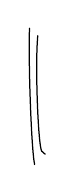
\begin{tikzpicture}[x=1cm,y=1cm,line width=.45pt,line cap=round]
\draw (0,0) .. controls (-.015,-.48) and (.025,-1.54) .. (.065,-1.73);
\draw (.105,-.095) .. controls (.070,-.48) and (.110,-1.48) .. (.155,-1.56) .. controls (.165,-1.58) and (.185,-1.59) .. (.200,-1.60);
\end{tikzpicture}}}
\margin{\unsure{rappelons qu'on suppose} $\pi$ \unsure{anabélien|nonabélien}
$(2g+\nu\geq3)$}
\[
1\longrightarrow\pi'\longrightarrow
\widehat{\widehat{\mathcal T}}(\pi,i)\longrightarrow
\unsure{\widehat{\widehat{\mathcal G}}}(\pi',i)\longrightarrow1
\]
ou encore
\[
1\longrightarrow\widehat{\pi}_{g,\nu-1}\longrightarrow
\widehat{\widehat{\mathcal T}}_{g,(\nu,\nu-1)}
\longrightarrow\unsure{\widehat{\widehat{\mathcal G}}}_{g,\nu-1}
\longrightarrow1
\]
qui contient la suite exacte
\[
1\longrightarrow\pi_{g,\nu-1}^{\unsure{*|+}}\longrightarrow
\mathcal T_{g,(\nu,\nu-1)}\longrightarrow
\unsure{\mathcal G}_{g,\nu-1}\longrightarrow1
\]
\unsure{comme|connue} sous\deleted{\unsure{particulière|partie dense}}, \unsure{suite|est} exacte.
Il est commode de travailler plutôt avec
\diagram{\begin{tikzcd}[ampersand replacement=\&,column sep=2.1em,row sep=3.0em]
1 \arrow[r,dash] \&
\pi_{g,\nu-1} \arrow[r,dash] \arrow[d,hook',no head] \&
\unsure{\mathcal T}_{g,\nu}^{!+} \arrow[r] \arrow[d,hook',no head] \&
\mathcal G_{g,\nu-1}^{!+} \arrow[r,dash] \arrow[d,hook',no head] \& 1 \\
1 \arrow[r,dash] \&
\widehat{\pi}_{g,\nu-1} \arrow[r] \arrow[d,equal] \&
\underset{\deleted{\unsure{\illegible{1}}}}{\widehat{\mathcal T}_{g,\nu}^{!+}}
\arrow[r] \arrow[d,hook',no head] \&
\widehat{\mathcal G}_{g,\nu-1}^{!+} \arrow[r,dash] \arrow[d,hook'] \& 1 \\
1 \arrow[r,dash] \&
\widehat{\pi}_{g,\nu-1} \arrow[r] \&
\widehat{\widehat{\mathcal T}}_{g,\nu}^{!} \arrow[r] \&
\widehat{\widehat{\mathcal G}}_{g,\nu-1}^{!} \arrow[r,dash] \& 1
\end{tikzcd}}

L'application $\unsure{\text{Prédiscrét}|\text{Prédiscrit}}^{+}(\pi)\longrightarrow
\unsure{\text{Prédiscrét}|\text{Prédiscrit}}^{+}(\pi')$ s'identifie donc à
$\widehat{\widehat{\mathcal T}}_{g,\nu}^{!}/\widehat{\mathcal T}_{g,\nu}^{!}$,
on lit sur le diagramme que c'est
$\simeq\widehat{\widehat{\mathcal G}}_{g,\nu-1}^{\unsure{!}\deleted{\unsure{+}}}/
\widehat{\mathcal G}_{g,\nu-1}^{!+}$,
d'où la bijectivité sur les ens des prédiscrétifications orientées.

Dans le groupe $\widehat{\widehat{\mathcal T}}_{g,\nu}^{!}=\mathcal T$,
on a un sous-groupe invariant $\widehat{\pi}_{g,\nu-1}=\pi'$,
et un sous-groupe $\Sigma$ $(\unsure{=|\longleftarrow}\widehat{\mathcal T}_{g,\nu}^{!+})$
\mspage{347}

\scanpage{349}

entre $\pi'$ et $\mathcal T$, \deleted{\unsure{donnant par}} \inserted{donnant} un ss-groupe $\Sigma'\simeq\mathcal T(\pi')$\inserted{$(=\unsure{\widehat{\mathcal G}^{!+}_{g,\nu-1}})$} dans $\unsure{\mathcal T'}=\mathcal T/\pi'$ $(\simeq\widehat{\widehat{\mathcal G}}^{!}_{g,\nu-1})$, et on sait bien qu'alors
\[
\mathcal T/\Sigma\simeq\mathcal T'/\Sigma',
\]
et \deleted{$\unsure{N(\Sigma)}$} que le normalisateur \inserted{$\mathcal N$,} de $\Sigma$ dans $\mathcal T$ est l'image inverse du normalisateur $\mathcal N'$ de $\Sigma'$ dans $\mathcal T'$, de sorte que $\mathcal N/\Sigma\simeq\mathcal N'/\Sigma'$, ce qui prouve ce qu'on voulait.

\uline{Corollaire} On a des \unsure{is.} canoniques
\[
\Gamma_{g,\nu}\xrightarrow{\sim}\Gamma_{g,\nu-1}\xrightarrow{\sim}\unsure{\cdots}\quad\deleted{\unsure{\Gamma_{g,0}}}
\]
\margin{On voit aussi que $\unsure{\Sigma|\Sigma^{!}}$ invariant dans $\unsure{\mathcal T|\widehat{\widehat{\mathcal T}}}$ équivaut à $\Sigma'$ invariant dans $\widehat{\widehat{\mathcal T}}'$}
de sorte que si $g\geq2$, on a \unsure{canoniqt} $\Gamma_{g,\nu}\simeq\Gamma_{g,0}$, d'autre part $\Gamma_{1,\nu}\simeq\Gamma_{1,1}$ $(g=1,\nu\geq1)$, $\Gamma_{0,\nu}\simeq\Gamma_{0,3}$ $(\nu\geq3)$.

\uline{NB} Le ``fait'' \deleted{\illegible{1}} admis est loin d'être évident --- même que $\widehat{\widehat{\mathcal T}}^{\unsure{!}}_{g,(\nu,\nu-1)}\longrightarrow\unsure{\widehat{\widehat{\mathcal T}}_{g,\nu-1}|\widehat{\widehat{\mathcal M}}_{g,\nu-1}}$ soit surjectif, ou que $\widehat{\widehat{\mathcal T}}_{g,(\nu,\nu-1)}\longrightarrow\widehat{\widehat{\mathcal G}}_{g,\nu-1}$ soit injectif, est loin d'être évident, et est peut-être tout à fait faux !

Le fait admis revient à un énoncé d'existence d'un foncteur \unsure{en} sens inverse ``forage des trous'', \unsure{qui|quid} en tout état de cause reste incompris.

\mspage{348}

\scanpage{350}
\mspage{177}

28. \uline{Changement de type} $(g,\nu)$ \unsure{(suite)} : \uline{\unsure{passage} à un rev. fini.}

Soit $\pi$ un groupe profini \inserted{à lacets} de type $(g,\nu)$, anabélien comme tjrs, $\pi'$ un ss-groupe d'indice fini. On sait (\unsure{ou on|on en} vérifie, par passage au cas discret) que \deleted{\illegible{1} \unsure{discrétifié}} \inserted{muni des} \unsure{traces} \unsure{sur|sous} $\pi$ des ss-groupes à \unsure{lacets} de $\pi$, $\pi'$ est un groupe à lacets.

\deleted{Si pour tout $i\in I(\pi)$, on considère un $L_i$, et les $\unsure{n}$ conjugués $\unsure{\operatorname{int}(g)}L_i$ \inserted{$=L_{i\alpha}$}, avec $g\in\pi\bmod\pi'$ $(n=[\pi:\pi']\unsure{\}},\ \deleted{\unsure{n}}\ \inserted{1\leq\alpha\leq n})$ \deleted{\unsure{comptés|compter} le nb de fois qu'une classe de conjugaison dans $\pi'$ du ss-groupe $\unsure{\operatorname{int}(g)}L_i$ est} \inserted{alors si $\unsure{d_{\alpha}|d_{i\alpha}}=[L_{i\alpha}:\unsure{L'_{i\alpha}|N'_{i\alpha}}\deleted{\unsure{\cap\pi'}}]$ \unsure{pour} $L'_{i\alpha}=L_{i\alpha}\cap\pi'$, alors} exactement $d_{i\alpha}$ parmi les $L'_{i\beta}$ \inserted{$(1\leq\beta\leq n)$} sont conjugués dans $\pi'$ à $L'_{i\alpha}$, et si on somme sur les classes de \unsure{conjugaison} distinctes des sous-groupes}

Les sous-groupes à lacets sont \unsure{aussi|ainsi} les \deleted{\unsure{les}} sous-groupes $L'$ tels que
\[
\text{a)}\quad L'=\operatorname{Centr}_{\pi}(L')\cap\pi'.
\]
\[
\text{b)}\quad L\unsure{=|:}\operatorname{Centr}_{\pi}(L')\text{ est un sous-groupe à \unsure{lacet} dans }\pi.
\]
On pose $d(L')=[L:L']$, et on a ainsi une fonction
\[
d:I'=I(\pi')\longrightarrow\mathbb N^*,
\]
et une application $I'\xrightarrow{\varphi}I$, telles que $\forall i\in I$, on ait
\[
\text{(1)}\qquad \sum_{\substack{i'\in I'\\\text{sur }i}}d(i')=n
\qquad (\text{\unsure{où|ici}}\ n=[\pi:\pi'])
\]
On aura la formule de Hurwitz
\[
\text{(2)}\qquad \deleted{\unsure{2g|2\alpha}}\ 2g'-2=n(2g-2)+\overbrace{\sum_{i'\in I'}(d(i')-1)}^{\inserted{n\operatorname{card}I-\operatorname{card}I'}}
\]
\mspage{349}
\scanpage{351}
i.e.
\[
(3)\qquad 2g'-2+\mathrm{card}\,I'=n(2g-2+\mathrm{card}\,I)
\]

(NB. \deleted{\unsure{\(n\)}} \((2g-2+\mathrm{card}\,I)\) est
\inserted{l'opposé de} la \unsure{car.} d'EP à supports
compacts de la courbe dont \(\unsure{\Pi|\pi}\) est le groupe
fondamental\ldots) \(\checkmark\)

\margin{\uline{NB} dire qu'on \unsure{est} dans le cas
\unsure{anabélien} signifie que \(-\mathrm{EP}_{!}\) est \(\geq 1\)
--- cette \unsure{condition|relation} est \unsure{donc conservée}
par passage \unsure{à un revêtement|aux revêtements}.
L'entier \(-\mathrm{EP}_{!}\) \unsure{mesure} \unsure{positivité stricte}
\illegible{1} degré d'\unsure{anabélianité}, \unsure{en qq sorte}\ldots}

De façon évidente, \unsure{tte} discrétification de \(\unsure{\Pi|\pi}\)
en définit une de \(\unsure{\Pi|\pi}'\) --- et il en est de
\(\overline{\mathrm m}\) pour les discrétifications orientées, modulo
un peu de cohomologie [qui revient à dire,
\inserted{dans le cas \unsure{discret} \unsure{pex|p.ex})}
que
\diagram{\begin{tikzcd}[ampersand replacement=\&]
H^2_{!}(\unsure{U|\mathcal U},\unsure{\mathbb Z|\mathbf Z}) \arrow[r] \arrow[d,phantom,sloped,"\simeq"] \& H^2_{!}(\unsure{U'|\mathcal U'},\unsure{\mathbb Z|\mathbf Z}) \arrow[d,phantom,sloped,"\simeq"] \\
T \& T'
\end{tikzcd}}
peut s'écrire sous la forme \(n\theta^{-1}\), où \(\theta\) est un iso. bien
déterminé (l'isom. trace) \unsure{\(\theta\)|de} \(T'\xrightarrow{\sim}T\).

Il n'est pas clair pour moi à première
vue si l'application
\[
\mathrm{Discret}(\unsure{\Pi|\pi})\unsure{-|\longrightarrow}\mathrm{Discret}(\unsure{\Pi|\pi}')
\]
est surjective, ou injective. L'injectivité
\inserted{(pour \unsure{tt} \(\unsure{\Pi|\pi}'\) d'indice fini de \(\unsure{\Pi|\pi}\))}
signifierait que : deux discrétifications \(\unsure{\Pi|\pi}_0,\unsure{\Pi|\pi}'_0\) de
\(\unsure{\Pi|\pi}\) qui sont commensurables, i.e. telles que
\(\unsure{\Pi|\pi}_0\cap\unsure{\Pi|\pi}'_0\) soit d'indice fini dans \(\unsure{\Pi|\pi}_0\) et dans \(\unsure{\Pi|\pi}'_0\),
\deleted{en fait, il suffit \unsure{qu'il le soit} dans l'un d'eux}
\inserted{égales}

\scanpage{352}
\mspage{178}
Supposons que \(\unsure{\Pi|\pi}'\) soit sous-groupe invariant
dans \(\unsure{\Pi|\pi}\), posons \(G=\unsure{\Pi|\pi}'/\unsure{\Pi|\pi}\)

\uline{Conjecture} L'application \(\mathrm{Discret}(\unsure{\Pi|\pi})\longrightarrow\mathrm{Discret}(\unsure{\Pi|\pi}')\)
est injective, et son image est formée des
discrétifications \(\unsure{\Pi|\pi}'_0\subset\unsure{\Pi|\pi}'\) telles que
\(G\longrightarrow\mathrm{Aut\,ext}_{\mathrm{lac}}(\unsure{\Pi|\pi}')
\simeq\mathrm{Aut\,ext}_{\mathrm{lac}}(\widehat{\unsure{\Pi|\pi}}'_0)
\simeq\widehat{\widehat{\mathcal T}}(\widehat{\unsure{\Pi|\pi}}'_0)\)
se factorise par \(\mathcal T(\unsure{\Pi|\pi}'_0)=\mathrm{Autext}_{\mathrm{lac}}(\unsure{\Pi|\pi}'_0)\)
(et en fait, \(\overline{\mathrm m}\) par \(\mathcal T(\unsure{\Pi|\pi}'_0)^+\)).

\margin{En d'autres termes, \(\forall g\in\unsure{\Pi|\pi}\),
\(\exists h\in\unsure{\Pi|\pi}'\) tel que \(\mathrm{int}(hg)(\unsure{\Pi|\pi}'_0)\subset\unsure{\Pi|\pi}'_0\)
i.e. \(\unsure{\unsure{\Pi|\pi}'|\unsure{\Pi|\pi}'_0}\cdot\unsure{\Pi|\pi}_0=\unsure{\Pi|\pi}\), où \(\unsure{\Pi|\pi}_0\) est le
normalisateur de \(\unsure{\Pi|\pi}'_0\) dans \(\unsure{\Pi|\pi}\).}

La condition pour qu'un \deleted{\illegible{1}} \(\unsure{\Pi|\pi}'_0\) soit dans
l'image est évidemment nécessaire. Montrons
qu'elle est suffisante, et que le \(\unsure{\Pi|\pi}_0^{\unsure{*}}\) donnant
\unsure{naissance} à \(\unsure{\Pi|\pi}'_0\) par \(\unsure{\Pi|\pi}_0\cap\unsure{\Pi|\pi}'\) est unique.
On a une action extérieure de \(G\) sur \(\unsure{\Pi|\pi}'_0\),
qui définit l'action extérieure sur \(\widehat{\unsure{\Pi|\pi}}'_0\simeq\unsure{\Pi|\pi}'\),
or \(\unsure{\Pi|\pi}\) se récupère canoniquement à partir de
cette dernière (car \(\mathrm{Centre}(\widehat{\unsure{\Pi|\pi}}')=1\)), et on
voit que c'est l' \deleted{adhérence dans} \inserted{complété} profini de
l'extension \inserted{\(\unsure{\Pi|\pi}_0\)} de \(G\) par \(\unsure{\Pi|\pi}'_0\), définie par l'action
\inserted{ext.} de \(G\) sur \(\unsure{\Pi|\pi}'_0\). On a donc bien une
discrétification généralisée \inserted{\(\unsure{\Pi|\pi}_0\) de \(\unsure{\Pi|\pi}\)}, au sens de la
seule structure de \deleted{\unsure{gr}} groupe profini, et elle
induit \(\unsure{\Pi|\pi}'_0\) --- mais il faut voir qu'elle
est compatible avec la structure à lacets de \(\unsure{\Pi|\pi}\).

\scanpage{353}
Mais celle-ci s'explicite, à partir de la
structure à lacets de \(\unsure{\Pi|\pi}'\), on prend les
sous-groupes à lacets \inserted{\(L'\)} de \(\unsure{\Pi|\pi}'\), et leurs
Centralisateurs dans \(\unsure{\Pi|\pi}\). Faisons \unsure{itou} pour
\(\unsure{\Pi|\pi}_0\unsure{\supset|>}\unsure{\Pi|\pi}'_0\), on devrait trouver une structure
à lacets sur \(\unsure{\Pi|\pi}_0\), donnant lieu aux
\(\overline{\mathrm m}\)\unsure{s} \(d_i\).
J'ai l'impression que ça ne
doit pas être très vache à prouver --- ce
serait comme si on savait déjà que \unsure{tte}
extension \inserted{``sans torsion''} d'un groupe fini par un
groupe à lacets est (de la façon canonique)
un groupe à lacets\ldots

\uline{Corollaire} En tous cas, l'application
\(\mathrm{Discret}(\unsure{\Pi|\pi})\longrightarrow\mathrm{Discret}(\unsure{\Pi|\pi}')\)
est \uline{injective}.
\figure{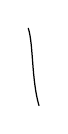
\begin{tikzpicture}[x=1cm,y=1cm,line width=.45pt,line cap=round]
\draw (0,0) .. controls (.065,-.20) and (.040,-.65) .. (.135,-.98);
\end{tikzpicture}}

\uline{NB} Elle ne doit pas tjs être bijective,
car il doit y avoir une action \inserted{\unsure{extérieure|extérieures}} d'un
\(G\) dans un \(\widehat{\unsure{\Pi|\pi}}'_0\) i.e. des hom
\(G\longrightarrow\widehat{\widehat{\mathcal T}}(\widehat{\unsure{\Pi|\pi}}'_0)\), qui ne se \unsure{factorise|factorisent} pas
par \(\mathcal T(\unsure{\Pi|\pi}'_0)\), et qui pourtant est aussi
\unsure{bonne|bonnes} du pt de vue groupe profini que
\unsure{celle|celles} provenant d'un \(\unsure{\Pi|\pi}\) et d'un \unsure{ss-groupe}

\scanpage{354}
\mspage{179}

invariant $\unsure{\Pi|\pi}'$. En fait, partons d'une telle situation \uline{discrète} $\unsure{\Pi|\pi}_0 \unsure{\supset|>} \unsure{\Pi|\pi}'_0$, d'où $G=\unsure{\Pi|\pi}_0/\unsure{\Pi|\pi}'_0$ et $G\longrightarrow \operatorname{Autext}_{\mathrm{lac}}(\unsure{\Pi|\pi}'_0)\deleted{\unsure{(\pi'_0)}}=\mathcal T(\unsure{\Pi|\pi}'_0)\subset\unsure{\widehat{\mathcal T}|\widehat{\widehat{\mathcal T}}}(\widehat{\unsure{\Pi|\pi}}'_0)$, et \uline{conjuguons} $G$ par un élément \inserted{$\gamma$} de $\widehat{\widehat{\mathcal T}}(\unsure{\Pi|\pi}'_0)$, de façon à trouver $G\longrightarrow\widehat{\mathcal T}(\widehat{\unsure{\Pi|\pi}}'_0)$ qui ne \deleted{\illegible{2}} se \unsure{factorise} pas par $\mathcal T(\unsure{\Pi|\pi}^{\unsure{'}}_0)$. On trouve une extension \inserted{$\unsure{\widehat{\unsure{\Pi|\pi}}|\unsure{\Pi|\pi}}^{\unsure{\natural|\sharp}}$} de $G$ par $\widehat{\unsure{\Pi|\pi}}'_0$, \uline{isomorphe} à $\widehat{\unsure{\Pi|\pi}}_0$ (en tant qu'extension de $G$ par $\widehat{\unsure{\Pi|\pi}}'_0$), donc la structure à lacets de $\widehat{\unsure{\Pi|\pi}}'_0$ en définit une sur $\unsure{\Pi|\pi}^{\unsure{\natural|\sharp}}$ \deleted{et est} \inserted{(de façon à être} induite par cette dernière), mais pourtant la discrétification \uline{choisie} \inserted{$\unsure{\Pi|\pi}_0$} de $\widehat{\unsure{\Pi|\pi}}_0$ n'est pas induite par une de $\unsure{\Pi|\pi}$. Pour

$\ast$ Faire la construction, il suffit de trouver un élément \inserted{$\gamma\in\widehat{\widehat{\mathcal T}}(\unsure{\Pi|\pi}'_0)$ \deleted{\unsure{fini}} tel que $\operatorname{int}(\gamma).G\unsure{\not\subset|\notin}\mathcal T$,} \deleted{\unsure{$u$} \unsure{d'ordre} \illegible{1} \unsure{provenant} pas de, \unsure{dans} $\mathcal T(\unsure{\Pi|\pi}'_0)$, \unsure{ou se} \unsure{relevant} par un élément d'ordre fini de $\unsure{\mathcal G|\mathcal C}(\unsure{\Pi|\pi}'_0)^+=\operatorname{Aut}_{\mathrm{lac}}(\unsure{\Pi|\pi}'_0)^+$, et \deleted{dont la \unsure{conjugaison} dans $\widehat{\widehat{\mathcal T}}$ \unsure{un}} \inserted{un $\gamma\in\widehat{\widehat{\mathcal T}}(\unsure{\Pi|\pi}'_0)$, tel que} $\gamma u\gamma^{-1}\notin\mathcal T(\unsure{\Pi|\pi}'_0)$, \inserted{\deleted{i.e. tel que $u$ ne \unsure{fixe}}} \deleted{pas} \inserted{$\gamma^{-1}.\unsure{\Pi|\pi}'_0\subset\widehat{\unsure{\Pi|\pi}}'_0$.}}
\figure{[Une grande partie du passage annulé est entourée d'un cadre (côtés gauche, inférieur et droit) et barrée de quatre longs traits obliques. Après l'inclusion $\gamma^{-1}.\unsure{\Pi|\pi}'_0\subset\widehat{\unsure{\Pi|\pi}}'_0$ de la dernière ligne, trait recourbé en crochet, dirigé vers l'inclusion suivante.]}
\inserted{i.e. tel que $G$ \deleted{\unsure{ne fixe}} ne stabilise pas $\gamma^{-1}(\unsure{\Pi|\pi}'_0)\subset\widehat{\unsure{\Pi|\pi}}'_0$}

Un tel $\gamma$ existe \unsure{tjrs}....

\scanpage{355}

Bien sûr, il n'y a pas de raison, \deleted{que} pour deux discrétifications $\unsure{\unsure{\Pi|\pi}'_0|\unsure{\Pi|\pi}_0},\unsure{\Pi|\pi}_1$ de $\unsure{\Pi|\pi}$, que si $\unsure{\Pi|\pi}_0,\unsure{\Pi|\pi}_1$ sont $\unsure{\Pi|\pi}$-conjugués (i.e. définissent \deleted{des} \inserted{la $\overline{\mathrm m}$} \unsure{prédiscrt.|prédiscrét.} stricte\deleted{s} de $\unsure{\Pi|\pi}$), il en soit de $\overline{\mathrm m}$ pour $\unsure{\Pi|\pi}'_0$ et $\unsure{\Pi|\pi}'_1$ pour l'action intérieure de $\unsure{\Pi|\pi}'$. (Il faudrait que $\unsure{\Pi|\pi}_0,\unsure{\Pi|\pi}_1$ soient conjugués par $\unsure{\Pi|\pi}'$, et pas seulement par $\unsure{\Pi|\pi}$). Par contre, je présume que si $\unsure{\Pi|\pi}_0,\unsure{\Pi|\pi}_1$ sont ``adhérents'' l'un à l'autre dans l'espace des \unsure{discrétifications|discrétific.} de $\unsure{\Pi|\pi}$, i.e. s'ils définissent une $\overline{\mathrm m}$ prédiscrétification, il en va de $\overline{\mathrm m}$ pour $\unsure{\Pi|\pi}'_0,\unsure{\Pi|\pi}'_1$, et que l'application
\[
\tag{4}
\operatorname{Prédiscrt}^{+}(\unsure{\Pi|\pi}\deleted{\unsure{_0}})\longrightarrow\operatorname{Prédiscrt}^{+}(\unsure{\Pi|\pi}'\deleted{\unsure{_0}})
\]
qu'on obtient ainsi, est encore bijective, et qu'elle passe à son tour au quotient, pour définir une application bijective
\[
\tag{5}
\unsure{\operatorname{Préarith}|\operatorname{Préarithm}}(\unsure{\Pi|\pi}\deleted{\unsure{_0}})\longrightarrow\unsure{\operatorname{Préarith}|\operatorname{Préarithm}}(\unsure{\Pi|\pi}'\deleted{\unsure{_0}}),
\]
et que si $\Sigma,\Sigma'$ se correspondent par cette dernière, qu'on a un isom canonique
\[
\tag{6}
\unsure{\mathbb{\Gamma}|\Gamma}_{\Sigma}\longrightarrow\unsure{\mathbb{\Gamma}|\Gamma}_{\Sigma'},
\]
\unsure{comp.$^{\mathrm t}$ble},

\scanpage{356}
\mspage{180}

avec les actions de ces groupes sur l'ens $P_{\Sigma}$ des prédiscrétifications de $\unsure{\Pi|\pi}$ comp.tibles à $\Sigma$, et l'ens \inserted{$P_{\Sigma'}$} des prédiscrétifications de $\unsure{\Pi|\pi}'$ comp.tibles à $\Sigma'$ (qui sont resp. des torseurs à g. sous $\unsure{\mathbb{\Gamma}|\Gamma}_{\Sigma},\unsure{\mathbb{\Gamma}|\Gamma}_{\Sigma'}$). En même temps, on trouvera \inserted{donc} que $\Sigma$ est unique pour $\unsure{\Pi|\pi}$ i.e. invariant dans $\widehat{\widehat{\mathcal T}}(\unsure{\Pi|\pi})$, ssi $\Sigma'$ est unique dans $\unsure{\Pi|\pi}'$ i.e. invariant dans $\widehat{\widehat{\mathcal T}}(\unsure{\Pi|\pi}')$.

En tous cas, la conjecture fondamentale qui \unsure{interprète} les $\unsure{\mathbb{\Gamma}|\Gamma}_{g,\unsure{\nu|v}}$ comme $\unsure{\mathbb{\Gamma}|\Gamma}_0=\operatorname{Gal}(\overline{\mathbb Q}_0/\mathbb Q)$ \unsure{aurait|aura} au moins comme conséquence que l'application $\operatorname{Discr}^{+}(\unsure{\Pi|\pi})\unsure{-|\longrightarrow}\operatorname{Discr}^{+}(\unsure{\Pi|\pi}')$ passe au quotient \inserted{de} deux façons, pour donner un diagramme comm.

\diagram{
\begin{tikzcd}[row sep=large,column sep=large,ampersand replacement=\&]
\operatorname{Discr}^{+}(\unsure{\Pi|\pi}) \arrow[r,no head] \arrow[d]
  \& \operatorname{Discr}^{+}(\unsure{\Pi|\pi}') \arrow[d] \\
\unsure{P|p}=\unsure{\operatorname{Prédiscr}}^{+}(\unsure{\Pi|\pi}) \arrow[r] \arrow[d]
  \& \unsure{P|p}'=\operatorname{Prédiscr}^{+}(\unsure{\Pi|\pi}') \arrow[d] \\
A=\operatorname{Arithm}(\unsure{\Pi|\pi}) \arrow[r]
  \& A'=\operatorname{Arithm}(\unsure{\Pi|\pi}')
\end{tikzcd}
}

et que le \deleted{\unsure{diagr|diagr.}} carré inférieur est cartésien (sans préjuger de l'\unsure{injectivité} ou de la \unsure{bijectivité} de l'application $A\longrightarrow A'$). \unsure{Donc} il faudrait

\scanpage{357}
que \deleted{\unsure{déjà}} si $\unsure{\Pi|\pi}_0,\unsure{\Pi|\pi}_1$ sont deux discrétifications \inserted{(\unsure{orientées})} de $\unsure{\Pi|\pi}$, qui définissent la $\overline{\mathrm m}$ prédiscrétification (\unsure{orientée}), alors il en va de $\overline{\mathrm m}$ pour \inserted{leurs \unsure{traces} sur $\unsure{\Pi|\pi}'$,} $\unsure{\Pi|\pi}'_0$ \unsure{et} $\unsure{\Pi|\pi}'_1$, relativement à $\unsure{\Pi|\pi}'$. Mais déjà si $\unsure{\Pi|\pi}_0$ et $\unsure{\Pi|\pi}_1$ sont $\unsure{\Pi|\pi}$-conjugués (i.e. définissent $\overline{\mathrm m}$ discrét. (\unsure{orientée}, \uline{\unsure{stricte}})), ce n'est pas tellement clair --- \deleted{\unsure{à moins de}} mais si, car on aura $\unsure{\Pi|\pi}=\unsure{\Pi|\pi}'\cdot\unsure{\Pi|\pi}_0$ donc si $\unsure{\Pi|\pi}_1=\operatorname{int}(u)\unsure{\Pi|\pi}_0$ écrivant $u=u'u_0$ avec $u'\in\unsure{\Pi|\pi}'$, $u_0\in\unsure{\Pi|\pi}_0$, on aura
\[
\unsure{\Pi|\pi}_1=\operatorname{int}(u')\operatorname{int}(u_0)\unsure{\Pi|\pi}_0=\operatorname{int}(u')\unsure{\Pi|\pi}_0,
\]
donc $\unsure{\Pi|\pi}'_1=\operatorname{int}(u')\unsure{\Pi|\pi}'_0$ donc $\unsure{\Pi|\pi}'_0$ et $\unsure{\Pi|\pi}'_1$ sont conjugués.

Tâchons de procéder de $\overline{\mathrm m}$ dans le cas général d'un $u\in\widehat{\unsure{\mathcal{C}|\mathcal{G}}(\unsure{\Pi|\pi}_0)}^+$, \inserted{tel que $\unsure{\Pi|\pi}_1=u(\unsure{\Pi|\pi}_0)$,} en écrivant si possible $u=u'u_0$, avec $u'\in\widehat{\unsure{\mathcal{C}|\mathcal{G}}(\unsure{\Pi|\pi}_0,\unsure{\Pi|\pi}'_0)}^+$, et $u_0\in\unsure{\mathcal{C}|\mathcal{G}}(\unsure{\Pi|\pi}_0)^+$, où on définit $\unsure{\mathcal{C}|\mathcal{G}}(\unsure{\Pi|\pi}_0,\unsure{\Pi|\pi}'_0)^+$ comme le groupe des \unsure{i-automs|l-automs} \inserted{\unsure{directs|discrets}} de $\unsure{\Pi|\pi}_0$ qui \uline{stabilisent $\unsure{\Pi|\pi}'_0$}, et $\widehat{\unsure{\mathcal{C}|\mathcal{G}}}(\unsure{\Pi|\pi}_0,\unsure{\Pi|\pi}'_0)^+$ est son \unsure{compactifié} profini. On aurait alors $\unsure{\Pi|\pi}_1=u'(u_0(\unsure{\Pi|\pi}_0))=\dot{u}'(\unsure{\Pi|\pi}_0)$, où \deleted{\illegible{1}} $\dot{u}'$ désigne l'image de $u'$ dans $\widehat{\unsure{\mathcal{T}|\mathcal{C}}(\unsure{\Pi|\pi}'_0)}$. En tous cas, il n'y a aucun Pb si $\unsure{\Pi|\pi}'\deleted{\unsure{_0}}$ est un ss-groupe \deleted{\unsure{fermé}} \uline{caractéristique} de $\unsure{\Pi|\pi}$, car alors on a un hom

\scanpage{358}
\mspage{181}
discret $\unsure{\mathcal{C}|\mathcal{G}}(\unsure{\Pi|\pi}_0)\longrightarrow\unsure{\mathcal{C}|\mathcal{G}}(\unsure{\Pi|\pi}'_0)$, définissant \unsure{l'|le} $\unsure{\widehat{\unsure{\mathcal{C}|\mathcal{G}}}(\widehat{\unsure{\Pi|\pi}}_0)}\longrightarrow\unsure{\widehat{\unsure{\mathcal{C}|\mathcal{G}}}(\widehat{\unsure{\Pi|\pi}}'_0)}$. Comme les sous groupes \unsure{ouverts} caract. de $\unsure{\Pi|\pi}$ sont cofinaux, on est ramené (pour les questions de factorisabilité \inserted{de $D(\unsure{\Pi|\pi})\longrightarrow D(\unsure{\Pi|\pi}')$ en $P(\unsure{\Pi|\pi})\longrightarrow P(\unsure{\Pi|\pi}')$ et $A(\unsure{\Pi|\pi})\longrightarrow A(\unsure{\Pi|\pi}')$} et de bijectivité des applications $\unsure{P}(\unsure{\Pi|\pi})\longrightarrow P(\unsure{\Pi|\pi}')$ et $A(\unsure{\Pi|\pi})\longrightarrow A(\unsure{\Pi|\pi}')$) on est ramené au cas où $\unsure{\Pi|\pi}'$ est ss-groupe \uline{caractéristique}. On a \unsure{bien|vu} \inserted{alors} \deleted{la} factorisabilité de $D(\unsure{\Pi|\pi})\longrightarrow D(\unsure{\Pi|\pi}')$ en $P(\unsure{\Pi|\pi})\longrightarrow P(\unsure{\Pi|\pi}')$, \inserted{\unsure{nous voulons}} \unsure{montrer|montrons} que cette application est injective \unsure{...} \inserted{Cela} \deleted{\unsure{cela signifie}}
\inserted{\textcircled{a}} signifie que l'image inverse dans $\widehat{\widehat{\unsure{\mathcal{C}|\mathcal{G}}}}(\widehat{\unsure{\Pi|\pi}}_0)$ de $\widehat{\unsure{\mathcal{C}|\mathcal{G}}}(\widehat{\unsure{\Pi|\pi}}'_0)^+$ est $\widehat{\unsure{\mathcal{C}|\mathcal{G}}}(\widehat{\unsure{\Pi|\pi}}_0)^+$, la surjectivité \inserted{\textcircled{b}} signifie que tt élément de $\widehat{\widehat{\unsure{\mathcal{C}|\mathcal{G}}}}(\widehat{\unsure{\Pi|\pi}}'_0)$ est congru mod $\widehat{\unsure{\mathcal{C}|\mathcal{G}}(\unsure{\Pi|\pi}'_0)}^+$ à un élément de l'image de $\widehat{\widehat{\unsure{\mathcal{C}|\mathcal{G}}}}(\unsure{\Pi|\pi}_0)$. La factorisabilité en $A(\unsure{\Pi|\pi})\longrightarrow A(\unsure{\Pi|\pi}')$ signifie que par \inserted{\textcircled{c}} l'application précédente \deleted{\unsure{de}} $\widehat{\widehat{\unsure{\mathcal{C}|\mathcal{G}}}}(\unsure{\Pi|\pi}_0)\hookrightarrow\widehat{\widehat{\unsure{\mathcal{C}|\mathcal{G}}}}(\unsure{\Pi|\pi}'_0)$, (NB il est immédiat que \unsure{c'est} injectif) \deleted{\unsure{est}} \inserted{envoie}
\[
M(\unsure{\Pi|\pi}_0)=\operatorname{Norm}_{\unsure{\widehat{\widehat{\mathcal{C}}}|\widehat{\mathcal{C}}}(\unsure{\Pi|\pi}_0)}\bigl(\widehat{\unsure{\mathcal{C}|\mathcal{G}}}^{+}(\unsure{\Pi|\pi}_0)\bigr)
\]
dans $M(\unsure{\Pi|\pi}'_0)$, l'injectivité de $A(\unsure{\Pi|\pi})\longrightarrow A(\unsure{\Pi|\pi}')$ que

\scanpage{359}

\textcircled{d} l'on a même \unsure{que} $M(\unsure{\Pi|\pi})$ est
\unsure{exactement|ex.\textsuperscript{t}} l'image inverse de $M(\unsure{\Pi|\pi}')$,
la \unsure{surjectivité} de
$A(\unsure{\Pi|\pi})\unsure{\twoheadrightarrow|\longrightarrow}A(\unsure{\Pi|\pi}')$ que
\inserted{\textcircled{e}} tt élément de
$\widehat{\widehat{\unsure{\mathcal C|\mathcal G}}}(\unsure{\Pi|\pi}'_0)$
est congru mod $M(\unsure{\Pi|\pi}'_0)$ à un élément de
$\widehat{\widehat{\unsure{\mathcal C|\mathcal G}}}(\unsure{\Pi|\pi}_0)$
\margin{plus faible que (b)}
--- et ces conditions \unsure{réunies} impliquent que l'hom canonique
\diagram{\begin{tikzcd}[ampersand replacement=\&]
\mathbb{\Gamma}_{\deleted{\unsure{\pi}}\unsure{\Pi|\pi}_0}
  \arrow[r] \arrow[d, equal]
  \& \mathbb{\Gamma}_{\unsure{\Pi|\pi}'_0} \arrow[d, equal] \\
M(\unsure{\Pi|\pi}_0)/\widehat{\unsure{\mathcal C|\mathcal G}}(\unsure{\Pi|\pi}_0)
  \& M^{\unsure{\sharp|*}}(\unsure{\Pi|\pi}'_0)/\widehat{\unsure{\mathcal C|\mathcal G}}(\unsure{\Pi|\pi}'_0)
\end{tikzcd}}
est iso -- il suffit $\overline{\mathrm m}$ pour ceci d'avoir
\unsure{(c)|(e)} (pour pouvoir définir cette application) et (a)
(pour son injectivité), et (b) et le renforcement (d) de
\unsure{(c)|(e)} (pour sa \unsure{bijectivité|surjectivité}. Donc on voit que
\unsure{tout} est suspendu aux propriétés de l'hom d'inclusions de groupes
\diagram{\begin{tikzcd}[ampersand replacement=\&,column sep=2.2em,row sep=3.8em,
execute at end picture={
  \draw[line width=.35pt] ([xshift=-6pt,yshift=-1pt]\tikzcdmatrixname-1-3.south) -- ([xshift=-9pt,yshift=-1pt]\tikzcdmatrixname-1-3.south) -- ([xshift=-9pt,yshift=1pt]\tikzcdmatrixname-2-3.north) -- ([xshift=-6pt,yshift=1pt]\tikzcdmatrixname-2-3.north);
  \draw[line width=.35pt] ([xshift=17pt,yshift=-1pt]\tikzcdmatrixname-1-3.south) -- ([xshift=20pt,yshift=-1pt]\tikzcdmatrixname-1-3.south) -- ([xshift=20pt,yshift=1pt]\tikzcdmatrixname-2-3.north) -- ([xshift=17pt,yshift=1pt]\tikzcdmatrixname-2-3.north);
}]
{} \arrow[d,phantom,"{(7)}"{description}] \&
\widehat{\mathcal G}^{+}(\pi_0)
\arrow[r,phantom,"{\subset}"{description}]
\arrow[d,hook,no head] \&
M(\pi_0)
\arrow[r,phantom,"{\subset}"{description}]
\arrow[d,hook]
\arrow[d,phantom,"{?}"{description,xshift=8pt}] \&
\widehat{\widehat{\mathcal G}}(\pi_0) \arrow[d,hook,no head] \\
{} \&
\widehat{\mathcal G}^{+}(\pi'_0)
\arrow[r,phantom,"{\subset}"{description}] \&
M(\pi'_0)
\arrow[r,phantom,"{\subset}"{description}] \&
\widehat{\widehat{\mathcal G}}(\pi'_0)
\end{tikzcd}}
à charge de prouver a) b) (qui ne \unsure{concernent} que le carré composé)
et \unsure{c)|e)}.

\deleted{D'ailleurs d) \unsure{sera} conséquence
\inserted{\unsure{immédiate}} de a), et du fait
(qui assurera \unsure{c)|e)}) que tt élément de
$\widehat{\unsure{\mathcal C|\mathcal G}}^{+}(\unsure{\Pi|\pi}_0)$ est congru mod
$\unsure{\mathcal C|\mathcal G}$}

\scanpage{360}
\mspage{182}

Peut. être les propriétés a) b) c) sont elles
tout à fait fausses -- pourtant a) (qui correspond à l'injectivité de
$P(\unsure{\Pi|\pi})\longrightarrow P(\unsure{\Pi|\pi}')$) semble assez plausible.
La propriété b) (qui exprimerait la surjectivité de
$P(\unsure{\Pi|\pi})\longrightarrow P(\unsure{\Pi|\pi}')$) est beaucoup plus problématique,
voir douteuse. L'ennui, c'est que le groupe
$\widehat{\widehat{\unsure{\mathcal C|\mathcal G}}}(\unsure{\Pi|\pi}_0)$
peut être ``beaucoup plus petit'' que
$\widehat{\widehat{\unsure{\mathcal C|\mathcal G}}}(\unsure{\Pi|\pi}'_0)$,
on s'en rend compte en passant au quotient par le sous-groupe
$\widehat{\unsure{\Pi|\pi}}'_0=\unsure{\Pi|\pi}'$ (contenu dans le plus petit des groupes de (7),
et invariant dans le plus grand), on trouve sur la deuxième ligne
les groupes $\widehat{\mathcal T}^{+}(\unsure{\Pi|\pi}'_0)$,
\deleted{\illegible{1}} $\unsure{\mathcal N|N}(\unsure{\Pi|\pi}'_0)$ et
$\widehat{\widehat{\mathcal T}}(\unsure{\Pi|\pi}'_0)$, sur la première
des extensions des groupes \unsure{corresp.dants|correspondants}
pour $\unsure{\Pi|\pi}_0$ ($\widehat{\mathcal T}^{+}(\unsure{\Pi|\pi}_0)$,
$\unsure{\mathcal N|N}(\unsure{\Pi|\pi}_0)$ et
$\widehat{\widehat{\mathcal T}}(\unsure{\Pi|\pi}_0)$) par
\inserted{le groupe fini} $G=\unsure{\Pi|\pi}_0/\unsure{\Pi|\pi}'_0\simeq\unsure{\Pi|\pi}/\unsure{\Pi|\pi}'$,
\deleted{\unsure{soient|soit}
$\unsure{\widetilde{\widehat{\mathcal T}}^{+}|\widetilde{\mathcal T}^{+}}$
ou $\mathcal T$}
\unsure{notées|notés} par des $\sim$, de sorte que \unsure{.|--}
\diagram{\begin{tikzcd}[ampersand replacement=\&,column sep=1.9em,row sep=3.8em,
execute at end picture={
  \draw[line width=.35pt] ([xshift=-6pt,yshift=-1pt]\tikzcdmatrixname-1-4.south) -- ([xshift=-9pt,yshift=-1pt]\tikzcdmatrixname-1-4.south) -- ([xshift=-9pt,yshift=1pt]\tikzcdmatrixname-2-4.north) -- ([xshift=-6pt,yshift=1pt]\tikzcdmatrixname-2-4.north);
  \draw[line width=.35pt] ([xshift=17pt,yshift=-1pt]\tikzcdmatrixname-1-4.south) -- ([xshift=20pt,yshift=-1pt]\tikzcdmatrixname-1-4.south) -- ([xshift=20pt,yshift=1pt]\tikzcdmatrixname-2-4.north) -- ([xshift=17pt,yshift=1pt]\tikzcdmatrixname-2-4.north);
}]
{} \arrow[d,phantom,"{(8)}"{description}] \&
G \arrow[r,phantom,"{\subset}"{description}] \arrow[dr,hook] \&
\widetilde{\widehat{\unsure{\mathcal T}}}^{+\unsure{:}}(\pi_0)
\arrow[r,phantom,"{\subset}"{description}]
\arrow[d,hook,no head] \&
\widetilde{\mathcal N}(\pi_0)
\arrow[r,phantom,"{\subset}"{description}]
\arrow[d,hook]
\arrow[d,phantom,"{?}"{description,xshift=8pt}] \&
\widetilde{\widehat{\widehat{\mathcal T}}}(\pi_0) \arrow[d,hook] \\
{} \& {} \&
\widehat{\mathcal T}^{+}(\pi'_0)
\arrow[r,phantom,"{\subset}"{description}] \&
\mathcal N(\pi'_0)
\arrow[r,phantom,"{\subset}"{description}] \&
\widehat{\widehat{\mathcal T}}(\pi'_0)
\end{tikzcd}},
qui montre que les groupes de la première ligne
\scanpage{361}
\uline{normalisent} le sous-groupe $G\subset\widehat{\mathcal T}^{+}(\pi'_0)$
(\uline{NB} en fait on a $G\subset\mathcal T^{+}(\pi'_0)$ ; \deleted{\illegible{1}} et $\pi_0$
se reconstitue à partir de $\pi'_0$ et de
ce sous-groupe de $\pi'_0$) --- \deleted{\unsure{je crois}}\inserted{on doit}
pouvoir montrer sans trop de mal
que \deleted{\illegible{1}} dans (8), $\widetilde{\widehat{\mathcal T}}^{+}(\pi_0)$ et $\widetilde{\widehat{\widehat{\mathcal T}}}(\pi_0)$
sont justement les normalisateurs de $G$
dans $\widehat{\mathcal T}^{+}(\pi'_0)$ et dans $\widehat{\widehat{\mathcal T}}(\pi'_0)$ (ce
qui impliquerait bien a), d'ailleurs) ---
mais je ne vois aucune raison plausible
que (b) soit vrai --- ce qui signifierait,
essentiellement, qu'il n'y a pas plus de
``\unsure{transcendance} arithmétique'' définie par le
(``très gros'' !) $\widehat{\widehat{\mathcal T}}(\pi'_0)$ (mod $\widehat{\mathcal T}(\pi'_0)^{+}$), que
celle définie par le (``bien plus petit'') groupe
$\widetilde{\widehat{\widehat{\mathcal T}}}(\pi_0)=\operatorname{Norm}_{\widehat{\widehat{\mathcal T}}(\unsure{\pi_0|\pi'_0})}(G)$ \dots\ D'ailleurs ces
conditions a) b) ne sont pas impératives
pour que la conjecture fondamentale
\unsure{reliant} les $\unsure{\pi_{g,\nu}|\Pi_{g,\nu}}$ à $\Gamma_0$ soit \unsure{cohérente} ---
\mspage{360}

\scanpage{362}
\mspage{183}
par contre il faudrait absolument avoir
c) pour pouvoir au moins définir
$A(\pi)\unsure{\longrightarrow|{-}}A(\pi')$ et (si $\Sigma,\Sigma'$ se correspondent)
$\Gamma_{\Sigma}\unsure{\longrightarrow|{-}}\Gamma_{\Sigma'}$, dans le cas $\unsure{\pi'_a|\pi'_0}$ \deleted{\unsure{invariant}}\inserted{caractéristique} dans $\pi$
(et dans tous les cas si on admet de plus
a), qui semble \unsure{assez} plausible, et donne
les \uline{injectivités} qu'il faut. Mais on
se demande bien pourquoi un élément
de \deleted{\illegible{1}} $\widehat{\widehat{\mathcal T}}(\pi'_0)$ simplement parce qu'
il \deleted{\unsure{normalise}}\inserted{est dans} le \deleted{$G$ et qu'il \unsure{normalise}}\inserted{normalisateur $R$ de $G$}
\deleted{\unsure{le même}}\inserted{dans} $\widehat{\widehat{\mathcal T}}(\pi'_0)$, \inserted{donc aussi $R$,} et qu'il normalise
$R\cap\widehat{\mathcal T}^{+}(\pi'_0)$, devrait normaliser aussi
$\widehat{\mathcal T}^{+}(\pi'_0)$ lui-$\overline{\mathrm m}$ ! Il est vrai qu'on a
fait des hypothèses \unsure{draconiennes} au départ
(\unsure{partant} d'un ss-groupe \uline{car.} $\pi'_0$ de $\pi_0$) qui
doivent bien se \unsure{refléter} par des propriétés
particulières de $G\subset\mathcal T^{+}(\pi'_0)$. Peut-être
finalement l'astuce de se ramener à des
ss-groupes caractéristiques pour examiner
\mspage{361}

\scanpage{363}
la situation n'est \unsure{elle} pas si astucieuse.
Pour y voir plus clair, on pourrait déjà
\unsure{essayer} de comprendre le cas où (sans
supposer $\pi'$ caract.) on suppose $\pi'$ d'indice
2 dans $\pi$, donc invariant et $G\simeq\mathbb Z/2$, ou
bien on prend \deleted{\illegible{2}} le noyau de l'hom
canonique $\pi\longrightarrow(\pi_{\mathrm{ab}})_2$ ($\simeq(\mathbb Z/2\mathbb Z)^{2g\deleted{+}}$ si $\nu=0$,
$\simeq(\mathbb Z/2\mathbb Z)^{2g\unsure{+|-}\nu-1}$ si $\nu\geq1$), en prenant p.ex.
$\pi=\widehat\Pi_{0,3}$ --- \unsure{situation} de la courbe de
Fermat $x^2+y^2+z^2=0$ (revêtement octaédral
de $\mathbb P^1_{\overline{\mathbb Q}}\setminus\{0,1,\infty\}$ \dots)

Mais admettons provisoirement les \deleted{résultats}\inserted{hypothèses}
d'injectivité (relativement anodines), \uline{plus} la
condition c), pas anodine du tout ---
d'où, si $\Sigma$ et $\Sigma'$ se correspondent, un hom
injectif
\[
(9)\qquad \Gamma_{\Sigma}\hookrightarrow\Gamma_{\Sigma'},
\]
et voyons ce qu'on pourrait en tirer.
en admettant même, provisoirement (pour
voir) que (9) est un iso --- \deleted{\unsure{Ce qui|Ce que}}
c'est à dire toute la force de la conjecture
principale $\Gamma_0\simeq\Gamma_{g,\nu}$.
\mspage{362}

\scanpage{364}
\mspage{184}

\unsure{Soient|Soit} $\pi$ un groupe profini \inserted{à lacets} de type $(g,\nu)$, $\pi'$ de type $(g',\nu')$. Appelons ``correspondance'' entre $\pi$ et $\pi'$ un \deleted{groupe} couple formé d'un $\unsure{G|\pi''}$ profini \inserted{à lacets} \deleted{de type $(g'',\nu'')$}, et d'hom. \inserted{à lacets} $\unsure{G|\pi''}\xrightarrow{p}\pi$, $\unsure{G|\pi''}\xrightarrow{q}\pi'$ qui sont donc \unsure{chacun|chacune} \unsure{composé|composée} d'un morphisme ``bouchage de trous'', et d'une \deleted{inclusion} isom. sur un \unsure{ss-groupe|ss-gr.} d'indice fini.
\unsure{Soit|Soient} $\unsure{J_p|I''_p}$, $\unsure{J_q|I''_q}\in\unsure{J|I''}=I(\pi'')$ les \inserted{ss-}ensembles de $\unsure{J|I''}$ qui correspondent aux ``trous bouchés par $p$'' resp. par $q$, on suppose \inserted{s'il le faut} $\unsure{J_p|I''_p}\cap\unsure{J_q|I''_q}=\varnothing$ (sinon on pourrait factoriser par un $\unsure{\overline{\mathrm m}}$ quotient $\widetilde{\pi}''$ de $\pi''$). En d'autres termes si $\unsure{\overline{J}_p|\overline{I}''_p}$, $\unsure{\overline{J}_q|\overline{I}''_q}$ sont les complémentaires de $\unsure{J_p|I''_p}$, $\unsure{J_q|I''_q}$ dans $\unsure{J|I''}$ (de sorte qu'on a : $\unsure{\overline{J}_p|\overline{I}''_p}\to I=I(\pi)$, $\unsure{\overline{J}_q|\overline{I}''_q}\to I'=I(\pi')$) on a
\[
\unsure{\overline{J}_p|\overline{I}''_p}\cup\unsure{\overline{J}_q|\overline{I}''_q}=\unsure{J|I''}.
\]

\deleted{\unsure{Utilisant|Utilisons} les ``résultats'' des deux \unsure{paragraphes} \unsure{antérieurs}, on définit alors des applications}

On va supposer maintenant $\pi$ muni d'un $\Sigma$ \inserted{$\in A(\pi)$}, $\pi'$ muni d'un $\Sigma'\in A(\pi')$, on appellera ``correspondance arithmétique'' entre $\pi$ et $\pi'$ un quadruple $(\unsure{G|\pi''},p,q,\unsure{\Sigma_G|\Sigma''})$, où $(\unsure{G|\pi''},p,q)$ sont comme dessus, et $\unsure{\Sigma_G^{a}|\Sigma_G}\in A(G)$, tels que l'on ait $\unsure{\Sigma_G|\Sigma_a}=p^*(\Sigma)=q^*(\Sigma')$. \deleted{\unsure{On supp}} Si $P_{\Sigma}$,
\mspage{363}

\scanpage{365}

$P_{\Sigma'}$, $P_{\unsure{\Sigma_G|\Sigma_a}}$ sont resp. les torseurs sous $\Gamma_{\Sigma}$, $\Gamma_{\Sigma'}$, $\Gamma_{\Sigma''}$ qu'on sait, on a deux \unsure{diagrammes|diagramme} d'isom. de torseurs
\diagram{\begin{tikzcd}[ampersand replacement=\&,column sep=small,row sep=large]
\& P_{\unsure{\Sigma_G|\Sigma_a}} \& \\
P_{\Sigma} \arrow[ur,"p_P^*","\sim"'] \& \& P_{\Sigma'} \arrow[ul,"q_P^*"',"\sim"]
\end{tikzcd}}
\diagram{\begin{tikzcd}[ampersand replacement=\&,column sep=small,row sep=large]
\& \Gamma_{\unsure{\Sigma_G|\Sigma''_G}} \arrow[dr,leftrightarrow,"q_\Gamma^*","\sim"'] \& \\
\Gamma_{\Sigma} \arrow[ur,"\unsure{\widehat{p}_\Gamma|p_\Gamma^*}","\sim"'] \& \& \Gamma_{\Sigma''}
\end{tikzcd}},
d'où par composition un \unsure{isom|hom} de
\deleted{$\unsure{P_{\Sigma}\to}$}
\[
(P_{\Sigma},\Gamma_{\Sigma})\xrightarrow{\sim}(P_{\Sigma'},\Gamma_{\Sigma'})
\]

On appelle ``isom arithmétiquement extérieurs'' \inserted{de $(\pi,\Sigma)$ avec $(\pi',\Sigma')$,} tout isomorphisme de torseurs qu'on peut obtenir de cette façon. Deux correspondances sont dites \inserted{\unsure{équivalentes} \deleted{\unsure{du point de}} du point de vue} \deleted{\unsure{arithmétiques|arithmétique} \unsure{extérieures|extérieure}} arithmétiquement extérieur, si elles définissent le $\unsure{\overline{\mathrm m}|=}$ isom. arithm. extérieur. \unsure{La} composition est définie par composition des actions sur $(P_{\Sigma},\Gamma_{\Sigma})$ --- on voit que \unsure{ça} provient d'une correspondance. On \unsure{trouve} donc un groupoïde, dont on vérifie sans peine qu'il est connexe. \inserted{Je dis que} Les autom de $(\pi,\Sigma)$ ``sont'' les autom de $(P_{\Sigma},\Gamma_{\Sigma})$ définis par des éléments de $\Gamma_{\Sigma}$. \deleted{C'est \unsure{évident} ou \unsure{pas}} C'est \unsure{facile}\ldots

\margin{On l'appellera le \unsure{groupoïde} des ``courbes arithmétiques extérieures''.}
\mspage{364}

\scanpage{366}
\mspage{185}

Dans ce groupoïde, il y a un syst. transitif d'iso. entre les \deleted{\illegible{1}} $(\widehat{\pi}_0,\overline{\Sigma}_{\pi_0})$ (où $\pi_0$ est un groupe discret à lacets) plus gén. entre les $(\pi,\Sigma_\alpha)$, où $\alpha$ \inserted{$\in P(\pi)$} est une prédiscrétification de $\pi$ --- définissons donc un isom. \inserted{arithmétiquement} extérieur de $\Pi_{g,\nu}$
$\pi$ \ldots\ \unsure{Le|Leur} groupe de \unsure{ces|ses} autom. est noté $\Gamma_0$. Le \deleted{catégorie} groupoïde des courbes \inserted{virtuelles} arithmétiques extérieures s'identifie donc à la cat. des torseurs sous $\Gamma_0$,
Une prédiscrétification (on pourrait aussi l'appeler une rigidification arithmétiquement extérieure) n'est \unsure{donc} autre chose qu' un isom arithm. extérieur entre cet élément de référence, et $\pi$.
\mspage{365}

\scanpage{367}
\mspage{186}

\uline{29} Critique de l'approche précédente.

L'approche \unsure{des|du} \S\ précédents semble \unsure{franchement|finalement} très brutale. J'ai même des doutes si \unsure{la|l'} \deleted{hypothèse} conjecture \unsure{dans|sur} les propriétés du foncteur "bouchage de trous" est vraie telle quelle. Il est vrai que pour un groupe profini \deleted{\illegible{1}} \inserted{\unsure{à}} \unsure{lacets} $\pi$, si on fixe $i\in I(\pi)$, on a un hom canonique
\[
\tag{1}
\widehat{\widehat{\mathcal T}}(\pi,i)
=\underset{\substack{\text{stabilisateur}\\\text{de }i\text{ dans }\widehat{\widehat{\mathcal T}}(\pi)}}{\text{\uline{$\widehat{\widehat{\mathcal T}}(\pi)_i$}}}
\longrightarrow \widehat{\widehat{\mathcal G}}(\pi'),
\]
mais il est problématique si c'est un isomorphisme --- et même si c'est injectif, ou si c'est surjectif. Mais, \unsure{choisissant} une discrétification $\pi_0\subset\pi$, d'où itou $\pi'_0$ pour $\pi'$, l'hom précédent induit bel et bien un isom
\[
\tag{1}
\mathcal T(\pi_0)_i\simeq\mathcal G(\pi'_0)
\]
d'où
\[
\tag{3}
\widehat{\mathcal T}(\pi_0)\xrightarrow{\sim}\widehat{\mathcal G}(\pi'_0)
\]
et par suite, la suite exacte $\deleted{\unsure{\widehat{\pi}_0}}\widehat{\pi}'_0\longrightarrow\widehat{\mathcal G}(\pi'_0)\longrightarrow\widehat{\mathcal T}(\pi'_0)\longrightarrow 1$ donne
\[
\tag{4}
1\longrightarrow\widehat{\pi}'_0\longrightarrow\widehat{\mathcal T}(\pi_0)\longrightarrow\widehat{\mathcal T}(\pi'_0)\longrightarrow 1
\]
et par suite on trouve un homomorphisme injectif
\[
\begin{gathered}\widehat{\pi}'_0\\[-0.5ex]\Vert\\[-0.5ex]\pi'\end{gathered}
\unsure{\hookrightarrow|\leftrightarrow}
\widehat{\mathcal T}(\pi_0)_i
\hookrightarrow
\begin{gathered}\widehat{\widehat{\mathcal T}}(\pi_0)_i\\[-0.5ex]\Vert\\[-0.5ex]\unsure{\widehat{\widehat{\mathcal T}}}(\pi)\end{gathered}
\]
donc un hom
\[
\tag{5}
i_{\pi_0}:\quad\pi'\longrightarrow\widehat{\widehat{\mathcal T}}(\pi)_i
\]
dont \unsure{le|la} composé avec (1) est l'injection canonique $\pi'\hookrightarrow\widehat{\widehat{\mathcal G}}(\pi')$. Remplaçant la discrétification \inserted{$\pi_0$} par une autre, $\pi_1$, on trouve a priori un autre hom $i_{\pi_1}:\pi'\longrightarrow\widehat{\widehat{\mathcal T}}(\pi)_i$. \unsure{OPS} $\pi_1=u(\pi_0)$, $u\in\widehat{\widehat{\mathcal T}}(\pi)_i$;

\mspage{366}

\scanpage{368}

et par transport de structure on trouve
\[
i_{\pi_1}=i_{u(\pi_0)}=\operatorname{int}(u)\circ i_{\pi_0}\circ u_{\pi'}^{-1}
\]
où $u_{\pi'}$ est l'automorphisme de $\pi'$ défini par $u$ via (1). Dire que $i_{\pi_0}$ est indépendant du choix de la discrétification $\pi_0$, revient aussi à dire que son image dans $\widehat{\widehat{\mathcal T}}(\pi)_i$ est un sous-groupe invariant --- et alors l'action de $\widehat{\widehat{\mathcal T}}(\pi)_i$ sur \deleted{\unsure{$\pi$}} le sous-groupe invariant $i_{\pi_0}(\pi)=i(\pi)$ \deleted{\illegible{1}} \unsure{via} \unsure{autom} intérieurs, n'est autre que celle définie par (1). \uline{Dans} ce cas, on trouve par passage au quotient un \unsure{homomorphisme}
\[
\tag{6}
\widehat{\widehat{\mathcal T}}(\pi)_i/\pi'\longrightarrow\widehat{\widehat{\mathcal T}}(\pi')
\]
dont l'injectivité resp. surjectivité équivaudrait à celle de (1). Mais il n'est pas évident du tout qu'il en soit \unsure{tjrs} ainsi.

S'il n'en était pas ainsi, il \deleted{serait} s'imposerait de regarder le sous-groupe de $\widehat{\widehat{\mathcal T}}(\pi)_i$ \inserted{formé des $\gamma\in\unsure{\widehat{\widehat{\mathcal T}}}(\pi)_i$ qui} \deleted{qui} normalisent le sous-groupe \deleted{\unsure{injecteur|injecté}} $i_{\pi_0}(\pi')$, et tels que l'action induite sur $i_{\pi_0}(\pi')$ correspond à celle donnée par l'action (1) de $\widehat{\widehat{\mathcal T}}(\pi)$ sur $\pi'$. Ce sous-groupe \inserted{$H_{\pi_0,\unsure{i}}$ (qui contient $\widehat{\mathcal T}(\pi_0)_i$) \deleted{\illegible{1}}} dépend donc a priori de la discrétification choisie. Remplaçant $\pi_0$ par $u(\pi_0)$ (où \deleted{\unsure{$u$}} $u\in\widehat{\widehat{\mathcal T}}(\unsure{\pi_0|\pi})_i$) le remplace par $\operatorname{int}(u).H$ --- donc $H$

\mspage{367}

\scanpage{369}
\mspage{187}

tout au moins ne change pas, si on fait varier $\pi_0$ dans \unsure{leur|une} classe de prédiscrétification.

On peut faire des choses plus symétriques, en considérant \uline{pour tout} $i\in I$ le quotient \unsure{correspondant} $\pi'_i$ de $\pi$, d'où, pour une discrétification choisie $\pi_0$, des homomorphismes
\[
\unsure{i_{\pi_0,i}}:\ \pi'_i\longrightarrow
\widehat{\widehat{\mathcal T}}(\pi)_i\subset
\widehat{\widehat{\mathcal T}}(\pi)
\]
et on définira $H_{\pi_0}\subset\widehat{\widehat{\mathcal T}}(\pi)$ comme le sous-groupe des $\gamma\in\widehat{\widehat{\mathcal T}}(\pi)$ qui ``permutent les \deleted{\illegible{1}}\inserted{$i_{\pi_0,i}$} entre eux'' dans un sens évident. On a donc
\[
\tag{7}
H_{\pi_0}\cap\widehat{\widehat{\mathcal T}}(\pi)_i=H_{\pi_0,i}
\]
et
\[
\tag{8}
H\supset\widehat{\mathcal T}(\pi_0)
\]
Le point que j'ai en vue, c'est que le sous-groupe de $\widehat{\widehat{\mathcal T}}(\pi_0)$ image de $\pi_1(M_{g,\nu})$, doit non seulement normaliser $\widehat{\mathcal T}(\pi_0)^+$, mais de plus être contenu dans ce $H$. C'est là une condition que j'ai \unsure{rencontrée} par la bande, \deleted{\unsure{sous}}\inserted{à la faveur de} l'hypothèse (\unsure{peut} être bien hâtive) que (1) est un iso, qui impliquait (tacitement) que l'on avait $H=\widehat{\widehat{\mathcal T}}(\pi_0)$ tout entier. Il est possible que $\widehat{\widehat{\mathcal T}}(\pi_0)$ soit un groupe à tel point \unsure{démesuré|déraisonné} et pathologique, qu'il ne pourra jamais être question d'en dire des choses raisonnables \inserted{(et vraies)} sur \deleted{\unsure{l'image de}} ce groupe tout entier (tel que la bijectivité de (1), p.\ ex.

\mspage{368}

\scanpage{370}

et qu'on soit obligé de travailler avec des ss-groupes plus petits, qui \unsure{restent} proches du discret (avec quand même des aspects supplémentaires ``arithmétiques'', dûs au $\Gamma_0=\mathrm{Gal}(\unsure{\overline{\mathbb Q}_0}/\mathbb Q)$ !). En fait, il y a \inserted{(pour $I=I(\pi)\ne\varnothing$ i.e.\ $\nu\ne0$)} dans le groupe $\widehat{\mathcal T}(\pi_0)$ une structure \inserted{\unsure{simpliciale}} d'extensions successives, qui va être respectée par l'action extérieure du groupe de Galois, et dont il faudrait tenir compte. Elle fait partie de la ``structure \unsure{à|:} l'$\infty$'' dans le $\pi_1$ des \deleted{\unsure{espaces}} multiplicités modulaires $M_{g,\nu}$, qui même pour $\nu=0$ est sans doute non triviale, et il est possible qu'il faille en tenir compte, pour arriver à mettre le doigt sur $\Gamma_{\mathbb Q}$.

Sans essayer de donner d'emblée une description a priori de $\Gamma_{\mathbb Q}$ ``dans les $\widehat{\widehat{\mathcal T}}_{g,\nu}$'', on va procéder de façon plus inductive, en partant de la présence de $\Gamma_{\mathbb Q}$ (pour des raisons \unsure{arithmético-géométriques}), et en essayant de dégager des propriétés de cette présence, peut-être assez fortes pour finir par donner une caractérisation purement algébrique.

\mspage{369}
\scanpage{371}
\mspage{188}

Rappelons que, via le choix de $U_{g,\nu}$ (différentiable), on avait pu construire par voie transcendante un $\widetilde M_{g,\nu\,\mathbb C}$\inserted{ et un $\unsure{\widetilde{\mathcal U}_{g,\nu\,\mathbb C}|\mathcal U_{g,\nu\,\mathbb C}}=\unsure{\widetilde M_{g,\nu+1\,\mathbb C}|M_{g,\nu+1\,\mathbb C}}$}, d'où un $\widetilde M_{g,\nu\,\mathbb Q}$, \deleted{d'où \unsure{une|un}}\inserted{et un} $\widetilde{\mathcal U}_{g,\nu\,\mathbb Q}$, d'où un $\pi_1(\mathcal U_{g,\nu,\mathbb Q})$, avec une filtration en trois \unsure{crans}, dont les facteurs sont respectivement can. isom. à
\[
\widehat{\pi}_{g,\nu},\quad
\unsure{\widehat{\mathcal T(\pi_{g,\nu})}^{+}},\quad
\Gamma_{\mathbb Q}=\mathrm{Gal}(\overline{\mathbb Q}_0/\mathbb Q)
\tag{9}
\]
le groupe s'envoie (on présume injectivement) dans $\widehat{\widehat{\mathcal G}}(\pi_{g,\nu})$, \deleted{\unsure{en}} induisant un isomorphisme entre son sous-groupe $\pi_1(\mathcal U_{g,\nu\,\overline{\mathbb Q}_0})$ avec $\widehat{\mathcal G}(\pi_{g,\nu})$, désignons son image par $M_{g,\nu}$. Donc c'est un \unsure{ss-groupe} \inserted{fermé}
\[
\widehat{\mathcal G}_{g,\nu}\subset M_{g,\nu}\subset\widehat{\widehat{\mathcal G}}_{g,\nu}
\tag{10}
\]
et $\widehat{\mathcal G}_{g,\nu}^{+}$ est normal dans $M_{g,\nu}$\inserted{ (mais pas $\widehat{\mathcal G}_{g,\nu}$ !)}. La donnée \deleted{\unsure{de}}\inserted{d'un tel} $M_{g,\nu}$ équivaut à celle d'un $N_{g,\nu}$
\[
\widehat{\mathcal T}_{g,\nu}\subset N_{g,\nu}\subset\widehat{\widehat{\mathcal T}}_{g,\nu},
\tag{11}
\]
avec $\widehat{\mathcal T}_{g,\nu}^{+}$ normal dans $N_{g,\nu}$.

On pose
\[
\Gamma_{g,\nu}=N_{g,\nu}/\widehat{\mathcal T}_{g,\nu}^{+}\simeq M_{g,\nu}/\widehat{\mathcal G}_{g,\nu}^{+}.
\tag{12}
\]
\margin{\uline{NB} Dans $\Gamma_{g,\nu}$ on a un élément canonique d'ordre $2$ $\tau_{g,\nu}$, \unsure{correspondant} aux éléments de $\deleted{\unsure{A}}\widehat{\mathcal T}_{g,\nu}\unsure{-|\smallsetminus}\widehat{\mathcal T}_{g,\nu}^{+}=\widehat{\mathcal T}_{g,\nu}^{-}$.}

On a un hom. surjectif
\[
\Gamma_{\mathbb Q}\longrightarrow\Gamma_{g,\nu}
\tag{13}
\]
dont on présume qu'il est bijectif --- i.e. que les $\Gamma_{g,\nu}$ sont can. isom. entre eux.

\margin{370}

\scanpage{372}

Soit maintenant $\pi_0$ un groupe discret à lacets de type $g,\nu$, alors on définit des sous-groupes $M_{\inserted{\pi_0}}\deleted{(\unsure{\pi_0})}$, $N_{\inserted{\pi_0}}\deleted{(\unsure{\pi_0})}$
\[
\widehat{\mathcal G}(\pi_0)\subset M_{\inserted{\pi_0}}\deleted{(\unsure{\pi_0})}\subset\widehat{\widehat{\mathcal G}}(\pi_0)
\tag{14}
\]
\margin{$\Gamma_{\pi_0}=M_{\pi_0}/\widehat{\mathcal G}(\pi_0)$}
\[
\tikz[baseline=(lmfixA.base)]\node[draw,rounded corners=0.7em,inner sep=1.2pt](lmfixA){$\widehat{\widehat{\mathcal T}}$};(\pi_0)\subset N_{\inserted{\pi_0}}\deleted{(\unsure{\pi_0})}=M(\pi_0)/\widehat{\pi}_0\subset\widehat{\widehat{\mathcal T}}(\pi_0)
\tag{15}
\]
\margin{$\longleftrightarrow$\,? $\widehat{\mathcal T}$}
en utilisant un iso. $\pi_0\overset{\sim}{\longrightarrow}\pi_{g,\nu}$ et en \unsure{procédant} par transport des structures --- le résultat n'en dépend pas. Plus généralement, partons d'un cple $(\pi,\alpha)$ d'un groupe $\pi$ profini, muni d'une \uline{prédiscrétification} $\alpha$, qu'on peut donc interpréter comme une classe d'iso $\widehat{\pi}_{g,\nu}\longrightarrow\pi$, \unsure{défini|définie} mod composition à droite par un $u\in\widehat{\mathcal G}_{g,\nu}$. Alors par transport des structures on en déduit des groupes \inserted{$M_\alpha$, $N_\alpha$}
\[
\widehat{\mathcal G}_{\inserted{\alpha}}\deleted{(\unsure{\pi})}\subset M_\alpha\subset\widehat{\widehat{\mathcal G}}(\pi)
\tag{16}
\]
\[
\widehat{\mathcal T}_{\inserted{\alpha}}\deleted{(\unsure{\pi})}\subset
\underset{\inserted{\substack{\Vert\\ M_\alpha/\pi}}}{N_\alpha}
\subset\tikz[baseline=(lmfixB.base)]\node[draw,rounded corners=0.7em,inner sep=1.2pt](lmfixB){$\widehat{\mathcal T}(\pi)$};
\tag{17}
\]
\margin{$\unsure{\widehat{\widehat{\mathcal T}}}$ ?}
avec $\widehat{\mathcal G}(\pi)^{+}$ normal dans $M_\alpha$ i.e. $\widehat{\mathcal T}^{+}(\pi)$ normal dans $N_\alpha$. On pose
\[
\Gamma_\alpha=M_\alpha/\widehat{\mathcal G}_{\inserted{\alpha}}^{\inserted{+}}\deleted{(\unsure{\pi})^{+}}\simeq N_\alpha/\widehat{\mathcal T}_\alpha^{+}
\tag{18}
\]
On a un élément canonique \deleted{$\tau_\alpha$ \unsure{dont}}
\[
\tau_\alpha\in\Gamma_\alpha,\qquad \tau_\alpha^2=1,\quad\tau_\alpha\ne1
\tag{19}
\]

\margin{371}

\scanpage{373}
\mspage{189}

Soit maintenant $\pi$ un groupe profini à lacets de type $(g,\nu)$. On appelle \uline{\unsure{arithmétisation}} de $\pi$ la donnée d'un élément de
\[
\begin{aligned}
 A(\pi)&=\uline{\mathrm{Isom}}_{\mathrm{lac}}(\widehat{\pi}_{g,\nu},\pi)/M_{g,\nu}\\
 &\simeq\uline{\unsure{\mathrm{Isomext}}}_{\mathrm{lac}}(\widehat{\pi}_{g,\nu},\pi)/N_{g,\nu}
\end{aligned}
\tag{20}
\]
Soit $P(\pi)$ l'\unsure{ens} des prédiscrétifications \inserted{\unsure{orientées}} de $\pi$
\[
\begin{aligned}
 P(\pi)&=\uline{\mathrm{Isom}}_{\mathrm{lac}}(\widehat{\pi}_{g,\nu},\pi)/\widehat{\mathcal G}_{g,\nu}^{+}\\
 &\simeq\unsure{\mathrm{Isomext}}_{\mathrm{lac}}(\widehat{\pi}_{g,\nu},\pi)/\widehat{\mathcal T}_{g,\nu}^{+}
\end{aligned}
\tag{21}
\]
alors $\Gamma_{g,\nu}$ opère librement \inserted{à droite} sur $P(\pi)$, et
\[
 A(\pi)\simeq P(\pi)/\Gamma_{g,\nu}
\tag{22}
\]
--- $P(\pi)$ est un torseur relatif sur $A(\pi)$, de groupe $\Gamma_{g,\nu}$. Pour $a\in A(\pi)$, soit $M_a$ le sous-groupe de $\widehat{\widehat{\mathcal G}}(\pi)$ des \unsure{autom.} de $(\pi,a)$, il opère sur le $\Gamma_{g,\nu}$-torseur $P_a$ des discrétifications orientées de $\pi$ sur $a$.
\inserted{Pour \deleted{\unsure{tt}} $\alpha\in P_a$, soit $\widehat{\mathcal G}_{\alpha}^{\unsure{*|\deleted{+}}}\subset\widehat{\widehat{\mathcal G}}(\pi)$, alors $\widehat{\mathcal G}_{\alpha}^{+}$}
\deleted{est le sous-groupe de $M_a$ opérant \unsure{trivi}}
\unsure{ne} dépend pas de $\alpha$ (\unsure{on le notera|vu la notat.} (\illegible{1}\unsure{)!|?!} $\widehat{\mathcal G}_a$), il est aussi le noyau de l'opération de $M_a$ sur $P_a$. On a
\margin{\unsure{mais. Attention} $\widehat{\mathcal G}_{\alpha}^{\unsure{*|\deleted{+}}}$ dépend de $\alpha$ i.e. $\tau_{\alpha}\in\Gamma_a$ dépend de $\alpha$}
\[
 \widehat{\mathcal G}_a^{+}\subset M_a\subset\widehat{\widehat{\mathcal G}}(\pi)
\tag{23}
\]
d'où encore
\margin{372}

\scanpage{374}

\[
 \widehat{\mathcal T}_a^{+}\subset N_a\subset\widehat{\widehat{\mathcal T}}(\pi)
\tag{24}
\]
en posant
\[
 N_a\unsure{=}M_a/\pi,\qquad
 \widehat{\mathcal T}_a^{+}=\widehat{\mathcal G}_a^{+}/\pi.
\tag{25}
\]
On pose
\[
 \Gamma_a=M_a/\widehat{\mathcal G}_a^{+}\simeq N_a/\widehat{\mathcal T}_a^{+}
\tag{26}
\]
alors $\Gamma_a$ s'identifie au commutant de $\Gamma_{g,\nu}$ opérant sur $P_a$, i.e. à $\Gamma_{g,\nu}$ ``tordu'' par le torseur $P_a$. Le choix d'un $\alpha\in P_a$ \unsure{revient} donc au choix d'un tel \unsure{isom.}
\deleted{$\Gamma_a\unsure{\simeq}$}
\[
 \Gamma_a\overset{\sim}{\longleftrightarrow}\Gamma_{g,\nu}
\tag{27}
\]
qui est \unsure{changé} par \unsure{autom.} int. si on change \unsure{d'$\alpha$|$\alpha$}...

On a la catégorie des groupes à lacets \deleted{\unsure{arith|ext}} extérieurs arithmétisés de type $g,\nu$ --- c'est un groupoïde connexe, avec une origine fixée $(\widehat{\pi}_{g,\nu},\underbrace{a_{g,\nu}}_{\inserted{\text{\unsure{arithm.} ``canonique''}}})$,
\deleted{--- en fait; les $\widehat{\pi}_0$ \unsure{correspondants} à des groupes discrets sont can. isom. \unsure{ds|dans} cette catégorie,}
\inserted{dont le groupe des \unsure{autom} est $N_{g,\nu}$, \unsure{ext} de $\Gamma_{g,\nu}$ par $\widehat{\mathcal T}_{g,\nu}$, $\simeq\pi_1(M_{g,\nu\,\unsure{\mathbb Q|\overline{\mathbb Q}}})$ (\unsure{calculé} par \unsure{rapport} au rev. universel canonique de $M_{g,\nu\,\mathbb Q}$...)}
\margin{si $\Gamma_{\mathbb Q}\longrightarrow\Gamma_{g,\nu}$ injectif !}
\margin{373}

\scanpage{375}
\mspage{190}

Se donner un objet de cette catégorie, c'est essentiellement la $=$ chose (à isom unique près) que de se donner un rev. universel \inserted{$\widetilde M_{g,\nu\,\mathbb Q}$} de $M_{g,\nu\,\unsure{\overline{\mathbb Q}}}$\inserted{$\unsure{\mathbb Q}$} --- ou un torseur sous $N_{g,\nu}$; on \unsure{considère} alors la famille de courbes de type $g,\nu$ sur $\unsure{\widetilde M_{g,\nu\,\mathbb Q}|M_{g,\nu\,\mathbb Q}}$
\[
 \mathcal U_{g,\nu}\times_{M_{g,\nu}}\widetilde M_{g,\nu\,\mathbb Q}
 =\mathcal U_{g,\nu}(\widetilde M_{g,\nu\,\mathbb Q})
\tag{28}
\]
comme étant ``la'' courbe algébrique dont le $\pi_1$ \inserted{ext.} (qui est \unsure{donc} le $\pi_1$ de ce schéma...) soit le groupe ext. à lacets donné.

Si on prenait les groupes à lacets arithmétisés, pas extérieurs, on aurait \inserted{encore} un groupoïde connexe avec ``origine'' $(\widehat{\pi}_{g,\nu},a_{g,\nu})$, avec un groupe d'\unsure{autom} qui est $M_{g,\nu}$\inserted{$\simeq\pi_1(\mathcal U_{g,\nu\,\mathbb Q})$}. La donnée d'un objet de cette catégorie \deleted{est} \inserted{revient à} la donnée d'un rev. universel (non seulement de $M_{g,\nu\,\mathbb Q}$, mais) de $\mathcal U_{g,\nu\,\mathbb Q}$, soit $\widetilde{\mathcal U}_{g,\nu\,\mathbb Q}$, qui permet en effet de servir de rev. universel de référence
\margin{374}

\scanpage{376}

pour la courbe \unsure{relative} (28), \unsure{permettant} alors de préciser son groupe fondamental comme un vrai groupe à \unsure{lacets} (pas seulement un groupe ext.).

On peut enfin regarder aussi la catégorie des groupes profinis à \unsure{lacets} \unsure{arithmétisés}, où on prend comme morphismes les \uline{isomorphismes arithmétiquement extérieurs}.

On trouve encore un groupoïde connexe avec origine \unsure{marquée} $(\pi_{g,\nu},a_{g,\nu})$, dont le groupe des autom. est maintenant $\Gamma_{g,\nu}$. Maintenant les groupes $\widehat{\pi}_0$ ($\pi_0$ groupe à \unsure{lacets} discret de type $g,\nu$) sont can. isom. entre eux. La catégorie est (\unsure{conjecturalement}, \unsure{admettant} $\Gamma_{\mathbb Q}\to\Gamma_{g,\nu}$ iso) équivalente à celle des rev. universels de $\mathrm{Spec}\ \mathbb Q$, i.e. à celle des clôtures algébriques de $\mathbb Q$, l'élément origine \unsure{correspondant} à $\overline{\mathbb Q}_0$.

\margin{375}

\scanpage{377}
\mspage{191}

Quand on se donne un $\pi$ avec arithmétisation $a$, alors \unsure{il} \deleted{\unsure{donne|donné}} lui correspond \unsure{donc} canoniquement une clôture algébrique $\overline{\mathbb Q}$ de $\mathbb Q$. Le \inserted{$\Gamma_{\mathbb Q}$} torseur des iso. $\mathrm{Isom}(\overline{\mathbb Q}_0,\overline{\mathbb Q})$, i.e. des plongements $\overline{\mathbb Q}\unsure{\hookrightarrow|\subset}\mathbb C$, est \unsure{en} corr. $1-1$ avec l'ens \inserted{$P_a$} des prédiscrétifications \unsure{orientées} \inserted{de $\pi$} \unsure{donnant} naissance à $a$.

Notons que tout $\alpha$ définit un élément $\tau_\alpha\in\Gamma_a$, $\tau_\alpha^2=1$ ($\tau_\alpha\ne1$), d'où une application canonique
\[
\tag{29}
P_a\longrightarrow {}_2\Gamma_a
\]
On voit que cette application est compatible avec l'action du groupe $\pm1$ sur $P_a$
\[
\tau_\alpha=\tau_{-\alpha}
\]

S'il est vrai que $\Gamma_{\mathbb Q}\stackrel{\sim}{\longrightarrow}\Gamma_{g,\nu}$, alors \deleted{l'image \unsure{de} (29) est} (29) induit par passage au quotient une application \unsure{bijective}
\[
\tag{30}
\begin{array}{ccl}
P_a/\pm1&\stackrel{\sim}{\longrightarrow}&\begin{gathered}\text{ens des éléments}\\\text{d'ordre 2 de }\Gamma_a\end{gathered}\\
\inserted{\Vert}&&\\
\inserted{P_a^{\natural}=\begin{gathered}\text{ens. des prédiscrétifications}\\\text{(pas orientées) sur }a\unsure{)}\end{gathered}}&&
\end{array}
\]

\margin{376}

\scanpage{378}

Cela \unsure{provient} du fait connu que dans $\Gamma_{\mathbb Q}$, les seuls éléments d'ordre 2 sont les conjugués de $\tau$, et que le \unsure{centralisateur} de $\tau$ dans $\Gamma_{\mathbb Q}$ est réduit à $\{1,\tau\}$.

On peut dire que la donnée d'une \unsure{discrétification} (pas orientée) $\alpha^{\natural}$ sur l'arithmétisation $a$, revient à la donnée d'une \deleted{topologie} valuation archimédienne sur la clôture algébrique $\overline{\mathbb Q}$ \inserted{de $\mathbb Q$} définie par $(\pi,a)$ (i.e. d'un isom $\overline{\mathbb Q}_1\simeq\overline{\mathbb Q}_0$ \uline{mod conjugaison complexe})

\deleted{\unsure{30}}

\margin{377}

\scanpage{379}
\mspage{192}

\uline{30}\quad \uline{Propriétés des} $N_{g,\nu}$, $\Gamma_{g,\nu}$.
\margin{\unsure{a)} Propriétés liées aux \unsure{ss-groupes|s-groupes} finis.}

On aimerait dégager des propriétés, inspirées par \unsure{le} contexte géométrico-arithmétique, mais qui \unsure{puissent|\deleted{puissent}} se \unsure{formuler|formulent} \unsure{de} façon purement algébrique -- et qui \unsure{soient} assez fortes peut-être pour finir par \unsure{caractériser} les $N_{g,\nu}$, \deleted{\illegible{1}}

Revenons à un $(\pi,a)$, groupe à \unsure{lacets} arithmétisé, heuristiquement, il correspond à la donnée d'une clôture alg. $\overline{\mathbb Q}$ de $\mathbb Q$, et (si $\pi$ est donné extérieurement) d'une famille algébrique, \unsure{paramétrée} par un rev. universel \inserted{$\unsure{\widetilde M_{g,\nu\overline{\mathbb Q}}}$} de $M_{g,\nu\overline{\mathbb Q}}$, de courbes algébriques de type $(g,\nu)$. Dans cette optique, réduire cette famille à \uline{une} courbe algébrique -- i.e. se donner une courbe alg. de type $(g,\nu)$ sur $\overline{\mathbb Q}$ -- doit revenir à se donner un noyau de relèvement de l'hom surjectif
\[
 N_a\longrightarrow\Gamma_a
 \qquad (\text{noyau }\widehat{\mathcal T}_a^+)
 \tag{1}
\]
\margin{378}

\scanpage{380}

La donnée d'un tel relèvement sur un sous-groupe ouvert $\Gamma'$, revient à la donnée d'une courbe algébrique de type $g,\nu$, définie sur \tikz[baseline=(lmfixC.base)]\node[draw,rounded corners=0.7em,inner sep=1.2pt](lmfixC){\shortstack{\scriptsize\unsure{hum-|hom-}\\l'ext.}}; finie $K'\subset\overline{\mathbb Q}$ définie par $\Gamma'$.
\margin{?}

Il s'agit ici non pas \unsure{de|des} relèvements continus quelconques, mais de relèvements ayant des propriétés particulières (dont certaines fort profondes, du genre ``Weil''\ldots\deleted{)} mais \uline{peut être} conséquences de propriétés beaucoup plus simples). Les propriétés \unsure{\deleted{ainsi} à dégager|\deleted{ainsi dégagées}} \unsure{devraient} en tous cas être \deleted{\unsure{invariantes}} \inserted{stables} par passage à un sous-groupe ouvert plus petit. Parmi ces propriétés, il y aurait que \unsure{ces|un} \unsure{germes|germe} de relèvements \unsure{pourraient|pourrait} à leur tour se remonter à $\widehat{\widehat{\mathcal G}}(\pi)$ lui-même -- \unsure{de} façon également ``admissible'' en un sens à préciser -- et $\unsure{=|\overline{\mathrm m}}$ qu'il y aurait ``beaucoup'' \inserted{(\unsure{classes} de $\pi$-conj.)} de tels
\margin{379}
\scanpage{381}
\mspage{193}

\inserted{\unsure{germes de|germe de}} relèvements, pour \unsure{un|une} \inserted{germe d'}action extérieure sur $\pi$ déjà donné --- ce qui correspond au fait naïf que la courbe algébrique $U_{\deleted{\unsure{g,\nu}}}$ sur $\overline{\mathbb Q}$ définie par cette action extérieure \unsure{a} ``beaucoup de p\textsuperscript{ts}'' rat/$\overline{\mathbb Q}$. En fait, il suffirait, à la limite, de parler des \deleted{\illegible{1}} propriétés de ces relèvements plus complets en \inserted{un germe d'}une vraie action de \deleted{\illegible{1}} $\mathbb{\Gamma}_a$ sur $\pi$ (pas seulement extérieure) --- dont les actions extérieures \unsure{sont|vont} \unsure{à|se} déduire par composition avec
\[
M_a \longrightarrow N_a \simeq M_a/\pi.
\]

\deleted{\illegible{1}} On suppose donc donné un ss-groupe fermé
\[
\Gamma \subset \deleted{\unsure{\mathcal G}} M_a \subset \widehat{\widehat{\mathcal G}}(\pi)
\]
tel que
\[
\text{\textcircled{a}}\qquad
\Gamma \longrightarrow \mathbb{\Gamma}_a
 = M_a/\pi
\quad \text{\unsure{soit|est} injectif,}
\]
et \unsure{ait|a} comme image un ss-groupe ouvert de $\mathbb{\Gamma}_a$.

--- étant entendu que deux sous-groupes conjugués sous $\pi$ --- voire même, \inserted{parfois,} sous $M_a$ --- ne sont pas considérés comme essentiellement distincts. On considère, en $\overline{\mathrm m}$ temps que $\Gamma$, des sous-groupes

\scanpage{382}

ouverts $\Gamma'$. On veut sûrement, pour de tels sous-groupes ouverts
\[
\text{\textcircled{b}}\qquad \pi^{\Gamma'}=(1)
\]
Si on désigne par $\widetilde{\Gamma}$ l'image de $\Gamma$ dans $N_a$, de sorte qu'on a une extension
(1)\quad
\diagram{\begin{tikzcd}[ampersand replacement=\&,column sep=2.1em,row sep=1.1em]
1 \arrow[r,dash] \& \pi \arrow[r,dash] \& \mathcal E \arrow[r] \& \widetilde{\Gamma} \arrow[r,dash] \& 1 \\
\& \& \& \Gamma \arrow[u,"\sim"'] \&
\end{tikzcd}}
on peut considérer $\Gamma$ comme une section de cette extension, $\Gamma'$ comme une section partielle. L'hyp. $\pi^{\Gamma'}=(1)$ assure la \uline{rigidité} de la catégorie des points de $U$ à valeurs dans $\overline{\mathbb Q}$, paradigmée par celle des germes de \unsure{scindages|scindage} de l'extension \textcircled{(1)'}.
\margin{\unsure{!|?}}

On peut aussi regarder les ensembles
\[
\unsure{\widehat{\mathcal G}_a^{+\Gamma'}}
=
\deleted{\unsure{N_a^{\Gamma'}|M_a^{\Gamma'}}}
\operatorname{Centr}_{M_a}(\Gamma')\cap\widehat{\mathcal G}_a^+
\quad\text{et}
\]
\[
\widehat{\mathcal T}_a^{+\Gamma'}
=\operatorname{Centr}_{N_a}(\widetilde{\Gamma}')\cap\widehat{\mathcal T}_a^+,
\]
\deleted{et} on a donc une suite exacte
\[
(2)\qquad 1\longrightarrow\pi^{\Gamma'}\longrightarrow
(\widehat{\mathcal G}_a^+)^{\Gamma'}\longrightarrow
(\widehat{\mathcal T}_a^+)^{\Gamma'}
\]
qui, compte tenu de l'hyp. $\pi^{\Gamma'}=(1)$,

\scanpage{383}
\mspage{194}

donne
\[
(3)\qquad (\widehat{\mathcal G}_a^+)^{\Gamma'}
\hookrightarrow (\widehat{\mathcal T}_a^+)^{\Gamma'}.
\]

Le deuxième membre de (3), par notre dictionnaire hypothétique, devrait être \inserted{\unsure{canoniquement}} \unsure{le|iso} groupe des \unsure{automs} de la courbe $U$ sur $\unsure{K'_a|K'}$ donc être un groupe fini, et $\overline{\mathrm m}$ \deleted{\unsure{par}} la limite inductive (pour $\Gamma'$ décroissant) --- qui est le groupe des \unsure{automs} de $U$ sur $\overline{\mathbb Q}$ --- est fini. Désignant par un exposant $\natural$ le germe de groupe correspondant, on veut donc
\[
\text{\textcircled{c}}\qquad
Z=(\widehat{\mathcal T}_a^+)^{(\Gamma^{\natural})}
\left(=\operatorname{Centr}_{\unsure{N_a|M_a}}
(\widetilde{\Gamma}^{\natural})\cap\widehat{\mathcal T}_a^+\right)
\]
est un groupe \uline{fini}

--- ce qui fait pendant à (b), et exprime que les groupes d'automorphismes des points de $M_{g,\nu\overline{\mathbb Q}}$ sur $\overline{\mathbb Q}$ sont finis.

En fait, on voudrait que $Z$ soit conjugué dans $\deleted{\unsure{\widehat{\mathcal T}}_a^+}\inserted{M_a}$ à un sous-groupe de \unsure{à} $\mathcal T^+$ \deleted{Centr} (si on suppose qu'on dispose d'une \inserted{discrétification} \deleted{\illegible{1}} $\pi_0$ de $\pi$, permettant de définir $\mathcal T$ --- sinon, \unsure{on peut} exprimer cette

\scanpage{384}

propriété en disant qu'il existe une \unsure{discrétification} \inserted{$\pi_0$} de $\pi$, compatible avec $a$, telle que $Z\subset\mathcal T(\pi_0)$\ldots)

\unsure{Considérons} maintenant un sous-groupe fini quelconque $G\subset\widehat{\mathcal T}_a^+$. [N.B. Si on prend \inserted{seulement} $G\subset M_a$, de sorte que l'image de $G$ dans $\mathbb{\Gamma}_a=M_a/\widehat{\mathcal T}_a^+$ est un ss-groupe fini, alors s'il \deleted{$\mathbb{\Gamma}_a$} est vrai que $\mathbb{\Gamma}_a\simeq\unsure{\mathcal G|\mathfrak G}$, \margin{$\operatorname{Gal}(\overline{\mathbb Q}/\mathbb Q)\longrightarrow$} cette image doit être d'ordre $1$ ou $2$, et dans le deuxième cas doit \margin{\unsure{?}} définir un $\tau\in\mathbb{\Gamma}_a$ correspondant à une \uline{\unsure{prédiscrétification}} (pas orientée) bien déterminée de $\pi$. Ce cas devrait être encore réutilisé dans la suite\ldots]. \deleted{Si on} \inserted{Supposons, \unsure{ou}} \unsure{admettons}, que $G$ est contenu dans $\mathcal T^+$, \margin{ce n'est sans doute \uline{pas} automatique (si on \unsure{ne} suppose \unsure{pas|N'} $N_a=\operatorname{Norm}_{\widehat{\widehat{\mathcal T}}}(\unsure{\widehat{\mathcal T}_a|\widehat{\mathcal T}_a^+})$)} pour une discrétification convenable dans la classe $a$, et que l'action extérieure ainsi obtenue de $G$ sur un $\pi_0$ discret de type $(g,\nu)$ \unsure{soit|sont} tjrs \uline{réalisable}. Elle est donc réalisable aussi \unsure{par|pour} une action de $G$

\scanpage{385}
\mspage{195}

sur une structure complexe, donc algébrique, ce qui signifie qu'on peut trouver un \deleted{\illegible{1}} \inserted{\unsure{germe|germes} de relèvement \uline{admissible}}
\[
\mathbb{\Gamma}_a\longrightarrow N_a
\]
qui centralise $G$. Considérons d'autre part
\[
(4)\qquad
\underset{\inserted{\widehat N_a}}{\operatorname{Centr}_{N_a}}(G)
\longrightarrow\mathbb{\Gamma}_a
\]
dont le noyau est $\operatorname{Centr}_{\widehat{\mathcal T}_a^+}(G)=\widehat{\mathcal T}_a^{+G}$.
Si on se \unsure{plaçait|plaçant} dans le contexte discret \deleted{\unsure{pour}} (avec une \inserted{discrétification} $\pi_0\subset\pi$ \unsure{invariante|invariants} par $G$) on aurait, par les conjectures standard topologiques, que $\unsure{\widehat{\mathcal T}_a^{+G}|\widehat{\widehat{\mathcal T}}_a^{+G}}$ est le groupe des autom., dans la catégorie isotopique, de l'action de $G$ sur une surface $U$ de type $(g,\nu)$, \unsure{décrite} par l'op. ext. donnée de $G$ sur $\pi_0$. Ce groupe n'a aucune raison d'être fini --- s'il l'était, l'\unsure{hom.} (4) serait à noyau fini, donc serait un \unsure{iso} \unsure{des|de} noyaux de groupes, et il y aurait un

\scanpage{386}

germe de relèvement unique $\mathbb{\Gamma}_a^{\natural}\longrightarrow M_a$ qui centraliserait $G$ --- ce qui signifierait qu'il y a \deleted{une seule} une seule façon de réaliser l'opération \inserted{topologique} de $G$ sur $U$ par une opération \deleted{algébrique} analytique complexe, donc algébrique --- or ce n'est surement pas le cas, l'\unsure{ens} des \unsure{pts} fixes de $G$ opérant sur l'espace de Teichmüller $\widetilde M_{g,\nu}$ n'est pas réduit à un point --- c'est \inserted{(dans le contexte topologique)} une multiplicité \unsure{schématique|arithmétique} qui peut être \deleted{\illegible{2}} de dim $\unsure{\mathbb R|\mathbb C}$ quelconque --- Elle est de dim $>0$ en tous cas, si le quotient \deleted{\illegible{1}} $U/G$ n'est pas de genre $0$.

À retenir en tous cas, comme propriété plausible :

(d) Pour $\forall$ ss-groupe fini \inserted{$G$} de $\widehat{\mathcal T}_a^+$ (ou du moins si $G\subset\mathcal T^+$, quand on dispose d'une \inserted{\unsure{discrét.}} $\pi_0\subset\pi$ \inserted{\unsure{dans $a$}}), regardant $\operatorname{Centr}_{\unsure{\widehat{\widehat{\mathcal T}}|\widehat{\mathcal T}}}(G)=\unsure{;}Z(G)$, $N_a\cap Z(G)\inserted{\longrightarrow\mathbb{\Gamma}_a}$ \deleted{est ouvert dans $N_a$} \inserted{a une image ouverte (et il y a $\unsure{\overline{\mathrm m}}$ des}

\scanpage{387}
\mspage{196}

germes de relèvements admissibles $\mathbb{\Gamma}_a\to Z(G)$)

Ceci implique une propriété non triviale pour
les $g\in\unsure{N_a|M_a}$ \illegible{1} en tant qu'éléments de $\widehat{\widehat{\mathcal T}}(\pi)$,
ou mieux de $\inserted{N'=}\operatorname{Norm}_{\widehat{\widehat{\mathcal T}}}(\widehat{\mathcal T})$ :
\deleted{$\exists n\in\mathbb N^{*}$ tel que $g^n$ \unsure{,|;}}
\margin{\unsure{savoir} : $\exists n\in\mathbb N^{*}$ tel que $g^n$ soit congru mod $\widehat{\mathcal T}^{+}_a$ à un élément de $Z(G)$\ldots}
Considérons en effet l'image \inserted{$\unsure{Z'_G|Z'(G)}$} de
$Z(G)\cap N'$ dans $\Gamma'=N'/\widehat{\mathcal T}$, \deleted{\unsure{alors est|alors soit}}
\inserted{où évidemment $\mathbb{\Gamma}_a\subset\Gamma'$, et \deleted{\unsure{la propriété}} l'image de $Z(G)\cap N_a$ dans $\mathbb{\Gamma}_a$ n'est autre que}
\deleted{\illegible{1} soit $\mathbb{\Gamma}_a$ celle de $\Gamma$}
$Z'_G\cap\mathbb{\Gamma}_a$. Dire que celle-ci est \inserted{\unsure{ouverte|ouvert} i.e. \uline{d'indice}} \unsure{finie|fini},
implique donc que $\forall g\in\mathbb{\Gamma}_a$, \deleted{\illegible{1}} $\exists n\in\mathbb N^{*}$
tel que $g^n\in Z'_G$. \deleted{On \unsure{À vrai dire}}

Notons que dans $\mathcal T(\pi_{g,\nu})$ il n'y a
qu'un nb fini de classes de conjugaison
de sous-groupes finis, donc si on
regarde leurs centralisateurs \inserted{$Z_G$} dans
$\widehat{\widehat{\mathcal T}}(\pi_{g,\nu})$, et leurs images dans
$\Gamma'_{g,\nu}=\operatorname{Norm}_{\widehat{\widehat{\mathcal T}}_{g,\nu}}(\widehat{\mathcal T}^{+}_{g,\nu})/\widehat{\mathcal T}^{+}_{g,\nu}$, on ne
trouve qu'un nombre fini de sous-groupes
de $\Gamma'_{g,\nu}$, soit $Z'_{g,\nu}$ leur intersection.
On voit donc que \unsure{ce|le} sous-groupe $\mathbb{\Gamma}_{g,\nu}$
de $\Gamma'_{g,\nu}$ est tel que $\mathbb{\Gamma}_{g,\nu}\cap Z'_{g,\nu}$ soit
ouvert dans $\mathbb{\Gamma}_{g,\nu}$

\scanpage{388}

Passons maintenant \unsure{à} des ss-groupes
finis de $\widehat{\widehat{\mathcal G}}(\pi)$ lui-$\overline{\mathrm m}$ --- ou du moins
de $M_a$ --- ou, ce qui revient presque au
même, de $\widehat{\mathcal G}^{+}_a$. On va, comme
tantôt, se borner à des $G\subset\mathcal G(\pi_0)$,
pour une \unsure{discrétification} convenable $\in a$,
car autrement il n'y aurait guère rien à
dire. On sait qu'alors $G$ est
cyclique --- \unsure{il|et} correspond à une action
de $G$ sur un $U$ topologique, \uline{avec}
\uline{pt fixe}. On peut la réaliser de
façon complexe, ce qu'on \unsure{exprimera|exprime} en
disant qu'il existe un relèvement
admissible $\mathbb{\Gamma}_a^{\natural}\longrightarrow\deleted{\unsure{\mathcal G}} M_a$, qui
centralise $G$. On sait d'ailleurs, si
$G\ne1$, que \deleted{$\unsure{\pi}$}
\[
(5)\qquad \pi^G=(1)
\]
(ou plutôt, on le sait dans le cas discret ---
on l'admet dans le contexte profini) ---

\scanpage{389}
\mspage{197}

ce qu'on peut \unsure{encore} interpréter comme une propriété de rigidité --- ainsi
\[
\operatorname{Centr}_{\unsure{\widehat{\widehat{\mathcal G}}}}(G)
=\widehat{\widehat{\mathcal G}}^{G}
\longrightarrow\widehat{\widehat{\mathcal T}}^{G}
\]
est \uline{injectif}, donc si on a un $\unsure{\Gamma''|\widetilde{\Gamma}}\subset\unsure{N_a|M_a}$ qui est dans l'image, alors il existe un relèvement $\unsure{\Gamma''|\widetilde{\Gamma}}\longrightarrow\widehat{\widehat{\mathcal G}}$ unique qui centralise $G$ i.e. tel que ce soit $\Gamma\longrightarrow\widehat{\widehat{\mathcal G}}^{G}$.

Mais en fait ce qu'on saura, pour un $\Gamma\subset M_a$ donné (\unsure{définissant} une courbe algébrique via son action ext. sur un $\pi_1$) c'est que $\Gamma\subset M_a^G$ (i.e. l'action extérieure commute à une action extérieure donnée de $G$ \inserted{i.e. $G$ opère sur la courbe alg.}) --- et on voudrait néanmoins en conclure que lorsqu'on a relevé $G\longrightarrow\widehat{\mathcal T}^{+}$ \unsure{en|ou} $G\longrightarrow\widehat{\mathcal G}^{+}$ (i.e quand on s'est donné un pt fixe de l'action de $G$ sur $U$): \unsure{alors|donc} l'action de $\Gamma^{\natural}$ se remonte \inserted{(i.e. $\Gamma^{\natural}\longrightarrow M_a^G$)} \unsure{automatiquement|automatique}, \inserted{en $\Gamma^{\natural}\longrightarrow M_a$} de façon \unsure{à} \unsure{commuter|commutante|commutant},\ldots . Est-ce là une propriété \unsure{du choix des|des choix des} $M_a$, ou de celui du relèvement $\Gamma^{\natural}\unsure{\longrightarrow|\hookrightarrow}N_a$, ou de $G$??

\scanpage{390}

Dans le cadre discret, sauf erreur, si on a une action fidèle \inserted{\unsure{directe|discrète},} de $G$ fini sur $\pi_0$, alors \deleted{Centr}
\[
\mathcal G(\pi_0)^G\longrightarrow\mathcal T(\pi_0)^G
\]
(qui est injectif, par $\pi_0^G=1$) est aussi surjectif. Non, il y a erreur --- ça \unsure{signifierait} tel quel que si $G$ opère fid. sur une surface top. $U$ de type $g,\nu$, avec un pt fixe $P$, alors les autom. qui commutent à $G$ \uline{fixent} $P$ (au lieu de permuter seulement les pts fixes entre eux\ldots). Donc il ne faut pas s'attendre à ce que $\forall$ \unsure{élémt} de $\unsure{N_a^G|M_a^G}$, ni $\overline{\mathrm m}$ de $\widehat{\mathcal T}_a^G$, se remonte à $M_a^G$ --- mais plutôt ceci: pour un $G\unsure{\in|\subset}\mathcal T_a(\pi_0)$ \unsure{ss-groupe} fini donné, les classes de $\pi$-conj. de remontages à $\widehat{\mathcal G}$, \deleted{\unsure{à} $\mathcal G$} qui s'interprètent comme des pts fixes d'une action de $G$ sur quelque $U$, forment un ens. fini, sur lequel $\widehat{\widehat{\mathcal T}}(\pi)^G$ opère de façon naturelle, et \unsure{les|le} \unsure{stabilisateurs|stabilisateur} d'un pt $P$ i.e d'une classe de conj. de \unsure{rel\textsuperscript{ts}|relts}
\scanpage{391}
\mspage{198}
se remonte de façon unique en
$\widehat{\widehat{\mathcal G}}^{G}$.
Il faudrait réexaminer ceci de façon plus soigneuse par la suite.
Mais il me semble qu'on ne trouve pas ici de nouvelles propriétés des
$\Gamma\subset\mathcal M_a$ ou de
$M_a$ lui $\overline{\mathrm m}$, i.e. de
$\mathbb{\Gamma}_a$ comme ss-groupe profini de
$\Gamma'=\operatorname{Norm}_{\widehat{\widehat{\mathcal T}}}
(\widehat{\mathcal T})/\widehat{\mathcal T}$.

\uline{31}\quad Digression sur les relèvements
d'\inserted{une} action extérieure
d\deleted{\unsure{e}}\inserted{'un} groupe fini $G$ sur un
groupe profini à lacets $\pi$.
\figure{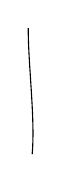
\begin{tikzpicture}[x=1cm,y=1cm,baseline=(current bounding box.south)]
\draw[line width=0.4pt] (0,0) .. controls (0.04,0.45) and (-0.05,1.12) .. (-0.05,1.60);
\end{tikzpicture}}

On suppose l'action extérieure \uline{fidèle},
i.e. $G\subset\widehat{\widehat{\mathcal T}}(\pi)
=\widehat{\widehat{\mathcal T}}$,
\inserted{et que $G=G^+$.}
On suppose de plus qu'il existe une discrétification
invariante $\pi_0$, i.e. telle que
$G\subset\mathcal T(\pi_0)$.

Si on suppose $G$ cyclique, alors sauf
erreur il est prouvé que la situation est
\uline{réalisable} topologiquement (\unsure{donc} :
\uline{\unsure{algébr.}} de façon analytique complexe $\ldots$).

\scanpage{392}
Dans le cas discret, la signification des classes de
\inserted{$\pi_0$-}conjugaison de relèvement
$G\longrightarrow\mathcal G(\pi_0)$ est bien comprise ;
\deleted{Mais}\inserted{de $\overline{\mathrm m}$ que pour les relèvements partiels}
On trouve une \deleted{\unsure{cat.} $U^{!}$} réalisation
\inserted{canonique} du groupoïde fondamental
\margin{si $U^{!}\ne\unsure{\varnothing|\phi}$}
associé au
groupe ext. $\pi_0$, par un groupoïde \inserted{fini} $[U^{!}]$
sur lequel $G$ opère au sens strict, dont les pts
correspondent aux classes de $\pi_0$-conjugaison de sections
partielles $\ne1$ maximales, le groupe
\deleted{\illegible{1}}$\mathcal T(\pi_0)^G$
opère de façon \unsure{également} canonique sur ce groupoïde.
Si $P\in U^{!}$ correspond à un relèvement
$G\longrightarrow\mathcal G(\pi_0)$, alors
un élément $\deleted{\unsure{g}}\inserted{\dot u}\in
\mathcal T(\pi_0)^G$ est dans l'image de
$\mathcal G(\pi_0)^G$, i.e. peut se remonter en
$u\in\mathcal G(\pi_0)$ commutant à $G$, sss
$\dot u(P)=P$ [i.e. sss
\inserted{(si $\dot u$ est remonté de façon \unsure{quelc.} en $v$)}
$v(G)$ est $\pi_0$-conjugué à $G$
i.e. sss $\exists g\in\pi_0$ tel que
$v(G)=\operatorname{int}(g)(G)$
i.e. \deleted{\unsure{qui}}
$u\overset{\text{déf}}{=}\operatorname{int}(g^{-1})v$ fixe $G$.
\deleted{\unsure{(Donc}} (auquel cas bien sûr il centralise,
\inserted{(par l'hyp. $\dot u\in\mathcal T^{G}$)})
Donc notre brillante assertion, est une tautologie]

\scanpage{393}
\mspage{199}
et donc le relèvement est unique. Comme
$U^{!}_{\unsure{*|\varphi}}$ est fini, donc le stabilisateur
$\mathcal T(\pi_0)^G_P$ de $P$ dans
$\mathcal T(\pi_0)^G$ est d'indice fini,
et c'est donc ce ss-groupe d'indice fini qui se remonte
gaillardement et canoniquement.

Que peut-on dire dans le contexte profini ? Bien sur,
on a une application canonique
\diagram{\begin{tikzcd}[ampersand replacement=\&,column sep=large]
\begin{gathered}
\text{\deleted{\unsure{Ens.}} classes de $\pi_0$-conj.}\\
\text{de relèvements de}\\
G\text{ en }G
\longrightarrow\mathcal G(\pi_0)\\
\text{i.e. de scindages de}\\
\text{l'ext. }1\longrightarrow\pi_0\longrightarrow
E\longrightarrow G\longrightarrow1
\end{gathered}
\arrow[r] \&
\begin{gathered}
\text{classes de $\pi_0$-}\\
\text{conj. de rel. de}\\
G\text{ en }G
\longrightarrow\widehat{\widehat{\mathcal G}}(\pi_0)\\
\text{i.e. de scindages}\\
\text{de l'extension}\\
1\longrightarrow\underset{\substack{\Vert\\\pi}}{\widehat{\pi}_0}
\longrightarrow\widehat E
\longrightarrow G\longrightarrow1
\end{gathered}
\end{tikzcd}}

Il faudrait examiner d'abord

a) La question de la bijectivité de cette appl.

b) La question si $\pi^G=1$ (\unsure{\uline{rigidité}|rigidité}),
pour $G\ne(1)$. -- (pour un relèvement donné,
dans $E$ pour simplifier)

J'ai envie de conjecturer sans vergogne
qu'il en est ainsi --- ce qui impliquerait
p.ex. que pour tt tel relèvement $G$, il y a

\scanpage{394}

un sous-groupe \uline{ouvert} \inserted{$(\unsure{\widehat{\widehat{\mathcal T}}|\widehat{\mathcal T}}^{G})_{P}$} du groupe (peut-être vraiment immense à priori !) $\widehat{\widehat{\mathcal T}}^{G}$, qui se remonte canoniquement de façon à commuter à \unsure{$\widetilde G$|$G$}....

Il faudrait manifestement faire, en $\overline{\mathrm m}$ temps qu'une théorie des op. ext. de groupes finis sur des groupes discrets à lacets (qui est pour le moment extrêmement \unsure{conjecturale|conjectural}) une théorie analogue dans le cas profini --- j'\deleted{\illegible{1}}\inserted{aurai} sans doute à y revenir par la suite.

\scanpage{395}
\mspage{200}

\uline{32} Retour sur les aspects arithmétiques du bouchage de trous : relations entre $\Gamma_{g,\nu}$ et $\Gamma_{g,\nu-1}$.

Bien sûr, on \deleted{\unsure{voit que}} a que
\[
\mathcal N_{g,\nu}\longrightarrow\mathfrak S_{\nu}
\]
est surjectif \inserted{(puisque $\mathcal T_{g,\nu}\longrightarrow\mathfrak S_{\nu}$ l'est)}, donc on aura
\[
(1)\qquad 1\unsure{\longrightarrow|-}\mathcal N_{g,\nu}^{!}\unsure{\longrightarrow|-}\mathcal N_{g,\nu}\unsure{\longrightarrow|-}\mathfrak S_{\nu}\unsure{\longrightarrow|-}1
\]
et le diagramme cartésien de \unsure{ssgroupes} de $\widehat{\widehat{\mathcal T}}_{g,\nu}$
\[
(2)\qquad
\diagram{\begin{tikzcd}[ampersand replacement=\&]
\widehat{\mathcal T}_{g,\nu}^{+}\arrow[r,hook] \& \mathcal N_{g,\nu}\\
\widehat{\mathcal T}_{g,\nu}^{!+}\arrow[u,hook]\arrow[r,hook] \& \mathcal N_{g,\nu}^{!}\arrow[u,hook]
\end{tikzcd}}
\]
\margin{\deleted{\illegible{1}} $\mathcal N_{g,\nu}=\mathcal N_{g,\nu}^{!}\cdot\widehat{\mathcal T}_{g,\nu}^{+}$ i.e. $\mathcal N_{g,\nu}$ connu par $\mathcal N_{g,\nu}^{!}$}
donnera un isomorphisme
\[
(3)\qquad \mathcal N_{g,\nu}^{!}/\widehat{\mathcal T}_{g,\nu}^{!+}\xrightarrow{\sim}\mathcal N_{g,\nu}/\widehat{\mathcal T}_{g,\nu}^{+}=\mathbb{\Gamma}_{g,\nu}
\]
Dans le cas d'un $(\pi,a)$, \inserted{($\pi$ groupe ext. à lacets,} $a$ une arithmétisation), on aura de $\overline{\mathrm m}$
\[
(4)\qquad\left\{\begin{aligned}
\mathcal N_a^{!}/\widehat{\mathcal T}_a^{+}&\simeq\mathcal N_a/\widehat{\mathcal T}_a^{+}=\mathbb{\Gamma}_a.\\
\mathcal N_a&=\mathcal N_a^{!}\widehat{\mathcal T}_a^{+}
\end{aligned}\right.
\]

Considérons maintenant \deleted{une \unsure{partie}\inserted{\unsure{$i\in I=I(\pi)$}} , \illegible{3} $\unsure{(g,\nu)}$, \unsure{et un} $\pi_i'$ \illegible{2} $\unsure{I=I(\pi)}$, et soit \illegible{1}} pour $\forall i\in I$ le stabilisateur \deleted{\illegible{1}} $\mathcal N_i$ de $i$ dans $\mathcal N$, et le groupe \deleted{extérieur} \inserted{à lacets (pas ext!)} $\pi_i'$ de type $g,\nu-1$, déduit de $\pi$ par ``bouchage du trou $i$'',
\margin{On écrit $\mathcal N$ etc. au lieu de $\mathcal N_a$. On suppose \illegible{2} $(g,\nu-1)$, i.e. \unsure{$2g-2+\nu$} \illegible{1} \unsure{$\geq1$}, i.e. $2g+\nu\geq4$}

\scanpage{396}

on a alors, pour une discrétification choisie, \deleted{\unsure{une}} \inserted{$\alpha$} compatible avec l'arithmétisation, un \unsure{hom.|hom} injectif
\[
(5)\qquad \pi_i'\xrightarrow{\varphi_i}\widehat{\mathcal T}_{\unsure{i|a}}^{+!}\subset\mathcal N_{\unsure{i|a}}^{!}\subset\widehat{\widehat{\mathcal T}}_i
\]

\deleted{On \unsure{ne peut} \illegible{2}}
\deleted{On aura}
\deleted{\unsure{qui remonte le composé}}
\deleted{\textcircled{\unsure{e|c}} L'image de $\pi'$}
tel que le composé
\[
\diagram{\begin{tikzcd}[ampersand replacement=\&]
\pi_i'\arrow[r] \& \widehat{\widehat{\mathcal T}}_i\arrow[r] \& \widehat{\widehat{\mathcal G}}(\pi_i')\\
\&\& \pi_i'\arrow[u,hook]
\end{tikzcd}}
\]
soit l'inclusion canonique. Ceci posé, on veut\margin{plutôt : \uline{il est vrai que !}} que l'image de (5) (qui n'est peut-être pas invariante dans $\widehat{\widehat{\mathcal T}}_i$) soit \uline{invariante dans \deleted{$\mathcal T$} $\mathcal N_i$}, ou ce qui revient au $\overline{\mathrm m}$, dans $\mathcal N^{!}$ (car $\mathcal N_i=\mathcal N^{!}\cdot\widehat{\mathcal T}_i^{+}$ or $\widehat{\mathcal T}_i^{+}$ invarie cette image). \deleted{\illegible{1}} Revenant à la situation universelle, cela \unsure{\uline{signifie}|signifie}
\margin{Cela signifie aussi que $\varphi_i$ \unsure{ne dépend pas} du choix de la discrétification \unsure{de donnée} $\alpha$...}

\textcircled{\unsure{e|c}} $\mathcal N_{g,\nu}^{!}\subset\widehat{\widehat{\mathcal T}}_{g,\nu}$ est contenu dans le normalisateur des $\pi_i'\hookrightarrow\widehat{\mathcal T}_{g,\nu}^{!+}$ $(0\leq i\leq\nu-1)$ \inserted{qui sont donc invariants dans $\mathcal N_{g,\nu}^{!}$} \deleted{\unsure{si} $(g,\nu-1)$ \unsure{est aussi anabélien}}.

De plus $\widehat{\widehat{\mathcal T}}_{g,\nu}^{!}\xrightarrow{\psi_i}\widehat{\widehat{\mathcal G}}_{g,\nu-1}^{!}$ induit un \deleted{\illegible{1}} \uuline{\unsure{iso|isom.}}
\[
(6)\qquad\mathcal N_{g,\nu}^{!}\xrightarrow{\sim}\mathcal M_{g,\nu-1}^{!}
\]
\margin{\uline{NB} Il suffit \unsure{me semble-t-il} de le prouver \unsure{pour un $i$} pour le déduire pour les autres \deleted{\illegible{1}}}
\margin{\uline{NB} \illegible{4}}

\scanpage{397}
\mspage{201}

Cette assertion se décompose en deux : \unsure{donc|tout} d'abord que $\psi_i$ applique bien $\mathcal N_{g,\nu}^{!}$ dans $\mathcal M_{g,\nu-1}^{!}$ -- et ceci résulte de la définition \unsure{arithmético-géom} de ces groupes -- cela implique d'autre part, puisque $\psi_i$ induit aussi un \inserted{\unsure{iso}} \deleted{\illegible{1}}
\[
\widehat{\mathcal T}_{g,\nu}^{+}
\xrightarrow{\sim}
\widehat{\mathcal G}_{g,\nu-1}^{+},
\]
qu'il induit un hom
\[
(7)\qquad
\begin{array}{ccc}
\mathbb{\Gamma}_{g,\nu}
&\xrightarrow{\substack{\inserted{\lambda_i}\\\deleted{\unsure{\psi_i}}}}&
\mathbb{\Gamma}_{g,\nu-1}\\
\wr\vert&&\wr\vert\\
\mathcal N_{g,\nu}/\widehat{\mathcal T}_{g,\nu}^{+}
&&\mathcal M_{g,\nu-1}/\unsure{\widehat{\mathcal G}}
\end{array}
\]
\deleted{et par voie \unsure{arithmétique}}
et l'inj. (resp. \deleted{b}\unsure{surjectivité}) de (6) équivaut à celle de (7). D'ailleurs (7) s'insère, par construction, dans un diagramme commutatif

(8)\quad\diagram{\begin{tikzcd}[ampersand replacement=\&,column sep=large,row sep=large]
\& \mathbb{\Gamma}_{\mathbb Q}
  \arrow[dl,"\Theta_{g,\nu}"']
  \arrow[dr,"\Theta_{g,\nu-1}"] \& \\
\mathbb{\Gamma}_{g,\nu} \arrow[rr]
\&\&\mathbb{\Gamma}_{g,\nu-1}
\end{tikzcd}}

avec $\Theta_{g,\nu}$ et $\Theta_{g,\nu-1}$ surjectifs, donc il est bel et bien évident que (6) est \uline{surjectif}. La bijectivité \unsure{\uline{signifie}|signifie} que $\Theta_{g,\nu}$ et $\Theta_{g,\nu-1}$ ont $\overline{\mathrm m}$ noyau (alors qu'à priori il se pourrait que $\Theta_{g,\nu}$ ait un noyau plus petit i.e. corresponde à une représentation de $\mathbb{\Gamma}_{\mathbb Q}$ ``moins infidèle'' que $\Theta_{g,\nu-1}$. D'ailleurs,

\scanpage{398}

il est évident \deleted{que} ($\unsure{\overline{\mathrm m}}$, à priori, sans utiliser la définition \inserted{ailleurs} \unsure{explicite|explicitée} des $\mathcal N_{g,\nu}$) que l'hom $\deleted{\unsure{\psi_i}}\inserted{\unsure{\lambda_i}}$ \inserted{\unsure{(7)}} ne dépend pas du choix de $0\leq i\leq\nu-1$ -- p.ex. puisque l'on passe de l'un à l'autre en appliquant des opérations de $\widehat{\mathcal T}^{+}$ (puisque $\widehat{\mathcal T}^{+}$ opère \unsure{transitivement} sur $I$) et que $\widehat{\mathcal T}^{+}$ opère \unsure{trivialt|trivialement} dans $\mathbb{\Gamma}_{g,\nu}$ ...

On peut dire que (6) décrit $\mathcal M_{g,\nu-1}^{!}$ (donc $\mathcal N_{g,\nu-1}^{!}$) en termes de $\mathcal N_{g,\nu}$ -- mais l'inverse est moins clair, faute de savoir si
\[
\unsure{\widehat{\widehat{\mathcal T}}_{g,\nu}^{!}}
\xrightarrow{\psi_i}
\widehat{\widehat{\mathcal G}}_{g,\nu-1}
\]
est injectif ; si on le savait, on pourrait décrire $\mathcal N_{g,\nu}^{!}$ comme l'image inverse de $\mathcal M_{g,\nu-1}^{!}$ ... \deleted{\unsure{Alors}} Il ne serait pas impossible d'ailleurs que (f) soit faux, i.e. que \inserted{les} $\Theta_{g,\nu}$ soient infidèles, mais de moins en moins quand on fait augmenter $\nu$ -- en passant à la limite \inserted{\unsure{projective}} $\Theta_{g,\infty}$, \unsure{seulement}, aurait-on

\scanpage{399}
\mspage{202}

(peut-être !) une représentation fidèle de $\mathbb{\Gamma}_{\mathbb Q}$. Mais jusqu'à indication contraire, je préfère travailler hypothétiquement avec (f), ce qui s'exprime par les suites \unsure{exactes|ex.tes} fondamentales
\[
(9)\qquad
1\longrightarrow\widehat{\pi}_{g,\nu-1}
\xrightarrow{\varphi_i}
\unsure{\mathcal N_{g,\nu}^{!}|\mathcal M_{g,\nu}^{!}}
\unsure{\overset{\psi_i'}{\longleftrightarrow}|\xrightarrow{\psi_i'}}
\unsure{\mathcal N_{g,\nu-1}^{!}|\mathcal M_{g,\nu-1}^{!}}
\longrightarrow1
\]
\margin{\unsure{\&} on pourrait l'inclure dans une suite \unsure{ex.te} un peu plus grande, avec $(\mathcal N_{g,\nu})_i$ et $\mathcal N_{g,\nu-1}$ ...}
qui étend la suite \unsure{ex.te|exacte}
\[
(10)\qquad
1\longrightarrow\widehat{\pi}_{g,\nu-1}
\xrightarrow{\varphi_i}
\widehat{\mathcal T}_{g,\nu}^{!}
\xrightarrow{\psi_i'}
\widehat{\mathcal T}_{g,\nu-1}^{!}
\longrightarrow1
\]
(et tient lieu de la suite \unsure{exacte|ex.te} peut-être défaillante
\[
??\qquad
1\longrightarrow\widehat{\pi}_{g,\nu-1}
\longrightarrow\widehat{\widehat{\mathcal T}}_{g,\nu}^{!}
\longrightarrow\widehat{\widehat{\mathcal T}}_{g,\nu-1}^{!}
\longrightarrow1
\qquad??
\]
)

Quand $(\pi,a)$ est un groupe extérieur à lacets muni d'une arithmétisation -- ce qu'on pourrait appeler une ``courbe algébrique virtuelle'' -- alors ce qui précède permet de définir, sur \inserted{chacun} des $\pi_i'$ de type $(g,\nu-1)$ associés aux $i\in I(\pi)$, \unsure{une} arithmétisation canoniquement associée à $a$, soit $\unsure{a'}$,

\scanpage{400}

et on trouve \unsure{alors|donc} une suite \unsure{exacte|exact}
\[
1 \longrightarrow \pi'_i \longrightarrow (\mathcal{N}_a)_i
\xrightarrow{\psi_i} \mathcal{N}_{a'_i} \longrightarrow 1
\tag{11}
\]
telle que l'on ait
\[
(\widehat{\mathcal{T}}^{+}_a)_i
=\psi_i^{-1}(\widehat{\mathcal{T}}^{+}_{a'_i}),
\tag{12}
\]
\[
\downarrow
\]
induisant

\diagram{\begin{tikzcd}[ampersand replacement=\&,column sep=1.9em,row sep=1.8em]
(11') \& 1 \arrow[r,dash] \& \pi'_i \arrow[r,dash] \& \mathcal N_{\unsure{a}}^{!} \arrow[r,dash,"\psi_i^{!}"] \arrow[d,phantom,"\cup" description] \& \mathcal N_{a'_i}^{!} \arrow[r,dash] \arrow[d,phantom,"\cup" description] \& 1 \\
\& \& \& \widehat{\mathcal T}_{a}^{+!} \arrow[d,phantom,"\Vert" description] \& \widehat{\mathcal T}_{a'_i}^{+!} \& \\
\& \& \& \psi_i^{\unsure{\prime}-1}\bigl(\widehat{\mathcal T}_{a_i}^{+!} \& \&
\end{tikzcd}}

et induisant par passage aux quotients
\[
\mathbb{\Gamma}_a\xrightarrow{\sim}
\mathbb{\Gamma}_{\unsure{a_i}}
\tag{13}
\]
De plus, \uline{\unsure{l'application}} canonique
\[
\unsure{\mathrm{Discrt}|\mathrm{Discr}}^{+}(\pi)\longrightarrow
\unsure{\mathrm{Discrt}|\mathrm{Discr}}^{+}(\pi'_i)
\]
définit par passage aux quotients
\[
\mathbb{P}_a\xrightarrow{\sim}\mathbb{P}_{\unsure{a_i}}
\tag{14}
\]
compatible avec les actions de $\mathbb{\Gamma}_a$,
$\mathbb{\Gamma}_{a'_i}$ et (13).

Je ne fais \inserted{ici} aucune assertion sur
une \unsure{soit-disante|soi-disante} bijectivité entre
ens. des arithmétisations de $\pi$, et \unsure{ens} des
\scanpage{401}
\mspage{203}

\unsure{arithmétisations|arithmétisation} de $\pi'_i$ --- ce qui
reviendrait à la bijectivité de
\[
\widehat{\widehat{\mathcal T}}/\mathcal N_a
\longrightarrow
\widehat{\widehat{\mathcal G}}'/\unsure{M_{a'}^{\natural}|M_{a'}^{\sharp}}
\simeq \widehat{\widehat{\mathcal T}}'/\mathcal N_{a'},
\]
qui n'a\inserted{urait} guère de raison d'être que si
on admettait
$\widehat{\widehat{\mathcal T}}(\pi)\xrightarrow{\sim}\unsure{\widehat{\widehat{\mathcal G}}|\widehat{\mathcal G}}(\pi'_i)$,
qui me semble bien problématique.

\margin{\figure{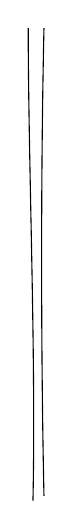
\begin{tikzpicture}[x=1cm,y=1cm,baseline=(current bounding box.north)]
\draw[line width=0.4pt] (0,0) .. controls (0.04,1.85) and (-0.06,4.30) .. (-0.06,6.00);
\draw[line width=0.4pt] (0.14,0.06) .. controls (0.10,1.90) and (0.10,4.25) .. (0.14,6.00);
\end{tikzpicture}}}
Cependant, on trouve, par le foncteur
"bouchage des trous", une équivalence
entre la catégorie des \deleted{\unsure{courbes alg.}}
groupes profinis à lacets \uuline{extérieurs} \uline{arithmétisés},
\inserted{de type $(g,\nu)$,}
et des groupes profinis à lacets
(pas extérieurs !) \uline{arithmétisés}, de type
$(g,\nu-1)$.

On peut se proposer d'essayer de
préciser \deleted{\unsure{par}} le type des propriétés
qui vont caractériser $\mathcal N_{g,\nu}$ dans $\mathcal N'_{g,\nu}=$
$\operatorname{Norm}_{\widehat{\widehat{\mathcal T}}_{g,\nu}}
(\widehat{\mathcal T}_{g,\nu}^{+})$,
\deleted{Je \unsure{pense} qu'il}
\inserted{\deleted{\unsure{On aura}}ou encore}
$\mathbb{\Gamma}_{g,\nu}$
\deleted{\unsure{pour} \illegible{1} $\Gamma'$}
dans $\mathbb{\Gamma}'_{g,\nu}=\mathcal N'_{g,\nu}/\widehat{\mathcal T}_{g,\nu}^{+}$.
On a des hom. naturels

\margin{400}

\scanpage{402}

\[
\tag{15}
\left|
\begin{aligned}
\mathbb{\Gamma}'_{g,\nu}&\longrightarrow\operatorname{Autext}(\widehat{\mathcal T}_{g,\nu}^{+})\\
\mathbb{\Gamma}'_{g,\nu}&\longrightarrow\operatorname{Aut\,ext}(\widehat{\mathcal T}_{g,\nu}^{+!})
\end{aligned}
\right.
\]
et je présume qu'\deleted{il s'agit} $\mathbb{\Gamma}_{g,\nu}$ pourra
se décrire comme image inverse d'un
sous-groupe fermé convenable de l'un
ou l'autre des seconds mbs, i.e. qu'on
peut le décrire en termes \unsure{des|de} propriétés
d'opérations extérieures sur $\widehat{\mathcal T}_{g,\nu}^{+}$ ou
sur $\widehat{\mathcal T}_{g,\nu}$. Les conditions \textcircled{e} en tous
cas sont bien de ce type (\unsure{propriété|propriétés}
de normaliser des \unsure{ss-groupes} \unsure{invariants|inscrits}
\deleted{$\unsure{\mathcal T'_i}$} $\pi'_i$ de $\mathcal T_{g,\nu}^{+!}$ ...).
Bien sûr, on
pourrait poser des conditions sur des
\unsure{automs} extérieurs (de $\widehat{\mathcal T}'{}_{g,\nu}^{+!}$, disons),
qui soient stables par passage \inserted{successifs} à des
$\widehat{\mathcal T}'{}_{g,\nu-1}^{+!}$, $\widehat{\mathcal T}'{}_{g,\unsure{\nu-2}}^{+!}$ etc ... et
\deleted{pour lesquelles}\inserted{qui soient}
engendrées par les conditions \textcircled{e}. Mais
il n'est pas dit du tout que cela

\margin{401}

\scanpage{403}
\mspage{204}

\unsure{suffira|suffise} à décrire les \deleted{$\unsure{\mathcal N_{g,\nu}}$}
$\mathbb{\Gamma}_{g,\nu}\subset\Gamma'_{g,\nu}$,
ne serait-ce que parce que la condition
devient vide pour \deleted{$\unsure{\nu=0}$} le cas limite $\nu=0$
(si $g\geq2$; ou pour les cas $g=1$, $\nu=1$, ou $g=0$, $\nu=3$).

Il est possible qu'il faille faire
intervenir des propriétés des $\pi_1$ des
$\unsure{M_{g,\nu\,\overline{\mathbb Q}_a}}$, liés à la compactification.
Ce n'est guère que dans le cas de
$(g,\nu)=(0,3)$ qu'il ne faut pas s'attendre
du tout à ce genre de conditions.

Appelons "\unsure{courbe algébrique potentielle|courbes algébriques potentielles}"
(sous-entendu, sur une clôture alg. pas précisée de $\mathbb Q$,)
la donnée d'\unsure{une|un} \inserted{\unsure{groupe} ext profini}
$\pi$ à \unsure{lacets|lacet} \deleted{profini}\inserted{\deleted{ext}}
de type $(g,\nu)$, muni d'une arithmétisation
$a$, et d'un germe de relèvement
"admissible"
\margin{\deleted{\illegible{1}}}
\[
\tag{16}
\mathbb{\Gamma}_{\unsure{a|\bullet}}^{\natural}
\longrightarrow\mathcal N_a.
\]
Elles forment une catégorie (pour les
iso, pour le moment) Si on se
donne un torseur $P$ sous $\mathbb{\Gamma}_{g,\nu}$
(ce qui \inserted{\unsure{trivialt.|moralt.}} revient à se donner une clôture

\margin{402}

\scanpage{404}
alg. $\overline{\mathbb Q}$ de $\mathbb Q$ \ldots) les courbes potentielles
de type $(g,\nu)$ \uline{\unsure{relatifs|relatives}} à ce torseur
(\unsure{moralt|moralmt}, \unsure{correspondant|correspondent} à des courbes
alg. sur $\overline{\mathbb Q}$ \ldots) sont \inserted{celles} munies en
plus d'un \unsure{isom.} (``intérieur'')
\[
(17)\qquad \mathbb P_a\xrightarrow{\sim}P
\]
(définissant un isomorphisme
\[
(18)\qquad \mathbb{\Gamma}_a\longrightarrow\Gamma_P
 =\operatorname{Aut}_{\mathbb{\Gamma}_{g,\nu}}(P).
\]
\margin{Le cas où $P$ est le torseur
trivial, est celui des \deleted{\unsure{courbes}} $\pi$ ext \unsure{(?)|(18)}
munis d'une \uline{prédiscrétification} orientée $\alpha$
(d'où une \deleted{\illegible{1}} \unsure{suite} exacte
$1\longrightarrow\widehat{\mathcal T}_\alpha\longrightarrow
\mathcal N_\alpha\longrightarrow\mathbb{\Gamma}_\alpha\longrightarrow1$)}

Cette fois-ci, on s'attend à trouver
des \unsure{ens} d'iso. \uline{finis}, au lieu de
torseurs sous des groupes profinis
considérables.

On considère les \deleted{\unsure{P}} \uline{Points} de $\pi$,
comme les classes de \inserted{$\pi$-}conjugaison
des \unsure{relèvts} ``admissibles'' de (16),
\unsure{en|ou}
\[
(19)\qquad\mathbb{\Gamma}_{\unsure{a|\bullet}}^{\natural}\longrightarrow
\mathcal M_a\subset\widehat{\widehat{\mathcal T}}(\pi)
\]
i.e. un germe de vraie action de $\mathbb{\Gamma}_{\bullet}$
sur $\pi$, avec
\margin{(20)}
\figure{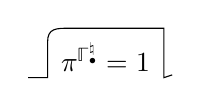
\begin{tikzpicture}[baseline=(eq.base)]
\node[inner sep=0pt,outer sep=0pt] (eq) {$\pi^{\mathbb{\Gamma}_{\bullet}^{\natural}}=1$};
\draw[line width=0.4pt]
([xshift=-12pt,yshift=-2pt]eq.south west)
-- ([xshift=-5pt,yshift=-2pt]eq.south west)
-- ([xshift=-5pt]eq.north west)
.. controls ([xshift=-5pt,yshift=5pt]eq.north west) and ([xshift=-2pt,yshift=5pt]eq.north west) .. ([xshift=3pt,yshift=5pt]eq.north west)
-- ([xshift=5pt,yshift=5pt]eq.north east)
-- ([xshift=5pt,yshift=-2pt]eq.south east)
-- ([xshift=8pt,yshift=-1pt]eq.south east);
\end{tikzpicture}}
(ceci pour \deleted{\unsure{l'ad}}
\margin{403}

\scanpage{405}
\mspage{205}
l'admissibilité.

\uline{Question liminaire} La connaissance de
$\pi$, de $\underbrace{\widehat{\mathcal T}_a^+}_{\Sigma_a}
\subset\widehat{\widehat{\mathcal T}}(\pi)$, et \unsure{d'un} ss-groupe
$\Gamma'\subset\widehat{\widehat{\mathcal T}}(\pi)$
(normalisant $\Sigma_a$, \inserted{tel que
$\Gamma'\cap\unsure{\Sigma_a|\Sigma_{\bullet}}=(1)$})
\unsure{permettrait-il} de retrouver l'\unsure{arithmatisation|arithmétisation} de $\pi$
--- et, pour commencer, de retrouver
$\mathcal N_a$ (dans lequel $\Gamma'\cdot\Sigma$ est d'indice
fini) ? \deleted{Est} Il \unsure{suffirait|suffira}, pour pouvoir
répondre par l'affirmative, de savoir
que tt \unsure{isom.} ext. $\pi\longrightarrow\pi_{g,\nu}$,
qui envoie \inserted{$\Sigma$ sur $\widehat{\mathcal T}_{g,\nu}=\Sigma_{g,\nu}$, et}
\unsure{tt|le} ss-groupe d'indice
fini $\Gamma'\cdot\Sigma$ dans $\mathcal N_a$ dans $\mathcal N_{g,\nu}$,
est compatible avec les \unsure{arithmatisations|arithmétisations}.
Or ceci revient \unsure{exactt|exactmt} :

\textcircled{g} (facultatif, quand même !)
\deleted{tout} Pour tt sous-groupe
ouvert $\mathcal N'$ de $\mathcal N_{g,\nu}$,
les éléments de $\widehat{\widehat{\mathcal T}}_{g,\nu}$
\inserted{normalisant $\widehat{\mathcal T}_{g,\nu}$ et}
qui transportent
$\mathcal N'$ dans $\mathcal N_{g,\nu}$, \unsure{sont} dans $\mathcal N_{g,\nu}$
(\unsure{a fortiori},
$\mathcal N_{g,\nu}$ serait son propre normalisateur
dans $\operatorname{Norm}_{\widehat{\widehat{\mathcal T}}_{g,\nu}}
(\widehat{\mathcal T}_{g,\nu})$.
\margin{404}

\scanpage{406}
Avec les ``points de $U$'' (définis comme \unsure{classes}
de conjugaison de \unsure{relèvts} (19)
``admissibles'' i.e. satisfaisant (20), on
fait un groupoïde, ayant comme
groupe fondamental extérieur $\pi$, et sur
lequel $\Gamma^{\unsure{\natural|\sharp}}\subset\mathcal N_a$ opère strictement
(\uline{NB} pour se reposer, on se donne
maintenant $\unsure{\Gamma^{\natural}|\Gamma}$ lui-$\overline{\mathrm m}$, pas \unsure{seulmt|seulement} un
germe --- \unsure{moralmt|moralement}, cela signifie
qu'on a une courbe définie sur une
sous-ext. finie $K$ de $\overline{\mathbb Q}/\mathbb Q$ \ldots\unsure{\}|)}.
Les pts fixes de $\Gamma$ correspondent
aux pts rat/$K$, les pts fixes sous un
ss-groupe fermé $\Gamma'$ aux pts rationnels
sur la sous-extension $K'$ de $\overline{\mathbb Q}/\mathbb Q$ asso-
ciée à $\Gamma'$ \ldots)
\margin{405}

\scanpage{407}
\mspage{206}

Soit maintenant
\figure{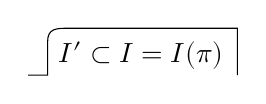
\begin{tikzpicture}[baseline=(eq.base)]
\node[inner sep=0pt,outer sep=0pt] (eq) {$I'\subset I=I(\pi)$};
\draw[line width=0.4pt]
([xshift=-11pt,yshift=-2pt]eq.south west)
-- ([xshift=-4pt,yshift=-2pt]eq.south west)
-- ([xshift=-4pt]eq.north west)
.. controls ([xshift=-4pt,yshift=5pt]eq.north west) and ([xshift=-1pt,yshift=5pt]eq.north west) .. ([xshift=4pt,yshift=5pt]eq.north west)
-- ([xshift=5pt,yshift=5pt]eq.north east)
-- ([xshift=5pt,yshift=-2pt]eq.south east);
\end{tikzpicture}}
une
partie de $I$, stable par $\Gamma$. On trouve
par "bouchage des trous en $I'$" un
groupe ext. à lacets $\pi'$, \deleted{qui} et un
hom extérieur
\[
(20)\qquad \pi^{\unsure{\natural|\sharp}}\longrightarrow\pi'
\]
D'ailleurs $\pi'$ hérite d'une arithmétisation \inserted{$a'$}
par $\pi$ -- et on aura
\[
(21)\qquad
\left\{
\begin{array}{ccc}
\mathbb{\Gamma}_a & \overset{\sim}{\longrightarrow} & \mathbb{\Gamma}_{a'} \\
\mathbb P_a & \overset{\sim}{\longrightarrow} & \mathbb P_{a'} \\
\unsure{\wr} & & \\
P & &
\end{array}
\right.
\quad\unsure{\leadsto}
\]
donc $\pi'$ est défini sur \unsure{le|la} $\overline{\mathrm m}$ $P$ que
$\mathbb{\Gamma}_a$
(i.e. en faisant des trous dans $U$ pour
trouver $U'$, on n'a pas dérangé le
corps de base alg. \unsure{clos|abs} $\overline{\mathbb Q}\ldots$). D'ailleurs
on aura un hom canonique
\[
\widehat{\mathcal T}(\pi)\longrightarrow
\widehat{\mathcal T}(\pi')
\]
induisant
\[
(22)\qquad
\]
\diagram{\begin{tikzcd}[ampersand replacement=\&,column sep=3.2em,row sep=1.8em]
\mathcal N_a \arrow[r] \arrow[d,phantom,"\cup" description] \& \mathcal N_{a'} \arrow[d,phantom,"\cup" description] \\
\widehat{\mathcal T}_a \arrow[r,dash] \& \widehat{\mathcal T}_{a'}
\end{tikzcd}}

\margin{406}

\scanpage{408}

(induisant justement $\mathbb{\Gamma}_a\longrightarrow\mathbb{\Gamma}_{a'}$ par passage
aux quotients), et on trouve, en
composant
\[
\Gamma\;\unsure{\subset|\hookrightarrow}\;\mathcal N_a\longrightarrow\mathcal N_{a'}
\]
un hom \unsure{égalmt|également} injectif
\[
(23)\qquad\Gamma\hookrightarrow\mathcal N_{a'}
\]
qui est une \unsure{quasi-section|quasi section} de $\mathcal N_{a'}$ sur $\mathbb{\Gamma}_{a'}$,
Donc \deleted{\unsure{que|par}}\inserted{sous} réserve d'admissibilité,
on trouve sur \deleted{\illegible{1}} $\unsure{\pi'|\pi}$ une structure
de courbe algébrique potentielle, relatif
au $\overline{\mathrm m}$ $P$.

\deleted{L'admissibilité s'exprime
\unsure{peut-être par} la condition
\[
(24)\qquad {\pi'}^{\Gamma}=(1)
\]
-- et s'il le faut, on mettra ces
conditions (pour \unsure{tte|$\forall$} $I'\subset I$) dans
la définition de l'admissibilité de}

\deleted{\illegible{1} \unsure{Je}} Je suis vraiment gêné
aux entournures, faute d'avoir une
définition en forme de "admissible" --

\margin{407}

\scanpage{409}
\mspage{207}

je vais y revenir très vite --- mais
pour le moment, j'ai envie de noter que,
\deleted{du fait que $\Gamma$ \unsure{opérait} \unsure{tr.}}
\inserted{si $I'\neq\varnothing$,}
le groupe ext. $\pi'$ peut se décrire par
un \inserted{vrai} groupoïde, ayant $I'$ comme ens.
d'objets, et sur lequel $\Gamma$ opère en
sens strict (ceci est de l'algèbre pure,
indépendamment des histoires d'arithmétisation\ldots)
Le fait que $\Gamma$ opère \unsure{trivialt}
sur les $i'\in I'$ implique que pour \unsure{tt|$\forall$}
$i'\in I'$, on a un \deleted{\unsure{relèvement de}}
\unsure{hom.} canonique
\[
(24)\qquad \Gamma\longrightarrow\pi'(i')
\]
qui relève son action \unsure{extérieur|extérieure}, d'où
une \unsure{uq} classe de \inserted{$\pi'$-}conj. de relèvements
de l'action ext. de $\Gamma$ sur $\pi'$
en une vraie action de $\Gamma$ sur $\pi'$
--- on espère qu'elle satisfait ${\pi'}^{\Gamma}=1$ ---
et on a donc une application can.
\[
(25)\qquad I'\longrightarrow\mathrm{Pts}(\pi',\alpha',\Gamma)
\]

\margin{408}

\scanpage{410}

Je \uline{dis que cette application est injective}

Ceci est "évident" quand on interprète
"action ext. admissible" par "réalisable
par une vraie courbe alg.", et
"relèvements admissibles" par "réalisables
par des vrais pts rat / \unsure{$K^+$|$K$}, corps des
\unsure{fixes|invariants} de $\Gamma$". Mais on voudrait
bien sûr des raisons internes à
la donnée des $(\mathcal N_{g,\nu})$, et des \unsure{)}
propriétés de ces données ! \deleted{\unsure{Et}}

\margin{On \unsure{est ramené|va revenir} au cas Card $I'=2$\ldots}

Ce pt étant admis (en mettant
entre parenthèses les deux définitions
\unsure{éventuelles|essentielles} d'admissibilité, sur lesquelles
on va revenir plus bas) on trouve
un foncteur "bouchage de trous"
\diagram{\begin{tikzcd}[ampersand replacement=\&,column sep=large]
\begin{gathered}
\text{Courbes algébriques}\\
\text{potentielles sur }P,\ \text{\unsure{\deleted{relatives}|relatives}}\\
\text{à un ss-groupe ouvert}\\
\text{\deleted{\unsure{d'un ens}}}\\
\Gamma\text{ de }\mathbb{\Gamma}_P,\ \text{et munies d'un}\\
\text{ens }I'\text{ de pts à l'}\infty
\end{gathered}
\arrow[r]
\&
\begin{gathered}
\text{Courbes alg.}\\
\text{pot. sur }P\text{ relatives}\\
\text{à }\Gamma,\ \text{munies}\\
\text{d'une partie}\\
\text{de l'ens des}\\
\text{"Pts \unsure{ratls|invts}/}\Gamma\text{"}
\end{gathered}
\end{tikzcd}}

\margin{il faut pour ceci les restrictions
anabéliennes habituelles}

\margin{409}
\scanpage{411}
\mspage{208}

et sauf erreur, il est devenu évident
que ce foncteur est une \uline{équivalence de
catégories} (et comme conséquence, il
\margin{\unsure{pour les} \uline{\unsure{isom}}}
y a le foncteur en sens inverse :
forer des trous en des ``pts'' invariants
sous $\Gamma_{\unsure{a|0}}$ (ou en des pts quelconques
quitte à passer à un $\Gamma'$ plus petit).

Mais je me rends compte que
\deleted{\illegible{1}} ce n'est pas du tout évident -- je vais
essayer d'élucider la situation axiomatiquement.
On a fixé un genre $g$,
on suppose donné, pour $\nu$ variable
(tel que $(g,\nu)$ anabélien) des
sous-groupes fermés $N_{g,\nu}\subset\widehat{\widehat{\mathcal T}}_{g,\nu}$,
normalisant $\widehat{\mathcal T}_{g,\nu}$, et satisfaisant la
condition essentielle que les $\psi_i:\widehat{\widehat{\mathcal T}}_{g,\nu}\longrightarrow\widehat{\widehat{\unsure{\mathcal G|\mathcal S}}}_{g,\nu-1}$
induisent
\[
M_{g,\nu}\xrightarrow{\sim}M_{g,\nu-1}
\]
Ce qui permet de définir la notion
d'arithmétisation d'un $\pi$ profini de
type $(g,\nu)$ anabélien, et la théorie du

\scanpage{412}

bouchage d'un nb quelc. de trous, et
du forage d'1 seul trou, dans la
catégorie des groupes de type $g,\nu$,
arithmétisés.

On suppose d'autre part \unsure{donné|donnée} une
sous-catégorie pleine de la cat. des groupes
\margin{\unsure{on la suppose} : stable par prise des ss-groupes ouverts.}
profinis (qui pourrait se réduire aux
sous-groupes ouverts de $\mathbb{\Gamma}_g$, valeur
commune des $\mathbb{\Gamma}_{g,\nu}$ ou des sous-groupes
ouverts du groupe $\mathbb{\Gamma}_a$, $a$ une
arithmétisation), et \deleted{des} \inserted{une notion d'}opérations
extérieures \inserted{``admissibles''} de tels $\Gamma$ sur les
$\pi$ arithmétisés. On suppose

\textcircled{1} Si $\Gamma$ opère admissiblement sur $\pi$, tt
sous-groupe ouvert aussi (\deleted{\unsure{et}} et inversement ?)

\textcircled{2} Si de plus $\Gamma$ invarie une partie $I'$
de $I=I(\pi)$, alors en ``bouchant $I'$'',
l'opération de $\Gamma$ sur $\pi'$ est admissible.

\margin{Il suffit de \unsure{la poser|le prouver} pour $\operatorname{card} I'=1$, i.e. bouchage \unsure{d'un|d'un seul} trou -- \unsure{du moins si on sait que la condition d'admissibilité ne dépend que de l'action des noyaux des groupes}.}

\deleted{\illegible{1}}
\deleted{\unsure{On se propose de définir une notion d'action admissible} \illegible{2}}
\inserted{Quand on a une action \inserted{\uline{effective}}, \unsure{(pas extérieure)|(non extérieure)}}
de $\Gamma$ sur un $(\pi,a)$, alors le foncteur
\unsure{de} ``\deleted{bouchage}\inserted{forage} des trous'' donne une action
ext. sur un $(\pi^0,a^0)$ de type $g,\nu+1$,
et on dit que l'action de départ est

\scanpage{413}
\mspage{209}

admissible, si l'action \uline{extérieure} déduite l'est.

On trouve ainsi une \uline{équivalence} entre
la cat. des \deleted{\unsure{cat.}} systèmes $(\pi,a,\Gamma,\psi,i)$
d'un $(\pi,a)$ de type $(g,\nu+1)$, avec une
op. \inserted{\uline{ext.}} admissible $\psi$ d'un $\Gamma$ dessus, et
un $i\in I(\pi)$ stable par $\Gamma$, avec la cat.
des $(\pi',a',\Gamma,\psi')$ des $(\pi',a')$ de type
$(g,\nu)$, avec une \uline{vraie} action admissible $\psi'$
de $\Gamma$ dessus.

\deleted{\unsure{On doit} \illegible{3}}
\inserted{La condition (1) assure que}
\deleted{\textcircled{3} \unsure{Si une vraie action}}
\inserted{si $\Gamma$ opère \deleted{\uline{\unsure{vraiment}}} \deleted{\unsure{admissible|admissiblement}} effectivement, de façon}
admissible, alors l'action extérieure déduite
est admissible (mais l'inverse ne
sera pas vrai -- il y aura des relèvements
``pathologiques'' d'une action \unsure{cat.|ext.} admissible
donnée\ldots). On suppose de plus

\margin{\figure{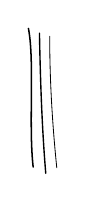
\begin{tikzpicture}[x=1cm,y=1cm,line cap=round,baseline=(current bounding box.center)]
\draw[line width=0.55pt] (0.04,1.80) .. controls (0.12,1.38) and (0.04,0.57) .. (0.10,0.04);
\draw[line width=0.50pt] (0.18,1.74) .. controls (0.19,1.20) and (0.21,0.55) .. (0.26,-0.04);
\draw[line width=0.30pt] (0.31,1.70) .. controls (0.31,1.09) and (0.35,0.52) .. (0.40,0.03);
\end{tikzpicture}}}
\textcircled{3} Si $\Gamma$ opère \inserted{effect.} de façon admissible sur
$\pi$, alors $\pi^\Gamma=(1)$.

\deleted{Soit \unsure{Alors}}
Cela implique que la catégorie des
$\Gamma$-Pts de $\pi$, ou si on veut des sections
de $B_{\pi,\Gamma}\,(\unsure{\simeq}B_u)$ sur $B_\Gamma$, est \uline{rigide}.

\scanpage{414}

Mais \deleted{\unsure{appelons|supposons}} considérons la catégorie limite inductive des \deleted{\illegible{1}} catégories des sections de $B_{\pi,\Gamma}\simeq B_u$ sur des $B_{\Gamma'}$ ($\Gamma'$ sous-groupe ouvert), elle est discrète et correspond à l'ens
\[
\mathrm{Pt}_{\mathrm{ad}}(B_{\pi,\Gamma^{\natural}})\simeq
\underset{\substack{\Gamma'\ \mathrm{ouvert}\\\mathrm{de}\ \Gamma}}{\varinjlim}
\mathrm{Pt}_{\mathrm{ad}}(B_{\pi,\Gamma'}).
\]

\margin{\uline{NB} Le gr.-poïde à opérateurs stricts $\uline{\mathrm{Pt}}(B_{\pi,\Gamma})$ dépend \unsure{fonctoriellement} de $(\pi,\Gamma)$, \illegible{1} pour des morphismes ext. \deleted{\unsure{dans}} \unsure{plus} \illegible{3} de $\Gamma$, si \deleted{\illegible{4}}.}

\deleted{\textcircled{4} \unsure{Pour} \illegible{2} $\mathrm{Pt}(B_{\pi,\Gamma})$ \illegible{1}. D'autre part, $\pi$ peut être défini par un groupoïde.}
Si $\mathrm{Pt}(B_{\pi,\Gamma})\ne\varnothing$, alors (du seul fait que $\pi^{\Gamma'}=(1)$ pour $\forall$ sous-groupe ouvert de $\unsure{\Gamma'|\Gamma}$) \inserted{le gr. cat.} $\pi$ peut être décrit \unsure{can.|com.} par un groupoïde \inserted{profini $\uline{\mathrm{Pt}}(B_{\pi,\Gamma^{\natural}})$} ayant $\mathrm{Pt}(B_{\pi,\Gamma})$ comme ens d'objet, \deleted{\unsure{et|alors}} \inserted{\unsure{lié|liés} par le groupe cat. $\pi$, sur} lequel $\Gamma$ opère en sens strict, avec le stabilisateur \inserted{$\Gamma_P$} de $\forall$ pt étant ouvert. et $\Gamma_P\to\mathrm{Aut}(P)$ $(\simeq\pi\ \text{mod \unsure{autom. int.}})$

\deleted{De façon plus précise, \unsure{indépendamment de} l'axiomatique précédente, on peut décrire les syst. \unsure{formés} d'un groupe \inserted{cat. $\pi$} profini, et d'une opération \inserted{ext.} \unsure{d'un groupe profini} $\Gamma$ dessus, \unsure{satisfaisant}}

étant continue. On a ici \unsure{si} à $\forall\ P\in\mathrm{Pt}(B_{\pi,\Gamma})$ on associe la classe d'isom. de \deleted{\unsure{groupes de relèvements}}

\scanpage{415}
\mspage{210}

\deleted{\unsure{groupes}} de sections de $B_{\pi,\Gamma}$ sur $B_\Gamma$, on trouve une bijection -- ce qui caractérise le \inserted{$\Gamma$-}groupoïde en question à \uline{isom} unique près. On suppose

\textcircled{4} Si $\Gamma$ opère admissiblement sur $(\pi,a)$, alors il existe un sous-groupe ouvert $\Gamma'$ de $\Gamma$ \deleted{peut \unsure{opérer de façon}} \inserted{dont l'op. \inserted{cat.} se relève en une} op. effective admissible -- i.e. $\mathrm{Pt}_{\mathrm{ad}}(B_{\Gamma,\pi})\ne\varnothing$.

\deleted{Ceci dit, considérons \deleted{\illegible{1}} la situation d'une action \inserted{ext.} admissible de $\Gamma$ sur $(\pi,a)$ et d'un $i\in I(\pi)$ \deleted{stable} fixe sous $\Gamma$. On a donc une action \uline{effective} \inserted{\unsure{admiss.}} de $\Gamma$ sur $(\pi',a')$, \deleted{et de plus on a} \inserted{donc une action extérieure,} plus un Pt ``$\Gamma$-rationnel'', i.e. invariant sous $\Gamma$. Considérons d'autre part un \unsure{relèvement} admissible $\Gamma\longrightarrow M(\pi,a)$, et \illegible{2}}

Notons que dans la situation envisagée, du bouchage d'un trou $i\in I(\pi)$ d'un $\pi$, en plus de l'hom.
\[
\widehat{\widehat{\mathcal T}}(\pi)_i
\xrightarrow{\psi_i}
\widehat{\widehat{\unsure{\mathcal G|\mathcal S}}}(\pi'_i)
\]
associé, donnant par composition
\[
\widehat{\widehat{\mathcal T}}(\pi)_i
\xrightarrow{\psi'_i}
\widehat{\widehat{\mathcal T}}(\pi'_i)
\]

\scanpage{416}

d'où une action extérieure de $\widehat{\widehat{\mathcal T}}(\pi)$ sur $\pi'_i$, \inserted{\unsure{de façon} \unsure{que les} $\pi\overset{p_i}{\longrightarrow}\pi'_i$ \unsure{commutent|commutant} aux act. ext. de $\widehat{\widehat{\mathcal T}}(\pi)$, \deleted{\illegible{1}}} on a un homomorphisme canonique d'extensions, \deleted{associé} provenant de cette action extérieure et de l'hom. $p_i:\pi\longrightarrow\pi'_i$,

\diagram{\begin{tikzcd}[ampersand replacement=\&,column sep=2.4em,row sep=3.4em,
execute at end picture={
  \path (\tikzcdmatrixname-1-4.south west) -- (\tikzcdmatrixname-2-3.north east) coordinate[pos=.5] (lmfixnineteendiag);
  \draw[line width=.35pt] ([xshift=-5mm,yshift=1mm]lmfixnineteendiag) -- ([xshift=-6mm,yshift=1mm]lmfixnineteendiag) -- ([xshift=-6mm,yshift=-5mm]lmfixnineteendiag) -- ([xshift=-5mm,yshift=-5mm]lmfixnineteendiag);
  \draw[line width=.35pt] ([xshift=8mm,yshift=5mm]lmfixnineteendiag) -- ([xshift=9mm,yshift=5mm]lmfixnineteendiag) -- ([xshift=9mm,yshift=-1mm]lmfixnineteendiag) -- ([xshift=8mm,yshift=-1mm]lmfixnineteendiag);
}]
1 \arrow[r,dash] \& \pi \arrow[r,dash] \arrow[d,"p_i"] \&
\widehat{\widehat{\unsure{\mathcal G|\mathcal S}}}(\pi)_i \arrow[r] \arrow[d,"\varphi_i"] \&
\widehat{\widehat{\mathcal T}}(\pi)_i \arrow[r,dash] \arrow[d,"\psi'_i"] \arrow[dl,dashed,"\psi_i"'] \& 1 \\
1 \arrow[r,dash] \& \pi'_i \arrow[r] \&
\widehat{\widehat{\unsure{\mathcal G|\mathcal S}}}(\pi'_i) \arrow[r,dash] \&
\widehat{\widehat{\mathcal T}}(\pi'_i) \arrow[r,dash] \& 1
\end{tikzcd}}

qui n'est pas la \unsure{composée|composé}
\[
\widehat{\widehat{\unsure{\mathcal G|\mathcal S}}}(\pi)_i
\longrightarrow\widehat{\widehat{\mathcal T}}(\pi)_i
\xrightarrow{\psi_i}\widehat{\widehat{\unsure{\mathcal G|\mathcal S}}}(\pi'_i).
\]
(il peut se définir chaque fois qu'on a un groupe $\Gamma$, ici $\widehat{\widehat{\mathcal T}}(\pi)$, qui \deleted{\unsure{de centre trivial}} \inserted{\unsure{commutant|commute}} extérieurement sur deux groupes ext $\pi,\pi'$, et qu'on a un hom \inserted{$\unsure{\beta|p}$} \deleted{\illegible{1}} $\pi\longrightarrow\pi'$ qui commute à l'action de $\Gamma$, et tel que le \inserted{centre de $\pi$ et \unsure{le|les}} \unsure{centralisateur|centralisateurs} de \unsure{son image|$\beta(\pi)$} dans $\pi'$ soient triviaux\ldots)
\inserted{\unsure{C'est aussi ici} l'hom de ``transport de str.''}, \inserted{qui} \unsure{pour} \unsure{tout|\deleted{tout}} autom. à lacets $u$ de $\pi$, associe l'autom. \unsure{corresp.|canonq.} de $\pi'_i$.

On \unsure{a\deleted{vait}|\deleted{avait}} oublié de préciser :

\textcircled{\unsure{g|9}} L'hom canonique $(\widehat{\widehat{\unsure{\mathcal G|\mathcal S}}}_{g,\nu})_i\longrightarrow\widehat{\widehat{\unsure{\mathcal G|\mathcal S}}}_{g,\nu-1}$ associé à $i\in[0,\nu-1]$, envoie $(M_{g,\nu})_i$ dans $M_{g,\nu-1}$ \deleted{dans} donc il s'insère dans un \unsure{hom.|diagr.} de suites exactes

\scanpage{417}
\mspage{211}

(26)
\diagram{
\begin{tikzcd}[ampersand replacement=\&]
1 \arrow[r,dash] \& \pi \arrow[r,dash] \arrow[d] \&
M_a(\pi)_i \arrow[r] \arrow[d, "\varphi_i"']
\arrow[dr, phantom, "{\text{\unsure{\uline{non}|\uline{pas}} \unsure{comm.?}}}" description, near start] \&
N_a(\pi)_i \arrow[r] \arrow[d, "\text{\unsure{comm.}}"'] \arrow[dl, dashed] \& 1 \\
1 \arrow[r,dash] \& \pi'_i \arrow[r] \&
M_{a'}(\pi'_i) \arrow[r,dash] \& N_{a'}(\pi'_i) \arrow[r,dash] \& 1
\end{tikzcd}
\par [Les segments horizontaux issus des deux $1$ de gauche n'ont pas de pointe visible. Les extrémités droites des segments $\pi$--$M_a(\pi)_i$ en haut, $M_{a'}(\pi'_i)$--$N_{a'}(\pi'_i)$ et $N_{a'}(\pi'_i)$--$1$ en bas sont épaissies, sans pointe lisible avec certitude. Une tache d'encre (surcharge) suit la parenthèse de $M_a(\pi)_i$. Le mot \unsure{comm.} est écrit dans le triangle de droite, entre la flèche pointillée et la flèche verticale de droite ; ce n'est pas une étiquette lisible de la flèche pointillée.]
}.

Ceci posé, si on a une opération \inserted{ext} admissible
$\Gamma\longrightarrow N_a(\pi)$ de $\Gamma$ sur $\pi$,
\inserted{fixant $i$,} donc aussi par
$N_a(\pi)\longrightarrow N_{a'}(\pi'_i)$ sur $\pi'_i$,
on peut considérer que \unsure{\deleted{tout}} relèvement
$\Gamma\longrightarrow M_a(\pi)$ \inserted{pour $\pi$} définit
par composition un relèvement $\Gamma\longrightarrow M_{a'}(\pi'_i)$
pour $\pi'_i$. \deleted{Dire que}
\inserted{On conclut aisément de}
\textcircled{2} que si le premier est admissible, le deuxième l'est.
On trouve donc
\[
(27)\qquad
\mathrm{Pt}_{\mathrm{ad}}(B_{\pi,\Gamma})
\longrightarrow
\mathrm{Pt}_{\mathrm{ad}}(B_{\pi'_i,\Gamma})
\]
(et en passant à la limite, une application de $\Gamma$-ensembles
\[
(28)\qquad
\mathrm{Pt}_{\mathrm{ad}}(B_{\pi,\Gamma^{\natural}})
\longrightarrow
\mathrm{Pt}_{\mathrm{ad}}(B_{\pi'_i,\Gamma^{\natural}})
\]
-- qui correspond d'ailleurs à un hom. de \unsure{$\Gamma$} groupoïdes
\[
(29)\qquad
\uline{\mathrm{Pt}}_{\mathrm{ad}}(B_{\pi,\Gamma^{\natural}})
\longrightarrow
\uline{\mathrm{Pt}}_{\mathrm{ad}}(B_{\pi'_i,\Gamma^{\natural}}).
\]

Ceci posé, soit $P\in\mathrm{Pt}_{\mathrm{ad}}(B_{\pi'_i,\Gamma})$
le ``pt canonique'' de
$\mathrm{Pt}_{\mathrm{ad}}B_{\pi'_i,\Gamma}
=\bigl(\mathrm{Pt}_{\mathrm{ad}}(B_{\pi'_i,\Gamma^{\natural}})\bigr)^\Gamma$.

\scanpage{418}

On demande :

\textcircled{5} L'application (27) induit une \uline{bijection}\unsure{.}
\figure{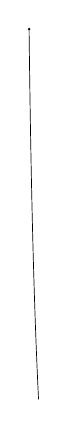
\begin{tikzpicture}[x=1mm,y=1mm,baseline=(current bounding box.north)]
\fill (0,0) circle[radius=.18mm];
\draw[line width=.25pt,line cap=round] (0,-.2) .. controls (.15,-13) and (.45,-32) .. (1.2,-47);
\end{tikzpicture}}
\[
\mathrm{Pt}_{\mathrm{ad}}(B_{\pi,\Gamma})
\longrightarrow
\mathrm{Pt}_{\mathrm{ad}}(B_{\pi'_i,\Gamma})\setminus\{P\}
\]
ou encore (passant à la limite) une bijection de $\Gamma$-ensembles
\[
\mathrm{Pt}_{\mathrm{ad}}(B_{\pi,\Gamma^{\natural}})
\simeq
\mathrm{Pt}_{\mathrm{ad}}(B_{\pi'_i,\Gamma^{\natural}})\setminus\{P\}
\]

Ceci signifie trois choses :

a) L'hom canonique $\Gamma\longrightarrow M_{a'}(\pi'_i)$,
composé de $\Gamma\longrightarrow N_a(\pi)$ et de
$N_a(\pi)\simeq M_{a'}(\pi'_i)$,
n'est pas \inserted{$\pi'_i$-}conjugué à un hom composé
$\Gamma\xrightarrow{\lambda}M_a(\pi)
\xrightarrow{\varphi_i}M_{a'}(\pi'_i)$,
où $\Gamma\xrightarrow{\lambda}M_a(\pi)$ est un relèvement admissible.

b) Si $\lambda,\mu:\Gamma\rightrightarrows M_a(\pi)$ sont deux
relèvements admissibles de $\Gamma\longrightarrow N_a(\pi)$
\deleted{\unsure{que}} tels que
$\varphi_i\circ\lambda$ et $\varphi_i\circ\mu:
\Gamma\rightrightarrows M_a(\pi)$ soient
\inserted{$\pi'_i$-}conjugués, alors $\lambda$ et $\mu$ sont déjà
\inserted{$\pi$-}conjugués.

c) Tout relèvement admissible de
$\Gamma\longrightarrow N_{a'}(\pi'_i)$ en
$\Gamma\longrightarrow M_{a'}(\pi'_i)$,
provient par composition d'un rel. admissible
$\Gamma\longrightarrow M_a(\pi)$.

\scanpage{419}
\mspage{212}

Grâce à ceci, l'équivalence de catégories entre systèmes
$(\pi,a,i,\Gamma,\unsure{\theta}:\Gamma\mathop{\longrightarrow}\limits_{\unsure{\mathrm{adm}}}\unsure{N_a})$,
et les systèmes $(\pi',a',\Gamma,\theta':\Gamma\longrightarrow\unsure{N_{a'}},P)$,
où $P\in\mathrm{Pt}(B_{\pi',\Gamma^{\natural}})^\Gamma$,
se précise de façon parfaite au niveau des points: les
Points $\Gamma$-rationnels de $B_{\pi\unsure{,\Gamma^{\natural}|\deleted{,\Gamma^{\natural}}}}$
s'identifient à \unsure{l'un|l'ens}
\deleted{des pts $\Gamma$-\unsure{rationnels}} des pts $\Gamma$-rationnels
de $B_{\pi'}$, distincts de $P$.

Ceci nous permet alors (ce qui n'était pas faisable dans le contexte
discret!) d'étendre l'équivalence de catégories en une équivalence

\[
(30)\qquad
\begin{array}{c@{\quad}c@{\quad}c}
\parbox[t]{0.45\linewidth}{%
cat. des systèmes $(\pi,\unsure{a|\alpha},I',\Gamma,\theta:\Gamma\longrightarrow N_a)$
d'un $\pi$ arithmétisé \inserted{(par \unsure{$\alpha$|$a$})} de type $(g,\nu)$,
de $I'\subset I(\pi)$, d'une action
\uline{admissible} ext. de $\Gamma$ sur $\pi$
telle que $\Gamma$ \deleted{\unsure{op.}} \uline{fixe chaque point} de $I'$
}
& \unsure{\cong|\simeq} &
\parbox[t]{0.36\linewidth}{%
cat des syst.
$(\pi',\unsure{a'|\alpha'},I',\unsure{\Gamma^{*}|\Gamma},\theta':\Gamma\longrightarrow N_{a'})$
d'un $\pi'$ arithmétisé (par \unsure{$a'$|$\alpha'$}) de type
$(g,\nu')$ $[\nu'=\nu-\mathrm{card}(I')]$
avec op. \inserted{ext.} admissible de $\Gamma$ dessus, et
une partie $I'\subset\mathrm{Pt}_{ad}(B_{\pi',\unsure{\Gamma}}\unsure{)}$
(donc $I'\subset\mathrm{Pt}_{ad}(B_{\pi',\Gamma})^\Gamma$)
i.e. $I'$ formé de pts \unsure{inv.|fixes} par $\Gamma$, i.e. ``$\Gamma$-rationnels''
}
\end{array}
\]

\margin{avec $2g+(\underbrace{\nu-\mathrm{card}\,I'}_{\nu'})\geq3$}

On a donc un foncteur quasi-inverse:
forage de trous en $I'$ !

\scanpage{420}

Il est à noter que dans cette approche, on a dû se borner au cas
\deleted{\unsure{des|de}} \inserted{d'un ens de} pts \deleted{\illegible{1}}
$I'\subset I(\pi)$ non seulement stable par $\Gamma$, mais
\deleted{\unsure{formé}} $\subset I^\Gamma$
\deleted{fixes par $\Gamma$} ou encore à une partie
$I'\subset\mathrm{Pt}(B_{\pi',\Gamma^{\natural}})$
non seulement stable par $\Gamma$, mais
\unsure{$\overline{\mathrm m}$|$=$}\,$\subset\mathrm{Pt}(B_{\pi',\Gamma^{\natural}})^\Gamma$.
Pour montrer que sans cette restriction, le foncteur naturel
\deleted{\unsure{est}} correspondant est néanmoins
une équivalence, on est ramené à ceci

\textcircled{6} Soit $(\pi,a,I'\subset I(\pi))$ avec $(\pi,a)$
groupe à lacets \inserted{cat.} \unsure{profini|profi.} arithmétisé de type
$g,\nu$, d'où $(\pi',a')$ --- soit $\Gamma$, avec $\Gamma'$
sous-groupe ouvert opérant sur $(\pi,a)$ de façon admissible
$(\Gamma\longrightarrow N_a(\pi))$,
et laissant stable $I'$, donc il opère de façon admissible sur
$(\pi',a')$,
Supposons donné un \uline{relèvement} de cette action de $\Gamma'$
en une action admissible de $\Gamma$ sur $N_{a'}$, qui invarie
\[
\begin{array}{rcl}
I'&\subset&\mathrm{Pt}(B_{\pi',\Gamma^{\natural}}).\\
&&\rotatebox{90}{$\unsure{\simeq}$}\\
&&\mathrm{Pt}(B_{\pi',\Gamma^{\prime\natural}})
\end{array}
\]

\diagram{\begin{tikzcd}[ampersand replacement=\&,column sep=3.6em,row sep=3em]
{\deleted{\unsure{M_a}}\;(N_a)_{I'}} \arrow[d] \&
\Gamma' \arrow[l] \arrow[d,hook,line width=.9pt] \arrow[dl,bend right=7,line width=.65pt] \\
N_{a'} \& \Gamma \arrow[l] \arrow[ul,dashed]
\end{tikzcd}}

Alors il existe une action admissible unique de $\unsure{\Gamma|\Gamma'}$
sur $(\pi,a)$, qui prolonge celle de $\Gamma'$ et qui donne naissance
à celle \inserted{donnée} sur $\pi'$.
\scanpage{421}
\mspage{213}
% Main text, approximate manuscript lines 1--4.
\deleted{Soit} L'unicité est-elle de \unsure{ttes|toutes} façons claire ?
\deleted{\unsure{Choisissant un}} Considérons l'ext. \inserted{$\mathcal{E}$} de
$\Gamma$ par $L=\mathrm{Ker}((N_a)_{I'}\to\unsure{N_a|N_0})$,
\unsure{image} inverse de l'ext. $(N_a)_{I'}$
(de $\unsure{N_{a'}|N_{0'}}$ par $L$) via $\Gamma\to\unsure{N_{a'}|N_{0'}}$, on
% Main text, approximate manuscript lines 5--8.
a un scindage \inserted{partiel} de cette extension \unsure{au} dessus
du sous-groupe $\Gamma'$ de $\Gamma$, et l'assertion est
que ce scindage se \uline{\unsure{prolonge}}, \uline{de façon} \uline{unique}, à $\Gamma$.
OPS $\Gamma'$ invariant dans $\Gamma$, et on
% Main text, approximate manuscript lines 9--13.
identifie $\Gamma'$ à un ss-groupe de $\mathcal{E}$. \unsure{Toutes}
\deleted{\unsure{sections}} les sections de $\mathcal{E}$ sur $\Gamma$ \unsure{s'identifient}
à des sous-groupes \inserted{\unsure{sections}} $\widetilde{\Gamma}$ de $\mathcal{E}$.
Pour un tel $\widetilde{\Gamma}$, on a bien sûr
$\widetilde{\Gamma}\subset\mathrm{Norm}_{\mathcal{E}}(\Gamma')$
d'ailleurs \deleted{\unsure{si on} \illegible{2}} \inserted{on a évidemment}
% Main text, approximate manuscript line 14.
\[
\mathrm{Norm}_{\mathcal{E}}(\Gamma')\cap L=L^{\Gamma'} \tag{31}
\]
% Main text, approximate manuscript lines 15--21.
et je présume qu'on doit avoir
$L^{\Gamma'}=1$ (qui généralise la condition
\textcircled{3} plus haut\ldots) Or \uline{cette condition}
\uline{implique l'unicité} -- savoir
$\widetilde{\Gamma}=\mathrm{Norm}_{\mathcal{E}}(\Gamma')$ --
et l'existence \uline{signifie} que
$\mathrm{Norm}_{\mathcal{E}}(\Gamma')\to\Gamma$
est épi (donc iso\ldots).

% Main text, approximate manuscript lines 22--23.
Mais il faudra essayer de préciser,
dans certains contextes (au moins celui des
\scanpage{422}
% Main text, approximate manuscript lines 1--4; continuation of scan 421.
actions arithmétiquement fidèles, i.e. $\Gamma\to\boldsymbol{\Gamma}_a$
injectif -- qui \unsure{correspond} \unsure{normalement|vraisblmt}
au cas de courbes alg. \unsure{définies} sur des
ext. algébriques de $\mathbb{Q}$ -- la notion
% Main text, approximate manuscript lines 5--9.
d'action ``admissible''. Pour ceci, on
doit revenir sur la relation entre
courbes (potentielles) et revêtements finis,
ce qui donne aussi une façon de
faire varier $g$.

% Main text, approximate manuscript lines 10--17.
Mais j'ai envie d'abord de reprendre
\unsure{sous|sur} un autre aspect \inserted{(peut-être plus général)} le formalisme
précédent, qui \unsure{peut} peut-être aussi \unsure{s'}appliquer au cas des groupes \uline{discrets}
à lacets (je pense au formalisme
des $\unsure{U^!|\mathcal{U}^!}$, lié aux actions extérieures de
groupes finis sur de tels \unsure{gr.-p.} à lacets).

% Main text, approximate manuscript lines 18--20.
Soit $\mathcal{X}$ un ensemble \inserted{$\ne\varnothing$}
(\inserted{\unsure{moralement}, un} ensemble des
``pts'' d'une \deleted{surface} courbe algébrique,
ou d'une surface topologique\ldots), \deleted{et $\Gamma$}
\scanpage{423}
\mspage{214}
% Main text, approximate manuscript lines 1--7.
\deleted{un groupe opérant sur $\mathcal{X}$.} On suppose
donné, pour tte partie finie $I$ de $\mathcal{X}$,
de complémentaire $U_I=\mathcal{X}\setminus I$, un
\unsure{groupoïde} $\Pi_{U_I}$, ayant $U_I$ comme ens
d'\unsure{objets}. De plus, pour $J\supset I$ i.e.
$U_J\subset U_I$, on suppose donné un hom
de groupoïdes
% Main text, approximate manuscript line 8.
\[
\Pi_{U_J}\to\Pi_{U_I}
\]
% Main text, approximate manuscript lines 9--14.
qui sur les objets soit l'inclusion $U_J\unsure{\subset|\hookrightarrow}\unsure{U_J|U_I}$.
On suppose transitivité (stricte) i.e. \deleted{\unsure{qui}}
un foncteur covariant \inserted{de la cat.} des parties $U$ de
$\mathcal{X}$ complémentaires de parties finies \inserted{(avec les inclusions)}, vers
\unsure{la} cat. des groupoïdes, qui sur \unsure{l'ens.}
d'objets coïncide avec le foncteur évident\ldots

% Left marginal note, running beside approximate lines 10--22.
\margin{Si $\mathcal{X}$ est fini et $I=\mathcal{X}$, on
\unsure{suppose} \inserted{\uuline{\unsure{quand même|cependant}}}
$\Pi_{U_I}\;(=\Pi_{\varnothing})$ \unsure{n'est}
pas le groupoïde vide, mais un groupoïde
\deleted{quelconque} (qui \unsure{s'envoie} dans les précédents\ldots)
mais on ne pourra exiger
\unsure{la} transitivité stricte.
Il \unsure{faudra|faudrait} \inserted{\unsure{peut-être}} \illegible{1} \unsure{hyp.} anabéliennes
sur $\Pi_{U_I}$ dans ce cas\ldots}

% Main text, approximate manuscript lines 15--18.
On suppose de plus que pour tout \deleted{$I\in\mathcal{P}_f(\mathcal{X})$}
$i\in\mathcal{X}$, on se donne un \deleted{\unsure{groupoïde} \illegible{1}}
$\Pi_i$ (ou $\Pi_{D_i^*}$),
et \deleted{\unsure{pour tout}} pour $i\in I\in\mathcal{P}_f(\mathcal{X})$,
un hom de groupoïdes
% Main text, approximate manuscript line 19.
\[
\Pi_{D_i^*}\to\Pi_{U_I}
\]
% Main text, approximate manuscript lines 20--23.
compatible avec les morphismes de transition
\inserted{$\Pi_{U_I}\to\Pi_{U_J}$ $(I\supset J)$}.
On suppose que pour $I$ fixé, on trouve
sur $\Pi_{U_I}$ une structure de groupoïde
à lacets par
\[
\Pi_{D_I^*}=\coprod_{i\in I}\Pi_{D_i^*}\to\Pi_{U_I}.
\]
\scanpage{424}
% Main-text lines 1--2; insertion above line 2.
sans d'ailleurs exclure le cas où $I=\varnothing$, et où \inserted{($\Pi_{\mathcal{X}}$ \unsure{étant} connexe, disons)} \unsure{son|le} genre \uline{est $0$} --- \deleted{\unsure{donc}}
\margin{\unsure{On suppose} \illegible{4} \unsure{que} \illegible{1} $\mathcal{X}$ \illegible{3} \deleted{\unsure{pour} $\mathcal{X}$ \illegible{2}} \deleted{\unsure{deux pts}}}

% Main-text lines 3--8.
On suppose de plus que si $J\supset I$ i.e. $U_J\subset U_I$, \inserted{et pour $i\in J\setminus I$,} l'hom. composé
\[
\Pi_{D_i^*}\longrightarrow\Pi_{U_J}\longrightarrow\Pi_{U_I}
\]
soit ``constant'', de telle façon que $\Pi_{U_I}$ se \unsure{déduise} de $\Pi_{U_J}$ par ``bouchage des trous'' en $J\setminus I$.

% Main-text lines 9--21; the middle of the example is heavily revised.
Jusqu'à présent, \unsure{tt|tout} ceci pouvait se visualiser p.ex. en partant d'une surface top. orientable \deleted{de la forme \unsure{$X\setminus S$}; \illegible{4} du type} $X$, et d'une partie \inserted{\illegible{1}} $\mathcal{X}$ de $X$ \deleted{\illegible{1}}\inserted{\unsure{rencontrant}} \deleted{\unsure{tte compos. connexe}}\inserted{\unsure{tte} comp. connexe}; en prenant pour $\Pi_I$ la restriction à $\mathcal{X}\setminus I$ du groupoïde fondamental de $X\setminus I$ (si $I\ne\mathcal{X}$; si $\mathcal{X}=I$, ce qui exige $\mathcal{X}$ fini, on prendra le groupoïde fondamental de $X\setminus I=X\setminus\{\mathcal{X}\}$; qu'on aura du mal à envoyer dans les autres avec transitivité \uline{stricte}, qu'à cela ne tienne !

% Main-text lines 22--23; sentence continues on the next scan.
Mais, on est surtout intéressé au cas $\mathcal{X}$ infini. Où on \unsure{prend} $X$ courbe alg. sur
\scanpage{425}
\mspage{215}
% Main-text lines 1--3; continuation from scan 424.
corps alg. clos, $\mathcal{X}$ partie de $X$ rencontrant \unsure{tte} comp. connexe, et on définit les $\Pi_{U_I}$ comme précédemment.

% Main-text lines 4--9, with an insertion between lines 6 and 7.
Soit maintenant $\Gamma$ un groupe qui opère sur la situation (\uline{strictement}, s'entend) donc sur \unsure{l'ens} $\mathcal{X}$, \deleted{et} les groupoïdes \unsure{$\Pi_{U_I}$}, \inserted{les $\Pi_{D_i^*}$, (N.B. qu'il \unsure{permute} entre eux),} en commutant aux hom. \unsure{d|de}
\[
\Pi_{U_I}\longrightarrow\Pi_{U_J}
\]
et les $\Pi_{D_i^*}\longrightarrow\Pi_{U_I}$.
\margin{\deleted{(qu'il \unsure{permute} \unsure{entre eux})}}

% Main-text lines 10--13; the wording after Nous is rewritten interlinearly.
(On aura des difficultés, si $\mathcal{X}$ est fini, pour $\Pi_{U_I}$ quand $I=\mathcal{X}$, pour la commutation \uline{stricte} \deleted{\unsure{des}} \unsure{$\Pi_{U_{\mathcal{X}}}$}$\longrightarrow\Pi_{U_J}$ \unsure{..} mais passons...)
Nous \deleted{faisons \unsure{l'hypothèse|les hypothèses},} \inserted{supposons définie une notion de ss-groupe \uline{admissible} de $\Gamma$, (ils sont en tous cas $\ne1$) telle que \deleted{\illegible{1}} si $\Gamma'$ est admissible \unsure{alors} tt ss-groupe $\Gamma''\supset\Gamma'$ aussi.} \deleted{\unsure{suivantes}} \inserted{On \deleted{\unsure{suppose}}}

% Canceled condition and canceled bracketed development in the lower half.
\deleted{\textcircled{\(1^\circ\)} Pour $P\in\mathcal{X}$, son stabilisateur $\Gamma_P$ dans $\Gamma$ est \deleted{$\ne1$}\inserted{admissible} (donc $\ne1$)}
\inserted{\deleted{\unsure{$U_I$ stable pr $\Gamma_P$ i.e. $I$ stable}}}

\deleted{\unsure{\textcircled{\(2^\circ\)}} \illegible{1} (Notons que si $U_I\ni P$, alors $P$ est un objet de $\Pi_{U_I}$ avec op. de $\Gamma_P$ dessus, \deleted{\illegible{1}}\inserted{On} \unsure{trouve} ainsi une \deleted{application}\inserted{opération} de $\Gamma_P$ sur \unsure{$\pi_1(U_I,P)$|$\Pi_1(U_I,P)$}, et on suppose}

\deleted{\textcircled{\(2^\circ\)} \unsure{$\pi_1(U_I,P)$|$\Pi_1(U_I,P)$} \deleted{\unsure{appeler}}\inserted{\unsure{dire qu'un}} ss-groupe $\Gamma'$ de $\Gamma$ est \textcircled{\(1^\circ\)} Si $\Gamma'$ \uline{admissible} si \deleted{\illegible{1}} $\mathcal{X}^{\Gamma'}$ \unsure{rencontre} \unsure{tte} composante connexe de $\mathcal{X}=U_{\varnothing}$ (ce qui}
\scanpage{426}
% Main-text lines 1--3 continue the canceled draft on scan 425.
\deleted{signifie aussi \unsure{simplement} que $\mathcal{X}^{\Gamma'}\ne\varnothing$ si $\mathcal{X}$ connexe, ou encore que $\Gamma'$ \unsure{contient} un stabilisateur $\Gamma_P$.} On suppose

% Main-text line 4 and its small parenthetical addition.
\textcircled{\(1^\circ\)} $\forall P\in\mathcal{X}$, $\Gamma_P\ne\{1\}$, et $\Gamma_P$ d'indice fini \unsure{ds $\Gamma$} \inserted{(i.e. l'orbite de $P$ finie)}

% Main-text lines 5--21.
Nous voulons des conditions qui assurent que $\mathcal{X}$ et les $\Pi_{U_I}$ \deleted{\unsure{pour}} etc, \unsure{peuvent|puissent} se reconstruire à \deleted{\unsure{l'aide}} \unsure{isom.} can. près à l'aide des données purement groupoïdiques ``nues'' ou topossiques \inserted{(à opérateurs $\Gamma$)} \unsure{correspondants|correspondantes}. \deleted{On \illegible{1}} On peut le dire en langage topossique savant, mais on va l'exprimer en termes de théorie des groupes à lacets. Soit $I$ une partie de $\mathcal{X}$ stable par \unsure{$\Gamma^*$|$\Gamma'$}, on voudrait poser des conditions qui \deleted{\unsure{on prend} un \unsure{ss-groupe}} \unsure{permettent|permettront} d'exprimer \inserted{\unsure{(pour les tels $I$)}} la situation des groupoïdes \inserted{$\Pi_V$} associés aux $V\supset U_I$ (i.e. les $U_J$ avec $J\subset I$), \inserted{les $\Pi_{D_i^*}$ $(i\in I)$,} et l'opération de $\Gamma$ dessus, en termes de la \deleted{\unsure{op.}} seule opération de $\Gamma$ sur le groupe ext. à lacets \deleted{$\pi_I$ associé} $\pi_1(\Pi_{U_I})$ associé à $I$ ---
\scanpage{427}
\mspage{216}
\margin{\unsure{$\rightsquigarrow$|$\longrightarrow$}}
% Main-text lines 1--5.
ou plutôt (car cela est immédiat, par l'opération de forage des trous), \inserted{en sens inverse,} montrer comment,
\deleted{\unsure{pour un} $J\subset I$ \unsure{invariant} par $\Gamma$}
\deleted{\illegible{5}}
\deleted{\unsure{réconstituer} \illegible{2},}
% Main-text lines 6--11.
sous réserve d'anabélianité \unsure{$\zeta$|$\xi$} disons de \unsure{$\Pi_{\mathcal X}$|$B_{\Pi_{\mathcal X}}$} (pour fixer les idées), on peut $\pm$ \unsure{réconstituer} $\Pi_{U_I}$ et l'action de $\Gamma$ dessus \unsure{....|...},
à partir de \unsure{$\Pi_{\mathcal X}$} \inserted{(ou plutôt, \deleted{de}\inserted{du \unsure{top.}} \unsure{$B_{\Pi_{\mathcal X}}$})} et de l'action de $\Gamma$ dessus.
On veut au moins une description \inserted{\unsure{intrinsèque}} des \unsure{éléments} de \unsure{$\mathcal X$}, \inserted{et de l'action de $\Gamma$ dessus,} via
% Main-text lines 12--15.
cette action ``molle'' --- qui, pour $X$ connexe, revient encore à une action extérieure de $\Gamma$ sur un groupe à lacets (\uline{sans} lacets!) $\pi$...

% Main-text lines 16--21; the parenthesis continues on the next scan.
Une première condition, sous forme faible, \unsure{c'est|est} que (supposant \unsure{$\mathcal X$} connexe, et appelant : $\pi(I)$ le groupe extérieur $\pi_1(\Pi_{U_I})$, pour \unsure{tte} partie finie $I$ de \unsure{$\mathcal X$}) que \unsure{pour} $\pi(I)$ anabélien (ce qui sera le cas pour $I$ ``assez grand'',
\scanpage{428}
% Main-text lines 1--3.
du moins si \unsure{$\mathcal X$} est infini \unsure{donc|de} qu'on puisse prendre $I$ de cardinal arbitrairement grand...) \deleted{on ait} l'application évidente
% Deleted display and replacement display, approximately lines 4--5.
\[
\deleted{\unsure{\mathrm{Pt}(B_{\pi(I),\Gamma\natural})|\mathrm{Pt}(B_{\pi(I)},\Gamma\natural)}\longrightarrow\text{classes de}}
\]
\[
2^\circ)\quad
\deleted{\unsure{\mathcal X}}U_I\longrightarrow
\unsure{\mathrm{Pt}(B_{\pi(I),\Gamma\natural})|\mathrm{Pt}(B_{\pi(I)},\Gamma\natural)}
\simeq
\begin{gathered}
\unsure{\inserted{\text{classes de }\pi(I)\text{-conj. }\unsure{\text{de}|\text{des}}}}\\
\unsure{\text{germes}}\text{ de}\\
\deleted{\text{de}}\text{ scindages de}\\
\text{l'ext. }\mathcal E(I)\\
\text{de }\deleted{\unsure{\mathcal E}}\Gamma\text{ par }\pi(I)
\end{gathered}
\]
% Main-text lines 6--15.
\unsure{(compatible|compatible} avec les actions de $\Gamma$) soit \uline{injective}. Mais pour aller plus loin, il faudrait pouvoir donner une caractérisation de l'image. Notons (nous plaçant dans le contexte profini désormais) que si on se donne sur les \unsure{$\Pi(I)$|$\pi(I)$} des \unsure{arithmétisations}, \unsure{compatibles} avec les hom extérieurs de bouchage de trous $\pi(I)\longrightarrow\pi(J)$, et avec l'action de $\Gamma$ sur les $\pi(I)$, on a donc un
% Main-text lines 16--20.
hom canonique de $\Gamma$ dans le groupe commun \deleted{des} $\boldsymbol{\Gamma}$ des autom. \unsure{arithmétiquement} \unsure{(}ext. de ces \unsure{arithmétisations}.
(et $\overline{\mathrm m}$ $\Gamma\longrightarrow$ \unsure{$M_{\pi(\varnothing)=\pi}$}, --- qui est \inserted{déjà} une \inserted{donnée} nettement plus forte). On peut donc
\scanpage{429}
\mspage{217}
% Main text, approximate lines 1--5.
supposer \unsure{donné} une notion de \uline{relèvement}
\uuline{admissible} d'une telle action arithm.
extérieure, de telle façon que le
\unsure{mor.} précédent soit une bijection
\[
 U_I=\unsure{\mathcal X|\mathfrak X}\setminus I
 \xrightarrow{\sim}
 \mathrm{Pt}_{\mathrm{ad}}\bigl(B_{\pi(I)},\Gamma\natural\bigr)
\]
Ceci signifie d'ailleurs, pratiquement,
que la notion d'admissibilité satisfait
aux conditions $1^\circ)$ : $6^\circ)$ \unsure{vues} ci-dessus.

% Main text, approximate lines 9--12.
Quant à savoir \unsure{ce} qu'il y a lieu
d'appeler \unsure{op} \deleted{\unsure{ext.}} ``\unsure{admissibles|admissible}'' de
$\Gamma$ sur un groupe \inserted{ext.} \unsure{(}profini\unsure{)|,} à lacets,
cela reste pour le moment conjectural.

% Main text, approximate lines 13--21; interlinear revisions retained.
On pourrait à titre expérimental
\unsure{conjecturer} \deleted{que \unsure{toute} \illegible{2}}
\inserted{que la notion qui suit marcherait}
\unsure{Appelons|Appellons}
``admissible'' toute telle action
\[
 \Gamma\longrightarrow\widehat{\widehat{\mathcal T}}(\pi)
\]
qui respecte une arithmétisation $a$,
i.e. qui se factorise par le $N_a$ correspondant, \unsure{et} telle que l'im. de
$\Gamma\longrightarrow N_a/\widehat{\mathcal T}_a=\boldsymbol{\Gamma}_a$
soit \unsure{ouverte|ouvert},
\deleted{\inserted{et que $\pi^{\Gamma'}=(1)$}}
\deleted{\unsure{les conditions}}, \inserted{et que}
\scanpage{430}
% Main text, approximate lines 1--5.
\deleted{\unsure{envisagées} plus haut \unsure{$1^\circ:6^\circ$} \unsure{sont} \unsure{vérifiées|vérifiés}}

$\forall$ \unsure{hom} de bouchage de trous en $i\in I(\pi)$,
$\pi\longrightarrow\pi_i'$, $N(\pi)_i\longrightarrow M(\pi_i')$, l'hom \unsure{correspondant}
$\Gamma_i$, ni d'aucun sous-groupe ouvert $\Gamma'$
de $\Gamma_i$, \unsure{ne} normalise un $L_j'$ $(j\in I(\pi_i')=I\setminus\{i\})$.

% Upper left margin; several long strokes run through the whole note.
\margin{\deleted{
cette condition est
peut-être \illegible{2} et \unsure{prématurée}
--- il se pourrait
que pour \unsure{tout couple|tous couples}
d'indices distincts $i,j$ de $I=I(\pi)$,
\inserted{et pour $L_i,L_j$ \unsure{correspondants}},
le sous-groupe \deleted{\illegible{1}} \unsure{$K$} de
$M(\pi)$ \unsure{formé} des
$g\in M(\pi)$ qui \uline{normalisent}
$L_i$, et qui normalisent de
plus $L_j$ \uline{mod} $\mathrm{Ker}(\unsure{\pi\longrightarrow\pi_i'})$,
soit ``\unsure{trop petit}'' \deleted{\unsure{pour que}} \inserted{\unsure{i.e.}}
que son image dans
$\unsure{\boldsymbol{\Gamma}|\Pi}=M(\pi)/\unsure{\widehat{\mathcal T}(\pi)|\widehat{\mathcal G}(\pi)}$
\uline{\unsure{ne soit pas}}
d'indice fini
}}

% Main text, approximate lines 6--14.
\unsure{peut-être} $\overline{\mathrm m}$ faudrait-il imposer
$\pi^{\unsure{(\Gamma^{\prime+})|\langle\Gamma^{\prime+}\rangle}}=(1)$, où $\Gamma^{\prime+}$ est le noyau de
$\Gamma'\xrightarrow{\chi}\widehat{\mathbb Z}^{*}$ --- en tous cas on s'attend
\unsure{---} que l'on ait alors $\pi^{\Gamma'}=(1)$,
et si ce n'était le cas, il faudrait
l'introduire dans la définition --- pour
chaque opération de bouchage de trous
\unsure{relatif} à $I'\subset I(\pi)$, et au choix d'un
$i\in I'$, permettant de définir $\Gamma_{(I',i)}\longrightarrow M(\pi(I'))$.

% Lower left marginal note.
\margin{
Plus généralement,
pour $i\in I'\subset I=I(\pi)$,
\deleted{\unsure{il faut}} \inserted{\unsure{on impose}} que la
vraie action de
\unsure{$\Gamma_{I',i}$} sur \unsure{$\pi_i(I')$|$\Pi_i(I')$}
\inserted{\unsure{correspondante}} \unsure{à $i$}
ne normalise aucun
sous-groupe $L_j$
$(j\in I\setminus I')$ --- on
est ramené pour
ceci au cas où
$I'=I\setminus\{j\}$, donc
où \unsure{$\pi(I')$|$\Pi(I')$} n'a \unsure{(qu'une} seule \unsure{classe} lacets\dots\
(\unsure{si|et} $g\geq1$)
}

% Main text, approximate lines 15--21.
Notons qu'une vraie action de $\Gamma$ sur $\pi$
(pas \unsure{seult|seulmt} \unsure{ext.}) qui relève une action
donnée\unsure{$+$} admissible, est \inserted{\unsure{elle aussi}} admissible
(en ce sens qu'elle définit une
action \deleted{ext.} \uline{adm} sur un $\pi'$ de
type $(g,\nu+1)$), ssi cette action \inserted{\unsure{(plutôt son germe)}} ne
normalise aucun $L_i$ $(i\in I(\pi))$, et qu'
\scanpage{431}
\mspage{218}

il en est de $\overline{\mathrm m}$ \unsure{pour} l'action induite sur chaque $\pi(I')$ $(I'\subset I=I(\pi))$ [il suffit de prendre les $\pi(I')$ pour $I'$ de la forme $I\setminus\{j\}$, $j\in I$] --- \uuline{et} qu'enfin l'action de $\Gamma^{\natural}$ \deleted{relatif à \unsure{un} $i\in I$} sur $\pi'(I)$ (déduite de $\pi'$ en bouchant les trous en $I$, de sorte que $\pi'(I)$ a une seule classe de lacets; \unsure{$\pi'(I)$} se déduit aussi de l'action \inserted{effective} de $\Gamma$ sur $\pi(I)$ --- avec $0$ \inserted{classe de} lacets --- en faisant ``un trou'' correspondant) relatif à \inserted{un} point $i\in I$, ne normalise pas de ss-groupes lacets\ldots\ Mais je présume que la première condition (action \inserted{de $\Gamma^{\natural}$} ne normalisant aucun des $L_i$) implique les autres.

\margin{du moins si $g\ne 0$}

Mais il faut \inserted{dans la définition d'admissibilité} aussi tenir compte de la condition $(4^\circ)$, \deleted{\illegible{1}}\inserted{qui implique l'}existence de suffisamment de relèvements\ldots\ .

J'en arrive (péniblement!) à une

\uuline{Conjecture provisoire profinie} Pour $\Gamma$ groupe profini donné, une action extérieure sur un $(\pi,a)$ arithmétisé anabélien de type $(g,\nu)$ est dite \uline{admissible}, si

\margin{Canulé cf plus bas\ldots}

a) \deleted{\illegible{1}} L'hom $\Gamma\longrightarrow\boldsymbol{\Gamma}_a$ a une image ouverte

b) Les \unsure{actions} \uline{effectives} déduites par bouchages \unsure{de|des} trous $(i\in I'\subset I=I(\pi))$ ne normalisent pas de ss-groupes lacets.

\scanpage{432}

c) Il existe une infinité de \inserted{classes de $\pi$-conj. des} germes \deleted{\illegible{1}} scindages de l'extension de $\Gamma$ par $\pi$, qui ne normalisent aucun ss-groupe à lacets de $\pi$.

\margin{Cette \inserted{condition c)} exclut sans doute des cas comme $\Gamma=\unsure{\mathcal N_{g,\nu}|N_{g,\nu}}$ avec $(g,\nu)\ne(0,3)$, car l'extension $\unsure{\mathcal M_{g,\nu}|M_{g,\nu}}$ de $\unsure{\mathcal N_{g,\nu}|N_{g,\nu}}$ par $\unsure{\widehat{\pi}_{g,\nu}|\widehat{\Pi}_{g,\nu}}$ n'admet sans doute pas de germes de \illegible{1} ($\overset{?}{\Longleftrightarrow}$ $\unsure{\mathcal U_{g,\nu}|U_{g,\nu}}$ sur $\unsure{\mathcal M_{g,\nu}|\mathcal N_{g,\nu}}$ \unsure{n'a|n'admet} sans doute pas de \unsure{multisection étale|multisections étales}\ldots)}

Une action effective de $\Gamma$ sur $\pi$ est dite effective, \deleted{et} si l'action ext. est effective, et si elle ne normalise aucun ss-groupe à lacets.

Ceci posé:

a) Si $\Gamma$ opère effectivement de façon admissible, on a
\[
\pi^\Gamma=(1)
\]
(peut-être $\overline{\mathrm m}$ $\pi^{\unsure{\Gamma^+|\Gamma^\dagger}}=(1)$) \deleted{je présume aussi que les seuls \unsure{sous-}}

\deleted{b) Si $\Gamma$ opère extérieurement de façon admissible, \deleted{alors} en laissant stable $I'\subset I(\pi)$, alors itou sur $\pi(I')$ --- de $\overline{\mathrm m}$ pour actions effectives admissibles.}

\margin{\deleted{\illegible{1}}}

\deleted{c) Sous les conditions précédentes,}

\scanpage{433}
\mspage{219}

\deleted{l'application canonique des $\Gamma$-ensembles
\[
\mathrm{Pt}(B_{\pi,\Gamma^{\natural}})\longrightarrow
\mathrm{Pt}(B_{\pi(I'),\Gamma^{\natural}})
\]}

b) Si $i\in I$ est stable par $\Gamma$ opérant \deleted{effective}\inserted{extérieure}ment de façon admissible, alors l'action effective sur $\pi'=\pi(i)$ ne normalise aucun $L'_j$ $(j\in I\setminus\{i\})$.

c) Si $\Gamma$ opère effectivement sur $\pi$ de façon admissible, \inserted{\unsure{en} laissant fixe $i\in I$,} alors l'action correspondante effective (\uline{par} \deleted{\illegible{3}}\inserted{passage au quotient}) sur $\pi^{\prime\natural}=\unsure{\pi(i)|R(i)}$ ne normalise aucun $L'_j$ $(j\in I\setminus\{i\})$.

d) Si $\Gamma$ \deleted{opère effectivement sur $\pi$ de façon}\inserted{opère effectivement sur $\pi$ de} façon admissible, alors l'application
\[
\unsure{\beta}\qquad
\mathrm{Pt}_{\mathrm{ad}}(B_{\pi,\Gamma^{\natural}})\longrightarrow
\mathrm{Pt}_{\mathrm{ad}}(B_{\pi',\Gamma^{\natural}})
\]
définie par c) est \uline{injective}, et \inserted{le complémentaire de} son image est \deleted{finie} égale à $\{P\}$, où $P$ est défini par le ``trou'' $i$.

Mais cette dernière partie de l'assertion, allant au delà de la seule \uline{injectivité} --- et caractérisant l'image, me semble maintenant tout à fait douteuse ---

\scanpage{434}

en effet, il suffit de regarder un schéma $S$ de paramètres, de type fini sur \unsure{$Q$|$\mathbb{Q}$} (un $K(\pi,1)$ de préférence, p.ex une courbe \unsure{alg.}) et de prendre pour $\Gamma$ (non le groupe fondamental de son point générique, \inserted{i.e. d'un corps,} \unsure{mais)} le groupe fondamental de $S$ lui-$\overline{\mathrm m}$. La donnée d'une action extérieure admissible de $\Gamma$ sur un $\pi$ \unsure{correspond.} moralement à celle d'une famille de courbes $U$ de type $g,\nu$ paramétré par $S$. La condition c) est vérifiée p.ex. si $U$ provient d'une courbe alg. sur le corps de base lui-$\overline{\mathrm m}$, donc pas de pb -- et il est manifeste que la surjectivité déconne. La difficulté provient du fait que deux sections \uline{distinctes} de $U$ sur $S$ peuvent ne pas être \uline{disjointes} !

\margin{Les scindages d'extensions correspondent \unsure{aux} sections de $U$ sur $S$}

\scanpage{435}
\mspage{220}

Il faut pouvoir parler de sections ``\unsure{strictmt|strictement} distinctes'' i.e. distinctes en tt pt de $S$ -- ce qui, en traduction profinie, \unsure{revient} à comparer deux scindages de l'ext. de $\Gamma$ par $\pi$, avec \deleted{\unsure{deux}}\inserted{les} \inserted{germes de} scindages sur \unsure{$\boldsymbol{\Gamma}'_{\cdot}\subset\boldsymbol{\Gamma}$|$\boldsymbol{\Gamma}'\subset\boldsymbol{\Gamma}$} de $\Gamma$ (en tant \unsure{qu'extension} de $\boldsymbol{\Gamma}_Q$ par une partie géométrique) qui correspondent aux \unsure{pts} de $S$ -- i.e. les (germes de scindages) \uline{admissibles} justement. On a l'impression de tourner dans un cercle vicieux ou presque -- il semblerait qu'il ne faudrait pas trop vouloir avaler à la fois -- traiter d'emblée \uline{tous} les groupes profinis $\Gamma$ à la fois -- mais plutôt \unsure{se} borner \inserted{d'abord} à ceux qui, moralement, correspondent à des \inserted{\unsure{$\pi_1$|$\Pi_1$} de} schémas de type fini sur \unsure{$Q$|$\mathbb{Q}$} -- des $K(\pi,1)$ disons, ou \inserted{$\overline{\mathrm m}$} des variétés

\scanpage{436}

élémentaires à la Artin -- et dans les définitions resp. conjectures, se tirer par les lacets de souliers, en récurrant sur la dimension.

Au premier cran donc (dim $0$) on se bornerait à des actions de groupes $\Gamma$ qui soient (modulo tt au moins passage à un ss-groupe ouvert) ``arithmétiquement fidèles'' \unsure{p.e.|p.ex.} $\Gamma\to\boldsymbol{\Gamma}_a$ injectif.

\unsure{Dans|\uline{Dans}} ce cas-là, la conjecture telle qu'elle est énoncée tantôt semble raisonnable, ou du moins pas nécessairement déconnante. Le test décisif\unsure{,|,:} il est vrai, serait la possibilité d'obtenir les ``courbes'' ainsi définies comme des revêtements de $\mathbb{P}^1\setminus\{0,1,\infty\}$ \ldots

\scanpage{437}
\mspage{221}

\uline{33} Digression topologique :
Antiinvolutions des surfaces orientées \unsure{algébroïdes}

\margin{Finalement je ne regarde que les surfaces compactes -- Pourtant le cas non comp. serait aussi très intéressant à regarder -- pour essayer de retrouver par voie ``algébrique'', sur l'auto ext. d'ordre $2$ dans $\unsure{\pi_1}$, la disposition des ``points à l'infini'' de la courbe sur les composantes connexes de \deleted{\illegible{1}} $X^\sigma$ $(X=\widehat U)$}

\unsure{On appelle} surface \unsure{algébroïde} une surface $U$ de la forme $\widehat X\setminus S$, $X$ \inserted{surface} compacte orientable, $S$ fini. Alors $X$ est déterminé à homéom. unique près comme ``compactifié pur'' de $U$, \unsure{le note|on le note} $\widehat U$. \deleted{\unsure{Les}} Les homéomorphismes $U$ sur lui-$\overline{\mathrm m}$ s'identifient aux hom. de $X$ qui appliquent $S$ dans lui-$\overline{\mathrm m}$. Les orientations de $X$ sont en cor. $1$-$1$ avec celles de $U$. Les antiinvolutions de $U$ (\unsure{supposée} orientée) sont en cor. $1$-$1$ avec celles de $X$ qui conservent $S$.

On trouve alors une équivalence entre la cat. des surfaces orientées \unsure{algébroïdes} \inserted{$U$,} munies d'une antiinvolution $\sigma$, et des surfaces à bord compactes $Y$, munies d'une partie finie $T$, à $(U,\sigma)$ correspond $(\widehat U/\sigma,(\widehat U\setminus U)/\sigma)$ -- et à $(Y,T)$ correspond $\widetilde Y-\widetilde T$, où $\widetilde Y$ est le ``double orienté'' de $Y$ \inserted{(qui est une surface orientée \unsure{cpte})}, et $\widetilde T$ l'image inverse de $T$ dans $\widetilde Y$.

Nous nous intéressons maintenant au

\scanpage{438}

cas où $U$ est connexe de type $(g,\nu)$, en examinant d'abord le cas $\nu=0$, \inserted{i.e. $U=\widehat U$, $S=\varnothing$} (auquel le cas général \unsure{se ramènera}). \deleted{Cela} \inserted{La condition $\nu=0$} correspond au cas où $T=\varnothing$ -- donc les \inserted{$U=X$} \deleted{$X$} envisagés \deleted{sont} s'identifient aux doublements orientés de certaines variétés à bord compactes $Y$. Lesquelles ? Évidemment il faut que $Y$ soit \uline{connexe}, et \uuline{non orientable}.

\margin{ce n'est pas vrai que $Y$ soit nécessairement non orientable -- seulement dans le cas où $X^\sigma=\varnothing$}

Donc $Y$ est \unsure{caractérisé}, à homéomorphisme près, par son genre $\gamma$ \inserted{et le nombre $\mu$ des composantes connexes \inserted{du bord}} -- il peut se déduire du plan projectif \inserted{réel $Y_0$} en y découpant $\gamma$ rondelles disjointes, et y recollant des rubans de Möbius, \inserted{puis en \unsure{réenlevant} $\mu$ rondelles ouvertes,} -- ce qui donne
\[
\begin{aligned}
\chi(Y)&=\underset{\substack{\text{''}\\1}}{\chi(Y_0)}
-\deleted{\unsure{\chi}}\unsure{\gamma}\cdot
\underbrace{\chi_!(\text{rondelle ouverte})}_{+1}
+\unsure{\gamma}\chi_!(\text{ruban de Möbius ouvert})\\
&\hspace{11em}\unsure{+|-}\mu\underbrace{\chi_!(\text{rondelle ouverte})}_{+1}
\end{aligned}
\]
or le ruban de Möbius \inserted{ouvert} (déduit de $Y_0$ en \unsure{enlevant} une rondelle \inserted{fermée}) a \unsure{un|une} $\chi_!$ ég. à :
\[
\underset{\substack{\text{''}\\1}}{\chi(Y_0)}-
\underset{\substack{\text{''}\\1}}{\chi(\text{rondelle fermée})},
\quad \text{soit }0,\quad \text{d'où}
\]
\[
(1)\qquad \chi(Y)=1-(\unsure{\gamma}+\mu)
\]
\margin{$Y$ surface compacte connexe sans bord non orientable de genre $\gamma$}

D'autre part, on \unsure{aura|a}
\[
\chi(X)=\chi(X\deleted{\unsure{)}}\setminus X^\sigma)
\]
car $X^\sigma$ est une \unsure{réunion} de cercles donc son $\chi$ est nul,

\scanpage{439}
\mspage{222}

Or, comme $X\setminus X^\sigma$ est un revêt. étale d'ordre $2$ de $\unsure{\operatorname{Int}Y}$, on a
\[
\chi(X\setminus X^\sigma)=2\chi(\operatorname{Int}(Y))
\]
enfin
\[
\chi(Y)=\chi(\underline{Y\setminus\partial Y})=\chi(\operatorname{Int}Y)
\]
pour la $\overline{\mathrm m}$ raison que \unsure{tantôt} $(\chi(\partial Y)=0)$,
d'où enfin
\[
(2)\qquad \chi(X)=2\chi(Y)=2(1-(\gamma+\mu))
\]
\deleted{\illegible{1}} ou encore, puisque $\chi(X)=2-2g$
\[
(3)\qquad g=\gamma+\mu
\]

Donc on trouve

\margin{\illegible{1}}

\uline{Proposition} La catégorie des surfaces orientées \inserted{connexes compactes} de genre $g$ munies d'une antiinvolution $\sigma$ est équivalente à celle des variétés compactes à bord \uline{non orientables}, de type $(\gamma,\mu)$ ($\gamma$ le genre, $\mu$ le nb des trous), avec $\gamma+\mu=g$.

\margin{non, on ne trouve qu'une sous-catégorie pleine de celle de tous les $(X,\sigma)$. Il y a d'autre part aussi les doublements orientés $Y\amalg_{\partial Y}Y$ des surfaces \uline{orientables} compactes à \uline{bord non vide} -- si $Y$ est de type $(\gamma,\mu)$, $X$ est de genre $g$ \unsure{avec} $g=2\gamma+\mu-1$ (où $\gamma\geq0$, $\mu\geq1$)}

\uline{Corollaire} Il y a exactement $g+1$ classes d'isomorphie de systèmes $(X,\sigma)$, classifiés par $0\leq\mu\leq g$, où $\mu=\operatorname{card}\unsure{\pi_0|\Pi_0}(X^\sigma)$.

\margin{Ça ne marche qu'en se limitant aux $(X,\sigma)$ tels que $(X/\sigma)$ non orientable -- \unsure{cf|cf.} ci-contre \deleted{\unsure{pour}} le cas \deleted{\unsure{général}} \inserted{$X/\sigma$ orientable}}

$X$ \inserted{$=X_g$} est une surface orientée compacte de

\deleted{Antiinvolutions des surfaces \unsure{orientées} de type \deleted{\illegible{1}} \unsure{algébroïde} (i.e. de la forme $X\setminus S$, avec $X$ compacte, $S$ fini). Nous \deleted{admettrons} \inserted{savons} qu'elles sont classifiées, mod isomorphisme \inserted{près}, par les systèmes}

\scanpage{440}

genre $g$, cela signifie aussi que dans le groupe $A_g=\mathrm{Aut}(X_g)$, il y a exactement $g+1$ classes de conjugaison d'éléments $\sigma$ satisfaisant
\[
(4)\qquad \sigma^2=1,\qquad \mathrm{sg}(\sigma)=+1.
\]
(i.e. qui soient des antiinvolutions). Elles fournissent $g+1$ classes de conjugaison d'éléments de $A_g/A_g^\circ=\unsure{\mathcal{T}_g}$, satisfaisant les \unsure{$\mathrm m^{\mathrm s}$|$\overline{\mathrm m}^{\mathrm s}$} relations. Nous montrerons (on l'espère!) que ces classes sont distinctes, et que tt $\sigma\in\unsure{\mathcal{T}_g}$ satisfaisant les relations (4) est dans l'une de ces classes.

On admettra le

\uline{Lemme} Toute antiinvolution du disque \inserted{unité} \inserted{(\unsure{cas|ou} de $\mathbb C$)} est conjuguée de $z\mapsto\overline z$, et par suite \unsure{l'ens.} de ses points fixes est homéomorphe à $\mathbb R$, et en particulier est \uline{connexe}.

\uline{Théorème} Soit $U$ une surface orientée \inserted{\unsure{(séparée connexe paracompacte)}}, \inserted{\uline{non isomorphe à} $S^2$,} $\sigma$ une antiinvolution de $U$, $\widetilde U$ un rev. universel de $U$, d'où $\pi=\mathrm{Aut}(\widetilde U/U)$ et une extension \unsure{$E$|$\mathcal E$} de \unsure{$\mathbb Z/2$} par $\pi$, formée
\scanpage{441}
\mspage{223}

des autom. top. de $\widetilde U$ compatibles avec la
relation d'équivalence \unsure{définie} par $\widetilde U\unsure{\longrightarrow|-}U$, et
induisant sur $U$ l'\unsure{autom.} $\mathrm{id}_U$ ou $\sigma$.

\deleted{Pour} Alors

a) (Pour mémoire) $U^\sigma$ est une sous-variété fermée
de $U$ de dim 1.

b) Pour $\forall\ x\in U^\sigma$, on trouve une classe
de \inserted{$\pi$-}conjugaison de \deleted{éléments \unsure{de}}\inserted{scindages} de l'extension
$\mathcal E$, à la façon habituelle, d'où une
application
\deleted{(\unsure{4|5})}
\[
 \begin{aligned}
 U^\sigma\longrightarrow\mathrm{Sc}(\mathcal E,\mathbb Z/2)
 &=\text{ens. des classes de}\\
 &\quad\text{$\pi$-conj. de scindages de $\mathcal E$}\\
 &\quad\text{\unsure{sur} $\mathbb Z/2$, ou encore des}\\
 &\quad\text{éléments d'ordre $2$ de}\\
 &\quad\text{$\mathcal E$ qui ne sont pas dans $\pi$.}
 \end{aligned}
 \tag{5}
\]

Cette application se factorise en une
\uline{bijection}
\[
 \pi_0(U^\sigma)\simeq\mathrm{Sc}(\mathcal E,\mathbb Z/2)
 \tag{6}
\]

c) Soit $Z_i$ une comp. conn. de $U^\sigma$,
correspondant à un \deleted{scindage} $\sigma_i\in\mathcal E^-$ \deleted{tel}\inserted{d'}
ordre $2$. Alors \deleted{\illegible{1} $\pi$\illegible{1}}
\[
 \pi^{\sigma_i}=\{1\}\quad\text{\unsure{sss|ssi}}\quad Z_i\simeq\mathbb R,
 \quad\deleted{\unsure{\text{et}}}
 \tag{7}
\]

d) Si $Z_i\not\simeq\mathbb R$ i.e. \deleted{\illegible{4} $Z_i$} $Z_i\simeq\unsure{S^1|\mathbb S^1}$, alors,
pour une orientation choisie de $Z_i$, désig-

\scanpage{442}
nant par $g_i$ l'élément de $\pi=\pi_1(U)$
qu'il définit (défini à conj. près), et
par $\varphi_i:\mathbb Z\longrightarrow\pi$ l'hom $\varphi_i(n)=g_i^n$ de
$\mathbb Z$ dans $\pi$, on a :

$1^\circ)$ $\varphi_i$ est injectif

$2^\circ)$ quitte à remplacer $\varphi_i$ par un conjugué,
on a
\[
\unsure{(9)|(8)}\qquad \pi^{\sigma_i}=\operatorname{Im}\varphi_i
\]

\uline{Dém} On trouve l'application (5) en
\deleted{\unsure{prenant}}, pour $\forall\ x\in U^\sigma$, l'opération \inserted{\unsure{can.}} de
$\mathbb Z/2$ sur le rev. universel $\widetilde U(\unsure{x})$ ponctué
en $x$, et en \deleted{choisissant} prenant les
op. \unsure{correspondantes} sur $\widetilde U$, \unsure{déduites} par
les iso $\widetilde U\simeq\widetilde U(x)$. On voit que
les \deleted{\unsure{seules}} op. $\sigma'$\deleted{\illegible{1}} obtenues sur $\widetilde U$ \inserted{(pour $x$ fixé)}, sont
celles pour lesquelles \deleted{\illegible{1}} $\widetilde U^{\sigma'}$ a un
point au dessus de $x$ --- donc l'ens
des $x$ qui donnent naissance à \deleted{\unsure{une}}\inserted{la}
classe d'un $\sigma'$, sont les élts de
l'image de $\widetilde U^{\sigma'}$ par la projection
$\widetilde U\longrightarrow U$. Comme par le lemme $\widetilde U^{\sigma'}$
est non vide et connexe, il s'ensuit que

\scanpage{443}
\mspage{224}
son image dans $U^\sigma$ l'est aussi --- on va
voir que son image est exactement une comp.
connexe de $U^\sigma$ --- ce qui à la fois \unsure{prouvera}
la factorisabilité de (5) par \deleted{\unsure{le}} $\pi_0(U^\sigma)$
(\unsure{assez} triviale de ttes façons) et le fait que
l'application déduite (6) est \uline{bijective}.

Soit $\widetilde Z_i$ un \unsure{revêt\textsuperscript{t}|revêtement} universel de $Z_i$,
et prenons le rev. universel \unsure{correspondant}
$\widetilde U_i$ de $U$, de sorte qu'on a
\margin{\deleted{\diagram{\begin{tikzcd}[ampersand replacement=\&]
\widetilde Z_i \arrow[r] \arrow[d] \& \widetilde U_i \arrow[d] \\
Z_i \arrow[r] \& U
\end{tikzcd}}}}
\unsure{(8)|(9)}
\diagram{\begin{tikzcd}[ampersand replacement=\&]
\widetilde Z_i \arrow[r] \arrow[d] \& \widetilde U_i \arrow[d] \\
Z_i \arrow[r] \& U
\end{tikzcd}}
et par fonctorialité $\sigma$ opère aussi sur ce
diagramme (en opérant \unsure{trivial\textsuperscript{t}} sur $Z_i,\widetilde Z_i$),
soit $\sigma_i$ son opération sur $\widetilde U_i$. On
voit donc que $\widetilde Z_i$ s'envoie dans $\widetilde U_i^{\sigma_i}$,
qui s'envoie donc \uline{sur} $Z_i$ --- ce qui achève
déjà de prouver b).

\deleted{Supposons maintenant $Z_i$ \unsure{simple\textsuperscript{t}|simplement} connexe
i.e. $Z_i\simeq\mathbb R$, $\widetilde Z_i=Z_i$ --- donc $\widetilde Z_i\longrightarrow\widetilde U_i$ est
\unsure{une} section de $\widetilde U_i$.}
\inserted{Considérons \deleted{\unsure{l'image}} \inserted{l'image} \deleted{\unsure{induit}} de $\widetilde Z_i$ dans
$\unsure{\widetilde U_i|\widetilde U}\mid Z_i$, c'est une partie \uline{ouverte} et fermée}
(comme image d'un hom de \unsure{revêt\textsuperscript{ts}|revêtements}
étales sur la $\overline{\mathrm m}$ comp. $Z_i$), donc c'est

\scanpage{444}
\unsure{fortiori} une partie ouverte et fermée de
$\widetilde U_i^{\sigma_i}$, et comme cet espace est connexe,
il lui est égal.
\deleted{Lorsque}
\deleted{\[
(10)\qquad \widetilde U_i^{\sigma_i}=\operatorname{Im}(\widetilde Z_i\longrightarrow\widetilde U_i)
\]}
\inserted{De plus $\widetilde Z_i\longrightarrow\widetilde U^{\sigma_i}$ fait \deleted{\illegible{1}}\inserted{de}
$\widetilde Z_i$ un rev. étale de
son image $\widetilde U_i^{\sigma_i}$ dans $\widetilde U_i\mid Z_i$, $\ast$
et comme $\widetilde U_i^{\sigma_i}$ est
\unsure{simple\textsuperscript{t}|simplement} connexe,
on trouve \unsure{final\textsuperscript{t}|finalement}
\[
(10)\qquad \widetilde Z_i\overset{\sim}{\longrightarrow}\widetilde U_i^{\sigma_i}
\]}

Lorsque $Z_i$ est \unsure{simple\textsuperscript{t}|simplement} connexe i.e.
$\widetilde Z_i\simeq Z_i$, cela signifie aussi que
$\widetilde U_i^{\sigma_i}\longrightarrow Z_i$ est un homéomorphisme,
(donc $\widetilde Z_i=Z_i\longrightarrow\widetilde U_i^{\sigma_i}$ est l'\unsure{homéom.}
inverse). Comme, pour $x\in Z_i$,
\deleted{\unsure{les élts}} et $\widetilde x\in(\widetilde U_i^{\sigma_i})_x$, les
$\widetilde x'$ de $\widetilde U_i^{\sigma_i}$ au dessus de $x$ sont \deleted{\illegible{1}} \inserted{\unsure{les élém.}} de
la forme $\widetilde x\cdot\gamma$, avec $\gamma\in\pi_i^{\sigma_i}$
($\pi_i=\operatorname{Aut}(\widetilde U_i/U)$) il s'ensuit que l'on
a bien
\[
(11)\qquad \pi_i^{\sigma_i}=1
\]
ce qui est essentiellement la formule (7).

Dans le cas \deleted{général, \unsure{désignant}} \inserted{$Z_i$ non \unsure{simple\textsuperscript{t}|simplement} connexe,} posant
\[
(12)\qquad T_i=\operatorname{Aut}(\widetilde Z_i/Z_i)\underset{\unsure{f}}{\simeq}\pi_1(Z_i;\widetilde Z_i)
\]
on trouve un homomorphisme \unsure{can.}
\[
(13)\qquad \varphi_i:T_i\longrightarrow\pi_i
\]
et l'injectivité dans (10) équivaut au fait
que (13) est injectif. Bien entendu,

\scanpage{445}
\mspage{225}
le choix d'un générateur $g_i^{\circ}$ de $T_i$ équivaut au
choix d'une orientation de $Z_i$, et
$g_i=\varphi_i(g_i^{\circ})\in\pi_i$ est alors l'élément correspondant
de $\pi_1(U)$ dont il est question dans
l'énoncé (moins précis, \unsure{car} on n'y parle que
de classe de conjugaison). Il est clair
que $\sigma_i$ (\unsure{opérant} \unsure{trivial\textsuperscript{t}} sur $T_i$, et sur $\pi_i$
par transport de structure) commute à
l'hom injectif $\varphi_i$, donc \deleted{$\varphi_i(T_i)\subset$} $\varphi_i$
induit \deleted{$\varphi_i$} $T_i\longrightarrow\pi_i^{\sigma_i}$. Je dis que
c'est en fait un \uline{isomorphisme}
\[
\text{(14)}\qquad \varphi_i:T_i\xrightarrow{\sim}\pi_i^{\sigma_i}
\]
-- il reste à prouver la surjectivité. Mais
si $\gamma\in\pi_i^{\sigma_i}$, alors $\widetilde{x}\gamma\in\widetilde{U}_i^{\sigma_i}$, donc
$\widetilde{x}\gamma\in\varphi_i(\widetilde{Z}_i)$ ce qui signifie que
$\widetilde{x}\gamma=\widetilde{x}\varphi_i(g)$ \deleted{\unsure{donc}} pour $g\in T_i$ donc
$\gamma\in\operatorname{Im}\varphi_i$, cqfd.

\uline{Corollaire} 1 Soit $\sigma_i\in\mathcal{T}_g$ $(0\leq i\leq g)$,
correspondant à une anti-involution $\sigma_i$ de
$X_g$ telle que $\operatorname{card}\pi_0(X_g^{\sigma_i})=i$. Alors
\margin{et $X_g/\sigma$ non orientable....}
a) Il y a exactement $i$ classes de \inserted{$\Pi_g$}-conju-

\scanpage{446}
gaisons d'automorphismes effectifs d'ordre $2$
de $\Pi_g$, dans la classe $\sigma_i$ (ce qui prouve
que si $i\neq j$, $\sigma_i$ et $\sigma_j$ ne sont pas
conjugués dans $\mathcal{T}_g$ \deleted{\illegible{1}} \dots)

b) Si $u_i\in\mathcal{G}_g=\operatorname{Aut}_{\mathrm{lac}}(\Pi_g)$ est \inserted{d'ordre $2$,} dans la
classe $\sigma_i$, alors \deleted{$\unsure{\Pi_g}$}
\[
\text{(14)}\qquad \Pi_g^{\unsure{u_i}}\simeq\mathbb{Z}
\]

c) Si $u_i,u'_i\in\mathcal{G}_g$, \deleted{\unsure{satisfont} \unsure{tous deux} anti-}
\inserted{sont d'ordre $2$}
\deleted{involutions} de classe $\sigma_i$, alors $\exists\,\unsure{h}\in\mathcal{G}_g^+$
tel que
\[
\text{(15)}\qquad u'_i=hu_ih^{-1}=\operatorname{int}(h)u_i
\]
(\uline{NB} \unsure{Nécessairement}, l'image de $h$ dans $\mathcal{T}_g^+$
sera dans $(\mathcal{T}_g^+)^{\sigma_i}=\operatorname{Centr}_{\mathcal{T}_g}(\sigma_i)^+$.)

\uline{Démonstration} a) et b) sont des cas
particuliers du théorème, appliqué à
une anti-involution $\sigma_i$ de $X_g$, avec
$\pi_0(X_g^{\sigma_i})$ de cardinal $i$. Soit $Y_{\unsure{g,i}}=X_g^{\sigma_i}$,
surface compacte \inserted{à bord} non orientable \deleted{de} connexe
de type $(g-i,i)$, il est bien connu,
et immédiat, que le groupe des auto-

\scanpage{447}
\mspage{226}
morphismes \unsure{de l'|d'}\deleted{$\unsure{Y}$} une telle variété est transitif
sur $\pi_0(\partial Y)$, donc en \unsure{remontant} à $(X_g,\sigma_i)$, que
le groupe des autom de $(X_g,\sigma_i)$ est transitif
sur $\pi_0(X_g^{\sigma_i})$, \deleted{\illegible{2}} qu'on peut interpréter
aussi comme \unsure{l'ens} des classes de $\Pi_g$-conjugaisons
de $u_i$ comme dans b), c). Cela
implique donc qu'il existe $\dot{h}\in\unsure{\mathcal{T}_g^+|\mathcal{G}_g^+}$, \inserted{commutant à $\sigma_i$,} tel que
-- désignant par $h$ un \unsure{relevant|relèvement} dans $\mathcal{G}_g^+$ --
on ait $u'_i$ $\unsure{\Pi|\pi}$-conjugué à $\operatorname{int}(h).u_i$, ce
qui signifie aussi qu'on peut quitte à modifier
$h$), le choisir de façon qu'on ait (15)

\uline{Corollaire} 2 Sous les conditions du corollaire
précédent, \unsure{posant} $\Pi_g^{u_i}=T$ $(\simeq\mathbb{Z})$, on
a un diagramme de suites exactes
\[
\text{(16)}\qquad
\diagram{\unsure{
\begin{tikzcd}[ampersand replacement=\&,column sep=large]
1 \arrow[r] \& T \arrow[r] \arrow[d,equal] \&
\deleted{\unsure{\operatorname{Centr}_{\mathcal{G}_g}}}\mathcal{G}_g^{+u_i}
\arrow[r] \arrow[d] \&
\mathcal{T}_g^{+\sigma_i}
\arrow[d,hook] \quad \deleted{\unsure{\longrightarrow 1}}
\\
1 \arrow[r] \& T \arrow[r] \&
\mathcal{G}_g^{\deleted{+}u_i} \arrow[r] \&
\mathcal{T}_g^{\deleted{+}\sigma_i}
\quad \deleted{\unsure{\longrightarrow 1}}
\end{tikzcd}
}}
\]
et l'indice de $\mathcal{G}_g^{+u_i}$ dans $\mathcal{T}_g^{+\sigma_i}$
(et de $\mathcal{G}_g^{u_i}$ dans $\mathcal{T}_g^{\sigma_i}$) est $i$.
Comme les deux dernières flèches verticales
sont des inclusions de sous-groupes d'indice $2$,
il suffit de traiter l\deleted{\unsure{es}}'assertion concernant
$\mathcal{G}^+$, $\mathcal{T}^+$, \deleted{qui \illegible{2} \inserted{\illegible{1}} \illegible{1}}

\scanpage{448}
\deleted{1°) $\mathcal{G}_g^{+u_i}\longrightarrow\mathcal{T}_g^{+\sigma_i}$ est surjectif. Soit
$\unsure{\dot\gamma}\in\mathcal{T}_g^{+\sigma_i}$, alors $\unsure{u_i'}=\operatorname{int}(\gamma).u_i$ satisfait aux
conditions de c), donc $\exists h\in\mathcal{G}_g^{+\deleted{u_i}}$ tel que
\deleted{\illegible{1}} $u_i'=\operatorname{int}(h)u_i$ donc $\operatorname{int}(\unsure{h\gamma})u_i=u_i$ i.e.
$\unsure{h\gamma}\in$.}

Or $\mathcal{T}_g^{+\sigma_i}$ opère \inserted{transitivement} sur l'ens des
classes de $\Pi$-conjugaison des $u_i'$, d'après
c), \unsure{d'autre part} le stabilisateur \inserted{dans $\mathcal{T}_g^{+\sigma_i}$}, pour cette
action, de $u_i$, est formé des $\dot\gamma\in\mathcal{T}_g^{+\sigma_i}$
tels que \deleted{\unsure{il existe}} $\operatorname{int}(\gamma)u_i$ soit $\Pi$-conjugué
à $u_i$, i.e. tels qu'il existe $\alpha\in\Pi$, avec
$\operatorname{int}(\gamma)u_i=\operatorname{int}(\alpha)u_i$ i.e. $\alpha^{-1}\gamma\in\mathcal{G}_g^{+u_i}$, ce qui
signifie que $\dot\gamma$ est dans l'image de $\mathcal{G}_g^{+u_i}$,
cqfd.

\margin{\deleted{\unsure{comme}}}
\deleted{\uline{Corollaire 3} Soit $U$ une surface \deleted{compacte}
\inserted{\deleted{\illegible{1}} \unsure{0-conn.}, non \unsure{homéom.} au plan projectif réel.}
à bord, $\Pi=\pi_1(U)$, (Pour que \deleted{\illegible{1}} $\Pi$
ait des éléments de torsion, il \unsure{f et s.}
que $U$ soit non orientable et \deleted{$\partial U\ne\varnothing$. Alors}
\inserted{que $\partial U$ ait au \unsure{moins} une comp. connexe compacte.}
\deleted{\illegible{1}} Les éléments de torsion de
\deleted{\unsure{quand} $U$ \illegible{2} \unsure{orientable},}
$\Pi$ \deleted{\unsure{comme}} sont d'ordre 2, et leurs classes de
conjugaison sont en corr. 1-1 avec les
éléments de $\pi_0(\partial U)$ qui \unsure{correspondent} à des comp. \unsure{connexes} compactes.}

\scanpage{449}
\mspage{227}
J'ai envie de construire une figure \inserted{géométrique} où
on puisse mettre en évidence simultanément
des anti-involutions topologiques
qui \deleted{soient des} donnent naissance aux
$\sigma_i\in\unsure{\mathcal{T}_g^{\natural}|\mathcal{T}_g^{\sharp}}$ (à conj. près\unsure{..}), et aux divers
$u_i$ \inserted{$\in\mathcal{G}_g$} associés à un $\sigma_i$ (ce qui sera alors
facile, par la recette générale). Nous
savons que $\sigma_i$ \inserted{$\in\mathcal{T}_g$} s'obtient en regardant
un $X_g$ comme doublement orienté
d'un $Y=Y_{g-\deleted{\unsure{2}}i,i}$, \unsure{donc en partant}
du \deleted{\illegible{1}} plan projectif réel $Y_{\deleted{\unsure{g}}0}$, en
\margin{\deleted{\unsure{$D_0$}}}
y faisant $g$ trous, \deleted{dont} on \inserted{\deleted{\illegible{1}}} rebouche
$\unsure{g-i}$ par des rubans de Möbius, en
laissant les $i$ autres trous tels quels.
Soient $D_j$ ($1\le j\le g$) les disques disjoints
fermés \unsure{correspondants} aux "trous, donc
\deleted{\unsure{Alors}}
\[
(17)\qquad \boxed{V_{0,j}=Y_0\setminus\bigcup_j \overset{\circ}{D}_j}
\]
est une variété à bord
(non orientable), contenue à la fois dans
$Y_0$, et dans $Y=Y_{g-i,i}$, et coïncidant
$\overline{\mathrm m}$ avec $Y$ \unsure{en les points} de
\[
\boxed{\partial Y=\bigcup_{\unsure{g-i+1\le j\le g}}\partial D_j}.
\]
\deleted{Ainsi} Soit $X_0$ la sphère orientée qui \unsure{revêt} $Y_0$,

\scanpage{450}
et $U_0$ \deleted{\illegible{1}} $=X_0\vert V_0$, sa restriction sur $\bigcup D_j$,
c'est donc \inserted{le complémentaire d'} une réunion de $2g$ disques
\[
(18)\quad \deleted{\unsure{U_0}}\quad U_0\deleted{\unsure{U_g^i}}=X_0\setminus\bigcup_{1\le j\le g}\deleted{D}\Delta_j,
\]
où $\Delta_j\longrightarrow D_j$ est un rev. trivial à $2\deleted{\unsure{g}}$
feuillets de $D_j$ ($\Delta_j=\Delta'_j\amalg\Delta''_j\simeq D_j\times\unsure{\varepsilon_j|\mathcal{E}_j}$,
où $\unsure{\varepsilon_j|\mathcal{E}_j}$ est un ens à 2 éléments, qui s'identifie
à l'ens des deux orientations de
$D_j$\unsure{...}). \deleted{On \unsure{construit} \illegible{1} de sorte que}
\inserted{Soit \unsure{d'autre part}}
\deleted{\illegible{1}} $M_j$ \inserted{($1\le j\le g-i$)} le ruban de Möbius dont le bord \unsure{a|.}
été recollé à $V_0$ par un homéom.
\[
(19)\qquad \partial M_j\simeq\partial D_j
\]
\unsure{soit|sur}
\[
(20)\qquad M=\coprod_{1\le j\le g-i} M_i
\]
de sorte que
\[
(21)\qquad Y_{g\unsure{-|+}i,i}=V_0\amalg_{\partial M}M.
\]

\deleted{On voit qu'on a une appl. continue
\[
U_0\longrightarrow\unsure{X_{g-i,i}|X_{g,i}}
\]
qui induit un homéom.
\[
\operatorname{Int}(U_0)\longrightarrow Y_{g-i,i}\setminus(M\cup\partial Y)
\]
Plus précisément, l'image inverse}

Soit donc $X=X_g$ le \unsure{doublement|dédoublement} orienté
de $Y_{g-i,i}$ \unsure{défini} par (21), soit $\widetilde M=\coprod_{1\le j\le g-i}\widetilde M_j$
l'image inverse de $M$ dedans, \deleted{\unsure{$X_g$} \illegible{4}}
\inserted{un rev. étale de degré 2 de $M$,} \deleted{\illegible{3}}
\[
(\unsure{22|21})\qquad \deleted{X_g\unsure{\illegible{1}}}\quad X_{g,i}=X_g\setminus\operatorname{Int}(\widetilde M),
\]
\scanpage{451}
\mspage{228}

et on aura
\[
(23)\qquad X_g=X_{g,i}\amalg_{\partial\widetilde M}\widetilde M
\]
par un \unsure{homéom.} bien déterminé de $\partial\widetilde M$ avec une partie ouverte et fermée de $\partial X_{g,i}$. D'ailleurs, on aura une appl. continue can.
\[
(24)\qquad U_0\longrightarrow X_{g,i}
\]
qui définit un homéom. de $X_{g,i}$ avec \unsure{la|le} \deleted{\unsure{variété}} surface \unsure{obtenue|obtenu} en contractant les $\underset{\inserted{\substack{\parallel\\(\partial D_j)\times\varepsilon_j}}}{\uline{\partial\Delta_j}}\subset U_0$ $(g-i+1\leq j\leq g)$ à l'aide des \unsure{projections} $\partial\Delta_j\simeq(\partial D_j)\times\varepsilon_j\longrightarrow D_j$.

D'autre part, chaque $\widetilde M_j$ $(1\leq j\leq g-i)$, rev. \inserted{des} orientations du ruban de Möbius, est isomorphe au cylindre $S^1\times I$, et son anti-involution canonique \deleted{s'identifie} est sans point fixe, et s'identifie à :
\[
(z,t)\longrightarrow(\unsure{-z}^{\deleted{\illegible{1}}},-t)
\]
(où $S^1$ est identifié aux nbs complexes de module $1$, et $I:[-1;+1]$).

D'ailleurs, $X_0$ \inserted{\unsure{orienté|orientée},} avec \unsure{son} anti-involution de \unsure{revêt\textsuperscript{t}|revêtement} de $Y_0$ s'identifie à la sphère \deleted{\unsure{des}} ordinaire\inserted{, dans un espace vectoriel euclidien de dim $3$}, avec l'anti-involution $x\longmapsto-x$.

\scanpage{452}

En résumé :

\uline{Proposition} On peut obtenir (pour $0\leq i\leq g$ fixés) les couples $(X_g,\sigma_i)$, à \unsure{homéomorphismes} près, en prenant la sphère \deleted{\unsure{orientée}} \inserted{euclidienne orientée} $X_0$, avec son antipodisme standard $\tau$, en prenant un ens. de $2g$ disques \inserted{$\unsure{D'_j}\ (j\in J)$} mutuellement disjoints, stable par $\tau$, et une partie $I'\subset J/\tau=I$ ($I$ de card $g$) avec $\operatorname{card}I'=i$, \margin{l'introduire plus tard} et en \unsure{procédant} ainsi : pour tt $j\in I$, soient $\Delta_j=D'_j\cup D''_j$ la \inserted{réunion des deux} disques correspondants, et $S_j=\partial\Delta_j/\tau$, de sorte que $S_j$ est un cercle, soit \figure{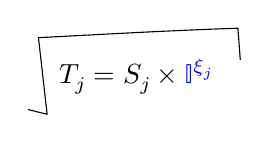
\begin{tikzpicture}[baseline=(lmfixtwentyfour.base),line cap=round,line join=round]
\node[inner sep=2.5pt] (lmfixtwentyfour) {$T_j=S_j\times\unsure{\mathbb I}^{\unsure{\xi_j}}$};
\draw[line width=.4pt]
([xshift=-3mm,yshift=-1mm]lmfixtwentyfour.south west)
-- ([xshift=-.6mm,yshift=-1.6mm]lmfixtwentyfour.south west)
-- ([xshift=-1.7mm,yshift=1.8mm]lmfixtwentyfour.north west)
.. controls ([xshift=6mm,yshift=2.2mm]lmfixtwentyfour.north west) and ([xshift=-7mm,yshift=2.7mm]lmfixtwentyfour.north east) ..
([xshift=2mm,yshift=3mm]lmfixtwentyfour.north east)
-- ([xshift=2.3mm,yshift=-1mm]lmfixtwentyfour.north east);
\end{tikzpicture}} (où $\unsure{\mathbf I|\mathbb I}=[-1,+1]$), $\varepsilon_j=\{j'\in\unsure{J|\mathbf I}\mid j'\text{ sur }i\}$\inserted{$\simeq$ ens. des \uline{orientations} de $S_j$}, $\unsure{\mathbf I^{\varepsilon_j}|\mathbb I^{\varepsilon_j}}$ tordu par $\varepsilon_j$, de sorte qu'on a un homéomorphisme can.

\[
(25)\qquad \partial T_j\simeq\partial\Delta_j.
\]
\inserted{\unsure{i.e.} $\partial T\simeq\partial V_0$ \deleted{\unsure{id}} \unsure{la} \uline{renverse}}

\margin{de sorte que $X_g=\unsure{V_0|U_0}\amalg_{\partial\Delta}T$ (où $\Delta=\coprod_1^g\Delta_j$, $T=\coprod_1^gT_j$) est \uline{\unsure{orienté|orientée}}}

\margin{NB. $T_j$ est canoniquement orienté et l'isom (25) \uuline{respecte} comme \unsure{il se doit|doit} l'\unsure{orientation}}

Ceci posé, l'antipodisme $\tau$ \unsure{induit} sur chaque $\unsure{\partial T_i|\partial T_j}$ \inserted{$\simeq S_j\times\varepsilon_j$}, \deleted{\illegible{1}}\inserted{l'}anti-involution \inserted{canonique} \deleted{\unsure{qui}} \inserted{\unsure{provenant de cette}} \unsure{expression} de $\partial T_i$, qui échange les deux composantes connexes.

Pour \inserted{\unsure{tt|$\forall$}} $j\in\unsure{I|I'}$, on prolonge $\dot\tau|\partial T_j$ à $T_j$ en deux anti-involutions $\dot\tau_j$, \inserted{$\dot\tau'_j$} de $T_j$, \deleted{et on} \deleted{\illegible{1} $T_j$} de telle façon que

\scanpage{453}
\mspage{229}

a) \deleted{pour $j\in I'$}, $\dot\tau_j$ soit sans points fixes

b) \deleted{pour $j\in I'$}, $\dot\tau'_j$ ait un ens. de pts fixes homéomorphe à $S_j$ par la projection $T_j^{\unsure{\dot\tau_j|\dot\tau'_j}}\longrightarrow S_j$ (cf. plus bas \unsure{\}} pour des choix \unsure{particuliers} \unsure{et} explicites \unsure{\}}. --- on \unsure{voit|verra} qu'on peut $\unsure{\overline{\mathrm m}|=}$ supposer $T_j^{\unsure{\dot\tau_j|\dot\tau'_j}}=S_j\times\{0\}$).

Soit, pour tte partie $I'\subset I$, $\tau_{I'}$ l'anti-involution de $X_g=V_0\amalg_{\partial T}T$ (où $V_0=X_0\setminus\bigcup_{j\in J}D'_j$) qui coïncide avec $\tau$ sur $V_0$, avec $\tau'_j$ sur $T_j$ pour $j\in I'$, avec $\unsure{\tau_j^0|\dot\tau_j}$ pour $j\in I\setminus I'$. Alors l'on a
\[
(26)\qquad X_g^{(\tau_{I'})}=\bigcup_{j\in I'}(S_j\times\{0\})
\]
donc si $\operatorname{Card}I'=i$ $(0\leq i\leq g)$, alors $\tau_{I'}$ est une $\sigma_i$.

Choix des $\dot\tau_j$, $\dot\tau'_j$. On choisit un isomorphisme $S_j\simeq\unsure{\mathbb U|\mathbf U}\overset{\unsure{\mathrm{df}}}{=}\{z\in\mathbb C\mid |z|=1\}$, d'où une orientation de $S_j$, et une bijection $\varepsilon_j\simeq\{\pm1\}$, \inserted{d'où $\unsure{\mathbf I^{\varepsilon_j}|\mathbb I^{\varepsilon_j}}\simeq\unsure{I|\mathbf I}=[-1,+1]$} et on prend ;
\[
(27)\qquad
\left\{\begin{aligned}
\dot\tau_{\unsure{j|g}}(z,t)&=\deleted{(\unsure{-z|z},-t)}\;(-z\exp\unsure{\pi it},-t)\\
\dot\tau'_{\unsure{j|g}}(z,t)&=(z\deleted{\unsure{\exp\pi it}},-t)
\end{aligned}\right.
\]

\margin{\uline{NB} Pour la définition \unsure{de|des} $\dot\tau'_j$, on n'a pas besoin du choix d'un iso $S_j\simeq\unsure{\mathbb U|\mathbf U}$ (27)}

\deleted{On a bien $\dot\tau^2$} On a bien $\dot\tau^2=\mathrm{id}$, $\dot\tau'{}^2=\mathrm{id}$
\[
\dot\tau|\partial T=\dot\tau'|\partial T=\tau|\partial T,
\]
D'ailleurs

\scanpage{454}

On note que
\[
(\dot\tau'\dot\tau)^2
=\dot\tau'\dot\tau\dot\tau'\dot\tau
=\bigl((z,t)\longmapsto(z\exp 2i\pi t,t)\bigr)
\]
ce n'est pas l'application identique --- \unsure{l'ens.} de ses pts fixes est égal à : \deleted{\unsure{$S_j$}}
\unsure{l'ens.} des $(z,t)$ tels que $t\in\{-1,0,+1\}$ --- i.e.
\[
T_j^{(\dot\tau'_j\dot\tau_j)^2}
=S_j\times[\partial\unsure{\mathbf I|\mathbb I}^{\varepsilon_j}\cup\{0\}]
\tag{28}
\]

\deleted{\unsure{On a}}

\deleted{Pour \unsure{pouvoir} écrire}

Soit \unsure{$\rho_j=$.}
\[
\dot\rho_j=\dot\tau'_j\dot\tau_j^{\deleted{\illegible{1}}}
\qquad [(z,t)\longmapsto(-z\exp\pi it,t)]
\tag{29}
\]
--- c'est un \unsure{autom.} de $T_j$ qui est l'\uline{identité} sur $\partial T_j$.
\deleted{et} Pour tt partie $I'$ de $I=J/\tau$, soit

(30)\quad $\rho_{I'}$ l'\unsure{autom.} de $X_g$ qui est l'identité sur
$V_0=X_g-\bigcup_{j\in I-I'}T_j$,
et qui est $\rho_j$ sur $T_j$ pour $j\in I'$.

\margin{Posant $\rho_j=\rho_{\{j\}}$, on aura simplement
$\rho_J=\prod_{j\in J}\rho_j$.
Sauf erreur, $\rho_j$ engendre le groupe
$\unsure{S\Gamma^{!+}(T_j)|S\Gamma^{!*}(T_j)}\simeq\mathbb Z$,
\unsure{donc les $\rho_j$ eng. un groupe} $\simeq\mathbb Z^I$.
\inserted{\unsure{(orienté sur}\illegible{1}\unsure{)}}}

\margin{\uline{NB} On a
$\rho_j=\tau^{}_{\deleted{\unsure{\varnothing}}\{j\}}\tau_{\varnothing}$.}

On aura donc
\[
\left\{
\begin{array}{l}
\tau_{I'}\tau_{I''}
=\rho_{I'_0}^{\deleted{\illegible{1}}}\rho_{I''_0}^{-1\,\deleted{\illegible{1}}}
\\[3pt]
\deleted{\unsure{\tau'_{I'}\tau'_{I''}}=\unsure{\rho_{I'_0}\rho_{I''_0}^{-1}}}
\\[3pt]
\deleted{\unsure{(\tau_{I'}\tau_{I''})}\unsure{\illegible{1}}=\rho_{\unsure{I'_0}}\unsure{\illegible{1}}\rho_{\unsure{I''_0}}\unsure{\illegible{1}}}
\end{array}
\right.
\tag{32}
\]
\deleted{\unsure{et le}}
\inserted{où
\deleted{$\unsure{J}=I'\cup I''-\unsure{I'\cap I''}$}
\deleted{$J=I'\cup I''-(I'\cap I'')$}
$I'_0=I'\setminus I'\cap I''$, $I''_0=I''\setminus I'\cap I''$.}

d'autre part on aura évidemment
\[
[\rho_J,\rho_K]=1\qquad\text{pour }J,K\subset I.
\tag{33}
\]

\uline{Remarque.} Au lieu d'un \unsure{isom.} $S_j\simeq\mathbb U$,
supposons donné plutôt sur

\scanpage{455}
\mspage{230}

$S_j$ une structure de torseur sous $\mathbb U^{\varepsilon_j}$
($\mathbb U$ tordu par $\varepsilon_j$, \unsure{grâce|pris} à l'\unsure{autom.} d'ordre 2
$z\longmapsto z^{-1}=\bar z$ de $\mathbb U$) On peut donc définir
\[
\exp:\underset{\underset{\unsure{\mathbf I|\mathbb I}^{\varepsilon_j}}{\cup}}{\mathbb R^{\varepsilon_j}}
\longrightarrow\mathbb U^{\varepsilon_j}
\tag{36}
\]
de façon évidente, d'où des \deleted{applications}
\inserted{\uline{anti-involutions}}
$\dot\tau_j,\dot\tau'_j:T_j\xrightarrow{\sim}T_j$ par les formules (27).

Si p.ex. on choisit des disques $D'_j$ tels que leurs bords soient des \uline{cercles}
\unsure{euclidiens}, alors il y a sur chaque \deleted{\unsure{$S_j$}} $\partial D'_j$
une structure de torseur sous un groupe $\mathbb U^{\varepsilon_j}$,
\unsure{invariant|invariante} par antipodisme, et qui passe donc au quotient.
Dès lors tout \unsure{autom.} de $(X_0,(D'_j))$ qui respecte cette
\deleted{\unsure{montre que le}}
structure supplémentaire de torseurs --- et notamment tt \unsure{autom.} qui respecte
la structure \uline{métrique}, \deleted{\unsure{respecte}} opère sur $X_g$ en commutant
au système des $\tau_j,\tau'_j$ en un sens évident.

\unsure{Égal\textsuperscript{t}}, si on \deleted{prend} \inserted{retient} sur $X$
\unsure{la|les} structure \uline{\unsure{conforme|conformes}} seul\textsuperscript{t}, et si on

\scanpage{456}

choisit dans chaque $D'_j$ un ``centre'' $a'_j$, de façon compatible avec l'involution,
alors le choix des $a'_j\in\mathrm{Int}(D'_j)$ définit une structure de torseur sur
$\partial D'_j$\unsure{\textsuperscript{*}}, et ces structures sont invariantes par les
transformations conformes qui respectent \unsure{l'ens.} des pts $a'_j$.

\margin{\uline{NB} On ne suppose plus \unsure{néc.} que $D_j$ soit un cercle,
\unsure{seulement} que $\partial D_j$ pas trop \deleted{\illegible{1}} \unsure{sauvage}.
Si $\partial D_j$ est un cercle, cette définition coïncide avec la précédente
\unsure{ssi} \unsure{$a_j$|$a'_j$} est le centre \unsure{du|de ce} cercle\ldots}

\uline{Re-NB.} Pour définir $\tau_j$ sur $T_j$, il suffit de \unsure{nettement}
moins de données que d'une structure de torseur topologique sur $T_j$.
Écrivant \inserted{pour $(z,t)\in S_j\times\unsure{\mathbf I|\mathbb I}^{\varepsilon_j}$}
\[
\tau_j(z,t)=(u_t(z),-t)
\tag{37}
\]
où $u_t:S_j\xrightarrow{\sim}S_j$ est un \unsure{homéom.} dépendant continûment de $t$,
écrivant que $\tau_j|\partial T_j=\tau|\partial T_j$, on trouve la condition
\[
\text{a)}\quad u_t=\deleted{\unsure{u_1=}}\mathrm{id}
\quad\text{si }t\in\partial\unsure{\mathbf I|\mathbb I}^{\varepsilon_j}\simeq\varepsilon_j
\]

\margin{\unsure{ça} s'écrit, si $S_j$ est orienté, $u_1=u_{-1}=\unsure{0}$.}

écrivant que $\tau_j^2=\mathrm{id}$ on trouve la condition
\[
\text{b)}\quad u_{-t}=u_t^{-1}
\qquad(t\in\unsure{\mathbf I|\mathbb I}^{\varepsilon_j})
\]
et écrivant que $T_j^{\tau_j}=\varnothing$ on trouve
\[
\text{c)}\quad u_0\text{ sans points fixes}.
\]

Si une orientation est choisie, les $t\longmapsto u_t$ satisfaisant a) b) c)
correspondent aux applications
$[0,1]\xrightarrow{t\mapsto u_t}\deleted{\unsure{\mathrm{Homéom}}}\inserted{\unsure{\mathrm{Aut}}}(\unsure{S_j|S_1})$
telles que $u_1=\mathrm{id}$, $u_0$ ss pt fixe
\deleted{\illegible{2}}\inserted{\uuline{et d'ordre 2}}.
(Le cas \unsure{envisagé} plus haut est celui où
$\unsure{t|*}\longmapsto u_{1-t}$ provient d'une représentation continue
$\mathbb R\longrightarrow\mathrm{Aut}(\unsure{S_j|S_1})$\ldots)

\scanpage{457}
\mspage{231}

\uline{Remarques} On peut se proposer de déterminer la structure de toutes les anti-involutions \inserted{$\tau$} sur un cylindre \inserted{orienté} $T\simeq S\times\unsure{\mathbf I^{\varepsilon}|\mathbb I^{\varepsilon}}$ $(\varepsilon=\operatorname{Or}(S))$ qui \deleted{\unsure{induisent}} n'ont pas de pt fixe sur le bord --- ce qui implique déjà qu'\deleted{elles}\inserted{$\tau$} \unsure{permute|permutent} les deux composantes connexes du bord. Plus généralement, les anti-involutions \inserted{$\tau$} d'une \deleted{\unsure{variété}}\inserted{surface} \uline{à bord} orientée $\unsure{X}$, n'ayant pas de pt fixe sur $\partial\unsure{X}$, correspondent aux variétés à bord $\unsure{Y}$ \unsure{munies} d'une partie à la fois \unsure{ouverte} et \unsure{fermée} $(\partial Y)'$ de $\partial Y$ --- en associant à une telle $\unsure{(Y,(\partial Y)')}$ son \uline{``\unsure{doublement}'' orienté} relativement à $(\partial Y)'$ --- à $X,\sigma$ correspondant $(X/\sigma,\operatorname{Im}X^\sigma\longrightarrow X/\sigma)$. Si $X$ est connexe, \inserted{compact,} $Y$ est \inserted{compacte,} \uline{non orientable}, supposons que \unsure{son type} $(\gamma,j)$, \deleted{soit} et \deleted{\unsure{card} $\pi_0$} \unsure{soit} \inserted{$0\leq i\leq j$, et,} $\unsure{i|i'}=\operatorname{card}(\pi_0((\partial Y)'))$\inserted{$={}\operatorname{card}\pi_0(X^\sigma)$}. Donc $\chi(Y)=1-(\gamma+j)$, et on \unsure{sait|voit} de suite que \deleted{$\chi(X)=\chi_!(\operatorname{Int}(X))$} (car le $\chi$ d'un cercle est nul)
\[
\begin{split}
\chi(X)&=\chi_!\left(\underbrace{X\setminus(\unsure{X\mid\partial Y})}_{\unsure{X\mid\operatorname{Int}(Y)}}\right)\\
&=2\chi_!(\operatorname{Int}Y)=2\chi(Y)=2(1-(\gamma+j))
\end{split}
\]
donc si $X$ est de \deleted{genre}\inserted{type} $(g,\nu)$, on aura \inserted{$\chi(X)=2-2g\unsure{-|+}\nu$}
\[
\deleted{\unsure{g+\nu}}\quad 2-2g\unsure{-|+}\nu=2(1-(\gamma+j))
\]
i.e.
\[
(38)\qquad g+\frac{\nu}{2}=\gamma+j
\]

\margin{pas vrai ! Si $Y$ orientable de type $(\gamma,j)$ (\unsure{même|avec} $0\leq i\leq j$) on aura
\[
(39)\qquad\left\{\begin{array}{l}
g+\dfrac{\nu}{2}=2\gamma+j-1\\
\nu=2(j-i)
\end{array}\right.
\]
i.e. $i=j-\dfrac{\nu}{2}$ (comme dans le cas ci-contre)}

\scanpage{458}

(cela exige que $\nu$ soit pair, ce qui était évident à priori, car $\sigma$ doit permuter les éléments de $\pi_0(\partial X)$ entre eux sans \inserted{y} avoir de pt fixe\ldots)
\deleted{Dans le cas actuel $g=1,\nu=2$ on \unsure{trouve|trouvera} donc}
\deleted{$\gamma+i=2$}
\deleted{d'où les possibilités}
\deleted{$\gamma=2,\ i=0$}
\inserted{Mais j'ai oublié de noter que $\nu$ est déterminé en fonction de $(\gamma,j,i\inserted{={}\unsure{\operatorname{card}((\partial Y)')}})$ par}
\deleted{$\nu=2(j-i)+\unsure{i^{\varepsilon}|i}=2j-i$}
\deleted{$\gamma=2(j-i)$ \unsure{donc}}
\deleted{\unsure{doit avoir}}
\[
(39)\qquad \nu=2(j-i)
\]
i.e. \uline{$i=j-\dfrac{\nu}{2}$}.

Donc il faut ici (pour $g=0,\nu=2$) chercher $(\gamma,j,i)$, avec $\gamma\in\mathbb N,\ 0\leq i\leq j\in\mathbb N$, tels que l'on ait $\nu=2(j-i)$ i.e. $j-i=1$ i.e. $i=j-1$, et $\gamma+j=1$, ce qui donne la \inserted{seule} possibilité (comme $i$ doit être $\geq0$ donc $j\geq1$)

a) $\gamma=0,\ j=1,\ i=0$ \unsure{:|.}

\deleted{b) $\unsure{\gamma=1|\gamma=0},\ \unsure{j=0|j=1},\ i=0$.}

Le cas a) correspond au cas où \deleted{\illegible{1}} $T^\sigma=\varnothing$, \deleted{il \illegible{2} \unsure{nécessairement} une composante connexe, et} se déduit du plan projectif réel en y faisant \deleted{deux}\inserted{un} \unsure{trou|trous}, \inserted{à bord (d'où ruban Möbius)} et en \deleted{bordant l'un d'eux par}\inserted{prenant le \deleted{\unsure{rev. orienté}} doublement orienté}. \deleted{relativement à l'un de ces trous.}

Le cas où $T^\sigma\neq\varnothing$ donnera nécessairement un quotient \inserted{$Y$} \uline{orienté}, on doit avoir pour son type $\unsure{(\gamma,j)}$ (comme $j\geq1$), le seul cas :

\scanpage{459}
\mspage{232}

b) $\gamma=0,\ j=2,\ i=1$ (quotient \uline{orienté})

déduit de la sphère à deux trous i.e. du cylindre, en prenant le doublement orienté \unsure{p.r.} à \uline{un} des trous. \deleted{C'est bien les}

C'est bien les deux cas obtenus \unsure{resp.\textsuperscript{t}} par $\dot\tau$ et $\dot\tau'$ dans les formules (27).

Je voudrais maintenant construire une situation (sous les conditions de la proposition) mettant en évidence un maximum de \unsure{symétries} --- il est vrai que l'on pourrait \unsure{travailler} avec \deleted{\unsure{le} \illegible{1} \unsure{des}} les \unsure{autom.} de $X_0$ \unsure{commutant} à l'antipodisme\inserted{$\tau$}, \inserted{invariant \unsure{l'ens} des $D'_j$,} et respectant (disons) des structures de \unsure{torseurs|torseur} topologiques sur \unsure{l'ens.} des $\partial D'_j$ --- ou ce qui revient \unsure{natl.} au $\overline{\mathrm m}$ (à \unsure{indétermination} de multiplication par $\unsure{\tau|2}$ près) les \unsure{autom.} de $Y_0$ qui \deleted{\illegible{1}} \unsure{invarient|invariant} $D=\bigcup_{i\in I}D_i$, et \unsure{respectent|respectant} des structures de \unsure{torseur|torseurs} sur \deleted{les bords} les comp. conn. $\partial D_i$ de $\partial D$. On prévoit que (travaillant mod isotopie) on \unsure{aura|obtient} un groupe

\margin{non, \uline{sans} indétermination, en relevant \unsure{défini|à la sphère} de façon à \unsure{respecter} \unsure{les orientations|l'orientation}\ldots}

\scanpage{460}

qui sera voisin d'un groupe de tresses, et sans doute calculable sans grand mal --- et en \inserted{\unsure{le}} mettant ens. avec le groupe engendré par les opérateurs précédents, on trouvera peut être un démarrage pour \unsure{engendrer} p.ex. \unsure{$\mathcal T_g$|$\Pi_g$} par générateurs \inserted{(anti-involutifs ?)} et relations.

Considérons le \deleted{\unsure{ss}} groupe $G$ de $A_g=\operatorname{Aut}X_g$ engendré par les \deleted{\illegible{1}}\inserted{$\tau_{I'}$} $(I'\in I)$, \deleted{les} Soit $\mathcal H$ \deleted{commutateurs de générateurs sont dans} le sous-groupe engendré par les $\rho_j$ $(j\in I)$. On a
\[
\begin{aligned}
\tau_{I'}\rho_j\tau_{I'}
&=\deleted{\unsure{(\tau_{I'}(\tau_{\{j\}}\tau_{\varnothing})\tau_{I'})}}
\tau_{I'}(\tau_{\{j\}}\tau_{\varnothing})\tau_{I'}\\
&=(\tau_{I'}\tau_{\{j\}})
\underbrace{(\tau_{\varnothing}\tau_{I'})}_{\deleted{\unsure{\rho_{I'_0}}}\unsure{\rho_{I'}}}
\in\mathcal H
\end{aligned}
\]
par la formule \unsure{(31)|(32)}, donc $\mathcal H$ est un sous-groupe invariant.

Les formules (32) montrent que $G/\mathcal H$ est un groupe \uline{commutatif}, \deleted{\unsure{isomorphe à}}\inserted{et $\overline{\mathrm m}$ qu'il est \unsure{isomorphe à}} $\pm1$ par le caractère d'orientation (tous les $\tau_{I'}$ sont égaux mod $\mathcal H$).
\scanpage{461}
\mspage{233}

Considérons comme élément de référence de $\mathcal H^{-}$ l'élément
\[
(40)\qquad \tau=\tau_{\varnothing}\qquad
\text{(anti-involution ss pts fixes de $X_g$)}
\]
on trouve alors \inserted{par (32)} que pour $I'\subset I$
\[
(41)\qquad \tau_{I'}=\rho_{I'}\tau=
\left(\prod_{j\in I'}\rho_j\right)\cdot\tau\quad
\deleted{\unsure{=\rho_h}}
\]
\margin{on voit de suite, comme $\tau^2=1$, $\tau_{I'}^2=1$, que
$\tau_{I'}=\tau_{I'}^{-1}=\tau\rho_{I'}^{-1}$
\unsure{donc} $\tau\rho_{I'}\tau=\rho_{I'}^{-1}$
\unsure{ce qui est $(42)$|ce qui $\Rightarrow(42)$}}
d'ailleurs on aura, pour \inserted{$\unsure{j|i}\in I$}
\[
\tau\rho_{i}\tau
=\tau_{\varnothing}\left(\tau_{\{\unsure{j|i}\}}\tau_{\{\varnothing\}}\right)
\tau_{\{0\}}
=\tau_{\varnothing}\tau_{\{j\}}=\rho_j^{-1}
\]
\[
(42)\qquad \tau\rho_{i}\tau^{-1}=\rho_{i}^{-1}.
\]

Ainsi $\mathcal G$ apparaît comme le produit semi-direct de $\mathcal H\simeq\mathbb Z^I$, et de
\deleted{\illegible{2}}
$\{\pm1\}\simeq\{1,\tau\}$ y opérant par la symétrie
$\rho\longmapsto\rho^{-1}$. Donc pour \uline{tout} $\rho\in\mathcal H$,
\unsure{\deleted{$\tau\rho$} on a}
$(\tau\rho)^2=1$, i.e. pour tt
$\sigma\in\mathcal H^{-1}$,
$\sigma$ \deleted{\illegible{1}} \uline{est une anti-involution} !
Comme $\sigma$ coïncide avec $\tau$ sur
$V_0=X_g-\bigcup_{\unsure{j|i}\in I}\operatorname{Int}(T_j)$,
on voit que l'ens des pts fixes de $\sigma$ est contenu dans
$\bigcup_{i\in I}\operatorname{Int}(T_i)$, et pour calculer l'indice de $\sigma$,
i.e. $\operatorname{card}\pi_0(X_g^\sigma)$, il suffit de prendre la somme des
\margin{460}

\scanpage{462}

indices dans les $T_j$. Or dans $T_j$, on a \inserted{(29)}
$\rho_j(z,t)=(-z\exp\pi it,t)$, et par récurrence
\[
(43)\qquad \rho_j^{n_j}(z,t)=\left((-1)^{n_j}z\exp n_j\pi it,t\right)
\]
donc
\[
(44)\qquad \tau\rho_j^{n_j}(z,t)=
\left((-1)^{n_j+1}z\exp(n_j+1)\pi it,-t\right)
\]
et \deleted{\illegible{1}} $(z,t)$\inserted{$\in T_j$} est pt fixe de
$\unsure{z|\tau}\rho_j^{n_j}$ \unsure{ssi|ss}
$t=0$, \deleted{\unsure{si|et}} et $n_j$ est \uline{impair}, donc
\[
(45)\qquad T_j^{\tau\rho_j^{n_j}}=
\begin{cases}
\varnothing&\text{si $n_j$ pair}\\
S_j\times\{0\}&\text{si $n_j$ impair}
\end{cases}
\]

donc
\[
\begin{gathered}
(46)\qquad \text{Indice de }u=\tau\prod_j\rho_j^{n_j}\text{ est égal au cardinal}\\
\text{de l'ens. }I'_u\text{ des }j\in I\text{ tels que }n_j\\
\text{\unsure{soit|sont} impair}
\end{gathered}
\]

Il en résulte \inserted{par des raisons générales} que $u$ est conjugué dans
$\mathcal A_g=\operatorname{Aut}(X_g)$
\inserted{(par un élément de $\unsure{A_g^+|\widetilde A_g^+}$)}
à $\tau_{I'}=\rho_{I'}\tau=\tau\rho_{I'}^{-1}$ \unsure{ou aussi}
$\rho_{I'}^{-1}\tau=\tau\rho_{I'}$ ---
\deleted{
\unsure{mais} \illegible{4}
\inserted{on a l'égalité \illegible{2} $\mathcal H$}
\unsure{dans le groupe} $\mathcal G$ (\unsure{trop petit}).
\illegible{4} $\rho\in\mathcal H$, \illegible{2}
\unsure{les questions}, d'une part
\[
\unsure{(\tau\rho)^{-1}}\cdot\rho_{I'}(\tau\rho)
=\unsure{\tau\rho\rho_{I'}}
\]
en introduisant des groupes de symétries supplémentaires, d'autre part en
\deleted{\unsure{l'agrandissant}, en} \unsure{complétant}
chaque $T_j$ par une \unsure{configuration} plus
}
\margin{\deleted{
\[
\unsure{(\tau\rho)(\tau\rho')(\tau\rho)^{-1}}
=\underset{\text{\deleted{\illegible{1}}}}{\tau\rho}\,
\underbrace{\tau\rho'\rho^{-1}\tau}_{\rho\rho'^{-1}}
=\tau\rho^{2}\rho'^{-1}=\tau\rho''
\]
dès que $\rho^2=\rho'\rho''$, \unsure{c.à.d.|càd.}
\illegible{3} $\tau\rho'$ est \unsure{conjugué} \illegible{1}
$\unsure{\tau\rho''}$ dans $\mathcal G$, dès que
$\rho'\rho''\in\mathcal H^2$
}}
\margin{461}

\scanpage{463}
\mspage{234}

Mais si $\tau\rho',\tau\rho''\in\mathcal G^-$, $(\rho',\rho''\in\mathcal H)$, et si
$\rho\in\mathcal H$, la relation
\[
\rho(\tau\rho')\rho^{-1}=\tau\rho''
\]
équivaut à
\[
\underbrace{\tau\rho\tau}_{\rho^{-1}}\rho'\rho^{-1}=\rho''
\qquad\text{i.e.}\qquad \rho^2=\rho'\rho''^{-1}
\]
donc $\tau\rho'$ et $\tau\rho''$ sont conjugués par un élément de $\mathcal H$
\unsure{ssi|ss} $\rho'\rho''^{-1}\in\mathcal H^2$ -- ce qui précise l'observation précédente\ldots

La façon la plus riche en symétries simples pour disposer les $2g$ trous antipodiques
$D_j$ me semble la suivante. On \deleted{\illegible{1}} considère
la sphère euclidienne, avec \unsure{l'}action du groupe dihédral
$\unsure{\mathbb D_{2g}|\mathbf D_{2g}}$ -- par exemple, quand c'est la sphère de Riemann qui est
considérée comme riemannienne, par le choix de l'antipodisme comme étant
\[
(47)\qquad \tau z=-\frac{1}{\overline z}
\]
on prend l'action type du groupe dihédral (avec comme pôles les points $0,\infty$, et
comme équateur le cercle unité $\mathbb U=\{z\in\mathbb C\mathbin{:}|z|=1\}$),
\deleted{par} en écrivant
$\unsure{\mathbb D_n|\mathbf D_n}$ comme $\subset\operatorname O(\deleted{\unsure{3}}2,\mathbb R)$,
comme un produit $\frac12$ direct de
\deleted{\unsure{$\mathbb Z/2\mathbb Z$}}\inserted{$\{\pm1\}$} par $\mu_n(\mathbb C)=\mu_n$,
le couple $(\zeta,\alpha)$ $(\zeta\in\mu_n,\alpha\in\deleted{\unsure{\mathbb Z/2\mathbb Z}}\inserted{\{\pm1\}})$ opérant par
\[
(48)\qquad u_{\zeta,\alpha}(z)=\zeta z^\alpha
\]
\margin{462}

\scanpage{464}

On peut d'ailleurs l'élargir en un groupe
$\mathbb D_n^\sim=\mathbb D_n\times\mathbb Z_{/2}$,
où le deuxième facteur $\mathbb Z_{/2}$ est engendré par l'antipodisme (47)
(qui commute à $\mathbb D_n$ --- de $\overline{\mathrm m}$ d'ailleurs
que l'anti-involution $z\longmapsto\frac{1}{\bar z}$, qui a comme
ens des pts fixes $\mathbb U$ et n'est autre que la symétrie p.r. à
l'équateur, leur composé $z\longmapsto-z$ étant la symétrie p.r. à
l'axe des pôles \ldots) donc de regarder les transformations
\[
u_{\zeta,\alpha,\beta}\deleted{(z)}=\unsure{\zeta}u_{\zeta,\alpha}\tau^\beta
\qquad
(\zeta\in\mu_n,\ \alpha\in\{\pm1\},\ \beta\in\mathbb Z_{/2})
\]
donc
\[
u_{\zeta,\alpha,\beta}z=
\begin{cases}
u_{\zeta,\alpha}(z)=\zeta z^\alpha&\mathrm{si}\ \beta=0\\
u_{\zeta,\alpha}(-\frac{1}{\bar z})=-\zeta\bar z^{-\alpha}
&\mathrm{si}\ \beta=1
\end{cases},
\]
mais on se \unsure{rappellera} que $\tau$ renverse l'orientation,
donc \deleted{\illegible{1}}\inserted{est à}
\deleted{\unsure{plus}}\inserted{manier} avec
réserve pour ce qui concerne le "transport de structure" dans
la situation présente.

Ici $n=2g$, $\mathbb D_{\unsure{2g|n}}$ est d'ordre $4g$, et
$\mathbb D_n^\sim$ d'ordre $8g$. On prend sur l'équateur une
trajectoire $\unsure{\mathcal J|\mathbb J}$, de $\mu_n=\mu_{2g}$, p.ex.
\unsure{les|ici} \unsure{justement}
\deleted{\unsure{les}} ($\mu_{2g}$
\inserted{\unsure{l'ens} des racines \unsure{$2g$ ièmes} de l'unité}
lui-$\overline{\mathrm m}$, \unsure{vu}\deleted{\illegible{1}}
\unsure{pour} sous-ens. de la sphère) comme l'ens des "centres"
des disques $D'_i$. On choisit un disque $D'_0$ autour du
\unsure{point|pt} $P_0$ (assez petit pour ce qui va suivre), et on
prend les \unsure{transformés|transformées} de $D'_0$ par les
$\zeta\in\mu_n$.

\margin{il faut \unsure{simplemt} que $D'_0$ ne
\unsure{rencontre} pas $\unsure{\zeta_0|\zeta}D'_0$,
\unsure{où} $\zeta=\exp\frac{2i\pi}{2g}$}

\margin{463}

\scanpage{465}
\mspage{235}

Ces choix étant faits, la surface $X_g$ est déterminée sans
\unsure{ambiguité|ambiguïté}, et le groupe $\mathbb D_{2g}$ y opère par transport de
structure, en permutant entre eux les $g$ cylindres $T_i$,
\unsure{correspond.ts|correspondants} aux éléments de
\inserted{$\unsure{\mathcal J|\mathbb J}/\tau=$}$\unsure{\mathcal J|\mathbb J}/\{\pm1\}$ i.e.
aux paires d'éléments antipodiques de $\unsure{S|\mathcal J}$,
i.e. aux "diagonales" du polygone à $2\mu$ côtés
qu'ils \deleted{\unsure{forment}}\inserted{déterminent}
sur l'équateur. Le groupe $\mathbb D_{2g}$ normalise
\deleted{\illegible{1}} le groupe $\mathcal G$, de façon précise
on aura, pour $u\in\mathbb D_{2g}$
\[
\tag{49}
u\tau_{I'}u^{-1}=\tau_{u(I')}
\]
pour $I'\subset I=\unsure{\mathcal J|\mathbb J}/\tau$, en tenant compte de
l'opération de $\mathbb D_{2g}$ sur $I$. On aura donc en
particulier, désignant par $\tau_g$\inserted{$=\tau_\varnothing$}
l'extension \margin{\deleted{(50)}} de l'antipodisme de la sphère $X_0$
(ou plutôt de $\unsure{\tau}\vert V_0$) en un antipodisme
sans pts fixes de $X_g$, noté $\tau$ précédemment:
\[
\tag{50}
u\tau_g u^{-1}=\tau_g
\qquad\text{i.e. $\tau_g$ commute à l'action de $\mathbb D_n$}
\]
\[
\deleted{\unsure{(51)}}\qquad
u\rho_j u^{-1}=\rho_{u\unsure{(}j)}
\]

On peut donc dire que $\mathbb D_{2g}$ opère sur $\mathcal G$,
d'où un produit $\frac12$-direct $\mathbb D_{2g}.\mathcal G$,
qui opère donc sur $X_g$.
Quant à la question de prolonger de $\overline{\mathrm m}$
l'action \inserted{sur $X_0$,} de $\mathbb D_{2g}^\sim$
\deleted{sur $X_0$} \unsure{tout entier} en une action sur $X_g$,

\margin{464}

\scanpage{466}

ça a été fait sans crier gare, à $\tau_{X_0}$ correspondant
naturellement $\tau_{X_g}=\tau_g$, qui a en effet le bon goût
de commuter à l'action de $\mathbb D_{2g}$.
[Il pourrait sembler plus naturel, il est vrai, dans un
esprit de "transport de structure (\unsure{envers} et contre
tout?)", de faire correspondre à $\tau_{X_0}$ l'opération
$\tau_I$\inserted{\unsure{donné|donnée} par (27)}, qui sur
chaque $T_j$ serait égal à $\tau'_j$
(et sur $V_0$, bien sûr, coïncide avec $\tau_{X_0}$),
$\tau'_j(z,t)=(z,-t)$,
\deleted{donc} l'ens des pts fixes de $\tau_I^{\unsure{2}}$
étant formé des $g$ cercles \unsure{médians} $S_j\times\{0\}$
des $g$ tubes $T_j$. On aura par (41)
$\tau_I=\rho_I\tau_g$, donc $\tau_I$ commute
\unsure{également} à $\mathbb D_n$, puisque $\tau$ et
$\rho_I=\prod_{i\in I}\rho_i$ y commutent.
Mais il \unsure{ne|me} semble pas \unsure{important} pour le moment
quelle convention nous \unsure{adoptons}]

On peut donc dire aussi que le groupe $\mathbb D_{2g}^\sim$
opère sur $\mathcal H$ --- cette opération prolongeant celle
de $\tau_g$\deleted{\unsure{par}}, identifié maintenant à un
élément de $\mathbb D_{2g}^\sim$, i.e. à l'antipodisme dans
$\mathbb D_{2g}^\sim$ --- et le produit $\frac12$ direct
\[
\tag{51}
\mathbb D_{2g}^\sim.\mathcal H\supset\mathcal G
=\deleted{\unsure{\mathcal H}}\{1,\tau_g\}.\mathcal H
\]

\margin{465}

\scanpage{467}
\mspage{236}

opère sur $X_g$.

Il faudrait maintenant, dans cette voie :

1) Expliciter l'action extérieure de ce produit $\frac12$ direct sur le groupe fondamental $\pi_g$, \unsure{avec} une attention toute particulière à l'action du groupe $(\mathbb Z/2\mathbb Z)^3\subset\mathbb D_{2g}^{\sim}$ qui stabilise un des cylindres $T_j$ --- qui dans l'espace euclidien de dim 3 s'interprète comme le groupe des \unsure{chgts} de signe relatif \unsure{au|un} syst. d'axes orthonormé correspondant.

2) Étendre l'action \inserted{sur $\pi_g$} du groupe de Teichmüller (plus ou moins) ``spécial'' de chacun des $T_j$, en l'action d'un groupe analogue d'un ensemble plus grand obtenu en lui rajoutant une ``lanière'' \inserted{$L$} (d'où un tore à 1 trou, et son groupe de Teichmüller spécial, qui \unsure{s'introduisent} de façon naturelle$^*$) \unsure{voire|voir} l'ensemble encore plus grand obtenu en mettant également la lanière antipodique $L'$ (cet ensemble se présente comme un cylindre $(L\cup L')$, ou ``buse'', où on aurait mis un tube $(T_j)$ en travers, et a la structure topologique d'un tore à deux trous.

\figure{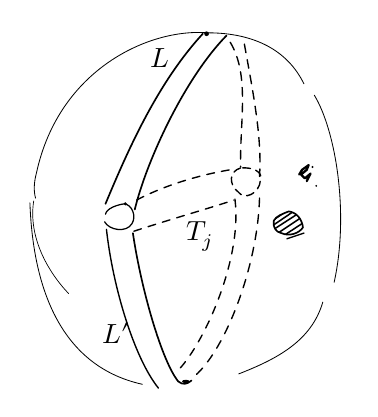
\begin{tikzpicture}[x=.12mm,y=-.12mm,line cap=round,line join=round]
\draw[line width=.3pt] (194,39) .. controls (133,34) and (37,77) .. (13,187) .. controls (10,198) and (10,207) .. (12,214);
\draw[line width=.3pt] (194,39) .. controls (244,39) and (279,58) .. (296,93);
\draw[line width=.3pt] (307,105) .. controls (330,143) and (344,231) .. (328,303);
\draw[line width=.3pt] (316,324) .. controls (304,365) and (268,384) .. (227,400);
\draw[line width=.3pt] (6,219) .. controls (9,303) and (35,391) .. (125,411);
\draw[line width=.25pt] (10,217) .. controls (4,255) and (25,292) .. (47,315);
\draw[line width=.6pt] (189,40) .. controls (142,91) and (111,160) .. (86,220);
\draw[line width=.6pt] (214,42) .. controls (169,88) and (129,176) .. (117,226);
\draw[line width=.5pt] (87,247) .. controls (94,310) and (117,384) .. (142,415);
\draw[line width=.6pt] (115,251) .. controls (124,312) and (146,387) .. (163,408) .. controls (168,412) and (172,411) .. (177,407);
\draw[line width=.45pt] (86,231) .. controls (87,225) and (98,221) .. (106,220) .. controls (114,221) and (119,233) .. (114,241) .. controls (108,251) and (90,248) .. (85,239);
\draw[line width=.5pt,dash pattern=on 1.1mm off .9mm] (218,49) .. controls (239,84) and (228,133) .. (229,181);
\draw[line width=.5pt,dash pattern=on 1.1mm off .9mm] (233,51) .. controls (241,96) and (252,149) .. (249,191);
\draw[line width=.5pt,dash pattern=on 1mm off .7mm] (229,182) .. controls (216,186) and (217,200) .. (226,207) .. controls (233,217) and (249,209) .. (250,195) .. controls (253,186) and (242,181) .. (229,182);
\draw[line width=.5pt,dash pattern=on 1mm off 1mm] (223,215) .. controls (231,278) and (191,366) .. (164,395);
\draw[line width=.5pt,dash pattern=on 1.1mm off 1mm] (249,214) .. controls (247,288) and (211,380) .. (177,405);
\draw[line width=.5pt,dash pattern=on 1mm off .9mm] (119,216) .. controls (155,197) and (197,187) .. (224,183);
\draw[line width=.5pt,dash pattern=on 1mm off .9mm] (116,249) .. controls (156,236) and (198,224) .. (222,216);
\fill (193,40) circle[radius=.3mm];
\fill (171,408) ellipse[x radius=.48mm,y radius=.216mm];
\fill (107,220) circle[radius=.216mm];
\node[inner sep=0pt] at (144,66) {$L$};
\node[inner sep=0pt] at (98,357) {$L'$};
\node[inner sep=0pt] at (186,255) {$T_j$};
\draw[line width=.8pt] (291,189) -- (294,184) -- (301,179) -- (299,184) -- (293,189) -- (297,193) -- (303,188) -- (299,196);
\fill (305,181) circle[radius=.144mm];
\fill (309,201) circle[radius=.132mm];
\draw[line width=.6pt] (264,238) .. controls (266,233) and (275,230) .. (280,228) .. controls (288,229) and (294,236) .. (295,245) .. controls (291,251) and (281,255) .. (272,251) .. controls (266,250) and (263,244) .. (264,238);
\begin{scope}
\clip (264,238) .. controls (266,233) and (275,230) .. (280,228) .. controls (288,229) and (294,236) .. (295,245) .. controls (291,251) and (281,255) .. (272,251) .. controls (266,250) and (263,244) .. (264,238);
\draw[line width=.55pt] (258,241)--(283,224) (260,245)--(288,226) (261,249)--(292,229) (264,254)--(297,232) (271,256)--(300,237) (280,257)--(302,242);
\end{scope}
\draw[line width=.5pt] (278,257) -- (296,251);
\end{tikzpicture}}

\margin{$^*$ C'est essentiellement un $\mathrm{SL}(2,\mathbb Z)$ --- plutôt une extension centrale \unsure{remarquable} de $\mathrm{SL}(2,\mathbb Z)$ par $\mathbb Z$, qui \unsure{rappelle} celle de $\mathrm{SL}(2,\mathbb R)$ par $\mathbb Z$\ldots\ (rev. universel de $\mathrm{SL}(2,\mathbb R)$)}

\figure{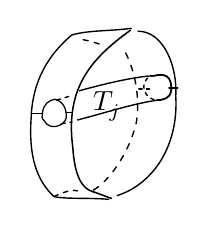
\begin{tikzpicture}[x=.12mm,y=-.12mm,line cap=round,line join=round]
\draw[line width=.5pt] (118,15) .. controls (94,18) and (72,17) .. (55,22) .. controls (24,48) and (13,79) .. (12,109) .. controls (9,151) and (18,176) .. (36,193) .. controls (49,196) and (75,194) .. (94,196);
\draw[line width=.5pt] (125,18) .. controls (153,18) and (167,57) .. (165,87) .. controls (168,137) and (143,179) .. (103,192);
\draw[line width=.55pt] (117,17) .. controls (74,48) and (48,79) .. (56,141) .. controls (58,170) and (65,185) .. (78,188) -- (97,195);
\draw[line width=.5pt,dash pattern=on .65mm off .8mm] (67,27) .. controls (74,28) and (82,31) .. (89,33);
\draw[line width=.5pt,dash pattern=on .75mm off .95mm] (112,41) .. controls (124,65) and (127,94) .. (123,116) .. controls (115,148) and (94,177) .. (78,186);
\draw[line width=.45pt] (24,104) .. controls (25,95) and (31,91) .. (37,90) .. controls (46,92) and (50,101) .. (49,110) .. controls (47,118) and (32,124) .. (26,113) .. controls (23,111) and (23,107) .. (24,104);
\draw[line width=.5pt] (12,105) -- (24,105) (49,104) -- (55,104);
\draw[line width=.5pt,dash pattern=on .5mm off .6mm] (39,91) -- (55,86) (44,116) -- (55,114);
\draw[line width=.5pt] (63,81) .. controls (85,75) and (120,66) .. (143,65);
\draw[line width=.5pt] (61,112) .. controls (88,105) and (122,94) .. (146,91);
\draw[line width=.65pt] (143,65) .. controls (159,61) and (161,72) .. (160,82) .. controls (159,88) and (153,91) .. (145,91);
\draw[line width=.5pt,dash pattern=on .45mm off .55mm] (143,65) .. controls (128,65) and (126,87) .. (144,91);
\draw[line width=.55pt,dash pattern=on .4mm off .55mm] (126,79)--(141,79);
\draw[line width=.7pt] (158,78)--(167,78);
\draw[line width=.5pt,dash pattern=on .6mm off .7mm] (36,193) .. controls (47,188) and (56,185) .. (61,187);
\fill (78,188) circle[radius=.18mm];
\node[inner sep=0pt] at (92,98) {$T_j$};
\end{tikzpicture}}

\margin{466}

\scanpage{468}

Il est possible qu'il faudra considérer de près ce dernier, pour étudier les relations entre \inserted{les} éléments de $\mathcal T_g$ provenant des ensembles précédents\ldots\ Un travail amusant sera de se débrouiller pour écrire les générateurs du groupe $\pi_g$, et surtout la fameuse relation, dans une disposition géométrique relative des ``anses'', qui est une disposition ``\unsure{panachée}'' --- et non plus \uline{sagement} à la queue-leu-leu !

\deleted{Je vois \unsure{apparaître}}

En attendant d'entrer ainsi dans le vif de la structure du groupe de Teichmüller, je vais déjà essayer de décrire des générateurs et relations pour le sous-groupe intéressant qu'on vient d'écrire, $\mathbb D_{2g}^{\sim}\cdot H$.
Je vais prendre les sempiternels générateurs $\varepsilon_0,\varepsilon_1$ de $\mathbb D_{2g}$
\[
\varepsilon_0^2=\varepsilon_1^2=1,\qquad (\varepsilon_0\varepsilon_1)^{2g}=1
\]
et y joindre $\tau=\tau_g$, et \deleted{\illegible{1}} $\rho_0\tau=\tau'$
($\rho_0=\rho_{j_0}$, $j_0$ pt marqué de $I=J/\tau$)
satisfaisant
\[
\tau^2=\tau'^2=1,\qquad
\deleted{[\tau,\varepsilon_0]=\unsure{[\varepsilon_1,\tau]|[\tau,\varepsilon_1]}=}
\]
\[
(\tau\varepsilon_0)^2=(\tau\varepsilon_1)^2=1\quad
\deleted{\unsure{(\tau'\varepsilon_0)^2=(\tau'\varepsilon_1)^2}=1}
\]
\[
(\varepsilon_1\tau')^2=1
\qquad \varepsilon_1\ \text{commute à}\ \tau'
\]

\margin{\uline{NB} $\varepsilon_0$ bouge \unsure{le sommet} du repère, $\varepsilon_1$ l'arête et pas le sommet, donc $\varepsilon_1(j_0)=j_0$}

\margin{\unsure{expriment} la commutation de $\tau$ \deleted{\illegible{1}} à $\varepsilon_0,\varepsilon_1$}

\margin{467}

\scanpage{469}
\mspage{237}

\[
((\varepsilon_0\varepsilon_1)^g\tau')^2=1
\]
\margin{(l'involution $(\varepsilon_0\varepsilon_1)^g$ commute à $\tau'$)}

sauf erreur, ça fait un ensemble de générateurs et relations pour $\mathbb D_{2g}^{\sim}\cdot\mathcal H$ --- en résumé $\varepsilon_0,\varepsilon_1,\tau,\tau'$
\[
\text{(52)}\quad
\left\{
\begin{array}{l}
\varepsilon_0^2=\varepsilon_1^2=\tau^2=\tau'^2=1\\
(\tau\varepsilon_0)^2=(\tau\varepsilon_1)^2=(\tau'\varepsilon_1)^2=1\\
(\varepsilon_0\varepsilon_1)^{2g}=1\\
(\tau'(\varepsilon_0\varepsilon_1)^g)^2=1
\end{array}
\right.
\]

C'est peut-être pas très astucieux comme choix de générateurs, en ce sens que $\varepsilon_0,\varepsilon_1$, ne sont pas du tt sur le même pied que $\tau,\tau'$ --- ce ne sont pas des \uline{anti}-\unsure{involutions}. Il vaudrait mieux prendre $\varepsilon'_0=\tau\varepsilon_0$, $\varepsilon'_1=\tau\unsure{\varepsilon_1}$ de façon à obtenir
\[
\text{(52bis)}\quad
\left\{
\begin{array}{l}
\varepsilon_0^{\prime 2}=\varepsilon_1^{\prime 2}=\tau^2=\tau'^2=1\\
(\tau\varepsilon'_0)^2=(\tau\varepsilon'_1)^2=(\tau'(\tau\varepsilon'_1))^2=1\\
(\varepsilon'_0\varepsilon'_1)^{2g}=1\\
(\tau'(\varepsilon'_0\varepsilon'_1)^g)^2=1
\end{array}
\right.
\]
ce sont essentiellement ``les mêmes'' relations sauf la dernière de la deuxième ligne.

Peut être ce petit jeu avec le tout petit groupe $\mathbb D_n^{\sim}$ opérant sur $\mathcal H$ est un peu une \unsure{amusette} --- le groupe $\mathcal H\simeq\mathbb Z^g$ dans $\mathcal T_g$ suggère beaucoup la situation

\margin{468}

\scanpage{470}

d'un tore maximal dans un groupe $\frac12$ simple, on a vraiment envie d'en \unsure{avoir|voir} une caractérisation intrinsèque dans $\mathcal T_g$ --- ou dans $\unsure{\mathcal S_g|\mathcal G_g|\mathcal C_g}$, ce qui est possible puisque \deleted{\illegible{1}} en tant que groupe de transformations topologiques \unsure{effectives|effectif}, il laisse fixe les points de $V_0\subset X_g$ --- p.ex. les deux pôles, qu'on peut prendre comme pts \unsure{bases|base} pour construire rev. universels et groupes \unsure{fondamental|fondamentale}. Ce sont peut-être les sous-groupes \unsure{abéliens|abélien}-libres maximaux.

On aimerait étudier le normalisateur --- est-ce exactement ce qui provient des autom de $X_g-\bigcup\mathring{T}_i\simeq V_0$ ?

les $\mathrm{SL}(2,\mathbb Z_{\unsure{j}})$ associés aux ``lanières'' à travers le tube \inserted{$T_j$} jouent-ils un rôle analogue à celui des groupes $\mathrm{SL}(2,K)$ ou $\unsure{\mathrm{GP}(1,k)|\mathrm{GL}(1,k)}$ ``de rang 1'' dans la théorie des groupes algébriques réductifs ? Si Jean \unsure{ne|me} ``\unsure{mord}''

\margin{469}
\scanpage{471}
\mspage{238}

pas à la situation, la soumettre peut-être à Carlos, qui est à l'aise tant avec les groupes discrets et leurs générateurs et relations, qu'avec la théorie des $\frac{1}{2}$ simples -- et la topologie ....

\scanpage{472}
\mspage{239}

\uline{33} Étude des revêtements finis -- relation entre les $\mathcal N_{g,\nu},\Gamma_{g,\nu}$ pour $g$ variable.

Soient $(\pi\deleted{,\unsure{a}})$ groupe ext. à lacets profini arithmétisé de type $(g,\nu)$, $\pi'$ un \unsure{ss-grpe|ss-grp} ouvert de $\pi$, d'où une application injective
\[
\mathrm{Discr\acute{e}t}(\pi)\hookrightarrow
\mathrm{Discr\acute{e}t}(\pi'),
\]
on voudrait prouver qu'elle est compatible avec la relation d'équivalence \deleted{\unsure{des}\ \illegible{1}}\inserted{\unsure{de l'arithmétisation|de l'arithmétisabilité}}, de \deleted{\unsure{prouver}} sorte que tte arithmétisation de $\pi$ en donne une de $\pi'$, et de $\overline{\mathrm m}$ pour les \deleted{\unsure{discre}} prédiscrétifications.

On voudrait établir en $\overline{\mathrm m}$ temps que les applications
\[
\begin{array}{lll}
 &P^+(\pi)\longrightarrow P^+(\pi')&\begin{gathered}\text{sur les prédiscrétifications}\\\text{orientées}\end{gathered}\\[1em]
\text{et}&A(\pi)\unsure{\longrightarrow|-}A(\pi')&\text{sur les arithmétisations}
\end{array}
\]
sont injectives. Pour prouver ces points, on est ramené au cas où $\pi'$ est invariant caractéristique. (Cf \S\,28, diagramme 7, \unsure{ff}) Choisissant

\scanpage{473}

une discrétification $\pi_0$ de $\pi$, donc $\pi'_0$ de $\pi'$, on trouve alors
\[
\unsure{\widehat{\widehat{\mathcal G}}}(\pi_0)\longrightarrow
\unsure{\widehat{\widehat{\mathcal G}}}(\pi'_0)
\]
et on a

\textcircled{1} L'hom $\unsure{\widehat{\widehat{\mathcal G}}}(\pi_0)\unsure{\longrightarrow}\unsure{\widehat{\widehat{\mathcal G}}}(\pi'_0)$ envoie $\mathcal M(\pi_0)$ dans $\mathcal M(\pi'_0)$

on aura donc un diagramme (\unsure{variante|parent} de celui du \S\,28)
\diagram{\begin{tikzcd}[ampersand replacement=\&,column sep=large,row sep=large]
\unsure{(1)} \&
\widehat{\mathcal G}^{+}(\pi_0)
 \arrow[r,hook,no head] \arrow[d,hook] \&
\mathcal M(\pi_0) \arrow[r,hook,no head] \arrow[d,hook] \&
\widehat{\widehat{\mathcal G}}(\pi_0) \arrow[d,hook] \\
\& \widehat{\mathcal G}^{+}(\pi'_0)
 \arrow[r,hook,no head] \&
\mathcal M^{\unsure{\ast|\sharp}}(\pi'_0) \arrow[r,hook,no head] \&
\unsure{\widehat{\widehat{\mathcal G}}}(\pi'_0)
\end{tikzcd}}
qui \deleted{signifie} implique qu'une discrétification $\pi_1$ sur $\pi$ qui donne $\overline{\mathrm m}$ prédiscrétification orientée que $\pi_0$ (resp. $\overline{\mathrm m}$ arithmétisation) définit une \inserted{\unsure{discrét}} $\pi'_1$ de $\pi'$ qui donne $\overline{\mathrm m}$ prédiscr. or. (resp. $\overline{\mathrm m}$ arithm.) que $\pi'_0$. Donc on a bien $\unsure{P}^{+}(\pi)\longrightarrow P^+(\pi')$, $A(\pi)\longrightarrow A(\pi')$, il faut encore exprimer l'injectivité, qui revient aux relations
\[
\begin{gathered}
(2)\quad
\unsure{\widehat{\mathcal G}^{+}}(\pi_0)
=
\unsure{\widehat{\mathcal G}^{+}}(\pi'_0)\cap
\unsure{\widehat{\widehat{\mathcal G}}}(\pi_0),\qquad
\mathcal M(\pi_0)=\mathcal M(\pi'_0)\cap
\unsure{\widehat{\widehat{\mathcal G}}}(\pi_0)
\end{gathered}
\]
\scanpage{474}
\mspage{240}

i.e. un \unsure{autom.} à lacets de $\pi^{+}$ qui, sur $\pi'$, appartient à $\unsure{\widehat{\mathcal G}}(\pi'_0)$ \deleted{\illegible{2}} resp. à $\mathcal M(\pi'_0)$, est déjà dans $\unsure{\widehat{\mathcal G}}(\pi_0)$ resp. dans $\mathcal M(\pi_0)$.

L'assertion \deleted{\illegible{1}} repérée étant admise, l'assertion \inserted{non} repérée signifie aussi que l'hom. can.
\[
(3)\qquad
\mathbb{\Gamma}_a=\mathcal M_a(\pi)/\unsure{\widehat{\mathcal G}}^{+}_a(\pi)
\longrightarrow
\mathbb{\Gamma}_{a'}=\mathcal M_{a'}(\pi')/\unsure{\widehat{\mathcal G}}^{+}_{a'}(\pi')
\]
est \uline{injectif}. Par construction (via $\mathbb{\Gamma}_{\unsure{\mathbb Q}}$) c'est aussi surjectif, donc on trouverait :

\textcircled{2} l'hom. canonique (3) est bijectif

et on trouverait aussi une bijection
\[
(4)\qquad P_a(\pi)\longrightarrow P_{a'}(\pi')
\]
entre \unsure{arithm.} de $\pi$ de type $a$, et arithm. de $\pi'$ de type $a'$, \uline{compatible} avec l'iso. \unsure{(3)}.

Enfin, un résultat dans le cas $\pi'$ \unsure{inv.} car. s'étendrait aussitôt au cas d'une $\pi'\subset\pi$ ouvert quelconque.

Procédant \inserted{p.ex.} comme dans le \S 28 à coups de ``correspondances'' \inserted{arithm. extérieures\unsure{,}} entre

\scanpage{475}

``courbes potentielles'', on trouve un groupoïde connexe (ponctué par les $\widehat{\pi}_{g,\nu}$, p.ex, \deleted{\unsure{)}} qui y sont \unsure{can.} isomorphes), dont le $\pi_1$ ext. est la valeur commune des $\mathbb{\Gamma}_{g*}=\mathbb{\Gamma}_{g,\nu}$.

Pour trouver \unsure{un} l'isom. \inserted{\unsure{canonique}} entre $\mathbb{\Gamma}_{g,\nu}$ et $\mathbb{\Gamma}_{g',\nu'}$, on choisit une \deleted{\unsure{multiple commun}} \inserted{correspondance entre} un $\pi_{g,\nu}$ et $\pi_{g',\nu'}$, p.ex. en \unsure{regardant} \deleted{\unsure{$N$ de $2g-2+\nu$ et $2g'-2+\nu'$}} l'un et l'autre (quitte à passer : de $g,\nu$ à $g,\widetilde{\nu}$ avec $\widetilde{\nu}\geq\nu$, et de $\overline{\mathrm m}$ pour $g',\nu'$ à $(g',\widetilde{\nu}')$ avec $\widetilde{\nu}'\geq\nu'$) comme des sous-groupes finis du $\overline{\mathrm m}$ $\pi_{0,3}$ \unsure{et} d'où
\[
\mathbb{\Gamma}_{0,3}\xrightarrow{\sim}\Gamma_{g,\widetilde{\nu}},
\qquad
\Gamma_{0,3}\xrightarrow{\sim}\Gamma_{g',\widetilde{\nu}'}.
\]

On aimerait maintenant voir ce qui, dans le yoga précédent, est indépendant de toute conjecture. Par exemple, le fait que les \unsure{hom} surjectifs \inserted{\unsure{can.}} $\mathbb{\Gamma}_{g,\nu}\unsure{\longrightarrow}\mathbb{\Gamma}_{g,\nu'}$ ($g$ le $\overline{\mathrm m}$, $\nu'$ constant) n'est pas établi.

Cependant, si on savait que dans la situation du $(\pi,\pi')$ avec $\pi'$ \unsure{inv.} car. on ait
\[
\widehat{\widehat{\mathcal T}}(\pi'_0)\cap
\unsure{\widehat{\mathcal G}}^{+}(\pi_0)
=
\unsure{\widehat{\mathcal G}}^{+}(\pi_0)
\]

\scanpage{476}
\mspage{241}

(qui est un énoncé de nature relativement anodin sur des groupes à lacets profinis) on conclurait à la \uline{bijectivité} de $\mathbb{\Gamma}_{\pi_0}\longrightarrow\mathbb{\Gamma}_{\pi'_0}$ dans cette situation, et on en conclurait que le noyau de $\mathbb{\Gamma}_{\unsure{\mathbb Q}}\longrightarrow\mathbb{\Gamma}_{0,3}$ \deleted{\unsure{s'envoie|l'envoie}} s'envoie \uline{trivialement} dans les $\mathbb{\Gamma}_{g,\nu}$ pour $\forall\nu$ -- i.e. qu'il s'envoie dans les $\mathbb{\Gamma}_{g,\nu}$ par l'\uline{intermédiaire} de $\mathbb{\Gamma}_{0,3}$ \margin{\unsure{$!\! -\! A$}} -- et que de plus $\mathbb{\Gamma}_{0,3}\longrightarrow\Gamma_{g,\nu}$ est
\deleted{\unsure{défaut|à défaut} d'avoir établi ceci, \unsure{je vais montrer} au moins que l'image des \unsure{noyaux|noyau} $\Theta$ de $\mathbb{\Gamma}_{\unsure{\mathbb Q}}\longrightarrow\mathbb{\Gamma}_{0,3}$ \unsure{ds} les $\mathbb{\Gamma}_{g,\nu}$ est \uline{\unsure{finie|fini}} ce qui signifie aussi}
\inserted{\uline{iso} pour $\forall(g,\nu)$} avec $\nu$ \uline{assez} grand -- il suffit que la surface de type $(g,\nu)$ \deleted{\unsure{puisse}} (ou de type $(g,\nu')$ avec un $\nu'\leq\nu$) puisse s'obtenir comme rev. \unsure{étale} de $X_{0,3}$, i.e. que $\pi_{g,\nu'}$ se réalise \inserted{(\unsure{avec sa str.} à lacets)} comme \unsure{ss-groupe|ss: groupe} \deleted{à lacets} \inserted{d'indice fini} \deleted{\unsure{d'in}} de $\pi_{0,3}$. Alors, \deleted{\unsure{prenant}} \inserted{considérant} un $\pi''$ \inserted{$\unsure{\simeq|\sim}\pi_{g'',\nu''}$} $\unsure{\subset|\in}\pi_{g,\nu'}$ d'indice fini et car. dans $\pi_{0,3}$, on aura
\scanpage{477}

\diagram{\begin{tikzcd}[ampersand replacement=\&]
\mathbb{\Gamma}_{0,3} \arrow[r,"\sim"] \& \mathbb{\Gamma}_{g'',\nu''} \\
\mathbb{\Gamma}_{\mathbb Q} \arrow[u] \arrow[r] \& \mathbb{\Gamma}_{g,\nu'} \arrow[u,"\unsure{\wr|2}"']
\end{tikzcd}}
\unsure{diagramme} comm.

d'où notre \unsure{assertion} $\mathbb{\Gamma}_{0,3}\xrightarrow{\sim}\mathbb{\Gamma}_{g,\nu'}$, et a fortiori l'hom surjectif $\mathbb{\Gamma}_{0,3}\longrightarrow\mathbb{\Gamma}_{g,\nu}$ qui le \unsure{factorise} \inserted{$(\nu\geq\nu')$} est bijectif. Notons \unsure{p.ex.} que les $\mathbb{\Gamma}_{0,\nu}\longrightarrow\mathbb{\Gamma}_{0,3}$ $(\nu\geq3)$ sont alors bijectifs. Mais \deleted{il \illegible{3}}\inserted{\deleted{\illegible{1}}} noter qu'en tout état de cause, on ne trouve de résultat pour un $g,\nu$ que si $\nu\geq3$ -- donc ceci ne dit rien sur la fidélité \unsure{éventuelle} \unsure{p.ex.} de $\mathbb{\Gamma}_{0,3}\unsure{\longrightarrow|-}\mathbb{\Gamma}_{g,0}=\mathbb{\Gamma}_g$ $(g\geq2)$ \unsure{ou} $\mathbb{\Gamma}_{0,3}\longrightarrow\mathbb{\Gamma}_{1,1}=\mathbb{\Gamma}_1$.

\margin{On ne fait plus d'hypothèse conjecturale (\unsure{telle} que l'injectivité dans (3)}
Soit une courbe algébrique \inserted{$\unsure{U}$ de type $g,\nu$} définie sur un sous-corps \inserted{$K$} fini sur $\mathbb Q$ de $\overline{\mathbb Q}_0$, donc elle définit une action extérieure du sous groupe ouvert $\Gamma=\Gamma_K\subset\mathbb{\Gamma}_{\mathbb Q}$ sur $\pi_1(\unsure{U}_{\overline{\mathbb Q}_0})$. \deleted{Supposons} Quitte à agrandir $K$, \deleted{\unsure{en} $K'$, \unsure{OPS} \unsure{que}} et à \unsure{agrandir}

\scanpage{478}
\mspage{242}

$\nu$ en $\nu'$ (i.e. faire des trous \inserted{pour \unsure{trouver} $\unsure{U}'$}) \uuline{OPS que} $\unsure{U}'$ \uuline{est un rev. étale de} \unsure{\deleted{$\mathbb P^1_K$}} $(\unsure{U}_{0,3})_K$.
\margin{on pose $\pi'=\pi_1(\unsure{U}'_{\overline{\mathbb Q}_0})$ $\pi=\pi_1(\unsure{U}_{\overline{\mathbb Q}})$}
\deleted{\unsure{Choisissons}} \deleted{\unsure{Considé-rons} $\pi$ de $\unsure{U}'$ \unsure{rel}/$K$, donc $\unsure{\Gamma'}$ opère \unsure{effectivement} sur $\pi$.}
Soit alors $\unsure{\Theta|\Theta'}$ le noyau de
\diagram{\begin{tikzcd}[ampersand replacement=\&]
\unsure{\Gamma'|\Gamma} \arrow[r] \arrow[d,phantom,"\cap" description] \& \mathbb{\Gamma}_{0,3} \\
\mathbb{\Gamma}_{\mathbb Q} \&
\end{tikzcd}},
il opère donc \deleted{par} \unsure{autom.|autom} int. sur $\widehat{\pi}_{\unsure{03|0,3}}$, donc \deleted{\unsure{son}}\inserted{l'}image \inserted{de $\Theta'=\Gamma'\unsure{\cap|\wedge}\Theta$} dans le groupe des \unsure{autom.|autom} extérieurs de $\pi'\subset\widehat{\pi}_{0,3}$ est un sous-groupe fini -- a fortiori son image dans $\mathbb{\Gamma}_{\pi'}$, et dans \inserted{$\mathcal N(\pi)$ et dans} $\mathbb{\Gamma}_{\pi}$. Il en est de $\overline{\mathrm m}$ (choisissant un point \unsure{base|bon} rat/$K$ dans $\unsure{U}'$) de l'opération \unsure{effective} \unsure{dans|de} $\unsure{\pi_1(U,P)|\pi_1(U',P)}$ -- car il suffit d'appliquer le résultat précédent à $\unsure{U}\unsure{\backslash|-}\{P\}$. On en conclut aussi que \deleted{si $(g,\nu)$ est \unsure{tel}} les noyaux des hom $\mathbb{\Gamma}_{0,\nu}\longrightarrow\mathbb{\Gamma}_{0,3}$ $(\nu\geq3)$ sont \uline{finis}. On voit facilement que pour tte V.A. $A$ définie sur $K$, l'opération de $\Theta'$ sur les $\prod_\ell T_\ell(A)$ se fait à travers un groupe quotient fini.

Il \unsure{devient} très difficile de s'imaginer, comment il \unsure{\deleted{$\Theta$}} pourrait se faire que $\unsure{\Theta'|\Theta}$ n'opère pas, en fait, trivialement ! \unsure{J'ai}
\scanpage{479}

même l'impression que je peux montrer grâce au résultat du russe que m'a signalé Deligne, \deleted{\unsure{crois je}} que $\mathbb{\Gamma}_{\mathbb Q}\longrightarrow\mathbb{\Gamma}_{0,3}$ est iso ! \unsure{Cela|Cel} \unsure{signifierait} que les actions extérieures de $\mathbb{\Gamma}_{\mathbb Q}$ sur des $\pi_1$ \inserted{$\simeq\overline{\pi}_{g,\nu}$} peuvent s'interpréter (au moins pour $\nu$ assez grand, $g$ étant fixé) comme des scindages \unsure{de} l'extension \inserted{$\mathcal N_{g,\nu}$} de $\mathbb{\Gamma}_{g,\nu}$ par $\widehat{\mathcal T}_{g,\nu}$ — ou de l'extension $\mathcal M_{g,\nu}$ de $\mathbb{\Gamma}_{g,\nu}$ par $\widehat{\mathcal G}_{g,\nu}$, quand il s'agit d'actions effectives.

Bien entendu, la question essentielle qui se pose alors (admettant $\mathbb{\Gamma}_{\mathbb Q}\simeq\mathbb{\Gamma}_{0,3}$) est de \unsure{caractériser} $\mathbb{\Gamma}_{0,3}$ algébriquement, ainsi que les $\mathcal N_{g,\nu}$ — et de donner une description algébrique également des scindages ``admissibles'' — i.e \unsure{correspondant} bel et bien à des courbes algébriques sur des corps de nombres algébriques.

\scanpage{480}
\mspage{243}

qu'\deleted{il suffit} ce sont exactement les actions relevant l'action ext. \unsure{donnée|donné}, qui ne normalisent aucun \unsure{ss-groupe|ss-groupes} à lacets, \inserted{ou encore telle que $\widehat{\pi}_{0,3}^{\Gamma''+}$ \deleted{\illegible{1}} $(1)$} (Mais il est \unsure{concevable} qu'il faille y apporter des conditions plus subtiles, faisant intervenir les Frobenius ... ) On peut se proposer de trouver une description des actions \uline{ext.} ``admissibles'', \deleted{\unsure{en termes}} \inserted{sans avoir} à passer par des actions effectives admissibles — et à \unsure{s'endea-|s'ende-}\linebreak\unsure{vorer} d'en donner une définition plus ou moins plausible. La difficulté bien \unsure{sur|sûr} provient du fait que si $\Gamma''$ opère \uline{ext.} sur \deleted{\illegible{1}} $\widehat{\pi}_{0,3}$, il n'opère pas extérieurement pour autant sur un sous-groupe ouvert donné \inserted{$\pi'$} de $\widehat{\pi}_{0,3}$. Mais on va \unsure{supposer} justement qu'il \uline{existe} une telle action, \deleted{\unsure{compatible}} \inserted{de telle façon que} \deleted{\unsure{avec}} $\pi'\longrightarrow\widehat{\pi}_{0,3}$ soit compatible avec les actions extérieures, et que l'action de $\Gamma''$ sur $\pi$ se \unsure{déduise} (mod iso) de
\scanpage{481}

Pour ce deuxième point, on a une réponse immédiate (supposant connus déjà les
$\unsure{\mathcal{N}_{g,\nu}|N_{g,\nu}}$). Soit \unsure{une|un} $(\pi,a)$ de type $g,\nu$,
avec \deleted{\unsure{quand}} relèvement \inserted{partiel} de $\boldsymbol{\Gamma}_a$ \unsure{en|un}
$\Gamma'_{\unsure{a|\cdot}}\hookrightarrow \unsure{\mathcal{N}_a|N_a}$.
Elle sera admissible \unsure{ssi} on peut trouver
un $(\pi',a')$ de type $(g,\nu')$, \inserted{et} un
plongement de $\pi'$ comme \unsure{ss-groupe|ss groupe} d'indice fini de $\widehat{\pi}_{03}$ compatible avec $a'$,
\unsure{et} un sous-groupe $\unsure{\Gamma}$ ouvert \inserted{$\Gamma''$} de $\boldsymbol{\Gamma}_{03}$, et
une \unsure{action} effective \inserted{admissible} de $\Gamma''$ \deleted{\unsure{admissible}}
sur $\widehat{\pi}_{03}$ qui
relève l'action ext. donnée, et qui
invarie $\pi'$, de façon qu'à isom
près, $(\pi,a)$ \inserted{et le germe d'action de $\Gamma'$ dessus}
se déduise de $(\pi',a')$
par l'action de $\Gamma''$ dessus, par ``bouchage''
d'un paquet de trous \inserted{(et \unsure{oubli} d'une action effective au profit
de l'action \unsure{extérieure})}. Il faut
dans cette appr. de simplement savoir
préciser \inserted{\unsure{algébriquement}} ce qu'on entend par
action ``admissible'' de \inserted{$\Gamma''\subset$} $\boldsymbol{\Gamma}_{0,3}$ sur $\widehat{\pi}_{0,3}$
--- sous-entendant que ça doit correspondre
aux pts de $\unsure{U_{0,3}}$ rat. sur \deleted{$\unsure{\mathbb{Q}}$} le corps
de nombres défini par $\Gamma''$. On peut conjecturer

\margin{480}

\scanpage{482}
\mspage{244}

celle-ci, par ``bouchage des trous''.

Il semble qu'on puisse sur le $\overline{\mathrm m}$
principe donner une description des
$\unsure{\mathcal{N}_{g,\nu}|N_{g,\nu}}$ (donc des $\boldsymbol{\Gamma}_{g,\nu}$)
en termes de
$\boldsymbol{\Gamma}_{0,3}$. Utilisant les hom de transition
$\unsure{\widehat{\widehat{\mathcal{T}}}_{g,\nu}}
\longrightarrow
\widehat{\widehat{\mathcal{T}}}_{g,\nu'}$,
il suffit de le
faire, quand $g$ est fixé, pour des $\nu$
grands --- assez grands pour qu'il
existe une courbe \inserted{alg.} de type $g,\nu$ \inserted{sur $\mathbb{Q}$}
qui soit un rev. étale de $U_{0,3}$ sur $\mathbb{Q}$.

On considère donc un plongement \unsure{correspondant}
de $\pi_{g,\nu}$ dans $\pi_{0,3}$, et on
décrète que si \deleted{$\unsure{\boldsymbol{\Gamma}_{03}|\mathcal{T}_{03}}$} on peut faire
opérer $\mathrm{ext}^{t}$ $\boldsymbol{\Gamma}_{0,3}$ dans $\pi_{g,\nu}$, de
façon que $\pi_{g,\nu}\longrightarrow\pi_{0,3}$ \unsure{commute}
à ces actions ext, \uline{alors} le sous
groupe de $\widehat{\widehat{\mathcal{T}}}_{g,\nu}$ engendré par
$\widehat{\mathcal{T}}_{g,\nu}$ et
$\boldsymbol{\Gamma}_{0,3}$ est \deleted{$\unsure{\widehat{\mathcal{T}}}$}
$\unsure{\mathcal{N}_{g,\nu}|N_{g,\nu}}$.

\margin{481}

\scanpage{483}
\mspage{245}
34. Description heuristique profinie de la catégorie
des courbes alg. \unsure{définies} sur \deleted{\unsure{$\mathbb Q$}} des sous-
extensions finies $K$ de $\overline{\mathbb Q}_0/\mathbb Q$ (i.e. de $\mathbb C/\mathbb Q$).

On se borne aux courbes \inserted{géom.} connexes \inserted{(par commodité)}, anabéliennes
(par nécessité provisoire \unsure{!}, cf plus bas sur \unsure{la façon} de
se débarrasser de cette restriction). La donnée d'
un rev. universel de \deleted{un} $U_{\overline{\mathbb Q}_0}$ définit une
structure d'extension
\[
(1)\qquad 1\longrightarrow\pi\longrightarrow\mathcal E\longrightarrow\Gamma^{+}\longrightarrow1\qquad\text{ou}
\]
(2) ou encore on a un hom $\mathcal E\longrightarrow\boldsymbol{\Gamma}$
(image $\Gamma^{+}$ ouverte dans $\boldsymbol{\Gamma}$,
noyau appelé $\pi$),
où $\Gamma^{+}\subset\boldsymbol{\Gamma}_{\mathbb Q}\simeq\boldsymbol{\Gamma}_{0,3}$ est le \unsure{ss-gr.|sous-gr.} ouvert
correspondant à $K$. Se donner une telle
extension (moyennant $\unsure{\mathrm{Centre}}(\pi)=1$) revient à
se donner une action extérieure de $\Gamma'$ sur $\pi$.
Une première question : faut-il mettre la
structure à lacets de $\pi$ dans les \deleted{\illegible{1}} données \unsure{$\mathcal E$} de
l'objet (1) (ou \unsure{(2)|(1')}) censé décrire $U\unsure{\mathcal E}/K$ ?

\uline{Conjecture} Ce n'est pas la peine -- la structure à lacets
de $\pi$ est la seule structure à lacets \unsure{invariante}
par l'action extérieure de $\Gamma^{+}$ (ou de $\Gamma^{\natural}$). Les
sous-groupes à lacets $L_i$ sont les sous-groupes
maximaux\inserted{dans $\pi$}, tels que $\mathrm{Norm}_{\mathcal E}(L_i)\longrightarrow\Gamma^{+}$ ait
comme image un ss-groupe ouvert de $\unsure{\Gamma^{+}|\Gamma}$.
\margin{\unsure{et} tout sous-groupe $\ne1$ de $\pi$ qui a cette propriété est contenu dans un unique $L_i\ldots$}
Je
présume aussi que tout hom \deleted{\unsure{d'}}\inserted{entre} extensions
$\mathcal E$ de $\Gamma^{+}$ par un $\pi$, $\mathcal E'$ de $\Gamma$ par un $\pi'$
($\mathcal E,\mathcal E'$ provenant de courbes algébriques $U,U'$) et tel
que l'image de $\mathcal E$ dans $\mathcal E'$ soit ouverte, respecte
\margin{482}

\scanpage{484}
nécessairement la structure à lacets, et en fait
provient d'un hom (unique, on le sait) de courbes
algébriques.

En tous cas, si on admet la description des
ss-groupes lacets, il \unsure{sera} clair que l'image par
$\unsure{u}$ d'un $L_i$ sera, ou bien $(1)$, ou bien contenue
dans un unique $L'_j\ldots$

Ceci signifierait que le foncteur des courbes
algébriques sur $K$\inserted{(morphismes les morphismes \unsure{dominants})}, vers les groupes profinis ext.
sur lesquels $\Gamma$ opère, serait pleinement fidèle.
Le foncteur ``extension du corps de base'' de
$K$ à $K'$ correspond au foncteur : restriction
d'un gr. \unsure{extérieur|extérieure} (ou d'une structure
d'extension) de $\Gamma$ à $\Gamma'$ (ss-groupe ouvert).
Les rev. \inserted{\unsure{étales}} finis de $U$ correspondent aux
$\mathcal E$-ensembles : [$\widetilde U$ \unsure{étant choisi}]\ldots

Pour décrire l'image essentielle de ce
foncteur, on n'est pas réduit aux conjectures :
on part de l'extension \inserted{can.} $\mathcal E_{03}$ de $\boldsymbol{\Gamma}_{03}=\boldsymbol{\Gamma}$
par $\widehat{\pi}_{03}$, on prend un \unsure{sous-groupe|ss-groupe} \inserted{ouvert} $\mathcal E'$
de $\mathcal E_{03}$, d'image $\Gamma\subset\boldsymbol{\Gamma}_{03}$, noyau
$\pi'\subset\widehat{\pi}_{0,3}$, et dans la structure à lacets
canonique de $\pi'$\inserted{de genre $g$} (induite par celle de $\widehat{\pi}_{03}$)
on prend un $\unsure{I|\overline I}\subset I(\pi')$\inserted{tel que $2g+\unsure{\mathrm{Card}(I)}\geq3$}, \inserted{stable par $\Gamma$, et} on ``bouche les trous''
en $I(\pi')\setminus I$. De même, pour décrire quand
\margin{483}

\scanpage{485}
\mspage{\unsure{246|245}}
une action effective, relevant une action extérieure
admissible, est elle-même admissible -- \deleted{\unsure{peut}}
i.e. peut être obtenue à partir d'une \deleted{\illegible{1}}\inserted{courbe}
algébrique $U$, \uline{ponctuée} par un pt rationnel sur $K$.
Ceci ne \uline{signifie} pas pour autant, que si
$U$ est donnée par une action ext. de $\Gamma$ sur un $\pi$,
que les classes de conj. de relèvements admissibles
de cette action \unsure{proviennent} bien toutes de
points de $U$ rat/$K$. Mais on voit de suite que
ceci sera le cas, dès que l'on admet la
pleine fidélité pour les \uline{isomorphismes}

\uline{NB} Même pour les automorphismes de $U_{0,3}$
$=\mathbb P^1_{\mathbb Q}\setminus\{0,1,\infty\}$, cette pleine fidélité n'est pas
du tout claire. Il faudrait prouver que \deleted{\illegible{1}}
le commutant de $\boldsymbol{\Gamma}_{0,3}$ dans $\widehat{\widehat{\mathcal T}}_{0,3}$ est réduit
à $\unsure{\mathfrak S_3|\mathcal S_3}$. La situation est moins sans espoir,
quand on se donne, avec la structure de
groupe \inserted{profini} extérieur à opérateurs $\Gamma$, une arithmétisation
de $\pi$ (ce qui suppose qu'on a \unsure{explicité}
une structure à lacets) invariante par \deleted{\illegible{1}} $\Gamma$
-- \unsure{donc} dans $\widehat{\widehat{\mathcal T}}(\pi)$ on dispose d'un $\unsure{N(\pi)|\mathcal N(\pi)}$,
et $\Gamma\hookrightarrow\unsure{N(\pi)|\mathcal N(\pi)}$. Dans ce point de vue, \inserted{pour} un
hom \inserted{$\pi'\longrightarrow\pi$} de $\Gamma$-groupes extérieurs (arithmétisés),
\unsure{il} est sous-entendu qu'il est compatible avec
les arithmétisations, i.e. si $\pi''$ est l'image de $\pi'$ dans $\pi$,
\margin{484}

\scanpage{486}

on voit que l'arithmétisation de $\pi''$ \unsure{déduite} de celle de $\pi'$ par ``passage au quotient'', soit celle \unsure{induite} par $\pi$. \deleted{\unsure{L'intérêt}} En particulier, \inserted{pour} les autom.\inserted{(ext)} de $\pi$ il est sous-entendu que \deleted{\illegible{1}} non seulement ils commutent à $\Gamma$, mais encore qu'ils sont dans $N(\pi)$. \inserted{(ce qui implique qu'ils sont dans \unsure{$\widehat{\mathcal T}(\pi)$}, car le centralisateur dans $\boldsymbol{\Gamma}_\pi$ de \unsure{tt} sous-groupe ouvert de $\boldsymbol{\Gamma}_\pi$ est $(1)$ !)} Dans le cas de $U_{0,3}$, on a $N_{0,3}\simeq\unsure{\mathfrak S_3}\times\boldsymbol{\Gamma}_{0,3}$, et on sait que le centre de $\boldsymbol{\Gamma}_{03}\simeq\boldsymbol{\Gamma}$ est trivial -- donc on trouve bien que le groupe des autom. de cette structure est réduit \unsure{à|:} \unsure{$\mathfrak S_3$} !

Ce point de vue est néanmoins probablement superflu -- car on \unsure{présume} que pour l'action extérieure donnée de $\Gamma$, il y a une unique arithmétisation invariante par $\Gamma$, et que les \unsure{hom} \inserted{``admissibles''} des $\Gamma$-groupes ext. ``admissibles'', tels qu'ils ont été définis précédemment, respectent \unsure{automatiquement} cette arithmétisation. S'il n'en était rien, il faudrait bien entendu introduire les arithmétisations dans la structure.

\deleted{\unsure{Ici}, \deleted{\unsure{comme} $\unsure{\boldsymbol{\Gamma}_\pi|\Gamma_\pi}\unsure{=}$} \inserted{si $\Gamma=\unsure{\boldsymbol{\Gamma}_{\mathbb Q}}$,} l'arithmétisation de \deleted{\illegible{1}} $\pi$ \deleted{\unsure{est}} \inserted{doit être} \unsure{décrite} en fait par une prédiscrétification orientée bien déterminée $\alpha$, \deleted{\unsure{du fait qu'}\illegible{2}} \inserted{En fait, \unsure{on va|on se} décrire une prédiscrétification \unsure{orient.} \uline{stricte}} \deleted{\illegible{3} \unsure{point de base}} bien déterminée de $\pi$, Partons d'un relèvement admissible de l'op. ext. donnée}

\margin{485}

\scanpage{487}
\mspage{247}

Il se pose la question de trouver une description plus \deleted{\unsure{simple et}} \inserted{simpliste} des actions extérieures d'un $\Gamma$ sur un $\pi$ qui sont ``admissibles''. \deleted{\illegible{1}} Ici, on va partir d'un $\pi$ dont on \unsure{fixe} déjà une structure à lacets \inserted{et une arithmét. \unsure{a}} (\unsure{invariées|invariés} par $\Gamma$), de \deleted{\illegible{2}} sorte que $\Gamma\subset N(\pi)$, $\Gamma\longrightarrow\boldsymbol{\Gamma}_\pi$ \unsure{injective} à image ouverte, \deleted{\illegible{1}} i.e. $\Gamma$ correspond à un scindage partiel (ou germe de scindage) de \deleted{\illegible{1}}
\[
1\longrightarrow\widehat{\mathcal T}(\pi)\longrightarrow N(\pi)\longrightarrow\boldsymbol{\Gamma}_\pi\longrightarrow1
\]

\unsure{Soit} $(g,\nu)$ le type de $\pi$; \deleted{\illegible{2}} si $g\geq1$ le critère le plus simple, c'est que les ``\inserted{$\Gamma^{\natural}$-}points'' \unsure{de|du} $\pi'$ déduits de $\pi$ en bouchant tous les trous, soient distincts. \deleted{\unsure{Excepté}} (NB si $g=1$, \deleted{\unsure{cette}} \deleted{\unsure{bouchant}} \inserted{en bouchant} tous les trous on tombe dans un cas abélien -- mais ça ne fait rien). Si $g=0$, \deleted{le critère est que} il n'y a pas de condition pour $\unsure{\alpha|\nu}=3$, et si $\nu>3$, \unsure{mettons|mettant} à part une \deleted{\unsure{une}} partie $I'\subset I(\pi)$ avec $\mathrm{card}\,I'=3$, la condition c'est que en bouchant les trous \unsure{de|dans} $\unsure{I\setminus I'}$, les \inserted{$\Gamma^{\natural}$-}pts \unsure{du|de} $\pi$ déduits des pts de $\unsure{I\setminus I'}$ sont distincts.

On notera que dans cette optique conjecturale, dans les cas limites $(g,0)$ $(g\geq2)$, $(1,1)$, $(0,3)$, on n'impose aucune condition \inserted{a priori} sur les \unsure{relèvements}.

\margin{486}

\scanpage{488}

C'est peut-être très \unsure{brutal} -- et il se pourrait qu'on trouve des relèvements qui ne \unsure{correspondent} \unsure{pas} à une courbe alg. -- i.e. qui en fait ne sont \unsure{pas} admissibles, même s'ils le paraissent.

Pour y comprendre quelque chose, il me semble qu'il faut revenir à une interprétation des \inserted{germes de} scindages dits ``admissibles'' d'une extension telle que
\diagram{\begin{tikzcd}[ampersand replacement=\&]
1 \arrow[r] \& \widehat{\mathcal T}_{g,\nu} \arrow[r] \& N_{g,\nu} \arrow[r] \& \boldsymbol{\Gamma}_{g,\nu} \arrow[r] \& 1 \\
\& \& \& \boldsymbol{\Gamma}_{\mathbb Q}\simeq\boldsymbol{\Gamma}_{0,3} \arrow[u,"\unsure{\wr}"'] \&
\end{tikzcd}}
comme correspondants aux points algébriques d'une \uline{variété} (\unsure{plutôt ici}, une multiplicité) modulaire \unsure{$M_{g,\nu\,\mathbb Q}$|$M_{g,\nu,\mathbb Q}$}, dont $N_{g,\nu}$ est le groupe fondamental arithmétique, et $\widehat{\mathcal T}_{g,\nu}$ le groupe fondamental géométrique.

J'aimerais examiner cette situation de plus près, par la suite. Pour le moment, il semble prudent de ne pas faire \unsure{des|de} conjectures hâtives pour \deleted{\illegible{1}} une description \uline{directe} (i.e. \uline{pas} via $U_{03}$) des opérations extérieures ``admissibles''. On travaillera donc pour le moment \unsure{avec|sur} cette notion sous la forme ``constructive'' (via $U_{03}$).

\margin{487}

\scanpage{489}
\mspage{248}

Si on a un $\pi$ \inserted{ext.} de type \unsure{$(g\nu)$|$(g,\nu)$} avec op. extérieure admissible de $\Gamma\subset\boldsymbol{\Gamma}$, on prévoit qu'il y aura une prédiscrétification \unsure{orientée} canonique sur \unsure{$\pi_x$} (pas \unsure{invariant|invariante} par $\Gamma$, bien sûr \unsure{!|)} -- mais telle que l'arithmétisation correspondante le soit). On \unsure{va} \inserted{$\overline{\mathrm m}$}, pour une action \inserted{effective} admissible de $\Gamma^{\natural}$ sur $\pi$, \inserted{(relevant l'action ext. donnée)}, définir une discrétification \inserted{or.} \unsure{correspondante} canonique $\pi_0\subset\pi$ (\unsure{remplacée} par une \unsure{conjuguée}, quand on conjugue \deleted{\unsure{l'action}} le relèvement $\Gamma^{\natural}\to\mathcal E$ par un $g\in\pi$) -- toutes ces discrétifications or. (correspondantes aux différents ``pts'' de $B_{\pi,\Gamma^{\natural}}$) définissent une $\overline{\mathrm m}$ \inserted{pré-}discrétification orientée -- et $\overline{\mathrm m}$ une $\overline{\mathrm m}$ prédiscr. or. \uline{stricte}.

L'action effective de $\Gamma^{\natural}$ sur $\pi$ peut s'obtenir (à isom. près) \inserted{comme suit:} on \unsure{prend|prendra} un sous-groupe \inserted{ouvert} $\mathcal E'\subset\mathcal E_{03}$, d'où extension
\[
1\to\pi'\to\mathcal E'\to\Gamma'\to1
\]
avec $\pi'\subset\widehat{\pi}_{03}$, donc $\pi'=\widehat{\pi}'_0$ $(\pi'_0=\pi'\cap\unsure{\pi|\Pi}_{03})$. On a une opération de $\Gamma'$ sur $I(\pi')=I(\pi'_0)$, on la prend triviale (quitte à passer à un ss-groupe ouvert de $\Gamma'$), on choisit $i\in I'\subset I(\pi')$, on bouche les trous en $I'$, \deleted{et on regarde} \inserted{d'où $\pi$, une \deleted{action ext.}} discrétification \inserted{orientée} $\pi_0$, et une action ext. de $\Gamma'$ dessus, qui est relevée en une action effective grâce à $i$. On trouve bien ainsi une

\margin{488}

\scanpage{490}

``réseau'' \inserted{-- une discrétification or.} dans $\pi$ -- je dis qu'elle ne dépend pas des choix qui \unsure{ont} été faits -- en particulier, que les \unsure{autom.|autos} de $(\pi,a,\Gamma^{\natural})$ \unsure{transforment} $\pi_0$ en lui-$\overline{\mathrm m}$. De plus, si on a deux pts \inserted{$x,y$} de $B_{\pi,\Gamma^{\natural}}$, d'où $\pi(x)$, $\pi(y)$, parmi les \unsure{classes} de chemins de $x$ à $y$ (qui \unsure{font|forment} un \unsure{bitorseur} sous $\pi(y),\pi(x)$) il y en a pour lesquels \deleted{\illegible{2}} $\pi(x)\to\pi(y)$ envoie $\pi_0(x)$ dans $\pi_0(y)$, -- quand on \unsure{se} \unsure{limite} à ceux-ci, on trouve un sous-groupoïde du groupoïde fondamental $\Pi_{\unsure{1|\cdot}}(\pi,\Gamma^{\natural})$, qui est cette fois ci un groupoïde \uline{\unsure{connexe}} à lacets. On \unsure{fera} attention que $\Gamma$ \inserted{n'}opère \uline{pas} sur ce groupoïde, bien qu'il opère sur l'ens. de ses objets.

\margin{489}
\scanpage{491}
\mspage{249}

\uline{35} \uline{L'injectivité de} $\Gamma_{\mathbb Q}\longrightarrow\mathrm{Autext}_{\mathrm{lac}}(\widehat{\Pi}_{0,3})$.

\margin{démontré modulo le lemme 2 plus bas ---}

\uline{Théorème 1} Soit $\Gamma=\mathrm{Gal}(\overline{\mathbb Q}_0/\mathbb Q)$, où $\overline{\mathbb Q}_0$ est la clôture algébrique de $\mathbb Q$ dans $\mathbb C$, considérons l'homomorphisme canonique
\[
(1)\qquad \unsure{\Gamma}\xrightarrow{\Theta}\widehat{\widehat{\unsure{\mathcal T}}}_{0,3}=\mathrm{Autext}_{\mathrm{lac}}(\widehat{\Pi}_{0,3}).
\]
Cet homomorphisme est \uline{injectif}.

Démonstration.

\uline{Lemme 1} Soit $x\in\mathbb Q$, $x\ne0,1$ i.e. $x\in U_{0,3}(\mathbb Q)$, choisissons un \deleted{lacet} chemin sur $\mathbb P^1(\mathbb C)$ de $P=-\unsure{\overline{j}|\overline{J}}$ (point base pour définir $\Pi_{03}=\pi_1(U_{0,3}(\unsure{\mathbb C}),P)$ --- N.B. $U_{03}=\mathbb P^1_{\mathbb Q}\setminus\{0,1,\infty\}$) d'où un isomorphisme $\pi_1(U_{0,3\,\overline{\mathbb Q}_0},x)\simeq\widehat{\Pi}_{0,3}$, et par transport de structure une action \inserted{effective} de $\Gamma$ sur $\widehat{\Pi}_{0,3}$ (pas seulement extérieure). Alors $K\unsure{=}\mathrm{Ker}\,\Theta$ opère trivialement sur $\widehat{\Pi}_{0,3}$.

\inserted{Dém. Il suffit de voir que l'opération \uline{extérieure} de $K$ sur $\pi_1(\overline V)$, où $V=U_{0,3}\setminus\{x\}$, est triviale.}
D'après le résultat de Белый, il existe un morphisme (\uline{défini sur} $\mathbb Q$, ceci est essentiel)
\[
\mathbb P^1_{\mathbb Q}\longrightarrow\mathbb P^1_{\mathbb Q},
\]
\deleted{\illegible{1}}\unsure{étale} au dessus de $U_{0,3}=\mathbb P^1_{\mathbb Q}\setminus\{0,1,\infty\}$, et tel que $x\longmapsto0$. Soit $U'$ le revêtement étale de $U_{03}=U$ induit, \deleted{\illegible{2}} $\pi'=\pi_1(\overline{U'})$ son groupe fondamental géo-
\margin{490}

\scanpage{492}

métrique, sur lequel $\Gamma$ donc $K\subset\Gamma$ opère extérieurement. Alors $\pi(\overline V)$ est un quotient de $\pi'$, avec respect des opérations extérieures de $\Gamma$, et il suffit de prouver que $K$ opère trivialement sur $\pi'$. Mais $\pi'$ s'identifie à un sous-groupe ouvert de $\widehat{\Pi}_{0,3}=\pi$ (avec respect des opérations extérieures de $K$, sur lequel l'opération extérieure de $K$ est triviale. Il s'ensuit que l'opération \inserted{ext.} de $K$ sur $\pi'$ se fait à travers un groupe quotient \uline{fini}.

\margin{\diagram{\begin{tikzcd}[ampersand replacement=\&]
1 \arrow[r] \& \pi' \arrow[r] \arrow[d] \& \mathcal E'_K \arrow[r] \arrow[d] \& K \arrow[r,dash] \arrow[d,equal] \& 1 \\
1 \arrow[r,dash] \& \pi \arrow[r] \& \mathcal E_K \arrow[r,dash] \& K \arrow[r,dash] \& 1
\end{tikzcd}}}

[En effet, l'action extérieure de $K$ se fait à travers l'action effective du groupe extension $\mathcal E_K$, laquelle par construction de $K$ se fait par un homomorphisme $\mathcal E_K\longrightarrow\pi/\unsure{Z|\mathcal Z}$ ($Z=\mathrm{Centre}(\pi)$), \deleted{\illegible{1}} l'action de $\mathcal E'_K$ \unsure{induit|induite} se fait par le composé $\mathcal E'_K\longrightarrow\mathcal E_K\longrightarrow\pi/Z$, dont l'image est dans $N/Z$, où $N$ est le normalisateur de $\pi'$ dans $\pi$. Donc l'image de $K$ dans $\mathrm{Autext}(\pi')$ est contenue dans celle de $N/\pi'\longrightarrow\mathrm{Autext}(\pi')$, or $N/\pi'$ est fini ]
\margin{491}

\scanpage{493}
\mspage{250}

Repassant à $\pi_1(\overline V)$, on voit donc que l'image de $K$ dans $\mathrm{Autext}\,\pi_1(\overline V)$ est finie, donc l'image de $K$ dans $\mathrm{Aut}\,\widehat{\Pi}_{03}$ est finie. Elle est d'ailleurs formée d'automorphismes intérieurs, donc le Lemme 1 sera conséquence du

\uline{Lemme 2} Tout automorphisme intérieur d'ordre fini de $\widehat{\Pi}_{0,3}$ (groupe profini libre à deux générateurs) est trivial. De façon plus précise : $\widehat{\Pi}_{0,3}$ a un centre réduit à $\{1\}$, et tout élément de $\widehat{\Pi}_{0,3}$ d'ordre fini est réduit à 1.

Ceci est un énoncé d'algèbre profinie pure, que je reporte pour plus tard, pour en terminer avec la partie ``géométrique'' de la démonstration du théorème.

\uline{Lemme} 3 Pour \unsure{tout|toute} ouvert \inserted{non vide} $\deleted{U}V\subset\deleted{\unsure{U_{0,3}}}\inserted{\mathbb P^1_{\mathbb Q}}$, \inserted{considérant} l'action extérieure de $\Gamma$ sur $\pi_1(\overline{\deleted{U}V})$, la restriction de celle-ci à $K$ est triviale.

Quitte à passer à un ouvert plus
\margin{492}

\scanpage{494}

petit, OPS par Белый que $\deleted{U}V$ est un revêtement étale de $U_{03}$ --- et le raisonnement précédent montre alors que l'action extérieure de $K$ se fait via un groupe \inserted{quotient} fini --- mais cela n'est pas suffisant pour notre propos, et n'implique pas par lui-même que cette action soit triviale.

\unsure{(}\deleted{Mais choisis}\inserted{D'ailleurs, au point où j'en suis,} on aurait pu remplacer $U$ par n'importe quelle courbe algébrique qu.proj. lisse géométriquement connexe --- pour trouver que $K$ opère sur le groupe extérieur $\pi_1(\overline{\deleted{U}V})$ via un groupe fini. Mais ici l'hypothèse $\deleted{U}V\subset\mathbb P^1_{\mathbb Q}$ implique qu'il existe $y\in V(\mathbb Q)$, soit $x\in U(\mathbb Q)$ son image dans $U=U_{0,3}$.

Prenant \deleted{\unsure{les}} $y,x$ comme points-bases pour les groupes fondamentaux, on trouve maintenant un homomorphisme effectif de groupes fondamentaux
\margin{493}

\scanpage{495}
\mspage{251}

\[
\pi'=\pi_1(\overline V,y)\hookrightarrow
\pi\;(\simeq\widehat{\Pi}_{0,3})=\pi_1(\overline U,x),
\]
compatible avec une action \uline{effective} de $\Gamma$ sur ces groupes. Par le lemme 1
\deleted{cette}\inserted{l'}action induite de $K$ sur $\pi=\pi_1(\overline U,x)$ est triviale,
donc aussi son action sur le sous-groupe $\pi'$. A fortiori l'action extérieure est triviale, cqfd.

On peut maintenant prouver le

\uline{Lemme 4} $K=(\unsure{1})$ (i.e. le théorème !)

En effet, \inserted{sous les conditions du lemme 2,} l'action de
\deleted{\unsure{$\Gamma$}}\inserted{$K$} sur l'ensemble
$I=S(\overline{\mathbb Q}_0)$, où $S=\mathbb P^1_{\mathbb Q}\setminus V$,
est déduite de l'action extérieure de
\deleted{\unsure{$\Gamma$}}\inserted{$K$} sur $\pi_1(\overline V)$,
\inserted{si $\operatorname{card} I\geq 2$,} comme l'action sur les classes de conjugaison de
``\unsure{ss-groupes|s-groupes} lacets''. Comme $K$ opère trivialement sur le \unsure{groupe} extérieur,
il opère trivialement sur $I$. Ceci \unsure{étant} vrai pour tt $V$, on voit que l'action de $K$
sur $\mathbb P^1(\overline{\mathbb Q}_0)$
\inserted{$=\overline{\mathbb Q}_0\cup\{\infty\}$}
est triviale, i.e. son action sur $\overline{\mathbb Q}_0$ l'est,
donc $K=(1)$, cqfd.

\margin{Ouf !}
\margin{494}

\scanpage{496}

Il reste à reporter la démonstration du lemme 2, que je vais reformuler sous une forme plus générale :

\uline{Théorème 2} Soit $\pi$ un groupe profini libre sur un ensemble \inserted{fini $I$} de cardinal $\geq 2$.

Alors :

a) Le centre de $\pi$ est \deleted{trivial} égal à $(1)$.

b) Il n'y a pas \inserted{dans $\pi$} d'élément d'ordre fini autre que $1$.

Finalement je cale sur a) -- tout comme je ne vois pas pourquoi le centre de $\Gamma$
(et de tt sous-groupe ouvert) doit être réduit à $(1)$. Consulter Deligne à ce sujet !

Pour b), voici un expédient.

Soit $K$ un corps alg. clos. de car. $0$, et considérons le corps des fonctions
$L=K(x)$ de \deleted{\unsure{$U_{0,3\,K}$|$(U_{0,3})_K$}}
\inserted{$U$}$=\mathbb P^1_K\setminus$\deleted{\unsure{$I$|$\Sigma$}}
\inserted{($n+1$ points)}
\deleted{\unsure{($I$} \illegible{1} plongé dans $\mathbb P^1(K)$)}
($n=\operatorname{card} I$). Alors $\pi\simeq\pi_1(U)$, et c'est un quotient de
$\mathcal E_L=\mathrm{Gal}(\overline L/L)$.
Comme $\pi$ est libre, $\mathcal E_L\longrightarrow\pi$ se \unsure{relève} en
$\pi\longrightarrow\mathcal E_L$, et il suffit de voir

\margin{495}

\scanpage{497}
\mspage{252}

que $\mathcal E_L$ n'a pas d'élément d'ordre fini $\ne 1$.

Mais d'après Artin, il n'y a pas d'\unsure{autom.} \inserted{\unsure{$\tau$}}
d'ordre fini \inserted{$\ne 1$} d'un corps alg. clos $\overline L$,
sauf dans le cas où $\overline L$ est extension quadratique d'un
\deleted{\illegible{1}} corps \deleted{\unsure{réel}}\inserted{ordonné} maximal
\inserted{$R$}, \deleted{\unsure{fixé|fini}} qui soit le corps des invariants de
$\tau$ (donc $\tau$ d'ordre $2$ \unsure{exactement}).

\deleted{\illegible{1}} Mais en l'\unsure{occurrence|occurence} on aurait $R\supset L$,
\inserted{et $L$}$\supset K$, or dans $K$ l'élément $-1$ est un carré,
donc $R$ ne peut être ordonné; absurde !

\uline{Corollaire 1 du \unsure{Th.} 1} Soit \unsure{$X$|$U$} une courbe algébrique
(lisse, \unsure{géom\textsuperscript{t}.} connexe, quasi-projective) sur $k$ extension finie de
$\mathbb Q$, \deleted{Alors \unsure{il|A}} (Je présume que l'action extérieure de
$\mathcal E_k^{\overline k}$ sur $\pi_1(\unsure{X|U}_{\overline k})$ est fidèle
si $U$ \unsure{anabélien} -- à défaut de pouvoir le prouver, j'énonce :)
Alors il existe une partie ouverte non vide $V$ de \unsure{$X$|$U$} telle que
l'action \inserted{extérieure} de $\mathcal E_k^{\overline k}$ sur
$\pi_1(V_{\overline k})$ soit fidèle.

\margin{496}

\scanpage{498}

\uline{Dém}. D'après Белый, on sait qu'on peut trouver $V\subset\unsure{X}$, qui soit un revêtement étale de $U_{\deleted{\unsure{03}}}=(U_{03})_k$, je dis que ce $V$-là convient. Soit donc $K$ le noyau de l'\deleted{représentation}\inserted{opération} extérieure de $\Gamma=\mathcal E_k^{\bar k}$ sur $\pi'=\pi_1(V_{\bar k})$. Soit $y$ un pt fermé de $V$, rationnel sur l'extension finie $k'$ de $k$, correspondant à un sous-groupe ouvert $\Gamma'\inserted{=\mathcal E_{k'}^{\bar k}}$ de $\Gamma$, soit $K'=\Gamma'\cap K$. Soit $x$ l'image de $y$ \unsure{dans} $U$, on a
\[
\pi'=\pi_1(V_{\bar k},y)\hookrightarrow\pi=\pi_1(U_{\bar k},x),
\]
et par construction l'action extérieure de $K'$ sur $\pi'$ est triviale, donc $K'$ opère sur $\pi'$ par autom intérieurs. Or on a le

\margin{prouvé seulement modulo vérification de $(2),(4)$ ci-dessous -- pour le \unsure{corollaire} $(2)$ est d'ailleurs suffisant\ldots}
\uline{Lemme} 5 Soit $\pi$ un groupe \inserted{profini} à lacets, $\pi'$ un sous-groupe ouvert, alors tout automorphisme $u$ de $\pi$ qui laisse stable $\pi'$ et induit sur $\pi'$ un autom int. (resp. l'identité) est intérieur (resp. l'identité).

\margin{497}

\scanpage{499}
\mspage{253}

Admettons pour l'instant ce lemme -- il en résulte que les éléments de $K'$, qui opèrent sur $\pi$ en induisant sur $\pi'$ des autom intérieurs, \unsure{induisent|s'induisent} sur $\pi$ lui-même des autom intérieurs, i.e que l'action extérieure de $K'$ sur $\pi$ est triviale. D'après le théorème 1, on sait d'autre part que l'action ext. de $\Gamma'$ sur $\pi$ est fidèle, donc $K'=(1)$. Il en résulte que $K$ est \uline{fini}. Mais par Artin on sait que les seuls sous-groupes finis \inserted{$\ne(1)$} de $\Gamma$ sont ceux engendrés par une "conjugaison \deleted{de $\tau$} complexe" $\tau$, \unsure{correspondante|correspondant} \unsure{à un|aux} sous-corps \deleted{réels}\inserted{\unsure{ordonné|ordonnés}} \unsure{maximal|maximaux} entre $k$ et $\bar k$. Mais pour un tel $\tau$ on a $\chi(\tau)=-1$, donc l'action extérieure de $\tau$ ne peut être triviale -- on gagne. En fait, la démonstration a montré ceci :

\uline{Corollaire 2} Soient $\unsure{k|K}$ \unsure{un} \deleted{extension de}\inserted{corps de car $0$},

\margin{498}

\scanpage{500}

\deleted{\unsure{type} fini de $\mathbb Q$}\inserted{$U$ une courbe} algébrique (lisse etc) sur $k$, \unsure{telles|telle} que $\mathcal E_k^{\bar k}=\Gamma$ opère fidèlement sur $\pi_1(U_{\bar k})$ (opération extérieure).

Alors pour tout revêtement étale géom.\textsuperscript{t} connexe $V$ de $U$, l'opération extérieure de \deleted{\unsure{$\pi$}} $\Gamma$ sur $\pi_1(V_{\bar k})$ est également fidèle.

Reste à prouver le lemme 5. Il suffit de le prouver dans le cas respé -- l'autre s'en déduit aussitôt. \deleted{Mais soit}\inserted{Si $\pi$ a au moins une classe de lacets (cas d'une courbe} \deleted{$(x_i,y_i)_{1\le i\le g}$, $(l_j)_{1\le j\le\nu}$ une base de $\pi$, ---}\inserted{alg. affine i.e. non propre), alors $\pi$ est} \deleted{nous admettrons que si} libre -- et le lemme 5 \deleted{\unsure{se trouve|se prouve}}\inserted{est valable} justement pour de tels groupes. Si $(\unsure{\ell_i|h_i})_{1\le i\le\nu}$ est un syst. de générateurs, soit $L_i$ le sous-groupe fermé engendré par $\unsure{\ell_i|h_i}$, nous admettrons que $\forall n\in\mathbb N^*$
\margin{pas prouvé !}
\[
(2)\qquad L_i=\operatorname{Centr}_{\pi}(\unsure{L_i^n|\ell_i^n})
\]

Ceci posé, si l'autom $u$ de $\pi$ induit l'identité sur $\pi'$, $\exists n\in\mathbb N^*$ tel que $\forall 1\le i\le\unsure{\nu}$
$u(\unsure{\ell_i|h_i}^{n})=\unsure{\ell_i|h_i}^{n}\unsure{{}_r}$, donc $u(\unsure{\ell_i|h_i})$ centralise $\unsure{\ell_i|h_i}^{n}=u(\unsure{\ell_i|h_i})^{n}$,

\margin{499}
\scanpage{501}
\mspage{254}

donc par $(*)$ on a $u(l_i)\in L_i$ i.e. $u(L_i)\subset L_i$,
mais on a $\operatorname{Aut}(L_i)\simeq\widehat{\mathbb Z}^{*}$, et un
\unsure{endom.|autom.} \unsure{du|d'un} \deleted{\unsure{$L_i$}}
$\widehat{\mathbb Z}$-\unsure{module|modules} \unsure{libre|libres} de rang $1$
\inserted{$L_i$} est connu quand on le connaît
sur un $nL_i\xleftarrow{\sim}L_i$.
Donc \inserted{$\forall i$ \unsure{on a}} $u(l_i)=l_i$,
donc $u=\mathrm{id}$, cqfd.

Dans le cas où $\pi$ n'est pas libre,
prenons une \deleted{syst. de} base $(x_i,y_i)_{1\leq i\leq g}$
-- de sorte que $\pi$ soit défini par la relation génératrice
\[
\tag{3} \prod_1^g[x_i,y_i]=1,
\]
soient $\Lambda_i$, $\Lambda'_i$ les sous-groupes fermés
engendrés par $x_i,y_i$.
\deleted{J'admets} (Ils sont d'ailleurs tous conjugués sous
$\operatorname{Aut}(\pi)$\ldots) J'admets que ces groupes
sont $\simeq\widehat{\mathbb Z}$ (i.e que les hom
\inserted{surjectifs} $\widehat{\mathbb Z}\longrightarrow\Lambda_i$,
$\widehat{\mathbb Z}\longrightarrow\Lambda'_i$ envoyant $1$ dans les
$x_i,y_i$ sont injectifs -- ça \deleted{\unsure{doit pas être dur}}
\inserted{c'est d'ailleurs trivial} en passant à $\pi_{\mathrm{ab}}$)
\uline{et} qu'on a, en analogie avec (2), pour
tout $n\in\unsure{\mathbb N^{*}}$
\[
\tag{4}
\operatorname{Centr}_{\pi}(\Lambda_i^n)=\Lambda_i,\qquad
\operatorname{Centr}_{\pi}(\Lambda_i'{}^n)=\Lambda'_i,
\]

\scanpage{502}

et on termine comme ci-dessus.

\uline{Remarque} Le résultat le plus fort de
fidélité dans la direction du présent
\S, concernant des actions de $\mathbb{\Gamma}$ et de
ses sous-groupes ouverts, serait le
suivant: si $\unsure{V}$ est une courbe
algébrique anabélienne sur l'extension
finie $k$ de $\mathbb Q$, avec la clôture alg. $\bar k$,
alors non seulement l'action extérieure
de $\mathcal E_k^{\bar k}=\Gamma$ sur
$\pi_1(\unsure{V}_{\bar k})$ devrait être
fidèle, i.e.
\[
\Gamma\longrightarrow\unsure{\widehat{\widehat{\mathcal T}}}(\pi)
\]
\margin{cet \unsure{hom$^{\mathrm m}$} \unsure{se} \unsure{factorise automatiquement}
par le sous-groupe $\mathcal N(\pi)$ qui \unsure{nous intéresse \illegible{1}|normalise}
$\widehat{\mathcal T}(\pi)$}
injective, mais même l'homomorphisme
composé
\[
\Gamma\longrightarrow
\unsure{\mathcal N_4(\pi)|\mathcal N_{\Delta}(\pi)}
\longrightarrow\mathcal N(\pi)/\widehat{\mathcal T}^{+}(\pi)
\simeq\mathbb{\Gamma}_{\pi}
\]
devrait être injectif (auquel cas ce sera
même un isomorphisme, puisqu'il est
surjectif par construction même de
$\mathcal N(\pi),\mathbb{\Gamma}_{\pi}$\ldots)
Des raisonnements heuris-

\scanpage{503}
\mspage{255}

tiques faits précédemment (moins convainquants sans doute que ceux du présent
\S~!) semblent indiquer que ce serait
le cas au moins lorsque $V$ est un
revêtement étale de $U=(U_{03})_k$, auquel
cas en effet l'homomorphisme $\Gamma\longrightarrow\mathbb{\Gamma}_{\pi}$
s'insère dans un diagramme commutatif
\diagram{\begin{tikzcd}[ampersand replacement=\&,column sep=large,row sep=large]
\& \Gamma \arrow[dl] \arrow[d] \arrow[dr] \& \\
\mathbb{\Gamma}_{\pi_0}
 \arrow[rr,bend right=23]
 \arrow[rr,bend left=20,phantom,"{\deleted{\unsure{\longrightarrow}}}" description]
\& \mathbb{\Gamma}_{\pi} \arrow[r] \& \mathbb{\Gamma}_{\pi'}
\end{tikzcd}}
où $\pi_0=\pi(U_{\bar k})$, de sorte que $\pi$ est un sous-groupe ouvert de
$\pi_0$, et $\unsure{\pi''|\pi'}$ est un
sous-groupe ouvert convenable, \uline{caractéristique}
dans $\pi_0$. \uline{\uuline{Si}} on pouvait montrer que
$\mathbb{\Gamma}_{\pi_0}\longrightarrow\mathbb{\Gamma}_{\pi'}$ est injectif
(ce qui est $\pm$ une histoire d'algèbre profinie), il en serait
de $\overline{\mathrm m}$ du composé
$\Gamma\unsure{\hookrightarrow|\subset}\mathbb{\Gamma}_{\pi_0}
\longrightarrow\mathbb{\Gamma}_{\pi'}$,
donc aussi de $\Gamma\longrightarrow\mathbb{\Gamma}_{\pi}$.
Donc modulo cette hypothèse sur les groupes profinis,
et utilisant \unsure{Белый}, on trouve que

\scanpage{504}
pour toute courbe algébrique $V$ sur $k$,
$\exists\ V'\subset V$ ouvert non vide, tel que
\[
\Gamma\longrightarrow\mathbb{\Gamma}_{\pi'}
\qquad (\text{où }\pi'=\pi_1(V'_{\bar{k}}))
\]
soit injectif. Quant à savoir si
$\Gamma\longrightarrow\mathbb{\Gamma}_{\pi}$ est lui-$\overline{\mathrm m}$ déjà injectif
-- ou \deleted{\illegible{1}} ce qui revient au même, si
$\Gamma\longrightarrow\mathbb{\Gamma}_g$ pour $g\geq 2$, et
$\Gamma\longrightarrow\mathbb{\Gamma}_{1,1}$ sont injectifs,
je n'ai pas de raison heuristique plausible pour m'en convaincre à présent
-- \unsure{peut-être|peut être} est-ce tout à fait faux ? L'argument
plus ou moins convainquant \unsure{rappelé} précédemment (à supposer qu'on
\unsure{arrive} à le justifier) \unsure{montrerait} seulement que si
$\Gamma\longrightarrow\mathbb{\Gamma}_{\pi}$ est injectif pour
\uline{un} $\pi$ (ce qui ne dépend que de \unsure{son} type $(g,\nu)$)
alors il l'est pour les $\pi'$ ouverts dans $\pi$.
\deleted{Mais est \unsure{il|-il} vrai que} \inserted{On le sait à}

\scanpage{505}
\mspage{256}
présent (modulo peu de chose, tout au moins)
pour les types $(0,\nu)$ $(\nu\geq 3)$ exactement
-- ni plus, ni moins -- et on pourrait
peut-être le déduire pour des types $(g,\nu)$
qui s'en déduisent par ``\unsure{revêtement} fini''.
Mais il est clair déjà qu'on n'obtient
pas les types $(g,0)$ comme cela $(g\geq 2)$,
ni même aucun $(g,\nu)$ avec $g\geq 1$, $\nu\in\{0,1,2\}$\unsure{.|-}
C'est dire qu'on est loin du compte\ldots
Le premier cas bien intéressant serait
donc le cas $(1\unsure{,}1)$, où
$\widehat{\mathcal{T}}_{1,1}^{+}\simeq
\unsure{\mathrm{Sl}|\mathrm{SL}}(2,\mathbb{Z})^{\wedge}$
\margin{tore à un trou !}
\unsure{Opérant|opérant} extérieurement sur $\widehat{\Pi}_{1,1}$
(groupe libre à deux générateurs, encore
-- comme par hasard) -- l'action
``arithmétique'' de $\mathbb{\Gamma}_{\mathbb{Q}}$ sur $\widehat{\Pi}_{1,1}$
(i.e. l'action extérieure \uline{mod}
\inserted{$\widehat{\mathcal{T}}_{1,1}^{+}\simeq$}
$\unsure{\mathrm{Sl}|\mathrm{SL}}(2,\mathbb{Z})^{\wedge}$)
est-elle fidèle ?

\scanpage{506}
\mspage{257}
\uline{36} L'isomorphisme
$\mathbb{\Gamma}_{\mathbb{Q}}\xrightarrow{\sim}\mathbb{\Gamma}_{1,1}$,
et l'injectivité de
$\mathbb{\Gamma}_{\mathbb{Q}}\longrightarrow
\mathrm{Aut\,ext}_{\unsure{\mathrm{lac}}}(\widehat{\mathcal{T}}_{11}^{+})
\simeq\mathrm{Aut\,ext}_{\unsure{\mathrm{lac}}}(\unsure{\mathrm{Sl}|\mathrm{SL}}(2,\mathbb{Z})^{\wedge})$
\margin{Les \unsure{réflexions|reflexions} du présent \S,
un peu cahin-caha, seront reprises de \unsure{façon|facon}
moins pesante au \S\ suivant\ldots}

Soit $\Pi'_{03}$ le groupe quotient de $\Pi_{03}$
\unsure{défini} par \unsure{\uline{les}} relations
\[
(1)\qquad l_1^2=l_\infty^3=1
\]
-- c'est donc le groupe ``cartographique
orienté \inserted{pour structures triangulées}''\unsure{,|;}
\deleted{dont les} les $\Pi'_{0,3}$-ensembles
finis \deleted{sur lesquels} \unsure{correspondent|correspondant} aux cartes
\unsure{orientées} \unsure{finies} (\unsure{pouvant} avoir des
boucles aplaties) dont les faces sont des
triangles ou des mono-angles. L'opération
extérieure de $\mathbb{\Gamma}_{\mathbb{Q}}$
(mais non celle de $\unsure{\mathfrak{S}_3|\mathcal{S}_3}$ !)
sur $\widehat{\Pi}_{03}$ passe au quotient en une
action sur $\widehat{\Pi}'_{0,3}$. On peut améliorer le
\unsure{th.} 1 du \S\ précédent par \unsure{la|le}

\uline{Proposition} L'action extérieure de $\mathbb{\Gamma}_{\mathbb{Q}}$
sur $\widehat{\Pi}'_{0,3}$ est fidèle.
\figure{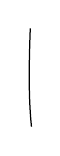
\begin{tikzpicture}[x=1cm,y=1cm]
\draw[line width=.45pt] (0,1.25) .. controls (-.015,.82) and (-.025,.40) .. (.015,0);
\end{tikzpicture}}

Pour le montrer, on va plonger
$\Pi_{0,3}$ comme sous-groupe d'indice fini
dans $\Pi'_{0,3}$, d'où un plongement \unsure{analogue}
\deleted{\illegible{1}}
\[
(2)\qquad\widehat{\Pi}_{0,3}\lhook\joinrel\longrightarrow\widehat{\Pi}'_{0,3}
\]
qui sera compatible avec l'action ext. de $\Gamma$.

\scanpage{507}

Considérons pour cela le schéma quotient
\[
Y=\underbrace{\mathbb P^1_{\mathbb Q}}_{X}/\unsure{\mathfrak S_3}
\]
avec les trois points \inserted{$a_0,a_1,a_\infty$} de $Y$, rationnels sur
$\mathbb Q$, \inserted{$a_0$} correspondant à la trajectoire
\deleted{des} $\{0,1,\infty\}$, $a_1$ à la trajectoire
$\{-1,\frac12,2\}$, et $a_\infty$ à la trajectoire
$\{\unsure{-j},\unsure{-\overline j}\}$ de $\unsure{\mathfrak S_3}$
\margin{$j=\exp\frac{2i\pi}{3}$}
(ce qui épuise \unsure{l'ens} des trajectoires
``singulières'' géométriques). On sait que $Y$ est une droite projective
(sur $\overline{\mathbb Q}$ a priori), \unsure{qu'on} \unsure{épingle} par
$a_0,a_1,a_\infty$ comme points $0,1,\infty$, \unsure{(donc}
$Y\simeq\mathbb P^1_{\mathbb Q}$ -- le \deleted{\illegible{1}} morphisme
$X\longrightarrow Y$ s'identifie donc à un morphisme bien déterminé
\[
(3)\qquad
f:\begin{array}{ccc}
\mathbb P^1_{\mathbb Q}&\longrightarrow&\mathbb P^1_{\mathbb Q}\\
\Vert&&\Vert\\
X&&Y
\end{array}
\]
\deleted{(en fait, $f$ peut se définir comme morphisme
$\mathbb P^1_{\mathbb Z}\longrightarrow\mathbb P^1_{\mathbb Z}$,
mais ici peu nous importe)}
qui fait de $X$ un \unsure{revêtt|revêtement} galoisien de $Y$, de groupe
$\unsure{\mathfrak S_3}$, étale \unsure{au|en} dessus de
$\mathbb P^1_{\mathbb Q}\setminus\{0,1,\infty\}$, avec comme indices de
ramification en ces points $2,2,3$. Du point de vue de la géométrie des cartes
(\unsure{se plaçant|se plongeant} sur le corps de base $\mathbb C$), on considère la

\scanpage{508}
\mspage{\unsure{258 (259)}}

carte déterminée sur $X$ par les triangles sphériques $(0,1,\infty)$
(sur l'axe réel comme équateur) -- qui est donc la carte triangulaire
\unsure{pondérée} universelle -- comme image inverse de la carte universelle
(ayant un seul sommet $0$, une seule arête (repliée) $0\longrightarrow1$,
une seule face, de centre $\infty$).
\margin{\figure{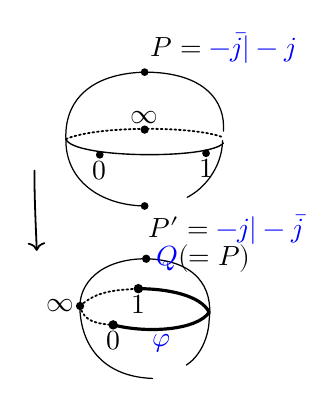
\begin{tikzpicture}[x=1cm,y=1cm,line cap=round,line join=round]
\draw[line width=.45pt] (0,2.85)
 .. controls (-.71,2.83) and (-1.02,2.47) .. (-1,2)
 .. controls (-1.01,1.48) and (-.57,1.16) .. (0,1.15);
\draw[line width=.45pt] (0,2.85)
 .. controls (.76,2.85) and (1.03,2.48) .. (1,2.10);
\draw[line width=.45pt] (.99,1.98)
 .. controls (.98,1.62) and (.74,1.36) .. (.54,1.26);
\draw[line width=.5pt] (-1,2)
 .. controls (-.91,1.75) and (.83,1.74) .. (1,1.95);
\draw[densely dotted,line width=.65pt] (-1,2)
 .. controls (-.61,2.17) and (.63,2.17) .. (1,2.02);
\fill (0,2.85) circle (1.4pt);
\node[anchor=south west,inner sep=2pt] at (0,2.88) {$P=\unsure{-\bar j|-j}$};
\fill (0,1.15) circle (1.4pt);
\node[anchor=north west,inner sep=2pt] at (-.03,1.12) {$P'=\unsure{-j|-\bar j}$};
\fill (-.57,1.80) circle (1.4pt);
\node[below,inner sep=2pt] at (-.57,1.80) {$0$};
\fill (.78,1.82) circle (1.4pt);
\node[below,inner sep=2pt] at (.78,1.82) {$1$};
\fill (0,2.12) circle (1.5pt);
\node[above,inner sep=2pt] at (0,2.12) {$\infty$};
\draw[->,line width=.65pt] (-1.40,1.60)
 .. controls (-1.40,1.22) and (-1.38,.85) .. (-1.37,.58);
\draw[line width=.45pt] (.02,.48)
 .. controls (-.55,.48) and (-.86,.17) .. (-.82,-.20)
 .. controls (-.78,-.70) and (-.46,-1.02) .. (.10,-1.04);
\draw[line width=.45pt] (.02,.48)
 .. controls (.65,.46) and (.87,.12) .. (.82,-.29)
 .. controls (.81,-.58) and (.66,-.79) .. (.53,-.87);
\fill (.02,.48) circle (1.5pt);
\node[anchor=west,inner sep=2pt] at (.07,.48) {$\unsure{Q}(=P)$};
\fill (-.82,-.12) circle (1.5pt);
\node[left,inner sep=2pt] at (-.82,-.12) {$\infty$};
\fill (-.08,.10) circle (1.7pt);
\node[below,inner sep=2pt] at (-.08,.10) {$1$};
\fill (-.40,-.36) circle (1.7pt);
\node[below,inner sep=2pt] at (-.40,-.36) {$0$};
\draw[line width=1.15pt] (-.08,.10)
 .. controls (.28,.10) and (.71,.02) .. (.82,-.20)
 .. controls (.66,-.43) and (.03,-.47) .. (-.40,-.36);
\draw[densely dotted,line width=.65pt] (-.82,-.12)
 .. controls (-.60,.08) and (-.36,.08) .. (-.08,.10);
\draw[densely dotted,line width=.65pt] (-.82,-.12)
 .. controls (-.78,-.32) and (-.59,-.35) .. (-.40,-.36);
\node[below,inner sep=1pt] at (.22,-.44) {$\unsure{\varphi}$};
\end{tikzpicture}}}
Tout revêtement \deleted{\unsure{de}} \inserted{étale} topologique de
$U_{03}(\mathbb C)\subset X$ donne ainsi un rev. étale topologique de
$U_{0,3}(\mathbb C)\subset Y$, \deleted{ramifié} ayant au
\deleted{\illegible{1}} \inserted{dessus de} $1$ la ramification $2$,
au dessus de $\infty$ la ramification $3$ \unsure{exactt|exactement},
ce qui correspond au foncteur ``oubli'' \inserted{(de la pondération)},
où une carte triangulaire \unsure{pondérée} est considérée comme une carte
tout court. Du point de vue des groupes fondamentaux \unsure{on} trouve
ainsi une \deleted{\unsure{hom.} de groupes extérieurs}
\inserted{équiv. de catégories}

\diagram{\begin{tikzcd}[ampersand replacement=\&,column sep=large,row sep=huge]
\&
\deleted{\begin{gathered}
\Pi_1(\unsure{X(\mathbb C)}\setminus\{0,1,\infty\})\\[-2pt]
\rotatebox{90}{$=$}\\[-2pt]
\Pi_{0,3}
\end{gathered}}
\arrow[r,phantom,"{\deleted{\longleftarrow}}" description]
\&
\deleted{\begin{gathered}
\Pi_1\!\left(Y(\mathbb C)\setminus\{0,1,\infty\};
\underbrace{2\{1\}+3\{\infty\}}_{\substack{\text{signature de}\\\text{ramification}}}\right)\\[-2pt]
\rotatebox{90}{$=$}\\[-2pt]
\Pi'_{0,3}
\end{gathered}}
\\
(\deleted{\illegible{1}}\inserted{4}) \&
\left(\text{Rev. étales de }X\setminus\{0,1,\infty\}=U_{0,3}\right)
\arrow[r,phantom,"\simeq" description]
\arrow[d,phantom,"{\rotatebox{-90}{$\simeq$}}" description]
\&
\begin{gathered}
\left[\begin{gathered}
\text{Rev. de }Y\setminus\{0,1,\infty\}=U_{0,3}\\
\text{avec ramification sub. à}\\
\text{la signature }2\{1\}+3\{\infty\}
\end{gathered}\right]\\
\big/\begin{gathered}
\text{l'objet }(X\setminus\{0,1,\infty\})\\
\text{de la dite catégorie}
\end{gathered}
\end{gathered}
\arrow[d,phantom,"{\rotatebox{90}{$\simeq$}}" description]
\\
\& \Pi_{0,3}\text{-ensembles} \&
(\Pi'_{0,3}\text{-Ens})/\deleted{\unsure{E}}E
\end{tikzcd}}

où $E$ est le $\Pi'_{0,3}$-ens. correspondant à l'objet
$X\setminus\{0,1,\infty\}$ de la cat. des rev. étales de
$\unsure{Y\setminus\{0,1,\infty\}}$ à ramification
\deleted{\unsure{imposée}}\inserted{\unsure{subordon-}}née à
$2\{1\}+3\{\infty\}$

\deleted{$\unsure{\simeq}\ \unsure{\Pi_{0,3}^{\prime\circ}}\in\mathrm{Ens}$}

\scanpage{509}
\mspage{\unsure{260|250}}

Ici, \deleted{\illegible{3}} \inserted{\deleted{\illegible{1}} le point base de $Y-\{0,1,\infty\}$ choisi\unsure{;|,} \unsure{pour} décrire les} revêtements \deleted{$E=\unsure{f^{-1}}\unsure{(}$} (à ramification \unsure{subordonnée} à \dots) par un groupe fondamental à ramification, étant \unsure{encore} $P=-\bar j$, on aura
\[
(5)\qquad E=f_{\unsure{\mathbf C|\mathbb C}}^{-1}(P)
\]
et on peut expliciter ainsi la cat. $(\Pi'_{03}\text{-Ens})/E$\unsure{;}

Où $E$ est un espace homogène, \inserted{\unsure{isom. au}} \unsure{quot.} de $\Pi'_{03}$ par le \unsure{ss-groupe|s-groupe} \inserted{$\Pi'^{\circ}_{03}$} noyau de l'hom. surjectif \inserted{idoine}
\[
(6)\qquad
\left\{
\begin{array}{l}
\Pi'_{0,3}\longrightarrow\unsure{\mathfrak S_3|\mathcal S_3}\\[2pt]
\left.
\begin{array}{lll}
\ell_0 &\longmapsto& \text{él. d'ordre 2}\\
\ell_1 &\longmapsto& \text{él. d'ordre 2}\\
\ell_\infty &\longmapsto& \text{\unsure{él.} d'ordre 3}
\end{array}
\right)\quad\text{à calculer !}
\end{array}
\right.
\]

On choisit un $Q_0\in E$ comme ``origine'' de $E$ -- pour pouvoir identifier $E$ comme $\Pi'_{0,3}$-ens à $\Pi'_{03}/\Pi'^{\circ}_{03}\simeq\unsure{\mathfrak S_3}$ -- alors $(\mathrm{Ens}\,\Pi'_{03})/E$ s'identifie, par le foncteur $F\longmapsto F_{Q_0}$, à $\mathrm{Ens}(\Pi'^{\circ}_{03})$.

On trouve donc en résumé une équivalence de catégories (dépendant du choix de $Q_0$)
\[
\Pi_{03}\text{-ens}\quad\unsure{\simeq}\quad\Pi'^{\circ}_{03}\text{-ensembles}
\]
qui est elle-même décrite par un bitorseur sous $(\Pi'^{\circ}_{0,3},\Pi_{03})$ -- et, à isom \deleted{que} (non unique !) près, par un isomorphisme
\[
\Pi_{03}\simeq\Pi'^{\circ}_{0,3}\quad -
\]
les isomorphismes ainsi obtenus (pour des

\scanpage{510}
\mspage{\unsure{249}}

origines variables du bitorseur) \unsure{forment|formant} exactement une classe de conjugaison par $\Pi'^{\circ}_{03}$ -- i.e. un \uline{\unsure{isom.}} \uline{extérieur} $\Pi_{03}\simeq\Pi'^{\circ}_{03}$. Quand de plus le choix de $Q_0$ varie, on trouve \deleted{comme} un \unsure{composé|composés}
\[
\Pi_{0,3}\longrightarrow\Pi'^{\circ}_{03}\longrightarrow\Pi'_{03}
\]
\deleted{\unsure{exactement}} une classe de $\Pi'_{03}$-conj, i.e. un hom extérieur.

J'ai beaucoup \unsure{turbiné} pour pas grand chose -- à défaut d'avoir écrit les \unsure{fonctorialités} \inserted{générales} \unsure{nécessaires|élémentaires} pour les ``groupes fondamentaux \unsure{avec} ramification''. \unsure{P.ex.} le bifoncteur $I$ mystérieux de tantôt est formé des \unsure{classes} de chemins de $P\in\unsure{X(\mathbb C)|X_{\mathbb C}}\setminus\{0,1,\infty\}$ (point base pour calculer $\Pi_{0,3}$) vers $Q_0$ (jouant le rôle d'un nouveau pt base, ayant le mérite de s'envoyer sur celui \inserted{-- $P$ --} qui sert à calculer $\Pi'_{03}$, groupe fondamental à ramification sur $Y(\mathbb C)\setminus\{0,1,\infty\}$ \dots) Il serait peut-être plus commode de définir \unsure{direct\textsuperscript{t}|directement} un foncteur en sens inverse\unsure{:|.}
\[
(7)\qquad
\begin{array}{c}
\text{Rev. de }Y(\mathbb C)\inserted{\setminus(0,1,\infty)}\ \text{subordonnés}\\
\text{à la signature }2\{1\}+3\{\infty\}
\end{array}
\longrightarrow
\begin{array}{c}
\text{Rev. \unsure{ét.les|étales} de}\\
X(\mathbb C)\setminus\{0,1,\infty\}
\end{array}
\]
par image inverse, \unsure{suivi|suivie} d'une \uline{normalisation}
\scanpage{511}
\mspage{261}

-- Ici on utilise le fait que l'objet $X(\mathbb C)\setminus\{0,1,\infty\}$ de la catégorie des \unsure{rev\textsuperscript{ts}} à ramification maximum \unsure{imposé|imposée}, réalise justement un maximum, en les pts $1,\infty$ où la condition intervient.
On trouve que le foncteur correspondant
\[
\tag{7 bis}
\Pi'_{03}\text{-}\mathrm{Ens}\longrightarrow(\Pi_{0,3}\text{-}\mathrm{Ens})
\]
a les propriétés d'exactitude d'un foncteur associé à un morphisme de topos galoisiens
\diagram{\begin{tikzcd}[ampersand replacement=\&]
\overset{\inserted{\unsure{B}}}{\unsure{B|D}}_{\Pi_{03}} \arrow[r] \& B_{\Pi'_{0,3}}
\end{tikzcd}}
(\unsure{commute aux} $\underset{\longrightarrow}{\lim}$ \unsure{quelc.}, exact à g.) et est donc défini par un $(\Pi_{03}^{\deleted{\unsure{\wedge}}},\Pi'_{03})$ ens. qui soit un torseur (à droite) pour $\Pi'_{03}$. Le choix d'une origine pour ce torseur définit alors aussi un hom correspondant $\Pi_{0,3}\longrightarrow\Pi'_{03}$.

\margin{Ce bitorseur est aussi l'ens. des ($Y(\mathbb C)\setminus$\deleted{\illegible{2}}\inserted{\unsure{$\{0\}$}}) \unsure{isom|hom} des ``rev. universel à \unsure{ramification} imposée'' de cet espace, sur le rev. universel \deleted{\unsure{à ramification}} \deleted{\unsure{ordinaire}} ordinaire de $X(\mathbb C)\setminus\{0,1,\infty\}$ \ldots}

Revenons à la situation arithmétique sur $\mathbb Q$, où on dispose non seulement des groupes fondamentaux géom. profinis $\widehat{\Pi}_{03}$, $\widehat{\Pi}'_{03}$, mais aussi d'extensions
\[
\tag{8}
\left\{\begin{aligned}
1&\unsure{\longrightarrow}\widehat{\Pi}_{03}\longrightarrow\mathcal E_{0,3}^{\deleted{\unsure{\wedge}}}\longrightarrow\Gamma_{\deleted{\unsure{\mathbb Q}}}\longrightarrow1\\
1&\unsure{\longrightarrow}\widehat{\Pi}'_{03}\unsure{\longrightarrow}\mathcal E_{0,3}^{\prime\deleted{\unsure{\wedge}}}\unsure{\longrightarrow}\Gamma\unsure{\longrightarrow}1
\end{aligned}\right.,
\]
s'interprétant comme des groupes fondamentaux de $\unsure{U}_{03\deleted{\mathbb Q}}$, resp. de $\unsure{U}_{03}$ avec ramification imposée $2\{1\}+3\{\infty\}$. Les raisonnements

\scanpage{512}

précédents s'étendent à ce cadre, et fournissent donc un homomorphisme \deleted{extérieur} \inserted{d'extensions}
\diagram{\begin{tikzcd}[ampersand replacement=\&]
1 \arrow[r] \& \widehat{\Pi}_{03} \arrow[r] \arrow[d] \& \mathcal E_{03} \arrow[r] \arrow[d] \& \Gamma \arrow[r] \arrow[d,equal] \& 1 \\
1 \arrow[r] \& \widehat{\Pi}'_{03} \arrow[r] \& \mathcal E'_{03} \arrow[r] \& \Gamma \arrow[r] \& 1
\end{tikzcd}\quad(9)},
modulo conjugaison par un autom. int. de $\Pi'_{03}$.

\margin{(9 bis) $\widehat{\Pi}_{0,3}\longrightarrow\widehat{\Pi}'_{0,3}$ s'insère dans une suite exacte
\[
\boxed{1\longrightarrow\widehat{\Pi}_{0,3}\longrightarrow\widehat{\Pi}'_{0,3}\longrightarrow\unsure{\mathfrak S}_3\longrightarrow1}
\]
et itou pour les groupes discrets
\[
\boxed{1\longrightarrow\Pi_{0,3}\longrightarrow\Pi'_{0,3}\longrightarrow\unsure{\mathfrak S}_3\longrightarrow1}.
\]}

Ceci dit, soit $K$ le noyau de l'opération extérieure de $\Gamma$ sur $\Pi'_{03}$. On voit alors que \deleted{$K$ opère} l'opération ext. de $K$ sur le sous-groupe ouvert $\widehat{\Pi}_{03}$ se fait par un groupe fini (en fait, par \inserted{l'intermédiaire de} $\widehat{\Pi}'_{03}/\widehat{\Pi}_{03}\simeq\unsure{\mathfrak S}_3$ \ldots) -- ce qui implique, par le th. 1 du \S\ précédent, que le groupe $K$ lui-$\overline{\mathrm m}$ est fini. Donc par Artin on a $K=1$ ou $K=(1,\tau)$, $\tau$ la conjugaison complexe. Mais comme $\chi(\tau)=-1$ il est évident que l'op. ex. de $\tau$ sur $\Pi'_{03}$ \inserted{(ni $\overline{\mathrm m}$ sur $(\Pi'_{03})_{\unsure{\mathrm{ab}}}^{*}$ \deleted{\illegible{2}})} n'est pas triviale\ldots
\margin{$*\simeq\unsure{\mathbb Z/2\mathbb Z+\mathbb Z/3\mathbb Z}$}
\deleted{\unsure{Ce qui}} Cela prouve la proposition.

\scanpage{513}
\mspage{262}

J'ai envie maintenant d'interpréter $\Pi_{03}^{\unsure{\prime}}$ comme $\mathcal T^+_{1,1}/\deleted{\text{sous-groupe}}\inserted{\text{centre}}$ (isom. \unsure{à} $\{\pm1\}$\unsure{),|,} et itou pour $\widehat{\Pi}'_{03}\simeq\widehat{\mathcal T}_{11}/\{\pm1\}$, \unsure{isomorphisme|isomorphismes} qui soit compatible à l'action extérieure de $\Gamma$, On a (pour mémoire)
\[
\tag{10}
\mathcal T_{1,1}\xrightarrow{\sim}\mathrm{Gl}(2,\mathbb Z),
\]
l'isomorphisme étant obtenu ainsi :
\[
\tag{11}
\mathcal T_{1,1}\xrightarrow[\substack{\text{bouchage}\\\text{du trou}}]{\mathrm{iso}}\mathcal T_{1,0}\xrightarrow{\mathrm{iso}}\mathrm{Autext}\left(\underbrace{\Pi_{10}}_{\substack{\wr\\\mathbb Z^2}}\right)\simeq\mathrm{Gl}(2,\mathbb Z)
\]

On a donc
\[
\tag{12}
\mathcal T^+_{11}\simeq\mathrm{Sl}(2,\mathbb Z)
\]
et
\[
\tag{13}
\mathrm{Cent}(\mathcal T_{11})\simeq(\pm1)
\]
(s'identifie au ss-groupe des homothéties de $\mathrm{Sl}(2,\mathbb Z)$). Il est connu qu'on a \unsure{dans} $\mathrm{Sl}(2,\mathbb Z)/(\pm1)$ deux générateurs $\unsure{\lambda_3,\lambda_2}$, satisfaisant respectivement
\[
\tag{14}
\lambda_3^3=1,\quad\lambda_2^2=1
\]
et tels que ces relations soient une \uline{présentation} de $\mathrm{Sl}(2,\mathbb Z)/(\pm1)$. Sauf erreur, ces \unsure{élts|élmts} proviennent d'\unsure{élts|élmts} $u_6,u_4$ de $\mathrm{Sl}(2,\mathbb Z)$ lui-$\overline{\mathrm m}$, satisfaisant
\[
\tag{15}
u_6^6=1,\quad u_4^4=1
\]

\scanpage{514}

et qui correspondent aux seuls éléments d'ordre 6 et d'ordre 4 (à conjugaison et passage à l'inverse près). En fait, \unsure{tout} élément d'ordre fini de $\mathrm{Sl}(2,\mathbb Z)$ est conjugué à une puissance \unsure{de|d'} \deleted{un} $u_4$, ou $u_6$. Les \unsure{ss/groupes} \unsure{engendrés} resp. par $u_4$ et $u_6$, cycliques d'ordre 4 et 6, sont les groupes des \unsure{autom.} des deux courbes elliptiques exceptionnelles (dites ``\unsure{anharmoniques}'') (en car. 0).

\deleted{Pour} Je n'ai pas de formule sous la main pour ``placer'' \deleted{\unsure{$u_4$}} $u_4$ et $u_6$, de façon qu'ils engendrent le groupe $\mathrm{Sl}(2,\mathbb Z)$\deleted{\unsure{$/\pm1$}} \unsure{mod} son centre (ce qui implique sans doute qu'ils engendrent $\mathrm{Sl}(2,\mathbb Z)$ --- mais \unsure{on fera attention|enfin. Attention} à la relation supplémentaire. \deleted{s'ajoutant \unsure{à} \inserted{(15)} \unsure{des} relations fondamentales}
\[
(16)\qquad u_4^2=u_6^3\qquad\unsure{\varepsilon}
\]
(c'est \deleted{\illegible{2}} \unsure{justement} l'élément $-1$ du centre de $\mathrm{Sl}(2,\mathbb Z)$). Je n'en ai peut-être pas besoin (de la formule explicite pour $u_4,u_6$). On \unsure{définira|définit} alors

\scanpage{515}
\mspage{263}

\[
(17)\qquad \Pi'_{03}\xrightarrow{\sim}\mathrm{Sl}(2,\mathbb Z)/(\pm1)
\]
par
\[
(18)\qquad
\begin{array}{rcl}
\ell'_1&\longmapsto&\lambda_2\\
\ell'_\infty&\longmapsto&\lambda_3
\end{array}
\]
\[
\bigl[\text{donc}\qquad\ell'_0\longmapsto(\lambda_3\lambda_2)^{-1}
=\lambda_2\lambda_3^{-1}=\lambda_2\lambda_3^2\bigr],
\]
\unsure{où} $\ell'_0,\ell'_1,\ell'_\infty$ sont les générateurs de $\Pi'_{03}$ correspondants à ceux $\ell_0,\ell_1,\ell_\infty$ de $\Pi_{03}$, avec les relations de définition
\[
(19)\qquad\ell'_\infty\ell'_1\ell'_0=1\qquad
\ell_1^{\prime 2}=1,\quad\ell_\infty^{\prime 3}=1
\]
de sorte que $\Pi'_{03}$ est bien le groupe \deleted{libre} de générateurs $\ell'_1,\ell'_\infty$ satisfaisant à : $\ell_1^{\prime 2}=1,\ell_\infty^{\prime 3}=1$.

Je veux maintenant me convaincre que l'homomorphisme correspondant à (17)
\[
(20)\qquad\widehat{\Pi}'_{03}\longrightarrow
\mathrm{Sl}(2,\mathbb Z)^\wedge/\pm1\simeq
\widehat{\mathcal T}_{1,1}^{+}/(\pm1)
\]
est compatible avec l'opération extérieure de $\Gamma=\Pi_{\mathbb Q}$. Pour ceci, j'ai envie de définir directement le composé \unsure{avec} $\unsure{\widehat{\Pi}_{0,3}|\Pi_{0,3}}\longrightarrow\widehat{\Pi}'_{03}$
\[
\text{\deleted{\unsure{(21)}}}\qquad\widehat{\Pi}_{03}\longrightarrow\widehat{\mathcal T}_{1,1}^{+}/\pm1
\]
et $\overline{\mathrm m}$ de le \unsure{relever} en un hom
\[
(21)\qquad\widehat{\Pi}_{03}\longrightarrow\widehat{\mathcal T}_{11}^{+}\;.
\]

\scanpage{516}

Au niveau des groupes discrets, on définit bien
\[
(22)\qquad\Pi_{03}\longrightarrow\mathrm{Sl}(2,\mathbb Z)
\]
\[
\left\{
\begin{array}{rcl}
\ell_1&\longmapsto&u_4\\
\ell_\infty&\longmapsto&u_6\\
\ell_0&\longmapsto&(u_6u_4)^{-1}=u_4^{-1}u_6^{-1}
\end{array}
\right.
\]
et $\mathrm{Sl}(2,\mathbb Z)$\inserted{$\simeq\mathcal T_{11}^{+}$} s'identifie au quotient de $\Pi_{0,3}$ par le \unsure{sous-groupe} invariant \unsure{engendré} par les éléments
\[
\ell_1^4,\ \ell_\infty^6,\ (\ell_1^2)(\ell_\infty^3)^{-1}\;.
\]

D'ailleurs $\Pi_{03}$ peut s'interpréter comme un groupe de Teichmüller $\mathcal T_{0,4}^{!+}$, et (22) comme un hom
\margin{en effet, $\mathcal T_{g,\nu}^{!}$ est ext. de $\mathcal T_{g,\nu-1}^{!}$ par $\Pi_{g,\nu-1}$ (si $(g,\nu-1)$ \unsure{anab.}) et itou pour les $\mathcal T^{+}$, $\mathcal T_{0,3}^{!+}=(1)$ !}
\[
\text{\deleted{\unsure{(24)}}}\ (23)\qquad\mathcal T_{0,4}^{!+}\longrightarrow\mathcal T_{11}^{+}
\]
dont je soupçonne qu'il se prolonge en un hom
\[
(24)\qquad
\diagram{\begin{tikzcd}[ampersand replacement=\&,column sep=large]
\mathcal T_{0,4}^{!}\arrow[r]\arrow[d,phantom,"\wr" description]\&\mathcal T_{11}\arrow[d,phantom,"\wr" description]\\
\begin{gathered}
\text{ext. de }\{1,\unsure{\tau}\}\text{ par}\\
\Pi_{0,3},\ \text{qui n'est}\\
\text{autre que le}\\
\text{groupe cartographique}\\
\text{triangulé pondéré}\\
\text{non orienté}
\end{gathered}
\&\mathrm{Gl}(2,\mathbb Z)
\end{tikzcd}}
\]
\margin{pas encore défini}

J'interprète le premier \unsure{mb} \inserted{de (23)} comme le $\Pi_1$ ``géométrique transcendant'' \unsure{des|du} topos \unsure{modulaires|modulaire}

\scanpage{517}
\mspage{264}

$\mathbb{M}_{0,4}^{!}$, classifiant les \deleted{courbes rationnelles} \inserted{droites projectives} avec quatre points distincts numérotés de $1$ à $4$ ; et le deuxième \unsure{mb|md} de (23) est le $\pi_1$ transcendant du topos modulaire $M_{1,1}$, classifiant les courbes elliptiques (avec une origine fixée). On devrait donc pouvoir définir, au niveau des \deleted{schémas} multiplicités modulaires sur $\mathbb{Q}$
\[
(25)\qquad (\mathbb{M}_{0,4}^{!})_{\mathbb{Q}} \longrightarrow
(\mathbb{M}_{1,1}^{\deleted{\unsure{!}}})_{\mathbb{Q}}
\]
qui donnerait naissance à (23). \deleted{Cela \unsure{signifie aussi}}

Mais on voit de suite qu'on a un isom can.
\[
(26)\qquad \mathbb{M}_{0,4}^{!}\simeq U_{0,3}
\]
(je laisse tomber les indices $\mathbb{Q}$), et la donnée de (25) revient donc aussi à la donnée d'une famille de courbes elliptiques sur $U_{0,3}$.

Mais \unsure{si} $\lambda$ est la \unsure{``variable'' $\in U_{0,3}$''}, en prenant ``le'' rev. quadratique $E_\lambda$ de \deleted{\illegible{1}} $\mathbb{P}^1$ ramifié en $0,1,\infty,\lambda$,

\scanpage{518}

on trouve une courbe elliptique, avec quatre points marqués \deleted{resp.} au dessus de $0,1,\infty,\lambda$ --- dont on peut prendre le pt au dessus de $0$ comme origine --- alors les autres points sont les trois points d'ordre $2$, indexés resp. par $1,\infty,\lambda$.

De façon plus précise : sur un schéma de base quelconque \inserted{$S$}, sauf que $2$ y soit inv (car. résid. \unsure{ttes} $\ne 2$), \deleted{le} \inserted{on a un} foncteur qui va \deleted{des} \inserted{de la cat des syst $(E,\alpha,\beta\deleted{,\unsure{\gamma}})$ d'une} \unsure{courbes|courbe} \unsure{elliptiques|elliptique} (\unsure{homogène|homogènes}) \unsure{relative|relatives} \deleted{\unsure{avec} \illegible{1}} sur $S$, et \deleted{\unsure{dont}} $\alpha,\beta\deleted{,\unsure{\gamma}}$ \deleted{trois} \inserted{deux} sections de $E$ qui forment une base de ${}_2E$ \unsure{en tant} que schéma \inserted{loc. constant} en $\mathbb{F}_2$-Modules (un système local de $\mathbb{F}_2$-modules) de $S$ [\unsure{donnant} naissance à : $\gamma=\alpha+\beta$, comme un troisième larron --- de sorte que $(\beta,\gamma)$\unsure{,|.} \deleted{et \unsure{$(\gamma,\alpha)$}} \inserted{etc} sont en fait aussi des bases) --- vers la catégorie des fibrés en droites projectives $P$ sur $S$, avec quatre sections \inserted{$u_0,u_1,u_\infty,\lambda$} \unsure{marquées} distinctes en chaque point, en associant à $E$ le quotient $E/\pm1$, \unsure{muni} des sections $u_0,u_1,u_\infty,\lambda$ qui sont image resp. de $0,\alpha,\beta,\gamma=\alpha+\beta$

\margin{il revient au $\overline{\mathrm m}$ de dire que \unsure{l'on a|les} trois sections $\alpha,\beta,\gamma$ de ${}_2E$ sur $S$, qui \unsure{sont} $\forall s\in S$, \deleted{\unsure{partout}} distinctes et \unsure{partant|partout} $\ne1$.}

\scanpage{519}
\mspage{265}

\margin{Les pages qui suivent sont inutilement compliquées, avec l'introduction des $\unsure{M|\mathbb M}'_{1,1}$, $\mathcal{T}'_{1,1}$ \unsure{etc.} -- il suffit d'y aller \unsure{brutalement|bonnement} avec la courbe elliptique $y^2=\sqrt{x(x-1)(x-\lambda)}$, sur $U_{0,3}$, \unsure{pour} \illegible{1} \unsure{avoir} $U_{0,3}\longrightarrow \unsure{M|\mathbb M}_{1,1}$ cf plus bas\ldots}

et ce foncteur est \uline{presque} une équivalence de catégories. Ce qui lui manque pour l'être, c'est que pour une courbe elliptique relative $E$, la symétrie \inserted{$x\mapsto -x$} de $E$ -- qui est un autom. non trivial -- opère \unsure{trivialement} sur l'objet correspondant $E/\pm1$. Donc il \unsure{faut} prendre \unsure{la|le} \deleted{catégorie fibrée} \inserted{champ} sur $(\mathrm{Sch})$, déduit de celle des courbes elliptiques en commençant par prendre $\unsure{\mathrm{Isom}}(E,F)'=\unsure{\mathrm{Isom}}(E,F)/\pm1$, puis on prendra le champ associé à un préchamp (les objets sur $S$ sont les ``courbes elliptiques relatives à symétrie près sur $S$''). \unsure{Cet|Ce|Le} champ est représentable par une multiplicité modulaire $\unsure{M|\mathbb M}'_{1,1}$, \deleted{\unsure{déduit de} \illegible{1}} ayant comme groupe fondamental géom. $\mathrm{Sl}(2,\mathbb{Z})^{\wedge}/\pm1$ justement, déduit \deleted{des} p.ex. des variétés modulaires à rigidification de Jacobi d'échelon $n$, $\unsure{M|\mathbb M}_{11}[n]$ -- avec groupe $\mathrm{Sl}(2,\mathbb{Z}/n\mathbb{Z})$ opérant dessus, de sorte que
\[
 (27)\qquad \unsure{M|\mathbb M}_{11}\simeq \bigl(\unsure{M|\mathbb M}_{1,1}[n],\mathrm{Sl}(2,\mathbb{Z}/n\mathbb{Z})\bigr)
\]
\unsure{en outre|on note} que \inserted{le ss-groupe central $\unsure{(\pm1)|\{\pm1\}}$ de} $\mathrm{Sl}(2,\mathbb{Z}/n\mathbb{Z})$ opère \unsure{trivialement} sur $\unsure{M|\mathbb M}_{11}[n]$, donc on peut faire opérer le groupe quotient $\mathrm{Sl}(2,\mathbb{Z}/n\mathbb{Z})'\,\deleted{\illegible{1}}=\mathrm{Sl}(2,\mathbb{Z}/n\mathbb{Z})/\pm1$, et poser

\scanpage{520}

\[
 (28)\qquad \unsure{M|\mathbb M}'_{11}=\bigl(\unsure{M|\mathbb M}_{11}[n],\mathrm{Sl}(2,\mathbb{Z}/n\mathbb{Z})'\bigr)
\]
\unsure{(ce|Ce} qui \unsure{manifest$^{\mathrm t}$|manifestement} ne dépend pas du choix de $n$, $n\geq2$). On trouve ainsi un homomorphisme
\[
 (29)\qquad
 \diagram{\begin{tikzcd}[ampersand replacement=\&,row sep=small]
 \unsure{M|\mathbb M}^!_{0,4} \arrow[r] \arrow[d,equal] \& \unsure{M|\mathbb M}'_{11} \\
 U_{0,3} \&
 \end{tikzcd}}
\]
qui fait de $\unsure{M|\mathbb M}^!_{0,4}$ un rev. galoisien de groupe $\unsure{\mathfrak{S}_3}$ de $\unsure{M|\mathbb M}'_{11}$, et de façon plus précise
\[
 (30)\qquad
 \diagram{\begin{tikzcd}[ampersand replacement=\&,column sep=large]
 \unsure{M|\mathbb M}^!_{0,4} \arrow[r,dash,"\sim"] \&
 \unsure{M|\mathbb M}_{1,1}^{\prime\,\deleted{\illegible{1}}}[2]
 \arrow[r,"{\text{rev. galoisien de groupe }\mathrm{Sl}(2,\mathbb{F}_2)\simeq\unsure{\mathfrak{S}_3}}"'] \&
 \unsure{M|\mathbb M}'_{11}\,\deleted{\illegible{1}}
 \end{tikzcd}}
\]
le groupe fondamental géom. de $\unsure{M|\mathbb M}_{11}[2]$ \unsure{étant} d'ailleurs isomorphe au noyau de \inserted{l'hom} $\mathrm{Sl}(2,\mathbb{Z})^{\prime\wedge}\longrightarrow\mathrm{Sl}(2,\mathbb{Z}/2\mathbb{Z})$ qui factorise l'hom canonique $\mathrm{Sl}(2,\mathbb{Z})^{\wedge}_{\deleted{\illegible{1}}}\longrightarrow\mathrm{Sl}(2,\mathbb{Z}/2\mathbb{Z})$.

Passant aux groupes fondamentaux pour $\unsure{M|\mathbb M}^!_{0,4}=U_{0,3}$ et $\unsure{M|\mathbb M}'_{11}$, on trouve un \unsure{hom|homom.} de suites exactes

\deleted{\unsure{(31)}}
\[
 (31)\qquad
 \diagram{\begin{tikzcd}[ampersand replacement=\&,column sep=small,row sep=small]
 \& \inserted{\unsure{\mathcal{T}_{0,4}^{!+}|\widehat{\mathcal{T}}_{0,4}^{!+}}}
   \arrow[d,phantom,"\inserted{\Vert}" description]
 \& \inserted{\unsure{N_{0,4}|\mathcal{N}_{0,4}}}
   \arrow[d,phantom,"\inserted{\Vert}" description] \& \& \\
 1 \arrow[r] \& \widehat{\Pi}_{0,3} \arrow[r] \arrow[d]
 \& \mathcal{E}_{0,3} \arrow[r] \arrow[d]
 \& \Gamma \arrow[r,dash] \arrow[d,"\Vert"] \& 1 \\
 1 \arrow[r] \& \widehat{\mathcal{T}}_{1,1}^{\prime+} \arrow[r]
   \arrow[d,phantom,"\inserted{\wr}" description]
 \& \mathcal{E}'_{11} \arrow[r] \& \Gamma \arrow[r] \& 1 \\
 \& \inserted{\widehat{\mathcal{T}}_{11}^{+}/\unsure{\{\pm1\}|(\pm1)}
   \simeq\mathrm{Sl}(2,\mathbb{Z})^{\wedge}/\pm1} \& \& \&
 \end{tikzcd}}
\]
\scanpage{521}
\mspage{266}

qui identifie $\mathcal E_{0,3}$ à un ss-groupe \inserted{\unsure{ouvert}\illegible{1}} d'indice $6$ de $\mathcal E'_{1,1}=\mathcal E_{1,1}/(\pm1)$, et itou pour $\widehat\Pi_{0,3}$ dans $\widehat{\mathcal T}_{1,1}^{\prime+}$. On trouve ainsi un iso\deleted{\illegible{1}}morphisme
\[
(32)\qquad
\widehat\Pi_{0,3}\xrightarrow{\sim}
\begin{gathered}
\operatorname{Ker}(\widehat{\mathcal T}_{1,1}^{\prime+}\longrightarrow\unsure{\mathfrak S}_3)\\
\wr\\
\biggl(\operatorname{Ker}\biggl(
\begin{gathered}\widehat{\mathcal T}_{11}^{+}\\\wr\\\mathrm{Sl}(2,\mathbb Z)^{\wedge}\end{gathered}
\longrightarrow
\begin{gathered}\unsure{\mathfrak S}_3\\\wr\\\mathrm{Sl}(2,\mathbb F_2)\end{gathered}
\biggr)\biggr)/\pm1
\end{gathered}
\]
compatible avec les actions extérieures de $\Gamma$. On peut dire aussi qu'on a une structure d'extension
\[
(33)\qquad
\diagram{\begin{tikzcd}[ampersand replacement=\&,column sep=small]
1\arrow[r,dash] \& \widehat\Pi_{0,3}\arrow[r] \& \widehat{\mathcal T}_{1,1}^{\prime+}\arrow[r]\arrow[d,phantom,"\wr" description] \& \unsure{\mathfrak S}_3\arrow[r]\arrow[d,phantom,"\wr" description] \& 1\\
\&\&\mathrm{Sl}(2,\mathbb Z)^{\wedge}/\pm1\arrow[r]\&\mathrm{Sl}(2,\mathbb Z_{/2})\&
\end{tikzcd}}
\]
compatible avec les actions de $\Gamma$ ($\Gamma$ opérant trivialement sur $\unsure{\mathfrak S}_3$).

Je finis par m'apercevoir que ce qu'on obtient ici est loin de 22 --- cet hom. (22) n'a rien d'injectif, par contre il est surjectif --- et ses valeurs sont \unsure{non} dans $\mathrm{Sl}(2,\mathbb Z)/\pm1$, mais dans $\mathrm{Sl}(2,\mathbb Z)$ lui-$\overline{\mathrm m}$! Il faudra donc que je \unsure{revienne} encore sur une façon de donner
\scanpage{522}
un sens arithmético-géométrique remarquable à (22), et son \unsure{extension} aux groupes profinis correspondants. Pour le moment, je m'en tiens à exploiter un peu (33). Tout d'abord je note que les arguments faits dans le cadre schématique, marchent aussi dans le cas transcendant, analytique complexe, et fournissent alors
\[
(34)\qquad
\Pi_{0,3}\xrightarrow{\sim}\operatorname{Ker}\biggl(
\begin{gathered}\mathcal T_{11}^{\prime+}\\\Vert\\\mathrm{Sl}(2,\mathbb Z/2\mathbb Z)/\pm1\end{gathered}
\longrightarrow
\begin{gathered}\unsure{\mathfrak S}_3\\\Vert\\\mathrm{Sl}(2,\mathbb Z/2\mathbb Z)\end{gathered}
\biggr)
\]
compatible avec (32), ou encore une suite exacte
\[
(35)\qquad
\diagram{\begin{tikzcd}[ampersand replacement=\&,column sep=small]
1\arrow[r,dash]\&\Pi_{0,3}\arrow[r]\&\mathcal T_{11}^{\prime+}\arrow[r]\arrow[d,phantom,"\wr" description]\&\unsure{\mathfrak S}_3\arrow[r]\arrow[d,phantom,"\wr" description]\&1\\
\&\&\mathrm{Sl}(2,\mathbb Z)/\pm1\&\mathrm{Sl}(2,\mathbb Z/2\mathbb Z)\&
\end{tikzcd}}\unsure{,)|.,}
\]

\deleted{\unsure{qui}} On aimerait interpréter (35) et (33) comme correspondant \unsure{aux} suites exactes analogues liées au diagramme (\unsure{9}), reliant $\Pi_{0,3}$ et $\Pi'_{0,3}$ --- en identifiant $\Pi'_{0,3}$ à $\mathcal T_{11}^{\prime+}$, $\widehat\Pi'_{0,3}$ à $\widehat{\mathcal T}_{11}^{\prime+}$. J'y reviendrai \unsure{tantôt}.

\uline{Rem.} On peut se demander si l'hom
\[
\widehat\Pi_{0,3}\longrightarrow\mathrm{Sl}(2,\mathbb Z)^{\wedge}/\pm1\simeq\widehat{\mathcal T}_{11}^{+}/(\pm1)
\]
se remonte (de façon plus ou moins naturelle)
\scanpage{523}
\mspage{267}
en un hom
\[
\widehat\Pi_{0,3}\longrightarrow\mathrm{Sl}(2,\mathbb Z)^{\wedge}\simeq\deleted{\unsure{\mathrm{Sl}}}\widehat{\mathcal T}_{1,1}^{+}
\]
et itou pour les groupes discrets
\[
\Pi_{0,3}\longrightarrow\mathrm{Sl}(2,\mathbb Z)\simeq\mathcal T_{11}^{+}.
\]

\margin{Oui, on peut remonter, et c'est plus ou moins trivial... cf plus bas...}

Bien sûr, comme $\Pi_{0,3}$ et $\widehat\Pi_{03}$ sont libres (avec deux \unsure{gén}) on peut tjrs remonter --- \deleted{\unsure{l'indétermination à}}\inserted{d'exactement} \uline{quatre} façons, d'ailleurs. (qui nécessairement, dans le cadre profini, \unsure{respectent} les réseaux discrets). Mais peut-on le faire en \unsure{respectant} les op. de $\Gamma$? Il suffirait pour cela qu'on puisse remonter $U_{0,3}\longrightarrow M'_{1,1}\deleted{[2]}$ en $U_{0,3}\longrightarrow M_{11}^{\unsure{t|\ell}}$ (\uline{NB} $M_{11}$ est une \deleted{\illegible{1}} $\mathbb Z/2$-gerbe au dessus de $M'_{11}$) --- et je suspecte, \deleted{que}
\margin{pas tout à fait cf \unsure{pg} suivante pour une formulation plus \unsure{raisonnable}...}
d'après le \unsure{yoga} ``anabélien'' que j'essaye de développer, que l'inverse doit être vrai --- que tt relèvement de $\widehat\Pi_{03}\longrightarrow\widehat{\mathcal T}_{11}^{\prime+}\deleted{\unsure{\Pi}}$ \unsure{commutant} aux op. de $\Gamma$ est défini par un tel relèvement $U_{0,3}\longrightarrow M_{1,1}$. Or l'existence \inserted{d'un tel relèvement $U_{0,3}\longrightarrow M_{1,1}$} signifierait \inserted{\unsure{exactement}} l'existence d'une famille de courbes elliptiques sur $U_{0,3}$, avec
\scanpage{524}
rigidification de Jacobi d'échelon $2$, qui \unsure{corresponde} à l'invariant tautologique $\lambda$. Je doute qu'il en existe une, comme je doute que le relèvement en termes de groupes profinis à op. puisse se faire.

À vrai dire, comme \inserted{$\widehat{\mathcal T}_{11}^{+}=$}$\mathrm{Sl}(2,\mathbb Z)^{\wedge}$ n'a plus de centre trivial, il n'est plus \deleted{licite} \inserted{raisonnable à vrai dire} de \unsure{vouloir} ``\unsure{tout exprimer}'' \unsure{par} les \unsure{op.} ext. de $\Gamma$ sur $\widehat{\mathcal T}_{11}^{+}$, il faut plutôt revenir à l'extension $\mathcal E_{11}=\mathcal E_{M_{1,1}}$ de $\Gamma$ par $\widehat{\mathcal T}_{1,1}^{+}$, et la question est si l'homomorphisme
\[
\mathcal E_{0,3}\longrightarrow\mathcal E'_{1,1}=\mathcal E_{1,1}/\pm1
\]
se remonte en
\[
\mathcal E_{0,3}\xrightarrow{?}\mathcal E_{11},
\]
\deleted{\unsure{choisissant un}}\inserted{ce qui est plus} fort que de trouver un relèvement $\widehat{\Pi}_{0,3}\longrightarrow\mathcal T_{11}^{+}$ compatible avec les \unsure{op.} ext. de $\Gamma$. Pour \unsure{apprécier} cette différence, je note que $\Gamma$ opère sur l'ens\inserted{ $E$} des quatre relèvements \unsure{de} $\widehat{\Pi}_{0,3}\longrightarrow\widehat{\mathcal T}_{1,1}^{+}$, (\unsure{interprétés} comme hom. extérieurs), et la
\scanpage{525}
\mspage{268}
question posée sous la forme faible est s'il existe un élément de $E$ invariant par $\Gamma$. S'il n'en existait pas, il y aurait en tous cas un sous-groupe ouvert de $\Gamma$, d'indice \deleted{divisant}\inserted{$2$ ou $4$} \deleted{\illegible{1} $4$, tel que} \inserted{\deleted{$4!=24$,} qui} laisserait invariant un élément --- donc quitte à passer à l'extension \deleted{\illegible{1}} finie correspondante de $\mathbb Q$, on trouve le relèvement --- et quitte à passer à une extension un peu plus grande, les \uline{quatre} relèvements possibles commutent à l'action ext. de $\Gamma$. Par contre, rien ne prouve que l'on puisse trouver un \inserted{``germe de} relèvement'' \deleted{\unsure{$\mathcal E_{0,3}\longrightarrow\mathcal E_{11}$}} de $\mathcal E_{0,3}\longrightarrow\mathcal E'_{1,1}$ en \unsure{$\mathcal E_{0,3}^{G}\longrightarrow\mathcal E_{1,1}^{G}$} (\unsure{germes} pris p.r. aux sous-groupes \inserted{\unsure{ouverts|ouvert}} de $\mathcal E_{0,3}$ \deleted{\illegible{1}} contenant $\widehat\Pi_{0,3}$, ou $\overline{\mathrm m}$ de tt les sous-groupes ouverts) L'obstruction à \deleted{\illegible{3}}\inserted{\unsure{remonter sur}} $\mathcal E_{0,3}$ \deleted{\illegible{3}}\inserted{lui $\overline{\mathrm m}$}, i.e. à \uline{\unsure{scinder}} une certaine extension de $\mathcal E_{0,3}$ par \deleted{\unsure{$\mathbb Z$}} $\pm1$), est
\figure{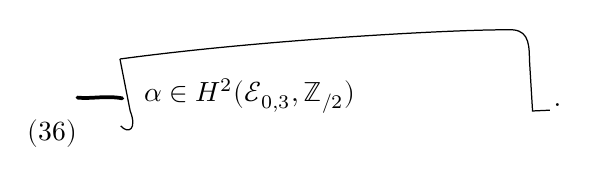
\begin{tikzpicture}[x=1cm,y=1cm,baseline=(formule.base)]
\node[anchor=west,inner sep=0pt] (formule) at (1.02,0)
  {$\alpha\in H^2(\mathcal E_{0,3},\mathbb Z_{/2})$};
\node[anchor=east,inner sep=0pt] at (0.18,-0.48) {$(36)$};
\draw[line width=0.45pt]
  (0.72,0.47) .. controls (2.65,0.73) and (5.13,0.85) .. (5.64,0.84)
  .. controls (5.89,0.86) and (5.92,0.70) .. (5.92,0.47)
  -- (5.96,-0.19) -- (6.18,-0.18);
\draw[line width=0.45pt]
  (0.72,0.47) -- (0.85,-0.19)
  .. controls (0.94,-0.42) and (0.83,-0.49) .. (0.73,-0.38);
\draw[line width=1.35pt,line cap=round]
  (0.18,-0.02) .. controls (0.35,-0.04) and (0.55,0.01) .. (0.75,-0.03);
\node[anchor=west,inner sep=0pt] at (6.22,-0.12) {.};
\end{tikzpicture}}
--- et rien ne dit que cette classe de cohomologie puisse s'effacer, en passant à un ss-groupe ouvert de $\mathcal E_{0,3}$.
\figure{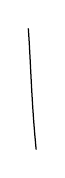
\begin{tikzpicture}[x=1cm,y=1cm]
\draw[line width=0.45pt]
  (0,1.05) .. controls (0.03,0.64) and (0.04,0.11) .. (0.10,-0.49);
\end{tikzpicture}}

\scanpage{526}

Mais en termes géométriques, \deleted{\unsure{bientôt}} les courbes elliptiques relatives \unsure{cherchées} sur \unsure{$U_{0,2}$|$U_{0,3}$} forment \unsure{\deleted{les}|les} sections d'un champ sur $(U_{0,3})_{\mathrm{et}}$, qui est une \deleted{\unsure{$\{\pm1\}$}}\inserted{$\mathbb Z_{/2}$}-gerbe --- l'obstruction se trouve donc dans un groupe de Brauer
\[
\beta\in H^2(U_{0,3},\mathbb Z_{/2}), \tag{37}
\]
or comme $U=U_{0,3}$ est une courbe alg. \deleted{\illegible{1}} affine sur un corps (il \unsure{suffirait} qu'elle ne soit de type $0,0$) \unsure{il s'ensuit} que l'hom canonique (à coefficients de torsion quelconques)
\[
H^*(\mathcal E_U,-)\longrightarrow H^*(U,-)
\]
est un iso. D'ailleurs, il \unsure{doit} être $\pm$ trivial que $\beta$ est l'image de $\alpha$ --- ce qui confirme l'\unsure{intuition|intention} que \deleted{\unsure{le}} si le relèvement est possible au niveau des groupes fondamentaux profinis (\unsure{arithmético-géométriques|arithmético-géométrique}) il l'est aussi au niveau des \unsure{multiplicités} modulaires elles-$\overline{\mathrm m}$, donc qu'on a une existence d'une courbe elliptique relative sur $U_{0,3}$ qui\ldots

\scanpage{527}
\mspage{269}

Il est \unsure{vrai} qu'il est bien \unsure{connu} qu'une classe de cohomologie (37) à coeff de torsion s'efface, en \unsure{passant} à une extension finie du \deleted{\unsure{$\mathbb Q$}} corps de base ($\mathbb Q$ en l'occurrence). En fait, on a une suite spectrale
\[
(38)\qquad H^*(U_{0,3},\mathbb Z_{/2})
\Longleftarrow E_2^{pq}
=H^p(\deleted{\unsure{\overline U_{0,3}}}\unsure{\mathbb Q},H^q(\overline U_{0,3},\mathbb Z_{/2}\unsure{)|))}
\]
et ici $H^q(\overline U_{0,3})=0$ pour $q\geq 2$, donc on trouve une suite exacte
\[
\deleted{\unsure{H^1(\mathbb Q)}\longrightarrow
\unsure{H^1(U_{0,3},\mathbb Z_{/2})}\longrightarrow
\unsure{H^1(\overline U_{0,3},-)}}
\]
\diagram{\begin{tikzcd}[ampersand replacement=\&,column sep=small]
\cdots \& E_2^{0,1} \arrow[r] \arrow[d,equal]
\& E_2^{2,0} \arrow[r] \arrow[d,equal]
\& \deleted{\unsure{E}}H^2(U_{0,3}) \arrow[r]
\& E_2^{1,1} \arrow[r] \arrow[d,equal]
\& E_2^{3,0} \arrow[d,equal] \& \cdots \\
\& H^0(\mathbb Q,H^1(\overline U)
\& H^2(\mathbb Q,\mathbb Z_{/2})
\&
\& H^1(\mathbb Q,\underset{\substack{\wr\\\mathbb F_2^2}}{H^1(\overline U)})
\& H^3(\mathbb Q,\unsure{\mathbb Z_{/2}|\mathbb F_2}) \&
\end{tikzcd}}

Je me \unsure{rends} compte enfin que l'existence d'un \deleted{\illegible{1}} relèvement, -- i.e. de la courbe elliptique hypothétique sur $U_{0,3}$ -- est tout à fait triviale, il suffit de \unsure{la|le} définir par l'équation
\[
y=\sqrt{\unsure{x|\dot x}(x-1)(x-\lambda)}
\]
i.e.
\[
y^2-x(x-1)(x-\lambda)=F(x,y;\lambda]=0
\]
ce qui définit une courbe plane affine,
\scanpage{528}
\unsure{on passe|ou passer} en coordonnées projectives
\[
F(x,y,z;\lambda)=y^2z-x^3+(1+\lambda)x^2z-\lambda xz^2=0
\]
\deleted{\unsure{pour|puis}} Je ne vais pas approfondir la question ici\unsure{.} \unsure{dans} quelle mesure ce choix est ``naturel''.

\deleted{\unsure{Une fois}} \inserted{\unsure{Il}} donne en tous cas un \unsure{homomorphis-}\deleted{\unsure{me extérieur}} \unsure{tout} ce qu'il y a de précis
\[
(39)\qquad M_{0,4}^{!}=U_{0,3}\longrightarrow M_{1,1}
\]
d'où un \unsure{hom.|hom} d'extensions
\diagram{\begin{tikzcd}[ampersand replacement=\&,column sep=small,row sep=small]
\& \& \widehat{\mathcal T}_{0,4}^{!+} \arrow[d,phantom,"\wr" description]
\& \unsure{N_{0,4}^{!}|\mathcal N_{0,4}^{!}} \arrow[d,phantom,"\wr" description] \& \& \\
(40) \& 1 \arrow[r]
\& \widehat\Pi_{0,3} \arrow[r] \arrow[d]
\& \mathcal E_{0,3} \arrow[r] \arrow[d]
\& \Gamma \arrow[r] \arrow[d,equal] \& 1 \\
\& 1 \arrow[r]
\& \widehat{\mathcal T}_{11}^{+} \arrow[r] \arrow[d,phantom,"\wr" description]
\& \mathcal E_{11} \arrow[r] \arrow[d,equal]
\& \Gamma \arrow[r] \& 1 \\
\& \& \unsure{\mathrm{Sl}}(2,\mathbb Z)^{\wedge}
\& \unsure{N_{1,1}|\mathcal N_{1,1}}\deleted{\unsure{\simeq\mathrm{Sl}(2,\mathbb Z)^{\wedge}}} \& \&
\end{tikzcd}}
défini mod \unsure{autom.|autom} \unsure{intérieure} par \deleted{et} un élément de $\widehat{\mathcal T}_{11}^{+}\simeq\unsure{\mathrm{Sl}}(2,\mathbb Z)^{\wedge}$, et au niveau des groupes \unsure{discrets|discret}
\[
\deleted{(41)}\qquad \Pi_{0,3}\longrightarrow\mathcal T_{1,1}^{+}
\]
\deleted{\unsure{mais} il n'est plus tellement}
\inserted{et même}
\[
(42)\qquad \Pi_{0,3}\hookrightarrow
\overbrace{\operatorname{Ker}\left(
\underset{\substack{\Vert\\\unsure{\mathrm{Sl}}(2,\mathbb Z)}}{\mathcal T_{1,1}^{+}}
\longrightarrow
\underset{\substack{\Vert\\\unsure{\mathrm{Sl}}(2,\mathbb Z_{/2})}}{\unsure{\mathfrak S_3}}
\right)}^{\unsure{\Gamma_2}}
\]
(et itou pour les groupes profinis). Ici $\Pi_{0,3}$ est tel que le sous-groupe de congruence du \unsure{deuxième} \unsure{mb|niv.} \deleted{\unsure{$\Gamma$}} soit $\unsure{\Gamma_2}$, \unsure{soit|est} produit direct de \unsure{ce|le} \unsure{sous-groupe|sous-groupes} $\Pi_{0,3}$ et de
\scanpage{529}
\mspage{270}
son centre $\pm1$. (Mais en fait, il y a \unsure{exactement} quatre sous-groupes de $\Gamma_2$ qui \unsure{réalisent} cette décomposition. Pour ne pas faire \unsure{de|des} jaloux, on pourrait regarder l'intersection des quatre, qui est un sous-groupe $\Gamma_2$ d'indice un diviseur de $2^4=16$ c'est l'intersection des noyaux \unsure{de|des} quatre homomorphismes $\Gamma_2\longrightarrow\deleted{\mathbb Z_{/2}}\ \unsure{\mathrm{Centre}}(\Gamma_2)=\{\pm1\}$,
\margin{\uline{NB} \unsure{Ça} doit être le noyau de $\mathrm{Sl}(2,\mathbb Z)^{\unsure{\wedge|*}}\longrightarrow\mathrm{Sl}(2,\mathbb Z/4\mathbb Z)$}
En tant que sous-groupe de $\Pi_{0,3}$, il est d'indice un diviseur de $8$ -- Ça m'étonnerait pas que ce soit juste le groupe des commutateurs de $\Pi_{0,3}$,) qui est d'indice $4$ -- il y a là toute une \unsure{situation} à élucider\ldots\,.
\margin{c'est vrai et c'est \unsure{$\simeq$|$\overline{\mathrm m}$} trivial\ldots}
\margin{Il n'est pas clair \deleted{si $\Pi_{0,3}$} est invariant en \unsure{tant} que ss-groupe de \deleted{\unsure{$\mathfrak S$}} $\mathcal T_{1,1}^{+}\simeq\mathrm{Sl}(2,\mathbb Z)$, i.e. stable par l'action ext. de $\unsure{\mathfrak S}_3$ sur $\mathrm{Sl}(2,\mathbb Z)$ -- je présume que oui, puisque $\unsure{\mathfrak S}_3$ opère aussi extérieurement sur $\Pi_{0,3}$ a priori\ldots\ $\mathcal T_{11}^{+}/\Pi_{0,3}$ serait une extension centrale \unsure{intéressante} de $\unsure{\mathfrak S}_3$ par $\{\pm1\}$\ldots}

Bien entendu, il faudrait aussi expliciter l'homomorphisme (42) (défini \unsure{mod} \unsure{autom.} intérieurs) par ses valeurs sur les générateurs $\unsure{l_0,l_1,l_2}$ -- j'y reviendrai peut-être tantôt.

\scanpage{530}

\uline{Théorème} L'action extérieure naturelle de $\Gamma_Q$ sur $\widehat{\mathcal T}_{1,1}^{+}$, et même sur $\widehat{\mathcal T}_{1,1}^{+\prime}=\widehat{\mathcal T}_{1,1}/(\pm1)$, est fidèle.
\figure{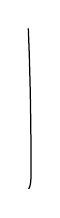
\begin{tikzpicture}[x=1cm,y=1cm]
\draw[line width=0.45pt]
  (0,1.05) .. controls (0.025,0.44) and (0.035,-0.19) .. (0.035,-0.78)
  .. controls (0.035,-0.91) and (0.025,-0.96) .. (0.005,-0.99);
\end{tikzpicture}}

On utilise le fait qu'on a un hom. ext. injectif
\[
\widehat{\Pi}_{0,3}\hookrightarrow\widehat{\mathcal T}_{1,1}^{\prime+}
\]
compatible avec l'action de $\Gamma$, en procédant comme pour la proposition du début (où $\widehat{\Pi}_{0,3}'$ jouait le rôle de $\widehat{\mathcal T}_{1,1}^{\prime+}$).

\uline{Corollaire} Les homomorphismes canoniques (surjectifs)
\[
\tag{43}
\Gamma_Q\longrightarrow\Gamma_{1,\nu}\qquad(\nu\geq1)
\]
sont injectifs, donc des isomorphismes.

Il suffit de le prouver pour $\Gamma_Q\longrightarrow\Gamma_{1,1}$ (puisque $\Gamma_{1,1}$ est un quotient de $\Gamma_{1,\nu}$, $\nu\geq1\ldots$), or on a un hom \unsure{\deleted{\illegible{1}}} $\Gamma_{1,1}\longrightarrow\mathrm{Aut\ ext}\,\widehat{\mathcal T}_{1,1}^{+}$ et on peut considérer le \unsure{composé}
\scanpage{531}
\mspage{271}

\[
\Gamma_{\mathbb Q}\unsure{-|\longrightarrow}\Gamma_{1,1}
\longrightarrow \operatorname{Aut\,ext}\widehat{\mathcal T}_{1,1}^{+}
\longrightarrow \operatorname{Aut\,ext}\widehat{\mathcal T}_{1,1}^{+'},
\]
par le théorème précédent ce composé est injectif, donc aussi
$\Gamma_{\mathbb Q}\longrightarrow\Gamma_{1,1}$, cqfd.

\uline{Remarque} On a vraiment l'impression, avec la proposition du début, et
le résultat précédent baptisé ``théorème'', d'avoir démontré deux fois
la $\overline{\mathrm m}$ chose, et avec la $\overline{\mathrm m}$ démonstration
encore ! Donc il est temps, après ce détour, de s'assurer qu'il en est
bien ainsi, i.e. que l'hom
$\widehat{\Pi}_{0,3}\longrightarrow\deleted{\unsure{\Pi}}\widehat{\mathcal T}_{1,1}^{+'}$ qu'on vient d'utiliser
s'identifie bel et bien à l'hom.
$\widehat{\Pi}_{0,3}\longrightarrow\widehat{\Pi}'_{0,3}$,
moyennant un iso. convenable (qui reste à décrire),
commutant aux actions extérieures de $\Gamma$,
qu'on se proposait de construire (cf (10) à (20)) --- et on l'a
perdu en route, en

\scanpage{532}

essayant de \deleted{\unsure{prouver}}\inserted{\unsure{trouver}}
$\Pi'_{0,3}\xrightarrow{\sim}\mathcal T_{1,1}^{+'}$ par
factorisation dans l'hom composé
\[
\Pi_{0,3}\xrightarrow{\substack{\mathrm{can.}\\\unsure{\mathrm{surj}}}}
\Pi'_{0,3}\longrightarrow\mathcal T_{1,1}^{+'}
\]
--- et on s'est en un sens fourvoyé, car l'hom ``naturel''
$\unsure{\varphi|\rho}\,\Pi_{0,3}\longrightarrow\mathcal T_{1,1}^{+'}$
sur lequel on est tombé n'était \uline{pas} \inserted{du tout} celui qu'on avait
en vue : j'étais à côté de mes pompes. Donc il me faut revenir à la charge !

\scanpage{533}
\mspage{272}

\uline{37} Théorie des Modules des courbes elliptiques via Legendre
(rigidification d'échelon 2). \unsure{)}

Je me rends compte que j'ai pas mal compliqué des choses pourtant bien
simples, au \S\ précédent. D'abord un remords de topologie des surfaces :

\uline{Proposition} \unsure{Soient|Soit}\deleted{\illegible{1}}
$X$ une surface topologique\unsure{${}^{*}$} paracompacte,
$G$ un groupe discret opérant proprement sur $X$, on suppose que pour tout
$x\in X$, le stabilisateur $G_x$ opère fidèlement sur un voisinage de $x$
(de sorte que $G$ opère fidèlement --- en fait les deux doivent être
équivalents) en préservant l'orientation locale (donc $G_x$ est
un groupe cyclique), de sorte que $Y=X/G$ est une surface top. paracompacte.
Considérons l'ens
\[
X^{!}=\{x\in X\mid G_x\ne(1)\}
\]
--- qui est une partie discrète de $X$ stable sous $G$ --- et l'image
$Y^{!}\unsure{\subset|\in}Y$ de $X^{!}$ --- partie discrète de $Y$ --- et
la ``signature'' sur $(Y,Y^{!})$, pour laquelle le coeff $d_y$ $(y\in Y^{!})$
est l'indice de ramification $\operatorname{ord}G_x$ en les
$x\in X$ au dessus de $y$. Pour tout $G$-revêtement $X'$ de $X$, considérons
alors $X'/G=Y'$ comme espace au dessus de $Y$. Alors :

\margin{\uline{Variante} $\mathcal G$ opère
\deleted{$X$ \illegible{2} $\mathcal G$}
\deleted{\unsure{opère}}\inserted{sur} $X$, \unsure{avec|son} sous-groupe
\uline{invariant} $G$ dans $\mathcal G$
satisfaisant les conditions ci-contre. On a alors, posant
\deleted{\illegible{1}} $Y=X/G$ avec \unsure{opér.} de
$\mathcal G/G=\mathcal H$
dessus :
\[
\deleted{\illegible{1}}\underline{\operatorname{Rev}}.
(X,\mathcal G)\unsure{\approxeq|\simeq}
\underline{\operatorname{Rev}}((Y,\underline d),\mathcal H),
\]
donc
\[
\Pi_1(X,\mathcal G,x)
\xrightarrow{\sim}
\Pi_1((Y,\underline d,\mathcal H),y).
\]
Application
\[
\mathfrak S_{0,3}\simeq
\mathcal T'_{1,1}
(\simeq\unsure{\mathrm{Gl}|\mathrm{Sl}}(2,\mathbb Z)/\pm1)
\]
ext de $\mathcal T_{0,3}=\mathfrak S_3
\times\mathbb Z/2$ par $\Pi_{03}$}
\scanpage{534}

a) $Y'$ est \deleted{un} \inserted{une surface top.,} rev. ramifié de $Y$, subordonné à la signature $\underline d\,\deleted{\illegible{1}}=\underline d(X/Y)$.

b) Le foncteur $X'\longmapsto Y'=X'/G$ est une équivalence de catégories
\[
(1)\qquad \mathrm{Rev}(X,G)\overset{\approx}{\longrightarrow}\mathrm{Rev}_{\underline d}(Y)
\]

\uline{NB} On peut expliciter un foncteur quasi-inverse, en associant à tout rev. ramifié $Y'$ de $Y$ compatible avec $\underline d$, \deleted{\illegible{2}} \inserted{le} $(X,G)$-revêtement ``normalisé'' (en un sens topologique facile à expliciter) de $X\times_Y Y'$. On a un énoncé analogue pour les schémas loc. noeth. réguliers de dim $1$, où le foncteur quasi-inverse s'obtient en normalisant $X\times_Y Y'$.

\uline{Corollaire} Soient $x\in X-X^{!}$, $y$ son image dans $Y$. On suppose $Y$ connexe (i.e. que $G$ opère transitivement sur l'ens des comp. connexes de $X$). Alors on a un isom canonique
\[
(2)\qquad \Pi_1(X,G;\unsure{a|x})\overset{\sim}{\longrightarrow}\Pi_1((Y,\underline d),y)
\]

\scanpage{535}
\mspage{273}

d'où, pour $X$ connexe, une suite exacte canonique
\[
(3)\qquad
1\longrightarrow
\deleted{\Pi_1((X,\unsure{G|1}),x)}\inserted{\Pi_1(X,x)}
\longrightarrow\Pi_1((Y,\underline d),y)\longrightarrow G\longrightarrow 1
\]

\uline{NB} On a \unsure{?} un corollaire analogue dans le contexte schématique, $X$ et $Y$ étant des schémas réguliers de dim $1$\unsure{.} --- ou, le cas échéant, des schémas relatifs lisses de dim rel. $1$ sur un $S$, mais dans ce cas il faudrait (si j'en ai besoin) faire un peu attention de préciser \unsure{l'énoncé|les énoncés} en forme raisonnable.

\uline{Exemple} Prenons $X=\mathbb P^1(\mathbb C)\setminus\{0,1,\infty\}=U_{0,3}(\mathbb C)$,
$G=\mathfrak S_3$ opérant de façon habituelle, donc (avec les \deleted{\unsure{notations}} \inserted{conventions} du \S\ précédent),
\deleted{$Y=\unsure{\mathbb P^1(\mathbb C)}\,\mathbb P^1(\mathbb C)$}
\inserted{identifiant} $\mathbb P^1(\mathbb C)/(G=\mathfrak S_3)$ à $\mathbb P^1_{\mathbb C}$, avec
\[
(4)\qquad
\begin{array}{rcll}
(0,1,\infty)&\longmapsto&0&d_0=2\\
(2,-1,\tfrac12)&\longmapsto&1&d_1=2\\
(j,\overline j)&\longmapsto&\infty&d_\infty=3
\end{array}
\]
on trouve $Y=\mathbb P^1(\mathbb C)\setminus\{0\}$, et $\underline d=2\{1\}+3\{\infty\}$.

On trouve donc un iso. can.
\[
(5)\qquad
\Pi^{1}((U_{0,3}(\mathbb C),\mathfrak S_3),x)
\simeq\Pi_1((\mathbb P^1(\mathbb C)\setminus\{0\},\underline d),\unsure{y})
\]

\scanpage{536}

\unsure{or|ou} malheureusement on ne peut prendre $x=P=j$, il faut prendre
$x\in\mathbb P^1(\mathbb C)\setminus\{0,1,\infty,2,-1,\tfrac12,j,\overline j\}$
--- le plus commode sera de prendre $x$ tel que $y=f(x)\,\unsure{\in|\leq|\leftarrow}$ soit le $\mathrm p^{\mathrm t}$-base \inserted{typique} $Q=j$ pour calculer le $\pi_1$ à ramification --- pour un tel $x$ on trouve donc un iso. canonique
\[
(5\,\mathrm{bis})\qquad
\Pi_1((U_{0,3}(\mathbb C),\mathfrak S_3),x)\simeq\Pi'_{0,3}
\]
et en choisissant une \inserted{$\mathfrak S_3$-}classe de chemins du point-base \inserted{initial} $P=j$ sur $\unsure{X_0|X}=U_{0,3}(\mathbb C)$ vers $x$, d'où un iso. corr. du premier mb de (5bis) \deleted{\illegible{1}} avec $\Pi_{0,3}$, on trouve un iso. can.
\[
(6)\qquad
\Pi_1((U_{0,3}(\mathbb C),\mathfrak S_3),P)\simeq\Pi'_{0,3}
\]
(qui change par autom. int. quand on modifie le choix d'une $\mathfrak S_3$-classe de chemins), d'où la suite exacte
\[
(7)\qquad
1\longrightarrow\Pi_{0,3}\longrightarrow\Pi'_{0,3}\longrightarrow\mathfrak S_3\longrightarrow 1,
\]
qui n'est autre que (9bis) du \S\ précédent, mais interprétée ici de façon bien plus transparente comme
\scanpage{537}
\mspage{274}

suite exacte d'homotopie pour $\mathfrak{S}_3$ opérant
sur $U_{0,3}(\mathbb{C})$. Et on trouve de $\overline{\mathrm m}$,
dans le cadre \unsure{arithméticogéométrique},
travaillant sur le schém. $U_{0,3}=U_{0,3\mathbb{Q}}$ et son
quotient $U_{0,3}/\mathfrak{S}_3\simeq\mathbb{P}^{1}_{\mathbb{Q}}\setminus\{0\}$, avec
la signature $2\{1\}+\unsure{3}\{\infty\}$ dessus, le
diagramme de suites exactes

\diagram{
\begin{tikzcd}[ampersand replacement=\&,column sep=large,row sep=large]
 \& 1 \arrow[d] \& 1 \arrow[d] \& \& \\
1 \arrow[r] \& \widehat{\Pi}_{0,3} \arrow[r] \arrow[d] \& \widehat{\Pi}'_{0,3} \arrow[r] \arrow[d] \& \mathfrak{S}_3 \arrow[r] \arrow[d,equal] \& 1 \\
1 \arrow[r] \& \mathcal{E}_{0,3} \arrow[r] \arrow[d] \& \mathcal{E}'_{0,3} \arrow[r] \arrow[d] \& \mathfrak{S}_3 \arrow[r] \& 1 \\
 \& \Gamma_{\mathbb{Q}} \arrow[r,equal] \arrow[d] \& \Gamma_{\mathbb{Q}} \arrow[d] \& \& \\
 \& 1 \& 1 \& \&
\end{tikzcd}
[(8) à gauche de la deuxième suite horizontale.
À gauche et un peu au-dessous de $\widehat{\Pi}_{0,3}$ :
$\widehat{\mathcal{T}}^{+}_{0,4}$, suivi de deux courts traits obliques parallèles
(signe $=$ qui l'égale à $\widehat{\Pi}_{0,3}$).
À gauche et un peu au-dessous de $\mathcal{E}_{0,3}$ :
$\unsure{N}^{!}_{0,4}$ (un court trait horizontal contre le ${}^{!}$), suivi de deux courts traits
obliques parallèles (signe $=$ vers $\mathcal{E}_{0,3}$).
À gauche et un peu au-dessous du premier $\Gamma_{\mathbb{Q}}$ :
$\Gamma_{0,4}$, suivi de deux courts traits obliques parallèles (signe $=$ vers $\Gamma_{\mathbb{Q}}$).]
}

Nous voulons maintenant mettre en
relation $U_{0,3}$, avec l'action de $\mathfrak{S}_3$
dessus, avec la multiplicité modulaire
$M_{11}$ pour les courbes elliptiques
(indices $\mathbb{Q}$ sous-entendus). C'est
domage d'ailleurs de travailler seulement sur $\mathbb{Q}$ --- je vais travailler
plutôt, sur $\mathbb{Z}[1/2]$ --- i.e. en car. \unsure{rés.|tj.} $\ne 2$.

\scanpage{538}

Au \S{} précédent j'ai identifié, un peu
vaseusement, $U_{0,3}=M^{!}_{0,4}$\unsure{,} à $M_{1,1}[2]'$\unsure{,}
(\deleted{dont}\inserted{sur lequel} $M_{1,1}[2]$
\deleted{\unsure{devrait être|devait être} \illegible{1}}\inserted{est une gerbe liée} par
$\mathbb{Z}/2$). Les ennuis techniques (plutôt,
les complications conceptuelles) tiennent
au fait que pour les courbes elliptiques
(plus gén, pour les variétés abéliennes de
dim quelconque), si $n$ est un entier $\ge 3$,
la "rigidification de Jacobi d'échelon $n$" est
bel et bien une rigidification (i.e.
tout autom d'une courbe elliptique
relative $E$ qui induit l'identité sur
${}_nE$ --- sous-schém. noyau de $n.\mathrm{id}_E$ --- est
l'identité --- mais il n'en est plus de
$\overline{\mathrm m}$ pour $n=2$, où $\unsure{u|n}$ est l'\uline{identité}\inserted{$\mathrm{id}_E$} \unsure{au} dessus
d'une partie ouverte fermée de $S$, et $-\mathrm{id}_E$
sur le complémentaire. Ceci suggère, pour
une meilleure compréhension, de coiffer
$M_{1,1}[2]$ par un $M_{1,1}(n)$, où $n$ est un
multiple de $2$ --- alors $M_{1,1}(n)$ dev. un
schém. ordinaire de t.f. sur $\operatorname{Spec}\mathbb{Z}$
(son image dans $\operatorname{Spec}\mathbb{Z}$ \unsure{sera|ser.} \inserted{l'ouvert} $\operatorname{Spec}\mathbb{Z}[1/n]$)
et au dessus de $\operatorname{Spec}[1/n]$, le \deleted{\unsure{schém.|schéma}}\inserted{topos modulaire}
\scanpage{539}
\mspage{275}

$M_{1,1}$ se récupère comme
\[
(9)\qquad
M_{1,1}\unsure{\simeq|\cong}
\bigl(M_{1,1}[n],\overbrace{\mathrm{Gl}(2,\mathbb Z/n\mathbb Z)}^{\Gamma_n}\bigr)
\]
(au dessus de $\operatorname{Spec}\mathbb Z[1/n]$)

\margin{attention, c'est bien $\mathrm{Gl}(2,\mathbb Z/n\mathbb Z)$, et \uuline{non} $\mathrm{Sl}(2,\mathbb Z/n\mathbb Z)$ qu'il faut prendre ici}

Ici $M_{1,1}[n]$ est le schém. qui représente le foncteur sur $(\mathrm{Sch})_{\unsure{\mathbb Z|S}}$
\[
S\longmapsto
\begin{gathered}
\text{ens des courbes elliptiques relatives}\\
\text{sur $S$, \uline{munies} d'un isom.}\\
(\mathbb Z/n\mathbb Z)^2_S\longrightarrow {}_nE
\end{gathered}
\]
\margin{ce foncteur \unsure{est|$\to$} représentable ssi $n\geq 3$ (donc il ne l'est pas pour $n=1,2$)}
sur lequel le groupe $\Gamma_n=\mathrm{Gl}(2,\mathbb Z/n\mathbb Z)=\operatorname{Aut}((\mathbb Z/n\mathbb Z)^2)$ opère de façon évidente. \deleted{La variété} Le \uline{schém. modulaire} (``grossier'', par opposition à la multiplicité ou topos modulaire) est décrit au dessus de $\mathbb Z/n\mathbb Z$ par
\[
(10)\qquad \widetilde M_{1,1}\simeq M_{1,1}[n]/\Gamma_n
\]
(au dessus de $\mathbb Z[1/n]$)

\uline{NB} Le schém. $\widetilde M_{1,1}$ \inserted{sur $\operatorname{Spec}\mathbb Z$} peut se décrire comme ``l'enveloppe représentable'' du foncteur non représentable
\[
S\longmapsto
\begin{gathered}
\text{classes d'\unsure{isom.|Isom.} des courbes}\\
\text{elliptiques relatives sur $S$ \ldots}
\end{gathered}
\]
-- itou sur un schém. de base (p.ex $\mathbb Q$, ou $\operatorname{Spec}\mathbb Z[1/n]$, quelconque \ldots

\scanpage{540}

Il faut faire attention qu'en tant que schém. sur $\mathbb Z[1/n]$ (ou sur $\mathbb Q$, en passant à la fibre \unsure{gén|gén.}) $M_{1,1}[n]$ \uline{n'est pas} relativement connexe (i.e. n'est pas à fibres géom. connexes). \unsure{En} effet, un iso.
\[
(\mathbb Z/n\mathbb Z)^2_S\simeq {}_nE
\]
implique, par passage à la puissance ext. $2^{\unsure{\mathrm{ième}|\mathrm{ème}}}$, un isom
\[
(\mathbb Z/n\mathbb Z)_S\xrightarrow{\sim}
\Lambda^2_{\mathbb Z/n\mathbb Z}\,{}_nE
\simeq \mu_n^{\otimes-1}(S)
\]
d'où un isom
\[
\mathbb Z/n\mathbb Z\simeq\mu_n(S)
\]
qui s'identifie (prenant \deleted{\unsure{et}} l'image de $1$ mod $n$) à une section de $\mu_n^*(S)$, où $\mu_n^*$ est le $(\mathbb Z/n\mathbb Z)^*$-torseur relatif sur $\operatorname{Spec}\mathbb Z[1/n]$ des ``racines primitives \unsure{$n$ièmes|$n$-ièmes} de $1$''. On a donc un morphisme canonique
\[
(11)\qquad M_{1,1}[n]\longrightarrow\mu_n^*
\]
et c'est ce morphisme qui est à fibres géom. connexes \inserted{\uuline{en car.0}}. Passant à la limite sur $n$ variable, on trouve \uline{sur $\mathbb Q$}
\[
(12)\qquad M_{1,1}[\infty]=\varprojlim_n M_{1,1}[n]
\longrightarrow\mu_\infty^*\overset{\inserted{\mathrm{iso.can}}}{\simeq}\operatorname{Spec}\Sigma
\]
\scanpage{541}
\mspage{276}

\unsure{(12)} où $\Sigma$ \inserted{$\subset\mathbb C$} est \unsure{la sous-extension} cyclotomique maximale de $\overline{\mathbb Q}_0$.

\deleted{\unsure{Le}} On récupère les $M_{1,1}[n']$, pour $n'\mid n$, \inserted{$n'\ne 1,2$,} à partir de $M_{1,1}[n]$ avec l'action de $\Gamma_n$ dessus, par
\[
(13)\qquad M_{1,1}[n']\simeq M_{1,1}[n]\wedge_{\Gamma_n}\Gamma_{n'}\simeq M_{1,1}[n]/K_{n,n'}
\]
\[
\text{sur }\operatorname{Spec}\mathbb Z[1/n]
\]
où
\[
(14)\qquad K_{nn'}=\operatorname{Ker}(\Gamma_n\longrightarrow\Gamma_{n'}).
\]

\margin{\uline{NB} $K_{n,n'}$ opère \uline{librement} sur le schéma $M_{1,1}[n]$ (si $n'\mid n$, $n'\ne 1,2$) --- mais pas bien sûr si $n'=1$ ou $2$.}

Si on applique cependant cette formule dans \unsure{le cas non licite|les cas non licites} $n'=1$ ou $2$, on trouve pour le cas $n'=1$, non $M_{1,1}$ mais $\widetilde M_{1,1}$ (schéma modulaire grossier), et pour $n'=2$, non $M_{1,1}[2]$ (qui n'est pas non plus un schéma) mais ce qu'on avait appelé au \S\ précédent $M_{1,1}[2]'$.

On peut \deleted{\unsure{déterminer|définir}} \inserted{expliciter} \inserted{$M_{1,1}$ et} $\widetilde M_{1,1}$ sur $\operatorname{Spec}\mathbb Z$ tout entier, \inserted{en termes des $M_{1,1}[n]$,} en les décrivant au \inserted{dessus des} deux ouverts $\operatorname{Spec}(\mathbb Z[1/n])$, $\operatorname{Spec}(\mathbb Z[1/n'])$ qui recouvrent $\operatorname{Spec}(\mathbb Z)$ (i.e. pour $(n,n')=1$) par (9) et (10), \inserted{(en y prenant d'abord $n$, puis $n'$)} et en ``recollant'' \deleted{dans} au dessus de $\operatorname{Spec}(\mathbb Z[\frac{1}{nn'}])$ par ces $\overline{\mathrm m}$s formules, appliquées à $nn'$\ldots

\scanpage{542}

On a d'ailleurs (pour mémoire)
\[
\text{\uline{Th}}\qquad \widetilde M_{1,1}\simeq\mathbb E^1_{\mathbb Z}\qquad(\text{sur }\operatorname{Spec}\mathbb Z)
\]

On peut épingler un tel isomorphisme (\unsure{défini|définit} à priori modulo le groupe affine entier $X\longmapsto\pm X+n$, $n\in\mathbb Z$) en \unsure{notant} qu'il y a dans $\widetilde M_{1,1}$ deux sections privilégiées sur $\mathbb Z$, dont les valeurs au pt générique correspondent aux deux classes d'isom des courbes elliptiques en car. $0$ (sur $\mathbb C$, p.ex) qui ont des autom. $\ne\mathrm{id},-\mathrm{id}$ --- les deux groupes \unsure{d'automs} qu'on obtient sont d'ailleurs $\mathbb Z/4\mathbb Z$ et $\mathbb Z/6\mathbb Z$ (très facile p.ex. par voie \unsure{transcend.te|transcendante}). Ce sont ce qu'on appelle sauf erreur les courbes elliptiques ``anharmoniques''. Sur un $M_{1,1}[n]$, le groupe des autom. rat.\,$/k$ d'une courbe elliptique décrite par un point $x$ de $M_{1,1}[n](k)$ s'identifie canoniquement au stabilisateur de $x$ dans $\Gamma_n$ :
\[
(15)\qquad\operatorname{Aut}(E_x)\simeq(\Gamma_n)_x
\]

\scanpage{543}
\mspage{277}

--- bien sûr, on a des énoncés idoines sur un schéma de base quelconque, pas néc. un corps. Cela montre déjà que les \unsure{automs} des courbes elliptiques sont liés de façon essentielle à la \uline{ramification} de $\Gamma_n$ opérant sur $\unsure{M_{1,1}[n]|M_{1,n}[n]}$. On trouve ainsi :

\uline{Proposition} (Sur $\operatorname{Spec}\mathbb Q$) Il y a exactement deux orbites de $\Gamma_n$ opérant sur $M_{1,1}[n]$ qui sont ``\deleted{singulières}\inserted{critiques}'', et qui correspondent à des stabilisateurs isomorphes resp. à $\mathbb Z/4\mathbb Z$ et $\mathbb Z/6\mathbb Z$, qui sont les groupes des \unsure{automs} des courbes elliptiques (``anharmoniques'') correspondantes.

\margin{$n\ne 1,2$}

On \unsure{notera|note} que $\Gamma_n$ \uline{n'opère pas} \unsure{fidèlt|fidèlement} sur $M_{1,1}[n]$ --- le noyau de cette opération est le s-groupe central $\{\pm1\}$, image du groupe correspondant de $\operatorname{Gl}(2,\mathbb Z)$ --- il correspond au groupe des automorphismes ``universels'' $\pm\mathrm{id}_E$ des courbes elliptiques $E$. Le groupe quotient
\[
(16)\qquad \Gamma'_n=\Gamma_n/\{\pm1\}
\]
\deleted{\unsure{(sur|sur}} opère \unsure{fidèlt|fidèlement}, et on peut regarder le ``topos mixte'' $(M_{1,1}[n],\Gamma'_n)$ --- on trouve

\scanpage{544}
aussitôt qu'il ne \uline{dépend pas} (à \unsure{équi.|équiv.} can. près) \uline{du choix de} $n$ [à cela près que l'ouvert de $\operatorname{Spec}\mathbb Z$ sur lequel ``il a un sens'' dépend de $n$\dots] -- et. en fait, on a :

\margin{donc à \unsure{condition} de se placer au dessus d'un schéma de base (tel $\operatorname{Spec}\mathbb Z[\frac{1}{nn'}]$) où $n,n'$ sont \unsure{tous} deux inversibles\dots}

\[
(17)\qquad (M_{1,1}[n],\Gamma'_n)\simeq M_{1,1}'
\]
\[
(\text{au dessus de }\operatorname{Spec}\mathbb Z[1/n])
\]
où la \deleted{topos} \inserted{multiplicité schématique} modulaire $M_{1,1}'$ est \unsure{décrite|décrit}, en termes des courbes elliptiques ``\unsure{définies} mod symétrie'', comme au \S\ précédent.

\uline{Remarque.} La proposition précédente semble dépendre de $n$ -- mais on voit a priori \deleted{que} (grâce au fait que les $\Gamma_{n,n'}$ \inserted{($n'\mid n$, $n'\ne1,2$)} (\unsure{opérant|opèrent} librement) que si elle est valable pour \uline{un} $n$, elle est valable pour tous.

\deleted{\unsure{Cor.}} Notons \deleted{que} aussi

\uline{Corollaire de la proposition.} \inserted{(car. 0)} Les stabilisateurs \uline{dans $\Gamma'_n$} (le groupe qui opère \uline{\unsure{fidèlement}} sur $M_{1,1}[n]$) des points des \unsure{deux} orbites critiques sont resp. $\mathbb Z/2\mathbb Z$ et $\mathbb Z/3\mathbb Z$. \deleted{\illegible{1}}

\margin{valable pour $n\unsure{\ne|=|\geq}2$, \unsure{cf|cf.} plus bas}

\scanpage{545}
\mspage{278}
On a supposé ici que $n\ne1,2$ -- mais rien ne nous empêche de regarder aussi \inserted{sur}
\[
(18)\qquad M_{1,1}[2]'\overset{\mathrm{dfn}}{=}M_{1,1}[2m]/\Gamma_{2m,2}
=M_{1,1}[2m]/\unsure{\Gamma_{2m,2}|\Gamma'_{2m,2}}
\]
(où $m$ est un entier quelconque, $\ge2$)
l'action de $\Gamma_2\simeq\operatorname{Gl}(2,\mathbb Z/2\mathbb Z)\simeq\operatorname{Sl}(2,\mathbb Z/2\mathbb Z)\simeq\unsure{\mathfrak S_3|\mathcal S_3}\simeq\Gamma_{2m}/\Gamma_{2m,2}$. \deleted{\unsure{Alors qu'|Alors que}} Il n'est plus vrai, \inserted{certes,} que $\Gamma_{2m,2}$ opère \unsure{librement} sur $M_{1,1}[2m]$ -- car $\Gamma_{2m,2}$ contient l'élément $-1\in\Gamma_{2m}$ correspondant à la symétrie universelle $-\operatorname{id}_E$ -- i.e. \inserted{\unsure{à}} l'élément \deleted{\unsure{de}} $-1$ de $\operatorname{Gl}(2,\mathbb Z)$. Mais le résultat général de rigidité rappelé au début implique que \deleted{$\Gamma'_{2m,2}=\Gamma_{2m,2}/\pm1$}
\[
(19)\qquad\Gamma'_{2m,2}\overset{\mathrm{dfn}}{=}\Gamma_{2m,2}'/\pm1
\simeq\operatorname{Ker}(\Gamma'_{2m}\longrightarrow\Gamma'_2\simeq\unsure{\mathfrak S_3|\mathcal S_3})
\]
opère \deleted{\unsure{fi}} \inserted{encore} \uline{librement} sur $M_{1,1}[2m]$ -- et cela implique que le cor. de la prop. est valable encore pour l'action de $\Gamma'_2\,(\xleftarrow{\sim}\Gamma_2\simeq\unsure{\mathfrak S_3|\mathcal S_3})$ sur $M_{1,1}[2]'$.

\uline{Digression terminologique.} $M_{1,1}$ \inserted{${}=M_{1,1}[1]$} et les

\scanpage{546}
\mspage{278}
\figure{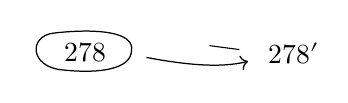
\begin{tikzpicture}[x=1cm,y=1cm,baseline=(ancien.base)]
\node[inner sep=0pt] (ancien) at (0,0) {$278$};
\draw[line width=0.45pt]
  (0.58,0.02) .. controls (0.63,0.27) and (0.13,0.31) .. (-0.40,0.25)
  .. controls (-0.73,0.22) and (-0.72,-0.19) .. (-0.28,-0.22)
  .. controls (0.20,-0.27) and (0.57,-0.20) .. (0.58,0.02);
\draw[->,line width=0.45pt]
  (0.77,-0.06) .. controls (1.25,-0.15) and (1.70,-0.20) .. (2.06,-0.11);
\draw[line width=0.4pt] (1.57,0.09) -- (1.95,0.04);
\node[anchor=west,inner sep=0pt] at (2.31,-0.015) {$278'$};
\end{tikzpicture}}
\mspage{278'}
$M_{1,1}[n]$ ($n\in\mathbb N^*$) sont \unsure{définis} \unsure{a|à} priori comme des \uline{multiplicités} schématiques modulaires, i.e. a) comme des topos loc. annelés loc. isom. au topos étale d'un schéma (en l'occurrence, de type fini sur $\operatorname{Spec}\mathbb Z$, ou sur $\mathbb Q$ si on travaille en car. 0) et b) \unsure{définis}, à équivalence près définie elle-$\overline{\mathrm m}$ à \unsure{isom|isom.} unique près, comme ``représentant'' les \deleted{\illegible{1}} ``foncteurs'' correspondants
\[
S\longmapsto
\begin{gathered}
\text{catégorie des courbes elliptiques}\\
\text{relatives sur }S\text{, avec rigidification}\\
\text{de Jacobi d'échelon }n\text{ i.e.}\\
\text{iso.}\quad(\mathbb Z/n\mathbb Z)_S\simeq{}_nE\\
={}\unsure{\mathcal{E}ll_n}(S)
\end{gathered}
\]
donc par construction on a \inserted{pour tt schéma $S$} une équivalence
\[
\unsure{\mathcal{E}ll_n}(S)\unsure{\simeq|\cong}
\text{\uline{$\operatorname{Hom}$}}_{\substack{\text{topos loc.}\\\text{annelés}\\\text{i.e. hom de}\\\text{multiplicités}}}
(S,M_{1,1}[n])
\]
Pour que les catégories $\unsure{\mathcal{E}ll_n}(S)$ soient \uline{discrètes}, \deleted{\illegible{1}} ou encore $M_{1,1}[n]$ soit un schéma, ou encore que les autom. d'une

\scanpage{547}
\mspage{279}

courbe ell. \unsure{respectant|respectent} une rigid. de Jacobi d'échelon $n$ \unsure{soient} l'identité, il \unsure{f et s.} que $n\geq 3$ i.e. $n\neq 1,2$. Donc $M_{1,1}[2]$ n'\uline{est pas} un schéma -- mais $M'_{1,1}[2]$ en est un, et $M_{1,1}[2]\to M_{1,1}[2]'$ est un \deleted{\illegible{1}} isom local (décrit entièrement par une $\mathbb Z/2\mathbb Z$-gerbe sur $M_{1,1}[2]'$). \deleted{\unsure{On considère bien sûr}} \inserted{\unsure{Il} faut quand $\overline{\mathrm m}$ prendre la} peine de définir
\diagram{\[
\tag{20}
\begin{tikzcd}[ampersand replacement=\&,column sep=large,row sep=large]
M_{1,1}[2] \arrow[r] \arrow[d,phantom,"{\simeq}"{description,rotate=90},"{\text{``théor.''}}"{description,xshift=3em}] \& M_{1,1}[2]' \arrow[d,phantom,"{\simeq}"{description,rotate=90},"{\text{``dfn''}}"{description,xshift=3em}] \\
(M_{1,1}[2m],\Gamma_{2m,2}) \& M_{1,1}[2m]/\Gamma'_{2m,2} \arrow[d,phantom,"{\Vert}"{description}] \\
\& M_{1,1}\unsure{(2m)|[2m]}/\Gamma_{2m,2}
\end{tikzcd}
\]}
comme l'homomorphisme canonique du ``passage au quotient grossier'' -- qui a un sens chaque fois qu'un groupe discret (disons)\unsure{\S} $G$ opère sur un schéma (disons) $X$, comme un morphisme
\[
\tag{21}
(X,G)\longrightarrow X/G=Y
\]
dont le foncteur \unsure{image} inverse (faisceaux sur $Y=X/G\longrightarrow G$-faisceaux sur $X$) est évident. Ici on a un sous-groupe inv. \unsure{$\mathfrak z$|$z$} de $G$ qui opère \unsure{trivialt|trivialement} sur $X$, tel que $G/\unsure{\mathfrak z|z}$ opère librement, ce qui signifie que le morphisme

\scanpage{548}

(21) se factorise en
\[
\tag{22}
(X,G)\longrightarrow
\left(X,\underbrace{G/\unsure{\mathfrak z|z}}_{G'}\right)
\overset{\sim}{\longrightarrow}Y=X/G=X/G',
\]
de sorte que le morphisme de multiplicités (21) s'identifie aussi, simplement, à
\diagram{\[
\tag{23}
\begin{tikzcd}[ampersand replacement=\&,column sep=large,row sep=large]
(M_{1,1}[2m],\Gamma_{2m,2}) \arrow[r] \& (M_{1,1}[2m],\Gamma'_{2m,2}) \arrow[d,phantom,"{\simeq}"{description,rotate=90}] \\
\& M_{1,1}[2]'
\end{tikzcd}
\]}

Par contre, si on veut descendre jusqu'à $M_{1,1}[1]'=M_{1,1}'$, en passant au quotient (au sens ``grossier'') de $M_{1,1}[n]$ par $\Gamma'_n$, le morphisme
\diagram{\[
\tag{24}
\begin{tikzcd}[ampersand replacement=\&,column sep=large,row sep=large]
(M_{1,1}[n],\Gamma'_n) \arrow[r] \arrow[d,phantom,"{\Vert}"{description}] \& M_{1,1}[n]/\Gamma'_n \arrow[d,phantom,"{\Vert}"{description}] \\
M_{1,1}' \& \widetilde M_{1,1}
\end{tikzcd}
\]}
n'est plus un ``iso'' i.e. n'est plus une équivalence, car $\Gamma'_n$ n'opère pas librement -- il a \inserted{($\overline{\mathrm m}$ en car. $0$)} de la ramification de degré $2,3$.

[Si cependant on exclut les courbes elliptiques anharmoniques, \unsure{sa|ça} marcherait -- ce n'est ``qu'au voisinage'' de ces courbes elliptiques que (24) n'est pas un iso\ldots

\scanpage{549}
\mspage{280}

En fait, les raisonnements du \S{} précédent établissent un isomorphisme (\unsure{valable} sur \inserted{le} $\mathrm{Spec}\,\unsure{\mathbb Z[1/n]}$ de $\mathbb Z[1/2]$)
\[
(25)\qquad M_{1,1}[2]'\simeq M_{0,4}^{!}\simeq U_{0,3}
\]
(\unsure{valable} sur $\mathrm{Spec}\,\mathbb Z[1/2]$)

\margin{NB \unsure{l'image} de $M_{1,1}[2]'$ dans $\mathrm{Spec}\,\mathbb Z$ est $\mathrm{Spec}\,\mathbb Z[1/\unsure{n|2}]$, tandis que celle de $M_{0,4}^{!}\simeq U_{0,3}$ est $\mathrm{Spec}\,\mathbb Z$ \unsure{tt} entier}

et cet isomorphisme est compatible avec les opérations de \deleted{$\unsure{\Gamma'_2\simeq\Gamma}$}
\[
(26)\qquad \Gamma'_2\simeq\Gamma_2=\operatorname{Gl}(2,\mathbb Z/2\mathbb Z)=\operatorname{Sl}(2,\mathbb Z/2\mathbb Z)
\]
sur $M_{1,1}[2]'$ d'une part, de $\unsure{\mathfrak S_3|\mathcal S_3}$ sur $U_{0,3}$ d'autre \unsure{part|parts}, quand on considère l'isomorphisme
\[
(27)\qquad
\begin{array}{ccc}
\Gamma_2 & \xrightarrow{\sim} & \unsure{\mathfrak S_3|\mathcal S_3}\\
\Vert &&\\[-4pt]
\operatorname{Gl}(2,\mathbb F_2)&&
\end{array}
\]
qui associe, à tout autom de $\mathbb F_2^2$, son action sur les trois éléments non nuls, $\underline{\alpha}=(1,0)$, \inserted{$\underline{\beta}=$}$(0,1)$, et $\underline{\gamma}=(1,1)=\underline{\alpha}+\underline{\beta}$ (de sorte qu'on a d'ailleurs) \deleted{\illegible{2}}
\[
(28)\qquad \gamma=\alpha\unsure{+|-}\beta,\quad \unsure{\alpha|\beta}=\beta\unsure{+|-}\gamma,\quad \beta=\unsure{\gamma}+\alpha.
\]
Il faudrait expliciter cette compatibilité, en \unsure{considérant} l'action naturelle de $\unsure{\mathfrak S_4|\mathcal S_4}$ sur $M_{0,4}^{!}$, $M_{0,n}^{!}$ étant la multiplicité modulaire définie par

\scanpage{550}

\[
(29)\qquad
\underline{\operatorname{Hom}}_{\text{multiplicités}}(S,M_{0,n}^{!})\simeq
\begin{gathered}
\text{catégorie des}\\
\text{\unsure{courbes|droites} relatives}\\
\text{sur }S,\ \text{loc. isom. à }\mathbb P^1_S\\
\text{(pour top. étale) et munies}\\
\text{de }n\text{ sections mutuellement}\\
\text{\unsure{disjointes} \unsure{numérotées}}\\
\deleted{\illegible{1}}\quad\unsure{s_1|s_0},s_2,\ldots s_n
\end{gathered}
\]

\margin{Si on veut une représentabilité pour $n=0,1,2$, il ne suffit plus de travailler avec \unsure{la topologie étale|les topologies étales} --- il faut des top. fppf p.ex...}

\uline{NB} c'est représentable bel et bien par une multiplicité ssi $n\geq3$, \inserted{i.e. si le champ \unsure{en|des} groupoïdes qu'on veut \unsure{représenter} est ``rigide'' ---} et alors la multiplicité est $\overline{\mathrm m}$ un schéma, isomorphe d'ailleurs \unsure{canonique|canoniquement} au \inserted{\unsure{ss-}}schéma
\[
\underline{\operatorname{Mon}}(I_{n-3},U_{0,3})\subset U_{0,3}^{I_{n-3}},
\]
où ici
\[
I_{n-3}=\{i\in\mathbb N\quad3<i\leq n\deleted{\unsure{-3}}\}
\]
--- ainsi \deleted{\illegible{1}}
\[
M_{0,3}^{!}\xrightarrow{\sim}\mathrm{Spec}\,\mathbb Z\quad\text{(schéma final)},\quad\text{et}
\]
\[
M_{0,4}^{!}\xrightarrow{\sim}U_{0,3}=\mathbb P^1_{\mathbb Z}\setminus\{\text{sections \deleted{\illegible{1}} }0,1,\infty\}=\mathrm{Spec}\,\mathbb Z[T]\Bigl[\frac{1}{T(T-1)}
\]

Mais on fera attention qu'il y a une opération naturelle de $\unsure{\mathfrak S_n|\mathcal S_n}$ sur $M_{0,n}^{!}$, donc sur $\underline{\operatorname{Mon}}(I_{n-3},U_{0,3})$ --- \deleted{\unsure{dont|donc}} alors que l'on ne voit a priori que l'action de $\unsure{\mathfrak S_3|\mathcal S_3}\times\unsure{\mathfrak S_{n-3}|\mathcal S_{n-3}}$ sur ce dernier: l'isom canonique
\[
(30)\qquad M_{0,n}^{!}\simeq\unsure{\operatorname{Mon}}(I_{n-3},U_{0,3})\subset U_{0,3}^{I_{n-3}}
\]
\[
\text{(où }I_{n-3}=\{i\in\mathbb N\mid\deleted{\unsure{2}}3<i\leq n\}\text{)}
\]
ne tient compte que des opérations naturelles \unsure{du|des}
\scanpage{551}
\mspage{\unsure{281}}

bijection canonique
\[
\tag{33}
\widetilde I \xrightarrow{\sim} V(I)^*
\overset{\mathrm{df}}{=} V(I)\setminus\{0\}
\]
en associant à une partition $I=I'\cup I''$, avec
$I',I''$ de cardinal $2$, la \inserted{seule} permutation
\unsure{\inserted{(paire)}|\deleted{\inserted{(paire)}}} de $I$
\deleted{formée de} qui \unsure{invarie} $I',I''$ et \unsure{induise|induit} sur
chacun \unsure{sa} permutation non triviale. (Les éléments
de $\mathfrak{S}_I$ obtenus ainsi sont aussi les \uline{permutations}
\uline{paires} \uline{d'ordre $2$}, \deleted{\unsure{)}} qui avec l'identité forment
donc le sous-groupe $V(I)$).

On trouve, si $i\in I$, d'où $I\setminus\{i\}$ de
cardinal $3$, \deleted{\unsure{que}} une application canonique
\[
\tag{34}
I\setminus\{i\}\longrightarrow\widetilde I
\]
en associant à $j\in I\setminus\{i\}$ la partition
de $I$ en $\{i,j\}$ et en son complémentaire.
Cette bijection étant compatible avec le
transport de \unsure{structures|structure}, on en conclut
que l'isom. correspondant
\[
\tag{35}
\mathfrak{S}_{I\setminus\{i\}}\simeq\mathfrak{S}_{\widetilde I}
\]
\deleted{\unsure{qui}} est \deleted{\unsure{compat}} aussi le composé
\[
\tag{36}
\underset{\substack{\text{stabilisateur de}\\ i\text{ dans }\mathfrak{S}_I}}
{\mathfrak{S}_{I\setminus\{i\}}}
\hookrightarrow\mathfrak{S}_I\longrightarrow\mathfrak{S}_{\widetilde I},
\]
donc les quatre sous-groupes symétriques
d'indice $3$ $\mathfrak{S}_{I\setminus\{i\}}$ de $\mathfrak{S}_I$ $(i\in I)$\unsure{.|,}

\scanpage{552}
sont canoniquement \unsure{isomorphes} à $\mathfrak{S}_{\widetilde I}$
--- donc entre eux, \deleted{\unsure{mais}} par des isom. qui
\deleted{\unsure{ne}} sont \deleted{\unsure{pas}} d'ailleurs \deleted{\illegible{1}} déduits des bijections
canoniques \deleted{\unsure{égales}}
\[
  (\deleted{\unsure{39}}\inserted{37})\qquad
  I\setminus\{i\}\xrightarrow{\sim}I\setminus\{j\}
  \qquad(i\ne j,\ i,j\in I)
\]
canoniques, égales à \deleted{l'identité}
\inserted{la \uline{transposition} (non à l'identité)} sur $I\setminus\{i,j\}$.
\inserted{Cette bijection en effet est le composé}
\deleted{(En effet, ces bijections \unsure{ne forment pas un}}
\[
  I\setminus\{i\}\xrightarrow{\sim}\widetilde I
  \xrightarrow{\sim}I\setminus\{j\}
  \qquad\text{---}
\]
\deleted{\unsure{syst.} transitif d'isom.)}
et pour $i,j$ variables, ces isom. forment un
syst. transitif d'isom.

Revenant à l'action de $\mathfrak{S}_4$ sur
$M_{\unsure{0},4}^{!}$, la clef de la \unsure{compréhension}
est donnée par ceci :

\uline{Proposition} Considérons le ss-groupe
$V(\deleted{\unsure{4}}\inserted{I})$ de $\mathfrak{S}_{\deleted{\unsure{4}}\inserted{I}}$ formé de $1$ et des involutions
paires. Alors l'action de $V(\deleted{\unsure{4}}\inserted{I})$ sur $M_{0,\deleted{\unsure{4}}\inserted{I}}^{!}$
est triviale, \unsure{\&|Si} donc \deleted{$V(I)$} $\mathfrak{S}_I$ agit
sur $M_{0,I}^{!}$ par l'intermédiaire de
$\mathfrak{S}_I/V(I)=\mathfrak{S}_{\widetilde I}$.
\figure{\begin{tikzpicture}[x=1cm,y=1cm]
\draw[line width=0.45pt]
  (0,3.45) .. controls (0.00,3.22) and (0.015,3.04) .. (0.045,2.90);
\draw[line width=0.45pt]
  (0.04,1.28) .. controls (0.055,0.83) and (0.055,0.35) .. (0.035,0.10)
  .. controls (0.03,0.04) and (0.015,0.015) .. (0,0);
\end{tikzpicture}}

\margin{\uline{NB} $M_{0,I}^{!}$ se définit en \unsure{termes} de $I$, pour tt ens\unsure{.} $I$ de card\unsure{.} $\geq 3$, comme $M_{0,n}^{!}$}

\uline{Corollaire} Soit $i\in I$, alors l'action
de $\mathfrak{S}_{I\setminus\{i\}}\subset\mathfrak{S}_I$ sur $M_{0,I}^{!}$ est déduite
de celle de $\mathfrak{S}_{\widetilde I}$ via l'isom can $\mathfrak{S}_{I\setminus\{i\}}\xrightarrow{\sim}\mathfrak{S}_{\widetilde I}$

\scanpage{553}
\mspage{28\unsure{0|1}bis}
\deleted{\unsure{de}} des ss-groupes
\[
 (31)\qquad \mathfrak{S}_3\times\mathfrak{S}_{n-3}\subset\mathfrak{S}_n
\]
de $\mathfrak{S}_n$ sur $M_{0,n}^{!}$, et pas de \unsure{celle|celles} de
$\mathfrak{S}_n$ tout entier. Dans le cas de $n=4$,
l'opération de $\Gamma'_2=\mathrm{Sl}(2,\mathbb{F}_2)\simeq\mathfrak{S}_3$ sur
$M_{0,4}^{!}$ qui nous intéresse, est celle qui
correspond au sous-groupe $\mathfrak{S}_{\unsure{1}}\times\mathfrak{S}_3\subset\mathfrak{S}_4$,
qui fixe le premier élément (\unsure{correspond.} à
la section nulle d'une courbe elliptique
--- \deleted{\unsure{qui}} et qui permute les trois \unsure{suivants}
\unsure{correspondts} aux trois éléments d'ordre $2$
d'une courbe ell. géom en \unsure{car.} $\ne 2$, qui
sont les trois autres \unsure{p\textsuperscript{t}} fixes de
$x\mapsto -x$, alors que l'opération \unsure{naïve|naive} de
$\mathfrak{S}_3$ sur $U_{0,3}$ correspond au ss-groupe
$\mathfrak{S}_3\times\mathfrak{S}_1$ de $\mathfrak{S}_4$, qui fixe les trois premiers
éléments. Petite question de gymnastique
\unsure{schématique} (\unsure{indépendante|indépendts} maintenant de la
géométrie des courbes elliptiques, mais
histoire de géom. projective de dim $1$) :
comment passer d'une de ces \deleted{\unsure{représentations}}\inserted{actions de}
$\mathfrak{S}_3$ à l'autre ? On a envie de prouver que
ce sont les $\overline{\mathrm m}$s !

\scanpage{554}
Notons que si $I$ est un ens. à $4$
éléments, alors il lui est associé un
ens. à trois éléments des ``partitions de
type $(2,2)$'' $P_{2,2}(I)=\widetilde I$, et l'hom
\[
 (32)\qquad
 \diagram{\begin{tikzcd}[ampersand replacement=\&, row sep=small,column sep=large]
 \mathfrak{S}_I \arrow[r] \arrow[d,phantom,"\simeq"{rotate=90}]
   \& \mathfrak{S}_{\widetilde I} \arrow[d,phantom,"\simeq"{rotate=90}] \\
 \mathfrak{S}_4 \& \mathfrak{S}_3
 \end{tikzcd}}
\]
est surjectif --- son noyau est un sous-groupe
isomorphe (\unsure{non} can.\textsuperscript{t}) à $\mathbb{F}_2\times\mathbb{F}_2$ --- donc un
groupe commutatif \inserted{$V(I)$} annulé par $2$, i.e. un
vectoriel sur $\mathbb{F}_2$, et en tt que tel de dim $2$.

En fait, $V(I)$ \unsure{opérant} sur $I$ fait de $I$
un $V(I)$ torseur --- donc $I$ est muni canoniquement
d'une structure \unsure{de|d'} \deleted{\unsure{espace}}\inserted{plan} affine sur $\mathbb{F}_2$,
et $V(I)\subset\mathfrak{S}_I$ est le groupe de ses
translations, $\mathfrak{S}_I$ \unsure{s'interprétant|s'interprète} comme le
groupe des autom. affines de $I$ (\uline{\unsure{tte}} permutation
de $I$ est affine --- il \deleted{\unsure{n'}} y a sur l'ens
$I$ $1$ et $1$ seule structure de plan affine sur
$\mathbb{F}_2$), et $\mathfrak{S}_{\widetilde I}$ comme le groupe $\mathrm{Aut}(V(I))$
--- ce qui suggère d'interpréter $\widetilde I$ comme
l'ens des trois éléments non nuls de $V(I)$, et
en effet, on constate que \deleted{\unsure{les}} l'on a une

\scanpage{555}
\mspage{282}

provenant de $I\setminus\{i\}\xrightarrow{\sim}\widetilde I$.

En particulier, pour $I=[1,2,3,4]$, pour
comparer l'action de $\mathfrak{S}_{\{1,2,3\}}$ et de
$\mathfrak{S}_{\{2,3,4\}}$ sur $M_{0,4}^{!}\simeq U_{0,3}$ --- où la première
est l'action standard de $\mathfrak{S}_3$ sur $U_{0,3}$,
la deuxième celle de $\mathfrak{S}_3$ sur $M_{1,1}[2]'$,
on utilise l'isom.
\[
\tag{38}
\mathfrak{S}_{\{1,2,3\}}\simeq\mathfrak{S}_{\{2,3,4\}}
\]
explicité dans (37), correspondant à la
bijection
\[
1\mapsto4,\quad 2\mapsto3,\quad 3\mapsto2
\]
des \unsure{ens.} d'indices, qui correspond donc
à l'\unsure{autom.}
\[
\tag{39}
\operatorname{int}(\sigma_1):\mathfrak{S}_3\longrightarrow\mathfrak{S}_3
\]
en identifiant maintenant les deux ens.
d'indices $[1,2,3]$, $[2,3,4]$ à $\{0,1,\infty\}$,
et en désignant par $\sigma_i\in\mathfrak{S}_{\{0,1,\infty\}}$
\inserted{(pour $i\in\{0,1,\infty\}$)} la
transposition des éléments $\ne i$. Donc

\uline{Corollaire} L'isom. canonique
\[
U_{0,3}\xrightarrow{\overset{\varphi}{\sim}}M_{1,1}[2]'
\qquad (\text{sur }\mathbb Z[1/2]),
\]
quand on fait opérer $\mathfrak{S}_3=\mathfrak{S}_{\{0,1,\infty\}}$ sur
l'un et l'autre membre, est compatible
avec ses opérations, \uline{via} l'\unsure{autom.} $\operatorname{int}(\unsure{\sigma_1|\sigma_i})$, i.e.

\scanpage{556}

\[
\tag{40}
\varphi(u.x)=(\unsure{\sigma_1|\sigma_i}\,u\,\unsure{\sigma_1^{-1}|\sigma_i^{-1}})\varphi(x)
\]

Il faut quand $\overline{\mathrm m}$ démontrer la prop. 4,
qui \unsure{équivaut} bien sûr à ceci

\uline{Corollaire} Soit $X$ une droite projective
relative sur \unsure{schém.} $S$, $I$ \unsure{ens} à quatre él.,
$(\deleted{\unsure{\sigma_i}}s_i)_{i\in I}$ une famille de sections \unsure{mutuellement|mutuellemt}
disjointes, et $\sigma$ une \deleted{\unsure{transposition}}\inserted{\unsure{involution}} paire de
$I$ (correspondant à une partition $I=\{i_1,i_2\}\cup\{i_3,i_4\}$
par $\sigma i_1=i_2$, $\sigma i_2=i_1$, $\sigma i_3=i_4$, $\sigma i_4=i_3$). Alors $\exists$
\unsure{autom.} (évidemment unique) $u$ de $X$,
tel que $u\circ s_i=s_{\sigma i}$.

\uline{Dém} OPS $X=\mathbb P^1_S$, $\unsure{s_1|s_{i_1}}=0$, $s_{i_2}=\infty$, donc
$\unsure{s_{i_2}|s_{i_4}},s_{i_3}$ s'identifient à des sections de
$\underline{\mathcal O}_S^*$, on prendra \deleted{\illegible{1}} $u$ défini par
\[
u(z)=\lambda/\unsure{z|Z}\qquad\lambda\in\Gamma(S,\mathcal O_S^*)
\]
qui échange $0$ et $\infty$, et la condition
pour échanger $s_2,s_3$ \unsure{ser.|s'écr.} $\lambda/s_3=s_4$, $\lambda/s_4=s_3$
i.e. $\lambda=s_3s_4$ (\uline{NB} il \unsure{suffisait|suffirait} que
$(s_1,s_2,s_3)$ et $(s_1,\unsure{s_2|s_1},s_4)$ \unsure{sont|soient} mutuellement disjointes ---
pas la peine que $s_3,s_4$ soient mutuellement
disjointes $\ldots$)

\scanpage{557}
\mspage{283}

Plaçons-nous à nouveau sur $\mathbb Q$ (pour fixer
les idées), et considérons les groupes fondamentaux
des multiplicités modulaires $M_{1,1}$, $M_{1,1}'$.
On part de
\[
\tag{41}
\left\{
\diagram{\begin{tikzcd}[ampersand replacement=\&, column sep=small,row sep=large]
M_{1,1}\arrow[d]\arrow[r,phantom,"\simeq" description]
  \& (M_{1,1}[n],\Gamma_n)\arrow[d]
  \& (n\geq3) \\
M_{1,1}'\arrow[r,phantom,"\simeq" description]
  \& (M_{1,1}[n],\underset{\substack{\Vert\\\Gamma_n/\pm1}}{\Gamma_n'})
  \& {\begin{gathered}(n\geq2\unsure{)},\text{ en remplaçant}\\
      \text{pour }n=2\quad M_{1,1}[2]\text{ par}\\
      M_{1,1}[2]')\end{gathered}}
\end{tikzcd}}
\right.
\]
qui \unsure{donne|donnent} des \unsure{isom.} de groupes extérieurs
\[
\tag{42}
\diagram{\begin{tikzcd}[ampersand replacement=\&, column sep=small,row sep=large]
\deleted{\unsure{\{}}\pi_1(M_{1,1})\arrow[d]\arrow[r,phantom,"\simeq" description]
  \& \pi_1(M_{1,1}[n],\Gamma_n)\arrow[d]
  \& (n\geq3) \\
\pi_1(M_{1,1}')\arrow[r,phantom,"\simeq" description]
  \& \pi_1(M_{1,1}[n],\Gamma_n')
  \& {\begin{gathered}(n\geq2\unsure{)},\text{ avec}\\
      \overline{\mathrm m}\ \text{grain de sel}\\
      \text{pour }n=2)\end{gathered}}
\end{tikzcd}}
\]

comme $M_{1,1}[n]$ est connexe ($\overline{\mathrm m}$ s'il n'est
pas géom connexe), on trouve
\margin{c'est le th. de Kronecker d'irréductibilité de l'équation cyclotomique}
\[
\tag{43}
\left\{
\diagram{\begin{tikzcd}[ampersand replacement=\&, column sep=small,row sep=large]
1\arrow[r,dash]
  \& \pi_1(M_{1,1}[n])\arrow[r]\arrow[d,"\sim"]
  \& \pi_1(M_{1,1}\deleted{\unsure{[n]}})\arrow[r,dash]\arrow[d]
  \& \Gamma_n\arrow[r]\arrow[d]
  \& 1 \\
1\arrow[r,dash]
  \& \pi_1(M_{1,1}[n])\arrow[r]
  \& \pi_1(M_{1,1}\deleted{\unsure{[n]}}')\arrow[r,dash]
  \& \Gamma_n'\arrow[r,dash]
  \& 1
\end{tikzcd}}
\right.
\]
qui permet de \unsure{réconstruire|reconstruire} $\pi_1(M_{1,1})$, en
tant qu'extension de $\Gamma_n$, quand on
\unsure{connait|connaît} $\pi_1(M_{1,1}')$ comme extension de
$\Gamma_n'$, par image inverse via $\Gamma_n\to\Gamma_n'$. On
trouve \deleted{\illegible{2}}\inserted{comme} de juste

\figure{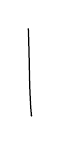
\begin{tikzpicture}[x=1cm,y=1cm]
\draw[line width=0.45pt]
  (0,0.63) .. controls (0.015,0.30) and (0.01,-0.18) .. (0.04,-0.48);
\fill (0.04,-0.48) circle[radius=0.012cm];
\end{tikzpicture}}
\uline{Proposition} $\pi_1(M_{1,1})$ est une extension centrale
de $\pi_1(M_{1,1}')$ par $\{\pm1\}$.

D'autre part, on a les suites exactes,
\deleted{\illegible{5}}
d'homotopie sur $\operatorname{Spec}\mathbb Q$

\scanpage{558}

\diagram{(44)\quad
\begin{tikzcd}[ampersand replacement=\&, column sep=small]
1 \arrow[r,no head] \&
\pi_1(\overline{M}_{1,1})\inserted{{}=\widehat{\mathcal T}_{1,1}^{+}} \arrow[r] \arrow[d] \&
\pi_1(M_{1,1})\inserted{{}=\mathcal E_{1,1}=N_{1,1}} \arrow[r] \arrow[d] \&
\mathbb{\Gamma}_{\mathbb Q} \arrow[r,no head] \arrow[d] \& 1 \\
1 \arrow[r,no head] \& \pi_1(\overline{M'_{1,1}}) \arrow[r,no head] \&
\pi_1(M'_{1,1}) \arrow[r,no head] \& \mathbb{\Gamma}_{\mathbb Q} \arrow[r,no head] \& 1
\end{tikzcd}}

et la théorie transcendante fournit des
isomorphismes \inserted{ext.} canoniques

\diagram{(45)\quad
$\left\{
\begin{tikzcd}[ampersand replacement=\&, column sep=large,row sep=large]
\pi_1(\overline{M}_{1,1}) \arrow[d] \arrow[r,phantom,"\simeq" description]
 \& \mathrm{Sl}(2,\mathbb Z)^{\wedge} \arrow[d] \\
\pi_1(\overline{M'_{1,1}}) \arrow[r,phantom,"\simeq" description]
 \& \mathrm{Sl}(2,\mathbb Z)'^{\wedge}=\mathrm{Sl}(2,\mathbb Z)^{\wedge}/\mathord{\pm}1,
\end{tikzcd}\right.$}

\margin{Attention ne pas confondre $\mathrm{Sl}(2,\mathbb Z)^{\wedge}$ avec $\mathrm{Sl}(2,\widehat{\mathbb Z})$ !!!}

\deleted{\unsure{d'où} \illegible{1} fait que la suite}

On a \unsure{la} compatibilité essentielle
suivante entre (43) (44) (45) : la \unsure{commutativité|compatibilité} de

\diagram{(46)\quad
\begin{tikzcd}[ampersand replacement=\&,column sep=1.8em,row sep=1.25em]
1\arrow[r]
\& \pi_1(\overline M_{1,1})\arrow[r]
   \arrow[d,phantom,"\simeq"{description,rotate=90}]
\& \pi_1(M_{1,1})\arrow[r]\arrow[dd]
   \arrow[r,phantom,"{\deleted{\unsure{\longrightarrow\Gamma_n=\mathrm{Gl}(2,\mathbb Z_n)}}}"{description,yshift=-3.8ex,fill=none,inner sep=0pt}]
\& \mathbb{\Gamma}_{\mathbb Q}\arrow[r]
   \arrow[dd,"{\substack{\chi_n\ \text{caractère}\\\text{cyclotomique}}}"{right}]
\& 1\\
\& \mathrm{Sl}(2,\mathbb Z)^{\wedge}\arrow[d,"\text{surj}"{right}]
\& \& \& \\
1\arrow[r]
\& \mathrm{Sl}(2,\mathbb Z/n\mathbb Z)\arrow[r,hook]
\& \Gamma_n=\mathrm{Gl}(2,\mathbb Z/n\mathbb Z)\arrow[r,"\det"]
\& (\mathbb Z/n\mathbb Z)^*\arrow[r]
\& 1
\end{tikzcd}}

Passant à la limite sur $n$, ceci donne
un diagramme commutatif

\diagram{(47)\quad
\begin{tikzcd}[ampersand replacement=\&, column sep=small]
1 \arrow[r,no head] \&
\bigl(\pi_1(\overline{M}_{1,1})\simeq\mathrm{Sl}(2,\mathbb Z)^{\wedge}\bigr) \arrow[r] \arrow[d,"\text{surj}"'] \&
\pi_1(M_{1,1}) \arrow[r] \arrow[d] \&
\mathbb{\Gamma}_{\mathbb Q} \arrow[r,no head] \arrow[d,"\chi"] \& 1 \\
1 \arrow[r,no head] \& \mathrm{Sl}(2,\widehat{\mathbb Z}) \arrow[r,hook] \&
\mathrm{Gl}(2,\widehat{\mathbb Z}) \arrow[r] \&
\widehat{\mathbb Z}^{*} \arrow[r] \& 1
\end{tikzcd}}

-- diagramme sur lequel nous allons revenir.

\scanpage{559}
\mspage{284}

Pour l'instant je vais exploiter le \inserted{deuxième} isomorphisme (42), $n=2$ :
\[
(48)\qquad
\begin{aligned}
\pi_1(M_{1,1}')\inserted{{}\simeq\deleted{\unsure{\mathcal T_{1,1}^{+}}}N_{1,1}'}
&\simeq\pi_1(M_{1,1}[2]',\Gamma_2=\mathfrak S_3)\\
&\simeq\pi_1(U_{0,3},\mathfrak S_3),
\end{aligned}
\]
où le dernier isomorphisme correspond à
l'isom \inserted{$\operatorname{int}(\sigma_1):$} $\mathfrak S_3\simeq\mathfrak S_3$ explicité dans (40).

On trouve donc bien, comme prévu au
\S\ précédent -- et de façon entièrement
conceptuelle, l'isomorphisme \deleted{de suites}
\deleted{exactes} d'extension

\deleted{(\unsure{49})\quad $\pi_1(M_{1,1}')\simeq\unsure{\widehat{\mathcal T}_{1,1}^{+\,\prime}}\simeq$}

\diagram{(49)\quad
\begin{tikzcd}[ampersand replacement=\&, column sep=small]
1 \arrow[r] \&
\pi_1(\overline{M_{1,1}'})\inserted{{}=\unsure{\widehat{\mathcal T}_{1,1}^{+\,\prime}}\simeq\mathrm{Sl}(2,\mathbb Z)^{\wedge}} \arrow[r] \arrow[d,"\sim"'] \&
\pi_1(M_{1,1}')\inserted{{}\simeq N_{1,1}'} \arrow[r] \arrow[d,"\sim"'] \&
\mathbb{\Gamma}_{\mathbb Q} \arrow[r,no head] \arrow[d,equal] \& 1 \\
1 \arrow[r] \& \pi_1(\overline U_{0,3};\mathfrak S_3) \arrow[r] \arrow[d,"\simeq" description,phantom] \&
\pi_1(U_{0,3},\mathfrak S_3) \arrow[r,no head] \arrow[d,"\simeq" description,phantom] \&
\mathbb{\Gamma}_{\mathbb Q} \arrow[r,no head] \& 1 \\
\& \widehat\Pi_{0,3}' \& \mathcal E_{0,3}'
\end{tikzcd}}

D'ailleurs, reprenant ces réflexions dans le
contexte transcendant, on voit que
cet isomorphisme

\diagram{(50)\quad
\begin{tikzcd}[ampersand replacement=\&, column sep=large]
\widehat\Pi_{0,3}' \arrow[r,"\sim"] \arrow[d,equal] \&
\pi_1(\overline{M_{1,1}'}) \arrow[d,"\simeq" description,phantom] \\
\widehat\Pi_{0,3}/\{\ell_1^2,\ell_\infty^3\} \&
\mathrm{Sl}(2,\mathbb Z)'^{\wedge}=\mathrm{Sl}(2,\mathbb Z)^{\wedge}/\mathord{\pm}1
\end{tikzcd}}

est associé à un isom
\diagram{(51)\quad
$\boxed{\begin{array}{ccc}
\Pi_{0,3}'&\xrightarrow{\sim}&\mathrm{Sl}(2,\mathbb Z)'\simeq\mathrm{Sl}(2,\mathbb Z)/\mathord{\pm}1\\
\Vert&&\\
\Pi_{0,3}/\{\ell_1^{\unsure{2}},\ell_\infty^3\}&&
\end{array}}$}

\scanpage{560}

déduit de l'isom de multiplicités analytiques
complexes
\[
(52)\qquad M_{1,1}^{\mathrm{an}\,\prime}\simeq
(U_{0,3}^{\inserted{\mathrm{an}}}\deleted{\unsure{(\mathbb C)}},\mathfrak S_3)
\]

Il faudrait quand même expliciter
l'hom (51) -- qui n'est défini que
modulo autom. intérieurs, a priori,
par des formules explicites -- alors que
sa définition ici sort de façon purement conceptuelle, ``géométrique'' (au sens
de la géométrie algébrique relative, des
courbes rationnelles et elliptiques sur des
espaces analytiques arbitraires). C'est là
un calcul-clef, \inserted{sûrement instructif,} qui ne devrait pas
présenter de \uline{difficulté} particulière\ldots

J'ai un peu laissé tomber \inserted{en chemin} dans tout
ça le schéma modulaire ``grossier'' $\widetilde M_{1,1}$,
après avoir affirmé qu'il est $\simeq\mathbb E_{\mathbb Z}^{1}$, et
qu'il y a deux sections marquées,
dont les \deleted{points} val. en car. $0$ correspondent
\deleted{\unsure{aux}} \inserted{deux} classes d'isom. de courbes elliptiques
\unsure{anharmoniques}. En termes de l'isom.
\scanpage{561}
\mspage{285}

\[
(53)\qquad
\widetilde M_{1,1}\simeq M_{1,1}[2]'/\Gamma'_2
\simeq U_{0,3}/\mathfrak S_3
\]

\unsure{on|or}\qquad
(valable sur $\mathrm{Spec}\,\mathbb Z[1/2]$)

on trouve bien, au dessus de \inserted{$S=$}$\mathrm{Spec}\,\mathbb Z[1/2]$, que
$\widetilde M_{1,1}$ se déduit d'un schéma relatif \inserted{$Y$,} qui est
\deleted{\illegible{1}} loc. \inserted{(ét)} isom. à $\mathbb P^1_S$,
en enlevant une section $s$ (dont l'existence implique déjà que $Y$ est
\unsure{globalmt|globalement} isom. à $\mathbb P^1_S$ - donc
$Y-s(S)$ isom. à $\mathbb E^1_S$.
Dans cette approche on a donc envie de désigner par $\infty$
(non par $0$, comme en théorie des cartes !) cette section,
qui correspond aux ``points à l'infini'' $\unsure{(0,1,\infty)}$ de
$U_{0,3}$, ou encore au ``\unsure{pt} à l'infini'' de
$\widetilde M_{1,1}$.
Il est d'ailleurs facile de vérifier a priori \unsure{que}
(par la compactification de Deligne-Mumford de $M_{1,1}$ et de
$\widetilde M_{1,1}$) que $\widetilde M_{1,1}$ sur $\mathrm{Spec}\,\mathbb Z$
tt entier est de la forme $Y-\mathrm{Im}\,s$, où $Y$ est lisse propre
sur $\mathrm{Spec}\,\mathbb Z$, et $s$ une section - dès lors ce qu'on
connait p.ex. sur la fibre générique, et le fait que $\mathbb Z$ soit
principal, impliquent que $Y\simeq\mathbb P^1_{\mathbb Z}$, et

\scanpage{562}

qu'on a donc $\widetilde M_{1,1}\simeq\mathbb E^1_{\mathbb Z}$.
Pour \deleted{le} choisir cet isom., on utilise les deux sections de
$\mathbb E^1_{\mathbb Z}$, correspondant aux courbes anharmoniques.
Ces deux sections \uline{ne sont pas} \uline{disjointes}, elles se
rencontrent en car. $2$ et car. $3$.
(Pour ce qui se passe en car. $\ne 2$ i.e. sur
$\mathrm{Spec}\,\mathbb Z[1/2]$, on le voit bien par l'isom $53$ -
\deleted{les} car en car. $3$ les deux orbites
\[
(2,-1,1/2)\quad\text{et}\quad(j,\bar j)
\]
coïncident et se collapsent en un seul et
$\overline{\mathrm m}$ point).
Mais prenant l'une de ces sections comme section nulle
(sauf erreur c'est celle qui correspond à la courbe elliptique la plus
riche en symétries, \unsure{savoir|soit} \unsure{de|le} groupe $\mathbb Z/6\mathbb Z$, qu'on prend -
c'est une question de convention, bien sûr - c'est donc aussi l'orbite
$\{j,\bar j\}$, correspondant à un stabilisateur
$\simeq\mathbb Z/3\mathbb Z$) - cela détermine l'isom
$\widetilde M_{1,1}\simeq\mathbb E^1_{\mathbb Z}$ au signe près.
L'autre section devient alors un entier de la forme
$\pm 2^a3^b$ ($a,b\in\mathbb N^*$ - \uline{entiers} bien déterminés dont
\unsure{je|j'ai} ne sais pas la valeur par \unsure{cœur}), et on achève de

\scanpage{563}
\mspage{286}

normaliser en exigeant que le \uline{signe} soit \uline{plus}. Donc

\uline{Théorème} (pour mémoire - c'est bien connu) Il y a un isom unique
\[
(54)\qquad
\widetilde M_{1,1}\simeq\mathbb E^1_{\mathbb Z},
\]
qui \deleted{donne} en car. $0$ donne à la courbe anharmonique de groupe
d'autom $\mathbb Z/6\mathbb Z$
l'\deleted{\illegible{1}}\inserted{invariant} $0$, et à celle de
groupe $\mathbb Z/4\mathbb Z$ un inv. \deleted{\illegible{1}} $>0$
(qui sera nécessairement $2^a3^b$, avec $a,b\in\mathbb N^*$ bien
déterminés, mais par moi oubliés\ldots).
\margin{$b=3$, cf ci-dessous}

En \unsure{termes} de l'isom
\[
\deleted{\unsure{(55)}}\qquad
\widetilde M_{1,1}\simeq U_{0,3}/\mathfrak S_3
\subset \mathbb P^1/\mathfrak S_3
\]
(valable sur $\mathrm{Spec}\,\mathbb Z[1/2]$)
ceci correspond à \deleted{l'isom} un isom entre
$\mathbb P^1/\mathfrak S_3$ et $\mathbb P^1$ qui à l'orbite
$(0,1,\infty)$ associe $\infty$ (non $0$) et à l'orbite $(j,\bar j)$
associe $0$ (non $\infty$), à l'orbite $(2,-1,1/2)$
\unsure{le fameux} $2^a3^b$ (et non $1$). La fonction
\margin{\uline{invariant} \uline{modulaire}}
\[
(55)\qquad j(\lambda)\in\mathbb Q(\lambda)
\]
qui réalise cet isom, i.e \unsure{le|l'} \deleted{\unsure{hom}} morphisme
\[
(56)\qquad
\mathbb P^1_{\mathbb Z}\xrightarrow{j}\mathbb P^1_{\mathbb Z}
\]
correspondant (de degré $6$, avec
\[
j\circ u=j
\qquad(u\in\mathfrak S_3)
\]
)

\scanpage{564}

est donc \unsure{lié|liée} à celle inspirée de la théorie des cartes,
soit $f(\lambda)$, par
\[
(57)\qquad
j(\lambda)=2^a3^b f(\lambda)^{-1}.
\]

D'ailleurs $f(\lambda)$ \inserted{(ou $j(\lambda)$)} se calcule aisément
par connaissance de ses zéros et de ses pôles,
\inserted{avec leurs multiplicités},
\deleted{\illegible{2}} et la ``normalisation'' par la valeur de $f$
(ou de $j$) sur une des sections $2,-1,1/2$ ; on trouve immédiatement :
\[
(58)\qquad
f(z)=\frac{3^3}{2^2}\frac{z^2(z-1)^2}{(z^2-z+1)^3}
\]
donc
\[
(59)\qquad
j(\lambda)=2^{a+2}3^{b-3}\frac{(z^2-z+1)^3}{z^2(z-1)^2}.
\]

Comme $j(\lambda)$ doit garder un sens en car. $3$ et ne pas être
constante, cela montre d'ailleurs \uline{$b=3$}, donc $(59)$ s'écrit aussi
\[
\deleted{\unsure{(60)}}\qquad
j(\lambda)=2^{a+2}\frac{(z^2-z+1)^3}{z^2(z-1)^2}
\]
- mais on se \unsure{rappellera|rappelle} que cette formule n'est pertinente -
\unsure{ne permet} de calculer
\deleted{un \unsure{discriminant} de}\inserted{l'invariant d'une}
courbe elliptique - qu'en car $\ne 2$, heureusement !
Pour \deleted{\illegible{1}}

\scanpage{565}
\mspage{287}

\deleted{définir}\inserted{décrire}
\[
(60)\qquad
M_{1,1}\longrightarrow\mathbb E^1_{\mathbb Z}
\]
\margin{et en particulier pour déterminer
l'autre invariant modulaire critique
$2^a3^3$, i.e. \uline{déterminer $a$}}
aussi au voisinage de $2$ - disons en car. $\ne 3$ - il faut une étude
des courbes elliptiques qui ne passe plus par la représentation
(de \uline{Legendre}, sauf erreur)
$y^{2}=\sqrt{x(x-1)(x-\lambda)}$, ou encore, par la rigidification de
Jacobi d'échelon $2$, mais par contre par celle d'échelon $3$.

\uline{Remarques} On voit tout de suite que le quotient
$\mathbb P^1_{\mathbb Z}/\mathfrak S_3$ s'identifie à
$\mathbb P^1_{\mathbb Z}$, de façon unique en prenant comme images des
orbites $(0,1,\infty)$ et $(j,\bar j)$ les sections $0$ et $\infty$
(p.ex., en suivant la convention qui correspond à la théorie des cartes),
et en prenant comme image de l'orbite $(2,-1,1/2)$ un
\deleted{entier}\inserted{rationnel} qui soit $>0$.
Ceci est possible a priori, car on note que les \deleted{sections}
orbites $(0,1,\infty)$ et $(j,\bar j)$
\deleted{d'une part, $(0,1,\infty)$ et $(2,-1,1/2)$ d'autre part,}
ne coïncident en aucune caractéristique, donc correspondent à des sections
disjointes de $Y=\mathbb P^1_{\mathbb Z}/\mathfrak S_3$,
tandis que l'orbite \unsure{restante|constante}

\scanpage{566}

$(2,-1,1/2)$ coïncide avec la première en car. $2$, avec la deuxième en
car. $3$ (et ce sont là les seules coïncidences qui peuvent arriver).
On voit donc a priori que la troisième section sera de la forme
$2^\alpha/3^\beta$, avec $\alpha,\beta\in\mathbb N^*$.
Le calcul explicite est d'ailleurs évident, l'hom composé
\[
(61)\qquad
\mathbb P^1_{\mathbb Z}
\xrightarrow{f_1^{\unsure{*|\circ}}}
\mathbb P^1_{\mathbb Z}/\mathfrak S_3
\simeq\mathbb P^1_{\mathbb Z}
\]
doit être de la forme
$f_1^{\unsure{*|\circ}}=c.f^{\unsure{*|\circ}}$, avec la constante
\inserted{$c\in\mathbb Q$} choisie de telle façon que
$cf^{\unsure{*|\circ}}$ \deleted{ait} se réduise bien en
\unsure{ttes} car. (ce qui détermine $c$ \unsure{modulo|mod. le} signe)
et que
\inserted{$f_1(-1)=$}\deleted{\illegible{1}}
$cf^{\unsure{*|\circ}}(-1)$ \inserted{$=c$} $>0$
(ce qui lève l'indétermination du signe).
On trouve alors
\[
(62)\qquad
f_1(\lambda)=
\frac{\lambda^2(\lambda-1)^2}{(\lambda^2-\lambda+1)^{2}}
=\frac{2^2}{3^3}f(\lambda)
\]
donc
\[
(63)\qquad
f_1(-1)=\frac{2^2}{3^3}
\qquad(\text{donc }\alpha=2,\ \beta=3).
\]

Mais on fera attention \deleted{que}
\inserted{qu'au voisinage de la car. $2$,}
ces calculs ne se rapportent plus à $\widetilde M_{1,1}$ et
$\unsure{\widetilde{\widetilde M}|\widetilde{\widehat M}}_{1,1}$,
où la configuration des trois sections
\deleted{\illegible{1}
$\unsure{\Delta_\infty,\Delta_0|\Lambda_\infty,\Lambda_0}$,}
n'est pas la $\overline{\mathrm m}$ \unsure{qu'ici}\ldots

\scanpage{567}
\mspage{288}

Sur la \unsure{lancée} de ces réflexions, il serait naturel de regarder
de plus près le schéma
\[
(64)\qquad
M_{1,1}[4],\quad
\text{sur lequel agit }\Gamma_4=\mathrm{Gl}(2,\mathbb Z/4)
\]
\[
\text{via}\quad \Gamma'_4=\Gamma_4/\pm1
\]
et \unsure{l'homomorphisme} $\otimes$
\[
(65)\qquad
M_{1,1}[4]\longrightarrow M_{1,1}[2]'\simeq U_{0,3}
\]
\inserted{Compatible} \deleted{\illegible{1}}
\[
\Gamma'_4=\mathrm{Gl}(2,\mathbb Z/4)/\pm1
\longrightarrow
\Gamma'_2=\Gamma_2\simeq\mathrm{Gl}(2,\mathbb Z/2)
\simeq\mathfrak S_3
\]
\margin{\diagram{[Au-dessus de la flèche, une inscription biffée :
\deleted{\illegible{1} $\det$}. À gauche de (65), un trait de renvoi
relie le signe $\otimes$ à la note marginale.]}}
\margin{en fait le noyau de l'hom
$\mathrm{Gl}(k,A)$\deleted{\illegible{1}}$\longrightarrow\mathrm{Gl}(k,A/J)$
est tjrs un groupe commutatif $\circledast$
\unsure{si} $J$ est un idéal de carré nul d'un anneau $A$ -
donc ici $\mathrm{Ker}(\mathrm{Gl}(2,\mathbb Z/4\mathbb Z)\longrightarrow
\mathrm{Gl}(2,\mathbb Z/2\mathbb Z))$ est un groupe \uline{commutatif},
et $\overline{\mathrm m}$ un vectoriel sur $\mathbb F_2$ - il est isom. à
$\mathbb F_2^4$}
\margin{$\circledast$ et $\overline{\mathrm m}$ un $A/J$ $(A/J)^4$}

Un calcul immédiat, compte tenu que
\[
(\mathbb Z/4\mathbb Z)^*\simeq\{\pm1\}
\]
, donne
\[
\mathrm{card}\,\Gamma_4
=
2\underbrace{\mathrm{card}\,\mathrm{Sl}(2,\mathbb Z/4\mathbb Z)}
_{8\,\mathrm{card}\,\mathrm{Sl}(2,\mathbb Z/2\mathbb Z)}
=
16.\underbrace{\mathrm{card}\,\Gamma_2}_{6}
\]
donc
\[
(66)\qquad
\mathrm{card}\bigl(\Gamma'_{4,2}
=\mathrm{Ker}(\Gamma'_4\longrightarrow\Gamma'_2)\bigr)=8
\]
i.e. $M_{1,1}[4]$ est un rev. galoisien de $M_{1,1}[2]'$,
de \deleted{groupe} ordre $8$.
Notons qu'il n'est pas géom. connexe sur $\mathbb Q$,
\inserted{\unsure{ou sur $\mathrm{Spec}\,\mathbb Z[1/2]$}},
- puisque $M_{1,1}[4]$ se trouve sur l'extension quadratique
$\mu_4^*$ \deleted{\unsure{$\simeq\mathrm{Spec}$}}, de
$\mathrm{Spec}\,\underbrace{\mathbb Z[1/2]}_{\Lambda}$ disons,
qui n'est autre que $\Lambda[i]$.
\inserted{On a \deleted{\illegible{2}}\inserted{une}}
\deleted{\unsure{Choisissons le point} \illegible{1}}
\inserted{factorisation de
$M_{1,1}[4]\longrightarrow M_{1,1}[2]'$}
\deleted{\unsure{au dessus de}
$\mathrm{Spec}\,\Lambda[i]=\mu_4^*$
sur $\mathrm{Spec}\,\mathbb Z[1/2]$,
nous pouvons distinguer une \unsure{composante connexe}}

\scanpage{568}

\((67)\)
\diagram{
\begin{tikzcd}[ampersand replacement=\&,column sep=large,row sep=large]
M_{1,1}[4]
  \arrow[r,"\text{galoisien}"]
  \arrow[d]
\&
(U_{0,3})_{\unsure{S'}}
  \arrow[r,"\text{galoisien }\unsure{\text{degr. }2}"]
  \arrow[dl]
\&
M_{1,1}[2]'\simeq U_{0,3}
  \arrow[d]
\\
S'=\mu_4^*
  \arrow[rr,"\text{galoisien}","\unsure{\text{degr. }2}"']
\&\&
\mathrm{Spec}\,\mathbb Z[1/2]=S
\end{tikzcd}
}

où maintenant
\[
M_{1,1}[4]\longrightarrow M_{1,1}[2]'_{\unsure{S'}}
=(U_{0,3})_{S'}
\]
est un rev. galoisien de groupe le noyau de
$\Gamma'_{4,2}\xrightarrow{\det}\{\pm1\}$,
\deleted{\illegible{1}}\inserted{ou encore} celui de
$\mathrm{Sl}(2,\mathbb Z/4\mathbb Z)'
\longrightarrow\mathrm{Sl}(2,\mathbb Z/2\mathbb Z)'$,
que nous allons désigner par $S\Gamma'_{4,2}$, qui est d'ordre $4$.

\uline{Proposition} Le groupe
\[
(68)\qquad
S\Gamma_{4,2}
=
\mathrm{Ker}\bigl(
\mathrm{Sl}(2,\mathbb Z/4\mathbb Z)
\longrightarrow
\mathrm{Sl}(2,\mathbb Z/2\mathbb Z)
\bigr)
\]
est isom. à \deleted{\illegible{2}}
$\unsure{\mathfrak{sl}}(2,\mathbb F_2)$
(groupe des matrices à trace nulle à coeff. dans $\mathbb F_2$),
\inserted{avec \unsure{l'op. évidente|les op. évidentes}
de $\mathrm{Sl}(2,\mathbb F_2)$ dessus,}
et le ss-gp $\pm1$ correspond aux matrices scalaires -
le quotient \deleted{\unsure{est}}\inserted{$S\Gamma'_{4,2}$ des deux}
isomorphe à \deleted{\illegible{1}} $\mathbb F_2^2$
(de façon idiote et pas canonique du tout !).
\margin{\uline{NB} C'est les $4$ supplémentaires de ce \unsure{ss-espace}
$\mathbb F_2\unsure{\hookrightarrow|\subset}\unsure{\mathfrak{sl}}(2,\mathbb F_2)$
\deleted{(\unsure{commutatif}}
qui forment un torseur \unsure{sous|sur} le dual de
$V=\unsure{\mathfrak{sl}/\mathbb F_2|\mathfrak{sl}(\mathbb F_2)}$
qui devraient \unsure{correspondre aux quatre} \deleted{\illegible{1}}
relèvements de $\pi_{0,3}\hookrightarrow T^{+\prime}_{1,1}=\mathrm{Sl}(2,\mathbb Z)'$,
\unsure{i.e.|en} $\pi_{0,3}\hookrightarrow\mathrm{Sl}(2,\mathbb Z)$
cf p. $259$, $260$ \unsure{plus haut} sur ces questions}
\deleted{\unsure{enfin}}
Regardant $M_{1,1}[4]$ comme un rev. galoisien de
$M_{1,1}[2]'_{S'}=(U_{0,3})_{S'}$, on trouve
\uline{géométriquement} ``le'' revêtement \uline{abélien} universel de
$U_{0,3}$ de groupe annulé par $2$ (et pour cause), qui a comme groupe
de Galois $(\mathbb F_2)^{\{0,1,\infty\}}/\mathrm{Diagonale}$.

\scanpage{569}
\mspage{289}

Enfin, tout est essentiellement tautologique - mais un calcul amusant à
faire sera de ``\inserted{re}décrire l'action de $\mathrm{Sl}(2,\mathbb F_2)$ sur
$\unsure{\mathfrak{sl}}(2,\mathbb F_2)/\text{matrices scalaires}$''
de façon à l'identifier à l'action de $\mathfrak S_3$ sur
$\mathbb F_2^{\{0,1,\infty\}}/\text{diagonale}$.

Comme revêtement de \deleted{$\unsure{\widetilde M}_{1,1}\simeq M_{1,1}[4]$}
\[
(69)\qquad
\widetilde M_{1,1\,S'}
\simeq M_{1,1}[4]/S\Gamma'_4
\simeq M_{1,1}[2]'_{\unsure{S'}}/\Gamma'_2,
\]
$M_{1,1}[4]$ est un rev. galoisien d'ordre $24$ ($=4.6$),
de groupe $\mathrm{Sl}(2,\mathbb Z/4\mathbb Z)'$.
\deleted{C'est} Ce serait bien \unsure{rare|venu} qu'on n'ait pas un isom
\[
(70)\qquad
\mathrm{Sl}(2,\mathbb Z/4\mathbb Z)'
\simeq\mathfrak S_4
\qquad
(\text{automorphismes de l'octaèdre})
\]
et que $M_{1,1}[4]_{S'}$ en soit le revêtement \deleted{\unsure{étale}}
\deleted{\illegible{1}}
de $\mathbb P^1_{S'}\setminus\{0,1,\infty\}$, avec
ramification compatible avec
$2\{1\}$ \deleted{\illegible{1}} $+3\{\infty\}$,
qui correspond à l'\uline{octaèdre} \unsure{\&} dans la théorie des
cartes - on devrait avoir sur
$S'=\mathrm{Spec}\,\mathbb Z[1/2][i]$
un isom. \inserted{canonique}
\deleted{\unsure{de $\widetilde M_{1,1}$}}
\[
(71)\qquad
M_{1,1}[4]_{S'}\simeq
\text{courbe de Fermat}
\quad
x^2+y^2+z^2=0
\quad(\text{sur }S')
\]
\margin{il vaudrait mieux écrire l'équation de Fermat
ici
$x_0^2+x_1^2+x_\infty^2=0$}
(dont le groupe d'autom. est \unsure{justement} une extension de
$\mathfrak S_3$ par
$\mu_2^{\{0,1,\infty\}}/\mathrm{diag}$ !).

\scanpage{570}

Pour bien faire, il faudrait expliciter la relation entre courbes
elliptiques \inserted{$E/S$} (sur un schéma $S$ au dessus de
$\mathbb Z[1/2][i]$) \unsure{munies} d'une rigidification de Jacobi
d'échelon $4$ $e_1,e_2$ avec $e_1\wedge e_2=[i]^{-1}$, et solutions
``non triviales'' de l'équation
\[
(72)\qquad x^2+y^2+z^2=0
\]
sur $S$ (i.e les systèmes de sections
$x,y,z\in\Gamma(S,\mathcal O_S^*)$ satisfaisant $(72)$, modulo
multiplication par un ``scalaire''
\inserted{$\alpha\in\Gamma(S,\mathcal O_S^*)$}
- ou encore, rompant la symétrie en posant
$X=x/z$, $Y=y/z$, \deleted{\illegible{1}}
les solutions de l'équation
\[
(73)\qquad X^2+Y^2=-1\qquad(=i^2)
\]
$(X,Y\in\Gamma(S,\mathcal O_S^*))$\ldots

On a ainsi interprété $M_{1,1}[2]'$, et
(modulo des vérifications et une étude un peu plus poussée)
$M_{1,1}[4]$, en relation avec \deleted{deux} cartes
\inserted{triangulaires pondérées}
régulières - la carte ``\unsure{dihédrale|dièdrale}''
\inserted{\unsure{d'indice $3$|d'ordre $3$}}
ou carte triangulaire pondérée universelle
(trois sommets $0,1,\infty$,
\figure{[Un contour presque circulaire, avec un ovale horizontal.
Trois points pleins sont marqués sur l'ovale : $0$ à gauche,
$\infty$ sur la branche supérieure à droite, $1$ sur la branche
inférieure à droite. Les trois portions de l'ovale joignent ces
trois points.]}
trois arêtes, deux faces qui sont des triangles, type
$(p,q)=(3,3)$), et la carte \uline{octogonale},
qui est un rev. d'ordre $4$ de celle-ci
\unsure{(}\deleted{\illegible{2}}\inserted{étale}
en dehors des sommets $\{0,1,\infty\}$),

Il y aurait \unsure{lieu} aussi de regarder de
\scanpage{571}
\mspage{290}

plus près les variétés modulaires congruentielles
$M_{1,1}[3]$ et $M_{1,1}[5]$, correspondant à des
groupes modulaires ``géométriques'' :
\[
\unsure{(}\quad
\left\{
\begin{array}{l}
S\Gamma'_3 = \underbrace{\mathrm{Sl}(2,\mathbb F_3)}_{\substack{\text{ordre }4.3.2\\=24}}/\mathord{\pm}1
\quad \text{d'ordre }12\;\underset{\unsure{\deleted{\unsure{\infty}}}}{\phantom{a}}
\subset \underbrace{\mathrm{GP}(1,\mathbb F_3)}_{\text{ordre }24}\simeq\mathfrak S_4
\\[1.5em]
\unsure{\inserted{\text{en fait, on doit avoir } S\Gamma'_4\simeq A_4}}
\\[1.5em]
S\Gamma'_5 = \underbrace{\mathrm{Sl}(2,\mathbb F_5)}_{\substack{\text{ordre }6.5.4\\=120}}/\mathord{\pm}1
\quad \text{d'ordre }60
\subset \underbrace{\mathrm{GP}(1,\mathbb F_5)}_{\text{ordre }120}\simeq\text{groupe du \uline{bi}icosaèdre}
\end{array}
\right.
\tag{74}
\]

Sauf erreur, ces groupes \unsure{sont|\deleted{sont}} \inserted{resp.} les groupes $A_4$ du
\uline{tétraèdre} orienté, et celui $A_5$ de l'icosaèdre
orienté. Si je me rappelle bien, les cas
$n=2,3,4,5$ épuisent les cas de \deleted{\unsure{variétés}}\inserted{courbes} modulaires
congruentielles $M_{1,1}[n]$ qui soient \uline{rationnelles}
-- c'est une chose remarquable que l'on trouve
par eux tous les polyèdres réguliers \inserted{finis} \unsure{à} faces des
triangles \margin{sauf un, à ``arêtes repliées'' -- celui de la figure (76), cf plus bas\ldots} -- il était clair \inserted{\unsure{a priori|a-priori}}, par l'\unsure{isom.|isom} entre
$\mathcal T'_{1,1}$ et le ``groupe cartographique triangula- orienté'' $\pi'_{0,3}$,
qu'on devait retrouver tous
les polyèdres réguliers finis \unsure{à|\deleted{tri}} faces des
triangles de cette façon, mais non pas que
ce soit avec des sous-groupes de \unsure{congruence|congruences},
très exactement. Le tableau obtenu est
alors le suivant

\scanpage{572}

\[
\begin{array}{lll}
\text{groupe }G=S\Gamma'_n & \text{courbe modulaire} & \text{type de polyèdre rég. or.}\\[.5em]
\left\{\begin{array}{l}D_3\simeq\mathfrak S_3\\ A_4\\ \mathfrak S_4\\ A_5\end{array}\right.
&\begin{array}{l}M_{1,1}[2]'\\M_{1,1}[3]\\M_{1,1}[4]\\M_{1,1}[5]\end{array}
&\begin{array}{l}\text{bitriangle sphérique}\\\text{tétraèdre}\\\text{octaèdre}\\\text{icosaèdre}\end{array}
\end{array}
\tag{75}
\]

Comme autres courbes modulaires (pas congruentielles)
rationnelles galoisiennes sur $\widetilde M_{1,1}$, il y aurait encore
les quotients des précédentes par des sous-groupes
invariants des $S\Gamma'_n$, distincts du groupe entier et de $1$.
On trouve comme quotients possibles

\noindent a) Cas $\mathfrak S_3$ ; le quotient $\pm1$ (via signature)

\noindent b) Cas $A_4$ : le quotient $\mathbb Z/3\mathbb Z=C_3$
(via $\mathfrak S_4\to\mathfrak S_3$, induisant $A_4\to C_3$)

\noindent c) Cas $\mathfrak S_4$ : le quotient $\mathfrak S_3$, et le quotient $\{\pm1\}$ de celui-ci.

(Pour d), il n'y a rien, $A_5$ étant un groupe simple)

\deleted{\unsure{Les variétés}}

Les courbes modulaires rationnelles obtenues \unsure{se}
réduisent aux deux cas a) et b) (qui sont
\unsure{retrouvés|retrouvées} dans c)). Dans le cas a), on trouve
le rev. \inserted{quadratique} de $Y=\mathbb P^1(\mathbb C)-\{0,1,\infty\}$, qui est non
ramifié en $\infty$ (car l'indice de ramification doit
diviser $2$ et $3$), qui correspond donc au rev.
\[
\deleted{\unsure{\sqrt{x(x+1)}}}\qquad y=\sqrt{x(x-1)}
\]
et à la carte régulière sphérique de type $(2,1)$
(sommets d'indice $2$, faces d'indice $1$)
\figure{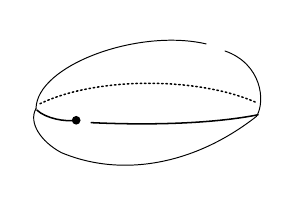
\begin{tikzpicture}[x=1cm,y=1cm,baseline=-0.35ex]
\draw[line width=0.35pt,line cap=round]
(-1.40,0) .. controls (-1.39,0.55) and (-0.10,1.02) .. (0.76,0.82);
\draw[line width=0.35pt,line cap=round]
(1.00,0.73) .. controls (1.46,0.57) and (1.52,0.10) .. (1.40,-0.10)
.. controls (0.61,-0.72) and (-0.32,-0.88) .. (-1.08,-0.56)
.. controls (-1.34,-0.42) and (-1.50,-0.18) .. (-1.40,0);
\draw[densely dotted,line width=0.55pt,line cap=round]
(-1.35,0.06) .. controls (-0.62,0.41) and (0.68,0.40) .. (1.41,0.07);
\draw[line width=0.55pt,line cap=round]
(-1.39,-0.02) .. controls (-1.27,-0.13) and (-1.03,-0.17) .. (-0.90,-0.15);
\fill (-0.89,-0.15) circle[radius=0.055];
\draw[line width=0.55pt,line cap=round]
(-0.70,-0.18) .. controls (0.17,-0.22) and (0.91,-0.18) .. (1.42,-0.08);
\end{tikzpicture}}
\unsure{formé|formée} d'un sommet, \unsure{sur} une arête (équateur) délimitant deux faces qui sont des monogones.

Le cas b) est le rev. cyclique d'ordre $3$ :
ramifié seulement en $0$ et en $\infty$ (en $1$ l'indice de ramification doit être diviseur de $2$ et de $3$,
donc est $1$) donc carte régulière sphérique de

\scanpage{573}
\mspage{291}

type $(3,3)$, avec des arêtes qui sont des boucles
\deleted{\illegible{1}}\inserted{repliées}

(76) \figure{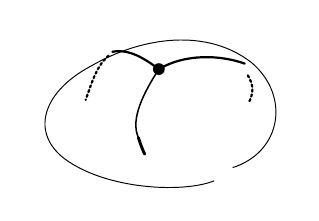
\begin{tikzpicture}[x=1cm,y=1cm,baseline=-0.35ex]
\draw[line width=0.35pt,line cap=round]
(0.89,-0.66) .. controls (1.51,-0.46) and (1.62,0.25) .. (1.13,0.67)
.. controls (0.57,1.11) and (-0.25,1.01) .. (-0.91,0.63)
.. controls (-1.57,0.28) and (-1.71,-0.29) .. (-1.14,-0.62)
.. controls (-0.61,-0.94) and (0.27,-0.98) .. (0.65,-0.83);
\draw[line width=0.8pt,line cap=round]
(-0.05,0.59) .. controls (-0.23,0.72) and (-0.42,0.85) .. (-0.64,0.81);
\draw[densely dotted,line width=0.8pt,line cap=round]
(-0.69,0.76) .. controls (-0.86,0.61) and (-0.91,0.38) .. (-0.98,0.20);
\draw[line width=0.8pt,line cap=round]
(-0.05,0.59) .. controls (0.29,0.79) and (0.73,0.77) .. (1.04,0.66);
\draw[densely dotted,line width=0.8pt,line cap=round]
(1.08,0.51) .. controls (1.16,0.38) and (1.15,0.28) .. (1.09,0.16);
\draw[line width=0.55pt,line cap=round]
(-0.05,0.59) .. controls (-0.23,0.31) and (-0.42,-0.04) .. (-0.31,-0.28);
\draw[line width=1.05pt,line cap=round]
(-0.31,-0.28) .. controls (-0.29,-0.35) and (-0.25,-0.45) .. (-0.23,-0.49);
\fill (-0.05,0.59) circle[radius=0.075];
\end{tikzpicture}}
: $1$ seul sommet,
trois arêtes repliées qui en sortent, une face
triangulaires. [Ces variétés modulaires sont
trop proches de $\widetilde M_{1,1}$ -- avec un groupe
d'autom (quotient de $\Gamma'_\infty=\mathrm{Sl}(2,\unsure{Z|\mathbb Z})$) trop petit,
pour pouvoir être rigidifiantes (il faudrait
que le groupe de Galois-Poincaré du rev.
soit multiple de $12$\inserted{(mult. de $4$ et de $6$ ?!)}, pour que \deleted{\illegible{1}} la courbe modulaire ait une chance d'être rigidifiante. Ces
cas semblent donc nettement moins intéressants.

Il y aurait lieu par ailleurs, dans chacun des
trois cas restants de (75) (mis à part donc le
premier cas, qui correspond à $M_{1,1}[2]'$ et est
à peu près compris), d'expliciter la relation
entre les points des courbes rationnelles
correspondantes, et entre \inserted{courbes elliptiques à} rigidifications de
Jacobi, d'échelon respectivement $3,4,5$. Et il y
a sûrement des choses précises dans Klein,
mais on aimerait faire des choses un peu
plus fines, qui soient valables simultanément
en \unsure{toutes caractéristiques|toute caractéristique} i.e. sur des schémas
de base généraux. Ce souci semble intimement lié à la question des opérations de
$\Gamma_{\mathbb Q}$ sur les classes d'isomorphie des cartes, et

\scanpage{574}

plus particulièrement des cartes sphériques
régulières. C'est assez extraordinaire que
Jean Malgoire, depuis trois ans que la
question est là, n'y ait pas encore touché
-- Dieu sait qu'elle est juteuse !

Complément sur le rapport anharmonique.

Soient $x_1,x_2,x_3,x_4$ des \deleted{variables, \unsure{en|ou} $\infty$}\inserted{sections \inserted{\unsure{partout}} distinctes} de
$\mathbb P^1_S$, on veut construire la section \unsure{correspondante} $\lambda$
de $\unsure{U|\mathbb U}_{0,3}=\mathbb P^1_S-\{0,1,\infty\}_S$.
Soient $a,b,c,d$ sections
(locales) de $\mathcal O_S$, \inserted{avec \deleted{\illegible{1}} $ad-bc$ inversible,} telles que
\[
u=u_{a,b,c,d}:\quad z\longmapsto\frac{az+b}{cz+d}
\tag{77}
\]
transforme $(x_1,x_2,x_3)$ en $(0,1,\infty)$ -- on
aura donc
\[
\lambda=u(x_4).
\tag{78}
\]
Les conditions sur \unsure{$\xi$|\deleted{\illegible{1}}} $(a,b,c,d)$ pour $ux_1=0$ etc sont
\[
\left\{\begin{aligned}
ax_1+b&=0\\
ax_2+b&=cx_2+d\\
cx_3+d&=0
\end{aligned}\right.
\]
qui donnent, si p. ex. $a$ est inversible (sinon, on
peut supposer $\unsure{c}$ inversible\ldots) en résolvant en $b,c,d$
\[
\left\{\begin{aligned}
b&=-ax_1\\
cx_2+d&=a(x_2-x_1)\\
cx_3+d&=0
\end{aligned}\right.
\qquad\left|\begin{aligned}
c&=a\frac{x_2-x_1}{x_2-x_3}\\
d&=-a\frac{x_2-x_1}{x_2-x_3}x_3
\end{aligned}\right.
\]
d'où
\[
\lambda=\frac{ax_4+b}{cx_4+d}
=\frac{a(x_4-x_1)}{a\frac{x_2-x_1}{x_2-x_3}x_4-a\frac{x_2-x_1}{x_2-x_3}x_3}
=\frac{(x_4-x_1)(x_2-x_3)}{(x_2-x_1)(x_4-x_3)}
\]

\scanpage{575}
\mspage{292}

\[
\lambda(x_1,x_2,x_3,x_4)=\frac{(x_4-x_1)(x_2-x_3)}{(x_2-x_1)(x_4-x_3)}
\tag{79}
\]

En tant que fonction rationnelle en $x_1,x_2,x_3,x_4$,
(à coeff. dans un anneau intègre fixé) elle
est caractérisé par les deux propriétés : a) invariance \unsure{p.r.} à une (même) transformation
homographique sur les variables, \inserted{$x_1,x_2,x_3,x_4$,} \deleted{et}
\[
f(ux_1,ux_2,ux_3,ux_4)=f(x_1,x_2,x_3,x_4),
\]
\inserted{et} b)
\[
f(0,1,\infty,x_4)=x_4
\]
(avec un grain de sel pour donner un
sens au premier \unsure{mb.} On a de plus
c) une propriété remarquable de symétrie,
qu'on \deleted{\illegible{1}} explicite en définissant un hom
de $\mathfrak S_4$ dans le groupe homographique
(\unsure{moralement|normalement}, $\mathrm{GP}(1)$)
\deleted{\illegible{1}}
\diagram{
\begin{tikzcd}[ampersand replacement=\&,column sep=large,row sep=large]
\mathfrak S_4 \arrow[rr,"\sigma\mapsto\varphi_\sigma"] \arrow[dr,"\text{épi}","\substack{\text{\unsure{se factorisant}}\\\text{par}}"'] \&\& \mathrm{GP}(1) \\
\& \mathfrak S_3 \arrow[ur] \&
\end{tikzcd}
}
de telle façon qu'on ait
\[
\lambda(x_{\sigma^{-1}1},x_{\sigma^{-1}2},x_{\sigma^{-1}3},x_{\sigma^{-1}4})
=\varphi_\sigma(\lambda(x_1,x_2,x_3,x_4))
\tag{80}
\]
\ldots

\end{document}
